% !BIB program = bibtex

\documentclass[11pt]{article}

% Math libraries
\usepackage[charter,cal=cmcal]{mathdesign} 
\usepackage{amsmath}
% For vertical line in matrix
% https://tex.stackexchange.com/questions/33519/vertical-line-in-matrix-using-latexit
\makeatletter
\renewcommand*\env@matrix[1][*\c@MaxMatrixCols c]{%
    \hskip -\arraycolsep
    \let\@ifnextchar\new@ifnextchar
    \array{#1}}
\makeatother

\usepackage{mathabx}
\usepackage{bm}

% Margins
\usepackage[margin = 1in]{geometry}

% Spacing
\usepackage{setspace}

% Links
\usepackage{hyperref}
\hypersetup{
    colorlinks=true,
    linkcolor=black,
    filecolor=black,      
    urlcolor=blue,
    citecolor=black
}

% Itemize
\renewcommand{\labelitemi}{$\bullet$}
\renewcommand{\labelitemii}{$\circ$}
\renewcommand{\labelitemiii}{$\blackdiamond$} % mathabx package
\renewcommand{\labelitemiv}{$\diamond$}


% Fancy headers
\usepackage{fancyhdr}
\pagestyle{fancy}
\fancyhf{}
\renewcommand{\headrulewidth}{0.3pt}
\headheight 15.0pt
\lhead{Math Workshop Lectures (2019)}
\chead{}
\rhead{Daniel Kent}
%\lfoot{Syllabus version 1.0}
\cfoot{}
\rfoot{\thepage}

% Bibliography
\usepackage[round]{natbib}

% Tikz
\usepackage{tikz}
\usetikzlibrary{arrows}
\usetikzlibrary{decorations.pathreplacing}  
\usetikzlibrary{plotmarks}

% Title
\usepackage{titling}
% Center: https://tex.stackexchange.com/questionkent.249@osu.edus/290432/vertically-center-title-page-article
\renewcommand\maketitlehooka{\null\mbox{}\vfill}
\renewcommand\maketitlehookd{\vfill\null}

\title{Lecture Notes, Math Workshop 2019}
\author{Daniel Kent \\ \texttt{kent.249@osu.edu}}
\date{}

\begin{document}

\maketitle

\newpage

% Table of contents
\tableofcontents
\setcounter{tocdepth}{1} % Show sections
\setcounter{tocdepth}{2} % + subsections
\setcounter{tocdepth}{3} % + subsubsections

\newpage

% Lecture 1: Intro and basic math
\section{Lecture 1: Introduction, Notation, Definitions, and Basic Mathematics}

\subsection{Course Overview}

%What is the purpose of this course? These notes constitute lectures about basic math, linear algebra, and calculus for incoming Ph.D. students to Ohio State's Political Science graduate program. The course runs for two weeks and no mathematical background behind high school algebra is assumed. That said, prior math training among incoming students tends to vary widely. While some students have taken extensive relevant coursework in college, others have not picked up a mathematics textbook since their senior year in high school. The course is designed with this variation in training in mind. Students already exposed to the following concepts will benefit from a review -- there is always more to learn -- and the material covered is intentionally cursory so that those without prior experience are not overwhelmed. Either way, when presented with new mathematical concepts in subsequent statistics or formal theory courses, students will have a set of notes and enough prior exposure to help them figure out what equations represent and how to solve them. 
Although not all of the following material is drawn from \citet{moore2013mathematics}, the overlap is sizeable and intentional. Many thanks to the authors. Some of the examples are also drawn from Jason Morgan's lectures from when I took the same course at the start of graduate school. Many thanks also to Drew Rosenberg.

\onehalfspacing

\subsection{Variables and Constants}

\begin{itemize}
    \item \textbf{Variable}: A concept or a measure that takes different values in a given set.
    \begin{itemize}
        \item E.g., GDP, polity score, party identification, etc.
    \end{itemize}
    \item \textbf{Constant}: A concept or a measure that has a single value for a given set.
\end{itemize}

\subsection{Number Types and Notation}

% https://tex.stackexchange.com/questions/148252/help-drawing-a-very-simple-number-line-using-tikz
\begin{center}
    \begin{tikzpicture}
        \draw[latex-latex] (-5,0) -- (5,0) ; %edit here for the axis
        \foreach \x in  {0} % edit here for the vertical lines
        \draw[shift={(\x,0)},color=black] (0pt,3pt) -- (0pt,-3pt);
        \foreach \x in {0} % edit here for the numbers
        \draw[shift={(\x,0)},color=black] (0pt,0pt) -- (0pt,-3pt) node[below] 
        {$\x$};
        %\draw[*-o] (0.92,0) -- (2.08,0);
        %\draw[very thick] (0.92,0) -- (1.92,0);
    \end{tikzpicture}        
\end{center}

\begin{itemize}
    \itemsep-0.5em 
    \item \textbf{Real numbers}: ($\mathbb{R}$), can be placed anywhere on the line
    \item \textbf{Natural numbers}: ($\mathbb{N}$), positive with no decimal
    \item \textbf{Integer}: ($\mathbb{Z}$), non-decimal, both positive and negative
    \item \textbf{Rational number}: can be expressed as a ratio or fraction
    \item \textbf{Irrational number}: cannot be expressed as a fraction: $\pi$, e
    \item $\bm{\mathbb{R}^k}$ is a k-dimensional space
\end{itemize}

\subsection{Intervals}

\begin{itemize}
    \itemsep-0.5em 
    \item \textbf{Open}: $(-1,2)$, does not include endpoints, so greater than $-1$ and less than $2$. 
    \item \textbf{Closed}: $[-1,2]$, includes endpoints: greater than or equal to $-1$ and less than or equal to $2$.
    \begin{tikzpicture}
        \draw[latex-latex] (-3,0) -- (3,0) ; %edit here for the axis
        \foreach \x in  {0} % edit here for the vertical lines
        \draw[shift={(\x,0)},color=black] (0pt,3pt) -- (0pt,-3pt);
        \foreach \x in {0} % edit here for the numbers
        \draw[shift={(\x,0)},color=black] (0pt,0pt) -- (0pt,-3pt) node[below] 
        {$\x$};
        \draw[thin, yshift=2ex]  (-1,0) -- (2,0);
        \draw[thin] (-1,0.2) -- (-1,0.5);
        \draw[thin] (2,0.2) -- (2,0.5);
    \end{tikzpicture}
    \item \textbf{Half-closed}: $(-1,2]$, includes endpoints: greater than or equal to $-1$ and less than or equal to $2$.
    \begin{tikzpicture}
        \draw[latex-latex] (-3,0) -- (3,0) ; %edit here for the axis
        \foreach \x in  {0} % edit here for the vertical lines
        \draw[shift={(\x,0)},color=black] (0pt,3pt) -- (0pt,-3pt);
        \foreach \x in {0} % edit here for the numbers
        \draw[shift={(\x,0)},color=black] (0pt,0pt) -- (0pt,-3pt) node[below] 
        {$\x$};
        \draw[thin, yshift=2ex]  (-1,0) -- (2,0);
        \draw (-1.05,0.35) circle[radius=2pt, fill = white];
        \draw[thin] (2,0.2) -- (2,0.5);
    \end{tikzpicture}
\end{itemize}

\subsection{Levels of measurement}

\begin{itemize}
    \itemsep-0.5em 
    \item \textbf{Nominal}: No mathematical relationship among the values
    \vspace{-0.75em}
    \begin{itemize}
        \item E.g., race, gender, country, party
    \end{itemize}
    \item \textbf{Ordinal}: Ranking, but cannot do arithmetic because the distance between values is not equal.
    \vspace{-0.75em}
    \begin{itemize}
        \item E.g., K-12, age cohort, ideology (left-to-right)
    \end{itemize}
    \item \textbf{Interval}: Fixed differences, but zero is arbitrary
    \vspace{-0.75em}
    \begin{itemize}
        \item E.g., temperature, date/time
    \end{itemize}
    \item \textbf{Ratio}: Fixed differences with a true zero
    \vspace{-0.75em}
    \begin{itemize}
        \item E.g., age, length, income, votes
    \end{itemize}
\end{itemize}

\subsection{Sets}

\begin{itemize}
    \itemsep-0.5em 
    \item A \textbf{set}, $S = \{\}$, is a collection of elements.
    \begin{itemize}
        \item Order does not matter: $S = \{x,y,z\} = \{z,y,x\}$
        \begin{itemize}
            \item $x \in S$, meaning $x$ is an element of $S$
            \item $a \notin S$, meaning $a$ is not an element of $S$
        \end{itemize}
    \end{itemize}
    \item Other examples:
    \begin{itemize}
        \item $\mathbb{Z} = \{..., -2, -1, 0, 1, 2, ...\}$ or $\{x|x\text{ is an integer}\}$
        \item $T = \{x|8 \geq x \geq 7 \}$ or $T = [7,8]$
    \end{itemize}
    \item Set notation:
    \begin{itemize}
        \item $S = \{x,y,z\}$, $T = \{a,b,x\}$, $N = \{a,b\}$
        \begin{itemize}
            \item Intersection: $T \cap S = \{x\}$
            \begin{itemize}
                \item $N \cap S = \emptyset$: ``empty set''
            \end{itemize}
            \item Union: $N \cup S = \{a,b,x,y,z\}$
            \item Complement (not in the set): $(T \cap S)^c = \{a,b,y,z\}$
        \end{itemize}
        \item $\mathbb{U}$: universal set, all possible values
        \item $A = \{x,y\}$
        \begin{itemize}
            \item $A \subset S$: ``A is a subset of S''
            \item If $\not\subset$, then not a subset of. All subsets of $A$: $\{x\}$, $\{y\}$, $\{\emptyset\}$, $\{x,y\}$
        \end{itemize}
    \end{itemize}
    \item Transitivity:
    \begin{itemize}
        \item If $Z \in Q$ and $Q \in R$, then $Z \in R$
    \end{itemize}
    \item Disjoint:
    \begin{itemize}
        \item No elements in common, more formally, two sets are disjoint if the intercept of sets is the null set: $N \cap S = \{ \emptyset \}$
    \end{itemize}  
\end{itemize}

\subsection{Independent and Dependent Variables}

Let $y = f(x)$, where $y$ is the outcome and $x$ the input.

\begin{itemize}
    \item \textbf{Independent variable}: the input -- $x$
    \item \textbf{Dependent variable}: outcome -- $y$
\end{itemize}

\noindent In a linear model, i.e. $y = \alpha + \beta x$, the dependent variable is $y$ and the independent variable is $x$.

\subsection{Functions}

\begin{itemize}
    \item $f(x) = y$
    \item \textbf{Constant function}: a function whose outcome is the same no matter the input. If $f(x) = c$, then no matter $x$ the output is $c$.
    \item \textbf{Polynomial function}: $y = a + bx + cx^2$ 
    \item \textbf{Rational function}: can be defined by a fraction (ratio):
    \begin{equation*}
        f(x,y) = \frac{a + bx^2}{1 + y}
    \end{equation*} 
\end{itemize}

\subsection{Inequalities and Absolute Values}

\[ |x| = \sqrt{x^2} = \begin{cases} 
    x & \text{if } x > 0 \\
    -x & \text{if } x < 0 \\
    0 & \text{if } x = 0 
\end{cases} \]

\noindent Useful properties:

\begin{itemize}
    \itemsep-0.25em 
    \item $|m| + |n| \geq |m + n|$
    \item $|m| \times |n| = |m \times n|$
\end{itemize}

\subsection{Exponent Rules}

\begin{itemize}
    \itemsep-0.25em 
    \item $x^n = x \cdot x \cdot x \cdot x \cdot ... \cdot x$ $n$ times; $2^2 = 2 \cdot 2 = 4$
    \item $x^0 = 1$
    \item $x^m \cdot x^n = x^{m+n}$
    \item $\frac{x^m}{x^n} = x^{m-n}$
    \item $\frac{1}{x^m} = x^{-m}$
    \item $x^1 = x$
    \item $x^{\frac{1}{m}} = \sqrt[m]{x}$
    \item $(x^m)^n = x^{m \cdot n}$
    \item $x^m \cdot y^m = (xy)^m$
\end{itemize}

\noindent But:

\begin{itemize}
    \item $x^m + y^n \neq (x + y)^{m + n}$
\end{itemize}

\subsection{Commutative, Associative, and Distributive Laws}

\begin{itemize}
    \itemsep-0.5em 
    \item \textbf{Associative property}: rewriting the parentheses does not change the outcome
    \begin{itemize}
        \item $(a + b) + c = a + (b + c)$
        \item $(a \cdot b) \cdot c = a \cdot (b \cdot c)$
    \end{itemize}
    \item \textbf{Commutative property}: order of operands (inputs) does not change the outcome
    \begin{itemize}
        \item $a + b = b + a$
        \item $a \cdot b = b \cdot a$
    \end{itemize}
    \item \textbf{Distributive property}:
    \begin{itemize}
        \item $a(b + c) = ab + ac$
    \end{itemize}
\end{itemize}

\noindent Also relevant:

\begin{itemize}
    \itemsep-0.5em 
    \item \textbf{Inverse property}: 
    \begin{itemize}
        \item For any $x$, there exists a $-x$ such that $-x + x = 0$.
        \begin{itemize}
            \item Formally\footnote{$\exists$ = `there exists'}: $\exists(-x) \text{ s.t. } -x + x = 0$
        \end{itemize}
        \item For any $x$, there exists a $x^{-1}$ such that $x \cdot x^{-1} = 1$.
        \begin{itemize}
            \item Formally: $\exists(x^{-1}) \text{ s.t. } x^{-1} \cdot x = 1$
        \end{itemize}
    \end{itemize}

    \item \textbf{Identity property}:
    \begin{itemize}
        \item $\exists(0) \text{ s.t. } x + 0 = x$
        \item $\exists(1) \text{ s.t. } x \cdot 1 = x$
        \item Commonly, we see: $\text{I}(x) = x$
    \end{itemize}

\end{itemize}

\newpage

% Lecture 2: Basic math 2
\section{Lecture 2: Basic Mathematics II}

\subsection{Summation Operator}

\begin{itemize}
    \item Consider a set $X = \{x_1, x_2, ..., x_n\}$
    \begin{itemize}
        \item $\sum\limits_{i = 1}^{n} x_i = x_1 + x_2 + ... + x_n$
        \begin{itemize}
            \item ``The sum of $x_i$, over the range from $i=l$ through $i = n$.''
        \end{itemize}
    \end{itemize}
    \item Let $Y = \{y_1, y_2, ..., y_n\}$ 
    \begin{itemize}
        \item $\sum\limits_{i=1}^n x_iy_i = x_1y_1 + x_2y_2 + ... + x_ny_n$ 
        \begin{itemize}
            \item Here, we sum the outcome of $x_iy_i$ $n$ times.
        \end{itemize}
    \end{itemize}
    \item But, what if there is more than one summation operator and subscript?
    \vspace{-1em}
    \begin{align*}
        \Sigma_{j=1}^m \Sigma_{i=1}^n x_iy_j 
        & = (y_1x_1 + y_1x_2 + ... + y_1x_n)   \\
        & + (y_2x_1 + y_2x_2 + ... + y_2x_n) \\
        & + ... + (y_mx_1 + y_mx_2 + ... + y_mx_n)
    \end{align*}
    We have $m$ parentheses, with $n$ $x$'s in each parenthesis. We end up summing each combination of $x_i$ and $y_j$.
    \item What if there is a constant, $c$? Drawing upon the \emph{distributive property}:
    \begin{itemize}
        \item $\sum\limits_{i = 1}^{n} cx_i = cx_1 + cx_2 + ... + cx_n = c\sum\limits_{i = 1}^{n} x_i$
    \end{itemize}
    \item The \emph{associative property} can also be applied to summation:
    \begin{itemize}
        \item $\sum\limits_{i=1}^n (x_i + y_i) = (x_1 + y_1) + (x_2 + y_2)
            + ... + (x_n + y_n) = \sum\limits_{i=1}^n x_i + \sum\limits_{i=1}^n y_i$
    \end{itemize}
\end{itemize}

\subsection{Product Operator}

\begin{itemize}
    \item $X = \{x_1, x_2, ..., x_n\}$ and $Y = \{y_1, y_2, ..., y_n\}$ 
    \item $\prod\limits_{i=1}^n x_i = x_1 \cdot x_2 \cdot ... \cdot x_n$
    \item $\prod\limits_{i=1}^n (x_i + y_i) = (x_1 + y_1)(x_2 + y_2) ...
        (x_n + y_n)$
    \begin{itemize}
        \item We can't split $(x_i + y_i)$ like in summation. Instead, we multiply $(x_i + y_i)$ repeatedly.
    \end{itemize}
    \item What about a constant? 
    \begin{itemize}
        \item $\prod\limits_{i = 1}^{n} cx_i = (cx_1)(cx_2) \cdot ... \cdot
            (cx_n) = c^n\prod\limits_{i = 1}^{n} x_i$
    \end{itemize}
    We can move $c$ to the front, but we have to exponentiate it to $c^n$.
\end{itemize}

\subsection{Factorials, Permutations, and Combinations}

Most of our quantitative coursework is about modeling probabilities, where: 

\begin{equation*}
    \text{probability} = \frac{\# \text{occurences}}{\# \text{possibilities}}
\end{equation*}

\noindent For both the numerator and denominator we are dealing with \emph{counting} the number of relevant outcomes. Factorials, permutations, and combinations are foundational concepts when it comes to counting. 

\begin{itemize}
    \item Some useful illustrations/properties:
    \begin{itemize}
        \item $0! = 1$ 
        \item $x! = x \cdot (x-1) \cdot (x-2) \cdot ... \cdot 0!$
        \item $2! = 2 \cdot 1$
        \item $3! = 3 \cdot 2 \cdot 1$
        \item $10! = 10 \cdot 9 \cdot 8 \cdot 7 \cdot 6 \cdot ... \cdot 1$ 
        \item If $n$ objects in boxes of size $x$ where \emph{order matters}, then the number of \emph{permutations} is:
        \begin{equation*}
            \frac{n!}{(n - x)}
        \end{equation*}
        \item If order does not matter, then the number of \emph{combinations} is:
        \begin{equation*}
            \frac{n!}{(n - x)! x!} = n C x = {n \choose x }
        \end{equation*}
        \begin{itemize}
            \item Pronounced: `$n$ choose $x$'
        \end{itemize}
    \end{itemize}
\end{itemize}

\subsection{Solving equations, inequalities, and for roots}

\begin{itemize}
    \item Solving an equation example:
    \begin{align*}
        3x + 4y + 8 & = 0 \\
        4y & = - (3x + 8) \\
        y & = \frac{- (3x + 8)}{4} \\
        y & = -\frac{3}{4}x - 2
    \end{align*}
    
    \noindent We can also write this answer as:
    
    \begin{equation*}
        \{(x,y) \in \mathbb{R} | y = - \frac{3}{4} x - 2 \}
    \end{equation*}
    
    \item Solving an inequality ($x > $, $x \geq y$, $y < x$, $y \leq x$) example:
    \begin{align*}
        -4y & > 2x + 12 \\
        y & < -\frac{2x}{4} - \frac{12}{4} \\
        y & < \frac{x}{2} - 3
    \end{align*}

    \noindent Note that dividing by a negative flips the sign

    \item Solving for a quadratic
    \begin{itemize}
        \item Quadratic formula:
        \begin{align*}
            & ax^2 + bx + c \\
            & x \in \frac{-b \pm \sqrt{b^2 - 4ac}}{2a}
        \end{align*}
        \noindent Example:
        \begin{align*}
            & 1.4x^2 + 3.7x + 1.1 = 0 \\
            & a = 1.4, b = 3.7, c = 1.1 \\
            & x = \frac{-3.7 \pm \sqrt{3.7^2 -
                4 \times 1.4 \times 1.1}}{2.8} \\
            & x = - 0.341 \text{ or } x = -2.301 
        \end{align*}
    \end{itemize}
\end{itemize}

\subsection{Logarithms}

\begin{itemize}
    \item If $y = a^x$, then we can rewrite as $\text{log}_a y = x$
    \item Examples: 
    \begin{itemize}
        \item $\text{log}_e e = 1$, because $e^1 = e$ 
        \item Solving for $x$: 
        \begin{itemize}
            \item If $8 = 2^x$, then $\text{log}_2 8 = x = 3$
        \end{itemize}
    \end{itemize}
    \item \textbf{Rules}
    \begin{itemize}
        \item $\text{log}(m + n) = \text{log}(m) + \text{log}(n)$ 
        \item $\text{log}(\frac{m}{n}) = \text{log}(m) - \text{log}(n)$
        \item $\text{log}(b^a) = a \text{log} b$
        \item $\text{log}b^a = (\text{log}_be)(\text{log}_ea)$ 
        \item $\text{log}b^a = \frac{1}{\text{log}_ab}$
    \end{itemize}
    \item \textbf{Visual}
    
    \resizebox{4in}{!}{
        % Created by tikzDevice version 0.12 on 2019-06-02 23:07:08
% !TEX encoding = UTF-8 Unicode
\begin{tikzpicture}[x=1pt,y=1pt]
\definecolor{fillColor}{RGB}{255,255,255}
\path[use as bounding box,fill=fillColor,fill opacity=0.00] (0,0) rectangle (289.08,289.08);
\begin{scope}
\path[clip] (  0.00,  0.00) rectangle (289.08,289.08);
\definecolor{drawColor}{RGB}{255,255,255}
\definecolor{fillColor}{RGB}{255,255,255}

\path[draw=drawColor,line width= 0.6pt,line join=round,line cap=round,fill=fillColor] (  0.00,  0.00) rectangle (289.08,289.08);
\end{scope}
\begin{scope}
\path[clip] ( 16.80, 20.52) rectangle (283.58,283.58);
\definecolor{fillColor}{RGB}{255,255,255}

\path[fill=fillColor] ( 16.80, 20.52) rectangle (283.58,283.58);
\definecolor{drawColor}{RGB}{0,0,0}

\path[draw=drawColor,line width= 0.6pt,line join=round] (119.88, 32.48) --
	(119.92, 32.81) --
	(119.96, 33.14) --
	(120.00, 33.47) --
	(120.04, 33.79) --
	(120.08, 34.12) --
	(120.12, 34.44) --
	(120.16, 34.77) --
	(120.20, 35.09) --
	(120.24, 35.41) --
	(120.28, 35.73) --
	(120.32, 36.04) --
	(120.36, 36.36) --
	(120.40, 36.68) --
	(120.44, 36.99) --
	(120.48, 37.31) --
	(120.52, 37.62) --
	(120.56, 37.93) --
	(120.60, 38.24) --
	(120.64, 38.55) --
	(120.69, 38.85) --
	(120.73, 39.16) --
	(120.77, 39.47) --
	(120.81, 39.77) --
	(120.85, 40.07) --
	(120.89, 40.37) --
	(120.93, 40.67) --
	(120.97, 40.97) --
	(121.01, 41.27) --
	(121.05, 41.57) --
	(121.09, 41.87) --
	(121.13, 42.16) --
	(121.17, 42.46) --
	(121.21, 42.75) --
	(121.25, 43.04) --
	(121.29, 43.33) --
	(121.33, 43.62) --
	(121.37, 43.91) --
	(121.41, 44.20) --
	(121.45, 44.49) --
	(121.49, 44.77) --
	(121.53, 45.06) --
	(121.57, 45.34) --
	(121.61, 45.63) --
	(121.66, 45.91) --
	(121.70, 46.19) --
	(121.74, 46.47) --
	(121.78, 46.75) --
	(121.82, 47.03) --
	(121.86, 47.31) --
	(121.90, 47.58) --
	(121.94, 47.86) --
	(121.98, 48.13) --
	(122.02, 48.41) --
	(122.06, 48.68) --
	(122.10, 48.95) --
	(122.14, 49.22) --
	(122.18, 49.49) --
	(122.22, 49.76) --
	(122.26, 50.03) --
	(122.30, 50.30) --
	(122.34, 50.57) --
	(122.38, 50.83) --
	(122.42, 51.10) --
	(122.46, 51.36) --
	(122.50, 51.63) --
	(122.54, 51.89) --
	(122.58, 52.15) --
	(122.63, 52.41) --
	(122.67, 52.67) --
	(122.71, 52.93) --
	(122.75, 53.19) --
	(122.79, 53.45) --
	(122.83, 53.70) --
	(122.87, 53.96) --
	(122.91, 54.22) --
	(122.95, 54.47) --
	(122.99, 54.72) --
	(123.03, 54.98) --
	(123.07, 55.23) --
	(123.11, 55.48) --
	(123.15, 55.73) --
	(123.19, 55.98) --
	(123.23, 56.23) --
	(123.27, 56.48) --
	(123.31, 56.73) --
	(123.35, 56.97) --
	(123.39, 57.22) --
	(123.43, 57.47) --
	(123.47, 57.71) --
	(123.51, 57.95) --
	(123.55, 58.20) --
	(123.60, 58.44) --
	(123.64, 58.68) --
	(123.68, 58.92) --
	(123.72, 59.16) --
	(123.76, 59.40) --
	(123.80, 59.64) --
	(123.84, 59.88) --
	(123.88, 60.12) --
	(123.92, 60.36) --
	(123.96, 60.59) --
	(124.00, 60.83) --
	(124.04, 61.06) --
	(124.08, 61.30) --
	(124.12, 61.53) --
	(124.16, 61.76) --
	(124.20, 62.00) --
	(124.24, 62.23) --
	(124.28, 62.46) --
	(124.32, 62.69) --
	(124.36, 62.92) --
	(124.40, 63.15) --
	(124.44, 63.38) --
	(124.48, 63.61) --
	(124.53, 63.83) --
	(124.57, 64.06) --
	(124.61, 64.29) --
	(124.65, 64.51) --
	(124.69, 64.74) --
	(124.73, 64.96) --
	(124.77, 65.18) --
	(124.81, 65.41) --
	(124.85, 65.63) --
	(124.89, 65.85) --
	(124.93, 66.07) --
	(124.97, 66.29) --
	(125.01, 66.51) --
	(125.05, 66.73) --
	(125.09, 66.95) --
	(125.13, 67.17) --
	(125.17, 67.39) --
	(125.21, 67.60) --
	(125.25, 67.82) --
	(125.29, 68.04) --
	(125.33, 68.25) --
	(125.37, 68.47) --
	(125.41, 68.68) --
	(125.45, 68.90) --
	(125.50, 69.11) --
	(125.54, 69.32) --
	(125.58, 69.53) --
	(125.62, 69.75) --
	(125.66, 69.96) --
	(125.70, 70.17) --
	(125.74, 70.38) --
	(125.78, 70.59) --
	(125.82, 70.80) --
	(125.86, 71.00) --
	(125.90, 71.21) --
	(125.94, 71.42) --
	(125.98, 71.63) --
	(126.02, 71.83) --
	(126.06, 72.04) --
	(126.10, 72.24) --
	(126.14, 72.45) --
	(126.18, 72.65) --
	(126.22, 72.86) --
	(126.26, 73.06) --
	(126.30, 73.26) --
	(126.34, 73.47) --
	(126.38, 73.67) --
	(126.42, 73.87) --
	(126.47, 74.07) --
	(126.51, 74.27) --
	(126.55, 74.47) --
	(126.59, 74.67) --
	(126.63, 74.87) --
	(126.67, 75.07) --
	(126.71, 75.26) --
	(126.75, 75.46) --
	(126.79, 75.66) --
	(126.83, 75.86) --
	(126.87, 76.05) --
	(126.91, 76.25) --
	(126.95, 76.44) --
	(126.99, 76.64) --
	(127.03, 76.83) --
	(127.07, 77.03) --
	(127.11, 77.22) --
	(127.15, 77.41) --
	(127.19, 77.60) --
	(127.23, 77.80) --
	(127.27, 77.99) --
	(127.31, 78.18) --
	(127.35, 78.37) --
	(127.39, 78.56) --
	(127.44, 78.75) --
	(127.48, 78.94) --
	(127.52, 79.13) --
	(127.56, 79.32) --
	(127.60, 79.50) --
	(127.64, 79.69) --
	(127.68, 79.88) --
	(127.72, 80.07) --
	(127.76, 80.25) --
	(127.80, 80.44) --
	(127.84, 80.62) --
	(127.88, 80.81) --
	(127.92, 80.99) --
	(127.96, 81.18) --
	(128.00, 81.36) --
	(128.04, 81.55) --
	(128.08, 81.73) --
	(128.12, 81.91) --
	(128.16, 82.09) --
	(128.20, 82.28) --
	(128.24, 82.46) --
	(128.28, 82.64) --
	(128.32, 82.82) --
	(128.36, 83.00) --
	(128.41, 83.18) --
	(128.45, 83.36) --
	(128.49, 83.54) --
	(128.53, 83.72) --
	(128.57, 83.90) --
	(128.61, 84.07) --
	(128.65, 84.25) --
	(128.69, 84.43) --
	(128.73, 84.61) --
	(128.77, 84.78) --
	(128.81, 84.96) --
	(128.85, 85.13) --
	(128.89, 85.31) --
	(128.93, 85.48) --
	(128.97, 85.66) --
	(129.01, 85.83) --
	(129.05, 86.01) --
	(129.09, 86.18) --
	(129.13, 86.35) --
	(129.17, 86.53) --
	(129.21, 86.70) --
	(129.25, 86.87) --
	(129.29, 87.04) --
	(129.34, 87.21) --
	(129.38, 87.38) --
	(129.42, 87.56) --
	(129.46, 87.73) --
	(129.50, 87.90) --
	(129.54, 88.07) --
	(129.58, 88.23) --
	(129.62, 88.40) --
	(129.66, 88.57) --
	(129.70, 88.74) --
	(129.74, 88.91) --
	(129.78, 89.08) --
	(129.82, 89.24) --
	(129.86, 89.41) --
	(129.90, 89.58) --
	(129.94, 89.74) --
	(129.98, 89.91) --
	(130.02, 90.07) --
	(130.06, 90.24) --
	(130.10, 90.40) --
	(130.14, 90.57) --
	(130.18, 90.73) --
	(130.22, 90.90) --
	(130.26, 91.06) --
	(130.31, 91.22) --
	(130.35, 91.39) --
	(130.39, 91.55) --
	(130.43, 91.71) --
	(130.47, 91.87) --
	(130.51, 92.04) --
	(130.55, 92.20) --
	(130.59, 92.36) --
	(130.63, 92.52) --
	(130.67, 92.68) --
	(130.71, 92.84) --
	(130.75, 93.00) --
	(130.79, 93.16) --
	(130.83, 93.32) --
	(130.87, 93.48) --
	(130.91, 93.63) --
	(130.95, 93.79) --
	(130.99, 93.95) --
	(131.03, 94.11) --
	(131.07, 94.27) --
	(131.11, 94.42) --
	(131.15, 94.58) --
	(131.19, 94.74) --
	(131.23, 94.89) --
	(131.28, 95.05) --
	(131.32, 95.20) --
	(131.36, 95.36) --
	(131.40, 95.51) --
	(131.44, 95.67) --
	(131.48, 95.82) --
	(131.52, 95.98) --
	(131.56, 96.13) --
	(131.60, 96.28) --
	(131.64, 96.44) --
	(131.68, 96.59) --
	(131.72, 96.74) --
	(131.76, 96.90) --
	(131.80, 97.05) --
	(131.84, 97.20) --
	(131.88, 97.35) --
	(131.92, 97.50) --
	(131.96, 97.65) --
	(132.00, 97.81) --
	(132.04, 97.96) --
	(132.08, 98.11) --
	(132.12, 98.26) --
	(132.16, 98.41) --
	(132.20, 98.56) --
	(132.25, 98.70) --
	(132.29, 98.85) --
	(132.33, 99.00) --
	(132.37, 99.15) --
	(132.41, 99.30) --
	(132.45, 99.45) --
	(132.49, 99.59) --
	(132.53, 99.74) --
	(132.57, 99.89) --
	(132.61,100.03) --
	(132.65,100.18) --
	(132.69,100.33) --
	(132.73,100.47) --
	(132.77,100.62) --
	(132.81,100.76) --
	(132.85,100.91) --
	(132.89,101.05) --
	(132.93,101.20) --
	(132.97,101.34) --
	(133.01,101.49) --
	(133.05,101.63) --
	(133.09,101.78) --
	(133.13,101.92) --
	(133.18,102.06) --
	(133.22,102.21) --
	(133.26,102.35) --
	(133.30,102.49) --
	(133.34,102.63) --
	(133.38,102.78) --
	(133.42,102.92) --
	(133.46,103.06) --
	(133.50,103.20) --
	(133.54,103.34) --
	(133.58,103.48) --
	(133.62,103.62) --
	(133.66,103.76) --
	(133.70,103.90) --
	(133.74,104.04) --
	(133.78,104.18) --
	(133.82,104.32) --
	(133.86,104.46) --
	(133.90,104.60) --
	(133.94,104.74) --
	(133.98,104.88) --
	(134.02,105.01) --
	(134.06,105.15) --
	(134.10,105.29) --
	(134.15,105.43) --
	(134.19,105.57) --
	(134.23,105.70) --
	(134.27,105.84) --
	(134.31,105.98) --
	(134.35,106.11) --
	(134.39,106.25) --
	(134.43,106.38) --
	(134.47,106.52) --
	(134.51,106.66) --
	(134.55,106.79) --
	(134.59,106.93) --
	(134.63,107.06) --
	(134.67,107.20) --
	(134.71,107.33) --
	(134.75,107.46) --
	(134.79,107.60) --
	(134.83,107.73) --
	(134.87,107.87) --
	(134.91,108.00) --
	(134.95,108.13) --
	(134.99,108.26) --
	(135.03,108.40) --
	(135.07,108.53) --
	(135.12,108.66) --
	(135.16,108.79) --
	(135.20,108.93) --
	(135.24,109.06) --
	(135.28,109.19) --
	(135.32,109.32) --
	(135.36,109.45) --
	(135.40,109.58) --
	(135.44,109.71) --
	(135.48,109.84) --
	(135.52,109.97) --
	(135.56,110.10) --
	(135.60,110.23) --
	(135.64,110.36) --
	(135.68,110.49) --
	(135.72,110.62) --
	(135.76,110.75) --
	(135.80,110.88) --
	(135.84,111.01) --
	(135.88,111.14) --
	(135.92,111.26) --
	(135.96,111.39) --
	(136.00,111.52) --
	(136.04,111.65) --
	(136.09,111.77) --
	(136.13,111.90) --
	(136.17,112.03) --
	(136.21,112.15) --
	(136.25,112.28) --
	(136.29,112.41) --
	(136.33,112.53) --
	(136.37,112.66) --
	(136.41,112.79) --
	(136.45,112.91) --
	(136.49,113.04) --
	(136.53,113.16) --
	(136.57,113.29) --
	(136.61,113.41) --
	(136.65,113.54) --
	(136.69,113.66) --
	(136.73,113.79) --
	(136.77,113.91) --
	(136.81,114.03) --
	(136.85,114.16) --
	(136.89,114.28) --
	(136.93,114.40) --
	(136.97,114.53) --
	(137.01,114.65) --
	(137.06,114.77) --
	(137.10,114.90) --
	(137.14,115.02) --
	(137.18,115.14) --
	(137.22,115.26) --
	(137.26,115.39) --
	(137.30,115.51) --
	(137.34,115.63) --
	(137.38,115.75) --
	(137.42,115.87) --
	(137.46,115.99) --
	(137.50,116.11) --
	(137.54,116.23) --
	(137.58,116.35) --
	(137.62,116.47) --
	(137.66,116.59) --
	(137.70,116.71) --
	(137.74,116.83) --
	(137.78,116.95) --
	(137.82,117.07) --
	(137.86,117.19) --
	(137.90,117.31) --
	(137.94,117.43) --
	(137.99,117.55) --
	(138.03,117.67) --
	(138.07,117.79) --
	(138.11,117.91) --
	(138.15,118.02) --
	(138.19,118.14) --
	(138.23,118.26) --
	(138.27,118.38) --
	(138.31,118.49) --
	(138.35,118.61) --
	(138.39,118.73) --
	(138.43,118.85) --
	(138.47,118.96) --
	(138.51,119.08) --
	(138.55,119.20) --
	(138.59,119.31) --
	(138.63,119.43) --
	(138.67,119.54) --
	(138.71,119.66) --
	(138.75,119.78) --
	(138.79,119.89) --
	(138.83,120.01) --
	(138.87,120.12) --
	(138.91,120.24) --
	(138.96,120.35) --
	(139.00,120.47) --
	(139.04,120.58) --
	(139.08,120.69) --
	(139.12,120.81) --
	(139.16,120.92) --
	(139.20,121.04) --
	(139.24,121.15) --
	(139.28,121.26) --
	(139.32,121.38) --
	(139.36,121.49) --
	(139.40,121.60) --
	(139.44,121.72) --
	(139.48,121.83) --
	(139.52,121.94) --
	(139.56,122.05) --
	(139.60,122.17) --
	(139.64,122.28) --
	(139.68,122.39) --
	(139.72,122.50) --
	(139.76,122.61) --
	(139.80,122.73) --
	(139.84,122.84) --
	(139.88,122.95) --
	(139.93,123.06) --
	(139.97,123.17) --
	(140.01,123.28) --
	(140.05,123.39) --
	(140.09,123.50) --
	(140.13,123.61) --
	(140.17,123.72) --
	(140.21,123.83) --
	(140.25,123.94) --
	(140.29,124.05) --
	(140.33,124.16) --
	(140.37,124.27) --
	(140.41,124.38) --
	(140.45,124.49) --
	(140.49,124.60) --
	(140.53,124.71) --
	(140.57,124.82) --
	(140.61,124.93) --
	(140.65,125.04) --
	(140.69,125.14) --
	(140.73,125.25) --
	(140.77,125.36) --
	(140.81,125.47) --
	(140.85,125.58) --
	(140.90,125.68) --
	(140.94,125.79) --
	(140.98,125.90) --
	(141.02,126.01) --
	(141.06,126.11) --
	(141.10,126.22) --
	(141.14,126.33) --
	(141.18,126.43) --
	(141.22,126.54) --
	(141.26,126.65) --
	(141.30,126.75) --
	(141.34,126.86) --
	(141.38,126.97) --
	(141.42,127.07) --
	(141.46,127.18) --
	(141.50,127.28) --
	(141.54,127.39) --
	(141.58,127.49) --
	(141.62,127.60) --
	(141.66,127.70) --
	(141.70,127.81) --
	(141.74,127.91) --
	(141.78,128.02) --
	(141.83,128.12) --
	(141.87,128.23) --
	(141.91,128.33) --
	(141.95,128.44) --
	(141.99,128.54) --
	(142.03,128.64) --
	(142.07,128.75) --
	(142.11,128.85) --
	(142.15,128.95) --
	(142.19,129.06) --
	(142.23,129.16) --
	(142.27,129.26) --
	(142.31,129.37) --
	(142.35,129.47) --
	(142.39,129.57) --
	(142.43,129.68) --
	(142.47,129.78) --
	(142.51,129.88) --
	(142.55,129.98) --
	(142.59,130.08) --
	(142.63,130.19) --
	(142.67,130.29) --
	(142.71,130.39) --
	(142.75,130.49) --
	(142.80,130.59) --
	(142.84,130.69) --
	(142.88,130.80) --
	(142.92,130.90) --
	(142.96,131.00) --
	(143.00,131.10) --
	(143.04,131.20) --
	(143.08,131.30) --
	(143.12,131.40) --
	(143.16,131.50) --
	(143.20,131.60) --
	(143.24,131.70) --
	(143.28,131.80) --
	(143.32,131.90) --
	(143.36,132.00) --
	(143.40,132.10) --
	(143.44,132.20) --
	(143.48,132.30) --
	(143.52,132.40) --
	(143.56,132.50) --
	(143.60,132.60) --
	(143.64,132.70) --
	(143.68,132.79) --
	(143.72,132.89) --
	(143.77,132.99) --
	(143.81,133.09) --
	(143.85,133.19) --
	(143.89,133.29) --
	(143.93,133.38) --
	(143.97,133.48) --
	(144.01,133.58) --
	(144.05,133.68) --
	(144.09,133.78) --
	(144.13,133.87) --
	(144.17,133.97) --
	(144.21,134.07) --
	(144.25,134.17) --
	(144.29,134.26) --
	(144.33,134.36) --
	(144.37,134.46) --
	(144.41,134.55) --
	(144.45,134.65) --
	(144.49,134.75) --
	(144.53,134.84) --
	(144.57,134.94) --
	(144.61,135.04) --
	(144.65,135.13) --
	(144.69,135.23) --
	(144.74,135.32) --
	(144.78,135.42) --
	(144.82,135.51) --
	(144.86,135.61) --
	(144.90,135.71) --
	(144.94,135.80) --
	(144.98,135.90) --
	(145.02,135.99) --
	(145.06,136.09) --
	(145.10,136.18) --
	(145.14,136.28) --
	(145.18,136.37) --
	(145.22,136.46) --
	(145.26,136.56) --
	(145.30,136.65) --
	(145.34,136.75) --
	(145.38,136.84) --
	(145.42,136.94) --
	(145.46,137.03) --
	(145.50,137.12) --
	(145.54,137.22) --
	(145.58,137.31) --
	(145.62,137.40) --
	(145.66,137.50) --
	(145.71,137.59) --
	(145.75,137.68) --
	(145.79,137.78) --
	(145.83,137.87) --
	(145.87,137.96) --
	(145.91,138.06) --
	(145.95,138.15) --
	(145.99,138.24) --
	(146.03,138.33) --
	(146.07,138.43) --
	(146.11,138.52) --
	(146.15,138.61) --
	(146.19,138.70) --
	(146.23,138.79) --
	(146.27,138.89) --
	(146.31,138.98) --
	(146.35,139.07) --
	(146.39,139.16) --
	(146.43,139.25) --
	(146.47,139.34) --
	(146.51,139.43) --
	(146.55,139.53) --
	(146.59,139.62) --
	(146.64,139.71) --
	(146.68,139.80) --
	(146.72,139.89) --
	(146.76,139.98) --
	(146.80,140.07) --
	(146.84,140.16) --
	(146.88,140.25) --
	(146.92,140.34) --
	(146.96,140.43) --
	(147.00,140.52) --
	(147.04,140.61) --
	(147.08,140.70) --
	(147.12,140.79) --
	(147.16,140.88) --
	(147.20,140.97) --
	(147.24,141.06) --
	(147.28,141.15) --
	(147.32,141.24) --
	(147.36,141.33) --
	(147.40,141.42) --
	(147.44,141.50) --
	(147.48,141.59) --
	(147.52,141.68) --
	(147.56,141.77) --
	(147.61,141.86) --
	(147.65,141.95) --
	(147.69,142.04) --
	(147.73,142.12) --
	(147.77,142.21) --
	(147.81,142.30) --
	(147.85,142.39) --
	(147.89,142.48) --
	(147.93,142.56) --
	(147.97,142.65) --
	(148.01,142.74) --
	(148.05,142.83) --
	(148.09,142.91) --
	(148.13,143.00) --
	(148.17,143.09) --
	(148.21,143.18) --
	(148.25,143.26) --
	(148.29,143.35) --
	(148.33,143.44) --
	(148.37,143.52) --
	(148.41,143.61) --
	(148.45,143.70) --
	(148.49,143.78) --
	(148.53,143.87) --
	(148.58,143.96) --
	(148.62,144.04) --
	(148.66,144.13) --
	(148.70,144.22) --
	(148.74,144.30) --
	(148.78,144.39) --
	(148.82,144.47) --
	(148.86,144.56) --
	(148.90,144.64) --
	(148.94,144.73) --
	(148.98,144.82) --
	(149.02,144.90) --
	(149.06,144.99) --
	(149.10,145.07) --
	(149.14,145.16) --
	(149.18,145.24) --
	(149.22,145.33) --
	(149.26,145.41) --
	(149.30,145.50) --
	(149.34,145.58) --
	(149.38,145.67) --
	(149.42,145.75) --
	(149.46,145.83) --
	(149.50,145.92) --
	(149.55,146.00) --
	(149.59,146.09) --
	(149.63,146.17) --
	(149.67,146.26) --
	(149.71,146.34) --
	(149.75,146.42) --
	(149.79,146.51) --
	(149.83,146.59) --
	(149.87,146.67) --
	(149.91,146.76) --
	(149.95,146.84) --
	(149.99,146.92) --
	(150.03,147.01) --
	(150.07,147.09) --
	(150.11,147.17) --
	(150.15,147.26) --
	(150.19,147.34) --
	(150.23,147.42) --
	(150.27,147.50) --
	(150.31,147.59) --
	(150.35,147.67) --
	(150.39,147.75) --
	(150.43,147.84) --
	(150.48,147.92) --
	(150.52,148.00) --
	(150.56,148.08) --
	(150.60,148.16) --
	(150.64,148.25) --
	(150.68,148.33) --
	(150.72,148.41) --
	(150.76,148.49) --
	(150.80,148.57) --
	(150.84,148.65) --
	(150.88,148.74) --
	(150.92,148.82) --
	(150.96,148.90) --
	(151.00,148.98) --
	(151.04,149.06) --
	(151.08,149.14) --
	(151.12,149.22) --
	(151.16,149.30) --
	(151.20,149.39) --
	(151.24,149.47) --
	(151.28,149.55) --
	(151.32,149.63) --
	(151.36,149.71) --
	(151.40,149.79) --
	(151.45,149.87) --
	(151.49,149.95) --
	(151.53,150.03) --
	(151.57,150.11) --
	(151.61,150.19) --
	(151.65,150.27) --
	(151.69,150.35) --
	(151.73,150.43) --
	(151.77,150.51) --
	(151.81,150.59) --
	(151.85,150.67) --
	(151.89,150.75) --
	(151.93,150.83) --
	(151.97,150.91) --
	(152.01,150.99) --
	(152.05,151.07) --
	(152.09,151.14) --
	(152.13,151.22) --
	(152.17,151.30) --
	(152.21,151.38) --
	(152.25,151.46) --
	(152.29,151.54) --
	(152.33,151.62) --
	(152.37,151.70) --
	(152.42,151.78) --
	(152.46,151.85) --
	(152.50,151.93) --
	(152.54,152.01) --
	(152.58,152.09) --
	(152.62,152.17) --
	(152.66,152.25) --
	(152.70,152.32) --
	(152.74,152.40) --
	(152.78,152.48) --
	(152.82,152.56) --
	(152.86,152.63) --
	(152.90,152.71) --
	(152.94,152.79) --
	(152.98,152.87) --
	(153.02,152.95) --
	(153.06,153.02) --
	(153.10,153.10) --
	(153.14,153.18) --
	(153.18,153.25) --
	(153.22,153.33) --
	(153.26,153.41) --
	(153.30,153.49) --
	(153.34,153.56) --
	(153.39,153.64) --
	(153.43,153.72) --
	(153.47,153.79) --
	(153.51,153.87) --
	(153.55,153.95) --
	(153.59,154.02) --
	(153.63,154.10) --
	(153.67,154.18) --
	(153.71,154.25) --
	(153.75,154.33) --
	(153.79,154.40) --
	(153.83,154.48) --
	(153.87,154.56) --
	(153.91,154.63) --
	(153.95,154.71) --
	(153.99,154.78) --
	(154.03,154.86) --
	(154.07,154.93) --
	(154.11,155.01) --
	(154.15,155.09) --
	(154.19,155.16) --
	(154.23,155.24) --
	(154.27,155.31) --
	(154.31,155.39) --
	(154.36,155.46) --
	(154.40,155.54) --
	(154.44,155.61) --
	(154.48,155.69) --
	(154.52,155.76) --
	(154.56,155.84) --
	(154.60,155.91) --
	(154.64,155.99) --
	(154.68,156.06) --
	(154.72,156.14) --
	(154.76,156.21) --
	(154.80,156.28) --
	(154.84,156.36) --
	(154.88,156.43) --
	(154.92,156.51) --
	(154.96,156.58) --
	(155.00,156.66) --
	(155.04,156.73) --
	(155.08,156.80) --
	(155.12,156.88) --
	(155.16,156.95) --
	(155.20,157.02) --
	(155.24,157.10) --
	(155.29,157.17) --
	(155.33,157.25) --
	(155.37,157.32) --
	(155.41,157.39) --
	(155.45,157.47) --
	(155.49,157.54) --
	(155.53,157.61) --
	(155.57,157.69) --
	(155.61,157.76) --
	(155.65,157.83) --
	(155.69,157.90) --
	(155.73,157.98) --
	(155.77,158.05) --
	(155.81,158.12) --
	(155.85,158.20) --
	(155.89,158.27) --
	(155.93,158.34) --
	(155.97,158.41) --
	(156.01,158.49) --
	(156.05,158.56) --
	(156.09,158.63) --
	(156.13,158.70) --
	(156.17,158.78) --
	(156.21,158.85) --
	(156.26,158.92) --
	(156.30,158.99) --
	(156.34,159.06) --
	(156.38,159.14) --
	(156.42,159.21) --
	(156.46,159.28) --
	(156.50,159.35) --
	(156.54,159.42) --
	(156.58,159.49) --
	(156.62,159.57) --
	(156.66,159.64) --
	(156.70,159.71) --
	(156.74,159.78) --
	(156.78,159.85) --
	(156.82,159.92) --
	(156.86,159.99) --
	(156.90,160.06) --
	(156.94,160.14) --
	(156.98,160.21) --
	(157.02,160.28) --
	(157.06,160.35) --
	(157.10,160.42) --
	(157.14,160.49) --
	(157.18,160.56) --
	(157.23,160.63) --
	(157.27,160.70) --
	(157.31,160.77) --
	(157.35,160.84) --
	(157.39,160.91) --
	(157.43,160.98) --
	(157.47,161.05) --
	(157.51,161.12) --
	(157.55,161.19) --
	(157.59,161.26) --
	(157.63,161.33) --
	(157.67,161.40) --
	(157.71,161.47) --
	(157.75,161.54) --
	(157.79,161.61) --
	(157.83,161.68) --
	(157.87,161.75) --
	(157.91,161.82) --
	(157.95,161.89) --
	(157.99,161.96) --
	(158.03,162.03) --
	(158.07,162.10) --
	(158.11,162.17) --
	(158.15,162.24) --
	(158.20,162.31) --
	(158.24,162.38) --
	(158.28,162.45) --
	(158.32,162.51) --
	(158.36,162.58) --
	(158.40,162.65) --
	(158.44,162.72) --
	(158.48,162.79) --
	(158.52,162.86) --
	(158.56,162.93) --
	(158.60,163.00) --
	(158.64,163.06) --
	(158.68,163.13) --
	(158.72,163.20) --
	(158.76,163.27) --
	(158.80,163.34) --
	(158.84,163.41) --
	(158.88,163.48) --
	(158.92,163.54) --
	(158.96,163.61) --
	(159.00,163.68) --
	(159.04,163.75) --
	(159.08,163.82) --
	(159.13,163.88) --
	(159.17,163.95) --
	(159.21,164.02) --
	(159.25,164.09) --
	(159.29,164.15) --
	(159.33,164.22) --
	(159.37,164.29) --
	(159.41,164.36) --
	(159.45,164.42) --
	(159.49,164.49) --
	(159.53,164.56) --
	(159.57,164.63) --
	(159.61,164.69) --
	(159.65,164.76) --
	(159.69,164.83) --
	(159.73,164.89) --
	(159.77,164.96) --
	(159.81,165.03) --
	(159.85,165.10) --
	(159.89,165.16) --
	(159.93,165.23) --
	(159.97,165.30) --
	(160.01,165.36) --
	(160.05,165.43) --
	(160.10,165.50) --
	(160.14,165.56) --
	(160.18,165.63) --
	(160.22,165.70) --
	(160.26,165.76) --
	(160.30,165.83) --
	(160.34,165.89) --
	(160.38,165.96) --
	(160.42,166.03) --
	(160.46,166.09) --
	(160.50,166.16) --
	(160.54,166.22) --
	(160.58,166.29) --
	(160.62,166.36) --
	(160.66,166.42) --
	(160.70,166.49) --
	(160.74,166.55) --
	(160.78,166.62) --
	(160.82,166.69) --
	(160.86,166.75) --
	(160.90,166.82) --
	(160.94,166.88) --
	(160.98,166.95) --
	(161.02,167.01) --
	(161.07,167.08) --
	(161.11,167.14) --
	(161.15,167.21) --
	(161.19,167.27) --
	(161.23,167.34) --
	(161.27,167.40) --
	(161.31,167.47) --
	(161.35,167.53) --
	(161.39,167.60) --
	(161.43,167.66) --
	(161.47,167.73) --
	(161.51,167.79) --
	(161.55,167.86) --
	(161.59,167.92) --
	(161.63,167.99) --
	(161.67,168.05) --
	(161.71,168.12) --
	(161.75,168.18) --
	(161.79,168.25) --
	(161.83,168.31) --
	(161.87,168.37) --
	(161.91,168.44) --
	(161.95,168.50) --
	(161.99,168.57) --
	(162.04,168.63) --
	(162.08,168.69) --
	(162.12,168.76) --
	(162.16,168.82) --
	(162.20,168.89) --
	(162.24,168.95) --
	(162.28,169.01) --
	(162.32,169.08) --
	(162.36,169.14) --
	(162.40,169.21) --
	(162.44,169.27) --
	(162.48,169.33) --
	(162.52,169.40) --
	(162.56,169.46) --
	(162.60,169.52) --
	(162.64,169.59) --
	(162.68,169.65) --
	(162.72,169.71) --
	(162.76,169.78) --
	(162.80,169.84) --
	(162.84,169.90) --
	(162.88,169.97) --
	(162.92,170.03) --
	(162.96,170.09) --
	(163.01,170.15) --
	(163.05,170.22) --
	(163.09,170.28) --
	(163.13,170.34) --
	(163.17,170.41) --
	(163.21,170.47) --
	(163.25,170.53) --
	(163.29,170.59) --
	(163.33,170.66) --
	(163.37,170.72) --
	(163.41,170.78) --
	(163.45,170.84) --
	(163.49,170.91) --
	(163.53,170.97) --
	(163.57,171.03) --
	(163.61,171.09) --
	(163.65,171.15) --
	(163.69,171.22) --
	(163.73,171.28) --
	(163.77,171.34) --
	(163.81,171.40) --
	(163.85,171.46) --
	(163.89,171.53) --
	(163.94,171.59) --
	(163.98,171.65) --
	(164.02,171.71) --
	(164.06,171.77) --
	(164.10,171.84) --
	(164.14,171.90) --
	(164.18,171.96) --
	(164.22,172.02) --
	(164.26,172.08) --
	(164.30,172.14) --
	(164.34,172.20) --
	(164.38,172.27) --
	(164.42,172.33) --
	(164.46,172.39) --
	(164.50,172.45) --
	(164.54,172.51) --
	(164.58,172.57) --
	(164.62,172.63) --
	(164.66,172.69) --
	(164.70,172.76) --
	(164.74,172.82) --
	(164.78,172.88) --
	(164.82,172.94) --
	(164.86,173.00) --
	(164.91,173.06) --
	(164.95,173.12) --
	(164.99,173.18) --
	(165.03,173.24) --
	(165.07,173.30) --
	(165.11,173.36) --
	(165.15,173.42) --
	(165.19,173.48) --
	(165.23,173.54) --
	(165.27,173.60) --
	(165.31,173.66) --
	(165.35,173.73) --
	(165.39,173.79) --
	(165.43,173.85) --
	(165.47,173.91) --
	(165.51,173.97) --
	(165.55,174.03) --
	(165.59,174.09) --
	(165.63,174.15) --
	(165.67,174.21) --
	(165.71,174.27) --
	(165.75,174.33) --
	(165.79,174.39) --
	(165.83,174.45) --
	(165.88,174.50) --
	(165.92,174.56) --
	(165.96,174.62) --
	(166.00,174.68) --
	(166.04,174.74) --
	(166.08,174.80) --
	(166.12,174.86) --
	(166.16,174.92) --
	(166.20,174.98) --
	(166.24,175.04) --
	(166.28,175.10) --
	(166.32,175.16) --
	(166.36,175.22) --
	(166.40,175.28) --
	(166.44,175.34) --
	(166.48,175.40) --
	(166.52,175.45) --
	(166.56,175.51) --
	(166.60,175.57) --
	(166.64,175.63) --
	(166.68,175.69) --
	(166.72,175.75) --
	(166.76,175.81) --
	(166.80,175.87) --
	(166.85,175.93) --
	(166.89,175.98) --
	(166.93,176.04) --
	(166.97,176.10) --
	(167.01,176.16) --
	(167.05,176.22) --
	(167.09,176.28) --
	(167.13,176.33) --
	(167.17,176.39) --
	(167.21,176.45) --
	(167.25,176.51) --
	(167.29,176.57) --
	(167.33,176.63) --
	(167.37,176.68) --
	(167.41,176.74) --
	(167.45,176.80) --
	(167.49,176.86) --
	(167.53,176.92) --
	(167.57,176.97) --
	(167.61,177.03) --
	(167.65,177.09) --
	(167.69,177.15) --
	(167.73,177.21) --
	(167.78,177.26) --
	(167.82,177.32) --
	(167.86,177.38) --
	(167.90,177.44) --
	(167.94,177.49) --
	(167.98,177.55) --
	(168.02,177.61) --
	(168.06,177.67) --
	(168.10,177.72) --
	(168.14,177.78) --
	(168.18,177.84) --
	(168.22,177.90) --
	(168.26,177.95) --
	(168.30,178.01) --
	(168.34,178.07) --
	(168.38,178.13) --
	(168.42,178.18) --
	(168.46,178.24) --
	(168.50,178.30) --
	(168.54,178.35) --
	(168.58,178.41) --
	(168.62,178.47) --
	(168.66,178.52) --
	(168.70,178.58) --
	(168.75,178.64) --
	(168.79,178.69) --
	(168.83,178.75) --
	(168.87,178.81) --
	(168.91,178.87) --
	(168.95,178.92) --
	(168.99,178.98) --
	(169.03,179.03) --
	(169.07,179.09) --
	(169.11,179.15) --
	(169.15,179.20) --
	(169.19,179.26) --
	(169.23,179.32) --
	(169.27,179.37) --
	(169.31,179.43) --
	(169.35,179.49) --
	(169.39,179.54) --
	(169.43,179.60) --
	(169.47,179.65) --
	(169.51,179.71) --
	(169.55,179.77) --
	(169.59,179.82) --
	(169.63,179.88) --
	(169.67,179.93) --
	(169.72,179.99) --
	(169.76,180.05) --
	(169.80,180.10) --
	(169.84,180.16) --
	(169.88,180.21) --
	(169.92,180.27) --
	(169.96,180.32) --
	(170.00,180.38) --
	(170.04,180.44) --
	(170.08,180.49) --
	(170.12,180.55) --
	(170.16,180.60) --
	(170.20,180.66) --
	(170.24,180.71) --
	(170.28,180.77) --
	(170.32,180.82) --
	(170.36,180.88) --
	(170.40,180.93) --
	(170.44,180.99) --
	(170.48,181.04) --
	(170.52,181.10) --
	(170.56,181.16) --
	(170.60,181.21) --
	(170.64,181.27) --
	(170.69,181.32) --
	(170.73,181.38) --
	(170.77,181.43) --
	(170.81,181.48) --
	(170.85,181.54) --
	(170.89,181.59) --
	(170.93,181.65) --
	(170.97,181.70) --
	(171.01,181.76) --
	(171.05,181.81) --
	(171.09,181.87) --
	(171.13,181.92) --
	(171.17,181.98) --
	(171.21,182.03) --
	(171.25,182.09) --
	(171.29,182.14) --
	(171.33,182.20) --
	(171.37,182.25) --
	(171.41,182.30) --
	(171.45,182.36) --
	(171.49,182.41) --
	(171.53,182.47) --
	(171.57,182.52) --
	(171.61,182.58) --
	(171.66,182.63) --
	(171.70,182.68) --
	(171.74,182.74) --
	(171.78,182.79) --
	(171.82,182.85) --
	(171.86,182.90) --
	(171.90,182.95) --
	(171.94,183.01) --
	(171.98,183.06) --
	(172.02,183.11) --
	(172.06,183.17) --
	(172.10,183.22) --
	(172.14,183.28) --
	(172.18,183.33) --
	(172.22,183.38) --
	(172.26,183.44) --
	(172.30,183.49) --
	(172.34,183.54) --
	(172.38,183.60) --
	(172.42,183.65) --
	(172.46,183.70) --
	(172.50,183.76) --
	(172.54,183.81) --
	(172.59,183.86) --
	(172.63,183.92) --
	(172.67,183.97) --
	(172.71,184.02) --
	(172.75,184.08) --
	(172.79,184.13) --
	(172.83,184.18) --
	(172.87,184.24) --
	(172.91,184.29) --
	(172.95,184.34) --
	(172.99,184.40) --
	(173.03,184.45) --
	(173.07,184.50) --
	(173.11,184.56) --
	(173.15,184.61) --
	(173.19,184.66) --
	(173.23,184.71) --
	(173.27,184.77) --
	(173.31,184.82) --
	(173.35,184.87) --
	(173.39,184.92) --
	(173.43,184.98) --
	(173.47,185.03) --
	(173.51,185.08) --
	(173.56,185.13) --
	(173.60,185.19) --
	(173.64,185.24) --
	(173.68,185.29) --
	(173.72,185.34) --
	(173.76,185.40) --
	(173.80,185.45) --
	(173.84,185.50) --
	(173.88,185.55) --
	(173.92,185.61) --
	(173.96,185.66) --
	(174.00,185.71) --
	(174.04,185.76) --
	(174.08,185.81) --
	(174.12,185.87) --
	(174.16,185.92) --
	(174.20,185.97) --
	(174.24,186.02) --
	(174.28,186.07) --
	(174.32,186.13) --
	(174.36,186.18) --
	(174.40,186.23) --
	(174.44,186.28) --
	(174.48,186.33) --
	(174.53,186.39) --
	(174.57,186.44) --
	(174.61,186.49) --
	(174.65,186.54) --
	(174.69,186.59) --
	(174.73,186.64) --
	(174.77,186.70) --
	(174.81,186.75) --
	(174.85,186.80) --
	(174.89,186.85) --
	(174.93,186.90) --
	(174.97,186.95) --
	(175.01,187.00) --
	(175.05,187.05) --
	(175.09,187.11) --
	(175.13,187.16) --
	(175.17,187.21) --
	(175.21,187.26) --
	(175.25,187.31) --
	(175.29,187.36) --
	(175.33,187.41) --
	(175.37,187.46) --
	(175.41,187.52) --
	(175.45,187.57) --
	(175.50,187.62) --
	(175.54,187.67) --
	(175.58,187.72) --
	(175.62,187.77) --
	(175.66,187.82) --
	(175.70,187.87) --
	(175.74,187.92) --
	(175.78,187.97) --
	(175.82,188.02) --
	(175.86,188.07) --
	(175.90,188.13) --
	(175.94,188.18) --
	(175.98,188.23) --
	(176.02,188.28) --
	(176.06,188.33) --
	(176.10,188.38) --
	(176.14,188.43) --
	(176.18,188.48) --
	(176.22,188.53) --
	(176.26,188.58) --
	(176.30,188.63) --
	(176.34,188.68) --
	(176.38,188.73) --
	(176.43,188.78) --
	(176.47,188.83) --
	(176.51,188.88) --
	(176.55,188.93) --
	(176.59,188.98) --
	(176.63,189.03) --
	(176.67,189.08) --
	(176.71,189.13) --
	(176.75,189.18) --
	(176.79,189.23) --
	(176.83,189.28) --
	(176.87,189.33) --
	(176.91,189.38) --
	(176.95,189.43) --
	(176.99,189.48) --
	(177.03,189.53) --
	(177.07,189.58) --
	(177.11,189.63) --
	(177.15,189.68) --
	(177.19,189.73) --
	(177.23,189.78) --
	(177.27,189.83) --
	(177.31,189.88) --
	(177.35,189.93) --
	(177.40,189.98) --
	(177.44,190.03) --
	(177.48,190.08) --
	(177.52,190.13) --
	(177.56,190.18) --
	(177.60,190.23) --
	(177.64,190.28) --
	(177.68,190.32) --
	(177.72,190.37) --
	(177.76,190.42) --
	(177.80,190.47) --
	(177.84,190.52) --
	(177.88,190.57) --
	(177.92,190.62) --
	(177.96,190.67) --
	(178.00,190.72) --
	(178.04,190.77) --
	(178.08,190.82) --
	(178.12,190.87) --
	(178.16,190.91) --
	(178.20,190.96) --
	(178.24,191.01) --
	(178.28,191.06) --
	(178.32,191.11) --
	(178.37,191.16) --
	(178.41,191.21) --
	(178.45,191.26) --
	(178.49,191.30) --
	(178.53,191.35) --
	(178.57,191.40) --
	(178.61,191.45) --
	(178.65,191.50) --
	(178.69,191.55) --
	(178.73,191.60) --
	(178.77,191.65) --
	(178.81,191.69) --
	(178.85,191.74) --
	(178.89,191.79) --
	(178.93,191.84) --
	(178.97,191.89) --
	(179.01,191.94) --
	(179.05,191.98) --
	(179.09,192.03) --
	(179.13,192.08) --
	(179.17,192.13) --
	(179.21,192.18) --
	(179.25,192.23) --
	(179.29,192.27) --
	(179.34,192.32) --
	(179.38,192.37) --
	(179.42,192.42) --
	(179.46,192.47) --
	(179.50,192.51) --
	(179.54,192.56) --
	(179.58,192.61) --
	(179.62,192.66) --
	(179.66,192.71) --
	(179.70,192.75) --
	(179.74,192.80) --
	(179.78,192.85) --
	(179.82,192.90) --
	(179.86,192.95) --
	(179.90,192.99) --
	(179.94,193.04) --
	(179.98,193.09) --
	(180.02,193.14) --
	(180.06,193.18) --
	(180.10,193.23) --
	(180.14,193.28) --
	(180.18,193.33) --
	(180.22,193.37) --
	(180.26,193.42) --
	(180.31,193.47) --
	(180.35,193.52) --
	(180.39,193.56) --
	(180.43,193.61) --
	(180.47,193.66) --
	(180.51,193.71) --
	(180.55,193.75) --
	(180.59,193.80) --
	(180.63,193.85) --
	(180.67,193.90) --
	(180.71,193.94) --
	(180.75,193.99) --
	(180.79,194.04) --
	(180.83,194.08) --
	(180.87,194.13) --
	(180.91,194.18) --
	(180.95,194.23) --
	(180.99,194.27) --
	(181.03,194.32) --
	(181.07,194.37) --
	(181.11,194.41) --
	(181.15,194.46) --
	(181.19,194.51) --
	(181.24,194.55) --
	(181.28,194.60) --
	(181.32,194.65) --
	(181.36,194.70) --
	(181.40,194.74) --
	(181.44,194.79) --
	(181.48,194.84) --
	(181.52,194.88) --
	(181.56,194.93) --
	(181.60,194.98) --
	(181.64,195.02) --
	(181.68,195.07) --
	(181.72,195.12) --
	(181.76,195.16) --
	(181.80,195.21) --
	(181.84,195.25) --
	(181.88,195.30) --
	(181.92,195.35) --
	(181.96,195.39) --
	(182.00,195.44) --
	(182.04,195.49) --
	(182.08,195.53) --
	(182.12,195.58) --
	(182.16,195.63) --
	(182.21,195.67) --
	(182.25,195.72) --
	(182.29,195.76) --
	(182.33,195.81) --
	(182.37,195.86) --
	(182.41,195.90) --
	(182.45,195.95) --
	(182.49,195.99) --
	(182.53,196.04) --
	(182.57,196.09) --
	(182.61,196.13) --
	(182.65,196.18) --
	(182.69,196.22) --
	(182.73,196.27) --
	(182.77,196.32) --
	(182.81,196.36) --
	(182.85,196.41) --
	(182.89,196.45) --
	(182.93,196.50) --
	(182.97,196.55) --
	(183.01,196.59) --
	(183.05,196.64) --
	(183.09,196.68) --
	(183.13,196.73) --
	(183.18,196.77) --
	(183.22,196.82) --
	(183.26,196.87) --
	(183.30,196.91) --
	(183.34,196.96) --
	(183.38,197.00) --
	(183.42,197.05) --
	(183.46,197.09) --
	(183.50,197.14) --
	(183.54,197.18) --
	(183.58,197.23) --
	(183.62,197.27) --
	(183.66,197.32) --
	(183.70,197.37) --
	(183.74,197.41) --
	(183.78,197.46) --
	(183.82,197.50) --
	(183.86,197.55) --
	(183.90,197.59) --
	(183.94,197.64) --
	(183.98,197.68) --
	(184.02,197.73) --
	(184.06,197.77) --
	(184.10,197.82) --
	(184.15,197.86) --
	(184.19,197.91) --
	(184.23,197.95) --
	(184.27,198.00) --
	(184.31,198.04) --
	(184.35,198.09) --
	(184.39,198.13) --
	(184.43,198.18) --
	(184.47,198.22) --
	(184.51,198.27) --
	(184.55,198.31) --
	(184.59,198.36) --
	(184.63,198.40) --
	(184.67,198.45) --
	(184.71,198.49) --
	(184.75,198.53) --
	(184.79,198.58) --
	(184.83,198.62) --
	(184.87,198.67) --
	(184.91,198.71) --
	(184.95,198.76) --
	(184.99,198.80) --
	(185.03,198.85) --
	(185.08,198.89) --
	(185.12,198.94) --
	(185.16,198.98) --
	(185.20,199.02) --
	(185.24,199.07) --
	(185.28,199.11) --
	(185.32,199.16) --
	(185.36,199.20) --
	(185.40,199.25) --
	(185.44,199.29) --
	(185.48,199.33) --
	(185.52,199.38) --
	(185.56,199.42) --
	(185.60,199.47) --
	(185.64,199.51) --
	(185.68,199.56) --
	(185.72,199.60) --
	(185.76,199.64) --
	(185.80,199.69) --
	(185.84,199.73) --
	(185.88,199.78) --
	(185.92,199.82) --
	(185.96,199.86) --
	(186.00,199.91) --
	(186.05,199.95) --
	(186.09,200.00) --
	(186.13,200.04) --
	(186.17,200.08) --
	(186.21,200.13) --
	(186.25,200.17) --
	(186.29,200.21) --
	(186.33,200.26) --
	(186.37,200.30) --
	(186.41,200.35) --
	(186.45,200.39) --
	(186.49,200.43) --
	(186.53,200.48) --
	(186.57,200.52) --
	(186.61,200.56) --
	(186.65,200.61) --
	(186.69,200.65) --
	(186.73,200.69) --
	(186.77,200.74) --
	(186.81,200.78) --
	(186.85,200.83) --
	(186.89,200.87) --
	(186.93,200.91) --
	(186.97,200.96) --
	(187.02,201.00) --
	(187.06,201.04) --
	(187.10,201.09) --
	(187.14,201.13) --
	(187.18,201.17) --
	(187.22,201.22) --
	(187.26,201.26) --
	(187.30,201.30) --
	(187.34,201.34) --
	(187.38,201.39) --
	(187.42,201.43) --
	(187.46,201.47) --
	(187.50,201.52) --
	(187.54,201.56) --
	(187.58,201.60) --
	(187.62,201.65) --
	(187.66,201.69) --
	(187.70,201.73) --
	(187.74,201.78) --
	(187.78,201.82) --
	(187.82,201.86) --
	(187.86,201.90) --
	(187.90,201.95) --
	(187.94,201.99) --
	(187.99,202.03) --
	(188.03,202.08) --
	(188.07,202.12) --
	(188.11,202.16) --
	(188.15,202.20) --
	(188.19,202.25) --
	(188.23,202.29) --
	(188.27,202.33) --
	(188.31,202.37) --
	(188.35,202.42) --
	(188.39,202.46) --
	(188.43,202.50) --
	(188.47,202.55) --
	(188.51,202.59) --
	(188.55,202.63) --
	(188.59,202.67) --
	(188.63,202.72) --
	(188.67,202.76) --
	(188.71,202.80) --
	(188.75,202.84) --
	(188.79,202.88) --
	(188.83,202.93) --
	(188.87,202.97) --
	(188.92,203.01) --
	(188.96,203.05) --
	(189.00,203.10) --
	(189.04,203.14) --
	(189.08,203.18) --
	(189.12,203.22) --
	(189.16,203.27) --
	(189.20,203.31) --
	(189.24,203.35) --
	(189.28,203.39) --
	(189.32,203.43) --
	(189.36,203.48) --
	(189.40,203.52) --
	(189.44,203.56) --
	(189.48,203.60) --
	(189.52,203.64) --
	(189.56,203.69) --
	(189.60,203.73) --
	(189.64,203.77) --
	(189.68,203.81) --
	(189.72,203.85) --
	(189.76,203.90) --
	(189.80,203.94) --
	(189.84,203.98) --
	(189.89,204.02) --
	(189.93,204.06) --
	(189.97,204.10) --
	(190.01,204.15) --
	(190.05,204.19) --
	(190.09,204.23) --
	(190.13,204.27) --
	(190.17,204.31) --
	(190.21,204.36) --
	(190.25,204.40) --
	(190.29,204.44) --
	(190.33,204.48) --
	(190.37,204.52) --
	(190.41,204.56) --
	(190.45,204.60) --
	(190.49,204.65) --
	(190.53,204.69) --
	(190.57,204.73) --
	(190.61,204.77) --
	(190.65,204.81) --
	(190.69,204.85) --
	(190.73,204.89) --
	(190.77,204.94) --
	(190.81,204.98) --
	(190.86,205.02) --
	(190.90,205.06) --
	(190.94,205.10) --
	(190.98,205.14) --
	(191.02,205.18) --
	(191.06,205.22) --
	(191.10,205.27) --
	(191.14,205.31) --
	(191.18,205.35) --
	(191.22,205.39) --
	(191.26,205.43) --
	(191.30,205.47) --
	(191.34,205.51) --
	(191.38,205.55) --
	(191.42,205.59) --
	(191.46,205.64) --
	(191.50,205.68) --
	(191.54,205.72) --
	(191.58,205.76) --
	(191.62,205.80) --
	(191.66,205.84) --
	(191.70,205.88) --
	(191.74,205.92) --
	(191.78,205.96) --
	(191.83,206.00) --
	(191.87,206.04) --
	(191.91,206.09) --
	(191.95,206.13) --
	(191.99,206.17) --
	(192.03,206.21) --
	(192.07,206.25) --
	(192.11,206.29) --
	(192.15,206.33) --
	(192.19,206.37) --
	(192.23,206.41) --
	(192.27,206.45) --
	(192.31,206.49) --
	(192.35,206.53) --
	(192.39,206.57) --
	(192.43,206.61) --
	(192.47,206.65) --
	(192.51,206.70) --
	(192.55,206.74) --
	(192.59,206.78) --
	(192.63,206.82) --
	(192.67,206.86) --
	(192.71,206.90) --
	(192.75,206.94) --
	(192.80,206.98) --
	(192.84,207.02) --
	(192.88,207.06) --
	(192.92,207.10) --
	(192.96,207.14) --
	(193.00,207.18) --
	(193.04,207.22) --
	(193.08,207.26) --
	(193.12,207.30) --
	(193.16,207.34) --
	(193.20,207.38) --
	(193.24,207.42) --
	(193.28,207.46) --
	(193.32,207.50) --
	(193.36,207.54) --
	(193.40,207.58) --
	(193.44,207.62) --
	(193.48,207.66) --
	(193.52,207.70) --
	(193.56,207.74) --
	(193.60,207.78) --
	(193.64,207.82) --
	(193.68,207.86) --
	(193.73,207.90) --
	(193.77,207.94) --
	(193.81,207.98) --
	(193.85,208.02) --
	(193.89,208.06) --
	(193.93,208.10) --
	(193.97,208.14) --
	(194.01,208.18) --
	(194.05,208.22) --
	(194.09,208.26) --
	(194.13,208.30) --
	(194.17,208.34) --
	(194.21,208.38) --
	(194.25,208.42) --
	(194.29,208.46) --
	(194.33,208.50) --
	(194.37,208.54) --
	(194.41,208.58) --
	(194.45,208.62) --
	(194.49,208.66) --
	(194.53,208.69) --
	(194.57,208.73) --
	(194.61,208.77) --
	(194.65,208.81) --
	(194.70,208.85) --
	(194.74,208.89) --
	(194.78,208.93) --
	(194.82,208.97) --
	(194.86,209.01) --
	(194.90,209.05) --
	(194.94,209.09) --
	(194.98,209.13) --
	(195.02,209.17) --
	(195.06,209.21) --
	(195.10,209.25) --
	(195.14,209.29) --
	(195.18,209.32) --
	(195.22,209.36) --
	(195.26,209.40) --
	(195.30,209.44) --
	(195.34,209.48) --
	(195.38,209.52) --
	(195.42,209.56) --
	(195.46,209.60) --
	(195.50,209.64) --
	(195.54,209.68) --
	(195.58,209.72) --
	(195.62,209.75) --
	(195.67,209.79) --
	(195.71,209.83) --
	(195.75,209.87) --
	(195.79,209.91) --
	(195.83,209.95) --
	(195.87,209.99) --
	(195.91,210.03) --
	(195.95,210.07) --
	(195.99,210.10) --
	(196.03,210.14) --
	(196.07,210.18) --
	(196.11,210.22) --
	(196.15,210.26) --
	(196.19,210.30) --
	(196.23,210.34) --
	(196.27,210.38) --
	(196.31,210.42) --
	(196.35,210.45) --
	(196.39,210.49) --
	(196.43,210.53) --
	(196.47,210.57) --
	(196.51,210.61) --
	(196.55,210.65) --
	(196.59,210.69) --
	(196.64,210.72) --
	(196.68,210.76) --
	(196.72,210.80) --
	(196.76,210.84) --
	(196.80,210.88) --
	(196.84,210.92) --
	(196.88,210.96) --
	(196.92,210.99) --
	(196.96,211.03) --
	(197.00,211.07) --
	(197.04,211.11) --
	(197.08,211.15) --
	(197.12,211.19) --
	(197.16,211.22) --
	(197.20,211.26) --
	(197.24,211.30) --
	(197.28,211.34) --
	(197.32,211.38) --
	(197.36,211.42) --
	(197.40,211.45) --
	(197.44,211.49) --
	(197.48,211.53) --
	(197.52,211.57) --
	(197.57,211.61) --
	(197.61,211.64) --
	(197.65,211.68) --
	(197.69,211.72) --
	(197.73,211.76) --
	(197.77,211.80) --
	(197.81,211.83) --
	(197.85,211.87) --
	(197.89,211.91) --
	(197.93,211.95) --
	(197.97,211.99) --
	(198.01,212.02) --
	(198.05,212.06) --
	(198.09,212.10) --
	(198.13,212.14) --
	(198.17,212.18) --
	(198.21,212.21) --
	(198.25,212.25) --
	(198.29,212.29) --
	(198.33,212.33) --
	(198.37,212.37) --
	(198.41,212.40) --
	(198.45,212.44) --
	(198.49,212.48) --
	(198.54,212.52) --
	(198.58,212.55) --
	(198.62,212.59) --
	(198.66,212.63) --
	(198.70,212.67) --
	(198.74,212.71) --
	(198.78,212.74) --
	(198.82,212.78) --
	(198.86,212.82) --
	(198.90,212.86) --
	(198.94,212.89) --
	(198.98,212.93) --
	(199.02,212.97) --
	(199.06,213.01) --
	(199.10,213.04) --
	(199.14,213.08) --
	(199.18,213.12) --
	(199.22,213.16) --
	(199.26,213.19) --
	(199.30,213.23) --
	(199.34,213.27) --
	(199.38,213.31) --
	(199.42,213.34) --
	(199.46,213.38) --
	(199.51,213.42) --
	(199.55,213.45) --
	(199.59,213.49) --
	(199.63,213.53) --
	(199.67,213.57) --
	(199.71,213.60) --
	(199.75,213.64) --
	(199.79,213.68) --
	(199.83,213.72) --
	(199.87,213.75) --
	(199.91,213.79) --
	(199.95,213.83) --
	(199.99,213.86) --
	(200.03,213.90) --
	(200.07,213.94) --
	(200.11,213.98) --
	(200.15,214.01) --
	(200.19,214.05) --
	(200.23,214.09) --
	(200.27,214.12) --
	(200.31,214.16) --
	(200.35,214.20) --
	(200.39,214.23) --
	(200.43,214.27) --
	(200.48,214.31) --
	(200.52,214.35) --
	(200.56,214.38) --
	(200.60,214.42) --
	(200.64,214.46) --
	(200.68,214.49) --
	(200.72,214.53) --
	(200.76,214.57) --
	(200.80,214.60) --
	(200.84,214.64) --
	(200.88,214.68) --
	(200.92,214.71) --
	(200.96,214.75) --
	(201.00,214.79) --
	(201.04,214.82) --
	(201.08,214.86) --
	(201.12,214.90) --
	(201.16,214.93) --
	(201.20,214.97) --
	(201.24,215.01) --
	(201.28,215.04) --
	(201.32,215.08) --
	(201.36,215.12) --
	(201.40,215.15) --
	(201.45,215.19) --
	(201.49,215.23) --
	(201.53,215.26) --
	(201.57,215.30) --
	(201.61,215.34) --
	(201.65,215.37) --
	(201.69,215.41) --
	(201.73,215.45) --
	(201.77,215.48) --
	(201.81,215.52) --
	(201.85,215.55) --
	(201.89,215.59) --
	(201.93,215.63) --
	(201.97,215.66) --
	(202.01,215.70) --
	(202.05,215.74) --
	(202.09,215.77) --
	(202.13,215.81) --
	(202.17,215.84) --
	(202.21,215.88) --
	(202.25,215.92) --
	(202.29,215.95) --
	(202.33,215.99) --
	(202.38,216.03) --
	(202.42,216.06) --
	(202.46,216.10) --
	(202.50,216.13) --
	(202.54,216.17) --
	(202.58,216.21) --
	(202.62,216.24) --
	(202.66,216.28) --
	(202.70,216.31) --
	(202.74,216.35) --
	(202.78,216.39) --
	(202.82,216.42) --
	(202.86,216.46) --
	(202.90,216.49) --
	(202.94,216.53) --
	(202.98,216.57) --
	(203.02,216.60) --
	(203.06,216.64) --
	(203.10,216.67) --
	(203.14,216.71) --
	(203.18,216.75) --
	(203.22,216.78) --
	(203.26,216.82) --
	(203.30,216.85) --
	(203.35,216.89) --
	(203.39,216.92) --
	(203.43,216.96) --
	(203.47,217.00) --
	(203.51,217.03) --
	(203.55,217.07) --
	(203.59,217.10) --
	(203.63,217.14) --
	(203.67,217.17) --
	(203.71,217.21) --
	(203.75,217.25) --
	(203.79,217.28) --
	(203.83,217.32) --
	(203.87,217.35) --
	(203.91,217.39) --
	(203.95,217.42) --
	(203.99,217.46) --
	(204.03,217.50) --
	(204.07,217.53) --
	(204.11,217.57) --
	(204.15,217.60) --
	(204.19,217.64) --
	(204.23,217.67) --
	(204.27,217.71) --
	(204.32,217.74) --
	(204.36,217.78) --
	(204.40,217.81) --
	(204.44,217.85) --
	(204.48,217.89) --
	(204.52,217.92) --
	(204.56,217.96) --
	(204.60,217.99) --
	(204.64,218.03) --
	(204.68,218.06) --
	(204.72,218.10) --
	(204.76,218.13) --
	(204.80,218.17) --
	(204.84,218.20) --
	(204.88,218.24) --
	(204.92,218.27) --
	(204.96,218.31) --
	(205.00,218.34) --
	(205.04,218.38) --
	(205.08,218.41) --
	(205.12,218.45) --
	(205.16,218.48) --
	(205.20,218.52) --
	(205.24,218.55) --
	(205.29,218.59) --
	(205.33,218.62) --
	(205.37,218.66) --
	(205.41,218.69) --
	(205.45,218.73) --
	(205.49,218.76) --
	(205.53,218.80) --
	(205.57,218.83) --
	(205.61,218.87) --
	(205.65,218.90) --
	(205.69,218.94) --
	(205.73,218.97) --
	(205.77,219.01) --
	(205.81,219.04) --
	(205.85,219.08) --
	(205.89,219.11) --
	(205.93,219.15) --
	(205.97,219.18) --
	(206.01,219.22) --
	(206.05,219.25) --
	(206.09,219.29) --
	(206.13,219.32) --
	(206.17,219.36) --
	(206.22,219.39) --
	(206.26,219.43) --
	(206.30,219.46) --
	(206.34,219.50) --
	(206.38,219.53) --
	(206.42,219.57) --
	(206.46,219.60) --
	(206.50,219.63) --
	(206.54,219.67) --
	(206.58,219.70) --
	(206.62,219.74) --
	(206.66,219.77) --
	(206.70,219.81) --
	(206.74,219.84) --
	(206.78,219.88) --
	(206.82,219.91) --
	(206.86,219.95) --
	(206.90,219.98) --
	(206.94,220.01) --
	(206.98,220.05) --
	(207.02,220.08) --
	(207.06,220.12) --
	(207.10,220.15) --
	(207.14,220.19) --
	(207.19,220.22) --
	(207.23,220.26) --
	(207.27,220.29) --
	(207.31,220.32) --
	(207.35,220.36) --
	(207.39,220.39) --
	(207.43,220.43) --
	(207.47,220.46) --
	(207.51,220.50) --
	(207.55,220.53) --
	(207.59,220.56) --
	(207.63,220.60) --
	(207.67,220.63) --
	(207.71,220.67) --
	(207.75,220.70) --
	(207.79,220.74) --
	(207.83,220.77) --
	(207.87,220.80) --
	(207.91,220.84) --
	(207.95,220.87) --
	(207.99,220.91) --
	(208.03,220.94) --
	(208.07,220.97) --
	(208.11,221.01) --
	(208.16,221.04) --
	(208.20,221.08) --
	(208.24,221.11) --
	(208.28,221.14) --
	(208.32,221.18) --
	(208.36,221.21) --
	(208.40,221.25) --
	(208.44,221.28) --
	(208.48,221.31) --
	(208.52,221.35) --
	(208.56,221.38) --
	(208.60,221.42) --
	(208.64,221.45) --
	(208.68,221.48) --
	(208.72,221.52) --
	(208.76,221.55) --
	(208.80,221.59) --
	(208.84,221.62) --
	(208.88,221.65) --
	(208.92,221.69) --
	(208.96,221.72) --
	(209.00,221.75) --
	(209.04,221.79) --
	(209.08,221.82) --
	(209.13,221.86) --
	(209.17,221.89) --
	(209.21,221.92) --
	(209.25,221.96) --
	(209.29,221.99) --
	(209.33,222.02) --
	(209.37,222.06) --
	(209.41,222.09) --
	(209.45,222.12) --
	(209.49,222.16) --
	(209.53,222.19) --
	(209.57,222.23) --
	(209.61,222.26) --
	(209.65,222.29) --
	(209.69,222.33) --
	(209.73,222.36) --
	(209.77,222.39) --
	(209.81,222.43) --
	(209.85,222.46) --
	(209.89,222.49) --
	(209.93,222.53) --
	(209.97,222.56) --
	(210.01,222.59) --
	(210.05,222.63) --
	(210.10,222.66) --
	(210.14,222.69) --
	(210.18,222.73) --
	(210.22,222.76) --
	(210.26,222.79) --
	(210.30,222.83) --
	(210.34,222.86) --
	(210.38,222.89) --
	(210.42,222.93) --
	(210.46,222.96) --
	(210.50,222.99) --
	(210.54,223.03) --
	(210.58,223.06) --
	(210.62,223.09) --
	(210.66,223.13) --
	(210.70,223.16) --
	(210.74,223.19) --
	(210.78,223.23) --
	(210.82,223.26) --
	(210.86,223.29) --
	(210.90,223.33) --
	(210.94,223.36) --
	(210.98,223.39) --
	(211.03,223.42) --
	(211.07,223.46) --
	(211.11,223.49) --
	(211.15,223.52) --
	(211.19,223.56) --
	(211.23,223.59) --
	(211.27,223.62) --
	(211.31,223.66) --
	(211.35,223.69) --
	(211.39,223.72) --
	(211.43,223.75) --
	(211.47,223.79) --
	(211.51,223.82) --
	(211.55,223.85) --
	(211.59,223.89) --
	(211.63,223.92) --
	(211.67,223.95) --
	(211.71,223.99) --
	(211.75,224.02) --
	(211.79,224.05) --
	(211.83,224.08) --
	(211.87,224.12) --
	(211.91,224.15) --
	(211.95,224.18) --
	(212.00,224.21) --
	(212.04,224.25) --
	(212.08,224.28) --
	(212.12,224.31) --
	(212.16,224.35) --
	(212.20,224.38) --
	(212.24,224.41) --
	(212.28,224.44) --
	(212.32,224.48) --
	(212.36,224.51) --
	(212.40,224.54) --
	(212.44,224.57) --
	(212.48,224.61) --
	(212.52,224.64) --
	(212.56,224.67) --
	(212.60,224.70) --
	(212.64,224.74) --
	(212.68,224.77) --
	(212.72,224.80) --
	(212.76,224.83) --
	(212.80,224.87) --
	(212.84,224.90) --
	(212.88,224.93) --
	(212.92,224.96) --
	(212.97,225.00) --
	(213.01,225.03) --
	(213.05,225.06) --
	(213.09,225.09) --
	(213.13,225.13) --
	(213.17,225.16) --
	(213.21,225.19) --
	(213.25,225.22) --
	(213.29,225.26) --
	(213.33,225.29) --
	(213.37,225.32) --
	(213.41,225.35) --
	(213.45,225.39) --
	(213.49,225.42) --
	(213.53,225.45) --
	(213.57,225.48) --
	(213.61,225.51) --
	(213.65,225.55) --
	(213.69,225.58) --
	(213.73,225.61) --
	(213.77,225.64) --
	(213.81,225.68) --
	(213.85,225.71) --
	(213.89,225.74) --
	(213.94,225.77) --
	(213.98,225.80) --
	(214.02,225.84) --
	(214.06,225.87) --
	(214.10,225.90) --
	(214.14,225.93) --
	(214.18,225.97) --
	(214.22,226.00) --
	(214.26,226.03) --
	(214.30,226.06) --
	(214.34,226.09) --
	(214.38,226.13) --
	(214.42,226.16) --
	(214.46,226.19) --
	(214.50,226.22) --
	(214.54,226.25) --
	(214.58,226.29) --
	(214.62,226.32) --
	(214.66,226.35) --
	(214.70,226.38) --
	(214.74,226.41) --
	(214.78,226.45) --
	(214.82,226.48) --
	(214.87,226.51) --
	(214.91,226.54) --
	(214.95,226.57) --
	(214.99,226.60) --
	(215.03,226.64) --
	(215.07,226.67) --
	(215.11,226.70) --
	(215.15,226.73) --
	(215.19,226.76) --
	(215.23,226.80) --
	(215.27,226.83) --
	(215.31,226.86) --
	(215.35,226.89) --
	(215.39,226.92) --
	(215.43,226.95) --
	(215.47,226.99) --
	(215.51,227.02) --
	(215.55,227.05) --
	(215.59,227.08) --
	(215.63,227.11) --
	(215.67,227.14) --
	(215.71,227.18) --
	(215.75,227.21) --
	(215.79,227.24) --
	(215.84,227.27) --
	(215.88,227.30) --
	(215.92,227.33) --
	(215.96,227.36) --
	(216.00,227.40) --
	(216.04,227.43) --
	(216.08,227.46) --
	(216.12,227.49) --
	(216.16,227.52) --
	(216.20,227.55) --
	(216.24,227.59) --
	(216.28,227.62) --
	(216.32,227.65) --
	(216.36,227.68) --
	(216.40,227.71) --
	(216.44,227.74) --
	(216.48,227.77) --
	(216.52,227.81) --
	(216.56,227.84) --
	(216.60,227.87) --
	(216.64,227.90) --
	(216.68,227.93) --
	(216.72,227.96) --
	(216.76,227.99) --
	(216.81,228.02) --
	(216.85,228.06) --
	(216.89,228.09) --
	(216.93,228.12) --
	(216.97,228.15) --
	(217.01,228.18) --
	(217.05,228.21) --
	(217.09,228.24) --
	(217.13,228.27) --
	(217.17,228.31) --
	(217.21,228.34) --
	(217.25,228.37) --
	(217.29,228.40) --
	(217.33,228.43) --
	(217.37,228.46) --
	(217.41,228.49) --
	(217.45,228.52) --
	(217.49,228.55) --
	(217.53,228.59) --
	(217.57,228.62) --
	(217.61,228.65) --
	(217.65,228.68) --
	(217.69,228.71) --
	(217.73,228.74) --
	(217.78,228.77) --
	(217.82,228.80) --
	(217.86,228.83) --
	(217.90,228.87) --
	(217.94,228.90) --
	(217.98,228.93) --
	(218.02,228.96) --
	(218.06,228.99) --
	(218.10,229.02) --
	(218.14,229.05) --
	(218.18,229.08) --
	(218.22,229.11) --
	(218.26,229.14) --
	(218.30,229.17) --
	(218.34,229.21) --
	(218.38,229.24) --
	(218.42,229.27) --
	(218.46,229.30) --
	(218.50,229.33) --
	(218.54,229.36) --
	(218.58,229.39) --
	(218.62,229.42) --
	(218.66,229.45) --
	(218.70,229.48) --
	(218.75,229.51) --
	(218.79,229.54) --
	(218.83,229.57) --
	(218.87,229.61) --
	(218.91,229.64) --
	(218.95,229.67) --
	(218.99,229.70) --
	(219.03,229.73) --
	(219.07,229.76) --
	(219.11,229.79) --
	(219.15,229.82) --
	(219.19,229.85) --
	(219.23,229.88) --
	(219.27,229.91) --
	(219.31,229.94) --
	(219.35,229.97) --
	(219.39,230.00) --
	(219.43,230.03) --
	(219.47,230.06) --
	(219.51,230.09) --
	(219.55,230.13) --
	(219.59,230.16) --
	(219.63,230.19) --
	(219.68,230.22) --
	(219.72,230.25) --
	(219.76,230.28) --
	(219.80,230.31) --
	(219.84,230.34) --
	(219.88,230.37) --
	(219.92,230.40) --
	(219.96,230.43) --
	(220.00,230.46) --
	(220.04,230.49) --
	(220.08,230.52) --
	(220.12,230.55) --
	(220.16,230.58) --
	(220.20,230.61) --
	(220.24,230.64) --
	(220.28,230.67) --
	(220.32,230.70) --
	(220.36,230.73) --
	(220.40,230.76) --
	(220.44,230.79) --
	(220.48,230.82) --
	(220.52,230.85) --
	(220.56,230.88) --
	(220.60,230.91) --
	(220.65,230.94) --
	(220.69,230.98) --
	(220.73,231.01) --
	(220.77,231.04) --
	(220.81,231.07) --
	(220.85,231.10) --
	(220.89,231.13) --
	(220.93,231.16) --
	(220.97,231.19) --
	(221.01,231.22) --
	(221.05,231.25) --
	(221.09,231.28) --
	(221.13,231.31) --
	(221.17,231.34) --
	(221.21,231.37) --
	(221.25,231.40) --
	(221.29,231.43) --
	(221.33,231.46) --
	(221.37,231.49) --
	(221.41,231.52) --
	(221.45,231.55) --
	(221.49,231.58) --
	(221.53,231.61) --
	(221.57,231.64) --
	(221.62,231.67) --
	(221.66,231.70) --
	(221.70,231.73) --
	(221.74,231.76) --
	(221.78,231.79) --
	(221.82,231.82) --
	(221.86,231.85) --
	(221.90,231.88) --
	(221.94,231.91) --
	(221.98,231.94) --
	(222.02,231.97) --
	(222.06,232.00) --
	(222.10,232.03) --
	(222.14,232.06) --
	(222.18,232.08) --
	(222.22,232.11) --
	(222.26,232.14) --
	(222.30,232.17) --
	(222.34,232.20) --
	(222.38,232.23) --
	(222.42,232.26) --
	(222.46,232.29) --
	(222.50,232.32) --
	(222.54,232.35) --
	(222.59,232.38) --
	(222.63,232.41) --
	(222.67,232.44) --
	(222.71,232.47) --
	(222.75,232.50) --
	(222.79,232.53) --
	(222.83,232.56) --
	(222.87,232.59) --
	(222.91,232.62) --
	(222.95,232.65) --
	(222.99,232.68) --
	(223.03,232.71) --
	(223.07,232.74) --
	(223.11,232.77) --
	(223.15,232.80) --
	(223.19,232.83) --
	(223.23,232.86) --
	(223.27,232.89) --
	(223.31,232.91) --
	(223.35,232.94) --
	(223.39,232.97) --
	(223.43,233.00) --
	(223.47,233.03) --
	(223.52,233.06) --
	(223.56,233.09) --
	(223.60,233.12) --
	(223.64,233.15) --
	(223.68,233.18) --
	(223.72,233.21) --
	(223.76,233.24) --
	(223.80,233.27) --
	(223.84,233.30) --
	(223.88,233.33) --
	(223.92,233.36) --
	(223.96,233.39) --
	(224.00,233.41) --
	(224.04,233.44) --
	(224.08,233.47) --
	(224.12,233.50) --
	(224.16,233.53) --
	(224.20,233.56) --
	(224.24,233.59) --
	(224.28,233.62) --
	(224.32,233.65) --
	(224.36,233.68) --
	(224.40,233.71) --
	(224.44,233.74) --
	(224.49,233.77) --
	(224.53,233.80) --
	(224.57,233.82) --
	(224.61,233.85) --
	(224.65,233.88) --
	(224.69,233.91) --
	(224.73,233.94) --
	(224.77,233.97) --
	(224.81,234.00) --
	(224.85,234.03) --
	(224.89,234.06) --
	(224.93,234.09) --
	(224.97,234.12) --
	(225.01,234.14) --
	(225.05,234.17) --
	(225.09,234.20) --
	(225.13,234.23) --
	(225.17,234.26) --
	(225.21,234.29) --
	(225.25,234.32) --
	(225.29,234.35) --
	(225.33,234.38) --
	(225.37,234.41) --
	(225.41,234.43) --
	(225.46,234.46) --
	(225.50,234.49) --
	(225.54,234.52) --
	(225.58,234.55) --
	(225.62,234.58) --
	(225.66,234.61) --
	(225.70,234.64) --
	(225.74,234.67) --
	(225.78,234.70) --
	(225.82,234.72) --
	(225.86,234.75) --
	(225.90,234.78) --
	(225.94,234.81) --
	(225.98,234.84) --
	(226.02,234.87) --
	(226.06,234.90) --
	(226.10,234.93) --
	(226.14,234.95) --
	(226.18,234.98) --
	(226.22,235.01) --
	(226.26,235.04) --
	(226.30,235.07) --
	(226.34,235.10) --
	(226.38,235.13) --
	(226.43,235.16) --
	(226.47,235.18) --
	(226.51,235.21) --
	(226.55,235.24) --
	(226.59,235.27) --
	(226.63,235.30) --
	(226.67,235.33) --
	(226.71,235.36) --
	(226.75,235.38) --
	(226.79,235.41) --
	(226.83,235.44) --
	(226.87,235.47) --
	(226.91,235.50) --
	(226.95,235.53) --
	(226.99,235.56) --
	(227.03,235.59) --
	(227.07,235.61) --
	(227.11,235.64) --
	(227.15,235.67) --
	(227.19,235.70) --
	(227.23,235.73) --
	(227.27,235.76) --
	(227.31,235.78) --
	(227.35,235.81) --
	(227.40,235.84) --
	(227.44,235.87) --
	(227.48,235.90) --
	(227.52,235.93) --
	(227.56,235.96) --
	(227.60,235.98) --
	(227.64,236.01) --
	(227.68,236.04) --
	(227.72,236.07) --
	(227.76,236.10) --
	(227.80,236.13) --
	(227.84,236.15) --
	(227.88,236.18) --
	(227.92,236.21) --
	(227.96,236.24) --
	(228.00,236.27) --
	(228.04,236.30) --
	(228.08,236.32) --
	(228.12,236.35) --
	(228.16,236.38) --
	(228.20,236.41) --
	(228.24,236.44) --
	(228.28,236.47) --
	(228.33,236.49) --
	(228.37,236.52) --
	(228.41,236.55) --
	(228.45,236.58) --
	(228.49,236.61) --
	(228.53,236.64) --
	(228.57,236.66) --
	(228.61,236.69) --
	(228.65,236.72) --
	(228.69,236.75) --
	(228.73,236.78) --
	(228.77,236.80) --
	(228.81,236.83) --
	(228.85,236.86) --
	(228.89,236.89) --
	(228.93,236.92) --
	(228.97,236.94) --
	(229.01,236.97) --
	(229.05,237.00) --
	(229.09,237.03) --
	(229.13,237.06) --
	(229.17,237.09) --
	(229.21,237.11) --
	(229.25,237.14) --
	(229.30,237.17) --
	(229.34,237.20) --
	(229.38,237.23) --
	(229.42,237.25) --
	(229.46,237.28) --
	(229.50,237.31) --
	(229.54,237.34) --
	(229.58,237.37) --
	(229.62,237.39) --
	(229.66,237.42) --
	(229.70,237.45) --
	(229.74,237.48) --
	(229.78,237.50) --
	(229.82,237.53) --
	(229.86,237.56) --
	(229.90,237.59) --
	(229.94,237.62) --
	(229.98,237.64) --
	(230.02,237.67) --
	(230.06,237.70) --
	(230.10,237.73) --
	(230.14,237.76) --
	(230.18,237.78) --
	(230.22,237.81) --
	(230.27,237.84) --
	(230.31,237.87) --
	(230.35,237.89) --
	(230.39,237.92) --
	(230.43,237.95) --
	(230.47,237.98) --
	(230.51,238.01) --
	(230.55,238.03) --
	(230.59,238.06) --
	(230.63,238.09) --
	(230.67,238.12) --
	(230.71,238.14) --
	(230.75,238.17) --
	(230.79,238.20) --
	(230.83,238.23) --
	(230.87,238.25) --
	(230.91,238.28) --
	(230.95,238.31) --
	(230.99,238.34) --
	(231.03,238.37) --
	(231.07,238.39) --
	(231.11,238.42) --
	(231.15,238.45) --
	(231.19,238.48) --
	(231.24,238.50) --
	(231.28,238.53) --
	(231.32,238.56) --
	(231.36,238.59) --
	(231.40,238.61) --
	(231.44,238.64) --
	(231.48,238.67) --
	(231.52,238.70) --
	(231.56,238.72) --
	(231.60,238.75) --
	(231.64,238.78) --
	(231.68,238.81) --
	(231.72,238.83) --
	(231.76,238.86) --
	(231.80,238.89) --
	(231.84,238.92) --
	(231.88,238.94) --
	(231.92,238.97) --
	(231.96,239.00) --
	(232.00,239.03) --
	(232.04,239.05) --
	(232.08,239.08) --
	(232.12,239.11) --
	(232.17,239.14) --
	(232.21,239.16) --
	(232.25,239.19) --
	(232.29,239.22) --
	(232.33,239.24) --
	(232.37,239.27) --
	(232.41,239.30) --
	(232.45,239.33) --
	(232.49,239.35) --
	(232.53,239.38) --
	(232.57,239.41) --
	(232.61,239.44) --
	(232.65,239.46) --
	(232.69,239.49) --
	(232.73,239.52) --
	(232.77,239.54) --
	(232.81,239.57) --
	(232.85,239.60) --
	(232.89,239.63) --
	(232.93,239.65) --
	(232.97,239.68) --
	(233.01,239.71) --
	(233.05,239.74) --
	(233.09,239.76) --
	(233.14,239.79) --
	(233.18,239.82) --
	(233.22,239.84) --
	(233.26,239.87) --
	(233.30,239.90) --
	(233.34,239.93) --
	(233.38,239.95) --
	(233.42,239.98) --
	(233.46,240.01) --
	(233.50,240.03) --
	(233.54,240.06) --
	(233.58,240.09) --
	(233.62,240.11) --
	(233.66,240.14) --
	(233.70,240.17) --
	(233.74,240.20) --
	(233.78,240.22) --
	(233.82,240.25) --
	(233.86,240.28) --
	(233.90,240.30) --
	(233.94,240.33) --
	(233.98,240.36) --
	(234.02,240.38) --
	(234.06,240.41) --
	(234.11,240.44) --
	(234.15,240.47) --
	(234.19,240.49) --
	(234.23,240.52) --
	(234.27,240.55) --
	(234.31,240.57) --
	(234.35,240.60) --
	(234.39,240.63) --
	(234.43,240.65) --
	(234.47,240.68) --
	(234.51,240.71) --
	(234.55,240.73) --
	(234.59,240.76) --
	(234.63,240.79) --
	(234.67,240.81) --
	(234.71,240.84) --
	(234.75,240.87) --
	(234.79,240.90) --
	(234.83,240.92) --
	(234.87,240.95) --
	(234.91,240.98) --
	(234.95,241.00) --
	(234.99,241.03) --
	(235.03,241.06) --
	(235.08,241.08) --
	(235.12,241.11) --
	(235.16,241.14) --
	(235.20,241.16) --
	(235.24,241.19) --
	(235.28,241.22) --
	(235.32,241.24) --
	(235.36,241.27) --
	(235.40,241.30) --
	(235.44,241.32) --
	(235.48,241.35) --
	(235.52,241.38) --
	(235.56,241.40) --
	(235.60,241.43) --
	(235.64,241.46) --
	(235.68,241.48) --
	(235.72,241.51) --
	(235.76,241.54) --
	(235.80,241.56) --
	(235.84,241.59) --
	(235.88,241.62) --
	(235.92,241.64) --
	(235.96,241.67) --
	(236.00,241.69) --
	(236.05,241.72) --
	(236.09,241.75) --
	(236.13,241.77) --
	(236.17,241.80) --
	(236.21,241.83) --
	(236.25,241.85) --
	(236.29,241.88) --
	(236.33,241.91) --
	(236.37,241.93) --
	(236.41,241.96) --
	(236.45,241.99) --
	(236.49,242.01) --
	(236.53,242.04) --
	(236.57,242.07) --
	(236.61,242.09) --
	(236.65,242.12) --
	(236.69,242.14) --
	(236.73,242.17) --
	(236.77,242.20) --
	(236.81,242.22) --
	(236.85,242.25) --
	(236.89,242.28) --
	(236.93,242.30) --
	(236.98,242.33) --
	(237.02,242.36) --
	(237.06,242.38) --
	(237.10,242.41) --
	(237.14,242.43) --
	(237.18,242.46) --
	(237.22,242.49) --
	(237.26,242.51) --
	(237.30,242.54) --
	(237.34,242.57) --
	(237.38,242.59) --
	(237.42,242.62) --
	(237.46,242.64) --
	(237.50,242.67) --
	(237.54,242.70) --
	(237.58,242.72) --
	(237.62,242.75) --
	(237.66,242.78) --
	(237.70,242.80) --
	(237.74,242.83) --
	(237.78,242.85) --
	(237.82,242.88) --
	(237.86,242.91) --
	(237.90,242.93) --
	(237.95,242.96) --
	(237.99,242.98) --
	(238.03,243.01) --
	(238.07,243.04) --
	(238.11,243.06) --
	(238.15,243.09) --
	(238.19,243.12) --
	(238.23,243.14) --
	(238.27,243.17) --
	(238.31,243.19) --
	(238.35,243.22) --
	(238.39,243.25) --
	(238.43,243.27) --
	(238.47,243.30) --
	(238.51,243.32) --
	(238.55,243.35) --
	(238.59,243.38) --
	(238.63,243.40) --
	(238.67,243.43) --
	(238.71,243.45) --
	(238.75,243.48) --
	(238.79,243.51) --
	(238.83,243.53) --
	(238.87,243.56) --
	(238.92,243.58) --
	(238.96,243.61) --
	(239.00,243.64) --
	(239.04,243.66) --
	(239.08,243.69) --
	(239.12,243.71) --
	(239.16,243.74) --
	(239.20,243.76) --
	(239.24,243.79) --
	(239.28,243.82) --
	(239.32,243.84) --
	(239.36,243.87) --
	(239.40,243.89) --
	(239.44,243.92) --
	(239.48,243.95) --
	(239.52,243.97) --
	(239.56,244.00) --
	(239.60,244.02) --
	(239.64,244.05) --
	(239.68,244.07) --
	(239.72,244.10) --
	(239.76,244.13) --
	(239.80,244.15) --
	(239.84,244.18) --
	(239.89,244.20) --
	(239.93,244.23) --
	(239.97,244.25) --
	(240.01,244.28) --
	(240.05,244.31) --
	(240.09,244.33) --
	(240.13,244.36) --
	(240.17,244.38) --
	(240.21,244.41) --
	(240.25,244.43) --
	(240.29,244.46) --
	(240.33,244.49) --
	(240.37,244.51) --
	(240.41,244.54) --
	(240.45,244.56) --
	(240.49,244.59) --
	(240.53,244.61) --
	(240.57,244.64) --
	(240.61,244.67) --
	(240.65,244.69) --
	(240.69,244.72) --
	(240.73,244.74) --
	(240.77,244.77) --
	(240.82,244.79) --
	(240.86,244.82) --
	(240.90,244.84) --
	(240.94,244.87) --
	(240.98,244.90) --
	(241.02,244.92) --
	(241.06,244.95) --
	(241.10,244.97) --
	(241.14,245.00) --
	(241.18,245.02) --
	(241.22,245.05) --
	(241.26,245.07) --
	(241.30,245.10) --
	(241.34,245.12) --
	(241.38,245.15) --
	(241.42,245.18) --
	(241.46,245.20) --
	(241.50,245.23) --
	(241.54,245.25) --
	(241.58,245.28) --
	(241.62,245.30) --
	(241.66,245.33) --
	(241.70,245.35) --
	(241.74,245.38) --
	(241.79,245.40) --
	(241.83,245.43) --
	(241.87,245.46) --
	(241.91,245.48) --
	(241.95,245.51) --
	(241.99,245.53) --
	(242.03,245.56) --
	(242.07,245.58) --
	(242.11,245.61) --
	(242.15,245.63) --
	(242.19,245.66) --
	(242.23,245.68) --
	(242.27,245.71) --
	(242.31,245.73) --
	(242.35,245.76) --
	(242.39,245.78) --
	(242.43,245.81) --
	(242.47,245.83) --
	(242.51,245.86) --
	(242.55,245.89) --
	(242.59,245.91) --
	(242.63,245.94) --
	(242.67,245.96) --
	(242.71,245.99) --
	(242.76,246.01) --
	(242.80,246.04) --
	(242.84,246.06) --
	(242.88,246.09) --
	(242.92,246.11) --
	(242.96,246.14) --
	(243.00,246.16) --
	(243.04,246.19) --
	(243.08,246.21) --
	(243.12,246.24) --
	(243.16,246.26) --
	(243.20,246.29) --
	(243.24,246.31) --
	(243.28,246.34) --
	(243.32,246.36) --
	(243.36,246.39) --
	(243.40,246.41) --
	(243.44,246.44) --
	(243.48,246.46) --
	(243.52,246.49) --
	(243.56,246.51) --
	(243.60,246.54) --
	(243.64,246.56) --
	(243.68,246.59) --
	(243.73,246.61) --
	(243.77,246.64) --
	(243.81,246.66) --
	(243.85,246.69) --
	(243.89,246.71) --
	(243.93,246.74) --
	(243.97,246.76) --
	(244.01,246.79) --
	(244.05,246.81) --
	(244.09,246.84) --
	(244.13,246.86) --
	(244.17,246.89) --
	(244.21,246.91) --
	(244.25,246.94) --
	(244.29,246.96) --
	(244.33,246.99) --
	(244.37,247.01) --
	(244.41,247.04) --
	(244.45,247.06) --
	(244.49,247.09) --
	(244.53,247.11) --
	(244.57,247.14) --
	(244.61,247.16) --
	(244.65,247.19) --
	(244.70,247.21) --
	(244.74,247.24) --
	(244.78,247.26) --
	(244.82,247.29) --
	(244.86,247.31) --
	(244.90,247.34) --
	(244.94,247.36) --
	(244.98,247.38) --
	(245.02,247.41) --
	(245.06,247.43) --
	(245.10,247.46) --
	(245.14,247.48) --
	(245.18,247.51) --
	(245.22,247.53) --
	(245.26,247.56) --
	(245.30,247.58) --
	(245.34,247.61) --
	(245.38,247.63) --
	(245.42,247.66) --
	(245.46,247.68) --
	(245.50,247.71) --
	(245.54,247.73) --
	(245.58,247.76) --
	(245.63,247.78) --
	(245.67,247.80) --
	(245.71,247.83) --
	(245.75,247.85) --
	(245.79,247.88) --
	(245.83,247.90) --
	(245.87,247.93) --
	(245.91,247.95) --
	(245.95,247.98) --
	(245.99,248.00) --
	(246.03,248.03) --
	(246.07,248.05) --
	(246.11,248.08) --
	(246.15,248.10) --
	(246.19,248.12) --
	(246.23,248.15) --
	(246.27,248.17) --
	(246.31,248.20) --
	(246.35,248.22) --
	(246.39,248.25) --
	(246.43,248.27) --
	(246.47,248.30) --
	(246.51,248.32) --
	(246.55,248.35) --
	(246.60,248.37) --
	(246.64,248.39) --
	(246.68,248.42) --
	(246.72,248.44) --
	(246.76,248.47) --
	(246.80,248.49) --
	(246.84,248.52) --
	(246.88,248.54) --
	(246.92,248.57) --
	(246.96,248.59) --
	(247.00,248.61) --
	(247.04,248.64) --
	(247.08,248.66) --
	(247.12,248.69) --
	(247.16,248.71) --
	(247.20,248.74) --
	(247.24,248.76) --
	(247.28,248.78) --
	(247.32,248.81) --
	(247.36,248.83) --
	(247.40,248.86) --
	(247.44,248.88) --
	(247.48,248.91) --
	(247.52,248.93) --
	(247.57,248.96) --
	(247.61,248.98) --
	(247.65,249.00) --
	(247.69,249.03) --
	(247.73,249.05) --
	(247.77,249.08) --
	(247.81,249.10) --
	(247.85,249.12) --
	(247.89,249.15) --
	(247.93,249.17) --
	(247.97,249.20) --
	(248.01,249.22) --
	(248.05,249.25) --
	(248.09,249.27) --
	(248.13,249.29) --
	(248.17,249.32) --
	(248.21,249.34) --
	(248.25,249.37) --
	(248.29,249.39) --
	(248.33,249.42) --
	(248.37,249.44) --
	(248.41,249.46) --
	(248.45,249.49) --
	(248.49,249.51) --
	(248.54,249.54) --
	(248.58,249.56) --
	(248.62,249.58) --
	(248.66,249.61) --
	(248.70,249.63) --
	(248.74,249.66) --
	(248.78,249.68) --
	(248.82,249.71) --
	(248.86,249.73) --
	(248.90,249.75) --
	(248.94,249.78) --
	(248.98,249.80) --
	(249.02,249.83) --
	(249.06,249.85) --
	(249.10,249.87) --
	(249.14,249.90) --
	(249.18,249.92) --
	(249.22,249.95) --
	(249.26,249.97) --
	(249.30,249.99) --
	(249.34,250.02) --
	(249.38,250.04) --
	(249.42,250.07) --
	(249.47,250.09) --
	(249.51,250.11) --
	(249.55,250.14) --
	(249.59,250.16) --
	(249.63,250.19) --
	(249.67,250.21) --
	(249.71,250.23) --
	(249.75,250.26) --
	(249.79,250.28) --
	(249.83,250.31) --
	(249.87,250.33) --
	(249.91,250.35) --
	(249.95,250.38) --
	(249.99,250.40) --
	(250.03,250.42) --
	(250.07,250.45) --
	(250.11,250.47) --
	(250.15,250.50) --
	(250.19,250.52) --
	(250.23,250.54) --
	(250.27,250.57) --
	(250.31,250.59) --
	(250.35,250.62) --
	(250.39,250.64) --
	(250.44,250.66) --
	(250.48,250.69) --
	(250.52,250.71) --
	(250.56,250.73) --
	(250.60,250.76) --
	(250.64,250.78) --
	(250.68,250.81) --
	(250.72,250.83) --
	(250.76,250.85) --
	(250.80,250.88) --
	(250.84,250.90) --
	(250.88,250.92) --
	(250.92,250.95) --
	(250.96,250.97) --
	(251.00,251.00) --
	(251.04,251.02) --
	(251.08,251.04) --
	(251.12,251.07) --
	(251.16,251.09) --
	(251.20,251.11) --
	(251.24,251.14) --
	(251.28,251.16) --
	(251.32,251.19) --
	(251.36,251.21) --
	(251.41,251.23) --
	(251.45,251.26) --
	(251.49,251.28) --
	(251.53,251.30) --
	(251.57,251.33) --
	(251.61,251.35) --
	(251.65,251.37) --
	(251.69,251.40) --
	(251.73,251.42) --
	(251.77,251.44) --
	(251.81,251.47) --
	(251.85,251.49) --
	(251.89,251.52) --
	(251.93,251.54) --
	(251.97,251.56) --
	(252.01,251.59) --
	(252.05,251.61) --
	(252.09,251.63) --
	(252.13,251.66) --
	(252.17,251.68) --
	(252.21,251.70) --
	(252.25,251.73) --
	(252.29,251.75) --
	(252.33,251.77) --
	(252.38,251.80) --
	(252.42,251.82) --
	(252.46,251.84) --
	(252.50,251.87) --
	(252.54,251.89) --
	(252.58,251.92) --
	(252.62,251.94) --
	(252.66,251.96) --
	(252.70,251.99) --
	(252.74,252.01) --
	(252.78,252.03) --
	(252.82,252.06) --
	(252.86,252.08) --
	(252.90,252.10) --
	(252.94,252.13) --
	(252.98,252.15) --
	(253.02,252.17) --
	(253.06,252.20) --
	(253.10,252.22) --
	(253.14,252.24) --
	(253.18,252.27) --
	(253.22,252.29) --
	(253.26,252.31) --
	(253.30,252.34) --
	(253.35,252.36) --
	(253.39,252.38) --
	(253.43,252.41) --
	(253.47,252.43) --
	(253.51,252.45) --
	(253.55,252.48) --
	(253.59,252.50) --
	(253.63,252.52) --
	(253.67,252.55) --
	(253.71,252.57) --
	(253.75,252.59) --
	(253.79,252.62) --
	(253.83,252.64) --
	(253.87,252.66) --
	(253.91,252.69) --
	(253.95,252.71) --
	(253.99,252.73) --
	(254.03,252.76) --
	(254.07,252.78) --
	(254.11,252.80) --
	(254.15,252.82) --
	(254.19,252.85) --
	(254.23,252.87) --
	(254.28,252.89) --
	(254.32,252.92) --
	(254.36,252.94) --
	(254.40,252.96) --
	(254.44,252.99) --
	(254.48,253.01) --
	(254.52,253.03) --
	(254.56,253.06) --
	(254.60,253.08) --
	(254.64,253.10) --
	(254.68,253.13) --
	(254.72,253.15) --
	(254.76,253.17) --
	(254.80,253.20) --
	(254.84,253.22) --
	(254.88,253.24) --
	(254.92,253.26) --
	(254.96,253.29) --
	(255.00,253.31) --
	(255.04,253.33) --
	(255.08,253.36) --
	(255.12,253.38) --
	(255.16,253.40) --
	(255.20,253.43) --
	(255.25,253.45) --
	(255.29,253.47) --
	(255.33,253.49) --
	(255.37,253.52) --
	(255.41,253.54) --
	(255.45,253.56) --
	(255.49,253.59) --
	(255.53,253.61) --
	(255.57,253.63) --
	(255.61,253.66) --
	(255.65,253.68) --
	(255.69,253.70) --
	(255.73,253.72) --
	(255.77,253.75) --
	(255.81,253.77) --
	(255.85,253.79) --
	(255.89,253.82) --
	(255.93,253.84) --
	(255.97,253.86) --
	(256.01,253.89) --
	(256.05,253.91) --
	(256.09,253.93) --
	(256.13,253.95) --
	(256.17,253.98) --
	(256.22,254.00) --
	(256.26,254.02) --
	(256.30,254.05) --
	(256.34,254.07) --
	(256.38,254.09) --
	(256.42,254.11) --
	(256.46,254.14) --
	(256.50,254.16) --
	(256.54,254.18) --
	(256.58,254.21) --
	(256.62,254.23) --
	(256.66,254.25) --
	(256.70,254.27) --
	(256.74,254.30) --
	(256.78,254.32) --
	(256.82,254.34) --
	(256.86,254.36) --
	(256.90,254.39) --
	(256.94,254.41) --
	(256.98,254.43) --
	(257.02,254.46) --
	(257.06,254.48) --
	(257.10,254.50) --
	(257.14,254.52) --
	(257.19,254.55) --
	(257.23,254.57) --
	(257.27,254.59) --
	(257.31,254.61) --
	(257.35,254.64) --
	(257.39,254.66) --
	(257.43,254.68) --
	(257.47,254.71) --
	(257.51,254.73) --
	(257.55,254.75) --
	(257.59,254.77) --
	(257.63,254.80) --
	(257.67,254.82) --
	(257.71,254.84) --
	(257.75,254.86) --
	(257.79,254.89) --
	(257.83,254.91) --
	(257.87,254.93) --
	(257.91,254.95) --
	(257.95,254.98) --
	(257.99,255.00) --
	(258.03,255.02) --
	(258.07,255.04) --
	(258.12,255.07) --
	(258.16,255.09) --
	(258.20,255.11) --
	(258.24,255.14) --
	(258.28,255.16) --
	(258.32,255.18) --
	(258.36,255.20) --
	(258.40,255.23) --
	(258.44,255.25) --
	(258.48,255.27) --
	(258.52,255.29) --
	(258.56,255.32) --
	(258.60,255.34) --
	(258.64,255.36) --
	(258.68,255.38) --
	(258.72,255.41) --
	(258.76,255.43) --
	(258.80,255.45) --
	(258.84,255.47) --
	(258.88,255.50) --
	(258.92,255.52) --
	(258.96,255.54) --
	(259.00,255.56) --
	(259.04,255.59) --
	(259.09,255.61) --
	(259.13,255.63) --
	(259.17,255.65) --
	(259.21,255.67) --
	(259.25,255.70) --
	(259.29,255.72) --
	(259.33,255.74) --
	(259.37,255.76) --
	(259.41,255.79) --
	(259.45,255.81) --
	(259.49,255.83) --
	(259.53,255.85) --
	(259.57,255.88) --
	(259.61,255.90) --
	(259.65,255.92) --
	(259.69,255.94) --
	(259.73,255.97) --
	(259.77,255.99) --
	(259.81,256.01) --
	(259.85,256.03) --
	(259.89,256.05) --
	(259.93,256.08) --
	(259.97,256.10) --
	(260.01,256.12) --
	(260.06,256.14) --
	(260.10,256.17) --
	(260.14,256.19) --
	(260.18,256.21) --
	(260.22,256.23) --
	(260.26,256.26) --
	(260.30,256.28) --
	(260.34,256.30) --
	(260.38,256.32) --
	(260.42,256.34) --
	(260.46,256.37) --
	(260.50,256.39) --
	(260.54,256.41) --
	(260.58,256.43) --
	(260.62,256.46) --
	(260.66,256.48) --
	(260.70,256.50) --
	(260.74,256.52) --
	(260.78,256.54) --
	(260.82,256.57) --
	(260.86,256.59) --
	(260.90,256.61) --
	(260.94,256.63) --
	(260.98,256.66) --
	(261.03,256.68) --
	(261.07,256.70) --
	(261.11,256.72) --
	(261.15,256.74) --
	(261.19,256.77) --
	(261.23,256.79) --
	(261.27,256.81) --
	(261.31,256.83) --
	(261.35,256.85) --
	(261.39,256.88) --
	(261.43,256.90) --
	(261.47,256.92) --
	(261.51,256.94) --
	(261.55,256.96) --
	(261.59,256.99) --
	(261.63,257.01) --
	(261.67,257.03) --
	(261.71,257.05) --
	(261.75,257.07) --
	(261.79,257.10) --
	(261.83,257.12) --
	(261.87,257.14) --
	(261.91,257.16) --
	(261.95,257.18) --
	(262.00,257.21) --
	(262.04,257.23) --
	(262.08,257.25) --
	(262.12,257.27) --
	(262.16,257.29) --
	(262.20,257.32) --
	(262.24,257.34) --
	(262.28,257.36) --
	(262.32,257.38) --
	(262.36,257.40) --
	(262.40,257.43) --
	(262.44,257.45) --
	(262.48,257.47) --
	(262.52,257.49) --
	(262.56,257.51) --
	(262.60,257.54) --
	(262.64,257.56) --
	(262.68,257.58) --
	(262.72,257.60) --
	(262.76,257.62) --
	(262.80,257.65) --
	(262.84,257.67) --
	(262.88,257.69) --
	(262.93,257.71) --
	(262.97,257.73) --
	(263.01,257.76) --
	(263.05,257.78) --
	(263.09,257.80) --
	(263.13,257.82) --
	(263.17,257.84) --
	(263.21,257.86) --
	(263.25,257.89) --
	(263.29,257.91) --
	(263.33,257.93) --
	(263.37,257.95) --
	(263.41,257.97) --
	(263.45,258.00) --
	(263.49,258.02) --
	(263.53,258.04) --
	(263.57,258.06) --
	(263.61,258.08) --
	(263.65,258.10) --
	(263.69,258.13) --
	(263.73,258.15) --
	(263.77,258.17) --
	(263.81,258.19) --
	(263.85,258.21) --
	(263.90,258.23) --
	(263.94,258.26) --
	(263.98,258.28) --
	(264.02,258.30) --
	(264.06,258.32) --
	(264.10,258.34) --
	(264.14,258.36) --
	(264.18,258.39) --
	(264.22,258.41) --
	(264.26,258.43) --
	(264.30,258.45) --
	(264.34,258.47) --
	(264.38,258.49) --
	(264.42,258.52) --
	(264.46,258.54) --
	(264.50,258.56) --
	(264.54,258.58) --
	(264.58,258.60) --
	(264.62,258.62) --
	(264.66,258.65) --
	(264.70,258.67) --
	(264.74,258.69) --
	(264.78,258.71) --
	(264.82,258.73) --
	(264.87,258.75) --
	(264.91,258.78) --
	(264.95,258.80) --
	(264.99,258.82) --
	(265.03,258.84) --
	(265.07,258.86) --
	(265.11,258.88) --
	(265.15,258.91) --
	(265.19,258.93) --
	(265.23,258.95) --
	(265.27,258.97) --
	(265.31,258.99) --
	(265.35,259.01) --
	(265.39,259.03) --
	(265.43,259.06) --
	(265.47,259.08) --
	(265.51,259.10) --
	(265.55,259.12) --
	(265.59,259.14) --
	(265.63,259.16) --
	(265.67,259.19) --
	(265.71,259.21) --
	(265.75,259.23) --
	(265.79,259.25) --
	(265.84,259.27) --
	(265.88,259.29) --
	(265.92,259.31) --
	(265.96,259.34) --
	(266.00,259.36) --
	(266.04,259.38) --
	(266.08,259.40) --
	(266.12,259.42) --
	(266.16,259.44) --
	(266.20,259.46) --
	(266.24,259.49) --
	(266.28,259.51) --
	(266.32,259.53) --
	(266.36,259.55) --
	(266.40,259.57) --
	(266.44,259.59) --
	(266.48,259.61) --
	(266.52,259.64) --
	(266.56,259.66) --
	(266.60,259.68) --
	(266.64,259.70) --
	(266.68,259.72) --
	(266.72,259.74) --
	(266.77,259.76) --
	(266.81,259.78) --
	(266.85,259.81) --
	(266.89,259.83) --
	(266.93,259.85) --
	(266.97,259.87) --
	(267.01,259.89) --
	(267.05,259.91) --
	(267.09,259.93) --
	(267.13,259.96) --
	(267.17,259.98) --
	(267.21,260.00) --
	(267.25,260.02) --
	(267.29,260.04) --
	(267.33,260.06) --
	(267.37,260.08) --
	(267.41,260.10) --
	(267.45,260.13) --
	(267.49,260.15) --
	(267.53,260.17) --
	(267.57,260.19) --
	(267.61,260.21) --
	(267.65,260.23) --
	(267.69,260.25) --
	(267.74,260.27) --
	(267.78,260.29) --
	(267.82,260.32) --
	(267.86,260.34) --
	(267.90,260.36) --
	(267.94,260.38) --
	(267.98,260.40) --
	(268.02,260.42) --
	(268.06,260.44) --
	(268.10,260.46) --
	(268.14,260.49) --
	(268.18,260.51) --
	(268.22,260.53) --
	(268.26,260.55) --
	(268.30,260.57) --
	(268.34,260.59) --
	(268.38,260.61) --
	(268.42,260.63) --
	(268.46,260.65) --
	(268.50,260.68) --
	(268.54,260.70) --
	(268.58,260.72) --
	(268.62,260.74) --
	(268.66,260.76) --
	(268.71,260.78) --
	(268.75,260.80) --
	(268.79,260.82) --
	(268.83,260.84) --
	(268.87,260.87) --
	(268.91,260.89) --
	(268.95,260.91) --
	(268.99,260.93) --
	(269.03,260.95) --
	(269.07,260.97) --
	(269.11,260.99) --
	(269.15,261.01) --
	(269.19,261.03) --
	(269.23,261.05) --
	(269.27,261.08) --
	(269.31,261.10) --
	(269.35,261.12) --
	(269.39,261.14) --
	(269.43,261.16) --
	(269.47,261.18) --
	(269.51,261.20) --
	(269.55,261.22) --
	(269.59,261.24) --
	(269.63,261.26) --
	(269.68,261.29) --
	(269.72,261.31) --
	(269.76,261.33) --
	(269.80,261.35) --
	(269.84,261.37) --
	(269.88,261.39) --
	(269.92,261.41) --
	(269.96,261.43) --
	(270.00,261.45) --
	(270.04,261.47) --
	(270.08,261.49) --
	(270.12,261.52) --
	(270.16,261.54) --
	(270.20,261.56) --
	(270.24,261.58) --
	(270.28,261.60) --
	(270.32,261.62) --
	(270.36,261.64) --
	(270.40,261.66) --
	(270.44,261.68) --
	(270.48,261.70) --
	(270.52,261.72) --
	(270.56,261.74) --
	(270.60,261.77) --
	(270.65,261.79) --
	(270.69,261.81) --
	(270.73,261.83) --
	(270.77,261.85) --
	(270.81,261.87) --
	(270.85,261.89) --
	(270.89,261.91) --
	(270.93,261.93) --
	(270.97,261.95) --
	(271.01,261.97) --
	(271.05,261.99) --
	(271.09,262.01) --
	(271.13,262.04) --
	(271.17,262.06) --
	(271.21,262.08) --
	(271.25,262.10) --
	(271.29,262.12) --
	(271.33,262.14) --
	(271.37,262.16) --
	(271.41,262.18) --
	(271.45,262.20);

\path[draw=drawColor,line width= 0.6pt,line join=round] ( 28.93,147.34) -- (271.45,147.34);

\path[draw=drawColor,line width= 0.6pt,line join=round] ( 28.93,147.34) -- (271.45,147.34);

\path[draw=drawColor,line width= 0.6pt,line join=round] ( 28.93,147.34) -- (271.45,147.34);

\path[draw=drawColor,line width= 0.6pt,line join=round] ( 28.93,147.34) -- (271.45,147.34);

\path[draw=drawColor,line width= 0.6pt,line join=round] ( 28.93,147.34) -- (271.45,147.34);

\path[draw=drawColor,line width= 0.6pt,line join=round] ( 28.93,147.34) -- (271.45,147.34);

\path[draw=drawColor,line width= 0.6pt,line join=round] ( 28.93,147.34) -- (271.45,147.34);

\path[draw=drawColor,line width= 0.6pt,line join=round] ( 28.93,147.34) -- (271.45,147.34);

\path[draw=drawColor,line width= 0.6pt,line join=round] ( 28.93,147.34) -- (271.45,147.34);

\path[draw=drawColor,line width= 0.6pt,line join=round] ( 28.93,147.34) -- (271.45,147.34);

\path[draw=drawColor,line width= 0.6pt,line join=round] ( 28.93,147.34) -- (271.45,147.34);

\path[draw=drawColor,line width= 0.6pt,line join=round] ( 28.93,147.34) -- (271.45,147.34);

\path[draw=drawColor,line width= 0.6pt,line join=round] ( 28.93,147.34) -- (271.45,147.34);

\path[draw=drawColor,line width= 0.6pt,line join=round] ( 28.93,147.34) -- (271.45,147.34);

\path[draw=drawColor,line width= 0.6pt,line join=round] ( 28.93,147.34) -- (271.45,147.34);

\path[draw=drawColor,line width= 0.6pt,line join=round] ( 28.93,147.34) -- (271.45,147.34);

\path[draw=drawColor,line width= 0.6pt,line join=round] ( 28.93,147.34) -- (271.45,147.34);

\path[draw=drawColor,line width= 0.6pt,line join=round] ( 28.93,147.34) -- (271.45,147.34);

\path[draw=drawColor,line width= 0.6pt,line join=round] ( 28.93,147.34) -- (271.45,147.34);

\path[draw=drawColor,line width= 0.6pt,line join=round] ( 28.93,147.34) -- (271.45,147.34);

\path[draw=drawColor,line width= 0.6pt,line join=round] ( 28.93,147.34) -- (271.45,147.34);

\path[draw=drawColor,line width= 0.6pt,line join=round] ( 28.93,147.34) -- (271.45,147.34);

\path[draw=drawColor,line width= 0.6pt,line join=round] ( 28.93,147.34) -- (271.45,147.34);

\path[draw=drawColor,line width= 0.6pt,line join=round] ( 28.93,147.34) -- (271.45,147.34);

\path[draw=drawColor,line width= 0.6pt,line join=round] ( 28.93,147.34) -- (271.45,147.34);

\path[draw=drawColor,line width= 0.6pt,line join=round] ( 28.93,147.34) -- (271.45,147.34);

\path[draw=drawColor,line width= 0.6pt,line join=round] ( 28.93,147.34) -- (271.45,147.34);

\path[draw=drawColor,line width= 0.6pt,line join=round] ( 28.93,147.34) -- (271.45,147.34);

\path[draw=drawColor,line width= 0.6pt,line join=round] ( 28.93,147.34) -- (271.45,147.34);

\path[draw=drawColor,line width= 0.6pt,line join=round] ( 28.93,147.34) -- (271.45,147.34);

\path[draw=drawColor,line width= 0.6pt,line join=round] ( 28.93,147.34) -- (271.45,147.34);

\path[draw=drawColor,line width= 0.6pt,line join=round] ( 28.93,147.34) -- (271.45,147.34);

\path[draw=drawColor,line width= 0.6pt,line join=round] ( 28.93,147.34) -- (271.45,147.34);

\path[draw=drawColor,line width= 0.6pt,line join=round] ( 28.93,147.34) -- (271.45,147.34);

\path[draw=drawColor,line width= 0.6pt,line join=round] ( 28.93,147.34) -- (271.45,147.34);

\path[draw=drawColor,line width= 0.6pt,line join=round] ( 28.93,147.34) -- (271.45,147.34);

\path[draw=drawColor,line width= 0.6pt,line join=round] ( 28.93,147.34) -- (271.45,147.34);

\path[draw=drawColor,line width= 0.6pt,line join=round] ( 28.93,147.34) -- (271.45,147.34);

\path[draw=drawColor,line width= 0.6pt,line join=round] ( 28.93,147.34) -- (271.45,147.34);

\path[draw=drawColor,line width= 0.6pt,line join=round] ( 28.93,147.34) -- (271.45,147.34);

\path[draw=drawColor,line width= 0.6pt,line join=round] ( 28.93,147.34) -- (271.45,147.34);

\path[draw=drawColor,line width= 0.6pt,line join=round] ( 28.93,147.34) -- (271.45,147.34);

\path[draw=drawColor,line width= 0.6pt,line join=round] ( 28.93,147.34) -- (271.45,147.34);

\path[draw=drawColor,line width= 0.6pt,line join=round] ( 28.93,147.34) -- (271.45,147.34);

\path[draw=drawColor,line width= 0.6pt,line join=round] ( 28.93,147.34) -- (271.45,147.34);

\path[draw=drawColor,line width= 0.6pt,line join=round] ( 28.93,147.34) -- (271.45,147.34);

\path[draw=drawColor,line width= 0.6pt,line join=round] ( 28.93,147.34) -- (271.45,147.34);

\path[draw=drawColor,line width= 0.6pt,line join=round] ( 28.93,147.34) -- (271.45,147.34);

\path[draw=drawColor,line width= 0.6pt,line join=round] ( 28.93,147.34) -- (271.45,147.34);

\path[draw=drawColor,line width= 0.6pt,line join=round] ( 28.93,147.34) -- (271.45,147.34);

\path[draw=drawColor,line width= 0.6pt,line join=round] ( 28.93,147.34) -- (271.45,147.34);

\path[draw=drawColor,line width= 0.6pt,line join=round] ( 28.93,147.34) -- (271.45,147.34);

\path[draw=drawColor,line width= 0.6pt,line join=round] ( 28.93,147.34) -- (271.45,147.34);

\path[draw=drawColor,line width= 0.6pt,line join=round] ( 28.93,147.34) -- (271.45,147.34);

\path[draw=drawColor,line width= 0.6pt,line join=round] ( 28.93,147.34) -- (271.45,147.34);

\path[draw=drawColor,line width= 0.6pt,line join=round] ( 28.93,147.34) -- (271.45,147.34);

\path[draw=drawColor,line width= 0.6pt,line join=round] ( 28.93,147.34) -- (271.45,147.34);

\path[draw=drawColor,line width= 0.6pt,line join=round] ( 28.93,147.34) -- (271.45,147.34);

\path[draw=drawColor,line width= 0.6pt,line join=round] ( 28.93,147.34) -- (271.45,147.34);

\path[draw=drawColor,line width= 0.6pt,line join=round] ( 28.93,147.34) -- (271.45,147.34);

\path[draw=drawColor,line width= 0.6pt,line join=round] ( 28.93,147.34) -- (271.45,147.34);

\path[draw=drawColor,line width= 0.6pt,line join=round] ( 28.93,147.34) -- (271.45,147.34);

\path[draw=drawColor,line width= 0.6pt,line join=round] ( 28.93,147.34) -- (271.45,147.34);

\path[draw=drawColor,line width= 0.6pt,line join=round] ( 28.93,147.34) -- (271.45,147.34);

\path[draw=drawColor,line width= 0.6pt,line join=round] ( 28.93,147.34) -- (271.45,147.34);

\path[draw=drawColor,line width= 0.6pt,line join=round] ( 28.93,147.34) -- (271.45,147.34);

\path[draw=drawColor,line width= 0.6pt,line join=round] ( 28.93,147.34) -- (271.45,147.34);

\path[draw=drawColor,line width= 0.6pt,line join=round] ( 28.93,147.34) -- (271.45,147.34);

\path[draw=drawColor,line width= 0.6pt,line join=round] ( 28.93,147.34) -- (271.45,147.34);

\path[draw=drawColor,line width= 0.6pt,line join=round] ( 28.93,147.34) -- (271.45,147.34);

\path[draw=drawColor,line width= 0.6pt,line join=round] ( 28.93,147.34) -- (271.45,147.34);

\path[draw=drawColor,line width= 0.6pt,line join=round] ( 28.93,147.34) -- (271.45,147.34);

\path[draw=drawColor,line width= 0.6pt,line join=round] ( 28.93,147.34) -- (271.45,147.34);

\path[draw=drawColor,line width= 0.6pt,line join=round] ( 28.93,147.34) -- (271.45,147.34);

\path[draw=drawColor,line width= 0.6pt,line join=round] ( 28.93,147.34) -- (271.45,147.34);

\path[draw=drawColor,line width= 0.6pt,line join=round] ( 28.93,147.34) -- (271.45,147.34);

\path[draw=drawColor,line width= 0.6pt,line join=round] ( 28.93,147.34) -- (271.45,147.34);

\path[draw=drawColor,line width= 0.6pt,line join=round] ( 28.93,147.34) -- (271.45,147.34);

\path[draw=drawColor,line width= 0.6pt,line join=round] ( 28.93,147.34) -- (271.45,147.34);

\path[draw=drawColor,line width= 0.6pt,line join=round] ( 28.93,147.34) -- (271.45,147.34);

\path[draw=drawColor,line width= 0.6pt,line join=round] ( 28.93,147.34) -- (271.45,147.34);

\path[draw=drawColor,line width= 0.6pt,line join=round] ( 28.93,147.34) -- (271.45,147.34);

\path[draw=drawColor,line width= 0.6pt,line join=round] ( 28.93,147.34) -- (271.45,147.34);

\path[draw=drawColor,line width= 0.6pt,line join=round] ( 28.93,147.34) -- (271.45,147.34);

\path[draw=drawColor,line width= 0.6pt,line join=round] ( 28.93,147.34) -- (271.45,147.34);

\path[draw=drawColor,line width= 0.6pt,line join=round] ( 28.93,147.34) -- (271.45,147.34);

\path[draw=drawColor,line width= 0.6pt,line join=round] ( 28.93,147.34) -- (271.45,147.34);

\path[draw=drawColor,line width= 0.6pt,line join=round] ( 28.93,147.34) -- (271.45,147.34);

\path[draw=drawColor,line width= 0.6pt,line join=round] ( 28.93,147.34) -- (271.45,147.34);

\path[draw=drawColor,line width= 0.6pt,line join=round] ( 28.93,147.34) -- (271.45,147.34);

\path[draw=drawColor,line width= 0.6pt,line join=round] ( 28.93,147.34) -- (271.45,147.34);

\path[draw=drawColor,line width= 0.6pt,line join=round] ( 28.93,147.34) -- (271.45,147.34);

\path[draw=drawColor,line width= 0.6pt,line join=round] ( 28.93,147.34) -- (271.45,147.34);

\path[draw=drawColor,line width= 0.6pt,line join=round] ( 28.93,147.34) -- (271.45,147.34);

\path[draw=drawColor,line width= 0.6pt,line join=round] ( 28.93,147.34) -- (271.45,147.34);

\path[draw=drawColor,line width= 0.6pt,line join=round] ( 28.93,147.34) -- (271.45,147.34);

\path[draw=drawColor,line width= 0.6pt,line join=round] ( 28.93,147.34) -- (271.45,147.34);

\path[draw=drawColor,line width= 0.6pt,line join=round] ( 28.93,147.34) -- (271.45,147.34);

\path[draw=drawColor,line width= 0.6pt,line join=round] ( 28.93,147.34) -- (271.45,147.34);

\path[draw=drawColor,line width= 0.6pt,line join=round] ( 28.93,147.34) -- (271.45,147.34);

\path[draw=drawColor,line width= 0.6pt,line join=round] ( 28.93,147.34) -- (271.45,147.34);

\path[draw=drawColor,line width= 0.6pt,line join=round] ( 28.93,147.34) -- (271.45,147.34);

\path[draw=drawColor,line width= 0.6pt,line join=round] ( 28.93,147.34) -- (271.45,147.34);

\path[draw=drawColor,line width= 0.6pt,line join=round] ( 28.93,147.34) -- (271.45,147.34);

\path[draw=drawColor,line width= 0.6pt,line join=round] ( 28.93,147.34) -- (271.45,147.34);

\path[draw=drawColor,line width= 0.6pt,line join=round] ( 28.93,147.34) -- (271.45,147.34);

\path[draw=drawColor,line width= 0.6pt,line join=round] ( 28.93,147.34) -- (271.45,147.34);

\path[draw=drawColor,line width= 0.6pt,line join=round] ( 28.93,147.34) -- (271.45,147.34);

\path[draw=drawColor,line width= 0.6pt,line join=round] ( 28.93,147.34) -- (271.45,147.34);

\path[draw=drawColor,line width= 0.6pt,line join=round] ( 28.93,147.34) -- (271.45,147.34);

\path[draw=drawColor,line width= 0.6pt,line join=round] ( 28.93,147.34) -- (271.45,147.34);

\path[draw=drawColor,line width= 0.6pt,line join=round] ( 28.93,147.34) -- (271.45,147.34);

\path[draw=drawColor,line width= 0.6pt,line join=round] ( 28.93,147.34) -- (271.45,147.34);

\path[draw=drawColor,line width= 0.6pt,line join=round] ( 28.93,147.34) -- (271.45,147.34);

\path[draw=drawColor,line width= 0.6pt,line join=round] ( 28.93,147.34) -- (271.45,147.34);

\path[draw=drawColor,line width= 0.6pt,line join=round] ( 28.93,147.34) -- (271.45,147.34);

\path[draw=drawColor,line width= 0.6pt,line join=round] ( 28.93,147.34) -- (271.45,147.34);

\path[draw=drawColor,line width= 0.6pt,line join=round] ( 28.93,147.34) -- (271.45,147.34);

\path[draw=drawColor,line width= 0.6pt,line join=round] ( 28.93,147.34) -- (271.45,147.34);

\path[draw=drawColor,line width= 0.6pt,line join=round] ( 28.93,147.34) -- (271.45,147.34);

\path[draw=drawColor,line width= 0.6pt,line join=round] ( 28.93,147.34) -- (271.45,147.34);

\path[draw=drawColor,line width= 0.6pt,line join=round] ( 28.93,147.34) -- (271.45,147.34);

\path[draw=drawColor,line width= 0.6pt,line join=round] ( 28.93,147.34) -- (271.45,147.34);

\path[draw=drawColor,line width= 0.6pt,line join=round] ( 28.93,147.34) -- (271.45,147.34);

\path[draw=drawColor,line width= 0.6pt,line join=round] ( 28.93,147.34) -- (271.45,147.34);

\path[draw=drawColor,line width= 0.6pt,line join=round] ( 28.93,147.34) -- (271.45,147.34);

\path[draw=drawColor,line width= 0.6pt,line join=round] ( 28.93,147.34) -- (271.45,147.34);

\path[draw=drawColor,line width= 0.6pt,line join=round] ( 28.93,147.34) -- (271.45,147.34);

\path[draw=drawColor,line width= 0.6pt,line join=round] ( 28.93,147.34) -- (271.45,147.34);

\path[draw=drawColor,line width= 0.6pt,line join=round] ( 28.93,147.34) -- (271.45,147.34);

\path[draw=drawColor,line width= 0.6pt,line join=round] ( 28.93,147.34) -- (271.45,147.34);

\path[draw=drawColor,line width= 0.6pt,line join=round] ( 28.93,147.34) -- (271.45,147.34);

\path[draw=drawColor,line width= 0.6pt,line join=round] ( 28.93,147.34) -- (271.45,147.34);

\path[draw=drawColor,line width= 0.6pt,line join=round] ( 28.93,147.34) -- (271.45,147.34);

\path[draw=drawColor,line width= 0.6pt,line join=round] ( 28.93,147.34) -- (271.45,147.34);

\path[draw=drawColor,line width= 0.6pt,line join=round] ( 28.93,147.34) -- (271.45,147.34);

\path[draw=drawColor,line width= 0.6pt,line join=round] ( 28.93,147.34) -- (271.45,147.34);

\path[draw=drawColor,line width= 0.6pt,line join=round] ( 28.93,147.34) -- (271.45,147.34);

\path[draw=drawColor,line width= 0.6pt,line join=round] ( 28.93,147.34) -- (271.45,147.34);

\path[draw=drawColor,line width= 0.6pt,line join=round] ( 28.93,147.34) -- (271.45,147.34);

\path[draw=drawColor,line width= 0.6pt,line join=round] ( 28.93,147.34) -- (271.45,147.34);

\path[draw=drawColor,line width= 0.6pt,line join=round] ( 28.93,147.34) -- (271.45,147.34);

\path[draw=drawColor,line width= 0.6pt,line join=round] ( 28.93,147.34) -- (271.45,147.34);

\path[draw=drawColor,line width= 0.6pt,line join=round] ( 28.93,147.34) -- (271.45,147.34);

\path[draw=drawColor,line width= 0.6pt,line join=round] ( 28.93,147.34) -- (271.45,147.34);

\path[draw=drawColor,line width= 0.6pt,line join=round] ( 28.93,147.34) -- (271.45,147.34);

\path[draw=drawColor,line width= 0.6pt,line join=round] ( 28.93,147.34) -- (271.45,147.34);

\path[draw=drawColor,line width= 0.6pt,line join=round] ( 28.93,147.34) -- (271.45,147.34);

\path[draw=drawColor,line width= 0.6pt,line join=round] ( 28.93,147.34) -- (271.45,147.34);

\path[draw=drawColor,line width= 0.6pt,line join=round] ( 28.93,147.34) -- (271.45,147.34);

\path[draw=drawColor,line width= 0.6pt,line join=round] ( 28.93,147.34) -- (271.45,147.34);

\path[draw=drawColor,line width= 0.6pt,line join=round] ( 28.93,147.34) -- (271.45,147.34);

\path[draw=drawColor,line width= 0.6pt,line join=round] ( 28.93,147.34) -- (271.45,147.34);

\path[draw=drawColor,line width= 0.6pt,line join=round] ( 28.93,147.34) -- (271.45,147.34);

\path[draw=drawColor,line width= 0.6pt,line join=round] ( 28.93,147.34) -- (271.45,147.34);

\path[draw=drawColor,line width= 0.6pt,line join=round] ( 28.93,147.34) -- (271.45,147.34);

\path[draw=drawColor,line width= 0.6pt,line join=round] ( 28.93,147.34) -- (271.45,147.34);

\path[draw=drawColor,line width= 0.6pt,line join=round] ( 28.93,147.34) -- (271.45,147.34);

\path[draw=drawColor,line width= 0.6pt,line join=round] ( 28.93,147.34) -- (271.45,147.34);

\path[draw=drawColor,line width= 0.6pt,line join=round] ( 28.93,147.34) -- (271.45,147.34);

\path[draw=drawColor,line width= 0.6pt,line join=round] ( 28.93,147.34) -- (271.45,147.34);

\path[draw=drawColor,line width= 0.6pt,line join=round] ( 28.93,147.34) -- (271.45,147.34);

\path[draw=drawColor,line width= 0.6pt,line join=round] ( 28.93,147.34) -- (271.45,147.34);

\path[draw=drawColor,line width= 0.6pt,line join=round] ( 28.93,147.34) -- (271.45,147.34);

\path[draw=drawColor,line width= 0.6pt,line join=round] ( 28.93,147.34) -- (271.45,147.34);

\path[draw=drawColor,line width= 0.6pt,line join=round] ( 28.93,147.34) -- (271.45,147.34);

\path[draw=drawColor,line width= 0.6pt,line join=round] ( 28.93,147.34) -- (271.45,147.34);

\path[draw=drawColor,line width= 0.6pt,line join=round] ( 28.93,147.34) -- (271.45,147.34);

\path[draw=drawColor,line width= 0.6pt,line join=round] ( 28.93,147.34) -- (271.45,147.34);

\path[draw=drawColor,line width= 0.6pt,line join=round] ( 28.93,147.34) -- (271.45,147.34);

\path[draw=drawColor,line width= 0.6pt,line join=round] ( 28.93,147.34) -- (271.45,147.34);

\path[draw=drawColor,line width= 0.6pt,line join=round] ( 28.93,147.34) -- (271.45,147.34);

\path[draw=drawColor,line width= 0.6pt,line join=round] ( 28.93,147.34) -- (271.45,147.34);

\path[draw=drawColor,line width= 0.6pt,line join=round] ( 28.93,147.34) -- (271.45,147.34);

\path[draw=drawColor,line width= 0.6pt,line join=round] ( 28.93,147.34) -- (271.45,147.34);

\path[draw=drawColor,line width= 0.6pt,line join=round] ( 28.93,147.34) -- (271.45,147.34);

\path[draw=drawColor,line width= 0.6pt,line join=round] ( 28.93,147.34) -- (271.45,147.34);

\path[draw=drawColor,line width= 0.6pt,line join=round] ( 28.93,147.34) -- (271.45,147.34);

\path[draw=drawColor,line width= 0.6pt,line join=round] ( 28.93,147.34) -- (271.45,147.34);

\path[draw=drawColor,line width= 0.6pt,line join=round] ( 28.93,147.34) -- (271.45,147.34);

\path[draw=drawColor,line width= 0.6pt,line join=round] ( 28.93,147.34) -- (271.45,147.34);

\path[draw=drawColor,line width= 0.6pt,line join=round] ( 28.93,147.34) -- (271.45,147.34);

\path[draw=drawColor,line width= 0.6pt,line join=round] ( 28.93,147.34) -- (271.45,147.34);

\path[draw=drawColor,line width= 0.6pt,line join=round] ( 28.93,147.34) -- (271.45,147.34);

\path[draw=drawColor,line width= 0.6pt,line join=round] ( 28.93,147.34) -- (271.45,147.34);

\path[draw=drawColor,line width= 0.6pt,line join=round] ( 28.93,147.34) -- (271.45,147.34);

\path[draw=drawColor,line width= 0.6pt,line join=round] ( 28.93,147.34) -- (271.45,147.34);

\path[draw=drawColor,line width= 0.6pt,line join=round] ( 28.93,147.34) -- (271.45,147.34);

\path[draw=drawColor,line width= 0.6pt,line join=round] ( 28.93,147.34) -- (271.45,147.34);

\path[draw=drawColor,line width= 0.6pt,line join=round] ( 28.93,147.34) -- (271.45,147.34);

\path[draw=drawColor,line width= 0.6pt,line join=round] ( 28.93,147.34) -- (271.45,147.34);

\path[draw=drawColor,line width= 0.6pt,line join=round] ( 28.93,147.34) -- (271.45,147.34);

\path[draw=drawColor,line width= 0.6pt,line join=round] ( 28.93,147.34) -- (271.45,147.34);

\path[draw=drawColor,line width= 0.6pt,line join=round] ( 28.93,147.34) -- (271.45,147.34);

\path[draw=drawColor,line width= 0.6pt,line join=round] ( 28.93,147.34) -- (271.45,147.34);

\path[draw=drawColor,line width= 0.6pt,line join=round] ( 28.93,147.34) -- (271.45,147.34);

\path[draw=drawColor,line width= 0.6pt,line join=round] ( 28.93,147.34) -- (271.45,147.34);

\path[draw=drawColor,line width= 0.6pt,line join=round] ( 28.93,147.34) -- (271.45,147.34);

\path[draw=drawColor,line width= 0.6pt,line join=round] ( 28.93,147.34) -- (271.45,147.34);

\path[draw=drawColor,line width= 0.6pt,line join=round] ( 28.93,147.34) -- (271.45,147.34);

\path[draw=drawColor,line width= 0.6pt,line join=round] ( 28.93,147.34) -- (271.45,147.34);

\path[draw=drawColor,line width= 0.6pt,line join=round] ( 28.93,147.34) -- (271.45,147.34);

\path[draw=drawColor,line width= 0.6pt,line join=round] ( 28.93,147.34) -- (271.45,147.34);

\path[draw=drawColor,line width= 0.6pt,line join=round] ( 28.93,147.34) -- (271.45,147.34);

\path[draw=drawColor,line width= 0.6pt,line join=round] ( 28.93,147.34) -- (271.45,147.34);

\path[draw=drawColor,line width= 0.6pt,line join=round] ( 28.93,147.34) -- (271.45,147.34);

\path[draw=drawColor,line width= 0.6pt,line join=round] ( 28.93,147.34) -- (271.45,147.34);

\path[draw=drawColor,line width= 0.6pt,line join=round] ( 28.93,147.34) -- (271.45,147.34);

\path[draw=drawColor,line width= 0.6pt,line join=round] ( 28.93,147.34) -- (271.45,147.34);

\path[draw=drawColor,line width= 0.6pt,line join=round] ( 28.93,147.34) -- (271.45,147.34);

\path[draw=drawColor,line width= 0.6pt,line join=round] ( 28.93,147.34) -- (271.45,147.34);

\path[draw=drawColor,line width= 0.6pt,line join=round] ( 28.93,147.34) -- (271.45,147.34);

\path[draw=drawColor,line width= 0.6pt,line join=round] ( 28.93,147.34) -- (271.45,147.34);

\path[draw=drawColor,line width= 0.6pt,line join=round] ( 28.93,147.34) -- (271.45,147.34);

\path[draw=drawColor,line width= 0.6pt,line join=round] ( 28.93,147.34) -- (271.45,147.34);

\path[draw=drawColor,line width= 0.6pt,line join=round] ( 28.93,147.34) -- (271.45,147.34);

\path[draw=drawColor,line width= 0.6pt,line join=round] ( 28.93,147.34) -- (271.45,147.34);

\path[draw=drawColor,line width= 0.6pt,line join=round] ( 28.93,147.34) -- (271.45,147.34);

\path[draw=drawColor,line width= 0.6pt,line join=round] ( 28.93,147.34) -- (271.45,147.34);

\path[draw=drawColor,line width= 0.6pt,line join=round] ( 28.93,147.34) -- (271.45,147.34);

\path[draw=drawColor,line width= 0.6pt,line join=round] ( 28.93,147.34) -- (271.45,147.34);

\path[draw=drawColor,line width= 0.6pt,line join=round] ( 28.93,147.34) -- (271.45,147.34);

\path[draw=drawColor,line width= 0.6pt,line join=round] ( 28.93,147.34) -- (271.45,147.34);

\path[draw=drawColor,line width= 0.6pt,line join=round] ( 28.93,147.34) -- (271.45,147.34);

\path[draw=drawColor,line width= 0.6pt,line join=round] ( 28.93,147.34) -- (271.45,147.34);

\path[draw=drawColor,line width= 0.6pt,line join=round] ( 28.93,147.34) -- (271.45,147.34);

\path[draw=drawColor,line width= 0.6pt,line join=round] ( 28.93,147.34) -- (271.45,147.34);

\path[draw=drawColor,line width= 0.6pt,line join=round] ( 28.93,147.34) -- (271.45,147.34);

\path[draw=drawColor,line width= 0.6pt,line join=round] ( 28.93,147.34) -- (271.45,147.34);

\path[draw=drawColor,line width= 0.6pt,line join=round] ( 28.93,147.34) -- (271.45,147.34);

\path[draw=drawColor,line width= 0.6pt,line join=round] ( 28.93,147.34) -- (271.45,147.34);

\path[draw=drawColor,line width= 0.6pt,line join=round] ( 28.93,147.34) -- (271.45,147.34);

\path[draw=drawColor,line width= 0.6pt,line join=round] ( 28.93,147.34) -- (271.45,147.34);

\path[draw=drawColor,line width= 0.6pt,line join=round] ( 28.93,147.34) -- (271.45,147.34);

\path[draw=drawColor,line width= 0.6pt,line join=round] ( 28.93,147.34) -- (271.45,147.34);

\path[draw=drawColor,line width= 0.6pt,line join=round] ( 28.93,147.34) -- (271.45,147.34);

\path[draw=drawColor,line width= 0.6pt,line join=round] ( 28.93,147.34) -- (271.45,147.34);

\path[draw=drawColor,line width= 0.6pt,line join=round] ( 28.93,147.34) -- (271.45,147.34);

\path[draw=drawColor,line width= 0.6pt,line join=round] ( 28.93,147.34) -- (271.45,147.34);

\path[draw=drawColor,line width= 0.6pt,line join=round] ( 28.93,147.34) -- (271.45,147.34);

\path[draw=drawColor,line width= 0.6pt,line join=round] ( 28.93,147.34) -- (271.45,147.34);

\path[draw=drawColor,line width= 0.6pt,line join=round] ( 28.93,147.34) -- (271.45,147.34);

\path[draw=drawColor,line width= 0.6pt,line join=round] ( 28.93,147.34) -- (271.45,147.34);

\path[draw=drawColor,line width= 0.6pt,line join=round] ( 28.93,147.34) -- (271.45,147.34);

\path[draw=drawColor,line width= 0.6pt,line join=round] ( 28.93,147.34) -- (271.45,147.34);

\path[draw=drawColor,line width= 0.6pt,line join=round] ( 28.93,147.34) -- (271.45,147.34);

\path[draw=drawColor,line width= 0.6pt,line join=round] ( 28.93,147.34) -- (271.45,147.34);

\path[draw=drawColor,line width= 0.6pt,line join=round] ( 28.93,147.34) -- (271.45,147.34);

\path[draw=drawColor,line width= 0.6pt,line join=round] ( 28.93,147.34) -- (271.45,147.34);

\path[draw=drawColor,line width= 0.6pt,line join=round] ( 28.93,147.34) -- (271.45,147.34);

\path[draw=drawColor,line width= 0.6pt,line join=round] ( 28.93,147.34) -- (271.45,147.34);

\path[draw=drawColor,line width= 0.6pt,line join=round] ( 28.93,147.34) -- (271.45,147.34);

\path[draw=drawColor,line width= 0.6pt,line join=round] ( 28.93,147.34) -- (271.45,147.34);

\path[draw=drawColor,line width= 0.6pt,line join=round] ( 28.93,147.34) -- (271.45,147.34);

\path[draw=drawColor,line width= 0.6pt,line join=round] ( 28.93,147.34) -- (271.45,147.34);

\path[draw=drawColor,line width= 0.6pt,line join=round] ( 28.93,147.34) -- (271.45,147.34);

\path[draw=drawColor,line width= 0.6pt,line join=round] ( 28.93,147.34) -- (271.45,147.34);

\path[draw=drawColor,line width= 0.6pt,line join=round] ( 28.93,147.34) -- (271.45,147.34);

\path[draw=drawColor,line width= 0.6pt,line join=round] ( 28.93,147.34) -- (271.45,147.34);

\path[draw=drawColor,line width= 0.6pt,line join=round] ( 28.93,147.34) -- (271.45,147.34);

\path[draw=drawColor,line width= 0.6pt,line join=round] ( 28.93,147.34) -- (271.45,147.34);

\path[draw=drawColor,line width= 0.6pt,line join=round] ( 28.93,147.34) -- (271.45,147.34);

\path[draw=drawColor,line width= 0.6pt,line join=round] ( 28.93,147.34) -- (271.45,147.34);

\path[draw=drawColor,line width= 0.6pt,line join=round] ( 28.93,147.34) -- (271.45,147.34);

\path[draw=drawColor,line width= 0.6pt,line join=round] ( 28.93,147.34) -- (271.45,147.34);

\path[draw=drawColor,line width= 0.6pt,line join=round] ( 28.93,147.34) -- (271.45,147.34);

\path[draw=drawColor,line width= 0.6pt,line join=round] ( 28.93,147.34) -- (271.45,147.34);

\path[draw=drawColor,line width= 0.6pt,line join=round] ( 28.93,147.34) -- (271.45,147.34);

\path[draw=drawColor,line width= 0.6pt,line join=round] ( 28.93,147.34) -- (271.45,147.34);

\path[draw=drawColor,line width= 0.6pt,line join=round] ( 28.93,147.34) -- (271.45,147.34);

\path[draw=drawColor,line width= 0.6pt,line join=round] ( 28.93,147.34) -- (271.45,147.34);

\path[draw=drawColor,line width= 0.6pt,line join=round] ( 28.93,147.34) -- (271.45,147.34);

\path[draw=drawColor,line width= 0.6pt,line join=round] ( 28.93,147.34) -- (271.45,147.34);

\path[draw=drawColor,line width= 0.6pt,line join=round] ( 28.93,147.34) -- (271.45,147.34);

\path[draw=drawColor,line width= 0.6pt,line join=round] ( 28.93,147.34) -- (271.45,147.34);

\path[draw=drawColor,line width= 0.6pt,line join=round] ( 28.93,147.34) -- (271.45,147.34);

\path[draw=drawColor,line width= 0.6pt,line join=round] ( 28.93,147.34) -- (271.45,147.34);

\path[draw=drawColor,line width= 0.6pt,line join=round] ( 28.93,147.34) -- (271.45,147.34);

\path[draw=drawColor,line width= 0.6pt,line join=round] ( 28.93,147.34) -- (271.45,147.34);

\path[draw=drawColor,line width= 0.6pt,line join=round] ( 28.93,147.34) -- (271.45,147.34);

\path[draw=drawColor,line width= 0.6pt,line join=round] ( 28.93,147.34) -- (271.45,147.34);

\path[draw=drawColor,line width= 0.6pt,line join=round] ( 28.93,147.34) -- (271.45,147.34);

\path[draw=drawColor,line width= 0.6pt,line join=round] ( 28.93,147.34) -- (271.45,147.34);

\path[draw=drawColor,line width= 0.6pt,line join=round] ( 28.93,147.34) -- (271.45,147.34);

\path[draw=drawColor,line width= 0.6pt,line join=round] ( 28.93,147.34) -- (271.45,147.34);

\path[draw=drawColor,line width= 0.6pt,line join=round] ( 28.93,147.34) -- (271.45,147.34);

\path[draw=drawColor,line width= 0.6pt,line join=round] ( 28.93,147.34) -- (271.45,147.34);

\path[draw=drawColor,line width= 0.6pt,line join=round] ( 28.93,147.34) -- (271.45,147.34);

\path[draw=drawColor,line width= 0.6pt,line join=round] ( 28.93,147.34) -- (271.45,147.34);

\path[draw=drawColor,line width= 0.6pt,line join=round] ( 28.93,147.34) -- (271.45,147.34);

\path[draw=drawColor,line width= 0.6pt,line join=round] ( 28.93,147.34) -- (271.45,147.34);

\path[draw=drawColor,line width= 0.6pt,line join=round] ( 28.93,147.34) -- (271.45,147.34);

\path[draw=drawColor,line width= 0.6pt,line join=round] ( 28.93,147.34) -- (271.45,147.34);

\path[draw=drawColor,line width= 0.6pt,line join=round] ( 28.93,147.34) -- (271.45,147.34);

\path[draw=drawColor,line width= 0.6pt,line join=round] ( 28.93,147.34) -- (271.45,147.34);

\path[draw=drawColor,line width= 0.6pt,line join=round] ( 28.93,147.34) -- (271.45,147.34);

\path[draw=drawColor,line width= 0.6pt,line join=round] ( 28.93,147.34) -- (271.45,147.34);

\path[draw=drawColor,line width= 0.6pt,line join=round] ( 28.93,147.34) -- (271.45,147.34);

\path[draw=drawColor,line width= 0.6pt,line join=round] ( 28.93,147.34) -- (271.45,147.34);

\path[draw=drawColor,line width= 0.6pt,line join=round] ( 28.93,147.34) -- (271.45,147.34);

\path[draw=drawColor,line width= 0.6pt,line join=round] ( 28.93,147.34) -- (271.45,147.34);

\path[draw=drawColor,line width= 0.6pt,line join=round] ( 28.93,147.34) -- (271.45,147.34);

\path[draw=drawColor,line width= 0.6pt,line join=round] ( 28.93,147.34) -- (271.45,147.34);

\path[draw=drawColor,line width= 0.6pt,line join=round] ( 28.93,147.34) -- (271.45,147.34);

\path[draw=drawColor,line width= 0.6pt,line join=round] ( 28.93,147.34) -- (271.45,147.34);

\path[draw=drawColor,line width= 0.6pt,line join=round] ( 28.93,147.34) -- (271.45,147.34);

\path[draw=drawColor,line width= 0.6pt,line join=round] ( 28.93,147.34) -- (271.45,147.34);

\path[draw=drawColor,line width= 0.6pt,line join=round] ( 28.93,147.34) -- (271.45,147.34);

\path[draw=drawColor,line width= 0.6pt,line join=round] ( 28.93,147.34) -- (271.45,147.34);

\path[draw=drawColor,line width= 0.6pt,line join=round] ( 28.93,147.34) -- (271.45,147.34);

\path[draw=drawColor,line width= 0.6pt,line join=round] ( 28.93,147.34) -- (271.45,147.34);

\path[draw=drawColor,line width= 0.6pt,line join=round] ( 28.93,147.34) -- (271.45,147.34);

\path[draw=drawColor,line width= 0.6pt,line join=round] ( 28.93,147.34) -- (271.45,147.34);

\path[draw=drawColor,line width= 0.6pt,line join=round] ( 28.93,147.34) -- (271.45,147.34);

\path[draw=drawColor,line width= 0.6pt,line join=round] ( 28.93,147.34) -- (271.45,147.34);

\path[draw=drawColor,line width= 0.6pt,line join=round] ( 28.93,147.34) -- (271.45,147.34);

\path[draw=drawColor,line width= 0.6pt,line join=round] ( 28.93,147.34) -- (271.45,147.34);

\path[draw=drawColor,line width= 0.6pt,line join=round] ( 28.93,147.34) -- (271.45,147.34);

\path[draw=drawColor,line width= 0.6pt,line join=round] ( 28.93,147.34) -- (271.45,147.34);

\path[draw=drawColor,line width= 0.6pt,line join=round] ( 28.93,147.34) -- (271.45,147.34);

\path[draw=drawColor,line width= 0.6pt,line join=round] ( 28.93,147.34) -- (271.45,147.34);

\path[draw=drawColor,line width= 0.6pt,line join=round] ( 28.93,147.34) -- (271.45,147.34);

\path[draw=drawColor,line width= 0.6pt,line join=round] ( 28.93,147.34) -- (271.45,147.34);

\path[draw=drawColor,line width= 0.6pt,line join=round] ( 28.93,147.34) -- (271.45,147.34);

\path[draw=drawColor,line width= 0.6pt,line join=round] ( 28.93,147.34) -- (271.45,147.34);

\path[draw=drawColor,line width= 0.6pt,line join=round] ( 28.93,147.34) -- (271.45,147.34);

\path[draw=drawColor,line width= 0.6pt,line join=round] ( 28.93,147.34) -- (271.45,147.34);

\path[draw=drawColor,line width= 0.6pt,line join=round] ( 28.93,147.34) -- (271.45,147.34);

\path[draw=drawColor,line width= 0.6pt,line join=round] ( 28.93,147.34) -- (271.45,147.34);

\path[draw=drawColor,line width= 0.6pt,line join=round] ( 28.93,147.34) -- (271.45,147.34);

\path[draw=drawColor,line width= 0.6pt,line join=round] ( 28.93,147.34) -- (271.45,147.34);

\path[draw=drawColor,line width= 0.6pt,line join=round] ( 28.93,147.34) -- (271.45,147.34);

\path[draw=drawColor,line width= 0.6pt,line join=round] ( 28.93,147.34) -- (271.45,147.34);

\path[draw=drawColor,line width= 0.6pt,line join=round] ( 28.93,147.34) -- (271.45,147.34);

\path[draw=drawColor,line width= 0.6pt,line join=round] ( 28.93,147.34) -- (271.45,147.34);

\path[draw=drawColor,line width= 0.6pt,line join=round] ( 28.93,147.34) -- (271.45,147.34);

\path[draw=drawColor,line width= 0.6pt,line join=round] ( 28.93,147.34) -- (271.45,147.34);

\path[draw=drawColor,line width= 0.6pt,line join=round] ( 28.93,147.34) -- (271.45,147.34);

\path[draw=drawColor,line width= 0.6pt,line join=round] ( 28.93,147.34) -- (271.45,147.34);

\path[draw=drawColor,line width= 0.6pt,line join=round] ( 28.93,147.34) -- (271.45,147.34);

\path[draw=drawColor,line width= 0.6pt,line join=round] ( 28.93,147.34) -- (271.45,147.34);

\path[draw=drawColor,line width= 0.6pt,line join=round] ( 28.93,147.34) -- (271.45,147.34);

\path[draw=drawColor,line width= 0.6pt,line join=round] ( 28.93,147.34) -- (271.45,147.34);

\path[draw=drawColor,line width= 0.6pt,line join=round] ( 28.93,147.34) -- (271.45,147.34);

\path[draw=drawColor,line width= 0.6pt,line join=round] ( 28.93,147.34) -- (271.45,147.34);

\path[draw=drawColor,line width= 0.6pt,line join=round] ( 28.93,147.34) -- (271.45,147.34);

\path[draw=drawColor,line width= 0.6pt,line join=round] ( 28.93,147.34) -- (271.45,147.34);

\path[draw=drawColor,line width= 0.6pt,line join=round] ( 28.93,147.34) -- (271.45,147.34);

\path[draw=drawColor,line width= 0.6pt,line join=round] ( 28.93,147.34) -- (271.45,147.34);

\path[draw=drawColor,line width= 0.6pt,line join=round] ( 28.93,147.34) -- (271.45,147.34);

\path[draw=drawColor,line width= 0.6pt,line join=round] ( 28.93,147.34) -- (271.45,147.34);

\path[draw=drawColor,line width= 0.6pt,line join=round] ( 28.93,147.34) -- (271.45,147.34);

\path[draw=drawColor,line width= 0.6pt,line join=round] ( 28.93,147.34) -- (271.45,147.34);

\path[draw=drawColor,line width= 0.6pt,line join=round] ( 28.93,147.34) -- (271.45,147.34);

\path[draw=drawColor,line width= 0.6pt,line join=round] ( 28.93,147.34) -- (271.45,147.34);

\path[draw=drawColor,line width= 0.6pt,line join=round] ( 28.93,147.34) -- (271.45,147.34);

\path[draw=drawColor,line width= 0.6pt,line join=round] ( 28.93,147.34) -- (271.45,147.34);

\path[draw=drawColor,line width= 0.6pt,line join=round] ( 28.93,147.34) -- (271.45,147.34);

\path[draw=drawColor,line width= 0.6pt,line join=round] ( 28.93,147.34) -- (271.45,147.34);

\path[draw=drawColor,line width= 0.6pt,line join=round] ( 28.93,147.34) -- (271.45,147.34);

\path[draw=drawColor,line width= 0.6pt,line join=round] ( 28.93,147.34) -- (271.45,147.34);

\path[draw=drawColor,line width= 0.6pt,line join=round] ( 28.93,147.34) -- (271.45,147.34);

\path[draw=drawColor,line width= 0.6pt,line join=round] ( 28.93,147.34) -- (271.45,147.34);

\path[draw=drawColor,line width= 0.6pt,line join=round] ( 28.93,147.34) -- (271.45,147.34);

\path[draw=drawColor,line width= 0.6pt,line join=round] ( 28.93,147.34) -- (271.45,147.34);

\path[draw=drawColor,line width= 0.6pt,line join=round] ( 28.93,147.34) -- (271.45,147.34);

\path[draw=drawColor,line width= 0.6pt,line join=round] ( 28.93,147.34) -- (271.45,147.34);

\path[draw=drawColor,line width= 0.6pt,line join=round] ( 28.93,147.34) -- (271.45,147.34);

\path[draw=drawColor,line width= 0.6pt,line join=round] ( 28.93,147.34) -- (271.45,147.34);

\path[draw=drawColor,line width= 0.6pt,line join=round] ( 28.93,147.34) -- (271.45,147.34);

\path[draw=drawColor,line width= 0.6pt,line join=round] ( 28.93,147.34) -- (271.45,147.34);

\path[draw=drawColor,line width= 0.6pt,line join=round] ( 28.93,147.34) -- (271.45,147.34);

\path[draw=drawColor,line width= 0.6pt,line join=round] ( 28.93,147.34) -- (271.45,147.34);

\path[draw=drawColor,line width= 0.6pt,line join=round] ( 28.93,147.34) -- (271.45,147.34);

\path[draw=drawColor,line width= 0.6pt,line join=round] ( 28.93,147.34) -- (271.45,147.34);

\path[draw=drawColor,line width= 0.6pt,line join=round] ( 28.93,147.34) -- (271.45,147.34);

\path[draw=drawColor,line width= 0.6pt,line join=round] ( 28.93,147.34) -- (271.45,147.34);

\path[draw=drawColor,line width= 0.6pt,line join=round] ( 28.93,147.34) -- (271.45,147.34);

\path[draw=drawColor,line width= 0.6pt,line join=round] ( 28.93,147.34) -- (271.45,147.34);

\path[draw=drawColor,line width= 0.6pt,line join=round] ( 28.93,147.34) -- (271.45,147.34);

\path[draw=drawColor,line width= 0.6pt,line join=round] ( 28.93,147.34) -- (271.45,147.34);

\path[draw=drawColor,line width= 0.6pt,line join=round] ( 28.93,147.34) -- (271.45,147.34);

\path[draw=drawColor,line width= 0.6pt,line join=round] ( 28.93,147.34) -- (271.45,147.34);

\path[draw=drawColor,line width= 0.6pt,line join=round] ( 28.93,147.34) -- (271.45,147.34);

\path[draw=drawColor,line width= 0.6pt,line join=round] ( 28.93,147.34) -- (271.45,147.34);

\path[draw=drawColor,line width= 0.6pt,line join=round] ( 28.93,147.34) -- (271.45,147.34);

\path[draw=drawColor,line width= 0.6pt,line join=round] ( 28.93,147.34) -- (271.45,147.34);

\path[draw=drawColor,line width= 0.6pt,line join=round] ( 28.93,147.34) -- (271.45,147.34);

\path[draw=drawColor,line width= 0.6pt,line join=round] ( 28.93,147.34) -- (271.45,147.34);

\path[draw=drawColor,line width= 0.6pt,line join=round] ( 28.93,147.34) -- (271.45,147.34);

\path[draw=drawColor,line width= 0.6pt,line join=round] ( 28.93,147.34) -- (271.45,147.34);

\path[draw=drawColor,line width= 0.6pt,line join=round] ( 28.93,147.34) -- (271.45,147.34);

\path[draw=drawColor,line width= 0.6pt,line join=round] ( 28.93,147.34) -- (271.45,147.34);

\path[draw=drawColor,line width= 0.6pt,line join=round] ( 28.93,147.34) -- (271.45,147.34);

\path[draw=drawColor,line width= 0.6pt,line join=round] ( 28.93,147.34) -- (271.45,147.34);

\path[draw=drawColor,line width= 0.6pt,line join=round] ( 28.93,147.34) -- (271.45,147.34);

\path[draw=drawColor,line width= 0.6pt,line join=round] ( 28.93,147.34) -- (271.45,147.34);

\path[draw=drawColor,line width= 0.6pt,line join=round] ( 28.93,147.34) -- (271.45,147.34);

\path[draw=drawColor,line width= 0.6pt,line join=round] ( 28.93,147.34) -- (271.45,147.34);

\path[draw=drawColor,line width= 0.6pt,line join=round] ( 28.93,147.34) -- (271.45,147.34);

\path[draw=drawColor,line width= 0.6pt,line join=round] ( 28.93,147.34) -- (271.45,147.34);

\path[draw=drawColor,line width= 0.6pt,line join=round] ( 28.93,147.34) -- (271.45,147.34);

\path[draw=drawColor,line width= 0.6pt,line join=round] ( 28.93,147.34) -- (271.45,147.34);

\path[draw=drawColor,line width= 0.6pt,line join=round] ( 28.93,147.34) -- (271.45,147.34);

\path[draw=drawColor,line width= 0.6pt,line join=round] ( 28.93,147.34) -- (271.45,147.34);

\path[draw=drawColor,line width= 0.6pt,line join=round] ( 28.93,147.34) -- (271.45,147.34);

\path[draw=drawColor,line width= 0.6pt,line join=round] ( 28.93,147.34) -- (271.45,147.34);

\path[draw=drawColor,line width= 0.6pt,line join=round] ( 28.93,147.34) -- (271.45,147.34);

\path[draw=drawColor,line width= 0.6pt,line join=round] ( 28.93,147.34) -- (271.45,147.34);

\path[draw=drawColor,line width= 0.6pt,line join=round] ( 28.93,147.34) -- (271.45,147.34);

\path[draw=drawColor,line width= 0.6pt,line join=round] ( 28.93,147.34) -- (271.45,147.34);

\path[draw=drawColor,line width= 0.6pt,line join=round] ( 28.93,147.34) -- (271.45,147.34);

\path[draw=drawColor,line width= 0.6pt,line join=round] ( 28.93,147.34) -- (271.45,147.34);

\path[draw=drawColor,line width= 0.6pt,line join=round] ( 28.93,147.34) -- (271.45,147.34);

\path[draw=drawColor,line width= 0.6pt,line join=round] ( 28.93,147.34) -- (271.45,147.34);

\path[draw=drawColor,line width= 0.6pt,line join=round] ( 28.93,147.34) -- (271.45,147.34);

\path[draw=drawColor,line width= 0.6pt,line join=round] ( 28.93,147.34) -- (271.45,147.34);

\path[draw=drawColor,line width= 0.6pt,line join=round] ( 28.93,147.34) -- (271.45,147.34);

\path[draw=drawColor,line width= 0.6pt,line join=round] ( 28.93,147.34) -- (271.45,147.34);

\path[draw=drawColor,line width= 0.6pt,line join=round] ( 28.93,147.34) -- (271.45,147.34);

\path[draw=drawColor,line width= 0.6pt,line join=round] ( 28.93,147.34) -- (271.45,147.34);

\path[draw=drawColor,line width= 0.6pt,line join=round] ( 28.93,147.34) -- (271.45,147.34);

\path[draw=drawColor,line width= 0.6pt,line join=round] ( 28.93,147.34) -- (271.45,147.34);

\path[draw=drawColor,line width= 0.6pt,line join=round] ( 28.93,147.34) -- (271.45,147.34);

\path[draw=drawColor,line width= 0.6pt,line join=round] ( 28.93,147.34) -- (271.45,147.34);

\path[draw=drawColor,line width= 0.6pt,line join=round] ( 28.93,147.34) -- (271.45,147.34);

\path[draw=drawColor,line width= 0.6pt,line join=round] ( 28.93,147.34) -- (271.45,147.34);

\path[draw=drawColor,line width= 0.6pt,line join=round] ( 28.93,147.34) -- (271.45,147.34);

\path[draw=drawColor,line width= 0.6pt,line join=round] ( 28.93,147.34) -- (271.45,147.34);

\path[draw=drawColor,line width= 0.6pt,line join=round] ( 28.93,147.34) -- (271.45,147.34);

\path[draw=drawColor,line width= 0.6pt,line join=round] ( 28.93,147.34) -- (271.45,147.34);

\path[draw=drawColor,line width= 0.6pt,line join=round] ( 28.93,147.34) -- (271.45,147.34);

\path[draw=drawColor,line width= 0.6pt,line join=round] ( 28.93,147.34) -- (271.45,147.34);

\path[draw=drawColor,line width= 0.6pt,line join=round] ( 28.93,147.34) -- (271.45,147.34);

\path[draw=drawColor,line width= 0.6pt,line join=round] ( 28.93,147.34) -- (271.45,147.34);

\path[draw=drawColor,line width= 0.6pt,line join=round] ( 28.93,147.34) -- (271.45,147.34);

\path[draw=drawColor,line width= 0.6pt,line join=round] ( 28.93,147.34) -- (271.45,147.34);

\path[draw=drawColor,line width= 0.6pt,line join=round] ( 28.93,147.34) -- (271.45,147.34);

\path[draw=drawColor,line width= 0.6pt,line join=round] ( 28.93,147.34) -- (271.45,147.34);

\path[draw=drawColor,line width= 0.6pt,line join=round] ( 28.93,147.34) -- (271.45,147.34);

\path[draw=drawColor,line width= 0.6pt,line join=round] ( 28.93,147.34) -- (271.45,147.34);

\path[draw=drawColor,line width= 0.6pt,line join=round] ( 28.93,147.34) -- (271.45,147.34);

\path[draw=drawColor,line width= 0.6pt,line join=round] ( 28.93,147.34) -- (271.45,147.34);

\path[draw=drawColor,line width= 0.6pt,line join=round] ( 28.93,147.34) -- (271.45,147.34);

\path[draw=drawColor,line width= 0.6pt,line join=round] ( 28.93,147.34) -- (271.45,147.34);

\path[draw=drawColor,line width= 0.6pt,line join=round] ( 28.93,147.34) -- (271.45,147.34);

\path[draw=drawColor,line width= 0.6pt,line join=round] ( 28.93,147.34) -- (271.45,147.34);

\path[draw=drawColor,line width= 0.6pt,line join=round] ( 28.93,147.34) -- (271.45,147.34);

\path[draw=drawColor,line width= 0.6pt,line join=round] ( 28.93,147.34) -- (271.45,147.34);

\path[draw=drawColor,line width= 0.6pt,line join=round] ( 28.93,147.34) -- (271.45,147.34);

\path[draw=drawColor,line width= 0.6pt,line join=round] ( 28.93,147.34) -- (271.45,147.34);

\path[draw=drawColor,line width= 0.6pt,line join=round] ( 28.93,147.34) -- (271.45,147.34);

\path[draw=drawColor,line width= 0.6pt,line join=round] ( 28.93,147.34) -- (271.45,147.34);

\path[draw=drawColor,line width= 0.6pt,line join=round] ( 28.93,147.34) -- (271.45,147.34);

\path[draw=drawColor,line width= 0.6pt,line join=round] ( 28.93,147.34) -- (271.45,147.34);

\path[draw=drawColor,line width= 0.6pt,line join=round] ( 28.93,147.34) -- (271.45,147.34);

\path[draw=drawColor,line width= 0.6pt,line join=round] ( 28.93,147.34) -- (271.45,147.34);

\path[draw=drawColor,line width= 0.6pt,line join=round] ( 28.93,147.34) -- (271.45,147.34);

\path[draw=drawColor,line width= 0.6pt,line join=round] ( 28.93,147.34) -- (271.45,147.34);

\path[draw=drawColor,line width= 0.6pt,line join=round] ( 28.93,147.34) -- (271.45,147.34);

\path[draw=drawColor,line width= 0.6pt,line join=round] ( 28.93,147.34) -- (271.45,147.34);

\path[draw=drawColor,line width= 0.6pt,line join=round] ( 28.93,147.34) -- (271.45,147.34);

\path[draw=drawColor,line width= 0.6pt,line join=round] ( 28.93,147.34) -- (271.45,147.34);

\path[draw=drawColor,line width= 0.6pt,line join=round] ( 28.93,147.34) -- (271.45,147.34);

\path[draw=drawColor,line width= 0.6pt,line join=round] ( 28.93,147.34) -- (271.45,147.34);

\path[draw=drawColor,line width= 0.6pt,line join=round] ( 28.93,147.34) -- (271.45,147.34);

\path[draw=drawColor,line width= 0.6pt,line join=round] ( 28.93,147.34) -- (271.45,147.34);

\path[draw=drawColor,line width= 0.6pt,line join=round] ( 28.93,147.34) -- (271.45,147.34);

\path[draw=drawColor,line width= 0.6pt,line join=round] ( 28.93,147.34) -- (271.45,147.34);

\path[draw=drawColor,line width= 0.6pt,line join=round] ( 28.93,147.34) -- (271.45,147.34);

\path[draw=drawColor,line width= 0.6pt,line join=round] ( 28.93,147.34) -- (271.45,147.34);

\path[draw=drawColor,line width= 0.6pt,line join=round] ( 28.93,147.34) -- (271.45,147.34);

\path[draw=drawColor,line width= 0.6pt,line join=round] ( 28.93,147.34) -- (271.45,147.34);

\path[draw=drawColor,line width= 0.6pt,line join=round] ( 28.93,147.34) -- (271.45,147.34);

\path[draw=drawColor,line width= 0.6pt,line join=round] ( 28.93,147.34) -- (271.45,147.34);

\path[draw=drawColor,line width= 0.6pt,line join=round] ( 28.93,147.34) -- (271.45,147.34);

\path[draw=drawColor,line width= 0.6pt,line join=round] ( 28.93,147.34) -- (271.45,147.34);

\path[draw=drawColor,line width= 0.6pt,line join=round] ( 28.93,147.34) -- (271.45,147.34);

\path[draw=drawColor,line width= 0.6pt,line join=round] ( 28.93,147.34) -- (271.45,147.34);

\path[draw=drawColor,line width= 0.6pt,line join=round] ( 28.93,147.34) -- (271.45,147.34);

\path[draw=drawColor,line width= 0.6pt,line join=round] ( 28.93,147.34) -- (271.45,147.34);

\path[draw=drawColor,line width= 0.6pt,line join=round] ( 28.93,147.34) -- (271.45,147.34);

\path[draw=drawColor,line width= 0.6pt,line join=round] ( 28.93,147.34) -- (271.45,147.34);

\path[draw=drawColor,line width= 0.6pt,line join=round] ( 28.93,147.34) -- (271.45,147.34);

\path[draw=drawColor,line width= 0.6pt,line join=round] ( 28.93,147.34) -- (271.45,147.34);

\path[draw=drawColor,line width= 0.6pt,line join=round] ( 28.93,147.34) -- (271.45,147.34);

\path[draw=drawColor,line width= 0.6pt,line join=round] ( 28.93,147.34) -- (271.45,147.34);

\path[draw=drawColor,line width= 0.6pt,line join=round] ( 28.93,147.34) -- (271.45,147.34);

\path[draw=drawColor,line width= 0.6pt,line join=round] ( 28.93,147.34) -- (271.45,147.34);

\path[draw=drawColor,line width= 0.6pt,line join=round] ( 28.93,147.34) -- (271.45,147.34);

\path[draw=drawColor,line width= 0.6pt,line join=round] ( 28.93,147.34) -- (271.45,147.34);

\path[draw=drawColor,line width= 0.6pt,line join=round] ( 28.93,147.34) -- (271.45,147.34);

\path[draw=drawColor,line width= 0.6pt,line join=round] ( 28.93,147.34) -- (271.45,147.34);

\path[draw=drawColor,line width= 0.6pt,line join=round] ( 28.93,147.34) -- (271.45,147.34);

\path[draw=drawColor,line width= 0.6pt,line join=round] ( 28.93,147.34) -- (271.45,147.34);

\path[draw=drawColor,line width= 0.6pt,line join=round] ( 28.93,147.34) -- (271.45,147.34);

\path[draw=drawColor,line width= 0.6pt,line join=round] ( 28.93,147.34) -- (271.45,147.34);

\path[draw=drawColor,line width= 0.6pt,line join=round] ( 28.93,147.34) -- (271.45,147.34);

\path[draw=drawColor,line width= 0.6pt,line join=round] ( 28.93,147.34) -- (271.45,147.34);

\path[draw=drawColor,line width= 0.6pt,line join=round] ( 28.93,147.34) -- (271.45,147.34);

\path[draw=drawColor,line width= 0.6pt,line join=round] ( 28.93,147.34) -- (271.45,147.34);

\path[draw=drawColor,line width= 0.6pt,line join=round] ( 28.93,147.34) -- (271.45,147.34);

\path[draw=drawColor,line width= 0.6pt,line join=round] ( 28.93,147.34) -- (271.45,147.34);

\path[draw=drawColor,line width= 0.6pt,line join=round] ( 28.93,147.34) -- (271.45,147.34);

\path[draw=drawColor,line width= 0.6pt,line join=round] ( 28.93,147.34) -- (271.45,147.34);

\path[draw=drawColor,line width= 0.6pt,line join=round] ( 28.93,147.34) -- (271.45,147.34);

\path[draw=drawColor,line width= 0.6pt,line join=round] ( 28.93,147.34) -- (271.45,147.34);

\path[draw=drawColor,line width= 0.6pt,line join=round] ( 28.93,147.34) -- (271.45,147.34);

\path[draw=drawColor,line width= 0.6pt,line join=round] ( 28.93,147.34) -- (271.45,147.34);

\path[draw=drawColor,line width= 0.6pt,line join=round] ( 28.93,147.34) -- (271.45,147.34);

\path[draw=drawColor,line width= 0.6pt,line join=round] ( 28.93,147.34) -- (271.45,147.34);

\path[draw=drawColor,line width= 0.6pt,line join=round] ( 28.93,147.34) -- (271.45,147.34);

\path[draw=drawColor,line width= 0.6pt,line join=round] ( 28.93,147.34) -- (271.45,147.34);

\path[draw=drawColor,line width= 0.6pt,line join=round] ( 28.93,147.34) -- (271.45,147.34);

\path[draw=drawColor,line width= 0.6pt,line join=round] ( 28.93,147.34) -- (271.45,147.34);

\path[draw=drawColor,line width= 0.6pt,line join=round] ( 28.93,147.34) -- (271.45,147.34);

\path[draw=drawColor,line width= 0.6pt,line join=round] ( 28.93,147.34) -- (271.45,147.34);

\path[draw=drawColor,line width= 0.6pt,line join=round] ( 28.93,147.34) -- (271.45,147.34);

\path[draw=drawColor,line width= 0.6pt,line join=round] ( 28.93,147.34) -- (271.45,147.34);

\path[draw=drawColor,line width= 0.6pt,line join=round] ( 28.93,147.34) -- (271.45,147.34);

\path[draw=drawColor,line width= 0.6pt,line join=round] ( 28.93,147.34) -- (271.45,147.34);

\path[draw=drawColor,line width= 0.6pt,line join=round] ( 28.93,147.34) -- (271.45,147.34);

\path[draw=drawColor,line width= 0.6pt,line join=round] ( 28.93,147.34) -- (271.45,147.34);

\path[draw=drawColor,line width= 0.6pt,line join=round] ( 28.93,147.34) -- (271.45,147.34);

\path[draw=drawColor,line width= 0.6pt,line join=round] ( 28.93,147.34) -- (271.45,147.34);

\path[draw=drawColor,line width= 0.6pt,line join=round] ( 28.93,147.34) -- (271.45,147.34);

\path[draw=drawColor,line width= 0.6pt,line join=round] ( 28.93,147.34) -- (271.45,147.34);

\path[draw=drawColor,line width= 0.6pt,line join=round] ( 28.93,147.34) -- (271.45,147.34);

\path[draw=drawColor,line width= 0.6pt,line join=round] ( 28.93,147.34) -- (271.45,147.34);

\path[draw=drawColor,line width= 0.6pt,line join=round] ( 28.93,147.34) -- (271.45,147.34);

\path[draw=drawColor,line width= 0.6pt,line join=round] ( 28.93,147.34) -- (271.45,147.34);

\path[draw=drawColor,line width= 0.6pt,line join=round] ( 28.93,147.34) -- (271.45,147.34);

\path[draw=drawColor,line width= 0.6pt,line join=round] ( 28.93,147.34) -- (271.45,147.34);

\path[draw=drawColor,line width= 0.6pt,line join=round] ( 28.93,147.34) -- (271.45,147.34);

\path[draw=drawColor,line width= 0.6pt,line join=round] ( 28.93,147.34) -- (271.45,147.34);

\path[draw=drawColor,line width= 0.6pt,line join=round] ( 28.93,147.34) -- (271.45,147.34);

\path[draw=drawColor,line width= 0.6pt,line join=round] ( 28.93,147.34) -- (271.45,147.34);

\path[draw=drawColor,line width= 0.6pt,line join=round] ( 28.93,147.34) -- (271.45,147.34);

\path[draw=drawColor,line width= 0.6pt,line join=round] ( 28.93,147.34) -- (271.45,147.34);

\path[draw=drawColor,line width= 0.6pt,line join=round] ( 28.93,147.34) -- (271.45,147.34);

\path[draw=drawColor,line width= 0.6pt,line join=round] ( 28.93,147.34) -- (271.45,147.34);

\path[draw=drawColor,line width= 0.6pt,line join=round] ( 28.93,147.34) -- (271.45,147.34);

\path[draw=drawColor,line width= 0.6pt,line join=round] ( 28.93,147.34) -- (271.45,147.34);

\path[draw=drawColor,line width= 0.6pt,line join=round] ( 28.93,147.34) -- (271.45,147.34);

\path[draw=drawColor,line width= 0.6pt,line join=round] ( 28.93,147.34) -- (271.45,147.34);

\path[draw=drawColor,line width= 0.6pt,line join=round] ( 28.93,147.34) -- (271.45,147.34);

\path[draw=drawColor,line width= 0.6pt,line join=round] ( 28.93,147.34) -- (271.45,147.34);

\path[draw=drawColor,line width= 0.6pt,line join=round] ( 28.93,147.34) -- (271.45,147.34);

\path[draw=drawColor,line width= 0.6pt,line join=round] ( 28.93,147.34) -- (271.45,147.34);

\path[draw=drawColor,line width= 0.6pt,line join=round] ( 28.93,147.34) -- (271.45,147.34);

\path[draw=drawColor,line width= 0.6pt,line join=round] ( 28.93,147.34) -- (271.45,147.34);

\path[draw=drawColor,line width= 0.6pt,line join=round] ( 28.93,147.34) -- (271.45,147.34);

\path[draw=drawColor,line width= 0.6pt,line join=round] ( 28.93,147.34) -- (271.45,147.34);

\path[draw=drawColor,line width= 0.6pt,line join=round] ( 28.93,147.34) -- (271.45,147.34);

\path[draw=drawColor,line width= 0.6pt,line join=round] ( 28.93,147.34) -- (271.45,147.34);

\path[draw=drawColor,line width= 0.6pt,line join=round] ( 28.93,147.34) -- (271.45,147.34);

\path[draw=drawColor,line width= 0.6pt,line join=round] ( 28.93,147.34) -- (271.45,147.34);

\path[draw=drawColor,line width= 0.6pt,line join=round] ( 28.93,147.34) -- (271.45,147.34);

\path[draw=drawColor,line width= 0.6pt,line join=round] ( 28.93,147.34) -- (271.45,147.34);

\path[draw=drawColor,line width= 0.6pt,line join=round] ( 28.93,147.34) -- (271.45,147.34);

\path[draw=drawColor,line width= 0.6pt,line join=round] ( 28.93,147.34) -- (271.45,147.34);

\path[draw=drawColor,line width= 0.6pt,line join=round] ( 28.93,147.34) -- (271.45,147.34);

\path[draw=drawColor,line width= 0.6pt,line join=round] ( 28.93,147.34) -- (271.45,147.34);

\path[draw=drawColor,line width= 0.6pt,line join=round] ( 28.93,147.34) -- (271.45,147.34);

\path[draw=drawColor,line width= 0.6pt,line join=round] ( 28.93,147.34) -- (271.45,147.34);

\path[draw=drawColor,line width= 0.6pt,line join=round] ( 28.93,147.34) -- (271.45,147.34);

\path[draw=drawColor,line width= 0.6pt,line join=round] ( 28.93,147.34) -- (271.45,147.34);

\path[draw=drawColor,line width= 0.6pt,line join=round] ( 28.93,147.34) -- (271.45,147.34);

\path[draw=drawColor,line width= 0.6pt,line join=round] ( 28.93,147.34) -- (271.45,147.34);

\path[draw=drawColor,line width= 0.6pt,line join=round] ( 28.93,147.34) -- (271.45,147.34);

\path[draw=drawColor,line width= 0.6pt,line join=round] ( 28.93,147.34) -- (271.45,147.34);

\path[draw=drawColor,line width= 0.6pt,line join=round] ( 28.93,147.34) -- (271.45,147.34);

\path[draw=drawColor,line width= 0.6pt,line join=round] ( 28.93,147.34) -- (271.45,147.34);

\path[draw=drawColor,line width= 0.6pt,line join=round] ( 28.93,147.34) -- (271.45,147.34);

\path[draw=drawColor,line width= 0.6pt,line join=round] ( 28.93,147.34) -- (271.45,147.34);

\path[draw=drawColor,line width= 0.6pt,line join=round] ( 28.93,147.34) -- (271.45,147.34);

\path[draw=drawColor,line width= 0.6pt,line join=round] ( 28.93,147.34) -- (271.45,147.34);

\path[draw=drawColor,line width= 0.6pt,line join=round] ( 28.93,147.34) -- (271.45,147.34);

\path[draw=drawColor,line width= 0.6pt,line join=round] ( 28.93,147.34) -- (271.45,147.34);

\path[draw=drawColor,line width= 0.6pt,line join=round] ( 28.93,147.34) -- (271.45,147.34);

\path[draw=drawColor,line width= 0.6pt,line join=round] ( 28.93,147.34) -- (271.45,147.34);

\path[draw=drawColor,line width= 0.6pt,line join=round] ( 28.93,147.34) -- (271.45,147.34);

\path[draw=drawColor,line width= 0.6pt,line join=round] ( 28.93,147.34) -- (271.45,147.34);

\path[draw=drawColor,line width= 0.6pt,line join=round] ( 28.93,147.34) -- (271.45,147.34);

\path[draw=drawColor,line width= 0.6pt,line join=round] ( 28.93,147.34) -- (271.45,147.34);

\path[draw=drawColor,line width= 0.6pt,line join=round] ( 28.93,147.34) -- (271.45,147.34);

\path[draw=drawColor,line width= 0.6pt,line join=round] ( 28.93,147.34) -- (271.45,147.34);

\path[draw=drawColor,line width= 0.6pt,line join=round] ( 28.93,147.34) -- (271.45,147.34);

\path[draw=drawColor,line width= 0.6pt,line join=round] ( 28.93,147.34) -- (271.45,147.34);

\path[draw=drawColor,line width= 0.6pt,line join=round] ( 28.93,147.34) -- (271.45,147.34);

\path[draw=drawColor,line width= 0.6pt,line join=round] ( 28.93,147.34) -- (271.45,147.34);

\path[draw=drawColor,line width= 0.6pt,line join=round] ( 28.93,147.34) -- (271.45,147.34);

\path[draw=drawColor,line width= 0.6pt,line join=round] ( 28.93,147.34) -- (271.45,147.34);

\path[draw=drawColor,line width= 0.6pt,line join=round] ( 28.93,147.34) -- (271.45,147.34);

\path[draw=drawColor,line width= 0.6pt,line join=round] ( 28.93,147.34) -- (271.45,147.34);

\path[draw=drawColor,line width= 0.6pt,line join=round] ( 28.93,147.34) -- (271.45,147.34);

\path[draw=drawColor,line width= 0.6pt,line join=round] ( 28.93,147.34) -- (271.45,147.34);

\path[draw=drawColor,line width= 0.6pt,line join=round] ( 28.93,147.34) -- (271.45,147.34);

\path[draw=drawColor,line width= 0.6pt,line join=round] ( 28.93,147.34) -- (271.45,147.34);

\path[draw=drawColor,line width= 0.6pt,line join=round] ( 28.93,147.34) -- (271.45,147.34);

\path[draw=drawColor,line width= 0.6pt,line join=round] ( 28.93,147.34) -- (271.45,147.34);

\path[draw=drawColor,line width= 0.6pt,line join=round] ( 28.93,147.34) -- (271.45,147.34);

\path[draw=drawColor,line width= 0.6pt,line join=round] ( 28.93,147.34) -- (271.45,147.34);

\path[draw=drawColor,line width= 0.6pt,line join=round] ( 28.93,147.34) -- (271.45,147.34);

\path[draw=drawColor,line width= 0.6pt,line join=round] ( 28.93,147.34) -- (271.45,147.34);

\path[draw=drawColor,line width= 0.6pt,line join=round] ( 28.93,147.34) -- (271.45,147.34);

\path[draw=drawColor,line width= 0.6pt,line join=round] ( 28.93,147.34) -- (271.45,147.34);

\path[draw=drawColor,line width= 0.6pt,line join=round] ( 28.93,147.34) -- (271.45,147.34);

\path[draw=drawColor,line width= 0.6pt,line join=round] ( 28.93,147.34) -- (271.45,147.34);

\path[draw=drawColor,line width= 0.6pt,line join=round] ( 28.93,147.34) -- (271.45,147.34);

\path[draw=drawColor,line width= 0.6pt,line join=round] ( 28.93,147.34) -- (271.45,147.34);

\path[draw=drawColor,line width= 0.6pt,line join=round] ( 28.93,147.34) -- (271.45,147.34);

\path[draw=drawColor,line width= 0.6pt,line join=round] ( 28.93,147.34) -- (271.45,147.34);

\path[draw=drawColor,line width= 0.6pt,line join=round] ( 28.93,147.34) -- (271.45,147.34);

\path[draw=drawColor,line width= 0.6pt,line join=round] ( 28.93,147.34) -- (271.45,147.34);

\path[draw=drawColor,line width= 0.6pt,line join=round] ( 28.93,147.34) -- (271.45,147.34);

\path[draw=drawColor,line width= 0.6pt,line join=round] ( 28.93,147.34) -- (271.45,147.34);

\path[draw=drawColor,line width= 0.6pt,line join=round] ( 28.93,147.34) -- (271.45,147.34);

\path[draw=drawColor,line width= 0.6pt,line join=round] ( 28.93,147.34) -- (271.45,147.34);

\path[draw=drawColor,line width= 0.6pt,line join=round] ( 28.93,147.34) -- (271.45,147.34);

\path[draw=drawColor,line width= 0.6pt,line join=round] ( 28.93,147.34) -- (271.45,147.34);

\path[draw=drawColor,line width= 0.6pt,line join=round] ( 28.93,147.34) -- (271.45,147.34);

\path[draw=drawColor,line width= 0.6pt,line join=round] ( 28.93,147.34) -- (271.45,147.34);

\path[draw=drawColor,line width= 0.6pt,line join=round] ( 28.93,147.34) -- (271.45,147.34);

\path[draw=drawColor,line width= 0.6pt,line join=round] ( 28.93,147.34) -- (271.45,147.34);

\path[draw=drawColor,line width= 0.6pt,line join=round] ( 28.93,147.34) -- (271.45,147.34);

\path[draw=drawColor,line width= 0.6pt,line join=round] ( 28.93,147.34) -- (271.45,147.34);

\path[draw=drawColor,line width= 0.6pt,line join=round] ( 28.93,147.34) -- (271.45,147.34);

\path[draw=drawColor,line width= 0.6pt,line join=round] ( 28.93,147.34) -- (271.45,147.34);

\path[draw=drawColor,line width= 0.6pt,line join=round] ( 28.93,147.34) -- (271.45,147.34);

\path[draw=drawColor,line width= 0.6pt,line join=round] ( 28.93,147.34) -- (271.45,147.34);

\path[draw=drawColor,line width= 0.6pt,line join=round] ( 28.93,147.34) -- (271.45,147.34);

\path[draw=drawColor,line width= 0.6pt,line join=round] ( 28.93,147.34) -- (271.45,147.34);

\path[draw=drawColor,line width= 0.6pt,line join=round] ( 28.93,147.34) -- (271.45,147.34);

\path[draw=drawColor,line width= 0.6pt,line join=round] ( 28.93,147.34) -- (271.45,147.34);

\path[draw=drawColor,line width= 0.6pt,line join=round] ( 28.93,147.34) -- (271.45,147.34);

\path[draw=drawColor,line width= 0.6pt,line join=round] ( 28.93,147.34) -- (271.45,147.34);

\path[draw=drawColor,line width= 0.6pt,line join=round] ( 28.93,147.34) -- (271.45,147.34);

\path[draw=drawColor,line width= 0.6pt,line join=round] ( 28.93,147.34) -- (271.45,147.34);

\path[draw=drawColor,line width= 0.6pt,line join=round] ( 28.93,147.34) -- (271.45,147.34);

\path[draw=drawColor,line width= 0.6pt,line join=round] ( 28.93,147.34) -- (271.45,147.34);

\path[draw=drawColor,line width= 0.6pt,line join=round] ( 28.93,147.34) -- (271.45,147.34);

\path[draw=drawColor,line width= 0.6pt,line join=round] ( 28.93,147.34) -- (271.45,147.34);

\path[draw=drawColor,line width= 0.6pt,line join=round] ( 28.93,147.34) -- (271.45,147.34);

\path[draw=drawColor,line width= 0.6pt,line join=round] ( 28.93,147.34) -- (271.45,147.34);

\path[draw=drawColor,line width= 0.6pt,line join=round] ( 28.93,147.34) -- (271.45,147.34);

\path[draw=drawColor,line width= 0.6pt,line join=round] ( 28.93,147.34) -- (271.45,147.34);

\path[draw=drawColor,line width= 0.6pt,line join=round] ( 28.93,147.34) -- (271.45,147.34);

\path[draw=drawColor,line width= 0.6pt,line join=round] ( 28.93,147.34) -- (271.45,147.34);

\path[draw=drawColor,line width= 0.6pt,line join=round] ( 28.93,147.34) -- (271.45,147.34);

\path[draw=drawColor,line width= 0.6pt,line join=round] ( 28.93,147.34) -- (271.45,147.34);

\path[draw=drawColor,line width= 0.6pt,line join=round] ( 28.93,147.34) -- (271.45,147.34);

\path[draw=drawColor,line width= 0.6pt,line join=round] ( 28.93,147.34) -- (271.45,147.34);

\path[draw=drawColor,line width= 0.6pt,line join=round] ( 28.93,147.34) -- (271.45,147.34);

\path[draw=drawColor,line width= 0.6pt,line join=round] ( 28.93,147.34) -- (271.45,147.34);

\path[draw=drawColor,line width= 0.6pt,line join=round] ( 28.93,147.34) -- (271.45,147.34);

\path[draw=drawColor,line width= 0.6pt,line join=round] ( 28.93,147.34) -- (271.45,147.34);

\path[draw=drawColor,line width= 0.6pt,line join=round] ( 28.93,147.34) -- (271.45,147.34);

\path[draw=drawColor,line width= 0.6pt,line join=round] ( 28.93,147.34) -- (271.45,147.34);

\path[draw=drawColor,line width= 0.6pt,line join=round] ( 28.93,147.34) -- (271.45,147.34);

\path[draw=drawColor,line width= 0.6pt,line join=round] ( 28.93,147.34) -- (271.45,147.34);

\path[draw=drawColor,line width= 0.6pt,line join=round] ( 28.93,147.34) -- (271.45,147.34);

\path[draw=drawColor,line width= 0.6pt,line join=round] ( 28.93,147.34) -- (271.45,147.34);

\path[draw=drawColor,line width= 0.6pt,line join=round] ( 28.93,147.34) -- (271.45,147.34);

\path[draw=drawColor,line width= 0.6pt,line join=round] ( 28.93,147.34) -- (271.45,147.34);

\path[draw=drawColor,line width= 0.6pt,line join=round] ( 28.93,147.34) -- (271.45,147.34);

\path[draw=drawColor,line width= 0.6pt,line join=round] ( 28.93,147.34) -- (271.45,147.34);

\path[draw=drawColor,line width= 0.6pt,line join=round] ( 28.93,147.34) -- (271.45,147.34);

\path[draw=drawColor,line width= 0.6pt,line join=round] ( 28.93,147.34) -- (271.45,147.34);

\path[draw=drawColor,line width= 0.6pt,line join=round] ( 28.93,147.34) -- (271.45,147.34);

\path[draw=drawColor,line width= 0.6pt,line join=round] ( 28.93,147.34) -- (271.45,147.34);

\path[draw=drawColor,line width= 0.6pt,line join=round] ( 28.93,147.34) -- (271.45,147.34);

\path[draw=drawColor,line width= 0.6pt,line join=round] ( 28.93,147.34) -- (271.45,147.34);

\path[draw=drawColor,line width= 0.6pt,line join=round] ( 28.93,147.34) -- (271.45,147.34);

\path[draw=drawColor,line width= 0.6pt,line join=round] ( 28.93,147.34) -- (271.45,147.34);

\path[draw=drawColor,line width= 0.6pt,line join=round] ( 28.93,147.34) -- (271.45,147.34);

\path[draw=drawColor,line width= 0.6pt,line join=round] ( 28.93,147.34) -- (271.45,147.34);

\path[draw=drawColor,line width= 0.6pt,line join=round] ( 28.93,147.34) -- (271.45,147.34);

\path[draw=drawColor,line width= 0.6pt,line join=round] ( 28.93,147.34) -- (271.45,147.34);

\path[draw=drawColor,line width= 0.6pt,line join=round] ( 28.93,147.34) -- (271.45,147.34);

\path[draw=drawColor,line width= 0.6pt,line join=round] ( 28.93,147.34) -- (271.45,147.34);

\path[draw=drawColor,line width= 0.6pt,line join=round] ( 28.93,147.34) -- (271.45,147.34);

\path[draw=drawColor,line width= 0.6pt,line join=round] ( 28.93,147.34) -- (271.45,147.34);

\path[draw=drawColor,line width= 0.6pt,line join=round] ( 28.93,147.34) -- (271.45,147.34);

\path[draw=drawColor,line width= 0.6pt,line join=round] ( 28.93,147.34) -- (271.45,147.34);

\path[draw=drawColor,line width= 0.6pt,line join=round] ( 28.93,147.34) -- (271.45,147.34);

\path[draw=drawColor,line width= 0.6pt,line join=round] ( 28.93,147.34) -- (271.45,147.34);

\path[draw=drawColor,line width= 0.6pt,line join=round] ( 28.93,147.34) -- (271.45,147.34);

\path[draw=drawColor,line width= 0.6pt,line join=round] ( 28.93,147.34) -- (271.45,147.34);

\path[draw=drawColor,line width= 0.6pt,line join=round] ( 28.93,147.34) -- (271.45,147.34);

\path[draw=drawColor,line width= 0.6pt,line join=round] ( 28.93,147.34) -- (271.45,147.34);

\path[draw=drawColor,line width= 0.6pt,line join=round] ( 28.93,147.34) -- (271.45,147.34);

\path[draw=drawColor,line width= 0.6pt,line join=round] ( 28.93,147.34) -- (271.45,147.34);

\path[draw=drawColor,line width= 0.6pt,line join=round] ( 28.93,147.34) -- (271.45,147.34);

\path[draw=drawColor,line width= 0.6pt,line join=round] ( 28.93,147.34) -- (271.45,147.34);

\path[draw=drawColor,line width= 0.6pt,line join=round] ( 28.93,147.34) -- (271.45,147.34);

\path[draw=drawColor,line width= 0.6pt,line join=round] ( 28.93,147.34) -- (271.45,147.34);

\path[draw=drawColor,line width= 0.6pt,line join=round] ( 28.93,147.34) -- (271.45,147.34);

\path[draw=drawColor,line width= 0.6pt,line join=round] ( 28.93,147.34) -- (271.45,147.34);

\path[draw=drawColor,line width= 0.6pt,line join=round] ( 28.93,147.34) -- (271.45,147.34);

\path[draw=drawColor,line width= 0.6pt,line join=round] ( 28.93,147.34) -- (271.45,147.34);

\path[draw=drawColor,line width= 0.6pt,line join=round] ( 28.93,147.34) -- (271.45,147.34);

\path[draw=drawColor,line width= 0.6pt,line join=round] ( 28.93,147.34) -- (271.45,147.34);

\path[draw=drawColor,line width= 0.6pt,line join=round] ( 28.93,147.34) -- (271.45,147.34);

\path[draw=drawColor,line width= 0.6pt,line join=round] ( 28.93,147.34) -- (271.45,147.34);

\path[draw=drawColor,line width= 0.6pt,line join=round] ( 28.93,147.34) -- (271.45,147.34);

\path[draw=drawColor,line width= 0.6pt,line join=round] ( 28.93,147.34) -- (271.45,147.34);

\path[draw=drawColor,line width= 0.6pt,line join=round] ( 28.93,147.34) -- (271.45,147.34);

\path[draw=drawColor,line width= 0.6pt,line join=round] ( 28.93,147.34) -- (271.45,147.34);

\path[draw=drawColor,line width= 0.6pt,line join=round] ( 28.93,147.34) -- (271.45,147.34);

\path[draw=drawColor,line width= 0.6pt,line join=round] ( 28.93,147.34) -- (271.45,147.34);

\path[draw=drawColor,line width= 0.6pt,line join=round] ( 28.93,147.34) -- (271.45,147.34);

\path[draw=drawColor,line width= 0.6pt,line join=round] ( 28.93,147.34) -- (271.45,147.34);

\path[draw=drawColor,line width= 0.6pt,line join=round] ( 28.93,147.34) -- (271.45,147.34);

\path[draw=drawColor,line width= 0.6pt,line join=round] ( 28.93,147.34) -- (271.45,147.34);

\path[draw=drawColor,line width= 0.6pt,line join=round] ( 28.93,147.34) -- (271.45,147.34);

\path[draw=drawColor,line width= 0.6pt,line join=round] ( 28.93,147.34) -- (271.45,147.34);

\path[draw=drawColor,line width= 0.6pt,line join=round] ( 28.93,147.34) -- (271.45,147.34);

\path[draw=drawColor,line width= 0.6pt,line join=round] ( 28.93,147.34) -- (271.45,147.34);

\path[draw=drawColor,line width= 0.6pt,line join=round] ( 28.93,147.34) -- (271.45,147.34);

\path[draw=drawColor,line width= 0.6pt,line join=round] ( 28.93,147.34) -- (271.45,147.34);

\path[draw=drawColor,line width= 0.6pt,line join=round] ( 28.93,147.34) -- (271.45,147.34);

\path[draw=drawColor,line width= 0.6pt,line join=round] ( 28.93,147.34) -- (271.45,147.34);

\path[draw=drawColor,line width= 0.6pt,line join=round] ( 28.93,147.34) -- (271.45,147.34);

\path[draw=drawColor,line width= 0.6pt,line join=round] ( 28.93,147.34) -- (271.45,147.34);

\path[draw=drawColor,line width= 0.6pt,line join=round] ( 28.93,147.34) -- (271.45,147.34);

\path[draw=drawColor,line width= 0.6pt,line join=round] ( 28.93,147.34) -- (271.45,147.34);

\path[draw=drawColor,line width= 0.6pt,line join=round] ( 28.93,147.34) -- (271.45,147.34);

\path[draw=drawColor,line width= 0.6pt,line join=round] ( 28.93,147.34) -- (271.45,147.34);

\path[draw=drawColor,line width= 0.6pt,line join=round] ( 28.93,147.34) -- (271.45,147.34);

\path[draw=drawColor,line width= 0.6pt,line join=round] ( 28.93,147.34) -- (271.45,147.34);

\path[draw=drawColor,line width= 0.6pt,line join=round] ( 28.93,147.34) -- (271.45,147.34);

\path[draw=drawColor,line width= 0.6pt,line join=round] ( 28.93,147.34) -- (271.45,147.34);

\path[draw=drawColor,line width= 0.6pt,line join=round] ( 28.93,147.34) -- (271.45,147.34);

\path[draw=drawColor,line width= 0.6pt,line join=round] ( 28.93,147.34) -- (271.45,147.34);

\path[draw=drawColor,line width= 0.6pt,line join=round] ( 28.93,147.34) -- (271.45,147.34);

\path[draw=drawColor,line width= 0.6pt,line join=round] ( 28.93,147.34) -- (271.45,147.34);

\path[draw=drawColor,line width= 0.6pt,line join=round] ( 28.93,147.34) -- (271.45,147.34);

\path[draw=drawColor,line width= 0.6pt,line join=round] ( 28.93,147.34) -- (271.45,147.34);

\path[draw=drawColor,line width= 0.6pt,line join=round] ( 28.93,147.34) -- (271.45,147.34);

\path[draw=drawColor,line width= 0.6pt,line join=round] ( 28.93,147.34) -- (271.45,147.34);

\path[draw=drawColor,line width= 0.6pt,line join=round] ( 28.93,147.34) -- (271.45,147.34);

\path[draw=drawColor,line width= 0.6pt,line join=round] ( 28.93,147.34) -- (271.45,147.34);

\path[draw=drawColor,line width= 0.6pt,line join=round] ( 28.93,147.34) -- (271.45,147.34);

\path[draw=drawColor,line width= 0.6pt,line join=round] ( 28.93,147.34) -- (271.45,147.34);

\path[draw=drawColor,line width= 0.6pt,line join=round] ( 28.93,147.34) -- (271.45,147.34);

\path[draw=drawColor,line width= 0.6pt,line join=round] ( 28.93,147.34) -- (271.45,147.34);

\path[draw=drawColor,line width= 0.6pt,line join=round] ( 28.93,147.34) -- (271.45,147.34);

\path[draw=drawColor,line width= 0.6pt,line join=round] ( 28.93,147.34) -- (271.45,147.34);

\path[draw=drawColor,line width= 0.6pt,line join=round] ( 28.93,147.34) -- (271.45,147.34);

\path[draw=drawColor,line width= 0.6pt,line join=round] ( 28.93,147.34) -- (271.45,147.34);

\path[draw=drawColor,line width= 0.6pt,line join=round] ( 28.93,147.34) -- (271.45,147.34);

\path[draw=drawColor,line width= 0.6pt,line join=round] ( 28.93,147.34) -- (271.45,147.34);

\path[draw=drawColor,line width= 0.6pt,line join=round] ( 28.93,147.34) -- (271.45,147.34);

\path[draw=drawColor,line width= 0.6pt,line join=round] ( 28.93,147.34) -- (271.45,147.34);

\path[draw=drawColor,line width= 0.6pt,line join=round] ( 28.93,147.34) -- (271.45,147.34);

\path[draw=drawColor,line width= 0.6pt,line join=round] ( 28.93,147.34) -- (271.45,147.34);

\path[draw=drawColor,line width= 0.6pt,line join=round] ( 28.93,147.34) -- (271.45,147.34);

\path[draw=drawColor,line width= 0.6pt,line join=round] ( 28.93,147.34) -- (271.45,147.34);

\path[draw=drawColor,line width= 0.6pt,line join=round] ( 28.93,147.34) -- (271.45,147.34);

\path[draw=drawColor,line width= 0.6pt,line join=round] ( 28.93,147.34) -- (271.45,147.34);

\path[draw=drawColor,line width= 0.6pt,line join=round] ( 28.93,147.34) -- (271.45,147.34);

\path[draw=drawColor,line width= 0.6pt,line join=round] ( 28.93,147.34) -- (271.45,147.34);

\path[draw=drawColor,line width= 0.6pt,line join=round] ( 28.93,147.34) -- (271.45,147.34);

\path[draw=drawColor,line width= 0.6pt,line join=round] ( 28.93,147.34) -- (271.45,147.34);

\path[draw=drawColor,line width= 0.6pt,line join=round] ( 28.93,147.34) -- (271.45,147.34);

\path[draw=drawColor,line width= 0.6pt,line join=round] ( 28.93,147.34) -- (271.45,147.34);

\path[draw=drawColor,line width= 0.6pt,line join=round] ( 28.93,147.34) -- (271.45,147.34);

\path[draw=drawColor,line width= 0.6pt,line join=round] ( 28.93,147.34) -- (271.45,147.34);

\path[draw=drawColor,line width= 0.6pt,line join=round] ( 28.93,147.34) -- (271.45,147.34);

\path[draw=drawColor,line width= 0.6pt,line join=round] ( 28.93,147.34) -- (271.45,147.34);

\path[draw=drawColor,line width= 0.6pt,line join=round] ( 28.93,147.34) -- (271.45,147.34);

\path[draw=drawColor,line width= 0.6pt,line join=round] ( 28.93,147.34) -- (271.45,147.34);

\path[draw=drawColor,line width= 0.6pt,line join=round] ( 28.93,147.34) -- (271.45,147.34);

\path[draw=drawColor,line width= 0.6pt,line join=round] ( 28.93,147.34) -- (271.45,147.34);

\path[draw=drawColor,line width= 0.6pt,line join=round] ( 28.93,147.34) -- (271.45,147.34);

\path[draw=drawColor,line width= 0.6pt,line join=round] ( 28.93,147.34) -- (271.45,147.34);

\path[draw=drawColor,line width= 0.6pt,line join=round] ( 28.93,147.34) -- (271.45,147.34);

\path[draw=drawColor,line width= 0.6pt,line join=round] ( 28.93,147.34) -- (271.45,147.34);

\path[draw=drawColor,line width= 0.6pt,line join=round] ( 28.93,147.34) -- (271.45,147.34);

\path[draw=drawColor,line width= 0.6pt,line join=round] ( 28.93,147.34) -- (271.45,147.34);

\path[draw=drawColor,line width= 0.6pt,line join=round] ( 28.93,147.34) -- (271.45,147.34);

\path[draw=drawColor,line width= 0.6pt,line join=round] ( 28.93,147.34) -- (271.45,147.34);

\path[draw=drawColor,line width= 0.6pt,line join=round] ( 28.93,147.34) -- (271.45,147.34);

\path[draw=drawColor,line width= 0.6pt,line join=round] ( 28.93,147.34) -- (271.45,147.34);

\path[draw=drawColor,line width= 0.6pt,line join=round] ( 28.93,147.34) -- (271.45,147.34);

\path[draw=drawColor,line width= 0.6pt,line join=round] ( 28.93,147.34) -- (271.45,147.34);

\path[draw=drawColor,line width= 0.6pt,line join=round] ( 28.93,147.34) -- (271.45,147.34);

\path[draw=drawColor,line width= 0.6pt,line join=round] ( 28.93,147.34) -- (271.45,147.34);

\path[draw=drawColor,line width= 0.6pt,line join=round] ( 28.93,147.34) -- (271.45,147.34);

\path[draw=drawColor,line width= 0.6pt,line join=round] ( 28.93,147.34) -- (271.45,147.34);

\path[draw=drawColor,line width= 0.6pt,line join=round] ( 28.93,147.34) -- (271.45,147.34);

\path[draw=drawColor,line width= 0.6pt,line join=round] ( 28.93,147.34) -- (271.45,147.34);

\path[draw=drawColor,line width= 0.6pt,line join=round] ( 28.93,147.34) -- (271.45,147.34);

\path[draw=drawColor,line width= 0.6pt,line join=round] ( 28.93,147.34) -- (271.45,147.34);

\path[draw=drawColor,line width= 0.6pt,line join=round] ( 28.93,147.34) -- (271.45,147.34);

\path[draw=drawColor,line width= 0.6pt,line join=round] ( 28.93,147.34) -- (271.45,147.34);

\path[draw=drawColor,line width= 0.6pt,line join=round] ( 28.93,147.34) -- (271.45,147.34);

\path[draw=drawColor,line width= 0.6pt,line join=round] ( 28.93,147.34) -- (271.45,147.34);

\path[draw=drawColor,line width= 0.6pt,line join=round] ( 28.93,147.34) -- (271.45,147.34);

\path[draw=drawColor,line width= 0.6pt,line join=round] ( 28.93,147.34) -- (271.45,147.34);

\path[draw=drawColor,line width= 0.6pt,line join=round] ( 28.93,147.34) -- (271.45,147.34);

\path[draw=drawColor,line width= 0.6pt,line join=round] ( 28.93,147.34) -- (271.45,147.34);

\path[draw=drawColor,line width= 0.6pt,line join=round] ( 28.93,147.34) -- (271.45,147.34);

\path[draw=drawColor,line width= 0.6pt,line join=round] ( 28.93,147.34) -- (271.45,147.34);

\path[draw=drawColor,line width= 0.6pt,line join=round] ( 28.93,147.34) -- (271.45,147.34);

\path[draw=drawColor,line width= 0.6pt,line join=round] ( 28.93,147.34) -- (271.45,147.34);

\path[draw=drawColor,line width= 0.6pt,line join=round] ( 28.93,147.34) -- (271.45,147.34);

\path[draw=drawColor,line width= 0.6pt,line join=round] ( 28.93,147.34) -- (271.45,147.34);

\path[draw=drawColor,line width= 0.6pt,line join=round] ( 28.93,147.34) -- (271.45,147.34);

\path[draw=drawColor,line width= 0.6pt,line join=round] ( 28.93,147.34) -- (271.45,147.34);

\path[draw=drawColor,line width= 0.6pt,line join=round] ( 28.93,147.34) -- (271.45,147.34);

\path[draw=drawColor,line width= 0.6pt,line join=round] ( 28.93,147.34) -- (271.45,147.34);

\path[draw=drawColor,line width= 0.6pt,line join=round] ( 28.93,147.34) -- (271.45,147.34);

\path[draw=drawColor,line width= 0.6pt,line join=round] ( 28.93,147.34) -- (271.45,147.34);

\path[draw=drawColor,line width= 0.6pt,line join=round] ( 28.93,147.34) -- (271.45,147.34);

\path[draw=drawColor,line width= 0.6pt,line join=round] ( 28.93,147.34) -- (271.45,147.34);

\path[draw=drawColor,line width= 0.6pt,line join=round] ( 28.93,147.34) -- (271.45,147.34);

\path[draw=drawColor,line width= 0.6pt,line join=round] ( 28.93,147.34) -- (271.45,147.34);

\path[draw=drawColor,line width= 0.6pt,line join=round] ( 28.93,147.34) -- (271.45,147.34);

\path[draw=drawColor,line width= 0.6pt,line join=round] ( 28.93,147.34) -- (271.45,147.34);

\path[draw=drawColor,line width= 0.6pt,line join=round] ( 28.93,147.34) -- (271.45,147.34);

\path[draw=drawColor,line width= 0.6pt,line join=round] ( 28.93,147.34) -- (271.45,147.34);

\path[draw=drawColor,line width= 0.6pt,line join=round] ( 28.93,147.34) -- (271.45,147.34);

\path[draw=drawColor,line width= 0.6pt,line join=round] ( 28.93,147.34) -- (271.45,147.34);

\path[draw=drawColor,line width= 0.6pt,line join=round] ( 28.93,147.34) -- (271.45,147.34);

\path[draw=drawColor,line width= 0.6pt,line join=round] ( 28.93,147.34) -- (271.45,147.34);

\path[draw=drawColor,line width= 0.6pt,line join=round] ( 28.93,147.34) -- (271.45,147.34);

\path[draw=drawColor,line width= 0.6pt,line join=round] ( 28.93,147.34) -- (271.45,147.34);

\path[draw=drawColor,line width= 0.6pt,line join=round] ( 28.93,147.34) -- (271.45,147.34);

\path[draw=drawColor,line width= 0.6pt,line join=round] ( 28.93,147.34) -- (271.45,147.34);

\path[draw=drawColor,line width= 0.6pt,line join=round] ( 28.93,147.34) -- (271.45,147.34);

\path[draw=drawColor,line width= 0.6pt,line join=round] ( 28.93,147.34) -- (271.45,147.34);

\path[draw=drawColor,line width= 0.6pt,line join=round] ( 28.93,147.34) -- (271.45,147.34);

\path[draw=drawColor,line width= 0.6pt,line join=round] ( 28.93,147.34) -- (271.45,147.34);

\path[draw=drawColor,line width= 0.6pt,line join=round] ( 28.93,147.34) -- (271.45,147.34);

\path[draw=drawColor,line width= 0.6pt,line join=round] ( 28.93,147.34) -- (271.45,147.34);

\path[draw=drawColor,line width= 0.6pt,line join=round] ( 28.93,147.34) -- (271.45,147.34);

\path[draw=drawColor,line width= 0.6pt,line join=round] ( 28.93,147.34) -- (271.45,147.34);

\path[draw=drawColor,line width= 0.6pt,line join=round] ( 28.93,147.34) -- (271.45,147.34);

\path[draw=drawColor,line width= 0.6pt,line join=round] ( 28.93,147.34) -- (271.45,147.34);

\path[draw=drawColor,line width= 0.6pt,line join=round] ( 28.93,147.34) -- (271.45,147.34);

\path[draw=drawColor,line width= 0.6pt,line join=round] ( 28.93,147.34) -- (271.45,147.34);

\path[draw=drawColor,line width= 0.6pt,line join=round] ( 28.93,147.34) -- (271.45,147.34);

\path[draw=drawColor,line width= 0.6pt,line join=round] ( 28.93,147.34) -- (271.45,147.34);

\path[draw=drawColor,line width= 0.6pt,line join=round] ( 28.93,147.34) -- (271.45,147.34);

\path[draw=drawColor,line width= 0.6pt,line join=round] ( 28.93,147.34) -- (271.45,147.34);

\path[draw=drawColor,line width= 0.6pt,line join=round] ( 28.93,147.34) -- (271.45,147.34);

\path[draw=drawColor,line width= 0.6pt,line join=round] ( 28.93,147.34) -- (271.45,147.34);

\path[draw=drawColor,line width= 0.6pt,line join=round] ( 28.93,147.34) -- (271.45,147.34);

\path[draw=drawColor,line width= 0.6pt,line join=round] ( 28.93,147.34) -- (271.45,147.34);

\path[draw=drawColor,line width= 0.6pt,line join=round] ( 28.93,147.34) -- (271.45,147.34);

\path[draw=drawColor,line width= 0.6pt,line join=round] ( 28.93,147.34) -- (271.45,147.34);

\path[draw=drawColor,line width= 0.6pt,line join=round] ( 28.93,147.34) -- (271.45,147.34);

\path[draw=drawColor,line width= 0.6pt,line join=round] ( 28.93,147.34) -- (271.45,147.34);

\path[draw=drawColor,line width= 0.6pt,line join=round] ( 28.93,147.34) -- (271.45,147.34);

\path[draw=drawColor,line width= 0.6pt,line join=round] ( 28.93,147.34) -- (271.45,147.34);

\path[draw=drawColor,line width= 0.6pt,line join=round] ( 28.93,147.34) -- (271.45,147.34);

\path[draw=drawColor,line width= 0.6pt,line join=round] ( 28.93,147.34) -- (271.45,147.34);

\path[draw=drawColor,line width= 0.6pt,line join=round] ( 28.93,147.34) -- (271.45,147.34);

\path[draw=drawColor,line width= 0.6pt,line join=round] ( 28.93,147.34) -- (271.45,147.34);

\path[draw=drawColor,line width= 0.6pt,line join=round] ( 28.93,147.34) -- (271.45,147.34);

\path[draw=drawColor,line width= 0.6pt,line join=round] ( 28.93,147.34) -- (271.45,147.34);

\path[draw=drawColor,line width= 0.6pt,line join=round] ( 28.93,147.34) -- (271.45,147.34);

\path[draw=drawColor,line width= 0.6pt,line join=round] ( 28.93,147.34) -- (271.45,147.34);

\path[draw=drawColor,line width= 0.6pt,line join=round] ( 28.93,147.34) -- (271.45,147.34);

\path[draw=drawColor,line width= 0.6pt,line join=round] ( 28.93,147.34) -- (271.45,147.34);

\path[draw=drawColor,line width= 0.6pt,line join=round] ( 28.93,147.34) -- (271.45,147.34);

\path[draw=drawColor,line width= 0.6pt,line join=round] ( 28.93,147.34) -- (271.45,147.34);

\path[draw=drawColor,line width= 0.6pt,line join=round] ( 28.93,147.34) -- (271.45,147.34);

\path[draw=drawColor,line width= 0.6pt,line join=round] ( 28.93,147.34) -- (271.45,147.34);

\path[draw=drawColor,line width= 0.6pt,line join=round] ( 28.93,147.34) -- (271.45,147.34);

\path[draw=drawColor,line width= 0.6pt,line join=round] ( 28.93,147.34) -- (271.45,147.34);

\path[draw=drawColor,line width= 0.6pt,line join=round] ( 28.93,147.34) -- (271.45,147.34);

\path[draw=drawColor,line width= 0.6pt,line join=round] ( 28.93,147.34) -- (271.45,147.34);

\path[draw=drawColor,line width= 0.6pt,line join=round] ( 28.93,147.34) -- (271.45,147.34);

\path[draw=drawColor,line width= 0.6pt,line join=round] ( 28.93,147.34) -- (271.45,147.34);

\path[draw=drawColor,line width= 0.6pt,line join=round] ( 28.93,147.34) -- (271.45,147.34);

\path[draw=drawColor,line width= 0.6pt,line join=round] ( 28.93,147.34) -- (271.45,147.34);

\path[draw=drawColor,line width= 0.6pt,line join=round] ( 28.93,147.34) -- (271.45,147.34);

\path[draw=drawColor,line width= 0.6pt,line join=round] ( 28.93,147.34) -- (271.45,147.34);

\path[draw=drawColor,line width= 0.6pt,line join=round] ( 28.93,147.34) -- (271.45,147.34);

\path[draw=drawColor,line width= 0.6pt,line join=round] ( 28.93,147.34) -- (271.45,147.34);

\path[draw=drawColor,line width= 0.6pt,line join=round] ( 28.93,147.34) -- (271.45,147.34);

\path[draw=drawColor,line width= 0.6pt,line join=round] ( 28.93,147.34) -- (271.45,147.34);

\path[draw=drawColor,line width= 0.6pt,line join=round] ( 28.93,147.34) -- (271.45,147.34);

\path[draw=drawColor,line width= 0.6pt,line join=round] ( 28.93,147.34) -- (271.45,147.34);

\path[draw=drawColor,line width= 0.6pt,line join=round] ( 28.93,147.34) -- (271.45,147.34);

\path[draw=drawColor,line width= 0.6pt,line join=round] ( 28.93,147.34) -- (271.45,147.34);

\path[draw=drawColor,line width= 0.6pt,line join=round] ( 28.93,147.34) -- (271.45,147.34);

\path[draw=drawColor,line width= 0.6pt,line join=round] ( 28.93,147.34) -- (271.45,147.34);

\path[draw=drawColor,line width= 0.6pt,line join=round] ( 28.93,147.34) -- (271.45,147.34);

\path[draw=drawColor,line width= 0.6pt,line join=round] ( 28.93,147.34) -- (271.45,147.34);

\path[draw=drawColor,line width= 0.6pt,line join=round] ( 28.93,147.34) -- (271.45,147.34);

\path[draw=drawColor,line width= 0.6pt,line join=round] ( 28.93,147.34) -- (271.45,147.34);

\path[draw=drawColor,line width= 0.6pt,line join=round] ( 28.93,147.34) -- (271.45,147.34);

\path[draw=drawColor,line width= 0.6pt,line join=round] ( 28.93,147.34) -- (271.45,147.34);

\path[draw=drawColor,line width= 0.6pt,line join=round] ( 28.93,147.34) -- (271.45,147.34);

\path[draw=drawColor,line width= 0.6pt,line join=round] ( 28.93,147.34) -- (271.45,147.34);

\path[draw=drawColor,line width= 0.6pt,line join=round] ( 28.93,147.34) -- (271.45,147.34);

\path[draw=drawColor,line width= 0.6pt,line join=round] ( 28.93,147.34) -- (271.45,147.34);

\path[draw=drawColor,line width= 0.6pt,line join=round] ( 28.93,147.34) -- (271.45,147.34);

\path[draw=drawColor,line width= 0.6pt,line join=round] ( 28.93,147.34) -- (271.45,147.34);

\path[draw=drawColor,line width= 0.6pt,line join=round] ( 28.93,147.34) -- (271.45,147.34);

\path[draw=drawColor,line width= 0.6pt,line join=round] ( 28.93,147.34) -- (271.45,147.34);

\path[draw=drawColor,line width= 0.6pt,line join=round] ( 28.93,147.34) -- (271.45,147.34);

\path[draw=drawColor,line width= 0.6pt,line join=round] ( 28.93,147.34) -- (271.45,147.34);

\path[draw=drawColor,line width= 0.6pt,line join=round] ( 28.93,147.34) -- (271.45,147.34);

\path[draw=drawColor,line width= 0.6pt,line join=round] ( 28.93,147.34) -- (271.45,147.34);

\path[draw=drawColor,line width= 0.6pt,line join=round] ( 28.93,147.34) -- (271.45,147.34);

\path[draw=drawColor,line width= 0.6pt,line join=round] ( 28.93,147.34) -- (271.45,147.34);

\path[draw=drawColor,line width= 0.6pt,line join=round] ( 28.93,147.34) -- (271.45,147.34);

\path[draw=drawColor,line width= 0.6pt,line join=round] ( 28.93,147.34) -- (271.45,147.34);

\path[draw=drawColor,line width= 0.6pt,line join=round] ( 28.93,147.34) -- (271.45,147.34);

\path[draw=drawColor,line width= 0.6pt,line join=round] ( 28.93,147.34) -- (271.45,147.34);

\path[draw=drawColor,line width= 0.6pt,line join=round] ( 28.93,147.34) -- (271.45,147.34);

\path[draw=drawColor,line width= 0.6pt,line join=round] ( 28.93,147.34) -- (271.45,147.34);

\path[draw=drawColor,line width= 0.6pt,line join=round] ( 28.93,147.34) -- (271.45,147.34);

\path[draw=drawColor,line width= 0.6pt,line join=round] ( 28.93,147.34) -- (271.45,147.34);

\path[draw=drawColor,line width= 0.6pt,line join=round] ( 28.93,147.34) -- (271.45,147.34);

\path[draw=drawColor,line width= 0.6pt,line join=round] ( 28.93,147.34) -- (271.45,147.34);

\path[draw=drawColor,line width= 0.6pt,line join=round] ( 28.93,147.34) -- (271.45,147.34);

\path[draw=drawColor,line width= 0.6pt,line join=round] ( 28.93,147.34) -- (271.45,147.34);

\path[draw=drawColor,line width= 0.6pt,line join=round] ( 28.93,147.34) -- (271.45,147.34);

\path[draw=drawColor,line width= 0.6pt,line join=round] ( 28.93,147.34) -- (271.45,147.34);

\path[draw=drawColor,line width= 0.6pt,line join=round] ( 28.93,147.34) -- (271.45,147.34);

\path[draw=drawColor,line width= 0.6pt,line join=round] ( 28.93,147.34) -- (271.45,147.34);

\path[draw=drawColor,line width= 0.6pt,line join=round] ( 28.93,147.34) -- (271.45,147.34);

\path[draw=drawColor,line width= 0.6pt,line join=round] ( 28.93,147.34) -- (271.45,147.34);

\path[draw=drawColor,line width= 0.6pt,line join=round] ( 28.93,147.34) -- (271.45,147.34);

\path[draw=drawColor,line width= 0.6pt,line join=round] ( 28.93,147.34) -- (271.45,147.34);

\path[draw=drawColor,line width= 0.6pt,line join=round] ( 28.93,147.34) -- (271.45,147.34);

\path[draw=drawColor,line width= 0.6pt,line join=round] ( 28.93,147.34) -- (271.45,147.34);

\path[draw=drawColor,line width= 0.6pt,line join=round] ( 28.93,147.34) -- (271.45,147.34);

\path[draw=drawColor,line width= 0.6pt,line join=round] ( 28.93,147.34) -- (271.45,147.34);

\path[draw=drawColor,line width= 0.6pt,line join=round] ( 28.93,147.34) -- (271.45,147.34);

\path[draw=drawColor,line width= 0.6pt,line join=round] ( 28.93,147.34) -- (271.45,147.34);

\path[draw=drawColor,line width= 0.6pt,line join=round] ( 28.93,147.34) -- (271.45,147.34);

\path[draw=drawColor,line width= 0.6pt,line join=round] ( 28.93,147.34) -- (271.45,147.34);

\path[draw=drawColor,line width= 0.6pt,line join=round] ( 28.93,147.34) -- (271.45,147.34);

\path[draw=drawColor,line width= 0.6pt,line join=round] ( 28.93,147.34) -- (271.45,147.34);

\path[draw=drawColor,line width= 0.6pt,line join=round] ( 28.93,147.34) -- (271.45,147.34);

\path[draw=drawColor,line width= 0.6pt,line join=round] ( 28.93,147.34) -- (271.45,147.34);

\path[draw=drawColor,line width= 0.6pt,line join=round] ( 28.93,147.34) -- (271.45,147.34);

\path[draw=drawColor,line width= 0.6pt,line join=round] ( 28.93,147.34) -- (271.45,147.34);

\path[draw=drawColor,line width= 0.6pt,line join=round] ( 28.93,147.34) -- (271.45,147.34);

\path[draw=drawColor,line width= 0.6pt,line join=round] ( 28.93,147.34) -- (271.45,147.34);

\path[draw=drawColor,line width= 0.6pt,line join=round] ( 28.93,147.34) -- (271.45,147.34);

\path[draw=drawColor,line width= 0.6pt,line join=round] ( 28.93,147.34) -- (271.45,147.34);

\path[draw=drawColor,line width= 0.6pt,line join=round] ( 28.93,147.34) -- (271.45,147.34);

\path[draw=drawColor,line width= 0.6pt,line join=round] ( 28.93,147.34) -- (271.45,147.34);

\path[draw=drawColor,line width= 0.6pt,line join=round] ( 28.93,147.34) -- (271.45,147.34);

\path[draw=drawColor,line width= 0.6pt,line join=round] ( 28.93,147.34) -- (271.45,147.34);

\path[draw=drawColor,line width= 0.6pt,line join=round] ( 28.93,147.34) -- (271.45,147.34);

\path[draw=drawColor,line width= 0.6pt,line join=round] ( 28.93,147.34) -- (271.45,147.34);

\path[draw=drawColor,line width= 0.6pt,line join=round] ( 28.93,147.34) -- (271.45,147.34);

\path[draw=drawColor,line width= 0.6pt,line join=round] ( 28.93,147.34) -- (271.45,147.34);

\path[draw=drawColor,line width= 0.6pt,line join=round] ( 28.93,147.34) -- (271.45,147.34);

\path[draw=drawColor,line width= 0.6pt,line join=round] ( 28.93,147.34) -- (271.45,147.34);

\path[draw=drawColor,line width= 0.6pt,line join=round] ( 28.93,147.34) -- (271.45,147.34);

\path[draw=drawColor,line width= 0.6pt,line join=round] ( 28.93,147.34) -- (271.45,147.34);

\path[draw=drawColor,line width= 0.6pt,line join=round] ( 28.93,147.34) -- (271.45,147.34);

\path[draw=drawColor,line width= 0.6pt,line join=round] ( 28.93,147.34) -- (271.45,147.34);

\path[draw=drawColor,line width= 0.6pt,line join=round] ( 28.93,147.34) -- (271.45,147.34);

\path[draw=drawColor,line width= 0.6pt,line join=round] ( 28.93,147.34) -- (271.45,147.34);

\path[draw=drawColor,line width= 0.6pt,line join=round] ( 28.93,147.34) -- (271.45,147.34);

\path[draw=drawColor,line width= 0.6pt,line join=round] ( 28.93,147.34) -- (271.45,147.34);

\path[draw=drawColor,line width= 0.6pt,line join=round] ( 28.93,147.34) -- (271.45,147.34);

\path[draw=drawColor,line width= 0.6pt,line join=round] ( 28.93,147.34) -- (271.45,147.34);

\path[draw=drawColor,line width= 0.6pt,line join=round] ( 28.93,147.34) -- (271.45,147.34);

\path[draw=drawColor,line width= 0.6pt,line join=round] ( 28.93,147.34) -- (271.45,147.34);

\path[draw=drawColor,line width= 0.6pt,line join=round] ( 28.93,147.34) -- (271.45,147.34);

\path[draw=drawColor,line width= 0.6pt,line join=round] ( 28.93,147.34) -- (271.45,147.34);

\path[draw=drawColor,line width= 0.6pt,line join=round] ( 28.93,147.34) -- (271.45,147.34);

\path[draw=drawColor,line width= 0.6pt,line join=round] ( 28.93,147.34) -- (271.45,147.34);

\path[draw=drawColor,line width= 0.6pt,line join=round] ( 28.93,147.34) -- (271.45,147.34);

\path[draw=drawColor,line width= 0.6pt,line join=round] ( 28.93,147.34) -- (271.45,147.34);

\path[draw=drawColor,line width= 0.6pt,line join=round] ( 28.93,147.34) -- (271.45,147.34);

\path[draw=drawColor,line width= 0.6pt,line join=round] ( 28.93,147.34) -- (271.45,147.34);

\path[draw=drawColor,line width= 0.6pt,line join=round] ( 28.93,147.34) -- (271.45,147.34);

\path[draw=drawColor,line width= 0.6pt,line join=round] ( 28.93,147.34) -- (271.45,147.34);

\path[draw=drawColor,line width= 0.6pt,line join=round] ( 28.93,147.34) -- (271.45,147.34);

\path[draw=drawColor,line width= 0.6pt,line join=round] ( 28.93,147.34) -- (271.45,147.34);

\path[draw=drawColor,line width= 0.6pt,line join=round] ( 28.93,147.34) -- (271.45,147.34);

\path[draw=drawColor,line width= 0.6pt,line join=round] ( 28.93,147.34) -- (271.45,147.34);

\path[draw=drawColor,line width= 0.6pt,line join=round] ( 28.93,147.34) -- (271.45,147.34);

\path[draw=drawColor,line width= 0.6pt,line join=round] ( 28.93,147.34) -- (271.45,147.34);

\path[draw=drawColor,line width= 0.6pt,line join=round] ( 28.93,147.34) -- (271.45,147.34);

\path[draw=drawColor,line width= 0.6pt,line join=round] ( 28.93,147.34) -- (271.45,147.34);

\path[draw=drawColor,line width= 0.6pt,line join=round] ( 28.93,147.34) -- (271.45,147.34);

\path[draw=drawColor,line width= 0.6pt,line join=round] ( 28.93,147.34) -- (271.45,147.34);

\path[draw=drawColor,line width= 0.6pt,line join=round] ( 28.93,147.34) -- (271.45,147.34);

\path[draw=drawColor,line width= 0.6pt,line join=round] ( 28.93,147.34) -- (271.45,147.34);

\path[draw=drawColor,line width= 0.6pt,line join=round] ( 28.93,147.34) -- (271.45,147.34);

\path[draw=drawColor,line width= 0.6pt,line join=round] ( 28.93,147.34) -- (271.45,147.34);

\path[draw=drawColor,line width= 0.6pt,line join=round] ( 28.93,147.34) -- (271.45,147.34);

\path[draw=drawColor,line width= 0.6pt,line join=round] ( 28.93,147.34) -- (271.45,147.34);

\path[draw=drawColor,line width= 0.6pt,line join=round] ( 28.93,147.34) -- (271.45,147.34);

\path[draw=drawColor,line width= 0.6pt,line join=round] ( 28.93,147.34) -- (271.45,147.34);

\path[draw=drawColor,line width= 0.6pt,line join=round] ( 28.93,147.34) -- (271.45,147.34);

\path[draw=drawColor,line width= 0.6pt,line join=round] ( 28.93,147.34) -- (271.45,147.34);

\path[draw=drawColor,line width= 0.6pt,line join=round] ( 28.93,147.34) -- (271.45,147.34);

\path[draw=drawColor,line width= 0.6pt,line join=round] ( 28.93,147.34) -- (271.45,147.34);

\path[draw=drawColor,line width= 0.6pt,line join=round] ( 28.93,147.34) -- (271.45,147.34);

\path[draw=drawColor,line width= 0.6pt,line join=round] ( 28.93,147.34) -- (271.45,147.34);

\path[draw=drawColor,line width= 0.6pt,line join=round] ( 28.93,147.34) -- (271.45,147.34);

\path[draw=drawColor,line width= 0.6pt,line join=round] ( 28.93,147.34) -- (271.45,147.34);

\path[draw=drawColor,line width= 0.6pt,line join=round] ( 28.93,147.34) -- (271.45,147.34);

\path[draw=drawColor,line width= 0.6pt,line join=round] ( 28.93,147.34) -- (271.45,147.34);

\path[draw=drawColor,line width= 0.6pt,line join=round] ( 28.93,147.34) -- (271.45,147.34);

\path[draw=drawColor,line width= 0.6pt,line join=round] ( 28.93,147.34) -- (271.45,147.34);

\path[draw=drawColor,line width= 0.6pt,line join=round] ( 28.93,147.34) -- (271.45,147.34);

\path[draw=drawColor,line width= 0.6pt,line join=round] ( 28.93,147.34) -- (271.45,147.34);

\path[draw=drawColor,line width= 0.6pt,line join=round] ( 28.93,147.34) -- (271.45,147.34);

\path[draw=drawColor,line width= 0.6pt,line join=round] ( 28.93,147.34) -- (271.45,147.34);

\path[draw=drawColor,line width= 0.6pt,line join=round] ( 28.93,147.34) -- (271.45,147.34);

\path[draw=drawColor,line width= 0.6pt,line join=round] ( 28.93,147.34) -- (271.45,147.34);

\path[draw=drawColor,line width= 0.6pt,line join=round] ( 28.93,147.34) -- (271.45,147.34);

\path[draw=drawColor,line width= 0.6pt,line join=round] ( 28.93,147.34) -- (271.45,147.34);

\path[draw=drawColor,line width= 0.6pt,line join=round] ( 28.93,147.34) -- (271.45,147.34);

\path[draw=drawColor,line width= 0.6pt,line join=round] ( 28.93,147.34) -- (271.45,147.34);

\path[draw=drawColor,line width= 0.6pt,line join=round] ( 28.93,147.34) -- (271.45,147.34);

\path[draw=drawColor,line width= 0.6pt,line join=round] ( 28.93,147.34) -- (271.45,147.34);

\path[draw=drawColor,line width= 0.6pt,line join=round] ( 28.93,147.34) -- (271.45,147.34);

\path[draw=drawColor,line width= 0.6pt,line join=round] ( 28.93,147.34) -- (271.45,147.34);

\path[draw=drawColor,line width= 0.6pt,line join=round] ( 28.93,147.34) -- (271.45,147.34);

\path[draw=drawColor,line width= 0.6pt,line join=round] ( 28.93,147.34) -- (271.45,147.34);

\path[draw=drawColor,line width= 0.6pt,line join=round] ( 28.93,147.34) -- (271.45,147.34);

\path[draw=drawColor,line width= 0.6pt,line join=round] ( 28.93,147.34) -- (271.45,147.34);

\path[draw=drawColor,line width= 0.6pt,line join=round] ( 28.93,147.34) -- (271.45,147.34);

\path[draw=drawColor,line width= 0.6pt,line join=round] ( 28.93,147.34) -- (271.45,147.34);

\path[draw=drawColor,line width= 0.6pt,line join=round] ( 28.93,147.34) -- (271.45,147.34);

\path[draw=drawColor,line width= 0.6pt,line join=round] ( 28.93,147.34) -- (271.45,147.34);

\path[draw=drawColor,line width= 0.6pt,line join=round] ( 28.93,147.34) -- (271.45,147.34);

\path[draw=drawColor,line width= 0.6pt,line join=round] ( 28.93,147.34) -- (271.45,147.34);

\path[draw=drawColor,line width= 0.6pt,line join=round] ( 28.93,147.34) -- (271.45,147.34);

\path[draw=drawColor,line width= 0.6pt,line join=round] ( 28.93,147.34) -- (271.45,147.34);

\path[draw=drawColor,line width= 0.6pt,line join=round] ( 28.93,147.34) -- (271.45,147.34);

\path[draw=drawColor,line width= 0.6pt,line join=round] ( 28.93,147.34) -- (271.45,147.34);

\path[draw=drawColor,line width= 0.6pt,line join=round] ( 28.93,147.34) -- (271.45,147.34);

\path[draw=drawColor,line width= 0.6pt,line join=round] ( 28.93,147.34) -- (271.45,147.34);

\path[draw=drawColor,line width= 0.6pt,line join=round] ( 28.93,147.34) -- (271.45,147.34);

\path[draw=drawColor,line width= 0.6pt,line join=round] ( 28.93,147.34) -- (271.45,147.34);

\path[draw=drawColor,line width= 0.6pt,line join=round] ( 28.93,147.34) -- (271.45,147.34);

\path[draw=drawColor,line width= 0.6pt,line join=round] ( 28.93,147.34) -- (271.45,147.34);

\path[draw=drawColor,line width= 0.6pt,line join=round] ( 28.93,147.34) -- (271.45,147.34);

\path[draw=drawColor,line width= 0.6pt,line join=round] ( 28.93,147.34) -- (271.45,147.34);

\path[draw=drawColor,line width= 0.6pt,line join=round] ( 28.93,147.34) -- (271.45,147.34);

\path[draw=drawColor,line width= 0.6pt,line join=round] ( 28.93,147.34) -- (271.45,147.34);

\path[draw=drawColor,line width= 0.6pt,line join=round] ( 28.93,147.34) -- (271.45,147.34);

\path[draw=drawColor,line width= 0.6pt,line join=round] ( 28.93,147.34) -- (271.45,147.34);

\path[draw=drawColor,line width= 0.6pt,line join=round] ( 28.93,147.34) -- (271.45,147.34);

\path[draw=drawColor,line width= 0.6pt,line join=round] ( 28.93,147.34) -- (271.45,147.34);

\path[draw=drawColor,line width= 0.6pt,line join=round] ( 28.93,147.34) -- (271.45,147.34);

\path[draw=drawColor,line width= 0.6pt,line join=round] ( 28.93,147.34) -- (271.45,147.34);

\path[draw=drawColor,line width= 0.6pt,line join=round] ( 28.93,147.34) -- (271.45,147.34);

\path[draw=drawColor,line width= 0.6pt,line join=round] ( 28.93,147.34) -- (271.45,147.34);

\path[draw=drawColor,line width= 0.6pt,line join=round] ( 28.93,147.34) -- (271.45,147.34);

\path[draw=drawColor,line width= 0.6pt,line join=round] ( 28.93,147.34) -- (271.45,147.34);

\path[draw=drawColor,line width= 0.6pt,line join=round] ( 28.93,147.34) -- (271.45,147.34);

\path[draw=drawColor,line width= 0.6pt,line join=round] ( 28.93,147.34) -- (271.45,147.34);

\path[draw=drawColor,line width= 0.6pt,line join=round] ( 28.93,147.34) -- (271.45,147.34);

\path[draw=drawColor,line width= 0.6pt,line join=round] ( 28.93,147.34) -- (271.45,147.34);

\path[draw=drawColor,line width= 0.6pt,line join=round] ( 28.93,147.34) -- (271.45,147.34);

\path[draw=drawColor,line width= 0.6pt,line join=round] ( 28.93,147.34) -- (271.45,147.34);

\path[draw=drawColor,line width= 0.6pt,line join=round] ( 28.93,147.34) -- (271.45,147.34);

\path[draw=drawColor,line width= 0.6pt,line join=round] ( 28.93,147.34) -- (271.45,147.34);

\path[draw=drawColor,line width= 0.6pt,line join=round] ( 28.93,147.34) -- (271.45,147.34);

\path[draw=drawColor,line width= 0.6pt,line join=round] ( 28.93,147.34) -- (271.45,147.34);

\path[draw=drawColor,line width= 0.6pt,line join=round] ( 28.93,147.34) -- (271.45,147.34);

\path[draw=drawColor,line width= 0.6pt,line join=round] ( 28.93,147.34) -- (271.45,147.34);

\path[draw=drawColor,line width= 0.6pt,line join=round] ( 28.93,147.34) -- (271.45,147.34);

\path[draw=drawColor,line width= 0.6pt,line join=round] ( 28.93,147.34) -- (271.45,147.34);

\path[draw=drawColor,line width= 0.6pt,line join=round] ( 28.93,147.34) -- (271.45,147.34);

\path[draw=drawColor,line width= 0.6pt,line join=round] ( 28.93,147.34) -- (271.45,147.34);

\path[draw=drawColor,line width= 0.6pt,line join=round] ( 28.93,147.34) -- (271.45,147.34);

\path[draw=drawColor,line width= 0.6pt,line join=round] ( 28.93,147.34) -- (271.45,147.34);

\path[draw=drawColor,line width= 0.6pt,line join=round] ( 28.93,147.34) -- (271.45,147.34);

\path[draw=drawColor,line width= 0.6pt,line join=round] ( 28.93,147.34) -- (271.45,147.34);

\path[draw=drawColor,line width= 0.6pt,line join=round] ( 28.93,147.34) -- (271.45,147.34);

\path[draw=drawColor,line width= 0.6pt,line join=round] ( 28.93,147.34) -- (271.45,147.34);

\path[draw=drawColor,line width= 0.6pt,line join=round] ( 28.93,147.34) -- (271.45,147.34);

\path[draw=drawColor,line width= 0.6pt,line join=round] ( 28.93,147.34) -- (271.45,147.34);

\path[draw=drawColor,line width= 0.6pt,line join=round] ( 28.93,147.34) -- (271.45,147.34);

\path[draw=drawColor,line width= 0.6pt,line join=round] ( 28.93,147.34) -- (271.45,147.34);

\path[draw=drawColor,line width= 0.6pt,line join=round] ( 28.93,147.34) -- (271.45,147.34);

\path[draw=drawColor,line width= 0.6pt,line join=round] ( 28.93,147.34) -- (271.45,147.34);

\path[draw=drawColor,line width= 0.6pt,line join=round] ( 28.93,147.34) -- (271.45,147.34);

\path[draw=drawColor,line width= 0.6pt,line join=round] ( 28.93,147.34) -- (271.45,147.34);

\path[draw=drawColor,line width= 0.6pt,line join=round] ( 28.93,147.34) -- (271.45,147.34);

\path[draw=drawColor,line width= 0.6pt,line join=round] ( 28.93,147.34) -- (271.45,147.34);

\path[draw=drawColor,line width= 0.6pt,line join=round] ( 28.93,147.34) -- (271.45,147.34);

\path[draw=drawColor,line width= 0.6pt,line join=round] ( 28.93,147.34) -- (271.45,147.34);

\path[draw=drawColor,line width= 0.6pt,line join=round] ( 28.93,147.34) -- (271.45,147.34);

\path[draw=drawColor,line width= 0.6pt,line join=round] ( 28.93,147.34) -- (271.45,147.34);

\path[draw=drawColor,line width= 0.6pt,line join=round] ( 28.93,147.34) -- (271.45,147.34);

\path[draw=drawColor,line width= 0.6pt,line join=round] ( 28.93,147.34) -- (271.45,147.34);

\path[draw=drawColor,line width= 0.6pt,line join=round] ( 28.93,147.34) -- (271.45,147.34);

\path[draw=drawColor,line width= 0.6pt,line join=round] ( 28.93,147.34) -- (271.45,147.34);

\path[draw=drawColor,line width= 0.6pt,line join=round] ( 28.93,147.34) -- (271.45,147.34);

\path[draw=drawColor,line width= 0.6pt,line join=round] ( 28.93,147.34) -- (271.45,147.34);

\path[draw=drawColor,line width= 0.6pt,line join=round] ( 28.93,147.34) -- (271.45,147.34);

\path[draw=drawColor,line width= 0.6pt,line join=round] ( 28.93,147.34) -- (271.45,147.34);

\path[draw=drawColor,line width= 0.6pt,line join=round] ( 28.93,147.34) -- (271.45,147.34);

\path[draw=drawColor,line width= 0.6pt,line join=round] ( 28.93,147.34) -- (271.45,147.34);

\path[draw=drawColor,line width= 0.6pt,line join=round] ( 28.93,147.34) -- (271.45,147.34);

\path[draw=drawColor,line width= 0.6pt,line join=round] ( 28.93,147.34) -- (271.45,147.34);

\path[draw=drawColor,line width= 0.6pt,line join=round] ( 28.93,147.34) -- (271.45,147.34);

\path[draw=drawColor,line width= 0.6pt,line join=round] ( 28.93,147.34) -- (271.45,147.34);

\path[draw=drawColor,line width= 0.6pt,line join=round] ( 28.93,147.34) -- (271.45,147.34);

\path[draw=drawColor,line width= 0.6pt,line join=round] ( 28.93,147.34) -- (271.45,147.34);

\path[draw=drawColor,line width= 0.6pt,line join=round] ( 28.93,147.34) -- (271.45,147.34);

\path[draw=drawColor,line width= 0.6pt,line join=round] ( 28.93,147.34) -- (271.45,147.34);

\path[draw=drawColor,line width= 0.6pt,line join=round] ( 28.93,147.34) -- (271.45,147.34);

\path[draw=drawColor,line width= 0.6pt,line join=round] ( 28.93,147.34) -- (271.45,147.34);

\path[draw=drawColor,line width= 0.6pt,line join=round] ( 28.93,147.34) -- (271.45,147.34);

\path[draw=drawColor,line width= 0.6pt,line join=round] ( 28.93,147.34) -- (271.45,147.34);

\path[draw=drawColor,line width= 0.6pt,line join=round] ( 28.93,147.34) -- (271.45,147.34);

\path[draw=drawColor,line width= 0.6pt,line join=round] ( 28.93,147.34) -- (271.45,147.34);

\path[draw=drawColor,line width= 0.6pt,line join=round] ( 28.93,147.34) -- (271.45,147.34);

\path[draw=drawColor,line width= 0.6pt,line join=round] ( 28.93,147.34) -- (271.45,147.34);

\path[draw=drawColor,line width= 0.6pt,line join=round] ( 28.93,147.34) -- (271.45,147.34);

\path[draw=drawColor,line width= 0.6pt,line join=round] ( 28.93,147.34) -- (271.45,147.34);

\path[draw=drawColor,line width= 0.6pt,line join=round] ( 28.93,147.34) -- (271.45,147.34);

\path[draw=drawColor,line width= 0.6pt,line join=round] ( 28.93,147.34) -- (271.45,147.34);

\path[draw=drawColor,line width= 0.6pt,line join=round] ( 28.93,147.34) -- (271.45,147.34);

\path[draw=drawColor,line width= 0.6pt,line join=round] ( 28.93,147.34) -- (271.45,147.34);

\path[draw=drawColor,line width= 0.6pt,line join=round] ( 28.93,147.34) -- (271.45,147.34);

\path[draw=drawColor,line width= 0.6pt,line join=round] ( 28.93,147.34) -- (271.45,147.34);

\path[draw=drawColor,line width= 0.6pt,line join=round] ( 28.93,147.34) -- (271.45,147.34);

\path[draw=drawColor,line width= 0.6pt,line join=round] ( 28.93,147.34) -- (271.45,147.34);

\path[draw=drawColor,line width= 0.6pt,line join=round] ( 28.93,147.34) -- (271.45,147.34);

\path[draw=drawColor,line width= 0.6pt,line join=round] ( 28.93,147.34) -- (271.45,147.34);

\path[draw=drawColor,line width= 0.6pt,line join=round] ( 28.93,147.34) -- (271.45,147.34);

\path[draw=drawColor,line width= 0.6pt,line join=round] ( 28.93,147.34) -- (271.45,147.34);

\path[draw=drawColor,line width= 0.6pt,line join=round] ( 28.93,147.34) -- (271.45,147.34);

\path[draw=drawColor,line width= 0.6pt,line join=round] ( 28.93,147.34) -- (271.45,147.34);

\path[draw=drawColor,line width= 0.6pt,line join=round] ( 28.93,147.34) -- (271.45,147.34);

\path[draw=drawColor,line width= 0.6pt,line join=round] ( 28.93,147.34) -- (271.45,147.34);

\path[draw=drawColor,line width= 0.6pt,line join=round] ( 28.93,147.34) -- (271.45,147.34);

\path[draw=drawColor,line width= 0.6pt,line join=round] ( 28.93,147.34) -- (271.45,147.34);

\path[draw=drawColor,line width= 0.6pt,line join=round] ( 28.93,147.34) -- (271.45,147.34);

\path[draw=drawColor,line width= 0.6pt,line join=round] ( 28.93,147.34) -- (271.45,147.34);

\path[draw=drawColor,line width= 0.6pt,line join=round] ( 28.93,147.34) -- (271.45,147.34);

\path[draw=drawColor,line width= 0.6pt,line join=round] ( 28.93,147.34) -- (271.45,147.34);

\path[draw=drawColor,line width= 0.6pt,line join=round] ( 28.93,147.34) -- (271.45,147.34);

\path[draw=drawColor,line width= 0.6pt,line join=round] ( 28.93,147.34) -- (271.45,147.34);

\path[draw=drawColor,line width= 0.6pt,line join=round] ( 28.93,147.34) -- (271.45,147.34);

\path[draw=drawColor,line width= 0.6pt,line join=round] ( 28.93,147.34) -- (271.45,147.34);

\path[draw=drawColor,line width= 0.6pt,line join=round] ( 28.93,147.34) -- (271.45,147.34);

\path[draw=drawColor,line width= 0.6pt,line join=round] ( 28.93,147.34) -- (271.45,147.34);

\path[draw=drawColor,line width= 0.6pt,line join=round] ( 28.93,147.34) -- (271.45,147.34);

\path[draw=drawColor,line width= 0.6pt,line join=round] ( 28.93,147.34) -- (271.45,147.34);

\path[draw=drawColor,line width= 0.6pt,line join=round] ( 28.93,147.34) -- (271.45,147.34);

\path[draw=drawColor,line width= 0.6pt,line join=round] ( 28.93,147.34) -- (271.45,147.34);

\path[draw=drawColor,line width= 0.6pt,line join=round] ( 28.93,147.34) -- (271.45,147.34);

\path[draw=drawColor,line width= 0.6pt,line join=round] ( 28.93,147.34) -- (271.45,147.34);

\path[draw=drawColor,line width= 0.6pt,line join=round] ( 28.93,147.34) -- (271.45,147.34);

\path[draw=drawColor,line width= 0.6pt,line join=round] ( 28.93,147.34) -- (271.45,147.34);

\path[draw=drawColor,line width= 0.6pt,line join=round] ( 28.93,147.34) -- (271.45,147.34);

\path[draw=drawColor,line width= 0.6pt,line join=round] ( 28.93,147.34) -- (271.45,147.34);

\path[draw=drawColor,line width= 0.6pt,line join=round] ( 28.93,147.34) -- (271.45,147.34);

\path[draw=drawColor,line width= 0.6pt,line join=round] ( 28.93,147.34) -- (271.45,147.34);

\path[draw=drawColor,line width= 0.6pt,line join=round] ( 28.93,147.34) -- (271.45,147.34);

\path[draw=drawColor,line width= 0.6pt,line join=round] ( 28.93,147.34) -- (271.45,147.34);

\path[draw=drawColor,line width= 0.6pt,line join=round] ( 28.93,147.34) -- (271.45,147.34);

\path[draw=drawColor,line width= 0.6pt,line join=round] ( 28.93,147.34) -- (271.45,147.34);

\path[draw=drawColor,line width= 0.6pt,line join=round] ( 28.93,147.34) -- (271.45,147.34);

\path[draw=drawColor,line width= 0.6pt,line join=round] ( 28.93,147.34) -- (271.45,147.34);

\path[draw=drawColor,line width= 0.6pt,line join=round] ( 28.93,147.34) -- (271.45,147.34);

\path[draw=drawColor,line width= 0.6pt,line join=round] ( 28.93,147.34) -- (271.45,147.34);

\path[draw=drawColor,line width= 0.6pt,line join=round] ( 28.93,147.34) -- (271.45,147.34);

\path[draw=drawColor,line width= 0.6pt,line join=round] ( 28.93,147.34) -- (271.45,147.34);

\path[draw=drawColor,line width= 0.6pt,line join=round] ( 28.93,147.34) -- (271.45,147.34);

\path[draw=drawColor,line width= 0.6pt,line join=round] ( 28.93,147.34) -- (271.45,147.34);

\path[draw=drawColor,line width= 0.6pt,line join=round] ( 28.93,147.34) -- (271.45,147.34);

\path[draw=drawColor,line width= 0.6pt,line join=round] ( 28.93,147.34) -- (271.45,147.34);

\path[draw=drawColor,line width= 0.6pt,line join=round] ( 28.93,147.34) -- (271.45,147.34);

\path[draw=drawColor,line width= 0.6pt,line join=round] ( 28.93,147.34) -- (271.45,147.34);

\path[draw=drawColor,line width= 0.6pt,line join=round] ( 28.93,147.34) -- (271.45,147.34);

\path[draw=drawColor,line width= 0.6pt,line join=round] ( 28.93,147.34) -- (271.45,147.34);

\path[draw=drawColor,line width= 0.6pt,line join=round] ( 28.93,147.34) -- (271.45,147.34);

\path[draw=drawColor,line width= 0.6pt,line join=round] ( 28.93,147.34) -- (271.45,147.34);

\path[draw=drawColor,line width= 0.6pt,line join=round] ( 28.93,147.34) -- (271.45,147.34);

\path[draw=drawColor,line width= 0.6pt,line join=round] ( 28.93,147.34) -- (271.45,147.34);

\path[draw=drawColor,line width= 0.6pt,line join=round] ( 28.93,147.34) -- (271.45,147.34);

\path[draw=drawColor,line width= 0.6pt,line join=round] ( 28.93,147.34) -- (271.45,147.34);

\path[draw=drawColor,line width= 0.6pt,line join=round] ( 28.93,147.34) -- (271.45,147.34);

\path[draw=drawColor,line width= 0.6pt,line join=round] ( 28.93,147.34) -- (271.45,147.34);

\path[draw=drawColor,line width= 0.6pt,line join=round] ( 28.93,147.34) -- (271.45,147.34);

\path[draw=drawColor,line width= 0.6pt,line join=round] ( 28.93,147.34) -- (271.45,147.34);

\path[draw=drawColor,line width= 0.6pt,line join=round] ( 28.93,147.34) -- (271.45,147.34);

\path[draw=drawColor,line width= 0.6pt,line join=round] ( 28.93,147.34) -- (271.45,147.34);

\path[draw=drawColor,line width= 0.6pt,line join=round] ( 28.93,147.34) -- (271.45,147.34);

\path[draw=drawColor,line width= 0.6pt,line join=round] ( 28.93,147.34) -- (271.45,147.34);

\path[draw=drawColor,line width= 0.6pt,line join=round] ( 28.93,147.34) -- (271.45,147.34);

\path[draw=drawColor,line width= 0.6pt,line join=round] ( 28.93,147.34) -- (271.45,147.34);

\path[draw=drawColor,line width= 0.6pt,line join=round] ( 28.93,147.34) -- (271.45,147.34);

\path[draw=drawColor,line width= 0.6pt,line join=round] ( 28.93,147.34) -- (271.45,147.34);

\path[draw=drawColor,line width= 0.6pt,line join=round] ( 28.93,147.34) -- (271.45,147.34);

\path[draw=drawColor,line width= 0.6pt,line join=round] ( 28.93,147.34) -- (271.45,147.34);

\path[draw=drawColor,line width= 0.6pt,line join=round] ( 28.93,147.34) -- (271.45,147.34);

\path[draw=drawColor,line width= 0.6pt,line join=round] ( 28.93,147.34) -- (271.45,147.34);

\path[draw=drawColor,line width= 0.6pt,line join=round] ( 28.93,147.34) -- (271.45,147.34);

\path[draw=drawColor,line width= 0.6pt,line join=round] ( 28.93,147.34) -- (271.45,147.34);

\path[draw=drawColor,line width= 0.6pt,line join=round] ( 28.93,147.34) -- (271.45,147.34);

\path[draw=drawColor,line width= 0.6pt,line join=round] ( 28.93,147.34) -- (271.45,147.34);

\path[draw=drawColor,line width= 0.6pt,line join=round] ( 28.93,147.34) -- (271.45,147.34);

\path[draw=drawColor,line width= 0.6pt,line join=round] ( 28.93,147.34) -- (271.45,147.34);

\path[draw=drawColor,line width= 0.6pt,line join=round] ( 28.93,147.34) -- (271.45,147.34);

\path[draw=drawColor,line width= 0.6pt,line join=round] ( 28.93,147.34) -- (271.45,147.34);

\path[draw=drawColor,line width= 0.6pt,line join=round] ( 28.93,147.34) -- (271.45,147.34);

\path[draw=drawColor,line width= 0.6pt,line join=round] ( 28.93,147.34) -- (271.45,147.34);

\path[draw=drawColor,line width= 0.6pt,line join=round] ( 28.93,147.34) -- (271.45,147.34);

\path[draw=drawColor,line width= 0.6pt,line join=round] ( 28.93,147.34) -- (271.45,147.34);

\path[draw=drawColor,line width= 0.6pt,line join=round] ( 28.93,147.34) -- (271.45,147.34);

\path[draw=drawColor,line width= 0.6pt,line join=round] ( 28.93,147.34) -- (271.45,147.34);

\path[draw=drawColor,line width= 0.6pt,line join=round] ( 28.93,147.34) -- (271.45,147.34);

\path[draw=drawColor,line width= 0.6pt,line join=round] ( 28.93,147.34) -- (271.45,147.34);

\path[draw=drawColor,line width= 0.6pt,line join=round] ( 28.93,147.34) -- (271.45,147.34);

\path[draw=drawColor,line width= 0.6pt,line join=round] ( 28.93,147.34) -- (271.45,147.34);

\path[draw=drawColor,line width= 0.6pt,line join=round] ( 28.93,147.34) -- (271.45,147.34);

\path[draw=drawColor,line width= 0.6pt,line join=round] ( 28.93,147.34) -- (271.45,147.34);

\path[draw=drawColor,line width= 0.6pt,line join=round] ( 28.93,147.34) -- (271.45,147.34);

\path[draw=drawColor,line width= 0.6pt,line join=round] ( 28.93,147.34) -- (271.45,147.34);

\path[draw=drawColor,line width= 0.6pt,line join=round] ( 28.93,147.34) -- (271.45,147.34);

\path[draw=drawColor,line width= 0.6pt,line join=round] ( 28.93,147.34) -- (271.45,147.34);

\path[draw=drawColor,line width= 0.6pt,line join=round] ( 28.93,147.34) -- (271.45,147.34);

\path[draw=drawColor,line width= 0.6pt,line join=round] ( 28.93,147.34) -- (271.45,147.34);

\path[draw=drawColor,line width= 0.6pt,line join=round] ( 28.93,147.34) -- (271.45,147.34);

\path[draw=drawColor,line width= 0.6pt,line join=round] ( 28.93,147.34) -- (271.45,147.34);

\path[draw=drawColor,line width= 0.6pt,line join=round] ( 28.93,147.34) -- (271.45,147.34);

\path[draw=drawColor,line width= 0.6pt,line join=round] ( 28.93,147.34) -- (271.45,147.34);

\path[draw=drawColor,line width= 0.6pt,line join=round] ( 28.93,147.34) -- (271.45,147.34);

\path[draw=drawColor,line width= 0.6pt,line join=round] ( 28.93,147.34) -- (271.45,147.34);

\path[draw=drawColor,line width= 0.6pt,line join=round] ( 28.93,147.34) -- (271.45,147.34);

\path[draw=drawColor,line width= 0.6pt,line join=round] ( 28.93,147.34) -- (271.45,147.34);

\path[draw=drawColor,line width= 0.6pt,line join=round] ( 28.93,147.34) -- (271.45,147.34);

\path[draw=drawColor,line width= 0.6pt,line join=round] ( 28.93,147.34) -- (271.45,147.34);

\path[draw=drawColor,line width= 0.6pt,line join=round] ( 28.93,147.34) -- (271.45,147.34);

\path[draw=drawColor,line width= 0.6pt,line join=round] ( 28.93,147.34) -- (271.45,147.34);

\path[draw=drawColor,line width= 0.6pt,line join=round] ( 28.93,147.34) -- (271.45,147.34);

\path[draw=drawColor,line width= 0.6pt,line join=round] ( 28.93,147.34) -- (271.45,147.34);

\path[draw=drawColor,line width= 0.6pt,line join=round] ( 28.93,147.34) -- (271.45,147.34);

\path[draw=drawColor,line width= 0.6pt,line join=round] ( 28.93,147.34) -- (271.45,147.34);

\path[draw=drawColor,line width= 0.6pt,line join=round] ( 28.93,147.34) -- (271.45,147.34);

\path[draw=drawColor,line width= 0.6pt,line join=round] ( 28.93,147.34) -- (271.45,147.34);

\path[draw=drawColor,line width= 0.6pt,line join=round] ( 28.93,147.34) -- (271.45,147.34);

\path[draw=drawColor,line width= 0.6pt,line join=round] ( 28.93,147.34) -- (271.45,147.34);

\path[draw=drawColor,line width= 0.6pt,line join=round] ( 28.93,147.34) -- (271.45,147.34);

\path[draw=drawColor,line width= 0.6pt,line join=round] ( 28.93,147.34) -- (271.45,147.34);

\path[draw=drawColor,line width= 0.6pt,line join=round] ( 28.93,147.34) -- (271.45,147.34);

\path[draw=drawColor,line width= 0.6pt,line join=round] ( 28.93,147.34) -- (271.45,147.34);

\path[draw=drawColor,line width= 0.6pt,line join=round] ( 28.93,147.34) -- (271.45,147.34);

\path[draw=drawColor,line width= 0.6pt,line join=round] ( 28.93,147.34) -- (271.45,147.34);

\path[draw=drawColor,line width= 0.6pt,line join=round] ( 28.93,147.34) -- (271.45,147.34);

\path[draw=drawColor,line width= 0.6pt,line join=round] ( 28.93,147.34) -- (271.45,147.34);

\path[draw=drawColor,line width= 0.6pt,line join=round] ( 28.93,147.34) -- (271.45,147.34);

\path[draw=drawColor,line width= 0.6pt,line join=round] ( 28.93,147.34) -- (271.45,147.34);

\path[draw=drawColor,line width= 0.6pt,line join=round] ( 28.93,147.34) -- (271.45,147.34);

\path[draw=drawColor,line width= 0.6pt,line join=round] ( 28.93,147.34) -- (271.45,147.34);

\path[draw=drawColor,line width= 0.6pt,line join=round] ( 28.93,147.34) -- (271.45,147.34);

\path[draw=drawColor,line width= 0.6pt,line join=round] ( 28.93,147.34) -- (271.45,147.34);

\path[draw=drawColor,line width= 0.6pt,line join=round] ( 28.93,147.34) -- (271.45,147.34);

\path[draw=drawColor,line width= 0.6pt,line join=round] ( 28.93,147.34) -- (271.45,147.34);

\path[draw=drawColor,line width= 0.6pt,line join=round] ( 28.93,147.34) -- (271.45,147.34);

\path[draw=drawColor,line width= 0.6pt,line join=round] ( 28.93,147.34) -- (271.45,147.34);

\path[draw=drawColor,line width= 0.6pt,line join=round] ( 28.93,147.34) -- (271.45,147.34);

\path[draw=drawColor,line width= 0.6pt,line join=round] ( 28.93,147.34) -- (271.45,147.34);

\path[draw=drawColor,line width= 0.6pt,line join=round] ( 28.93,147.34) -- (271.45,147.34);

\path[draw=drawColor,line width= 0.6pt,line join=round] ( 28.93,147.34) -- (271.45,147.34);

\path[draw=drawColor,line width= 0.6pt,line join=round] ( 28.93,147.34) -- (271.45,147.34);

\path[draw=drawColor,line width= 0.6pt,line join=round] ( 28.93,147.34) -- (271.45,147.34);

\path[draw=drawColor,line width= 0.6pt,line join=round] ( 28.93,147.34) -- (271.45,147.34);

\path[draw=drawColor,line width= 0.6pt,line join=round] ( 28.93,147.34) -- (271.45,147.34);

\path[draw=drawColor,line width= 0.6pt,line join=round] ( 28.93,147.34) -- (271.45,147.34);

\path[draw=drawColor,line width= 0.6pt,line join=round] ( 28.93,147.34) -- (271.45,147.34);

\path[draw=drawColor,line width= 0.6pt,line join=round] ( 28.93,147.34) -- (271.45,147.34);

\path[draw=drawColor,line width= 0.6pt,line join=round] ( 28.93,147.34) -- (271.45,147.34);

\path[draw=drawColor,line width= 0.6pt,line join=round] ( 28.93,147.34) -- (271.45,147.34);

\path[draw=drawColor,line width= 0.6pt,line join=round] ( 28.93,147.34) -- (271.45,147.34);

\path[draw=drawColor,line width= 0.6pt,line join=round] ( 28.93,147.34) -- (271.45,147.34);

\path[draw=drawColor,line width= 0.6pt,line join=round] ( 28.93,147.34) -- (271.45,147.34);

\path[draw=drawColor,line width= 0.6pt,line join=round] ( 28.93,147.34) -- (271.45,147.34);

\path[draw=drawColor,line width= 0.6pt,line join=round] ( 28.93,147.34) -- (271.45,147.34);

\path[draw=drawColor,line width= 0.6pt,line join=round] ( 28.93,147.34) -- (271.45,147.34);

\path[draw=drawColor,line width= 0.6pt,line join=round] ( 28.93,147.34) -- (271.45,147.34);

\path[draw=drawColor,line width= 0.6pt,line join=round] ( 28.93,147.34) -- (271.45,147.34);

\path[draw=drawColor,line width= 0.6pt,line join=round] ( 28.93,147.34) -- (271.45,147.34);

\path[draw=drawColor,line width= 0.6pt,line join=round] ( 28.93,147.34) -- (271.45,147.34);

\path[draw=drawColor,line width= 0.6pt,line join=round] ( 28.93,147.34) -- (271.45,147.34);

\path[draw=drawColor,line width= 0.6pt,line join=round] ( 28.93,147.34) -- (271.45,147.34);

\path[draw=drawColor,line width= 0.6pt,line join=round] ( 28.93,147.34) -- (271.45,147.34);

\path[draw=drawColor,line width= 0.6pt,line join=round] ( 28.93,147.34) -- (271.45,147.34);

\path[draw=drawColor,line width= 0.6pt,line join=round] ( 28.93,147.34) -- (271.45,147.34);

\path[draw=drawColor,line width= 0.6pt,line join=round] ( 28.93,147.34) -- (271.45,147.34);

\path[draw=drawColor,line width= 0.6pt,line join=round] ( 28.93,147.34) -- (271.45,147.34);

\path[draw=drawColor,line width= 0.6pt,line join=round] ( 28.93,147.34) -- (271.45,147.34);

\path[draw=drawColor,line width= 0.6pt,line join=round] ( 28.93,147.34) -- (271.45,147.34);

\path[draw=drawColor,line width= 0.6pt,line join=round] ( 28.93,147.34) -- (271.45,147.34);

\path[draw=drawColor,line width= 0.6pt,line join=round] ( 28.93,147.34) -- (271.45,147.34);

\path[draw=drawColor,line width= 0.6pt,line join=round] ( 28.93,147.34) -- (271.45,147.34);

\path[draw=drawColor,line width= 0.6pt,line join=round] ( 28.93,147.34) -- (271.45,147.34);

\path[draw=drawColor,line width= 0.6pt,line join=round] ( 28.93,147.34) -- (271.45,147.34);

\path[draw=drawColor,line width= 0.6pt,line join=round] ( 28.93,147.34) -- (271.45,147.34);

\path[draw=drawColor,line width= 0.6pt,line join=round] ( 28.93,147.34) -- (271.45,147.34);

\path[draw=drawColor,line width= 0.6pt,line join=round] ( 28.93,147.34) -- (271.45,147.34);

\path[draw=drawColor,line width= 0.6pt,line join=round] ( 28.93,147.34) -- (271.45,147.34);

\path[draw=drawColor,line width= 0.6pt,line join=round] ( 28.93,147.34) -- (271.45,147.34);

\path[draw=drawColor,line width= 0.6pt,line join=round] ( 28.93,147.34) -- (271.45,147.34);

\path[draw=drawColor,line width= 0.6pt,line join=round] ( 28.93,147.34) -- (271.45,147.34);

\path[draw=drawColor,line width= 0.6pt,line join=round] ( 28.93,147.34) -- (271.45,147.34);

\path[draw=drawColor,line width= 0.6pt,line join=round] ( 28.93,147.34) -- (271.45,147.34);

\path[draw=drawColor,line width= 0.6pt,line join=round] ( 28.93,147.34) -- (271.45,147.34);

\path[draw=drawColor,line width= 0.6pt,line join=round] ( 28.93,147.34) -- (271.45,147.34);

\path[draw=drawColor,line width= 0.6pt,line join=round] ( 28.93,147.34) -- (271.45,147.34);

\path[draw=drawColor,line width= 0.6pt,line join=round] ( 28.93,147.34) -- (271.45,147.34);

\path[draw=drawColor,line width= 0.6pt,line join=round] ( 28.93,147.34) -- (271.45,147.34);

\path[draw=drawColor,line width= 0.6pt,line join=round] ( 28.93,147.34) -- (271.45,147.34);

\path[draw=drawColor,line width= 0.6pt,line join=round] ( 28.93,147.34) -- (271.45,147.34);

\path[draw=drawColor,line width= 0.6pt,line join=round] ( 28.93,147.34) -- (271.45,147.34);

\path[draw=drawColor,line width= 0.6pt,line join=round] ( 28.93,147.34) -- (271.45,147.34);

\path[draw=drawColor,line width= 0.6pt,line join=round] ( 28.93,147.34) -- (271.45,147.34);

\path[draw=drawColor,line width= 0.6pt,line join=round] ( 28.93,147.34) -- (271.45,147.34);

\path[draw=drawColor,line width= 0.6pt,line join=round] ( 28.93,147.34) -- (271.45,147.34);

\path[draw=drawColor,line width= 0.6pt,line join=round] ( 28.93,147.34) -- (271.45,147.34);

\path[draw=drawColor,line width= 0.6pt,line join=round] ( 28.93,147.34) -- (271.45,147.34);

\path[draw=drawColor,line width= 0.6pt,line join=round] ( 28.93,147.34) -- (271.45,147.34);

\path[draw=drawColor,line width= 0.6pt,line join=round] ( 28.93,147.34) -- (271.45,147.34);

\path[draw=drawColor,line width= 0.6pt,line join=round] ( 28.93,147.34) -- (271.45,147.34);

\path[draw=drawColor,line width= 0.6pt,line join=round] ( 28.93,147.34) -- (271.45,147.34);

\path[draw=drawColor,line width= 0.6pt,line join=round] ( 28.93,147.34) -- (271.45,147.34);

\path[draw=drawColor,line width= 0.6pt,line join=round] ( 28.93,147.34) -- (271.45,147.34);

\path[draw=drawColor,line width= 0.6pt,line join=round] ( 28.93,147.34) -- (271.45,147.34);

\path[draw=drawColor,line width= 0.6pt,line join=round] ( 28.93,147.34) -- (271.45,147.34);

\path[draw=drawColor,line width= 0.6pt,line join=round] ( 28.93,147.34) -- (271.45,147.34);

\path[draw=drawColor,line width= 0.6pt,line join=round] ( 28.93,147.34) -- (271.45,147.34);

\path[draw=drawColor,line width= 0.6pt,line join=round] ( 28.93,147.34) -- (271.45,147.34);

\path[draw=drawColor,line width= 0.6pt,line join=round] ( 28.93,147.34) -- (271.45,147.34);

\path[draw=drawColor,line width= 0.6pt,line join=round] ( 28.93,147.34) -- (271.45,147.34);

\path[draw=drawColor,line width= 0.6pt,line join=round] ( 28.93,147.34) -- (271.45,147.34);

\path[draw=drawColor,line width= 0.6pt,line join=round] ( 28.93,147.34) -- (271.45,147.34);

\path[draw=drawColor,line width= 0.6pt,line join=round] ( 28.93,147.34) -- (271.45,147.34);

\path[draw=drawColor,line width= 0.6pt,line join=round] ( 28.93,147.34) -- (271.45,147.34);

\path[draw=drawColor,line width= 0.6pt,line join=round] ( 28.93,147.34) -- (271.45,147.34);

\path[draw=drawColor,line width= 0.6pt,line join=round] ( 28.93,147.34) -- (271.45,147.34);

\path[draw=drawColor,line width= 0.6pt,line join=round] ( 28.93,147.34) -- (271.45,147.34);

\path[draw=drawColor,line width= 0.6pt,line join=round] ( 28.93,147.34) -- (271.45,147.34);

\path[draw=drawColor,line width= 0.6pt,line join=round] ( 28.93,147.34) -- (271.45,147.34);

\path[draw=drawColor,line width= 0.6pt,line join=round] ( 28.93,147.34) -- (271.45,147.34);

\path[draw=drawColor,line width= 0.6pt,line join=round] ( 28.93,147.34) -- (271.45,147.34);

\path[draw=drawColor,line width= 0.6pt,line join=round] ( 28.93,147.34) -- (271.45,147.34);

\path[draw=drawColor,line width= 0.6pt,line join=round] ( 28.93,147.34) -- (271.45,147.34);

\path[draw=drawColor,line width= 0.6pt,line join=round] ( 28.93,147.34) -- (271.45,147.34);

\path[draw=drawColor,line width= 0.6pt,line join=round] ( 28.93,147.34) -- (271.45,147.34);

\path[draw=drawColor,line width= 0.6pt,line join=round] ( 28.93,147.34) -- (271.45,147.34);

\path[draw=drawColor,line width= 0.6pt,line join=round] ( 28.93,147.34) -- (271.45,147.34);

\path[draw=drawColor,line width= 0.6pt,line join=round] ( 28.93,147.34) -- (271.45,147.34);

\path[draw=drawColor,line width= 0.6pt,line join=round] ( 28.93,147.34) -- (271.45,147.34);

\path[draw=drawColor,line width= 0.6pt,line join=round] ( 28.93,147.34) -- (271.45,147.34);

\path[draw=drawColor,line width= 0.6pt,line join=round] ( 28.93,147.34) -- (271.45,147.34);

\path[draw=drawColor,line width= 0.6pt,line join=round] ( 28.93,147.34) -- (271.45,147.34);

\path[draw=drawColor,line width= 0.6pt,line join=round] ( 28.93,147.34) -- (271.45,147.34);

\path[draw=drawColor,line width= 0.6pt,line join=round] ( 28.93,147.34) -- (271.45,147.34);

\path[draw=drawColor,line width= 0.6pt,line join=round] ( 28.93,147.34) -- (271.45,147.34);

\path[draw=drawColor,line width= 0.6pt,line join=round] ( 28.93,147.34) -- (271.45,147.34);

\path[draw=drawColor,line width= 0.6pt,line join=round] ( 28.93,147.34) -- (271.45,147.34);

\path[draw=drawColor,line width= 0.6pt,line join=round] ( 28.93,147.34) -- (271.45,147.34);

\path[draw=drawColor,line width= 0.6pt,line join=round] ( 28.93,147.34) -- (271.45,147.34);

\path[draw=drawColor,line width= 0.6pt,line join=round] ( 28.93,147.34) -- (271.45,147.34);

\path[draw=drawColor,line width= 0.6pt,line join=round] ( 28.93,147.34) -- (271.45,147.34);

\path[draw=drawColor,line width= 0.6pt,line join=round] ( 28.93,147.34) -- (271.45,147.34);

\path[draw=drawColor,line width= 0.6pt,line join=round] ( 28.93,147.34) -- (271.45,147.34);

\path[draw=drawColor,line width= 0.6pt,line join=round] ( 28.93,147.34) -- (271.45,147.34);

\path[draw=drawColor,line width= 0.6pt,line join=round] ( 28.93,147.34) -- (271.45,147.34);

\path[draw=drawColor,line width= 0.6pt,line join=round] ( 28.93,147.34) -- (271.45,147.34);

\path[draw=drawColor,line width= 0.6pt,line join=round] ( 28.93,147.34) -- (271.45,147.34);

\path[draw=drawColor,line width= 0.6pt,line join=round] ( 28.93,147.34) -- (271.45,147.34);

\path[draw=drawColor,line width= 0.6pt,line join=round] ( 28.93,147.34) -- (271.45,147.34);

\path[draw=drawColor,line width= 0.6pt,line join=round] ( 28.93,147.34) -- (271.45,147.34);

\path[draw=drawColor,line width= 0.6pt,line join=round] ( 28.93,147.34) -- (271.45,147.34);

\path[draw=drawColor,line width= 0.6pt,line join=round] ( 28.93,147.34) -- (271.45,147.34);

\path[draw=drawColor,line width= 0.6pt,line join=round] ( 28.93,147.34) -- (271.45,147.34);

\path[draw=drawColor,line width= 0.6pt,line join=round] ( 28.93,147.34) -- (271.45,147.34);

\path[draw=drawColor,line width= 0.6pt,line join=round] ( 28.93,147.34) -- (271.45,147.34);

\path[draw=drawColor,line width= 0.6pt,line join=round] ( 28.93,147.34) -- (271.45,147.34);

\path[draw=drawColor,line width= 0.6pt,line join=round] ( 28.93,147.34) -- (271.45,147.34);

\path[draw=drawColor,line width= 0.6pt,line join=round] ( 28.93,147.34) -- (271.45,147.34);

\path[draw=drawColor,line width= 0.6pt,line join=round] ( 28.93,147.34) -- (271.45,147.34);

\path[draw=drawColor,line width= 0.6pt,line join=round] ( 28.93,147.34) -- (271.45,147.34);

\path[draw=drawColor,line width= 0.6pt,line join=round] ( 28.93,147.34) -- (271.45,147.34);

\path[draw=drawColor,line width= 0.6pt,line join=round] ( 28.93,147.34) -- (271.45,147.34);

\path[draw=drawColor,line width= 0.6pt,line join=round] ( 28.93,147.34) -- (271.45,147.34);

\path[draw=drawColor,line width= 0.6pt,line join=round] ( 28.93,147.34) -- (271.45,147.34);

\path[draw=drawColor,line width= 0.6pt,line join=round] ( 28.93,147.34) -- (271.45,147.34);

\path[draw=drawColor,line width= 0.6pt,line join=round] ( 28.93,147.34) -- (271.45,147.34);

\path[draw=drawColor,line width= 0.6pt,line join=round] ( 28.93,147.34) -- (271.45,147.34);

\path[draw=drawColor,line width= 0.6pt,line join=round] ( 28.93,147.34) -- (271.45,147.34);

\path[draw=drawColor,line width= 0.6pt,line join=round] ( 28.93,147.34) -- (271.45,147.34);

\path[draw=drawColor,line width= 0.6pt,line join=round] ( 28.93,147.34) -- (271.45,147.34);

\path[draw=drawColor,line width= 0.6pt,line join=round] ( 28.93,147.34) -- (271.45,147.34);

\path[draw=drawColor,line width= 0.6pt,line join=round] ( 28.93,147.34) -- (271.45,147.34);

\path[draw=drawColor,line width= 0.6pt,line join=round] ( 28.93,147.34) -- (271.45,147.34);

\path[draw=drawColor,line width= 0.6pt,line join=round] ( 28.93,147.34) -- (271.45,147.34);

\path[draw=drawColor,line width= 0.6pt,line join=round] ( 28.93,147.34) -- (271.45,147.34);

\path[draw=drawColor,line width= 0.6pt,line join=round] ( 28.93,147.34) -- (271.45,147.34);

\path[draw=drawColor,line width= 0.6pt,line join=round] ( 28.93,147.34) -- (271.45,147.34);

\path[draw=drawColor,line width= 0.6pt,line join=round] ( 28.93,147.34) -- (271.45,147.34);

\path[draw=drawColor,line width= 0.6pt,line join=round] ( 28.93,147.34) -- (271.45,147.34);

\path[draw=drawColor,line width= 0.6pt,line join=round] ( 28.93,147.34) -- (271.45,147.34);

\path[draw=drawColor,line width= 0.6pt,line join=round] ( 28.93,147.34) -- (271.45,147.34);

\path[draw=drawColor,line width= 0.6pt,line join=round] ( 28.93,147.34) -- (271.45,147.34);

\path[draw=drawColor,line width= 0.6pt,line join=round] ( 28.93,147.34) -- (271.45,147.34);

\path[draw=drawColor,line width= 0.6pt,line join=round] ( 28.93,147.34) -- (271.45,147.34);

\path[draw=drawColor,line width= 0.6pt,line join=round] ( 28.93,147.34) -- (271.45,147.34);

\path[draw=drawColor,line width= 0.6pt,line join=round] ( 28.93,147.34) -- (271.45,147.34);

\path[draw=drawColor,line width= 0.6pt,line join=round] ( 28.93,147.34) -- (271.45,147.34);

\path[draw=drawColor,line width= 0.6pt,line join=round] ( 28.93,147.34) -- (271.45,147.34);

\path[draw=drawColor,line width= 0.6pt,line join=round] ( 28.93,147.34) -- (271.45,147.34);

\path[draw=drawColor,line width= 0.6pt,line join=round] ( 28.93,147.34) -- (271.45,147.34);

\path[draw=drawColor,line width= 0.6pt,line join=round] ( 28.93,147.34) -- (271.45,147.34);

\path[draw=drawColor,line width= 0.6pt,line join=round] ( 28.93,147.34) -- (271.45,147.34);

\path[draw=drawColor,line width= 0.6pt,line join=round] ( 28.93,147.34) -- (271.45,147.34);

\path[draw=drawColor,line width= 0.6pt,line join=round] ( 28.93,147.34) -- (271.45,147.34);

\path[draw=drawColor,line width= 0.6pt,line join=round] ( 28.93,147.34) -- (271.45,147.34);

\path[draw=drawColor,line width= 0.6pt,line join=round] ( 28.93,147.34) -- (271.45,147.34);

\path[draw=drawColor,line width= 0.6pt,line join=round] ( 28.93,147.34) -- (271.45,147.34);

\path[draw=drawColor,line width= 0.6pt,line join=round] ( 28.93,147.34) -- (271.45,147.34);

\path[draw=drawColor,line width= 0.6pt,line join=round] ( 28.93,147.34) -- (271.45,147.34);

\path[draw=drawColor,line width= 0.6pt,line join=round] ( 28.93,147.34) -- (271.45,147.34);

\path[draw=drawColor,line width= 0.6pt,line join=round] ( 28.93,147.34) -- (271.45,147.34);

\path[draw=drawColor,line width= 0.6pt,line join=round] ( 28.93,147.34) -- (271.45,147.34);

\path[draw=drawColor,line width= 0.6pt,line join=round] ( 28.93,147.34) -- (271.45,147.34);

\path[draw=drawColor,line width= 0.6pt,line join=round] ( 28.93,147.34) -- (271.45,147.34);

\path[draw=drawColor,line width= 0.6pt,line join=round] ( 28.93,147.34) -- (271.45,147.34);

\path[draw=drawColor,line width= 0.6pt,line join=round] ( 28.93,147.34) -- (271.45,147.34);

\path[draw=drawColor,line width= 0.6pt,line join=round] ( 28.93,147.34) -- (271.45,147.34);

\path[draw=drawColor,line width= 0.6pt,line join=round] ( 28.93,147.34) -- (271.45,147.34);

\path[draw=drawColor,line width= 0.6pt,line join=round] ( 28.93,147.34) -- (271.45,147.34);

\path[draw=drawColor,line width= 0.6pt,line join=round] ( 28.93,147.34) -- (271.45,147.34);

\path[draw=drawColor,line width= 0.6pt,line join=round] ( 28.93,147.34) -- (271.45,147.34);

\path[draw=drawColor,line width= 0.6pt,line join=round] ( 28.93,147.34) -- (271.45,147.34);

\path[draw=drawColor,line width= 0.6pt,line join=round] ( 28.93,147.34) -- (271.45,147.34);

\path[draw=drawColor,line width= 0.6pt,line join=round] ( 28.93,147.34) -- (271.45,147.34);

\path[draw=drawColor,line width= 0.6pt,line join=round] ( 28.93,147.34) -- (271.45,147.34);

\path[draw=drawColor,line width= 0.6pt,line join=round] ( 28.93,147.34) -- (271.45,147.34);

\path[draw=drawColor,line width= 0.6pt,line join=round] ( 28.93,147.34) -- (271.45,147.34);

\path[draw=drawColor,line width= 0.6pt,line join=round] ( 28.93,147.34) -- (271.45,147.34);

\path[draw=drawColor,line width= 0.6pt,line join=round] ( 28.93,147.34) -- (271.45,147.34);

\path[draw=drawColor,line width= 0.6pt,line join=round] ( 28.93,147.34) -- (271.45,147.34);

\path[draw=drawColor,line width= 0.6pt,line join=round] ( 28.93,147.34) -- (271.45,147.34);

\path[draw=drawColor,line width= 0.6pt,line join=round] ( 28.93,147.34) -- (271.45,147.34);

\path[draw=drawColor,line width= 0.6pt,line join=round] ( 28.93,147.34) -- (271.45,147.34);

\path[draw=drawColor,line width= 0.6pt,line join=round] ( 28.93,147.34) -- (271.45,147.34);

\path[draw=drawColor,line width= 0.6pt,line join=round] ( 28.93,147.34) -- (271.45,147.34);

\path[draw=drawColor,line width= 0.6pt,line join=round] ( 28.93,147.34) -- (271.45,147.34);

\path[draw=drawColor,line width= 0.6pt,line join=round] ( 28.93,147.34) -- (271.45,147.34);

\path[draw=drawColor,line width= 0.6pt,line join=round] ( 28.93,147.34) -- (271.45,147.34);

\path[draw=drawColor,line width= 0.6pt,line join=round] ( 28.93,147.34) -- (271.45,147.34);

\path[draw=drawColor,line width= 0.6pt,line join=round] ( 28.93,147.34) -- (271.45,147.34);

\path[draw=drawColor,line width= 0.6pt,line join=round] ( 28.93,147.34) -- (271.45,147.34);

\path[draw=drawColor,line width= 0.6pt,line join=round] ( 28.93,147.34) -- (271.45,147.34);

\path[draw=drawColor,line width= 0.6pt,line join=round] ( 28.93,147.34) -- (271.45,147.34);

\path[draw=drawColor,line width= 0.6pt,line join=round] ( 28.93,147.34) -- (271.45,147.34);

\path[draw=drawColor,line width= 0.6pt,line join=round] ( 28.93,147.34) -- (271.45,147.34);

\path[draw=drawColor,line width= 0.6pt,line join=round] ( 28.93,147.34) -- (271.45,147.34);

\path[draw=drawColor,line width= 0.6pt,line join=round] ( 28.93,147.34) -- (271.45,147.34);

\path[draw=drawColor,line width= 0.6pt,line join=round] ( 28.93,147.34) -- (271.45,147.34);

\path[draw=drawColor,line width= 0.6pt,line join=round] ( 28.93,147.34) -- (271.45,147.34);

\path[draw=drawColor,line width= 0.6pt,line join=round] ( 28.93,147.34) -- (271.45,147.34);

\path[draw=drawColor,line width= 0.6pt,line join=round] ( 28.93,147.34) -- (271.45,147.34);

\path[draw=drawColor,line width= 0.6pt,line join=round] ( 28.93,147.34) -- (271.45,147.34);

\path[draw=drawColor,line width= 0.6pt,line join=round] ( 28.93,147.34) -- (271.45,147.34);

\path[draw=drawColor,line width= 0.6pt,line join=round] ( 28.93,147.34) -- (271.45,147.34);

\path[draw=drawColor,line width= 0.6pt,line join=round] ( 28.93,147.34) -- (271.45,147.34);

\path[draw=drawColor,line width= 0.6pt,line join=round] ( 28.93,147.34) -- (271.45,147.34);

\path[draw=drawColor,line width= 0.6pt,line join=round] ( 28.93,147.34) -- (271.45,147.34);

\path[draw=drawColor,line width= 0.6pt,line join=round] ( 28.93,147.34) -- (271.45,147.34);

\path[draw=drawColor,line width= 0.6pt,line join=round] ( 28.93,147.34) -- (271.45,147.34);

\path[draw=drawColor,line width= 0.6pt,line join=round] ( 28.93,147.34) -- (271.45,147.34);

\path[draw=drawColor,line width= 0.6pt,line join=round] ( 28.93,147.34) -- (271.45,147.34);

\path[draw=drawColor,line width= 0.6pt,line join=round] ( 28.93,147.34) -- (271.45,147.34);

\path[draw=drawColor,line width= 0.6pt,line join=round] ( 28.93,147.34) -- (271.45,147.34);

\path[draw=drawColor,line width= 0.6pt,line join=round] ( 28.93,147.34) -- (271.45,147.34);

\path[draw=drawColor,line width= 0.6pt,line join=round] ( 28.93,147.34) -- (271.45,147.34);

\path[draw=drawColor,line width= 0.6pt,line join=round] ( 28.93,147.34) -- (271.45,147.34);

\path[draw=drawColor,line width= 0.6pt,line join=round] ( 28.93,147.34) -- (271.45,147.34);

\path[draw=drawColor,line width= 0.6pt,line join=round] ( 28.93,147.34) -- (271.45,147.34);

\path[draw=drawColor,line width= 0.6pt,line join=round] ( 28.93,147.34) -- (271.45,147.34);

\path[draw=drawColor,line width= 0.6pt,line join=round] ( 28.93,147.34) -- (271.45,147.34);

\path[draw=drawColor,line width= 0.6pt,line join=round] ( 28.93,147.34) -- (271.45,147.34);

\path[draw=drawColor,line width= 0.6pt,line join=round] ( 28.93,147.34) -- (271.45,147.34);

\path[draw=drawColor,line width= 0.6pt,line join=round] ( 28.93,147.34) -- (271.45,147.34);

\path[draw=drawColor,line width= 0.6pt,line join=round] ( 28.93,147.34) -- (271.45,147.34);

\path[draw=drawColor,line width= 0.6pt,line join=round] ( 28.93,147.34) -- (271.45,147.34);

\path[draw=drawColor,line width= 0.6pt,line join=round] ( 28.93,147.34) -- (271.45,147.34);

\path[draw=drawColor,line width= 0.6pt,line join=round] ( 28.93,147.34) -- (271.45,147.34);

\path[draw=drawColor,line width= 0.6pt,line join=round] ( 28.93,147.34) -- (271.45,147.34);

\path[draw=drawColor,line width= 0.6pt,line join=round] ( 28.93,147.34) -- (271.45,147.34);

\path[draw=drawColor,line width= 0.6pt,line join=round] ( 28.93,147.34) -- (271.45,147.34);

\path[draw=drawColor,line width= 0.6pt,line join=round] ( 28.93,147.34) -- (271.45,147.34);

\path[draw=drawColor,line width= 0.6pt,line join=round] ( 28.93,147.34) -- (271.45,147.34);

\path[draw=drawColor,line width= 0.6pt,line join=round] ( 28.93,147.34) -- (271.45,147.34);

\path[draw=drawColor,line width= 0.6pt,line join=round] ( 28.93,147.34) -- (271.45,147.34);

\path[draw=drawColor,line width= 0.6pt,line join=round] ( 28.93,147.34) -- (271.45,147.34);

\path[draw=drawColor,line width= 0.6pt,line join=round] ( 28.93,147.34) -- (271.45,147.34);

\path[draw=drawColor,line width= 0.6pt,line join=round] ( 28.93,147.34) -- (271.45,147.34);

\path[draw=drawColor,line width= 0.6pt,line join=round] ( 28.93,147.34) -- (271.45,147.34);

\path[draw=drawColor,line width= 0.6pt,line join=round] ( 28.93,147.34) -- (271.45,147.34);

\path[draw=drawColor,line width= 0.6pt,line join=round] ( 28.93,147.34) -- (271.45,147.34);

\path[draw=drawColor,line width= 0.6pt,line join=round] ( 28.93,147.34) -- (271.45,147.34);

\path[draw=drawColor,line width= 0.6pt,line join=round] ( 28.93,147.34) -- (271.45,147.34);

\path[draw=drawColor,line width= 0.6pt,line join=round] ( 28.93,147.34) -- (271.45,147.34);

\path[draw=drawColor,line width= 0.6pt,line join=round] ( 28.93,147.34) -- (271.45,147.34);

\path[draw=drawColor,line width= 0.6pt,line join=round] ( 28.93,147.34) -- (271.45,147.34);

\path[draw=drawColor,line width= 0.6pt,line join=round] ( 28.93,147.34) -- (271.45,147.34);

\path[draw=drawColor,line width= 0.6pt,line join=round] ( 28.93,147.34) -- (271.45,147.34);

\path[draw=drawColor,line width= 0.6pt,line join=round] ( 28.93,147.34) -- (271.45,147.34);

\path[draw=drawColor,line width= 0.6pt,line join=round] ( 28.93,147.34) -- (271.45,147.34);

\path[draw=drawColor,line width= 0.6pt,line join=round] ( 28.93,147.34) -- (271.45,147.34);

\path[draw=drawColor,line width= 0.6pt,line join=round] ( 28.93,147.34) -- (271.45,147.34);

\path[draw=drawColor,line width= 0.6pt,line join=round] ( 28.93,147.34) -- (271.45,147.34);

\path[draw=drawColor,line width= 0.6pt,line join=round] ( 28.93,147.34) -- (271.45,147.34);

\path[draw=drawColor,line width= 0.6pt,line join=round] ( 28.93,147.34) -- (271.45,147.34);

\path[draw=drawColor,line width= 0.6pt,line join=round] ( 28.93,147.34) -- (271.45,147.34);

\path[draw=drawColor,line width= 0.6pt,line join=round] ( 28.93,147.34) -- (271.45,147.34);

\path[draw=drawColor,line width= 0.6pt,line join=round] ( 28.93,147.34) -- (271.45,147.34);

\path[draw=drawColor,line width= 0.6pt,line join=round] ( 28.93,147.34) -- (271.45,147.34);

\path[draw=drawColor,line width= 0.6pt,line join=round] ( 28.93,147.34) -- (271.45,147.34);

\path[draw=drawColor,line width= 0.6pt,line join=round] ( 28.93,147.34) -- (271.45,147.34);

\path[draw=drawColor,line width= 0.6pt,line join=round] ( 28.93,147.34) -- (271.45,147.34);

\path[draw=drawColor,line width= 0.6pt,line join=round] ( 28.93,147.34) -- (271.45,147.34);

\path[draw=drawColor,line width= 0.6pt,line join=round] ( 28.93,147.34) -- (271.45,147.34);

\path[draw=drawColor,line width= 0.6pt,line join=round] ( 28.93,147.34) -- (271.45,147.34);

\path[draw=drawColor,line width= 0.6pt,line join=round] ( 28.93,147.34) -- (271.45,147.34);

\path[draw=drawColor,line width= 0.6pt,line join=round] ( 28.93,147.34) -- (271.45,147.34);

\path[draw=drawColor,line width= 0.6pt,line join=round] ( 28.93,147.34) -- (271.45,147.34);

\path[draw=drawColor,line width= 0.6pt,line join=round] ( 28.93,147.34) -- (271.45,147.34);

\path[draw=drawColor,line width= 0.6pt,line join=round] ( 28.93,147.34) -- (271.45,147.34);

\path[draw=drawColor,line width= 0.6pt,line join=round] ( 28.93,147.34) -- (271.45,147.34);

\path[draw=drawColor,line width= 0.6pt,line join=round] ( 28.93,147.34) -- (271.45,147.34);

\path[draw=drawColor,line width= 0.6pt,line join=round] ( 28.93,147.34) -- (271.45,147.34);

\path[draw=drawColor,line width= 0.6pt,line join=round] ( 28.93,147.34) -- (271.45,147.34);

\path[draw=drawColor,line width= 0.6pt,line join=round] ( 28.93,147.34) -- (271.45,147.34);

\path[draw=drawColor,line width= 0.6pt,line join=round] ( 28.93,147.34) -- (271.45,147.34);

\path[draw=drawColor,line width= 0.6pt,line join=round] ( 28.93,147.34) -- (271.45,147.34);

\path[draw=drawColor,line width= 0.6pt,line join=round] ( 28.93,147.34) -- (271.45,147.34);

\path[draw=drawColor,line width= 0.6pt,line join=round] ( 28.93,147.34) -- (271.45,147.34);

\path[draw=drawColor,line width= 0.6pt,line join=round] ( 28.93,147.34) -- (271.45,147.34);

\path[draw=drawColor,line width= 0.6pt,line join=round] ( 28.93,147.34) -- (271.45,147.34);

\path[draw=drawColor,line width= 0.6pt,line join=round] ( 28.93,147.34) -- (271.45,147.34);

\path[draw=drawColor,line width= 0.6pt,line join=round] ( 28.93,147.34) -- (271.45,147.34);

\path[draw=drawColor,line width= 0.6pt,line join=round] ( 28.93,147.34) -- (271.45,147.34);

\path[draw=drawColor,line width= 0.6pt,line join=round] ( 28.93,147.34) -- (271.45,147.34);

\path[draw=drawColor,line width= 0.6pt,line join=round] ( 28.93,147.34) -- (271.45,147.34);

\path[draw=drawColor,line width= 0.6pt,line join=round] ( 28.93,147.34) -- (271.45,147.34);

\path[draw=drawColor,line width= 0.6pt,line join=round] ( 28.93,147.34) -- (271.45,147.34);

\path[draw=drawColor,line width= 0.6pt,line join=round] ( 28.93,147.34) -- (271.45,147.34);

\path[draw=drawColor,line width= 0.6pt,line join=round] ( 28.93,147.34) -- (271.45,147.34);

\path[draw=drawColor,line width= 0.6pt,line join=round] ( 28.93,147.34) -- (271.45,147.34);

\path[draw=drawColor,line width= 0.6pt,line join=round] ( 28.93,147.34) -- (271.45,147.34);

\path[draw=drawColor,line width= 0.6pt,line join=round] ( 28.93,147.34) -- (271.45,147.34);

\path[draw=drawColor,line width= 0.6pt,line join=round] ( 28.93,147.34) -- (271.45,147.34);

\path[draw=drawColor,line width= 0.6pt,line join=round] ( 28.93,147.34) -- (271.45,147.34);

\path[draw=drawColor,line width= 0.6pt,line join=round] ( 28.93,147.34) -- (271.45,147.34);

\path[draw=drawColor,line width= 0.6pt,line join=round] ( 28.93,147.34) -- (271.45,147.34);

\path[draw=drawColor,line width= 0.6pt,line join=round] ( 28.93,147.34) -- (271.45,147.34);

\path[draw=drawColor,line width= 0.6pt,line join=round] ( 28.93,147.34) -- (271.45,147.34);

\path[draw=drawColor,line width= 0.6pt,line join=round] ( 28.93,147.34) -- (271.45,147.34);

\path[draw=drawColor,line width= 0.6pt,line join=round] ( 28.93,147.34) -- (271.45,147.34);

\path[draw=drawColor,line width= 0.6pt,line join=round] ( 28.93,147.34) -- (271.45,147.34);

\path[draw=drawColor,line width= 0.6pt,line join=round] ( 28.93,147.34) -- (271.45,147.34);

\path[draw=drawColor,line width= 0.6pt,line join=round] ( 28.93,147.34) -- (271.45,147.34);

\path[draw=drawColor,line width= 0.6pt,line join=round] ( 28.93,147.34) -- (271.45,147.34);

\path[draw=drawColor,line width= 0.6pt,line join=round] ( 28.93,147.34) -- (271.45,147.34);

\path[draw=drawColor,line width= 0.6pt,line join=round] ( 28.93,147.34) -- (271.45,147.34);

\path[draw=drawColor,line width= 0.6pt,line join=round] ( 28.93,147.34) -- (271.45,147.34);

\path[draw=drawColor,line width= 0.6pt,line join=round] ( 28.93,147.34) -- (271.45,147.34);

\path[draw=drawColor,line width= 0.6pt,line join=round] ( 28.93,147.34) -- (271.45,147.34);

\path[draw=drawColor,line width= 0.6pt,line join=round] ( 28.93,147.34) -- (271.45,147.34);

\path[draw=drawColor,line width= 0.6pt,line join=round] ( 28.93,147.34) -- (271.45,147.34);

\path[draw=drawColor,line width= 0.6pt,line join=round] ( 28.93,147.34) -- (271.45,147.34);

\path[draw=drawColor,line width= 0.6pt,line join=round] ( 28.93,147.34) -- (271.45,147.34);

\path[draw=drawColor,line width= 0.6pt,line join=round] ( 28.93,147.34) -- (271.45,147.34);

\path[draw=drawColor,line width= 0.6pt,line join=round] ( 28.93,147.34) -- (271.45,147.34);

\path[draw=drawColor,line width= 0.6pt,line join=round] ( 28.93,147.34) -- (271.45,147.34);

\path[draw=drawColor,line width= 0.6pt,line join=round] ( 28.93,147.34) -- (271.45,147.34);

\path[draw=drawColor,line width= 0.6pt,line join=round] ( 28.93,147.34) -- (271.45,147.34);

\path[draw=drawColor,line width= 0.6pt,line join=round] ( 28.93,147.34) -- (271.45,147.34);

\path[draw=drawColor,line width= 0.6pt,line join=round] ( 28.93,147.34) -- (271.45,147.34);

\path[draw=drawColor,line width= 0.6pt,line join=round] ( 28.93,147.34) -- (271.45,147.34);

\path[draw=drawColor,line width= 0.6pt,line join=round] ( 28.93,147.34) -- (271.45,147.34);

\path[draw=drawColor,line width= 0.6pt,line join=round] ( 28.93,147.34) -- (271.45,147.34);

\path[draw=drawColor,line width= 0.6pt,line join=round] ( 28.93,147.34) -- (271.45,147.34);

\path[draw=drawColor,line width= 0.6pt,line join=round] ( 28.93,147.34) -- (271.45,147.34);

\path[draw=drawColor,line width= 0.6pt,line join=round] ( 28.93,147.34) -- (271.45,147.34);

\path[draw=drawColor,line width= 0.6pt,line join=round] ( 28.93,147.34) -- (271.45,147.34);

\path[draw=drawColor,line width= 0.6pt,line join=round] ( 28.93,147.34) -- (271.45,147.34);

\path[draw=drawColor,line width= 0.6pt,line join=round] ( 28.93,147.34) -- (271.45,147.34);

\path[draw=drawColor,line width= 0.6pt,line join=round] ( 28.93,147.34) -- (271.45,147.34);

\path[draw=drawColor,line width= 0.6pt,line join=round] ( 28.93,147.34) -- (271.45,147.34);

\path[draw=drawColor,line width= 0.6pt,line join=round] ( 28.93,147.34) -- (271.45,147.34);

\path[draw=drawColor,line width= 0.6pt,line join=round] ( 28.93,147.34) -- (271.45,147.34);

\path[draw=drawColor,line width= 0.6pt,line join=round] ( 28.93,147.34) -- (271.45,147.34);

\path[draw=drawColor,line width= 0.6pt,line join=round] ( 28.93,147.34) -- (271.45,147.34);

\path[draw=drawColor,line width= 0.6pt,line join=round] ( 28.93,147.34) -- (271.45,147.34);

\path[draw=drawColor,line width= 0.6pt,line join=round] ( 28.93,147.34) -- (271.45,147.34);

\path[draw=drawColor,line width= 0.6pt,line join=round] ( 28.93,147.34) -- (271.45,147.34);

\path[draw=drawColor,line width= 0.6pt,line join=round] ( 28.93,147.34) -- (271.45,147.34);

\path[draw=drawColor,line width= 0.6pt,line join=round] ( 28.93,147.34) -- (271.45,147.34);

\path[draw=drawColor,line width= 0.6pt,line join=round] ( 28.93,147.34) -- (271.45,147.34);

\path[draw=drawColor,line width= 0.6pt,line join=round] ( 28.93,147.34) -- (271.45,147.34);

\path[draw=drawColor,line width= 0.6pt,line join=round] ( 28.93,147.34) -- (271.45,147.34);

\path[draw=drawColor,line width= 0.6pt,line join=round] ( 28.93,147.34) -- (271.45,147.34);

\path[draw=drawColor,line width= 0.6pt,line join=round] ( 28.93,147.34) -- (271.45,147.34);

\path[draw=drawColor,line width= 0.6pt,line join=round] ( 28.93,147.34) -- (271.45,147.34);

\path[draw=drawColor,line width= 0.6pt,line join=round] ( 28.93,147.34) -- (271.45,147.34);

\path[draw=drawColor,line width= 0.6pt,line join=round] ( 28.93,147.34) -- (271.45,147.34);

\path[draw=drawColor,line width= 0.6pt,line join=round] ( 28.93,147.34) -- (271.45,147.34);

\path[draw=drawColor,line width= 0.6pt,line join=round] ( 28.93,147.34) -- (271.45,147.34);

\path[draw=drawColor,line width= 0.6pt,line join=round] ( 28.93,147.34) -- (271.45,147.34);

\path[draw=drawColor,line width= 0.6pt,line join=round] ( 28.93,147.34) -- (271.45,147.34);

\path[draw=drawColor,line width= 0.6pt,line join=round] ( 28.93,147.34) -- (271.45,147.34);

\path[draw=drawColor,line width= 0.6pt,line join=round] ( 28.93,147.34) -- (271.45,147.34);

\path[draw=drawColor,line width= 0.6pt,line join=round] ( 28.93,147.34) -- (271.45,147.34);

\path[draw=drawColor,line width= 0.6pt,line join=round] ( 28.93,147.34) -- (271.45,147.34);

\path[draw=drawColor,line width= 0.6pt,line join=round] ( 28.93,147.34) -- (271.45,147.34);

\path[draw=drawColor,line width= 0.6pt,line join=round] ( 28.93,147.34) -- (271.45,147.34);

\path[draw=drawColor,line width= 0.6pt,line join=round] ( 28.93,147.34) -- (271.45,147.34);

\path[draw=drawColor,line width= 0.6pt,line join=round] ( 28.93,147.34) -- (271.45,147.34);

\path[draw=drawColor,line width= 0.6pt,line join=round] ( 28.93,147.34) -- (271.45,147.34);

\path[draw=drawColor,line width= 0.6pt,line join=round] ( 28.93,147.34) -- (271.45,147.34);

\path[draw=drawColor,line width= 0.6pt,line join=round] ( 28.93,147.34) -- (271.45,147.34);

\path[draw=drawColor,line width= 0.6pt,line join=round] ( 28.93,147.34) -- (271.45,147.34);

\path[draw=drawColor,line width= 0.6pt,line join=round] ( 28.93,147.34) -- (271.45,147.34);

\path[draw=drawColor,line width= 0.6pt,line join=round] ( 28.93,147.34) -- (271.45,147.34);

\path[draw=drawColor,line width= 0.6pt,line join=round] ( 28.93,147.34) -- (271.45,147.34);

\path[draw=drawColor,line width= 0.6pt,line join=round] ( 28.93,147.34) -- (271.45,147.34);

\path[draw=drawColor,line width= 0.6pt,line join=round] ( 28.93,147.34) -- (271.45,147.34);

\path[draw=drawColor,line width= 0.6pt,line join=round] ( 28.93,147.34) -- (271.45,147.34);

\path[draw=drawColor,line width= 0.6pt,line join=round] ( 28.93,147.34) -- (271.45,147.34);

\path[draw=drawColor,line width= 0.6pt,line join=round] ( 28.93,147.34) -- (271.45,147.34);

\path[draw=drawColor,line width= 0.6pt,line join=round] ( 28.93,147.34) -- (271.45,147.34);

\path[draw=drawColor,line width= 0.6pt,line join=round] ( 28.93,147.34) -- (271.45,147.34);

\path[draw=drawColor,line width= 0.6pt,line join=round] ( 28.93,147.34) -- (271.45,147.34);

\path[draw=drawColor,line width= 0.6pt,line join=round] ( 28.93,147.34) -- (271.45,147.34);

\path[draw=drawColor,line width= 0.6pt,line join=round] ( 28.93,147.34) -- (271.45,147.34);

\path[draw=drawColor,line width= 0.6pt,line join=round] ( 28.93,147.34) -- (271.45,147.34);

\path[draw=drawColor,line width= 0.6pt,line join=round] ( 28.93,147.34) -- (271.45,147.34);

\path[draw=drawColor,line width= 0.6pt,line join=round] ( 28.93,147.34) -- (271.45,147.34);

\path[draw=drawColor,line width= 0.6pt,line join=round] ( 28.93,147.34) -- (271.45,147.34);

\path[draw=drawColor,line width= 0.6pt,line join=round] ( 28.93,147.34) -- (271.45,147.34);

\path[draw=drawColor,line width= 0.6pt,line join=round] ( 28.93,147.34) -- (271.45,147.34);

\path[draw=drawColor,line width= 0.6pt,line join=round] ( 28.93,147.34) -- (271.45,147.34);

\path[draw=drawColor,line width= 0.6pt,line join=round] ( 28.93,147.34) -- (271.45,147.34);

\path[draw=drawColor,line width= 0.6pt,line join=round] ( 28.93,147.34) -- (271.45,147.34);

\path[draw=drawColor,line width= 0.6pt,line join=round] ( 28.93,147.34) -- (271.45,147.34);

\path[draw=drawColor,line width= 0.6pt,line join=round] ( 28.93,147.34) -- (271.45,147.34);

\path[draw=drawColor,line width= 0.6pt,line join=round] ( 28.93,147.34) -- (271.45,147.34);

\path[draw=drawColor,line width= 0.6pt,line join=round] ( 28.93,147.34) -- (271.45,147.34);

\path[draw=drawColor,line width= 0.6pt,line join=round] ( 28.93,147.34) -- (271.45,147.34);

\path[draw=drawColor,line width= 0.6pt,line join=round] ( 28.93,147.34) -- (271.45,147.34);

\path[draw=drawColor,line width= 0.6pt,line join=round] ( 28.93,147.34) -- (271.45,147.34);

\path[draw=drawColor,line width= 0.6pt,line join=round] ( 28.93,147.34) -- (271.45,147.34);

\path[draw=drawColor,line width= 0.6pt,line join=round] ( 28.93,147.34) -- (271.45,147.34);

\path[draw=drawColor,line width= 0.6pt,line join=round] ( 28.93,147.34) -- (271.45,147.34);

\path[draw=drawColor,line width= 0.6pt,line join=round] ( 28.93,147.34) -- (271.45,147.34);

\path[draw=drawColor,line width= 0.6pt,line join=round] ( 28.93,147.34) -- (271.45,147.34);

\path[draw=drawColor,line width= 0.6pt,line join=round] ( 28.93,147.34) -- (271.45,147.34);

\path[draw=drawColor,line width= 0.6pt,line join=round] ( 28.93,147.34) -- (271.45,147.34);

\path[draw=drawColor,line width= 0.6pt,line join=round] ( 28.93,147.34) -- (271.45,147.34);

\path[draw=drawColor,line width= 0.6pt,line join=round] ( 28.93,147.34) -- (271.45,147.34);

\path[draw=drawColor,line width= 0.6pt,line join=round] ( 28.93,147.34) -- (271.45,147.34);

\path[draw=drawColor,line width= 0.6pt,line join=round] ( 28.93,147.34) -- (271.45,147.34);

\path[draw=drawColor,line width= 0.6pt,line join=round] ( 28.93,147.34) -- (271.45,147.34);

\path[draw=drawColor,line width= 0.6pt,line join=round] ( 28.93,147.34) -- (271.45,147.34);

\path[draw=drawColor,line width= 0.6pt,line join=round] ( 28.93,147.34) -- (271.45,147.34);

\path[draw=drawColor,line width= 0.6pt,line join=round] ( 28.93,147.34) -- (271.45,147.34);

\path[draw=drawColor,line width= 0.6pt,line join=round] ( 28.93,147.34) -- (271.45,147.34);

\path[draw=drawColor,line width= 0.6pt,line join=round] ( 28.93,147.34) -- (271.45,147.34);

\path[draw=drawColor,line width= 0.6pt,line join=round] ( 28.93,147.34) -- (271.45,147.34);

\path[draw=drawColor,line width= 0.6pt,line join=round] ( 28.93,147.34) -- (271.45,147.34);

\path[draw=drawColor,line width= 0.6pt,line join=round] ( 28.93,147.34) -- (271.45,147.34);

\path[draw=drawColor,line width= 0.6pt,line join=round] ( 28.93,147.34) -- (271.45,147.34);

\path[draw=drawColor,line width= 0.6pt,line join=round] ( 28.93,147.34) -- (271.45,147.34);

\path[draw=drawColor,line width= 0.6pt,line join=round] ( 28.93,147.34) -- (271.45,147.34);

\path[draw=drawColor,line width= 0.6pt,line join=round] ( 28.93,147.34) -- (271.45,147.34);

\path[draw=drawColor,line width= 0.6pt,line join=round] ( 28.93,147.34) -- (271.45,147.34);

\path[draw=drawColor,line width= 0.6pt,line join=round] ( 28.93,147.34) -- (271.45,147.34);

\path[draw=drawColor,line width= 0.6pt,line join=round] ( 28.93,147.34) -- (271.45,147.34);

\path[draw=drawColor,line width= 0.6pt,line join=round] ( 28.93,147.34) -- (271.45,147.34);

\path[draw=drawColor,line width= 0.6pt,line join=round] ( 28.93,147.34) -- (271.45,147.34);

\path[draw=drawColor,line width= 0.6pt,line join=round] ( 28.93,147.34) -- (271.45,147.34);

\path[draw=drawColor,line width= 0.6pt,line join=round] ( 28.93,147.34) -- (271.45,147.34);

\path[draw=drawColor,line width= 0.6pt,line join=round] ( 28.93,147.34) -- (271.45,147.34);

\path[draw=drawColor,line width= 0.6pt,line join=round] ( 28.93,147.34) -- (271.45,147.34);

\path[draw=drawColor,line width= 0.6pt,line join=round] ( 28.93,147.34) -- (271.45,147.34);

\path[draw=drawColor,line width= 0.6pt,line join=round] ( 28.93,147.34) -- (271.45,147.34);

\path[draw=drawColor,line width= 0.6pt,line join=round] ( 28.93,147.34) -- (271.45,147.34);

\path[draw=drawColor,line width= 0.6pt,line join=round] ( 28.93,147.34) -- (271.45,147.34);

\path[draw=drawColor,line width= 0.6pt,line join=round] ( 28.93,147.34) -- (271.45,147.34);

\path[draw=drawColor,line width= 0.6pt,line join=round] ( 28.93,147.34) -- (271.45,147.34);

\path[draw=drawColor,line width= 0.6pt,line join=round] ( 28.93,147.34) -- (271.45,147.34);

\path[draw=drawColor,line width= 0.6pt,line join=round] ( 28.93,147.34) -- (271.45,147.34);

\path[draw=drawColor,line width= 0.6pt,line join=round] ( 28.93,147.34) -- (271.45,147.34);

\path[draw=drawColor,line width= 0.6pt,line join=round] ( 28.93,147.34) -- (271.45,147.34);

\path[draw=drawColor,line width= 0.6pt,line join=round] ( 28.93,147.34) -- (271.45,147.34);

\path[draw=drawColor,line width= 0.6pt,line join=round] ( 28.93,147.34) -- (271.45,147.34);

\path[draw=drawColor,line width= 0.6pt,line join=round] ( 28.93,147.34) -- (271.45,147.34);

\path[draw=drawColor,line width= 0.6pt,line join=round] ( 28.93,147.34) -- (271.45,147.34);

\path[draw=drawColor,line width= 0.6pt,line join=round] ( 28.93,147.34) -- (271.45,147.34);

\path[draw=drawColor,line width= 0.6pt,line join=round] ( 28.93,147.34) -- (271.45,147.34);

\path[draw=drawColor,line width= 0.6pt,line join=round] ( 28.93,147.34) -- (271.45,147.34);

\path[draw=drawColor,line width= 0.6pt,line join=round] ( 28.93,147.34) -- (271.45,147.34);

\path[draw=drawColor,line width= 0.6pt,line join=round] ( 28.93,147.34) -- (271.45,147.34);

\path[draw=drawColor,line width= 0.6pt,line join=round] ( 28.93,147.34) -- (271.45,147.34);

\path[draw=drawColor,line width= 0.6pt,line join=round] ( 28.93,147.34) -- (271.45,147.34);

\path[draw=drawColor,line width= 0.6pt,line join=round] ( 28.93,147.34) -- (271.45,147.34);

\path[draw=drawColor,line width= 0.6pt,line join=round] ( 28.93,147.34) -- (271.45,147.34);

\path[draw=drawColor,line width= 0.6pt,line join=round] ( 28.93,147.34) -- (271.45,147.34);

\path[draw=drawColor,line width= 0.6pt,line join=round] ( 28.93,147.34) -- (271.45,147.34);

\path[draw=drawColor,line width= 0.6pt,line join=round] ( 28.93,147.34) -- (271.45,147.34);

\path[draw=drawColor,line width= 0.6pt,line join=round] ( 28.93,147.34) -- (271.45,147.34);

\path[draw=drawColor,line width= 0.6pt,line join=round] ( 28.93,147.34) -- (271.45,147.34);

\path[draw=drawColor,line width= 0.6pt,line join=round] ( 28.93,147.34) -- (271.45,147.34);

\path[draw=drawColor,line width= 0.6pt,line join=round] ( 28.93,147.34) -- (271.45,147.34);

\path[draw=drawColor,line width= 0.6pt,line join=round] ( 28.93,147.34) -- (271.45,147.34);

\path[draw=drawColor,line width= 0.6pt,line join=round] ( 28.93,147.34) -- (271.45,147.34);

\path[draw=drawColor,line width= 0.6pt,line join=round] ( 28.93,147.34) -- (271.45,147.34);

\path[draw=drawColor,line width= 0.6pt,line join=round] ( 28.93,147.34) -- (271.45,147.34);

\path[draw=drawColor,line width= 0.6pt,line join=round] ( 28.93,147.34) -- (271.45,147.34);

\path[draw=drawColor,line width= 0.6pt,line join=round] ( 28.93,147.34) -- (271.45,147.34);

\path[draw=drawColor,line width= 0.6pt,line join=round] ( 28.93,147.34) -- (271.45,147.34);

\path[draw=drawColor,line width= 0.6pt,line join=round] ( 28.93,147.34) -- (271.45,147.34);

\path[draw=drawColor,line width= 0.6pt,line join=round] ( 28.93,147.34) -- (271.45,147.34);

\path[draw=drawColor,line width= 0.6pt,line join=round] ( 28.93,147.34) -- (271.45,147.34);

\path[draw=drawColor,line width= 0.6pt,line join=round] ( 28.93,147.34) -- (271.45,147.34);

\path[draw=drawColor,line width= 0.6pt,line join=round] ( 28.93,147.34) -- (271.45,147.34);

\path[draw=drawColor,line width= 0.6pt,line join=round] ( 28.93,147.34) -- (271.45,147.34);

\path[draw=drawColor,line width= 0.6pt,line join=round] ( 28.93,147.34) -- (271.45,147.34);

\path[draw=drawColor,line width= 0.6pt,line join=round] ( 28.93,147.34) -- (271.45,147.34);

\path[draw=drawColor,line width= 0.6pt,line join=round] ( 28.93,147.34) -- (271.45,147.34);

\path[draw=drawColor,line width= 0.6pt,line join=round] ( 28.93,147.34) -- (271.45,147.34);

\path[draw=drawColor,line width= 0.6pt,line join=round] ( 28.93,147.34) -- (271.45,147.34);

\path[draw=drawColor,line width= 0.6pt,line join=round] ( 28.93,147.34) -- (271.45,147.34);

\path[draw=drawColor,line width= 0.6pt,line join=round] ( 28.93,147.34) -- (271.45,147.34);

\path[draw=drawColor,line width= 0.6pt,line join=round] ( 28.93,147.34) -- (271.45,147.34);

\path[draw=drawColor,line width= 0.6pt,line join=round] ( 28.93,147.34) -- (271.45,147.34);

\path[draw=drawColor,line width= 0.6pt,line join=round] ( 28.93,147.34) -- (271.45,147.34);

\path[draw=drawColor,line width= 0.6pt,line join=round] ( 28.93,147.34) -- (271.45,147.34);

\path[draw=drawColor,line width= 0.6pt,line join=round] ( 28.93,147.34) -- (271.45,147.34);

\path[draw=drawColor,line width= 0.6pt,line join=round] ( 28.93,147.34) -- (271.45,147.34);

\path[draw=drawColor,line width= 0.6pt,line join=round] ( 28.93,147.34) -- (271.45,147.34);

\path[draw=drawColor,line width= 0.6pt,line join=round] ( 28.93,147.34) -- (271.45,147.34);

\path[draw=drawColor,line width= 0.6pt,line join=round] ( 28.93,147.34) -- (271.45,147.34);

\path[draw=drawColor,line width= 0.6pt,line join=round] ( 28.93,147.34) -- (271.45,147.34);

\path[draw=drawColor,line width= 0.6pt,line join=round] ( 28.93,147.34) -- (271.45,147.34);

\path[draw=drawColor,line width= 0.6pt,line join=round] ( 28.93,147.34) -- (271.45,147.34);

\path[draw=drawColor,line width= 0.6pt,line join=round] ( 28.93,147.34) -- (271.45,147.34);

\path[draw=drawColor,line width= 0.6pt,line join=round] ( 28.93,147.34) -- (271.45,147.34);

\path[draw=drawColor,line width= 0.6pt,line join=round] ( 28.93,147.34) -- (271.45,147.34);

\path[draw=drawColor,line width= 0.6pt,line join=round] ( 28.93,147.34) -- (271.45,147.34);

\path[draw=drawColor,line width= 0.6pt,line join=round] ( 28.93,147.34) -- (271.45,147.34);

\path[draw=drawColor,line width= 0.6pt,line join=round] ( 28.93,147.34) -- (271.45,147.34);

\path[draw=drawColor,line width= 0.6pt,line join=round] ( 28.93,147.34) -- (271.45,147.34);

\path[draw=drawColor,line width= 0.6pt,line join=round] ( 28.93,147.34) -- (271.45,147.34);

\path[draw=drawColor,line width= 0.6pt,line join=round] ( 28.93,147.34) -- (271.45,147.34);

\path[draw=drawColor,line width= 0.6pt,line join=round] ( 28.93,147.34) -- (271.45,147.34);

\path[draw=drawColor,line width= 0.6pt,line join=round] ( 28.93,147.34) -- (271.45,147.34);

\path[draw=drawColor,line width= 0.6pt,line join=round] ( 28.93,147.34) -- (271.45,147.34);

\path[draw=drawColor,line width= 0.6pt,line join=round] ( 28.93,147.34) -- (271.45,147.34);

\path[draw=drawColor,line width= 0.6pt,line join=round] ( 28.93,147.34) -- (271.45,147.34);

\path[draw=drawColor,line width= 0.6pt,line join=round] ( 28.93,147.34) -- (271.45,147.34);

\path[draw=drawColor,line width= 0.6pt,line join=round] ( 28.93,147.34) -- (271.45,147.34);

\path[draw=drawColor,line width= 0.6pt,line join=round] ( 28.93,147.34) -- (271.45,147.34);

\path[draw=drawColor,line width= 0.6pt,line join=round] ( 28.93,147.34) -- (271.45,147.34);

\path[draw=drawColor,line width= 0.6pt,line join=round] ( 28.93,147.34) -- (271.45,147.34);

\path[draw=drawColor,line width= 0.6pt,line join=round] ( 28.93,147.34) -- (271.45,147.34);

\path[draw=drawColor,line width= 0.6pt,line join=round] ( 28.93,147.34) -- (271.45,147.34);

\path[draw=drawColor,line width= 0.6pt,line join=round] ( 28.93,147.34) -- (271.45,147.34);

\path[draw=drawColor,line width= 0.6pt,line join=round] ( 28.93,147.34) -- (271.45,147.34);

\path[draw=drawColor,line width= 0.6pt,line join=round] ( 28.93,147.34) -- (271.45,147.34);

\path[draw=drawColor,line width= 0.6pt,line join=round] ( 28.93,147.34) -- (271.45,147.34);

\path[draw=drawColor,line width= 0.6pt,line join=round] ( 28.93,147.34) -- (271.45,147.34);

\path[draw=drawColor,line width= 0.6pt,line join=round] ( 28.93,147.34) -- (271.45,147.34);

\path[draw=drawColor,line width= 0.6pt,line join=round] ( 28.93,147.34) -- (271.45,147.34);

\path[draw=drawColor,line width= 0.6pt,line join=round] ( 28.93,147.34) -- (271.45,147.34);

\path[draw=drawColor,line width= 0.6pt,line join=round] ( 28.93,147.34) -- (271.45,147.34);

\path[draw=drawColor,line width= 0.6pt,line join=round] ( 28.93,147.34) -- (271.45,147.34);

\path[draw=drawColor,line width= 0.6pt,line join=round] ( 28.93,147.34) -- (271.45,147.34);

\path[draw=drawColor,line width= 0.6pt,line join=round] ( 28.93,147.34) -- (271.45,147.34);

\path[draw=drawColor,line width= 0.6pt,line join=round] ( 28.93,147.34) -- (271.45,147.34);

\path[draw=drawColor,line width= 0.6pt,line join=round] ( 28.93,147.34) -- (271.45,147.34);

\path[draw=drawColor,line width= 0.6pt,line join=round] ( 28.93,147.34) -- (271.45,147.34);

\path[draw=drawColor,line width= 0.6pt,line join=round] ( 28.93,147.34) -- (271.45,147.34);

\path[draw=drawColor,line width= 0.6pt,line join=round] ( 28.93,147.34) -- (271.45,147.34);

\path[draw=drawColor,line width= 0.6pt,line join=round] ( 28.93,147.34) -- (271.45,147.34);

\path[draw=drawColor,line width= 0.6pt,line join=round] ( 28.93,147.34) -- (271.45,147.34);

\path[draw=drawColor,line width= 0.6pt,line join=round] ( 28.93,147.34) -- (271.45,147.34);

\path[draw=drawColor,line width= 0.6pt,line join=round] ( 28.93,147.34) -- (271.45,147.34);

\path[draw=drawColor,line width= 0.6pt,line join=round] ( 28.93,147.34) -- (271.45,147.34);

\path[draw=drawColor,line width= 0.6pt,line join=round] ( 28.93,147.34) -- (271.45,147.34);

\path[draw=drawColor,line width= 0.6pt,line join=round] ( 28.93,147.34) -- (271.45,147.34);

\path[draw=drawColor,line width= 0.6pt,line join=round] ( 28.93,147.34) -- (271.45,147.34);

\path[draw=drawColor,line width= 0.6pt,line join=round] ( 28.93,147.34) -- (271.45,147.34);

\path[draw=drawColor,line width= 0.6pt,line join=round] ( 28.93,147.34) -- (271.45,147.34);

\path[draw=drawColor,line width= 0.6pt,line join=round] ( 28.93,147.34) -- (271.45,147.34);

\path[draw=drawColor,line width= 0.6pt,line join=round] ( 28.93,147.34) -- (271.45,147.34);

\path[draw=drawColor,line width= 0.6pt,line join=round] ( 28.93,147.34) -- (271.45,147.34);

\path[draw=drawColor,line width= 0.6pt,line join=round] ( 28.93,147.34) -- (271.45,147.34);

\path[draw=drawColor,line width= 0.6pt,line join=round] ( 28.93,147.34) -- (271.45,147.34);

\path[draw=drawColor,line width= 0.6pt,line join=round] ( 28.93,147.34) -- (271.45,147.34);

\path[draw=drawColor,line width= 0.6pt,line join=round] ( 28.93,147.34) -- (271.45,147.34);

\path[draw=drawColor,line width= 0.6pt,line join=round] ( 28.93,147.34) -- (271.45,147.34);

\path[draw=drawColor,line width= 0.6pt,line join=round] ( 28.93,147.34) -- (271.45,147.34);

\path[draw=drawColor,line width= 0.6pt,line join=round] ( 28.93,147.34) -- (271.45,147.34);

\path[draw=drawColor,line width= 0.6pt,line join=round] ( 28.93,147.34) -- (271.45,147.34);

\path[draw=drawColor,line width= 0.6pt,line join=round] ( 28.93,147.34) -- (271.45,147.34);

\path[draw=drawColor,line width= 0.6pt,line join=round] ( 28.93,147.34) -- (271.45,147.34);

\path[draw=drawColor,line width= 0.6pt,line join=round] ( 28.93,147.34) -- (271.45,147.34);

\path[draw=drawColor,line width= 0.6pt,line join=round] ( 28.93,147.34) -- (271.45,147.34);

\path[draw=drawColor,line width= 0.6pt,line join=round] ( 28.93,147.34) -- (271.45,147.34);

\path[draw=drawColor,line width= 0.6pt,line join=round] ( 28.93,147.34) -- (271.45,147.34);

\path[draw=drawColor,line width= 0.6pt,line join=round] ( 28.93,147.34) -- (271.45,147.34);

\path[draw=drawColor,line width= 0.6pt,line join=round] ( 28.93,147.34) -- (271.45,147.34);

\path[draw=drawColor,line width= 0.6pt,line join=round] ( 28.93,147.34) -- (271.45,147.34);

\path[draw=drawColor,line width= 0.6pt,line join=round] ( 28.93,147.34) -- (271.45,147.34);

\path[draw=drawColor,line width= 0.6pt,line join=round] ( 28.93,147.34) -- (271.45,147.34);

\path[draw=drawColor,line width= 0.6pt,line join=round] ( 28.93,147.34) -- (271.45,147.34);

\path[draw=drawColor,line width= 0.6pt,line join=round] ( 28.93,147.34) -- (271.45,147.34);

\path[draw=drawColor,line width= 0.6pt,line join=round] ( 28.93,147.34) -- (271.45,147.34);

\path[draw=drawColor,line width= 0.6pt,line join=round] ( 28.93,147.34) -- (271.45,147.34);

\path[draw=drawColor,line width= 0.6pt,line join=round] ( 28.93,147.34) -- (271.45,147.34);

\path[draw=drawColor,line width= 0.6pt,line join=round] ( 28.93,147.34) -- (271.45,147.34);

\path[draw=drawColor,line width= 0.6pt,line join=round] ( 28.93,147.34) -- (271.45,147.34);

\path[draw=drawColor,line width= 0.6pt,line join=round] ( 28.93,147.34) -- (271.45,147.34);

\path[draw=drawColor,line width= 0.6pt,line join=round] ( 28.93,147.34) -- (271.45,147.34);

\path[draw=drawColor,line width= 0.6pt,line join=round] ( 28.93,147.34) -- (271.45,147.34);

\path[draw=drawColor,line width= 0.6pt,line join=round] ( 28.93,147.34) -- (271.45,147.34);

\path[draw=drawColor,line width= 0.6pt,line join=round] ( 28.93,147.34) -- (271.45,147.34);

\path[draw=drawColor,line width= 0.6pt,line join=round] ( 28.93,147.34) -- (271.45,147.34);

\path[draw=drawColor,line width= 0.6pt,line join=round] ( 28.93,147.34) -- (271.45,147.34);

\path[draw=drawColor,line width= 0.6pt,line join=round] ( 28.93,147.34) -- (271.45,147.34);

\path[draw=drawColor,line width= 0.6pt,line join=round] ( 28.93,147.34) -- (271.45,147.34);

\path[draw=drawColor,line width= 0.6pt,line join=round] ( 28.93,147.34) -- (271.45,147.34);

\path[draw=drawColor,line width= 0.6pt,line join=round] ( 28.93,147.34) -- (271.45,147.34);

\path[draw=drawColor,line width= 0.6pt,line join=round] ( 28.93,147.34) -- (271.45,147.34);

\path[draw=drawColor,line width= 0.6pt,line join=round] ( 28.93,147.34) -- (271.45,147.34);

\path[draw=drawColor,line width= 0.6pt,line join=round] ( 28.93,147.34) -- (271.45,147.34);

\path[draw=drawColor,line width= 0.6pt,line join=round] ( 28.93,147.34) -- (271.45,147.34);

\path[draw=drawColor,line width= 0.6pt,line join=round] ( 28.93,147.34) -- (271.45,147.34);

\path[draw=drawColor,line width= 0.6pt,line join=round] ( 28.93,147.34) -- (271.45,147.34);

\path[draw=drawColor,line width= 0.6pt,line join=round] ( 28.93,147.34) -- (271.45,147.34);

\path[draw=drawColor,line width= 0.6pt,line join=round] ( 28.93,147.34) -- (271.45,147.34);

\path[draw=drawColor,line width= 0.6pt,line join=round] ( 28.93,147.34) -- (271.45,147.34);

\path[draw=drawColor,line width= 0.6pt,line join=round] ( 28.93,147.34) -- (271.45,147.34);

\path[draw=drawColor,line width= 0.6pt,line join=round] ( 28.93,147.34) -- (271.45,147.34);

\path[draw=drawColor,line width= 0.6pt,line join=round] ( 28.93,147.34) -- (271.45,147.34);

\path[draw=drawColor,line width= 0.6pt,line join=round] ( 28.93,147.34) -- (271.45,147.34);

\path[draw=drawColor,line width= 0.6pt,line join=round] ( 28.93,147.34) -- (271.45,147.34);

\path[draw=drawColor,line width= 0.6pt,line join=round] ( 28.93,147.34) -- (271.45,147.34);

\path[draw=drawColor,line width= 0.6pt,line join=round] ( 28.93,147.34) -- (271.45,147.34);

\path[draw=drawColor,line width= 0.6pt,line join=round] ( 28.93,147.34) -- (271.45,147.34);

\path[draw=drawColor,line width= 0.6pt,line join=round] ( 28.93,147.34) -- (271.45,147.34);

\path[draw=drawColor,line width= 0.6pt,line join=round] ( 28.93,147.34) -- (271.45,147.34);

\path[draw=drawColor,line width= 0.6pt,line join=round] ( 28.93,147.34) -- (271.45,147.34);

\path[draw=drawColor,line width= 0.6pt,line join=round] ( 28.93,147.34) -- (271.45,147.34);

\path[draw=drawColor,line width= 0.6pt,line join=round] ( 28.93,147.34) -- (271.45,147.34);

\path[draw=drawColor,line width= 0.6pt,line join=round] ( 28.93,147.34) -- (271.45,147.34);

\path[draw=drawColor,line width= 0.6pt,line join=round] ( 28.93,147.34) -- (271.45,147.34);

\path[draw=drawColor,line width= 0.6pt,line join=round] ( 28.93,147.34) -- (271.45,147.34);

\path[draw=drawColor,line width= 0.6pt,line join=round] ( 28.93,147.34) -- (271.45,147.34);

\path[draw=drawColor,line width= 0.6pt,line join=round] ( 28.93,147.34) -- (271.45,147.34);

\path[draw=drawColor,line width= 0.6pt,line join=round] ( 28.93,147.34) -- (271.45,147.34);

\path[draw=drawColor,line width= 0.6pt,line join=round] ( 28.93,147.34) -- (271.45,147.34);

\path[draw=drawColor,line width= 0.6pt,line join=round] ( 28.93,147.34) -- (271.45,147.34);

\path[draw=drawColor,line width= 0.6pt,line join=round] ( 28.93,147.34) -- (271.45,147.34);

\path[draw=drawColor,line width= 0.6pt,line join=round] ( 28.93,147.34) -- (271.45,147.34);

\path[draw=drawColor,line width= 0.6pt,line join=round] ( 28.93,147.34) -- (271.45,147.34);

\path[draw=drawColor,line width= 0.6pt,line join=round] ( 28.93,147.34) -- (271.45,147.34);

\path[draw=drawColor,line width= 0.6pt,line join=round] ( 28.93,147.34) -- (271.45,147.34);

\path[draw=drawColor,line width= 0.6pt,line join=round] ( 28.93,147.34) -- (271.45,147.34);

\path[draw=drawColor,line width= 0.6pt,line join=round] ( 28.93,147.34) -- (271.45,147.34);

\path[draw=drawColor,line width= 0.6pt,line join=round] ( 28.93,147.34) -- (271.45,147.34);

\path[draw=drawColor,line width= 0.6pt,line join=round] ( 28.93,147.34) -- (271.45,147.34);

\path[draw=drawColor,line width= 0.6pt,line join=round] ( 28.93,147.34) -- (271.45,147.34);

\path[draw=drawColor,line width= 0.6pt,line join=round] ( 28.93,147.34) -- (271.45,147.34);

\path[draw=drawColor,line width= 0.6pt,line join=round] ( 28.93,147.34) -- (271.45,147.34);

\path[draw=drawColor,line width= 0.6pt,line join=round] ( 28.93,147.34) -- (271.45,147.34);

\path[draw=drawColor,line width= 0.6pt,line join=round] ( 28.93,147.34) -- (271.45,147.34);

\path[draw=drawColor,line width= 0.6pt,line join=round] ( 28.93,147.34) -- (271.45,147.34);

\path[draw=drawColor,line width= 0.6pt,line join=round] ( 28.93,147.34) -- (271.45,147.34);

\path[draw=drawColor,line width= 0.6pt,line join=round] ( 28.93,147.34) -- (271.45,147.34);

\path[draw=drawColor,line width= 0.6pt,line join=round] ( 28.93,147.34) -- (271.45,147.34);

\path[draw=drawColor,line width= 0.6pt,line join=round] ( 28.93,147.34) -- (271.45,147.34);

\path[draw=drawColor,line width= 0.6pt,line join=round] ( 28.93,147.34) -- (271.45,147.34);

\path[draw=drawColor,line width= 0.6pt,line join=round] ( 28.93,147.34) -- (271.45,147.34);

\path[draw=drawColor,line width= 0.6pt,line join=round] ( 28.93,147.34) -- (271.45,147.34);

\path[draw=drawColor,line width= 0.6pt,line join=round] ( 28.93,147.34) -- (271.45,147.34);

\path[draw=drawColor,line width= 0.6pt,line join=round] ( 28.93,147.34) -- (271.45,147.34);

\path[draw=drawColor,line width= 0.6pt,line join=round] ( 28.93,147.34) -- (271.45,147.34);

\path[draw=drawColor,line width= 0.6pt,line join=round] ( 28.93,147.34) -- (271.45,147.34);

\path[draw=drawColor,line width= 0.6pt,line join=round] ( 28.93,147.34) -- (271.45,147.34);

\path[draw=drawColor,line width= 0.6pt,line join=round] ( 28.93,147.34) -- (271.45,147.34);

\path[draw=drawColor,line width= 0.6pt,line join=round] ( 28.93,147.34) -- (271.45,147.34);

\path[draw=drawColor,line width= 0.6pt,line join=round] ( 28.93,147.34) -- (271.45,147.34);

\path[draw=drawColor,line width= 0.6pt,line join=round] ( 28.93,147.34) -- (271.45,147.34);

\path[draw=drawColor,line width= 0.6pt,line join=round] ( 28.93,147.34) -- (271.45,147.34);

\path[draw=drawColor,line width= 0.6pt,line join=round] ( 28.93,147.34) -- (271.45,147.34);

\path[draw=drawColor,line width= 0.6pt,line join=round] ( 28.93,147.34) -- (271.45,147.34);

\path[draw=drawColor,line width= 0.6pt,line join=round] ( 28.93,147.34) -- (271.45,147.34);

\path[draw=drawColor,line width= 0.6pt,line join=round] ( 28.93,147.34) -- (271.45,147.34);

\path[draw=drawColor,line width= 0.6pt,line join=round] ( 28.93,147.34) -- (271.45,147.34);

\path[draw=drawColor,line width= 0.6pt,line join=round] ( 28.93,147.34) -- (271.45,147.34);

\path[draw=drawColor,line width= 0.6pt,line join=round] ( 28.93,147.34) -- (271.45,147.34);

\path[draw=drawColor,line width= 0.6pt,line join=round] ( 28.93,147.34) -- (271.45,147.34);

\path[draw=drawColor,line width= 0.6pt,line join=round] ( 28.93,147.34) -- (271.45,147.34);

\path[draw=drawColor,line width= 0.6pt,line join=round] ( 28.93,147.34) -- (271.45,147.34);

\path[draw=drawColor,line width= 0.6pt,line join=round] ( 28.93,147.34) -- (271.45,147.34);

\path[draw=drawColor,line width= 0.6pt,line join=round] ( 28.93,147.34) -- (271.45,147.34);

\path[draw=drawColor,line width= 0.6pt,line join=round] ( 28.93,147.34) -- (271.45,147.34);

\path[draw=drawColor,line width= 0.6pt,line join=round] ( 28.93,147.34) -- (271.45,147.34);

\path[draw=drawColor,line width= 0.6pt,line join=round] ( 28.93,147.34) -- (271.45,147.34);

\path[draw=drawColor,line width= 0.6pt,line join=round] ( 28.93,147.34) -- (271.45,147.34);

\path[draw=drawColor,line width= 0.6pt,line join=round] ( 28.93,147.34) -- (271.45,147.34);

\path[draw=drawColor,line width= 0.6pt,line join=round] ( 28.93,147.34) -- (271.45,147.34);

\path[draw=drawColor,line width= 0.6pt,line join=round] ( 28.93,147.34) -- (271.45,147.34);

\path[draw=drawColor,line width= 0.6pt,line join=round] ( 28.93,147.34) -- (271.45,147.34);

\path[draw=drawColor,line width= 0.6pt,line join=round] ( 28.93,147.34) -- (271.45,147.34);

\path[draw=drawColor,line width= 0.6pt,line join=round] ( 28.93,147.34) -- (271.45,147.34);

\path[draw=drawColor,line width= 0.6pt,line join=round] ( 28.93,147.34) -- (271.45,147.34);

\path[draw=drawColor,line width= 0.6pt,line join=round] ( 28.93,147.34) -- (271.45,147.34);

\path[draw=drawColor,line width= 0.6pt,line join=round] ( 28.93,147.34) -- (271.45,147.34);

\path[draw=drawColor,line width= 0.6pt,line join=round] ( 28.93,147.34) -- (271.45,147.34);

\path[draw=drawColor,line width= 0.6pt,line join=round] ( 28.93,147.34) -- (271.45,147.34);

\path[draw=drawColor,line width= 0.6pt,line join=round] ( 28.93,147.34) -- (271.45,147.34);

\path[draw=drawColor,line width= 0.6pt,line join=round] ( 28.93,147.34) -- (271.45,147.34);

\path[draw=drawColor,line width= 0.6pt,line join=round] ( 28.93,147.34) -- (271.45,147.34);

\path[draw=drawColor,line width= 0.6pt,line join=round] ( 28.93,147.34) -- (271.45,147.34);

\path[draw=drawColor,line width= 0.6pt,line join=round] ( 28.93,147.34) -- (271.45,147.34);

\path[draw=drawColor,line width= 0.6pt,line join=round] ( 28.93,147.34) -- (271.45,147.34);

\path[draw=drawColor,line width= 0.6pt,line join=round] ( 28.93,147.34) -- (271.45,147.34);

\path[draw=drawColor,line width= 0.6pt,line join=round] ( 28.93,147.34) -- (271.45,147.34);

\path[draw=drawColor,line width= 0.6pt,line join=round] ( 28.93,147.34) -- (271.45,147.34);

\path[draw=drawColor,line width= 0.6pt,line join=round] ( 28.93,147.34) -- (271.45,147.34);

\path[draw=drawColor,line width= 0.6pt,line join=round] ( 28.93,147.34) -- (271.45,147.34);

\path[draw=drawColor,line width= 0.6pt,line join=round] ( 28.93,147.34) -- (271.45,147.34);

\path[draw=drawColor,line width= 0.6pt,line join=round] ( 28.93,147.34) -- (271.45,147.34);

\path[draw=drawColor,line width= 0.6pt,line join=round] ( 28.93,147.34) -- (271.45,147.34);

\path[draw=drawColor,line width= 0.6pt,line join=round] ( 28.93,147.34) -- (271.45,147.34);

\path[draw=drawColor,line width= 0.6pt,line join=round] ( 28.93,147.34) -- (271.45,147.34);

\path[draw=drawColor,line width= 0.6pt,line join=round] ( 28.93,147.34) -- (271.45,147.34);

\path[draw=drawColor,line width= 0.6pt,line join=round] ( 28.93,147.34) -- (271.45,147.34);

\path[draw=drawColor,line width= 0.6pt,line join=round] ( 28.93,147.34) -- (271.45,147.34);

\path[draw=drawColor,line width= 0.6pt,line join=round] ( 28.93,147.34) -- (271.45,147.34);

\path[draw=drawColor,line width= 0.6pt,line join=round] ( 28.93,147.34) -- (271.45,147.34);

\path[draw=drawColor,line width= 0.6pt,line join=round] ( 28.93,147.34) -- (271.45,147.34);

\path[draw=drawColor,line width= 0.6pt,line join=round] ( 28.93,147.34) -- (271.45,147.34);

\path[draw=drawColor,line width= 0.6pt,line join=round] ( 28.93,147.34) -- (271.45,147.34);

\path[draw=drawColor,line width= 0.6pt,line join=round] ( 28.93,147.34) -- (271.45,147.34);

\path[draw=drawColor,line width= 0.6pt,line join=round] ( 28.93,147.34) -- (271.45,147.34);

\path[draw=drawColor,line width= 0.6pt,line join=round] ( 28.93,147.34) -- (271.45,147.34);

\path[draw=drawColor,line width= 0.6pt,line join=round] ( 28.93,147.34) -- (271.45,147.34);

\path[draw=drawColor,line width= 0.6pt,line join=round] ( 28.93,147.34) -- (271.45,147.34);

\path[draw=drawColor,line width= 0.6pt,line join=round] ( 28.93,147.34) -- (271.45,147.34);

\path[draw=drawColor,line width= 0.6pt,line join=round] ( 28.93,147.34) -- (271.45,147.34);

\path[draw=drawColor,line width= 0.6pt,line join=round] ( 28.93,147.34) -- (271.45,147.34);

\path[draw=drawColor,line width= 0.6pt,line join=round] ( 28.93,147.34) -- (271.45,147.34);

\path[draw=drawColor,line width= 0.6pt,line join=round] ( 28.93,147.34) -- (271.45,147.34);

\path[draw=drawColor,line width= 0.6pt,line join=round] ( 28.93,147.34) -- (271.45,147.34);

\path[draw=drawColor,line width= 0.6pt,line join=round] ( 28.93,147.34) -- (271.45,147.34);

\path[draw=drawColor,line width= 0.6pt,line join=round] ( 28.93,147.34) -- (271.45,147.34);

\path[draw=drawColor,line width= 0.6pt,line join=round] ( 28.93,147.34) -- (271.45,147.34);

\path[draw=drawColor,line width= 0.6pt,line join=round] ( 28.93,147.34) -- (271.45,147.34);

\path[draw=drawColor,line width= 0.6pt,line join=round] ( 28.93,147.34) -- (271.45,147.34);

\path[draw=drawColor,line width= 0.6pt,line join=round] ( 28.93,147.34) -- (271.45,147.34);

\path[draw=drawColor,line width= 0.6pt,line join=round] ( 28.93,147.34) -- (271.45,147.34);

\path[draw=drawColor,line width= 0.6pt,line join=round] ( 28.93,147.34) -- (271.45,147.34);

\path[draw=drawColor,line width= 0.6pt,line join=round] ( 28.93,147.34) -- (271.45,147.34);

\path[draw=drawColor,line width= 0.6pt,line join=round] ( 28.93,147.34) -- (271.45,147.34);

\path[draw=drawColor,line width= 0.6pt,line join=round] ( 28.93,147.34) -- (271.45,147.34);

\path[draw=drawColor,line width= 0.6pt,line join=round] ( 28.93,147.34) -- (271.45,147.34);

\path[draw=drawColor,line width= 0.6pt,line join=round] ( 28.93,147.34) -- (271.45,147.34);

\path[draw=drawColor,line width= 0.6pt,line join=round] ( 28.93,147.34) -- (271.45,147.34);

\path[draw=drawColor,line width= 0.6pt,line join=round] ( 28.93,147.34) -- (271.45,147.34);

\path[draw=drawColor,line width= 0.6pt,line join=round] ( 28.93,147.34) -- (271.45,147.34);

\path[draw=drawColor,line width= 0.6pt,line join=round] ( 28.93,147.34) -- (271.45,147.34);

\path[draw=drawColor,line width= 0.6pt,line join=round] ( 28.93,147.34) -- (271.45,147.34);

\path[draw=drawColor,line width= 0.6pt,line join=round] ( 28.93,147.34) -- (271.45,147.34);

\path[draw=drawColor,line width= 0.6pt,line join=round] ( 28.93,147.34) -- (271.45,147.34);

\path[draw=drawColor,line width= 0.6pt,line join=round] ( 28.93,147.34) -- (271.45,147.34);

\path[draw=drawColor,line width= 0.6pt,line join=round] ( 28.93,147.34) -- (271.45,147.34);

\path[draw=drawColor,line width= 0.6pt,line join=round] ( 28.93,147.34) -- (271.45,147.34);

\path[draw=drawColor,line width= 0.6pt,line join=round] ( 28.93,147.34) -- (271.45,147.34);

\path[draw=drawColor,line width= 0.6pt,line join=round] ( 28.93,147.34) -- (271.45,147.34);

\path[draw=drawColor,line width= 0.6pt,line join=round] ( 28.93,147.34) -- (271.45,147.34);

\path[draw=drawColor,line width= 0.6pt,line join=round] ( 28.93,147.34) -- (271.45,147.34);

\path[draw=drawColor,line width= 0.6pt,line join=round] ( 28.93,147.34) -- (271.45,147.34);

\path[draw=drawColor,line width= 0.6pt,line join=round] ( 28.93,147.34) -- (271.45,147.34);

\path[draw=drawColor,line width= 0.6pt,line join=round] ( 28.93,147.34) -- (271.45,147.34);

\path[draw=drawColor,line width= 0.6pt,line join=round] ( 28.93,147.34) -- (271.45,147.34);

\path[draw=drawColor,line width= 0.6pt,line join=round] ( 28.93,147.34) -- (271.45,147.34);

\path[draw=drawColor,line width= 0.6pt,line join=round] ( 28.93,147.34) -- (271.45,147.34);

\path[draw=drawColor,line width= 0.6pt,line join=round] ( 28.93,147.34) -- (271.45,147.34);

\path[draw=drawColor,line width= 0.6pt,line join=round] ( 28.93,147.34) -- (271.45,147.34);

\path[draw=drawColor,line width= 0.6pt,line join=round] ( 28.93,147.34) -- (271.45,147.34);

\path[draw=drawColor,line width= 0.6pt,line join=round] ( 28.93,147.34) -- (271.45,147.34);

\path[draw=drawColor,line width= 0.6pt,line join=round] ( 28.93,147.34) -- (271.45,147.34);

\path[draw=drawColor,line width= 0.6pt,line join=round] ( 28.93,147.34) -- (271.45,147.34);

\path[draw=drawColor,line width= 0.6pt,line join=round] ( 28.93,147.34) -- (271.45,147.34);

\path[draw=drawColor,line width= 0.6pt,line join=round] ( 28.93,147.34) -- (271.45,147.34);

\path[draw=drawColor,line width= 0.6pt,line join=round] ( 28.93,147.34) -- (271.45,147.34);

\path[draw=drawColor,line width= 0.6pt,line join=round] ( 28.93,147.34) -- (271.45,147.34);

\path[draw=drawColor,line width= 0.6pt,line join=round] ( 28.93,147.34) -- (271.45,147.34);

\path[draw=drawColor,line width= 0.6pt,line join=round] ( 28.93,147.34) -- (271.45,147.34);

\path[draw=drawColor,line width= 0.6pt,line join=round] ( 28.93,147.34) -- (271.45,147.34);

\path[draw=drawColor,line width= 0.6pt,line join=round] ( 28.93,147.34) -- (271.45,147.34);

\path[draw=drawColor,line width= 0.6pt,line join=round] ( 28.93,147.34) -- (271.45,147.34);

\path[draw=drawColor,line width= 0.6pt,line join=round] ( 28.93,147.34) -- (271.45,147.34);

\path[draw=drawColor,line width= 0.6pt,line join=round] ( 28.93,147.34) -- (271.45,147.34);

\path[draw=drawColor,line width= 0.6pt,line join=round] ( 28.93,147.34) -- (271.45,147.34);

\path[draw=drawColor,line width= 0.6pt,line join=round] ( 28.93,147.34) -- (271.45,147.34);

\path[draw=drawColor,line width= 0.6pt,line join=round] ( 28.93,147.34) -- (271.45,147.34);

\path[draw=drawColor,line width= 0.6pt,line join=round] ( 28.93,147.34) -- (271.45,147.34);

\path[draw=drawColor,line width= 0.6pt,line join=round] ( 28.93,147.34) -- (271.45,147.34);

\path[draw=drawColor,line width= 0.6pt,line join=round] ( 28.93,147.34) -- (271.45,147.34);

\path[draw=drawColor,line width= 0.6pt,line join=round] ( 28.93,147.34) -- (271.45,147.34);

\path[draw=drawColor,line width= 0.6pt,line join=round] ( 28.93,147.34) -- (271.45,147.34);

\path[draw=drawColor,line width= 0.6pt,line join=round] ( 28.93,147.34) -- (271.45,147.34);

\path[draw=drawColor,line width= 0.6pt,line join=round] ( 28.93,147.34) -- (271.45,147.34);

\path[draw=drawColor,line width= 0.6pt,line join=round] ( 28.93,147.34) -- (271.45,147.34);

\path[draw=drawColor,line width= 0.6pt,line join=round] ( 28.93,147.34) -- (271.45,147.34);

\path[draw=drawColor,line width= 0.6pt,line join=round] ( 28.93,147.34) -- (271.45,147.34);

\path[draw=drawColor,line width= 0.6pt,line join=round] ( 28.93,147.34) -- (271.45,147.34);

\path[draw=drawColor,line width= 0.6pt,line join=round] ( 28.93,147.34) -- (271.45,147.34);

\path[draw=drawColor,line width= 0.6pt,line join=round] ( 28.93,147.34) -- (271.45,147.34);

\path[draw=drawColor,line width= 0.6pt,line join=round] ( 28.93,147.34) -- (271.45,147.34);

\path[draw=drawColor,line width= 0.6pt,line join=round] ( 28.93,147.34) -- (271.45,147.34);

\path[draw=drawColor,line width= 0.6pt,line join=round] ( 28.93,147.34) -- (271.45,147.34);

\path[draw=drawColor,line width= 0.6pt,line join=round] ( 28.93,147.34) -- (271.45,147.34);

\path[draw=drawColor,line width= 0.6pt,line join=round] ( 28.93,147.34) -- (271.45,147.34);

\path[draw=drawColor,line width= 0.6pt,line join=round] ( 28.93,147.34) -- (271.45,147.34);

\path[draw=drawColor,line width= 0.6pt,line join=round] ( 28.93,147.34) -- (271.45,147.34);

\path[draw=drawColor,line width= 0.6pt,line join=round] ( 28.93,147.34) -- (271.45,147.34);

\path[draw=drawColor,line width= 0.6pt,line join=round] ( 28.93,147.34) -- (271.45,147.34);

\path[draw=drawColor,line width= 0.6pt,line join=round] ( 28.93,147.34) -- (271.45,147.34);

\path[draw=drawColor,line width= 0.6pt,line join=round] ( 28.93,147.34) -- (271.45,147.34);

\path[draw=drawColor,line width= 0.6pt,line join=round] ( 28.93,147.34) -- (271.45,147.34);

\path[draw=drawColor,line width= 0.6pt,line join=round] ( 28.93,147.34) -- (271.45,147.34);

\path[draw=drawColor,line width= 0.6pt,line join=round] ( 28.93,147.34) -- (271.45,147.34);

\path[draw=drawColor,line width= 0.6pt,line join=round] ( 28.93,147.34) -- (271.45,147.34);

\path[draw=drawColor,line width= 0.6pt,line join=round] ( 28.93,147.34) -- (271.45,147.34);

\path[draw=drawColor,line width= 0.6pt,line join=round] ( 28.93,147.34) -- (271.45,147.34);

\path[draw=drawColor,line width= 0.6pt,line join=round] ( 28.93,147.34) -- (271.45,147.34);

\path[draw=drawColor,line width= 0.6pt,line join=round] ( 28.93,147.34) -- (271.45,147.34);

\path[draw=drawColor,line width= 0.6pt,line join=round] ( 28.93,147.34) -- (271.45,147.34);

\path[draw=drawColor,line width= 0.6pt,line join=round] ( 28.93,147.34) -- (271.45,147.34);

\path[draw=drawColor,line width= 0.6pt,line join=round] ( 28.93,147.34) -- (271.45,147.34);

\path[draw=drawColor,line width= 0.6pt,line join=round] ( 28.93,147.34) -- (271.45,147.34);

\path[draw=drawColor,line width= 0.6pt,line join=round] ( 28.93,147.34) -- (271.45,147.34);

\path[draw=drawColor,line width= 0.6pt,line join=round] ( 28.93,147.34) -- (271.45,147.34);

\path[draw=drawColor,line width= 0.6pt,line join=round] ( 28.93,147.34) -- (271.45,147.34);

\path[draw=drawColor,line width= 0.6pt,line join=round] ( 28.93,147.34) -- (271.45,147.34);

\path[draw=drawColor,line width= 0.6pt,line join=round] ( 28.93,147.34) -- (271.45,147.34);

\path[draw=drawColor,line width= 0.6pt,line join=round] ( 28.93,147.34) -- (271.45,147.34);

\path[draw=drawColor,line width= 0.6pt,line join=round] ( 28.93,147.34) -- (271.45,147.34);

\path[draw=drawColor,line width= 0.6pt,line join=round] ( 28.93,147.34) -- (271.45,147.34);

\path[draw=drawColor,line width= 0.6pt,line join=round] ( 28.93,147.34) -- (271.45,147.34);

\path[draw=drawColor,line width= 0.6pt,line join=round] ( 28.93,147.34) -- (271.45,147.34);

\path[draw=drawColor,line width= 0.6pt,line join=round] ( 28.93,147.34) -- (271.45,147.34);

\path[draw=drawColor,line width= 0.6pt,line join=round] ( 28.93,147.34) -- (271.45,147.34);

\path[draw=drawColor,line width= 0.6pt,line join=round] ( 28.93,147.34) -- (271.45,147.34);

\path[draw=drawColor,line width= 0.6pt,line join=round] ( 28.93,147.34) -- (271.45,147.34);

\path[draw=drawColor,line width= 0.6pt,line join=round] ( 28.93,147.34) -- (271.45,147.34);

\path[draw=drawColor,line width= 0.6pt,line join=round] ( 28.93,147.34) -- (271.45,147.34);

\path[draw=drawColor,line width= 0.6pt,line join=round] ( 28.93,147.34) -- (271.45,147.34);

\path[draw=drawColor,line width= 0.6pt,line join=round] ( 28.93,147.34) -- (271.45,147.34);

\path[draw=drawColor,line width= 0.6pt,line join=round] ( 28.93,147.34) -- (271.45,147.34);

\path[draw=drawColor,line width= 0.6pt,line join=round] ( 28.93,147.34) -- (271.45,147.34);

\path[draw=drawColor,line width= 0.6pt,line join=round] ( 28.93,147.34) -- (271.45,147.34);

\path[draw=drawColor,line width= 0.6pt,line join=round] ( 28.93,147.34) -- (271.45,147.34);

\path[draw=drawColor,line width= 0.6pt,line join=round] ( 28.93,147.34) -- (271.45,147.34);

\path[draw=drawColor,line width= 0.6pt,line join=round] ( 28.93,147.34) -- (271.45,147.34);

\path[draw=drawColor,line width= 0.6pt,line join=round] ( 28.93,147.34) -- (271.45,147.34);

\path[draw=drawColor,line width= 0.6pt,line join=round] ( 28.93,147.34) -- (271.45,147.34);

\path[draw=drawColor,line width= 0.6pt,line join=round] ( 28.93,147.34) -- (271.45,147.34);

\path[draw=drawColor,line width= 0.6pt,line join=round] ( 28.93,147.34) -- (271.45,147.34);

\path[draw=drawColor,line width= 0.6pt,line join=round] ( 28.93,147.34) -- (271.45,147.34);

\path[draw=drawColor,line width= 0.6pt,line join=round] ( 28.93,147.34) -- (271.45,147.34);

\path[draw=drawColor,line width= 0.6pt,line join=round] ( 28.93,147.34) -- (271.45,147.34);

\path[draw=drawColor,line width= 0.6pt,line join=round] ( 28.93,147.34) -- (271.45,147.34);

\path[draw=drawColor,line width= 0.6pt,line join=round] ( 28.93,147.34) -- (271.45,147.34);

\path[draw=drawColor,line width= 0.6pt,line join=round] ( 28.93,147.34) -- (271.45,147.34);

\path[draw=drawColor,line width= 0.6pt,line join=round] ( 28.93,147.34) -- (271.45,147.34);

\path[draw=drawColor,line width= 0.6pt,line join=round] ( 28.93,147.34) -- (271.45,147.34);

\path[draw=drawColor,line width= 0.6pt,line join=round] ( 28.93,147.34) -- (271.45,147.34);

\path[draw=drawColor,line width= 0.6pt,line join=round] ( 28.93,147.34) -- (271.45,147.34);

\path[draw=drawColor,line width= 0.6pt,line join=round] ( 28.93,147.34) -- (271.45,147.34);

\path[draw=drawColor,line width= 0.6pt,line join=round] ( 28.93,147.34) -- (271.45,147.34);

\path[draw=drawColor,line width= 0.6pt,line join=round] ( 28.93,147.34) -- (271.45,147.34);

\path[draw=drawColor,line width= 0.6pt,line join=round] ( 28.93,147.34) -- (271.45,147.34);

\path[draw=drawColor,line width= 0.6pt,line join=round] ( 28.93,147.34) -- (271.45,147.34);

\path[draw=drawColor,line width= 0.6pt,line join=round] ( 28.93,147.34) -- (271.45,147.34);

\path[draw=drawColor,line width= 0.6pt,line join=round] ( 28.93,147.34) -- (271.45,147.34);

\path[draw=drawColor,line width= 0.6pt,line join=round] ( 28.93,147.34) -- (271.45,147.34);

\path[draw=drawColor,line width= 0.6pt,line join=round] ( 28.93,147.34) -- (271.45,147.34);

\path[draw=drawColor,line width= 0.6pt,line join=round] ( 28.93,147.34) -- (271.45,147.34);

\path[draw=drawColor,line width= 0.6pt,line join=round] ( 28.93,147.34) -- (271.45,147.34);

\path[draw=drawColor,line width= 0.6pt,line join=round] ( 28.93,147.34) -- (271.45,147.34);

\path[draw=drawColor,line width= 0.6pt,line join=round] ( 28.93,147.34) -- (271.45,147.34);

\path[draw=drawColor,line width= 0.6pt,line join=round] ( 28.93,147.34) -- (271.45,147.34);

\path[draw=drawColor,line width= 0.6pt,line join=round] ( 28.93,147.34) -- (271.45,147.34);

\path[draw=drawColor,line width= 0.6pt,line join=round] ( 28.93,147.34) -- (271.45,147.34);

\path[draw=drawColor,line width= 0.6pt,line join=round] ( 28.93,147.34) -- (271.45,147.34);

\path[draw=drawColor,line width= 0.6pt,line join=round] ( 28.93,147.34) -- (271.45,147.34);

\path[draw=drawColor,line width= 0.6pt,line join=round] ( 28.93,147.34) -- (271.45,147.34);

\path[draw=drawColor,line width= 0.6pt,line join=round] ( 28.93,147.34) -- (271.45,147.34);

\path[draw=drawColor,line width= 0.6pt,line join=round] ( 28.93,147.34) -- (271.45,147.34);

\path[draw=drawColor,line width= 0.6pt,line join=round] ( 28.93,147.34) -- (271.45,147.34);

\path[draw=drawColor,line width= 0.6pt,line join=round] ( 28.93,147.34) -- (271.45,147.34);

\path[draw=drawColor,line width= 0.6pt,line join=round] ( 28.93,147.34) -- (271.45,147.34);

\path[draw=drawColor,line width= 0.6pt,line join=round] ( 28.93,147.34) -- (271.45,147.34);

\path[draw=drawColor,line width= 0.6pt,line join=round] ( 28.93,147.34) -- (271.45,147.34);

\path[draw=drawColor,line width= 0.6pt,line join=round] ( 28.93,147.34) -- (271.45,147.34);

\path[draw=drawColor,line width= 0.6pt,line join=round] ( 28.93,147.34) -- (271.45,147.34);

\path[draw=drawColor,line width= 0.6pt,line join=round] ( 28.93,147.34) -- (271.45,147.34);

\path[draw=drawColor,line width= 0.6pt,line join=round] ( 28.93,147.34) -- (271.45,147.34);

\path[draw=drawColor,line width= 0.6pt,line join=round] ( 28.93,147.34) -- (271.45,147.34);

\path[draw=drawColor,line width= 0.6pt,line join=round] ( 28.93,147.34) -- (271.45,147.34);

\path[draw=drawColor,line width= 0.6pt,line join=round] ( 28.93,147.34) -- (271.45,147.34);

\path[draw=drawColor,line width= 0.6pt,line join=round] ( 28.93,147.34) -- (271.45,147.34);

\path[draw=drawColor,line width= 0.6pt,line join=round] ( 28.93,147.34) -- (271.45,147.34);

\path[draw=drawColor,line width= 0.6pt,line join=round] ( 28.93,147.34) -- (271.45,147.34);

\path[draw=drawColor,line width= 0.6pt,line join=round] ( 28.93,147.34) -- (271.45,147.34);

\path[draw=drawColor,line width= 0.6pt,line join=round] ( 28.93,147.34) -- (271.45,147.34);

\path[draw=drawColor,line width= 0.6pt,line join=round] ( 28.93,147.34) -- (271.45,147.34);

\path[draw=drawColor,line width= 0.6pt,line join=round] ( 28.93,147.34) -- (271.45,147.34);

\path[draw=drawColor,line width= 0.6pt,line join=round] ( 28.93,147.34) -- (271.45,147.34);

\path[draw=drawColor,line width= 0.6pt,line join=round] ( 28.93,147.34) -- (271.45,147.34);

\path[draw=drawColor,line width= 0.6pt,line join=round] ( 28.93,147.34) -- (271.45,147.34);

\path[draw=drawColor,line width= 0.6pt,line join=round] ( 28.93,147.34) -- (271.45,147.34);

\path[draw=drawColor,line width= 0.6pt,line join=round] ( 28.93,147.34) -- (271.45,147.34);

\path[draw=drawColor,line width= 0.6pt,line join=round] ( 28.93,147.34) -- (271.45,147.34);

\path[draw=drawColor,line width= 0.6pt,line join=round] ( 28.93,147.34) -- (271.45,147.34);

\path[draw=drawColor,line width= 0.6pt,line join=round] ( 28.93,147.34) -- (271.45,147.34);

\path[draw=drawColor,line width= 0.6pt,line join=round] ( 28.93,147.34) -- (271.45,147.34);

\path[draw=drawColor,line width= 0.6pt,line join=round] ( 28.93,147.34) -- (271.45,147.34);

\path[draw=drawColor,line width= 0.6pt,line join=round] ( 28.93,147.34) -- (271.45,147.34);

\path[draw=drawColor,line width= 0.6pt,line join=round] ( 28.93,147.34) -- (271.45,147.34);

\path[draw=drawColor,line width= 0.6pt,line join=round] ( 28.93,147.34) -- (271.45,147.34);

\path[draw=drawColor,line width= 0.6pt,line join=round] ( 28.93,147.34) -- (271.45,147.34);

\path[draw=drawColor,line width= 0.6pt,line join=round] ( 28.93,147.34) -- (271.45,147.34);

\path[draw=drawColor,line width= 0.6pt,line join=round] ( 28.93,147.34) -- (271.45,147.34);

\path[draw=drawColor,line width= 0.6pt,line join=round] ( 28.93,147.34) -- (271.45,147.34);

\path[draw=drawColor,line width= 0.6pt,line join=round] ( 28.93,147.34) -- (271.45,147.34);

\path[draw=drawColor,line width= 0.6pt,line join=round] ( 28.93,147.34) -- (271.45,147.34);

\path[draw=drawColor,line width= 0.6pt,line join=round] ( 28.93,147.34) -- (271.45,147.34);

\path[draw=drawColor,line width= 0.6pt,line join=round] ( 28.93,147.34) -- (271.45,147.34);

\path[draw=drawColor,line width= 0.6pt,line join=round] ( 28.93,147.34) -- (271.45,147.34);

\path[draw=drawColor,line width= 0.6pt,line join=round] ( 28.93,147.34) -- (271.45,147.34);

\path[draw=drawColor,line width= 0.6pt,line join=round] ( 28.93,147.34) -- (271.45,147.34);

\path[draw=drawColor,line width= 0.6pt,line join=round] ( 28.93,147.34) -- (271.45,147.34);

\path[draw=drawColor,line width= 0.6pt,line join=round] ( 28.93,147.34) -- (271.45,147.34);

\path[draw=drawColor,line width= 0.6pt,line join=round] ( 28.93,147.34) -- (271.45,147.34);

\path[draw=drawColor,line width= 0.6pt,line join=round] ( 28.93,147.34) -- (271.45,147.34);

\path[draw=drawColor,line width= 0.6pt,line join=round] ( 28.93,147.34) -- (271.45,147.34);

\path[draw=drawColor,line width= 0.6pt,line join=round] ( 28.93,147.34) -- (271.45,147.34);

\path[draw=drawColor,line width= 0.6pt,line join=round] ( 28.93,147.34) -- (271.45,147.34);

\path[draw=drawColor,line width= 0.6pt,line join=round] ( 28.93,147.34) -- (271.45,147.34);

\path[draw=drawColor,line width= 0.6pt,line join=round] ( 28.93,147.34) -- (271.45,147.34);

\path[draw=drawColor,line width= 0.6pt,line join=round] ( 28.93,147.34) -- (271.45,147.34);

\path[draw=drawColor,line width= 0.6pt,line join=round] ( 28.93,147.34) -- (271.45,147.34);

\path[draw=drawColor,line width= 0.6pt,line join=round] ( 28.93,147.34) -- (271.45,147.34);

\path[draw=drawColor,line width= 0.6pt,line join=round] ( 28.93,147.34) -- (271.45,147.34);

\path[draw=drawColor,line width= 0.6pt,line join=round] ( 28.93,147.34) -- (271.45,147.34);

\path[draw=drawColor,line width= 0.6pt,line join=round] ( 28.93,147.34) -- (271.45,147.34);

\path[draw=drawColor,line width= 0.6pt,line join=round] ( 28.93,147.34) -- (271.45,147.34);

\path[draw=drawColor,line width= 0.6pt,line join=round] ( 28.93,147.34) -- (271.45,147.34);

\path[draw=drawColor,line width= 0.6pt,line join=round] ( 28.93,147.34) -- (271.45,147.34);

\path[draw=drawColor,line width= 0.6pt,line join=round] ( 28.93,147.34) -- (271.45,147.34);

\path[draw=drawColor,line width= 0.6pt,line join=round] ( 28.93,147.34) -- (271.45,147.34);

\path[draw=drawColor,line width= 0.6pt,line join=round] ( 28.93,147.34) -- (271.45,147.34);

\path[draw=drawColor,line width= 0.6pt,line join=round] ( 28.93,147.34) -- (271.45,147.34);

\path[draw=drawColor,line width= 0.6pt,line join=round] ( 28.93,147.34) -- (271.45,147.34);

\path[draw=drawColor,line width= 0.6pt,line join=round] ( 28.93,147.34) -- (271.45,147.34);

\path[draw=drawColor,line width= 0.6pt,line join=round] ( 28.93,147.34) -- (271.45,147.34);

\path[draw=drawColor,line width= 0.6pt,line join=round] ( 28.93,147.34) -- (271.45,147.34);

\path[draw=drawColor,line width= 0.6pt,line join=round] ( 28.93,147.34) -- (271.45,147.34);

\path[draw=drawColor,line width= 0.6pt,line join=round] ( 28.93,147.34) -- (271.45,147.34);

\path[draw=drawColor,line width= 0.6pt,line join=round] ( 28.93,147.34) -- (271.45,147.34);

\path[draw=drawColor,line width= 0.6pt,line join=round] ( 28.93,147.34) -- (271.45,147.34);

\path[draw=drawColor,line width= 0.6pt,line join=round] ( 28.93,147.34) -- (271.45,147.34);

\path[draw=drawColor,line width= 0.6pt,line join=round] ( 28.93,147.34) -- (271.45,147.34);

\path[draw=drawColor,line width= 0.6pt,line join=round] ( 28.93,147.34) -- (271.45,147.34);

\path[draw=drawColor,line width= 0.6pt,line join=round] ( 28.93,147.34) -- (271.45,147.34);

\path[draw=drawColor,line width= 0.6pt,line join=round] ( 28.93,147.34) -- (271.45,147.34);

\path[draw=drawColor,line width= 0.6pt,line join=round] ( 28.93,147.34) -- (271.45,147.34);

\path[draw=drawColor,line width= 0.6pt,line join=round] ( 28.93,147.34) -- (271.45,147.34);

\path[draw=drawColor,line width= 0.6pt,line join=round] ( 28.93,147.34) -- (271.45,147.34);

\path[draw=drawColor,line width= 0.6pt,line join=round] ( 28.93,147.34) -- (271.45,147.34);

\path[draw=drawColor,line width= 0.6pt,line join=round] ( 28.93,147.34) -- (271.45,147.34);

\path[draw=drawColor,line width= 0.6pt,line join=round] ( 28.93,147.34) -- (271.45,147.34);

\path[draw=drawColor,line width= 0.6pt,line join=round] ( 28.93,147.34) -- (271.45,147.34);

\path[draw=drawColor,line width= 0.6pt,line join=round] ( 28.93,147.34) -- (271.45,147.34);

\path[draw=drawColor,line width= 0.6pt,line join=round] ( 28.93,147.34) -- (271.45,147.34);

\path[draw=drawColor,line width= 0.6pt,line join=round] ( 28.93,147.34) -- (271.45,147.34);

\path[draw=drawColor,line width= 0.6pt,line join=round] ( 28.93,147.34) -- (271.45,147.34);

\path[draw=drawColor,line width= 0.6pt,line join=round] ( 28.93,147.34) -- (271.45,147.34);

\path[draw=drawColor,line width= 0.6pt,line join=round] ( 28.93,147.34) -- (271.45,147.34);

\path[draw=drawColor,line width= 0.6pt,line join=round] ( 28.93,147.34) -- (271.45,147.34);

\path[draw=drawColor,line width= 0.6pt,line join=round] ( 28.93,147.34) -- (271.45,147.34);

\path[draw=drawColor,line width= 0.6pt,line join=round] ( 28.93,147.34) -- (271.45,147.34);

\path[draw=drawColor,line width= 0.6pt,line join=round] ( 28.93,147.34) -- (271.45,147.34);

\path[draw=drawColor,line width= 0.6pt,line join=round] ( 28.93,147.34) -- (271.45,147.34);

\path[draw=drawColor,line width= 0.6pt,line join=round] ( 28.93,147.34) -- (271.45,147.34);

\path[draw=drawColor,line width= 0.6pt,line join=round] ( 28.93,147.34) -- (271.45,147.34);

\path[draw=drawColor,line width= 0.6pt,line join=round] ( 28.93,147.34) -- (271.45,147.34);

\path[draw=drawColor,line width= 0.6pt,line join=round] ( 28.93,147.34) -- (271.45,147.34);

\path[draw=drawColor,line width= 0.6pt,line join=round] ( 28.93,147.34) -- (271.45,147.34);

\path[draw=drawColor,line width= 0.6pt,line join=round] ( 28.93,147.34) -- (271.45,147.34);

\path[draw=drawColor,line width= 0.6pt,line join=round] ( 28.93,147.34) -- (271.45,147.34);

\path[draw=drawColor,line width= 0.6pt,line join=round] ( 28.93,147.34) -- (271.45,147.34);

\path[draw=drawColor,line width= 0.6pt,line join=round] ( 28.93,147.34) -- (271.45,147.34);

\path[draw=drawColor,line width= 0.6pt,line join=round] ( 28.93,147.34) -- (271.45,147.34);

\path[draw=drawColor,line width= 0.6pt,line join=round] ( 28.93,147.34) -- (271.45,147.34);

\path[draw=drawColor,line width= 0.6pt,line join=round] ( 28.93,147.34) -- (271.45,147.34);

\path[draw=drawColor,line width= 0.6pt,line join=round] ( 28.93,147.34) -- (271.45,147.34);

\path[draw=drawColor,line width= 0.6pt,line join=round] ( 28.93,147.34) -- (271.45,147.34);

\path[draw=drawColor,line width= 0.6pt,line join=round] ( 28.93,147.34) -- (271.45,147.34);

\path[draw=drawColor,line width= 0.6pt,line join=round] ( 28.93,147.34) -- (271.45,147.34);

\path[draw=drawColor,line width= 0.6pt,line join=round] ( 28.93,147.34) -- (271.45,147.34);

\path[draw=drawColor,line width= 0.6pt,line join=round] ( 28.93,147.34) -- (271.45,147.34);

\path[draw=drawColor,line width= 0.6pt,line join=round] ( 28.93,147.34) -- (271.45,147.34);

\path[draw=drawColor,line width= 0.6pt,line join=round] ( 28.93,147.34) -- (271.45,147.34);

\path[draw=drawColor,line width= 0.6pt,line join=round] ( 28.93,147.34) -- (271.45,147.34);

\path[draw=drawColor,line width= 0.6pt,line join=round] ( 28.93,147.34) -- (271.45,147.34);

\path[draw=drawColor,line width= 0.6pt,line join=round] ( 28.93,147.34) -- (271.45,147.34);

\path[draw=drawColor,line width= 0.6pt,line join=round] ( 28.93,147.34) -- (271.45,147.34);

\path[draw=drawColor,line width= 0.6pt,line join=round] ( 28.93,147.34) -- (271.45,147.34);

\path[draw=drawColor,line width= 0.6pt,line join=round] ( 28.93,147.34) -- (271.45,147.34);

\path[draw=drawColor,line width= 0.6pt,line join=round] ( 28.93,147.34) -- (271.45,147.34);

\path[draw=drawColor,line width= 0.6pt,line join=round] ( 28.93,147.34) -- (271.45,147.34);

\path[draw=drawColor,line width= 0.6pt,line join=round] ( 28.93,147.34) -- (271.45,147.34);

\path[draw=drawColor,line width= 0.6pt,line join=round] ( 28.93,147.34) -- (271.45,147.34);

\path[draw=drawColor,line width= 0.6pt,line join=round] ( 28.93,147.34) -- (271.45,147.34);

\path[draw=drawColor,line width= 0.6pt,line join=round] ( 28.93,147.34) -- (271.45,147.34);

\path[draw=drawColor,line width= 0.6pt,line join=round] ( 28.93,147.34) -- (271.45,147.34);

\path[draw=drawColor,line width= 0.6pt,line join=round] ( 28.93,147.34) -- (271.45,147.34);

\path[draw=drawColor,line width= 0.6pt,line join=round] ( 28.93,147.34) -- (271.45,147.34);

\path[draw=drawColor,line width= 0.6pt,line join=round] ( 28.93,147.34) -- (271.45,147.34);

\path[draw=drawColor,line width= 0.6pt,line join=round] ( 28.93,147.34) -- (271.45,147.34);

\path[draw=drawColor,line width= 0.6pt,line join=round] ( 28.93,147.34) -- (271.45,147.34);

\path[draw=drawColor,line width= 0.6pt,line join=round] ( 28.93,147.34) -- (271.45,147.34);

\path[draw=drawColor,line width= 0.6pt,line join=round] ( 28.93,147.34) -- (271.45,147.34);

\path[draw=drawColor,line width= 0.6pt,line join=round] ( 28.93,147.34) -- (271.45,147.34);

\path[draw=drawColor,line width= 0.6pt,line join=round] ( 28.93,147.34) -- (271.45,147.34);

\path[draw=drawColor,line width= 0.6pt,line join=round] ( 28.93,147.34) -- (271.45,147.34);

\path[draw=drawColor,line width= 0.6pt,line join=round] ( 28.93,147.34) -- (271.45,147.34);

\path[draw=drawColor,line width= 0.6pt,line join=round] ( 28.93,147.34) -- (271.45,147.34);

\path[draw=drawColor,line width= 0.6pt,line join=round] ( 28.93,147.34) -- (271.45,147.34);

\path[draw=drawColor,line width= 0.6pt,line join=round] ( 28.93,147.34) -- (271.45,147.34);

\path[draw=drawColor,line width= 0.6pt,line join=round] ( 28.93,147.34) -- (271.45,147.34);

\path[draw=drawColor,line width= 0.6pt,line join=round] ( 28.93,147.34) -- (271.45,147.34);

\path[draw=drawColor,line width= 0.6pt,line join=round] ( 28.93,147.34) -- (271.45,147.34);

\path[draw=drawColor,line width= 0.6pt,line join=round] ( 28.93,147.34) -- (271.45,147.34);

\path[draw=drawColor,line width= 0.6pt,line join=round] ( 28.93,147.34) -- (271.45,147.34);

\path[draw=drawColor,line width= 0.6pt,line join=round] ( 28.93,147.34) -- (271.45,147.34);

\path[draw=drawColor,line width= 0.6pt,line join=round] ( 28.93,147.34) -- (271.45,147.34);

\path[draw=drawColor,line width= 0.6pt,line join=round] ( 28.93,147.34) -- (271.45,147.34);

\path[draw=drawColor,line width= 0.6pt,line join=round] ( 28.93,147.34) -- (271.45,147.34);

\path[draw=drawColor,line width= 0.6pt,line join=round] ( 28.93,147.34) -- (271.45,147.34);

\path[draw=drawColor,line width= 0.6pt,line join=round] ( 28.93,147.34) -- (271.45,147.34);

\path[draw=drawColor,line width= 0.6pt,line join=round] ( 28.93,147.34) -- (271.45,147.34);

\path[draw=drawColor,line width= 0.6pt,line join=round] ( 28.93,147.34) -- (271.45,147.34);

\path[draw=drawColor,line width= 0.6pt,line join=round] ( 28.93,147.34) -- (271.45,147.34);

\path[draw=drawColor,line width= 0.6pt,line join=round] ( 28.93,147.34) -- (271.45,147.34);

\path[draw=drawColor,line width= 0.6pt,line join=round] ( 28.93,147.34) -- (271.45,147.34);

\path[draw=drawColor,line width= 0.6pt,line join=round] ( 28.93,147.34) -- (271.45,147.34);

\path[draw=drawColor,line width= 0.6pt,line join=round] ( 28.93,147.34) -- (271.45,147.34);

\path[draw=drawColor,line width= 0.6pt,line join=round] ( 28.93,147.34) -- (271.45,147.34);

\path[draw=drawColor,line width= 0.6pt,line join=round] ( 28.93,147.34) -- (271.45,147.34);

\path[draw=drawColor,line width= 0.6pt,line join=round] ( 28.93,147.34) -- (271.45,147.34);

\path[draw=drawColor,line width= 0.6pt,line join=round] ( 28.93,147.34) -- (271.45,147.34);

\path[draw=drawColor,line width= 0.6pt,line join=round] ( 28.93,147.34) -- (271.45,147.34);

\path[draw=drawColor,line width= 0.6pt,line join=round] ( 28.93,147.34) -- (271.45,147.34);

\path[draw=drawColor,line width= 0.6pt,line join=round] ( 28.93,147.34) -- (271.45,147.34);

\path[draw=drawColor,line width= 0.6pt,line join=round] ( 28.93,147.34) -- (271.45,147.34);

\path[draw=drawColor,line width= 0.6pt,line join=round] ( 28.93,147.34) -- (271.45,147.34);

\path[draw=drawColor,line width= 0.6pt,line join=round] ( 28.93,147.34) -- (271.45,147.34);

\path[draw=drawColor,line width= 0.6pt,line join=round] ( 28.93,147.34) -- (271.45,147.34);

\path[draw=drawColor,line width= 0.6pt,line join=round] ( 28.93,147.34) -- (271.45,147.34);

\path[draw=drawColor,line width= 0.6pt,line join=round] ( 28.93,147.34) -- (271.45,147.34);

\path[draw=drawColor,line width= 0.6pt,line join=round] ( 28.93,147.34) -- (271.45,147.34);

\path[draw=drawColor,line width= 0.6pt,line join=round] ( 28.93,147.34) -- (271.45,147.34);

\path[draw=drawColor,line width= 0.6pt,line join=round] ( 28.93,147.34) -- (271.45,147.34);

\path[draw=drawColor,line width= 0.6pt,line join=round] ( 28.93,147.34) -- (271.45,147.34);

\path[draw=drawColor,line width= 0.6pt,line join=round] ( 28.93,147.34) -- (271.45,147.34);

\path[draw=drawColor,line width= 0.6pt,line join=round] ( 28.93,147.34) -- (271.45,147.34);

\path[draw=drawColor,line width= 0.6pt,line join=round] ( 28.93,147.34) -- (271.45,147.34);

\path[draw=drawColor,line width= 0.6pt,line join=round] ( 28.93,147.34) -- (271.45,147.34);

\path[draw=drawColor,line width= 0.6pt,line join=round] ( 28.93,147.34) -- (271.45,147.34);

\path[draw=drawColor,line width= 0.6pt,line join=round] ( 28.93,147.34) -- (271.45,147.34);

\path[draw=drawColor,line width= 0.6pt,line join=round] ( 28.93,147.34) -- (271.45,147.34);

\path[draw=drawColor,line width= 0.6pt,line join=round] ( 28.93,147.34) -- (271.45,147.34);

\path[draw=drawColor,line width= 0.6pt,line join=round] ( 28.93,147.34) -- (271.45,147.34);

\path[draw=drawColor,line width= 0.6pt,line join=round] ( 28.93,147.34) -- (271.45,147.34);

\path[draw=drawColor,line width= 0.6pt,line join=round] ( 28.93,147.34) -- (271.45,147.34);

\path[draw=drawColor,line width= 0.6pt,line join=round] ( 28.93,147.34) -- (271.45,147.34);

\path[draw=drawColor,line width= 0.6pt,line join=round] ( 28.93,147.34) -- (271.45,147.34);

\path[draw=drawColor,line width= 0.6pt,line join=round] ( 28.93,147.34) -- (271.45,147.34);

\path[draw=drawColor,line width= 0.6pt,line join=round] ( 28.93,147.34) -- (271.45,147.34);

\path[draw=drawColor,line width= 0.6pt,line join=round] ( 28.93,147.34) -- (271.45,147.34);

\path[draw=drawColor,line width= 0.6pt,line join=round] ( 28.93,147.34) -- (271.45,147.34);

\path[draw=drawColor,line width= 0.6pt,line join=round] ( 28.93,147.34) -- (271.45,147.34);

\path[draw=drawColor,line width= 0.6pt,line join=round] ( 28.93,147.34) -- (271.45,147.34);

\path[draw=drawColor,line width= 0.6pt,line join=round] ( 28.93,147.34) -- (271.45,147.34);

\path[draw=drawColor,line width= 0.6pt,line join=round] ( 28.93,147.34) -- (271.45,147.34);

\path[draw=drawColor,line width= 0.6pt,line join=round] ( 28.93,147.34) -- (271.45,147.34);

\path[draw=drawColor,line width= 0.6pt,line join=round] ( 28.93,147.34) -- (271.45,147.34);

\path[draw=drawColor,line width= 0.6pt,line join=round] ( 28.93,147.34) -- (271.45,147.34);

\path[draw=drawColor,line width= 0.6pt,line join=round] ( 28.93,147.34) -- (271.45,147.34);

\path[draw=drawColor,line width= 0.6pt,line join=round] ( 28.93,147.34) -- (271.45,147.34);

\path[draw=drawColor,line width= 0.6pt,line join=round] ( 28.93,147.34) -- (271.45,147.34);

\path[draw=drawColor,line width= 0.6pt,line join=round] ( 28.93,147.34) -- (271.45,147.34);

\path[draw=drawColor,line width= 0.6pt,line join=round] ( 28.93,147.34) -- (271.45,147.34);

\path[draw=drawColor,line width= 0.6pt,line join=round] ( 28.93,147.34) -- (271.45,147.34);

\path[draw=drawColor,line width= 0.6pt,line join=round] ( 28.93,147.34) -- (271.45,147.34);

\path[draw=drawColor,line width= 0.6pt,line join=round] ( 28.93,147.34) -- (271.45,147.34);

\path[draw=drawColor,line width= 0.6pt,line join=round] ( 28.93,147.34) -- (271.45,147.34);

\path[draw=drawColor,line width= 0.6pt,line join=round] ( 28.93,147.34) -- (271.45,147.34);

\path[draw=drawColor,line width= 0.6pt,line join=round] ( 28.93,147.34) -- (271.45,147.34);

\path[draw=drawColor,line width= 0.6pt,line join=round] ( 28.93,147.34) -- (271.45,147.34);

\path[draw=drawColor,line width= 0.6pt,line join=round] ( 28.93,147.34) -- (271.45,147.34);

\path[draw=drawColor,line width= 0.6pt,line join=round] ( 28.93,147.34) -- (271.45,147.34);

\path[draw=drawColor,line width= 0.6pt,line join=round] ( 28.93,147.34) -- (271.45,147.34);

\path[draw=drawColor,line width= 0.6pt,line join=round] ( 28.93,147.34) -- (271.45,147.34);

\path[draw=drawColor,line width= 0.6pt,line join=round] ( 28.93,147.34) -- (271.45,147.34);

\path[draw=drawColor,line width= 0.6pt,line join=round] ( 28.93,147.34) -- (271.45,147.34);

\path[draw=drawColor,line width= 0.6pt,line join=round] ( 28.93,147.34) -- (271.45,147.34);

\path[draw=drawColor,line width= 0.6pt,line join=round] ( 28.93,147.34) -- (271.45,147.34);

\path[draw=drawColor,line width= 0.6pt,line join=round] ( 28.93,147.34) -- (271.45,147.34);

\path[draw=drawColor,line width= 0.6pt,line join=round] ( 28.93,147.34) -- (271.45,147.34);

\path[draw=drawColor,line width= 0.6pt,line join=round] ( 28.93,147.34) -- (271.45,147.34);

\path[draw=drawColor,line width= 0.6pt,line join=round] ( 28.93,147.34) -- (271.45,147.34);

\path[draw=drawColor,line width= 0.6pt,line join=round] ( 28.93,147.34) -- (271.45,147.34);

\path[draw=drawColor,line width= 0.6pt,line join=round] ( 28.93,147.34) -- (271.45,147.34);

\path[draw=drawColor,line width= 0.6pt,line join=round] ( 28.93,147.34) -- (271.45,147.34);

\path[draw=drawColor,line width= 0.6pt,line join=round] ( 28.93,147.34) -- (271.45,147.34);

\path[draw=drawColor,line width= 0.6pt,line join=round] ( 28.93,147.34) -- (271.45,147.34);

\path[draw=drawColor,line width= 0.6pt,line join=round] ( 28.93,147.34) -- (271.45,147.34);

\path[draw=drawColor,line width= 0.6pt,line join=round] ( 28.93,147.34) -- (271.45,147.34);

\path[draw=drawColor,line width= 0.6pt,line join=round] ( 28.93,147.34) -- (271.45,147.34);

\path[draw=drawColor,line width= 0.6pt,line join=round] ( 28.93,147.34) -- (271.45,147.34);

\path[draw=drawColor,line width= 0.6pt,line join=round] ( 28.93,147.34) -- (271.45,147.34);

\path[draw=drawColor,line width= 0.6pt,line join=round] ( 28.93,147.34) -- (271.45,147.34);

\path[draw=drawColor,line width= 0.6pt,line join=round] ( 28.93,147.34) -- (271.45,147.34);

\path[draw=drawColor,line width= 0.6pt,line join=round] ( 28.93,147.34) -- (271.45,147.34);

\path[draw=drawColor,line width= 0.6pt,line join=round] ( 28.93,147.34) -- (271.45,147.34);

\path[draw=drawColor,line width= 0.6pt,line join=round] ( 28.93,147.34) -- (271.45,147.34);

\path[draw=drawColor,line width= 0.6pt,line join=round] ( 28.93,147.34) -- (271.45,147.34);

\path[draw=drawColor,line width= 0.6pt,line join=round] ( 28.93,147.34) -- (271.45,147.34);

\path[draw=drawColor,line width= 0.6pt,line join=round] ( 28.93,147.34) -- (271.45,147.34);

\path[draw=drawColor,line width= 0.6pt,line join=round] ( 28.93,147.34) -- (271.45,147.34);

\path[draw=drawColor,line width= 0.6pt,line join=round] ( 28.93,147.34) -- (271.45,147.34);

\path[draw=drawColor,line width= 0.6pt,line join=round] ( 28.93,147.34) -- (271.45,147.34);

\path[draw=drawColor,line width= 0.6pt,line join=round] ( 28.93,147.34) -- (271.45,147.34);

\path[draw=drawColor,line width= 0.6pt,line join=round] ( 28.93,147.34) -- (271.45,147.34);

\path[draw=drawColor,line width= 0.6pt,line join=round] ( 28.93,147.34) -- (271.45,147.34);

\path[draw=drawColor,line width= 0.6pt,line join=round] ( 28.93,147.34) -- (271.45,147.34);

\path[draw=drawColor,line width= 0.6pt,line join=round] ( 28.93,147.34) -- (271.45,147.34);

\path[draw=drawColor,line width= 0.6pt,line join=round] ( 28.93,147.34) -- (271.45,147.34);

\path[draw=drawColor,line width= 0.6pt,line join=round] ( 28.93,147.34) -- (271.45,147.34);

\path[draw=drawColor,line width= 0.6pt,line join=round] ( 28.93,147.34) -- (271.45,147.34);

\path[draw=drawColor,line width= 0.6pt,line join=round] ( 28.93,147.34) -- (271.45,147.34);

\path[draw=drawColor,line width= 0.6pt,line join=round] ( 28.93,147.34) -- (271.45,147.34);

\path[draw=drawColor,line width= 0.6pt,line join=round] ( 28.93,147.34) -- (271.45,147.34);

\path[draw=drawColor,line width= 0.6pt,line join=round] ( 28.93,147.34) -- (271.45,147.34);

\path[draw=drawColor,line width= 0.6pt,line join=round] ( 28.93,147.34) -- (271.45,147.34);

\path[draw=drawColor,line width= 0.6pt,line join=round] ( 28.93,147.34) -- (271.45,147.34);

\path[draw=drawColor,line width= 0.6pt,line join=round] ( 28.93,147.34) -- (271.45,147.34);

\path[draw=drawColor,line width= 0.6pt,line join=round] ( 28.93,147.34) -- (271.45,147.34);

\path[draw=drawColor,line width= 0.6pt,line join=round] ( 28.93,147.34) -- (271.45,147.34);

\path[draw=drawColor,line width= 0.6pt,line join=round] ( 28.93,147.34) -- (271.45,147.34);

\path[draw=drawColor,line width= 0.6pt,line join=round] ( 28.93,147.34) -- (271.45,147.34);

\path[draw=drawColor,line width= 0.6pt,line join=round] ( 28.93,147.34) -- (271.45,147.34);

\path[draw=drawColor,line width= 0.6pt,line join=round] ( 28.93,147.34) -- (271.45,147.34);

\path[draw=drawColor,line width= 0.6pt,line join=round] ( 28.93,147.34) -- (271.45,147.34);

\path[draw=drawColor,line width= 0.6pt,line join=round] ( 28.93,147.34) -- (271.45,147.34);

\path[draw=drawColor,line width= 0.6pt,line join=round] ( 28.93,147.34) -- (271.45,147.34);

\path[draw=drawColor,line width= 0.6pt,line join=round] ( 28.93,147.34) -- (271.45,147.34);

\path[draw=drawColor,line width= 0.6pt,line join=round] ( 28.93,147.34) -- (271.45,147.34);

\path[draw=drawColor,line width= 0.6pt,line join=round] ( 28.93,147.34) -- (271.45,147.34);

\path[draw=drawColor,line width= 0.6pt,line join=round] ( 28.93,147.34) -- (271.45,147.34);

\path[draw=drawColor,line width= 0.6pt,line join=round] ( 28.93,147.34) -- (271.45,147.34);

\path[draw=drawColor,line width= 0.6pt,line join=round] ( 28.93,147.34) -- (271.45,147.34);

\path[draw=drawColor,line width= 0.6pt,line join=round] ( 28.93,147.34) -- (271.45,147.34);

\path[draw=drawColor,line width= 0.6pt,line join=round] ( 28.93,147.34) -- (271.45,147.34);

\path[draw=drawColor,line width= 0.6pt,line join=round] ( 28.93,147.34) -- (271.45,147.34);

\path[draw=drawColor,line width= 0.6pt,line join=round] ( 28.93,147.34) -- (271.45,147.34);

\path[draw=drawColor,line width= 0.6pt,line join=round] ( 28.93,147.34) -- (271.45,147.34);

\path[draw=drawColor,line width= 0.6pt,line join=round] ( 28.93,147.34) -- (271.45,147.34);

\path[draw=drawColor,line width= 0.6pt,line join=round] ( 28.93,147.34) -- (271.45,147.34);

\path[draw=drawColor,line width= 0.6pt,line join=round] ( 28.93,147.34) -- (271.45,147.34);

\path[draw=drawColor,line width= 0.6pt,line join=round] ( 28.93,147.34) -- (271.45,147.34);

\path[draw=drawColor,line width= 0.6pt,line join=round] ( 28.93,147.34) -- (271.45,147.34);

\path[draw=drawColor,line width= 0.6pt,line join=round] ( 28.93,147.34) -- (271.45,147.34);

\path[draw=drawColor,line width= 0.6pt,line join=round] ( 28.93,147.34) -- (271.45,147.34);

\path[draw=drawColor,line width= 0.6pt,line join=round] ( 28.93,147.34) -- (271.45,147.34);

\path[draw=drawColor,line width= 0.6pt,line join=round] ( 28.93,147.34) -- (271.45,147.34);

\path[draw=drawColor,line width= 0.6pt,line join=round] ( 28.93,147.34) -- (271.45,147.34);

\path[draw=drawColor,line width= 0.6pt,line join=round] ( 28.93,147.34) -- (271.45,147.34);

\path[draw=drawColor,line width= 0.6pt,line join=round] ( 28.93,147.34) -- (271.45,147.34);

\path[draw=drawColor,line width= 0.6pt,line join=round] ( 28.93,147.34) -- (271.45,147.34);

\path[draw=drawColor,line width= 0.6pt,line join=round] ( 28.93,147.34) -- (271.45,147.34);

\path[draw=drawColor,line width= 0.6pt,line join=round] ( 28.93,147.34) -- (271.45,147.34);

\path[draw=drawColor,line width= 0.6pt,line join=round] ( 28.93,147.34) -- (271.45,147.34);

\path[draw=drawColor,line width= 0.6pt,line join=round] ( 28.93,147.34) -- (271.45,147.34);

\path[draw=drawColor,line width= 0.6pt,line join=round] ( 28.93,147.34) -- (271.45,147.34);

\path[draw=drawColor,line width= 0.6pt,line join=round] ( 28.93,147.34) -- (271.45,147.34);

\path[draw=drawColor,line width= 0.6pt,line join=round] ( 28.93,147.34) -- (271.45,147.34);

\path[draw=drawColor,line width= 0.6pt,line join=round] ( 28.93,147.34) -- (271.45,147.34);

\path[draw=drawColor,line width= 0.6pt,line join=round] ( 28.93,147.34) -- (271.45,147.34);

\path[draw=drawColor,line width= 0.6pt,line join=round] ( 28.93,147.34) -- (271.45,147.34);

\path[draw=drawColor,line width= 0.6pt,line join=round] ( 28.93,147.34) -- (271.45,147.34);

\path[draw=drawColor,line width= 0.6pt,line join=round] ( 28.93,147.34) -- (271.45,147.34);

\path[draw=drawColor,line width= 0.6pt,line join=round] ( 28.93,147.34) -- (271.45,147.34);

\path[draw=drawColor,line width= 0.6pt,line join=round] ( 28.93,147.34) -- (271.45,147.34);

\path[draw=drawColor,line width= 0.6pt,line join=round] ( 28.93,147.34) -- (271.45,147.34);

\path[draw=drawColor,line width= 0.6pt,line join=round] ( 28.93,147.34) -- (271.45,147.34);

\path[draw=drawColor,line width= 0.6pt,line join=round] ( 28.93,147.34) -- (271.45,147.34);

\path[draw=drawColor,line width= 0.6pt,line join=round] ( 28.93,147.34) -- (271.45,147.34);

\path[draw=drawColor,line width= 0.6pt,line join=round] ( 28.93,147.34) -- (271.45,147.34);

\path[draw=drawColor,line width= 0.6pt,line join=round] ( 28.93,147.34) -- (271.45,147.34);

\path[draw=drawColor,line width= 0.6pt,line join=round] ( 28.93,147.34) -- (271.45,147.34);

\path[draw=drawColor,line width= 0.6pt,line join=round] ( 28.93,147.34) -- (271.45,147.34);

\path[draw=drawColor,line width= 0.6pt,line join=round] ( 28.93,147.34) -- (271.45,147.34);

\path[draw=drawColor,line width= 0.6pt,line join=round] ( 28.93,147.34) -- (271.45,147.34);

\path[draw=drawColor,line width= 0.6pt,line join=round] ( 28.93,147.34) -- (271.45,147.34);

\path[draw=drawColor,line width= 0.6pt,line join=round] ( 28.93,147.34) -- (271.45,147.34);

\path[draw=drawColor,line width= 0.6pt,line join=round] ( 28.93,147.34) -- (271.45,147.34);

\path[draw=drawColor,line width= 0.6pt,line join=round] ( 28.93,147.34) -- (271.45,147.34);

\path[draw=drawColor,line width= 0.6pt,line join=round] ( 28.93,147.34) -- (271.45,147.34);

\path[draw=drawColor,line width= 0.6pt,line join=round] ( 28.93,147.34) -- (271.45,147.34);

\path[draw=drawColor,line width= 0.6pt,line join=round] ( 28.93,147.34) -- (271.45,147.34);

\path[draw=drawColor,line width= 0.6pt,line join=round] ( 28.93,147.34) -- (271.45,147.34);

\path[draw=drawColor,line width= 0.6pt,line join=round] ( 28.93,147.34) -- (271.45,147.34);

\path[draw=drawColor,line width= 0.6pt,line join=round] ( 28.93,147.34) -- (271.45,147.34);

\path[draw=drawColor,line width= 0.6pt,line join=round] ( 28.93,147.34) -- (271.45,147.34);

\path[draw=drawColor,line width= 0.6pt,line join=round] ( 28.93,147.34) -- (271.45,147.34);

\path[draw=drawColor,line width= 0.6pt,line join=round] ( 28.93,147.34) -- (271.45,147.34);

\path[draw=drawColor,line width= 0.6pt,line join=round] ( 28.93,147.34) -- (271.45,147.34);

\path[draw=drawColor,line width= 0.6pt,line join=round] ( 28.93,147.34) -- (271.45,147.34);

\path[draw=drawColor,line width= 0.6pt,line join=round] ( 28.93,147.34) -- (271.45,147.34);

\path[draw=drawColor,line width= 0.6pt,line join=round] ( 28.93,147.34) -- (271.45,147.34);

\path[draw=drawColor,line width= 0.6pt,line join=round] ( 28.93,147.34) -- (271.45,147.34);

\path[draw=drawColor,line width= 0.6pt,line join=round] ( 28.93,147.34) -- (271.45,147.34);

\path[draw=drawColor,line width= 0.6pt,line join=round] ( 28.93,147.34) -- (271.45,147.34);

\path[draw=drawColor,line width= 0.6pt,line join=round] ( 28.93,147.34) -- (271.45,147.34);

\path[draw=drawColor,line width= 0.6pt,line join=round] ( 28.93,147.34) -- (271.45,147.34);

\path[draw=drawColor,line width= 0.6pt,line join=round] ( 28.93,147.34) -- (271.45,147.34);

\path[draw=drawColor,line width= 0.6pt,line join=round] ( 28.93,147.34) -- (271.45,147.34);

\path[draw=drawColor,line width= 0.6pt,line join=round] ( 28.93,147.34) -- (271.45,147.34);

\path[draw=drawColor,line width= 0.6pt,line join=round] ( 28.93,147.34) -- (271.45,147.34);

\path[draw=drawColor,line width= 0.6pt,line join=round] ( 28.93,147.34) -- (271.45,147.34);

\path[draw=drawColor,line width= 0.6pt,line join=round] ( 28.93,147.34) -- (271.45,147.34);

\path[draw=drawColor,line width= 0.6pt,line join=round] ( 28.93,147.34) -- (271.45,147.34);

\path[draw=drawColor,line width= 0.6pt,line join=round] ( 28.93,147.34) -- (271.45,147.34);

\path[draw=drawColor,line width= 0.6pt,line join=round] ( 28.93,147.34) -- (271.45,147.34);

\path[draw=drawColor,line width= 0.6pt,line join=round] ( 28.93,147.34) -- (271.45,147.34);

\path[draw=drawColor,line width= 0.6pt,line join=round] ( 28.93,147.34) -- (271.45,147.34);

\path[draw=drawColor,line width= 0.6pt,line join=round] ( 28.93,147.34) -- (271.45,147.34);

\path[draw=drawColor,line width= 0.6pt,line join=round] ( 28.93,147.34) -- (271.45,147.34);

\path[draw=drawColor,line width= 0.6pt,line join=round] ( 28.93,147.34) -- (271.45,147.34);

\path[draw=drawColor,line width= 0.6pt,line join=round] ( 28.93,147.34) -- (271.45,147.34);

\path[draw=drawColor,line width= 0.6pt,line join=round] ( 28.93,147.34) -- (271.45,147.34);

\path[draw=drawColor,line width= 0.6pt,line join=round] ( 28.93,147.34) -- (271.45,147.34);

\path[draw=drawColor,line width= 0.6pt,line join=round] ( 28.93,147.34) -- (271.45,147.34);

\path[draw=drawColor,line width= 0.6pt,line join=round] ( 28.93,147.34) -- (271.45,147.34);

\path[draw=drawColor,line width= 0.6pt,line join=round] ( 28.93,147.34) -- (271.45,147.34);

\path[draw=drawColor,line width= 0.6pt,line join=round] ( 28.93,147.34) -- (271.45,147.34);

\path[draw=drawColor,line width= 0.6pt,line join=round] ( 28.93,147.34) -- (271.45,147.34);

\path[draw=drawColor,line width= 0.6pt,line join=round] ( 28.93,147.34) -- (271.45,147.34);

\path[draw=drawColor,line width= 0.6pt,line join=round] ( 28.93,147.34) -- (271.45,147.34);

\path[draw=drawColor,line width= 0.6pt,line join=round] ( 28.93,147.34) -- (271.45,147.34);

\path[draw=drawColor,line width= 0.6pt,line join=round] ( 28.93,147.34) -- (271.45,147.34);

\path[draw=drawColor,line width= 0.6pt,line join=round] ( 28.93,147.34) -- (271.45,147.34);

\path[draw=drawColor,line width= 0.6pt,line join=round] ( 28.93,147.34) -- (271.45,147.34);

\path[draw=drawColor,line width= 0.6pt,line join=round] ( 28.93,147.34) -- (271.45,147.34);

\path[draw=drawColor,line width= 0.6pt,line join=round] ( 28.93,147.34) -- (271.45,147.34);

\path[draw=drawColor,line width= 0.6pt,line join=round] ( 28.93,147.34) -- (271.45,147.34);

\path[draw=drawColor,line width= 0.6pt,line join=round] ( 28.93,147.34) -- (271.45,147.34);

\path[draw=drawColor,line width= 0.6pt,line join=round] ( 28.93,147.34) -- (271.45,147.34);

\path[draw=drawColor,line width= 0.6pt,line join=round] ( 28.93,147.34) -- (271.45,147.34);

\path[draw=drawColor,line width= 0.6pt,line join=round] ( 28.93,147.34) -- (271.45,147.34);

\path[draw=drawColor,line width= 0.6pt,line join=round] ( 28.93,147.34) -- (271.45,147.34);

\path[draw=drawColor,line width= 0.6pt,line join=round] ( 28.93,147.34) -- (271.45,147.34);

\path[draw=drawColor,line width= 0.6pt,line join=round] ( 28.93,147.34) -- (271.45,147.34);

\path[draw=drawColor,line width= 0.6pt,line join=round] ( 28.93,147.34) -- (271.45,147.34);

\path[draw=drawColor,line width= 0.6pt,line join=round] ( 28.93,147.34) -- (271.45,147.34);

\path[draw=drawColor,line width= 0.6pt,line join=round] ( 28.93,147.34) -- (271.45,147.34);

\path[draw=drawColor,line width= 0.6pt,line join=round] ( 28.93,147.34) -- (271.45,147.34);

\path[draw=drawColor,line width= 0.6pt,line join=round] ( 28.93,147.34) -- (271.45,147.34);

\path[draw=drawColor,line width= 0.6pt,line join=round] ( 28.93,147.34) -- (271.45,147.34);

\path[draw=drawColor,line width= 0.6pt,line join=round] ( 28.93,147.34) -- (271.45,147.34);

\path[draw=drawColor,line width= 0.6pt,line join=round] ( 28.93,147.34) -- (271.45,147.34);

\path[draw=drawColor,line width= 0.6pt,line join=round] ( 28.93,147.34) -- (271.45,147.34);

\path[draw=drawColor,line width= 0.6pt,line join=round] ( 28.93,147.34) -- (271.45,147.34);

\path[draw=drawColor,line width= 0.6pt,line join=round] ( 28.93,147.34) -- (271.45,147.34);

\path[draw=drawColor,line width= 0.6pt,line join=round] ( 28.93,147.34) -- (271.45,147.34);

\path[draw=drawColor,line width= 0.6pt,line join=round] ( 28.93,147.34) -- (271.45,147.34);

\path[draw=drawColor,line width= 0.6pt,line join=round] ( 28.93,147.34) -- (271.45,147.34);

\path[draw=drawColor,line width= 0.6pt,line join=round] ( 28.93,147.34) -- (271.45,147.34);

\path[draw=drawColor,line width= 0.6pt,line join=round] ( 28.93,147.34) -- (271.45,147.34);

\path[draw=drawColor,line width= 0.6pt,line join=round] ( 28.93,147.34) -- (271.45,147.34);

\path[draw=drawColor,line width= 0.6pt,line join=round] ( 28.93,147.34) -- (271.45,147.34);

\path[draw=drawColor,line width= 0.6pt,line join=round] ( 28.93,147.34) -- (271.45,147.34);

\path[draw=drawColor,line width= 0.6pt,line join=round] ( 28.93,147.34) -- (271.45,147.34);

\path[draw=drawColor,line width= 0.6pt,line join=round] ( 28.93,147.34) -- (271.45,147.34);

\path[draw=drawColor,line width= 0.6pt,line join=round] ( 28.93,147.34) -- (271.45,147.34);

\path[draw=drawColor,line width= 0.6pt,line join=round] ( 28.93,147.34) -- (271.45,147.34);

\path[draw=drawColor,line width= 0.6pt,line join=round] ( 28.93,147.34) -- (271.45,147.34);

\path[draw=drawColor,line width= 0.6pt,line join=round] ( 28.93,147.34) -- (271.45,147.34);

\path[draw=drawColor,line width= 0.6pt,line join=round] ( 28.93,147.34) -- (271.45,147.34);

\path[draw=drawColor,line width= 0.6pt,line join=round] ( 28.93,147.34) -- (271.45,147.34);

\path[draw=drawColor,line width= 0.6pt,line join=round] ( 28.93,147.34) -- (271.45,147.34);

\path[draw=drawColor,line width= 0.6pt,line join=round] ( 28.93,147.34) -- (271.45,147.34);

\path[draw=drawColor,line width= 0.6pt,line join=round] ( 28.93,147.34) -- (271.45,147.34);

\path[draw=drawColor,line width= 0.6pt,line join=round] ( 28.93,147.34) -- (271.45,147.34);

\path[draw=drawColor,line width= 0.6pt,line join=round] ( 28.93,147.34) -- (271.45,147.34);

\path[draw=drawColor,line width= 0.6pt,line join=round] ( 28.93,147.34) -- (271.45,147.34);

\path[draw=drawColor,line width= 0.6pt,line join=round] ( 28.93,147.34) -- (271.45,147.34);

\path[draw=drawColor,line width= 0.6pt,line join=round] ( 28.93,147.34) -- (271.45,147.34);

\path[draw=drawColor,line width= 0.6pt,line join=round] ( 28.93,147.34) -- (271.45,147.34);

\path[draw=drawColor,line width= 0.6pt,line join=round] ( 28.93,147.34) -- (271.45,147.34);

\path[draw=drawColor,line width= 0.6pt,line join=round] ( 28.93,147.34) -- (271.45,147.34);

\path[draw=drawColor,line width= 0.6pt,line join=round] ( 28.93,147.34) -- (271.45,147.34);

\path[draw=drawColor,line width= 0.6pt,line join=round] ( 28.93,147.34) -- (271.45,147.34);

\path[draw=drawColor,line width= 0.6pt,line join=round] ( 28.93,147.34) -- (271.45,147.34);

\path[draw=drawColor,line width= 0.6pt,line join=round] ( 28.93,147.34) -- (271.45,147.34);

\path[draw=drawColor,line width= 0.6pt,line join=round] ( 28.93,147.34) -- (271.45,147.34);

\path[draw=drawColor,line width= 0.6pt,line join=round] ( 28.93,147.34) -- (271.45,147.34);

\path[draw=drawColor,line width= 0.6pt,line join=round] ( 28.93,147.34) -- (271.45,147.34);

\path[draw=drawColor,line width= 0.6pt,line join=round] ( 28.93,147.34) -- (271.45,147.34);

\path[draw=drawColor,line width= 0.6pt,line join=round] ( 28.93,147.34) -- (271.45,147.34);

\path[draw=drawColor,line width= 0.6pt,line join=round] ( 28.93,147.34) -- (271.45,147.34);

\path[draw=drawColor,line width= 0.6pt,line join=round] ( 28.93,147.34) -- (271.45,147.34);

\path[draw=drawColor,line width= 0.6pt,line join=round] ( 28.93,147.34) -- (271.45,147.34);

\path[draw=drawColor,line width= 0.6pt,line join=round] ( 28.93,147.34) -- (271.45,147.34);

\path[draw=drawColor,line width= 0.6pt,line join=round] ( 28.93,147.34) -- (271.45,147.34);

\path[draw=drawColor,line width= 0.6pt,line join=round] ( 28.93,147.34) -- (271.45,147.34);

\path[draw=drawColor,line width= 0.6pt,line join=round] ( 28.93,147.34) -- (271.45,147.34);

\path[draw=drawColor,line width= 0.6pt,line join=round] ( 28.93,147.34) -- (271.45,147.34);

\path[draw=drawColor,line width= 0.6pt,line join=round] ( 28.93,147.34) -- (271.45,147.34);

\path[draw=drawColor,line width= 0.6pt,line join=round] ( 28.93,147.34) -- (271.45,147.34);

\path[draw=drawColor,line width= 0.6pt,line join=round] ( 28.93,147.34) -- (271.45,147.34);

\path[draw=drawColor,line width= 0.6pt,line join=round] ( 28.93,147.34) -- (271.45,147.34);

\path[draw=drawColor,line width= 0.6pt,line join=round] ( 28.93,147.34) -- (271.45,147.34);

\path[draw=drawColor,line width= 0.6pt,line join=round] ( 28.93,147.34) -- (271.45,147.34);

\path[draw=drawColor,line width= 0.6pt,line join=round] ( 28.93,147.34) -- (271.45,147.34);

\path[draw=drawColor,line width= 0.6pt,line join=round] ( 28.93,147.34) -- (271.45,147.34);

\path[draw=drawColor,line width= 0.6pt,line join=round] ( 28.93,147.34) -- (271.45,147.34);

\path[draw=drawColor,line width= 0.6pt,line join=round] ( 28.93,147.34) -- (271.45,147.34);

\path[draw=drawColor,line width= 0.6pt,line join=round] ( 28.93,147.34) -- (271.45,147.34);

\path[draw=drawColor,line width= 0.6pt,line join=round] ( 28.93,147.34) -- (271.45,147.34);

\path[draw=drawColor,line width= 0.6pt,line join=round] ( 28.93,147.34) -- (271.45,147.34);

\path[draw=drawColor,line width= 0.6pt,line join=round] ( 28.93,147.34) -- (271.45,147.34);

\path[draw=drawColor,line width= 0.6pt,line join=round] ( 28.93,147.34) -- (271.45,147.34);

\path[draw=drawColor,line width= 0.6pt,line join=round] ( 28.93,147.34) -- (271.45,147.34);

\path[draw=drawColor,line width= 0.6pt,line join=round] ( 28.93,147.34) -- (271.45,147.34);

\path[draw=drawColor,line width= 0.6pt,line join=round] ( 28.93,147.34) -- (271.45,147.34);

\path[draw=drawColor,line width= 0.6pt,line join=round] ( 28.93,147.34) -- (271.45,147.34);

\path[draw=drawColor,line width= 0.6pt,line join=round] ( 28.93,147.34) -- (271.45,147.34);

\path[draw=drawColor,line width= 0.6pt,line join=round] ( 28.93,147.34) -- (271.45,147.34);

\path[draw=drawColor,line width= 0.6pt,line join=round] ( 28.93,147.34) -- (271.45,147.34);

\path[draw=drawColor,line width= 0.6pt,line join=round] ( 28.93,147.34) -- (271.45,147.34);

\path[draw=drawColor,line width= 0.6pt,line join=round] ( 28.93,147.34) -- (271.45,147.34);

\path[draw=drawColor,line width= 0.6pt,line join=round] ( 28.93,147.34) -- (271.45,147.34);

\path[draw=drawColor,line width= 0.6pt,line join=round] ( 28.93,147.34) -- (271.45,147.34);

\path[draw=drawColor,line width= 0.6pt,line join=round] ( 28.93,147.34) -- (271.45,147.34);

\path[draw=drawColor,line width= 0.6pt,line join=round] ( 28.93,147.34) -- (271.45,147.34);

\path[draw=drawColor,line width= 0.6pt,line join=round] ( 28.93,147.34) -- (271.45,147.34);

\path[draw=drawColor,line width= 0.6pt,line join=round] ( 28.93,147.34) -- (271.45,147.34);

\path[draw=drawColor,line width= 0.6pt,line join=round] ( 28.93,147.34) -- (271.45,147.34);

\path[draw=drawColor,line width= 0.6pt,line join=round] ( 28.93,147.34) -- (271.45,147.34);

\path[draw=drawColor,line width= 0.6pt,line join=round] ( 28.93,147.34) -- (271.45,147.34);

\path[draw=drawColor,line width= 0.6pt,line join=round] ( 28.93,147.34) -- (271.45,147.34);

\path[draw=drawColor,line width= 0.6pt,line join=round] ( 28.93,147.34) -- (271.45,147.34);

\path[draw=drawColor,line width= 0.6pt,line join=round] ( 28.93,147.34) -- (271.45,147.34);

\path[draw=drawColor,line width= 0.6pt,line join=round] ( 28.93,147.34) -- (271.45,147.34);

\path[draw=drawColor,line width= 0.6pt,line join=round] ( 28.93,147.34) -- (271.45,147.34);

\path[draw=drawColor,line width= 0.6pt,line join=round] ( 28.93,147.34) -- (271.45,147.34);

\path[draw=drawColor,line width= 0.6pt,line join=round] ( 28.93,147.34) -- (271.45,147.34);

\path[draw=drawColor,line width= 0.6pt,line join=round] ( 28.93,147.34) -- (271.45,147.34);

\path[draw=drawColor,line width= 0.6pt,line join=round] ( 28.93,147.34) -- (271.45,147.34);

\path[draw=drawColor,line width= 0.6pt,line join=round] ( 28.93,147.34) -- (271.45,147.34);

\path[draw=drawColor,line width= 0.6pt,line join=round] ( 28.93,147.34) -- (271.45,147.34);

\path[draw=drawColor,line width= 0.6pt,line join=round] ( 28.93,147.34) -- (271.45,147.34);

\path[draw=drawColor,line width= 0.6pt,line join=round] ( 28.93,147.34) -- (271.45,147.34);

\path[draw=drawColor,line width= 0.6pt,line join=round] ( 28.93,147.34) -- (271.45,147.34);

\path[draw=drawColor,line width= 0.6pt,line join=round] ( 28.93,147.34) -- (271.45,147.34);

\path[draw=drawColor,line width= 0.6pt,line join=round] ( 28.93,147.34) -- (271.45,147.34);

\path[draw=drawColor,line width= 0.6pt,line join=round] ( 28.93,147.34) -- (271.45,147.34);

\path[draw=drawColor,line width= 0.6pt,line join=round] ( 28.93,147.34) -- (271.45,147.34);

\path[draw=drawColor,line width= 0.6pt,line join=round] ( 28.93,147.34) -- (271.45,147.34);

\path[draw=drawColor,line width= 0.6pt,line join=round] ( 28.93,147.34) -- (271.45,147.34);

\path[draw=drawColor,line width= 0.6pt,line join=round] ( 28.93,147.34) -- (271.45,147.34);

\path[draw=drawColor,line width= 0.6pt,line join=round] ( 28.93,147.34) -- (271.45,147.34);

\path[draw=drawColor,line width= 0.6pt,line join=round] ( 28.93,147.34) -- (271.45,147.34);

\path[draw=drawColor,line width= 0.6pt,line join=round] ( 28.93,147.34) -- (271.45,147.34);

\path[draw=drawColor,line width= 0.6pt,line join=round] ( 28.93,147.34) -- (271.45,147.34);

\path[draw=drawColor,line width= 0.6pt,line join=round] ( 28.93,147.34) -- (271.45,147.34);

\path[draw=drawColor,line width= 0.6pt,line join=round] ( 28.93,147.34) -- (271.45,147.34);

\path[draw=drawColor,line width= 0.6pt,line join=round] ( 28.93,147.34) -- (271.45,147.34);

\path[draw=drawColor,line width= 0.6pt,line join=round] ( 28.93,147.34) -- (271.45,147.34);

\path[draw=drawColor,line width= 0.6pt,line join=round] ( 28.93,147.34) -- (271.45,147.34);

\path[draw=drawColor,line width= 0.6pt,line join=round] ( 28.93,147.34) -- (271.45,147.34);

\path[draw=drawColor,line width= 0.6pt,line join=round] ( 28.93,147.34) -- (271.45,147.34);

\path[draw=drawColor,line width= 0.6pt,line join=round] ( 28.93,147.34) -- (271.45,147.34);

\path[draw=drawColor,line width= 0.6pt,line join=round] ( 28.93,147.34) -- (271.45,147.34);

\path[draw=drawColor,line width= 0.6pt,line join=round] ( 28.93,147.34) -- (271.45,147.34);

\path[draw=drawColor,line width= 0.6pt,line join=round] ( 28.93,147.34) -- (271.45,147.34);

\path[draw=drawColor,line width= 0.6pt,line join=round] ( 28.93,147.34) -- (271.45,147.34);

\path[draw=drawColor,line width= 0.6pt,line join=round] ( 28.93,147.34) -- (271.45,147.34);

\path[draw=drawColor,line width= 0.6pt,line join=round] ( 28.93,147.34) -- (271.45,147.34);

\path[draw=drawColor,line width= 0.6pt,line join=round] ( 28.93,147.34) -- (271.45,147.34);

\path[draw=drawColor,line width= 0.6pt,line join=round] ( 28.93,147.34) -- (271.45,147.34);

\path[draw=drawColor,line width= 0.6pt,line join=round] ( 28.93,147.34) -- (271.45,147.34);

\path[draw=drawColor,line width= 0.6pt,line join=round] ( 28.93,147.34) -- (271.45,147.34);

\path[draw=drawColor,line width= 0.6pt,line join=round] ( 28.93,147.34) -- (271.45,147.34);

\path[draw=drawColor,line width= 0.6pt,line join=round] ( 28.93,147.34) -- (271.45,147.34);

\path[draw=drawColor,line width= 0.6pt,line join=round] ( 28.93,147.34) -- (271.45,147.34);

\path[draw=drawColor,line width= 0.6pt,line join=round] ( 28.93,147.34) -- (271.45,147.34);

\path[draw=drawColor,line width= 0.6pt,line join=round] ( 28.93,147.34) -- (271.45,147.34);

\path[draw=drawColor,line width= 0.6pt,line join=round] ( 28.93,147.34) -- (271.45,147.34);

\path[draw=drawColor,line width= 0.6pt,line join=round] ( 28.93,147.34) -- (271.45,147.34);

\path[draw=drawColor,line width= 0.6pt,line join=round] ( 28.93,147.34) -- (271.45,147.34);

\path[draw=drawColor,line width= 0.6pt,line join=round] ( 28.93,147.34) -- (271.45,147.34);

\path[draw=drawColor,line width= 0.6pt,line join=round] ( 28.93,147.34) -- (271.45,147.34);

\path[draw=drawColor,line width= 0.6pt,line join=round] ( 28.93,147.34) -- (271.45,147.34);

\path[draw=drawColor,line width= 0.6pt,line join=round] ( 28.93,147.34) -- (271.45,147.34);

\path[draw=drawColor,line width= 0.6pt,line join=round] ( 28.93,147.34) -- (271.45,147.34);

\path[draw=drawColor,line width= 0.6pt,line join=round] ( 28.93,147.34) -- (271.45,147.34);

\path[draw=drawColor,line width= 0.6pt,line join=round] ( 28.93,147.34) -- (271.45,147.34);

\path[draw=drawColor,line width= 0.6pt,line join=round] ( 28.93,147.34) -- (271.45,147.34);

\path[draw=drawColor,line width= 0.6pt,line join=round] ( 28.93,147.34) -- (271.45,147.34);

\path[draw=drawColor,line width= 0.6pt,line join=round] ( 28.93,147.34) -- (271.45,147.34);

\path[draw=drawColor,line width= 0.6pt,line join=round] ( 28.93,147.34) -- (271.45,147.34);

\path[draw=drawColor,line width= 0.6pt,line join=round] ( 28.93,147.34) -- (271.45,147.34);

\path[draw=drawColor,line width= 0.6pt,line join=round] ( 28.93,147.34) -- (271.45,147.34);

\path[draw=drawColor,line width= 0.6pt,line join=round] ( 28.93,147.34) -- (271.45,147.34);

\path[draw=drawColor,line width= 0.6pt,line join=round] ( 28.93,147.34) -- (271.45,147.34);

\path[draw=drawColor,line width= 0.6pt,line join=round] ( 28.93,147.34) -- (271.45,147.34);

\path[draw=drawColor,line width= 0.6pt,line join=round] ( 28.93,147.34) -- (271.45,147.34);

\path[draw=drawColor,line width= 0.6pt,line join=round] ( 28.93,147.34) -- (271.45,147.34);

\path[draw=drawColor,line width= 0.6pt,line join=round] ( 28.93,147.34) -- (271.45,147.34);

\path[draw=drawColor,line width= 0.6pt,line join=round] ( 28.93,147.34) -- (271.45,147.34);

\path[draw=drawColor,line width= 0.6pt,line join=round] ( 28.93,147.34) -- (271.45,147.34);

\path[draw=drawColor,line width= 0.6pt,line join=round] ( 28.93,147.34) -- (271.45,147.34);

\path[draw=drawColor,line width= 0.6pt,line join=round] ( 28.93,147.34) -- (271.45,147.34);

\path[draw=drawColor,line width= 0.6pt,line join=round] ( 28.93,147.34) -- (271.45,147.34);

\path[draw=drawColor,line width= 0.6pt,line join=round] ( 28.93,147.34) -- (271.45,147.34);

\path[draw=drawColor,line width= 0.6pt,line join=round] ( 28.93,147.34) -- (271.45,147.34);

\path[draw=drawColor,line width= 0.6pt,line join=round] ( 28.93,147.34) -- (271.45,147.34);

\path[draw=drawColor,line width= 0.6pt,line join=round] ( 28.93,147.34) -- (271.45,147.34);

\path[draw=drawColor,line width= 0.6pt,line join=round] ( 28.93,147.34) -- (271.45,147.34);

\path[draw=drawColor,line width= 0.6pt,line join=round] ( 28.93,147.34) -- (271.45,147.34);

\path[draw=drawColor,line width= 0.6pt,line join=round] ( 28.93,147.34) -- (271.45,147.34);

\path[draw=drawColor,line width= 0.6pt,line join=round] ( 28.93,147.34) -- (271.45,147.34);

\path[draw=drawColor,line width= 0.6pt,line join=round] ( 28.93,147.34) -- (271.45,147.34);

\path[draw=drawColor,line width= 0.6pt,line join=round] ( 28.93,147.34) -- (271.45,147.34);

\path[draw=drawColor,line width= 0.6pt,line join=round] ( 28.93,147.34) -- (271.45,147.34);

\path[draw=drawColor,line width= 0.6pt,line join=round] ( 28.93,147.34) -- (271.45,147.34);

\path[draw=drawColor,line width= 0.6pt,line join=round] ( 28.93,147.34) -- (271.45,147.34);

\path[draw=drawColor,line width= 0.6pt,line join=round] ( 28.93,147.34) -- (271.45,147.34);

\path[draw=drawColor,line width= 0.6pt,line join=round] ( 28.93,147.34) -- (271.45,147.34);

\path[draw=drawColor,line width= 0.6pt,line join=round] ( 28.93,147.34) -- (271.45,147.34);

\path[draw=drawColor,line width= 0.6pt,line join=round] ( 28.93,147.34) -- (271.45,147.34);

\path[draw=drawColor,line width= 0.6pt,line join=round] ( 28.93,147.34) -- (271.45,147.34);

\path[draw=drawColor,line width= 0.6pt,line join=round] ( 28.93,147.34) -- (271.45,147.34);

\path[draw=drawColor,line width= 0.6pt,line join=round] ( 28.93,147.34) -- (271.45,147.34);

\path[draw=drawColor,line width= 0.6pt,line join=round] ( 28.93,147.34) -- (271.45,147.34);

\path[draw=drawColor,line width= 0.6pt,line join=round] ( 28.93,147.34) -- (271.45,147.34);

\path[draw=drawColor,line width= 0.6pt,line join=round] ( 28.93,147.34) -- (271.45,147.34);

\path[draw=drawColor,line width= 0.6pt,line join=round] ( 28.93,147.34) -- (271.45,147.34);

\path[draw=drawColor,line width= 0.6pt,line join=round] ( 28.93,147.34) -- (271.45,147.34);

\path[draw=drawColor,line width= 0.6pt,line join=round] ( 28.93,147.34) -- (271.45,147.34);

\path[draw=drawColor,line width= 0.6pt,line join=round] ( 28.93,147.34) -- (271.45,147.34);

\path[draw=drawColor,line width= 0.6pt,line join=round] ( 28.93,147.34) -- (271.45,147.34);

\path[draw=drawColor,line width= 0.6pt,line join=round] ( 28.93,147.34) -- (271.45,147.34);

\path[draw=drawColor,line width= 0.6pt,line join=round] ( 28.93,147.34) -- (271.45,147.34);

\path[draw=drawColor,line width= 0.6pt,line join=round] ( 28.93,147.34) -- (271.45,147.34);

\path[draw=drawColor,line width= 0.6pt,line join=round] ( 28.93,147.34) -- (271.45,147.34);

\path[draw=drawColor,line width= 0.6pt,line join=round] ( 28.93,147.34) -- (271.45,147.34);

\path[draw=drawColor,line width= 0.6pt,line join=round] ( 28.93,147.34) -- (271.45,147.34);

\path[draw=drawColor,line width= 0.6pt,line join=round] ( 28.93,147.34) -- (271.45,147.34);

\path[draw=drawColor,line width= 0.6pt,line join=round] ( 28.93,147.34) -- (271.45,147.34);

\path[draw=drawColor,line width= 0.6pt,line join=round] ( 28.93,147.34) -- (271.45,147.34);

\path[draw=drawColor,line width= 0.6pt,line join=round] ( 28.93,147.34) -- (271.45,147.34);

\path[draw=drawColor,line width= 0.6pt,line join=round] ( 28.93,147.34) -- (271.45,147.34);

\path[draw=drawColor,line width= 0.6pt,line join=round] ( 28.93,147.34) -- (271.45,147.34);

\path[draw=drawColor,line width= 0.6pt,line join=round] ( 28.93,147.34) -- (271.45,147.34);

\path[draw=drawColor,line width= 0.6pt,line join=round] ( 28.93,147.34) -- (271.45,147.34);

\path[draw=drawColor,line width= 0.6pt,line join=round] ( 28.93,147.34) -- (271.45,147.34);

\path[draw=drawColor,line width= 0.6pt,line join=round] ( 28.93,147.34) -- (271.45,147.34);

\path[draw=drawColor,line width= 0.6pt,line join=round] ( 28.93,147.34) -- (271.45,147.34);

\path[draw=drawColor,line width= 0.6pt,line join=round] ( 28.93,147.34) -- (271.45,147.34);

\path[draw=drawColor,line width= 0.6pt,line join=round] ( 28.93,147.34) -- (271.45,147.34);

\path[draw=drawColor,line width= 0.6pt,line join=round] ( 28.93,147.34) -- (271.45,147.34);

\path[draw=drawColor,line width= 0.6pt,line join=round] ( 28.93,147.34) -- (271.45,147.34);

\path[draw=drawColor,line width= 0.6pt,line join=round] ( 28.93,147.34) -- (271.45,147.34);

\path[draw=drawColor,line width= 0.6pt,line join=round] ( 28.93,147.34) -- (271.45,147.34);

\path[draw=drawColor,line width= 0.6pt,line join=round] ( 28.93,147.34) -- (271.45,147.34);

\path[draw=drawColor,line width= 0.6pt,line join=round] ( 28.93,147.34) -- (271.45,147.34);

\path[draw=drawColor,line width= 0.6pt,line join=round] ( 28.93,147.34) -- (271.45,147.34);

\path[draw=drawColor,line width= 0.6pt,line join=round] ( 28.93,147.34) -- (271.45,147.34);

\path[draw=drawColor,line width= 0.6pt,line join=round] ( 28.93,147.34) -- (271.45,147.34);

\path[draw=drawColor,line width= 0.6pt,line join=round] ( 28.93,147.34) -- (271.45,147.34);

\path[draw=drawColor,line width= 0.6pt,line join=round] ( 28.93,147.34) -- (271.45,147.34);

\path[draw=drawColor,line width= 0.6pt,line join=round] ( 28.93,147.34) -- (271.45,147.34);

\path[draw=drawColor,line width= 0.6pt,line join=round] ( 28.93,147.34) -- (271.45,147.34);

\path[draw=drawColor,line width= 0.6pt,line join=round] ( 28.93,147.34) -- (271.45,147.34);

\path[draw=drawColor,line width= 0.6pt,line join=round] ( 28.93,147.34) -- (271.45,147.34);

\path[draw=drawColor,line width= 0.6pt,line join=round] ( 28.93,147.34) -- (271.45,147.34);

\path[draw=drawColor,line width= 0.6pt,line join=round] ( 28.93,147.34) -- (271.45,147.34);

\path[draw=drawColor,line width= 0.6pt,line join=round] ( 28.93,147.34) -- (271.45,147.34);

\path[draw=drawColor,line width= 0.6pt,line join=round] ( 28.93,147.34) -- (271.45,147.34);

\path[draw=drawColor,line width= 0.6pt,line join=round] ( 28.93,147.34) -- (271.45,147.34);

\path[draw=drawColor,line width= 0.6pt,line join=round] ( 28.93,147.34) -- (271.45,147.34);

\path[draw=drawColor,line width= 0.6pt,line join=round] ( 28.93,147.34) -- (271.45,147.34);

\path[draw=drawColor,line width= 0.6pt,line join=round] ( 28.93,147.34) -- (271.45,147.34);

\path[draw=drawColor,line width= 0.6pt,line join=round] ( 28.93,147.34) -- (271.45,147.34);

\path[draw=drawColor,line width= 0.6pt,line join=round] ( 28.93,147.34) -- (271.45,147.34);

\path[draw=drawColor,line width= 0.6pt,line join=round] ( 28.93,147.34) -- (271.45,147.34);

\path[draw=drawColor,line width= 0.6pt,line join=round] ( 28.93,147.34) -- (271.45,147.34);

\path[draw=drawColor,line width= 0.6pt,line join=round] ( 28.93,147.34) -- (271.45,147.34);

\path[draw=drawColor,line width= 0.6pt,line join=round] ( 28.93,147.34) -- (271.45,147.34);

\path[draw=drawColor,line width= 0.6pt,line join=round] ( 28.93,147.34) -- (271.45,147.34);

\path[draw=drawColor,line width= 0.6pt,line join=round] ( 28.93,147.34) -- (271.45,147.34);

\path[draw=drawColor,line width= 0.6pt,line join=round] ( 28.93,147.34) -- (271.45,147.34);

\path[draw=drawColor,line width= 0.6pt,line join=round] ( 28.93,147.34) -- (271.45,147.34);

\path[draw=drawColor,line width= 0.6pt,line join=round] ( 28.93,147.34) -- (271.45,147.34);

\path[draw=drawColor,line width= 0.6pt,line join=round] ( 28.93,147.34) -- (271.45,147.34);

\path[draw=drawColor,line width= 0.6pt,line join=round] ( 28.93,147.34) -- (271.45,147.34);

\path[draw=drawColor,line width= 0.6pt,line join=round] ( 28.93,147.34) -- (271.45,147.34);

\path[draw=drawColor,line width= 0.6pt,line join=round] ( 28.93,147.34) -- (271.45,147.34);

\path[draw=drawColor,line width= 0.6pt,line join=round] ( 28.93,147.34) -- (271.45,147.34);

\path[draw=drawColor,line width= 0.6pt,line join=round] ( 28.93,147.34) -- (271.45,147.34);

\path[draw=drawColor,line width= 0.6pt,line join=round] ( 28.93,147.34) -- (271.45,147.34);

\path[draw=drawColor,line width= 0.6pt,line join=round] ( 28.93,147.34) -- (271.45,147.34);

\path[draw=drawColor,line width= 0.6pt,line join=round] ( 28.93,147.34) -- (271.45,147.34);

\path[draw=drawColor,line width= 0.6pt,line join=round] ( 28.93,147.34) -- (271.45,147.34);

\path[draw=drawColor,line width= 0.6pt,line join=round] ( 28.93,147.34) -- (271.45,147.34);

\path[draw=drawColor,line width= 0.6pt,line join=round] ( 28.93,147.34) -- (271.45,147.34);

\path[draw=drawColor,line width= 0.6pt,line join=round] ( 28.93,147.34) -- (271.45,147.34);

\path[draw=drawColor,line width= 0.6pt,line join=round] ( 28.93,147.34) -- (271.45,147.34);

\path[draw=drawColor,line width= 0.6pt,line join=round] ( 28.93,147.34) -- (271.45,147.34);

\path[draw=drawColor,line width= 0.6pt,line join=round] ( 28.93,147.34) -- (271.45,147.34);

\path[draw=drawColor,line width= 0.6pt,line join=round] ( 28.93,147.34) -- (271.45,147.34);

\path[draw=drawColor,line width= 0.6pt,line join=round] ( 28.93,147.34) -- (271.45,147.34);

\path[draw=drawColor,line width= 0.6pt,line join=round] ( 28.93,147.34) -- (271.45,147.34);

\path[draw=drawColor,line width= 0.6pt,line join=round] ( 28.93,147.34) -- (271.45,147.34);

\path[draw=drawColor,line width= 0.6pt,line join=round] ( 28.93,147.34) -- (271.45,147.34);

\path[draw=drawColor,line width= 0.6pt,line join=round] ( 28.93,147.34) -- (271.45,147.34);

\path[draw=drawColor,line width= 0.6pt,line join=round] ( 28.93,147.34) -- (271.45,147.34);

\path[draw=drawColor,line width= 0.6pt,line join=round] ( 28.93,147.34) -- (271.45,147.34);

\path[draw=drawColor,line width= 0.6pt,line join=round] ( 28.93,147.34) -- (271.45,147.34);

\path[draw=drawColor,line width= 0.6pt,line join=round] ( 28.93,147.34) -- (271.45,147.34);

\path[draw=drawColor,line width= 0.6pt,line join=round] ( 28.93,147.34) -- (271.45,147.34);

\path[draw=drawColor,line width= 0.6pt,line join=round] ( 28.93,147.34) -- (271.45,147.34);

\path[draw=drawColor,line width= 0.6pt,line join=round] ( 28.93,147.34) -- (271.45,147.34);

\path[draw=drawColor,line width= 0.6pt,line join=round] ( 28.93,147.34) -- (271.45,147.34);

\path[draw=drawColor,line width= 0.6pt,line join=round] ( 28.93,147.34) -- (271.45,147.34);

\path[draw=drawColor,line width= 0.6pt,line join=round] ( 28.93,147.34) -- (271.45,147.34);

\path[draw=drawColor,line width= 0.6pt,line join=round] ( 28.93,147.34) -- (271.45,147.34);

\path[draw=drawColor,line width= 0.6pt,line join=round] ( 28.93,147.34) -- (271.45,147.34);

\path[draw=drawColor,line width= 0.6pt,line join=round] ( 28.93,147.34) -- (271.45,147.34);

\path[draw=drawColor,line width= 0.6pt,line join=round] ( 28.93,147.34) -- (271.45,147.34);

\path[draw=drawColor,line width= 0.6pt,line join=round] ( 28.93,147.34) -- (271.45,147.34);

\path[draw=drawColor,line width= 0.6pt,line join=round] ( 28.93,147.34) -- (271.45,147.34);

\path[draw=drawColor,line width= 0.6pt,line join=round] ( 28.93,147.34) -- (271.45,147.34);

\path[draw=drawColor,line width= 0.6pt,line join=round] ( 28.93,147.34) -- (271.45,147.34);

\path[draw=drawColor,line width= 0.6pt,line join=round] ( 28.93,147.34) -- (271.45,147.34);

\path[draw=drawColor,line width= 0.6pt,line join=round] ( 28.93,147.34) -- (271.45,147.34);

\path[draw=drawColor,line width= 0.6pt,line join=round] ( 28.93,147.34) -- (271.45,147.34);

\path[draw=drawColor,line width= 0.6pt,line join=round] ( 28.93,147.34) -- (271.45,147.34);

\path[draw=drawColor,line width= 0.6pt,line join=round] ( 28.93,147.34) -- (271.45,147.34);

\path[draw=drawColor,line width= 0.6pt,line join=round] ( 28.93,147.34) -- (271.45,147.34);

\path[draw=drawColor,line width= 0.6pt,line join=round] ( 28.93,147.34) -- (271.45,147.34);

\path[draw=drawColor,line width= 0.6pt,line join=round] ( 28.93,147.34) -- (271.45,147.34);

\path[draw=drawColor,line width= 0.6pt,line join=round] ( 28.93,147.34) -- (271.45,147.34);

\path[draw=drawColor,line width= 0.6pt,line join=round] ( 28.93,147.34) -- (271.45,147.34);

\path[draw=drawColor,line width= 0.6pt,line join=round] ( 28.93,147.34) -- (271.45,147.34);

\path[draw=drawColor,line width= 0.6pt,line join=round] ( 28.93,147.34) -- (271.45,147.34);

\path[draw=drawColor,line width= 0.6pt,line join=round] ( 28.93,147.34) -- (271.45,147.34);

\path[draw=drawColor,line width= 0.6pt,line join=round] ( 28.93,147.34) -- (271.45,147.34);

\path[draw=drawColor,line width= 0.6pt,line join=round] ( 28.93,147.34) -- (271.45,147.34);

\path[draw=drawColor,line width= 0.6pt,line join=round] ( 28.93,147.34) -- (271.45,147.34);

\path[draw=drawColor,line width= 0.6pt,line join=round] ( 28.93,147.34) -- (271.45,147.34);

\path[draw=drawColor,line width= 0.6pt,line join=round] ( 28.93,147.34) -- (271.45,147.34);

\path[draw=drawColor,line width= 0.6pt,line join=round] ( 28.93,147.34) -- (271.45,147.34);

\path[draw=drawColor,line width= 0.6pt,line join=round] ( 28.93,147.34) -- (271.45,147.34);

\path[draw=drawColor,line width= 0.6pt,line join=round] ( 28.93,147.34) -- (271.45,147.34);

\path[draw=drawColor,line width= 0.6pt,line join=round] ( 28.93,147.34) -- (271.45,147.34);

\path[draw=drawColor,line width= 0.6pt,line join=round] ( 28.93,147.34) -- (271.45,147.34);

\path[draw=drawColor,line width= 0.6pt,line join=round] ( 28.93,147.34) -- (271.45,147.34);

\path[draw=drawColor,line width= 0.6pt,line join=round] ( 28.93,147.34) -- (271.45,147.34);

\path[draw=drawColor,line width= 0.6pt,line join=round] ( 28.93,147.34) -- (271.45,147.34);

\path[draw=drawColor,line width= 0.6pt,line join=round] ( 28.93,147.34) -- (271.45,147.34);

\path[draw=drawColor,line width= 0.6pt,line join=round] ( 28.93,147.34) -- (271.45,147.34);

\path[draw=drawColor,line width= 0.6pt,line join=round] ( 28.93,147.34) -- (271.45,147.34);

\path[draw=drawColor,line width= 0.6pt,line join=round] ( 28.93,147.34) -- (271.45,147.34);

\path[draw=drawColor,line width= 0.6pt,line join=round] ( 28.93,147.34) -- (271.45,147.34);

\path[draw=drawColor,line width= 0.6pt,line join=round] ( 28.93,147.34) -- (271.45,147.34);

\path[draw=drawColor,line width= 0.6pt,line join=round] ( 28.93,147.34) -- (271.45,147.34);

\path[draw=drawColor,line width= 0.6pt,line join=round] ( 28.93,147.34) -- (271.45,147.34);

\path[draw=drawColor,line width= 0.6pt,line join=round] ( 28.93,147.34) -- (271.45,147.34);

\path[draw=drawColor,line width= 0.6pt,line join=round] ( 28.93,147.34) -- (271.45,147.34);

\path[draw=drawColor,line width= 0.6pt,line join=round] ( 28.93,147.34) -- (271.45,147.34);

\path[draw=drawColor,line width= 0.6pt,line join=round] ( 28.93,147.34) -- (271.45,147.34);

\path[draw=drawColor,line width= 0.6pt,line join=round] ( 28.93,147.34) -- (271.45,147.34);

\path[draw=drawColor,line width= 0.6pt,line join=round] ( 28.93,147.34) -- (271.45,147.34);

\path[draw=drawColor,line width= 0.6pt,line join=round] ( 28.93,147.34) -- (271.45,147.34);

\path[draw=drawColor,line width= 0.6pt,line join=round] ( 28.93,147.34) -- (271.45,147.34);

\path[draw=drawColor,line width= 0.6pt,line join=round] ( 28.93,147.34) -- (271.45,147.34);

\path[draw=drawColor,line width= 0.6pt,line join=round] ( 28.93,147.34) -- (271.45,147.34);

\path[draw=drawColor,line width= 0.6pt,line join=round] ( 28.93,147.34) -- (271.45,147.34);

\path[draw=drawColor,line width= 0.6pt,line join=round] ( 28.93,147.34) -- (271.45,147.34);

\path[draw=drawColor,line width= 0.6pt,line join=round] ( 28.93,147.34) -- (271.45,147.34);

\path[draw=drawColor,line width= 0.6pt,line join=round] ( 28.93,147.34) -- (271.45,147.34);

\path[draw=drawColor,line width= 0.6pt,line join=round] ( 28.93,147.34) -- (271.45,147.34);

\path[draw=drawColor,line width= 0.6pt,line join=round] ( 28.93,147.34) -- (271.45,147.34);

\path[draw=drawColor,line width= 0.6pt,line join=round] ( 28.93,147.34) -- (271.45,147.34);

\path[draw=drawColor,line width= 0.6pt,line join=round] ( 28.93,147.34) -- (271.45,147.34);

\path[draw=drawColor,line width= 0.6pt,line join=round] ( 28.93,147.34) -- (271.45,147.34);

\path[draw=drawColor,line width= 0.6pt,line join=round] ( 28.93,147.34) -- (271.45,147.34);

\path[draw=drawColor,line width= 0.6pt,line join=round] ( 28.93,147.34) -- (271.45,147.34);

\path[draw=drawColor,line width= 0.6pt,line join=round] ( 28.93,147.34) -- (271.45,147.34);

\path[draw=drawColor,line width= 0.6pt,line join=round] ( 28.93,147.34) -- (271.45,147.34);

\path[draw=drawColor,line width= 0.6pt,line join=round] ( 28.93,147.34) -- (271.45,147.34);

\path[draw=drawColor,line width= 0.6pt,line join=round] ( 28.93,147.34) -- (271.45,147.34);

\path[draw=drawColor,line width= 0.6pt,line join=round] ( 28.93,147.34) -- (271.45,147.34);

\path[draw=drawColor,line width= 0.6pt,line join=round] ( 28.93,147.34) -- (271.45,147.34);

\path[draw=drawColor,line width= 0.6pt,line join=round] ( 28.93,147.34) -- (271.45,147.34);

\path[draw=drawColor,line width= 0.6pt,line join=round] ( 28.93,147.34) -- (271.45,147.34);

\path[draw=drawColor,line width= 0.6pt,line join=round] ( 28.93,147.34) -- (271.45,147.34);

\path[draw=drawColor,line width= 0.6pt,line join=round] ( 28.93,147.34) -- (271.45,147.34);

\path[draw=drawColor,line width= 0.6pt,line join=round] ( 28.93,147.34) -- (271.45,147.34);

\path[draw=drawColor,line width= 0.6pt,line join=round] ( 28.93,147.34) -- (271.45,147.34);

\path[draw=drawColor,line width= 0.6pt,line join=round] ( 28.93,147.34) -- (271.45,147.34);

\path[draw=drawColor,line width= 0.6pt,line join=round] ( 28.93,147.34) -- (271.45,147.34);

\path[draw=drawColor,line width= 0.6pt,line join=round] ( 28.93,147.34) -- (271.45,147.34);

\path[draw=drawColor,line width= 0.6pt,line join=round] ( 28.93,147.34) -- (271.45,147.34);

\path[draw=drawColor,line width= 0.6pt,line join=round] ( 28.93,147.34) -- (271.45,147.34);

\path[draw=drawColor,line width= 0.6pt,line join=round] ( 28.93,147.34) -- (271.45,147.34);

\path[draw=drawColor,line width= 0.6pt,line join=round] ( 28.93,147.34) -- (271.45,147.34);

\path[draw=drawColor,line width= 0.6pt,line join=round] ( 28.93,147.34) -- (271.45,147.34);

\path[draw=drawColor,line width= 0.6pt,line join=round] ( 28.93,147.34) -- (271.45,147.34);

\path[draw=drawColor,line width= 0.6pt,line join=round] ( 28.93,147.34) -- (271.45,147.34);

\path[draw=drawColor,line width= 0.6pt,line join=round] ( 28.93,147.34) -- (271.45,147.34);

\path[draw=drawColor,line width= 0.6pt,line join=round] ( 28.93,147.34) -- (271.45,147.34);

\path[draw=drawColor,line width= 0.6pt,line join=round] ( 28.93,147.34) -- (271.45,147.34);

\path[draw=drawColor,line width= 0.6pt,line join=round] ( 28.93,147.34) -- (271.45,147.34);

\path[draw=drawColor,line width= 0.6pt,line join=round] ( 28.93,147.34) -- (271.45,147.34);

\path[draw=drawColor,line width= 0.6pt,line join=round] ( 28.93,147.34) -- (271.45,147.34);

\path[draw=drawColor,line width= 0.6pt,line join=round] ( 28.93,147.34) -- (271.45,147.34);

\path[draw=drawColor,line width= 0.6pt,line join=round] ( 28.93,147.34) -- (271.45,147.34);

\path[draw=drawColor,line width= 0.6pt,line join=round] ( 28.93,147.34) -- (271.45,147.34);

\path[draw=drawColor,line width= 0.6pt,line join=round] ( 28.93,147.34) -- (271.45,147.34);

\path[draw=drawColor,line width= 0.6pt,line join=round] ( 28.93,147.34) -- (271.45,147.34);

\path[draw=drawColor,line width= 0.6pt,line join=round] ( 28.93,147.34) -- (271.45,147.34);

\path[draw=drawColor,line width= 0.6pt,line join=round] ( 28.93,147.34) -- (271.45,147.34);

\path[draw=drawColor,line width= 0.6pt,line join=round] ( 28.93,147.34) -- (271.45,147.34);

\path[draw=drawColor,line width= 0.6pt,line join=round] ( 28.93,147.34) -- (271.45,147.34);

\path[draw=drawColor,line width= 0.6pt,line join=round] ( 28.93,147.34) -- (271.45,147.34);

\path[draw=drawColor,line width= 0.6pt,line join=round] ( 28.93,147.34) -- (271.45,147.34);

\path[draw=drawColor,line width= 0.6pt,line join=round] ( 28.93,147.34) -- (271.45,147.34);

\path[draw=drawColor,line width= 0.6pt,line join=round] ( 28.93,147.34) -- (271.45,147.34);

\path[draw=drawColor,line width= 0.6pt,line join=round] ( 28.93,147.34) -- (271.45,147.34);

\path[draw=drawColor,line width= 0.6pt,line join=round] ( 28.93,147.34) -- (271.45,147.34);

\path[draw=drawColor,line width= 0.6pt,line join=round] ( 28.93,147.34) -- (271.45,147.34);

\path[draw=drawColor,line width= 0.6pt,line join=round] ( 28.93,147.34) -- (271.45,147.34);

\path[draw=drawColor,line width= 0.6pt,line join=round] ( 28.93,147.34) -- (271.45,147.34);

\path[draw=drawColor,line width= 0.6pt,line join=round] ( 28.93,147.34) -- (271.45,147.34);

\path[draw=drawColor,line width= 0.6pt,line join=round] ( 28.93,147.34) -- (271.45,147.34);

\path[draw=drawColor,line width= 0.6pt,line join=round] ( 28.93,147.34) -- (271.45,147.34);

\path[draw=drawColor,line width= 0.6pt,line join=round] ( 28.93,147.34) -- (271.45,147.34);

\path[draw=drawColor,line width= 0.6pt,line join=round] ( 28.93,147.34) -- (271.45,147.34);

\path[draw=drawColor,line width= 0.6pt,line join=round] ( 28.93,147.34) -- (271.45,147.34);

\path[draw=drawColor,line width= 0.6pt,line join=round] ( 28.93,147.34) -- (271.45,147.34);

\path[draw=drawColor,line width= 0.6pt,line join=round] ( 28.93,147.34) -- (271.45,147.34);

\path[draw=drawColor,line width= 0.6pt,line join=round] ( 28.93,147.34) -- (271.45,147.34);

\path[draw=drawColor,line width= 0.6pt,line join=round] ( 28.93,147.34) -- (271.45,147.34);

\path[draw=drawColor,line width= 0.6pt,line join=round] ( 28.93,147.34) -- (271.45,147.34);

\path[draw=drawColor,line width= 0.6pt,line join=round] ( 28.93,147.34) -- (271.45,147.34);

\path[draw=drawColor,line width= 0.6pt,line join=round] ( 28.93,147.34) -- (271.45,147.34);

\path[draw=drawColor,line width= 0.6pt,line join=round] ( 28.93,147.34) -- (271.45,147.34);

\path[draw=drawColor,line width= 0.6pt,line join=round] ( 28.93,147.34) -- (271.45,147.34);

\path[draw=drawColor,line width= 0.6pt,line join=round] ( 28.93,147.34) -- (271.45,147.34);

\path[draw=drawColor,line width= 0.6pt,line join=round] ( 28.93,147.34) -- (271.45,147.34);

\path[draw=drawColor,line width= 0.6pt,line join=round] ( 28.93,147.34) -- (271.45,147.34);

\path[draw=drawColor,line width= 0.6pt,line join=round] ( 28.93,147.34) -- (271.45,147.34);

\path[draw=drawColor,line width= 0.6pt,line join=round] ( 28.93,147.34) -- (271.45,147.34);

\path[draw=drawColor,line width= 0.6pt,line join=round] ( 28.93,147.34) -- (271.45,147.34);

\path[draw=drawColor,line width= 0.6pt,line join=round] ( 28.93,147.34) -- (271.45,147.34);

\path[draw=drawColor,line width= 0.6pt,line join=round] ( 28.93,147.34) -- (271.45,147.34);

\path[draw=drawColor,line width= 0.6pt,line join=round] ( 28.93,147.34) -- (271.45,147.34);

\path[draw=drawColor,line width= 0.6pt,line join=round] ( 28.93,147.34) -- (271.45,147.34);

\path[draw=drawColor,line width= 0.6pt,line join=round] ( 28.93,147.34) -- (271.45,147.34);

\path[draw=drawColor,line width= 0.6pt,line join=round] ( 28.93,147.34) -- (271.45,147.34);

\path[draw=drawColor,line width= 0.6pt,line join=round] ( 28.93,147.34) -- (271.45,147.34);

\path[draw=drawColor,line width= 0.6pt,line join=round] ( 28.93,147.34) -- (271.45,147.34);

\path[draw=drawColor,line width= 0.6pt,line join=round] ( 28.93,147.34) -- (271.45,147.34);

\path[draw=drawColor,line width= 0.6pt,line join=round] ( 28.93,147.34) -- (271.45,147.34);

\path[draw=drawColor,line width= 0.6pt,line join=round] ( 28.93,147.34) -- (271.45,147.34);

\path[draw=drawColor,line width= 0.6pt,line join=round] ( 28.93,147.34) -- (271.45,147.34);

\path[draw=drawColor,line width= 0.6pt,line join=round] ( 28.93,147.34) -- (271.45,147.34);

\path[draw=drawColor,line width= 0.6pt,line join=round] ( 28.93,147.34) -- (271.45,147.34);

\path[draw=drawColor,line width= 0.6pt,line join=round] ( 28.93,147.34) -- (271.45,147.34);

\path[draw=drawColor,line width= 0.6pt,line join=round] ( 28.93,147.34) -- (271.45,147.34);

\path[draw=drawColor,line width= 0.6pt,line join=round] ( 28.93,147.34) -- (271.45,147.34);

\path[draw=drawColor,line width= 0.6pt,line join=round] ( 28.93,147.34) -- (271.45,147.34);

\path[draw=drawColor,line width= 0.6pt,line join=round] ( 28.93,147.34) -- (271.45,147.34);

\path[draw=drawColor,line width= 0.6pt,line join=round] ( 28.93,147.34) -- (271.45,147.34);

\path[draw=drawColor,line width= 0.6pt,line join=round] ( 28.93,147.34) -- (271.45,147.34);

\path[draw=drawColor,line width= 0.6pt,line join=round] ( 28.93,147.34) -- (271.45,147.34);

\path[draw=drawColor,line width= 0.6pt,line join=round] ( 28.93,147.34) -- (271.45,147.34);

\path[draw=drawColor,line width= 0.6pt,line join=round] ( 28.93,147.34) -- (271.45,147.34);

\path[draw=drawColor,line width= 0.6pt,line join=round] ( 28.93,147.34) -- (271.45,147.34);

\path[draw=drawColor,line width= 0.6pt,line join=round] ( 28.93,147.34) -- (271.45,147.34);

\path[draw=drawColor,line width= 0.6pt,line join=round] ( 28.93,147.34) -- (271.45,147.34);

\path[draw=drawColor,line width= 0.6pt,line join=round] ( 28.93,147.34) -- (271.45,147.34);

\path[draw=drawColor,line width= 0.6pt,line join=round] ( 28.93,147.34) -- (271.45,147.34);

\path[draw=drawColor,line width= 0.6pt,line join=round] ( 28.93,147.34) -- (271.45,147.34);

\path[draw=drawColor,line width= 0.6pt,line join=round] ( 28.93,147.34) -- (271.45,147.34);

\path[draw=drawColor,line width= 0.6pt,line join=round] ( 28.93,147.34) -- (271.45,147.34);

\path[draw=drawColor,line width= 0.6pt,line join=round] ( 28.93,147.34) -- (271.45,147.34);

\path[draw=drawColor,line width= 0.6pt,line join=round] ( 28.93,147.34) -- (271.45,147.34);

\path[draw=drawColor,line width= 0.6pt,line join=round] ( 28.93,147.34) -- (271.45,147.34);

\path[draw=drawColor,line width= 0.6pt,line join=round] ( 28.93,147.34) -- (271.45,147.34);

\path[draw=drawColor,line width= 0.6pt,line join=round] ( 28.93,147.34) -- (271.45,147.34);

\path[draw=drawColor,line width= 0.6pt,line join=round] ( 28.93,147.34) -- (271.45,147.34);

\path[draw=drawColor,line width= 0.6pt,line join=round] ( 28.93,147.34) -- (271.45,147.34);

\path[draw=drawColor,line width= 0.6pt,line join=round] ( 28.93,147.34) -- (271.45,147.34);

\path[draw=drawColor,line width= 0.6pt,line join=round] ( 28.93,147.34) -- (271.45,147.34);

\path[draw=drawColor,line width= 0.6pt,line join=round] ( 28.93,147.34) -- (271.45,147.34);

\path[draw=drawColor,line width= 0.6pt,line join=round] ( 28.93,147.34) -- (271.45,147.34);

\path[draw=drawColor,line width= 0.6pt,line join=round] ( 28.93,147.34) -- (271.45,147.34);

\path[draw=drawColor,line width= 0.6pt,line join=round] ( 28.93,147.34) -- (271.45,147.34);

\path[draw=drawColor,line width= 0.6pt,line join=round] ( 28.93,147.34) -- (271.45,147.34);

\path[draw=drawColor,line width= 0.6pt,line join=round] ( 28.93,147.34) -- (271.45,147.34);

\path[draw=drawColor,line width= 0.6pt,line join=round] ( 28.93,147.34) -- (271.45,147.34);

\path[draw=drawColor,line width= 0.6pt,line join=round] ( 28.93,147.34) -- (271.45,147.34);

\path[draw=drawColor,line width= 0.6pt,line join=round] ( 28.93,147.34) -- (271.45,147.34);

\path[draw=drawColor,line width= 0.6pt,line join=round] ( 28.93,147.34) -- (271.45,147.34);

\path[draw=drawColor,line width= 0.6pt,line join=round] ( 28.93,147.34) -- (271.45,147.34);

\path[draw=drawColor,line width= 0.6pt,line join=round] ( 28.93,147.34) -- (271.45,147.34);

\path[draw=drawColor,line width= 0.6pt,line join=round] ( 28.93,147.34) -- (271.45,147.34);

\path[draw=drawColor,line width= 0.6pt,line join=round] ( 28.93,147.34) -- (271.45,147.34);

\path[draw=drawColor,line width= 0.6pt,line join=round] ( 28.93,147.34) -- (271.45,147.34);

\path[draw=drawColor,line width= 0.6pt,line join=round] ( 28.93,147.34) -- (271.45,147.34);

\path[draw=drawColor,line width= 0.6pt,line join=round] ( 28.93,147.34) -- (271.45,147.34);

\path[draw=drawColor,line width= 0.6pt,line join=round] ( 28.93,147.34) -- (271.45,147.34);

\path[draw=drawColor,line width= 0.6pt,line join=round] ( 28.93,147.34) -- (271.45,147.34);

\path[draw=drawColor,line width= 0.6pt,line join=round] ( 28.93,147.34) -- (271.45,147.34);

\path[draw=drawColor,line width= 0.6pt,line join=round] ( 28.93,147.34) -- (271.45,147.34);

\path[draw=drawColor,line width= 0.6pt,line join=round] ( 28.93,147.34) -- (271.45,147.34);

\path[draw=drawColor,line width= 0.6pt,line join=round] ( 28.93,147.34) -- (271.45,147.34);

\path[draw=drawColor,line width= 0.6pt,line join=round] ( 28.93,147.34) -- (271.45,147.34);

\path[draw=drawColor,line width= 0.6pt,line join=round] ( 28.93,147.34) -- (271.45,147.34);

\path[draw=drawColor,line width= 0.6pt,line join=round] ( 28.93,147.34) -- (271.45,147.34);

\path[draw=drawColor,line width= 0.6pt,line join=round] ( 28.93,147.34) -- (271.45,147.34);

\path[draw=drawColor,line width= 0.6pt,line join=round] ( 28.93,147.34) -- (271.45,147.34);

\path[draw=drawColor,line width= 0.6pt,line join=round] ( 28.93,147.34) -- (271.45,147.34);

\path[draw=drawColor,line width= 0.6pt,line join=round] ( 28.93,147.34) -- (271.45,147.34);

\path[draw=drawColor,line width= 0.6pt,line join=round] ( 28.93,147.34) -- (271.45,147.34);

\path[draw=drawColor,line width= 0.6pt,line join=round] ( 28.93,147.34) -- (271.45,147.34);

\path[draw=drawColor,line width= 0.6pt,line join=round] ( 28.93,147.34) -- (271.45,147.34);

\path[draw=drawColor,line width= 0.6pt,line join=round] ( 28.93,147.34) -- (271.45,147.34);

\path[draw=drawColor,line width= 0.6pt,line join=round] ( 28.93,147.34) -- (271.45,147.34);

\path[draw=drawColor,line width= 0.6pt,line join=round] ( 28.93,147.34) -- (271.45,147.34);

\path[draw=drawColor,line width= 0.6pt,line join=round] ( 28.93,147.34) -- (271.45,147.34);

\path[draw=drawColor,line width= 0.6pt,line join=round] ( 28.93,147.34) -- (271.45,147.34);

\path[draw=drawColor,line width= 0.6pt,line join=round] ( 28.93,147.34) -- (271.45,147.34);

\path[draw=drawColor,line width= 0.6pt,line join=round] ( 28.93,147.34) -- (271.45,147.34);

\path[draw=drawColor,line width= 0.6pt,line join=round] ( 28.93,147.34) -- (271.45,147.34);

\path[draw=drawColor,line width= 0.6pt,line join=round] ( 28.93,147.34) -- (271.45,147.34);

\path[draw=drawColor,line width= 0.6pt,line join=round] ( 28.93,147.34) -- (271.45,147.34);

\path[draw=drawColor,line width= 0.6pt,line join=round] ( 28.93,147.34) -- (271.45,147.34);

\path[draw=drawColor,line width= 0.6pt,line join=round] ( 28.93,147.34) -- (271.45,147.34);

\path[draw=drawColor,line width= 0.6pt,line join=round] ( 28.93,147.34) -- (271.45,147.34);

\path[draw=drawColor,line width= 0.6pt,line join=round] ( 28.93,147.34) -- (271.45,147.34);

\path[draw=drawColor,line width= 0.6pt,line join=round] ( 28.93,147.34) -- (271.45,147.34);

\path[draw=drawColor,line width= 0.6pt,line join=round] ( 28.93,147.34) -- (271.45,147.34);

\path[draw=drawColor,line width= 0.6pt,line join=round] ( 28.93,147.34) -- (271.45,147.34);

\path[draw=drawColor,line width= 0.6pt,line join=round] ( 28.93,147.34) -- (271.45,147.34);

\path[draw=drawColor,line width= 0.6pt,line join=round] ( 28.93,147.34) -- (271.45,147.34);

\path[draw=drawColor,line width= 0.6pt,line join=round] ( 28.93,147.34) -- (271.45,147.34);

\path[draw=drawColor,line width= 0.6pt,line join=round] ( 28.93,147.34) -- (271.45,147.34);

\path[draw=drawColor,line width= 0.6pt,line join=round] ( 28.93,147.34) -- (271.45,147.34);

\path[draw=drawColor,line width= 0.6pt,line join=round] ( 28.93,147.34) -- (271.45,147.34);

\path[draw=drawColor,line width= 0.6pt,line join=round] ( 28.93,147.34) -- (271.45,147.34);

\path[draw=drawColor,line width= 0.6pt,line join=round] ( 28.93,147.34) -- (271.45,147.34);

\path[draw=drawColor,line width= 0.6pt,line join=round] ( 28.93,147.34) -- (271.45,147.34);

\path[draw=drawColor,line width= 0.6pt,line join=round] ( 28.93,147.34) -- (271.45,147.34);

\path[draw=drawColor,line width= 0.6pt,line join=round] ( 28.93,147.34) -- (271.45,147.34);

\path[draw=drawColor,line width= 0.6pt,line join=round] ( 28.93,147.34) -- (271.45,147.34);

\path[draw=drawColor,line width= 0.6pt,line join=round] ( 28.93,147.34) -- (271.45,147.34);

\path[draw=drawColor,line width= 0.6pt,line join=round] ( 28.93,147.34) -- (271.45,147.34);

\path[draw=drawColor,line width= 0.6pt,line join=round] ( 28.93,147.34) -- (271.45,147.34);

\path[draw=drawColor,line width= 0.6pt,line join=round] ( 28.93,147.34) -- (271.45,147.34);

\path[draw=drawColor,line width= 0.6pt,line join=round] ( 28.93,147.34) -- (271.45,147.34);

\path[draw=drawColor,line width= 0.6pt,line join=round] ( 28.93,147.34) -- (271.45,147.34);

\path[draw=drawColor,line width= 0.6pt,line join=round] ( 28.93,147.34) -- (271.45,147.34);

\path[draw=drawColor,line width= 0.6pt,line join=round] ( 28.93,147.34) -- (271.45,147.34);

\path[draw=drawColor,line width= 0.6pt,line join=round] ( 28.93,147.34) -- (271.45,147.34);

\path[draw=drawColor,line width= 0.6pt,line join=round] ( 28.93,147.34) -- (271.45,147.34);

\path[draw=drawColor,line width= 0.6pt,line join=round] ( 28.93,147.34) -- (271.45,147.34);

\path[draw=drawColor,line width= 0.6pt,line join=round] ( 28.93,147.34) -- (271.45,147.34);

\path[draw=drawColor,line width= 0.6pt,line join=round] ( 28.93,147.34) -- (271.45,147.34);

\path[draw=drawColor,line width= 0.6pt,line join=round] ( 28.93,147.34) -- (271.45,147.34);

\path[draw=drawColor,line width= 0.6pt,line join=round] ( 28.93,147.34) -- (271.45,147.34);

\path[draw=drawColor,line width= 0.6pt,line join=round] ( 28.93,147.34) -- (271.45,147.34);

\path[draw=drawColor,line width= 0.6pt,line join=round] ( 28.93,147.34) -- (271.45,147.34);

\path[draw=drawColor,line width= 0.6pt,line join=round] ( 28.93,147.34) -- (271.45,147.34);

\path[draw=drawColor,line width= 0.6pt,line join=round] ( 28.93,147.34) -- (271.45,147.34);

\path[draw=drawColor,line width= 0.6pt,line join=round] ( 28.93,147.34) -- (271.45,147.34);

\path[draw=drawColor,line width= 0.6pt,line join=round] ( 28.93,147.34) -- (271.45,147.34);

\path[draw=drawColor,line width= 0.6pt,line join=round] ( 28.93,147.34) -- (271.45,147.34);

\path[draw=drawColor,line width= 0.6pt,line join=round] ( 28.93,147.34) -- (271.45,147.34);

\path[draw=drawColor,line width= 0.6pt,line join=round] ( 28.93,147.34) -- (271.45,147.34);

\path[draw=drawColor,line width= 0.6pt,line join=round] ( 28.93,147.34) -- (271.45,147.34);

\path[draw=drawColor,line width= 0.6pt,line join=round] ( 28.93,147.34) -- (271.45,147.34);

\path[draw=drawColor,line width= 0.6pt,line join=round] ( 28.93,147.34) -- (271.45,147.34);

\path[draw=drawColor,line width= 0.6pt,line join=round] ( 28.93,147.34) -- (271.45,147.34);

\path[draw=drawColor,line width= 0.6pt,line join=round] ( 28.93,147.34) -- (271.45,147.34);

\path[draw=drawColor,line width= 0.6pt,line join=round] ( 28.93,147.34) -- (271.45,147.34);

\path[draw=drawColor,line width= 0.6pt,line join=round] ( 28.93,147.34) -- (271.45,147.34);

\path[draw=drawColor,line width= 0.6pt,line join=round] ( 28.93,147.34) -- (271.45,147.34);

\path[draw=drawColor,line width= 0.6pt,line join=round] ( 28.93,147.34) -- (271.45,147.34);

\path[draw=drawColor,line width= 0.6pt,line join=round] ( 28.93,147.34) -- (271.45,147.34);

\path[draw=drawColor,line width= 0.6pt,line join=round] ( 28.93,147.34) -- (271.45,147.34);

\path[draw=drawColor,line width= 0.6pt,line join=round] ( 28.93,147.34) -- (271.45,147.34);

\path[draw=drawColor,line width= 0.6pt,line join=round] ( 28.93,147.34) -- (271.45,147.34);

\path[draw=drawColor,line width= 0.6pt,line join=round] ( 28.93,147.34) -- (271.45,147.34);

\path[draw=drawColor,line width= 0.6pt,line join=round] ( 28.93,147.34) -- (271.45,147.34);

\path[draw=drawColor,line width= 0.6pt,line join=round] ( 28.93,147.34) -- (271.45,147.34);

\path[draw=drawColor,line width= 0.6pt,line join=round] ( 28.93,147.34) -- (271.45,147.34);

\path[draw=drawColor,line width= 0.6pt,line join=round] ( 28.93,147.34) -- (271.45,147.34);

\path[draw=drawColor,line width= 0.6pt,line join=round] ( 28.93,147.34) -- (271.45,147.34);

\path[draw=drawColor,line width= 0.6pt,line join=round] ( 28.93,147.34) -- (271.45,147.34);

\path[draw=drawColor,line width= 0.6pt,line join=round] ( 28.93,147.34) -- (271.45,147.34);

\path[draw=drawColor,line width= 0.6pt,line join=round] ( 28.93,147.34) -- (271.45,147.34);

\path[draw=drawColor,line width= 0.6pt,line join=round] ( 28.93,147.34) -- (271.45,147.34);

\path[draw=drawColor,line width= 0.6pt,line join=round] ( 28.93,147.34) -- (271.45,147.34);

\path[draw=drawColor,line width= 0.6pt,line join=round] ( 28.93,147.34) -- (271.45,147.34);

\path[draw=drawColor,line width= 0.6pt,line join=round] ( 28.93,147.34) -- (271.45,147.34);

\path[draw=drawColor,line width= 0.6pt,line join=round] ( 28.93,147.34) -- (271.45,147.34);

\path[draw=drawColor,line width= 0.6pt,line join=round] ( 28.93,147.34) -- (271.45,147.34);

\path[draw=drawColor,line width= 0.6pt,line join=round] ( 28.93,147.34) -- (271.45,147.34);

\path[draw=drawColor,line width= 0.6pt,line join=round] ( 28.93,147.34) -- (271.45,147.34);

\path[draw=drawColor,line width= 0.6pt,line join=round] ( 28.93,147.34) -- (271.45,147.34);

\path[draw=drawColor,line width= 0.6pt,line join=round] ( 28.93,147.34) -- (271.45,147.34);

\path[draw=drawColor,line width= 0.6pt,line join=round] ( 28.93,147.34) -- (271.45,147.34);

\path[draw=drawColor,line width= 0.6pt,line join=round] ( 28.93,147.34) -- (271.45,147.34);

\path[draw=drawColor,line width= 0.6pt,line join=round] ( 28.93,147.34) -- (271.45,147.34);

\path[draw=drawColor,line width= 0.6pt,line join=round] ( 28.93,147.34) -- (271.45,147.34);

\path[draw=drawColor,line width= 0.6pt,line join=round] ( 28.93,147.34) -- (271.45,147.34);

\path[draw=drawColor,line width= 0.6pt,line join=round] ( 28.93,147.34) -- (271.45,147.34);

\path[draw=drawColor,line width= 0.6pt,line join=round] ( 28.93,147.34) -- (271.45,147.34);

\path[draw=drawColor,line width= 0.6pt,line join=round] ( 28.93,147.34) -- (271.45,147.34);

\path[draw=drawColor,line width= 0.6pt,line join=round] ( 28.93,147.34) -- (271.45,147.34);

\path[draw=drawColor,line width= 0.6pt,line join=round] ( 28.93,147.34) -- (271.45,147.34);

\path[draw=drawColor,line width= 0.6pt,line join=round] ( 28.93,147.34) -- (271.45,147.34);

\path[draw=drawColor,line width= 0.6pt,line join=round] ( 28.93,147.34) -- (271.45,147.34);

\path[draw=drawColor,line width= 0.6pt,line join=round] ( 28.93,147.34) -- (271.45,147.34);

\path[draw=drawColor,line width= 0.6pt,line join=round] ( 28.93,147.34) -- (271.45,147.34);

\path[draw=drawColor,line width= 0.6pt,line join=round] ( 28.93,147.34) -- (271.45,147.34);

\path[draw=drawColor,line width= 0.6pt,line join=round] ( 28.93,147.34) -- (271.45,147.34);

\path[draw=drawColor,line width= 0.6pt,line join=round] ( 28.93,147.34) -- (271.45,147.34);

\path[draw=drawColor,line width= 0.6pt,line join=round] ( 28.93,147.34) -- (271.45,147.34);

\path[draw=drawColor,line width= 0.6pt,line join=round] ( 28.93,147.34) -- (271.45,147.34);

\path[draw=drawColor,line width= 0.6pt,line join=round] ( 28.93,147.34) -- (271.45,147.34);

\path[draw=drawColor,line width= 0.6pt,line join=round] ( 28.93,147.34) -- (271.45,147.34);

\path[draw=drawColor,line width= 0.6pt,line join=round] ( 28.93,147.34) -- (271.45,147.34);

\path[draw=drawColor,line width= 0.6pt,line join=round] ( 28.93,147.34) -- (271.45,147.34);

\path[draw=drawColor,line width= 0.6pt,line join=round] ( 28.93,147.34) -- (271.45,147.34);

\path[draw=drawColor,line width= 0.6pt,line join=round] ( 28.93,147.34) -- (271.45,147.34);

\path[draw=drawColor,line width= 0.6pt,line join=round] ( 28.93,147.34) -- (271.45,147.34);

\path[draw=drawColor,line width= 0.6pt,line join=round] ( 28.93,147.34) -- (271.45,147.34);

\path[draw=drawColor,line width= 0.6pt,line join=round] ( 28.93,147.34) -- (271.45,147.34);

\path[draw=drawColor,line width= 0.6pt,line join=round] ( 28.93,147.34) -- (271.45,147.34);

\path[draw=drawColor,line width= 0.6pt,line join=round] ( 28.93,147.34) -- (271.45,147.34);

\path[draw=drawColor,line width= 0.6pt,line join=round] ( 28.93,147.34) -- (271.45,147.34);

\path[draw=drawColor,line width= 0.6pt,line join=round] ( 28.93,147.34) -- (271.45,147.34);

\path[draw=drawColor,line width= 0.6pt,line join=round] ( 28.93,147.34) -- (271.45,147.34);

\path[draw=drawColor,line width= 0.6pt,line join=round] ( 28.93,147.34) -- (271.45,147.34);

\path[draw=drawColor,line width= 0.6pt,line join=round] ( 28.93,147.34) -- (271.45,147.34);

\path[draw=drawColor,line width= 0.6pt,line join=round] ( 28.93,147.34) -- (271.45,147.34);

\path[draw=drawColor,line width= 0.6pt,line join=round] ( 28.93,147.34) -- (271.45,147.34);

\path[draw=drawColor,line width= 0.6pt,line join=round] ( 28.93,147.34) -- (271.45,147.34);

\path[draw=drawColor,line width= 0.6pt,line join=round] ( 28.93,147.34) -- (271.45,147.34);

\path[draw=drawColor,line width= 0.6pt,line join=round] ( 28.93,147.34) -- (271.45,147.34);

\path[draw=drawColor,line width= 0.6pt,line join=round] ( 28.93,147.34) -- (271.45,147.34);

\path[draw=drawColor,line width= 0.6pt,line join=round] ( 28.93,147.34) -- (271.45,147.34);

\path[draw=drawColor,line width= 0.6pt,line join=round] ( 28.93,147.34) -- (271.45,147.34);

\path[draw=drawColor,line width= 0.6pt,line join=round] ( 28.93,147.34) -- (271.45,147.34);

\path[draw=drawColor,line width= 0.6pt,line join=round] ( 28.93,147.34) -- (271.45,147.34);

\path[draw=drawColor,line width= 0.6pt,line join=round] ( 28.93,147.34) -- (271.45,147.34);

\path[draw=drawColor,line width= 0.6pt,line join=round] ( 28.93,147.34) -- (271.45,147.34);

\path[draw=drawColor,line width= 0.6pt,line join=round] ( 28.93,147.34) -- (271.45,147.34);

\path[draw=drawColor,line width= 0.6pt,line join=round] ( 28.93,147.34) -- (271.45,147.34);

\path[draw=drawColor,line width= 0.6pt,line join=round] ( 28.93,147.34) -- (271.45,147.34);

\path[draw=drawColor,line width= 0.6pt,line join=round] ( 28.93,147.34) -- (271.45,147.34);

\path[draw=drawColor,line width= 0.6pt,line join=round] ( 28.93,147.34) -- (271.45,147.34);

\path[draw=drawColor,line width= 0.6pt,line join=round] ( 28.93,147.34) -- (271.45,147.34);

\path[draw=drawColor,line width= 0.6pt,line join=round] ( 28.93,147.34) -- (271.45,147.34);

\path[draw=drawColor,line width= 0.6pt,line join=round] ( 28.93,147.34) -- (271.45,147.34);

\path[draw=drawColor,line width= 0.6pt,line join=round] ( 28.93,147.34) -- (271.45,147.34);

\path[draw=drawColor,line width= 0.6pt,line join=round] ( 28.93,147.34) -- (271.45,147.34);

\path[draw=drawColor,line width= 0.6pt,line join=round] ( 28.93,147.34) -- (271.45,147.34);

\path[draw=drawColor,line width= 0.6pt,line join=round] ( 28.93,147.34) -- (271.45,147.34);

\path[draw=drawColor,line width= 0.6pt,line join=round] ( 28.93,147.34) -- (271.45,147.34);

\path[draw=drawColor,line width= 0.6pt,line join=round] ( 28.93,147.34) -- (271.45,147.34);

\path[draw=drawColor,line width= 0.6pt,line join=round] ( 28.93,147.34) -- (271.45,147.34);

\path[draw=drawColor,line width= 0.6pt,line join=round] ( 28.93,147.34) -- (271.45,147.34);

\path[draw=drawColor,line width= 0.6pt,line join=round] ( 28.93,147.34) -- (271.45,147.34);

\path[draw=drawColor,line width= 0.6pt,line join=round] ( 28.93,147.34) -- (271.45,147.34);

\path[draw=drawColor,line width= 0.6pt,line join=round] ( 28.93,147.34) -- (271.45,147.34);

\path[draw=drawColor,line width= 0.6pt,line join=round] ( 28.93,147.34) -- (271.45,147.34);

\path[draw=drawColor,line width= 0.6pt,line join=round] ( 28.93,147.34) -- (271.45,147.34);

\path[draw=drawColor,line width= 0.6pt,line join=round] ( 28.93,147.34) -- (271.45,147.34);

\path[draw=drawColor,line width= 0.6pt,line join=round] ( 28.93,147.34) -- (271.45,147.34);

\path[draw=drawColor,line width= 0.6pt,line join=round] ( 28.93,147.34) -- (271.45,147.34);

\path[draw=drawColor,line width= 0.6pt,line join=round] ( 28.93,147.34) -- (271.45,147.34);

\path[draw=drawColor,line width= 0.6pt,line join=round] ( 28.93,147.34) -- (271.45,147.34);

\path[draw=drawColor,line width= 0.6pt,line join=round] ( 28.93,147.34) -- (271.45,147.34);

\path[draw=drawColor,line width= 0.6pt,line join=round] ( 28.93,147.34) -- (271.45,147.34);

\path[draw=drawColor,line width= 0.6pt,line join=round] ( 28.93,147.34) -- (271.45,147.34);

\path[draw=drawColor,line width= 0.6pt,line join=round] ( 28.93,147.34) -- (271.45,147.34);

\path[draw=drawColor,line width= 0.6pt,line join=round] ( 28.93,147.34) -- (271.45,147.34);

\path[draw=drawColor,line width= 0.6pt,line join=round] ( 28.93,147.34) -- (271.45,147.34);

\path[draw=drawColor,line width= 0.6pt,line join=round] ( 28.93,147.34) -- (271.45,147.34);

\path[draw=drawColor,line width= 0.6pt,line join=round] ( 28.93,147.34) -- (271.45,147.34);

\path[draw=drawColor,line width= 0.6pt,line join=round] ( 28.93,147.34) -- (271.45,147.34);

\path[draw=drawColor,line width= 0.6pt,line join=round] ( 28.93,147.34) -- (271.45,147.34);

\path[draw=drawColor,line width= 0.6pt,line join=round] ( 28.93,147.34) -- (271.45,147.34);

\path[draw=drawColor,line width= 0.6pt,line join=round] ( 28.93,147.34) -- (271.45,147.34);

\path[draw=drawColor,line width= 0.6pt,line join=round] ( 28.93,147.34) -- (271.45,147.34);

\path[draw=drawColor,line width= 0.6pt,line join=round] ( 28.93,147.34) -- (271.45,147.34);

\path[draw=drawColor,line width= 0.6pt,line join=round] ( 28.93,147.34) -- (271.45,147.34);

\path[draw=drawColor,line width= 0.6pt,line join=round] ( 28.93,147.34) -- (271.45,147.34);

\path[draw=drawColor,line width= 0.6pt,line join=round] ( 28.93,147.34) -- (271.45,147.34);

\path[draw=drawColor,line width= 0.6pt,line join=round] ( 28.93,147.34) -- (271.45,147.34);

\path[draw=drawColor,line width= 0.6pt,line join=round] ( 28.93,147.34) -- (271.45,147.34);

\path[draw=drawColor,line width= 0.6pt,line join=round] ( 28.93,147.34) -- (271.45,147.34);

\path[draw=drawColor,line width= 0.6pt,line join=round] ( 28.93,147.34) -- (271.45,147.34);

\path[draw=drawColor,line width= 0.6pt,line join=round] ( 28.93,147.34) -- (271.45,147.34);

\path[draw=drawColor,line width= 0.6pt,line join=round] ( 28.93,147.34) -- (271.45,147.34);

\path[draw=drawColor,line width= 0.6pt,line join=round] ( 28.93,147.34) -- (271.45,147.34);

\path[draw=drawColor,line width= 0.6pt,line join=round] ( 28.93,147.34) -- (271.45,147.34);

\path[draw=drawColor,line width= 0.6pt,line join=round] ( 28.93,147.34) -- (271.45,147.34);

\path[draw=drawColor,line width= 0.6pt,line join=round] ( 28.93,147.34) -- (271.45,147.34);

\path[draw=drawColor,line width= 0.6pt,line join=round] ( 28.93,147.34) -- (271.45,147.34);

\path[draw=drawColor,line width= 0.6pt,line join=round] ( 28.93,147.34) -- (271.45,147.34);

\path[draw=drawColor,line width= 0.6pt,line join=round] ( 28.93,147.34) -- (271.45,147.34);

\path[draw=drawColor,line width= 0.6pt,line join=round] ( 28.93,147.34) -- (271.45,147.34);

\path[draw=drawColor,line width= 0.6pt,line join=round] ( 28.93,147.34) -- (271.45,147.34);

\path[draw=drawColor,line width= 0.6pt,line join=round] ( 28.93,147.34) -- (271.45,147.34);

\path[draw=drawColor,line width= 0.6pt,line join=round] ( 28.93,147.34) -- (271.45,147.34);

\path[draw=drawColor,line width= 0.6pt,line join=round] ( 28.93,147.34) -- (271.45,147.34);

\path[draw=drawColor,line width= 0.6pt,line join=round] ( 28.93,147.34) -- (271.45,147.34);

\path[draw=drawColor,line width= 0.6pt,line join=round] ( 28.93,147.34) -- (271.45,147.34);

\path[draw=drawColor,line width= 0.6pt,line join=round] ( 28.93,147.34) -- (271.45,147.34);

\path[draw=drawColor,line width= 0.6pt,line join=round] ( 28.93,147.34) -- (271.45,147.34);

\path[draw=drawColor,line width= 0.6pt,line join=round] ( 28.93,147.34) -- (271.45,147.34);

\path[draw=drawColor,line width= 0.6pt,line join=round] ( 28.93,147.34) -- (271.45,147.34);

\path[draw=drawColor,line width= 0.6pt,line join=round] ( 28.93,147.34) -- (271.45,147.34);

\path[draw=drawColor,line width= 0.6pt,line join=round] ( 28.93,147.34) -- (271.45,147.34);

\path[draw=drawColor,line width= 0.6pt,line join=round] ( 28.93,147.34) -- (271.45,147.34);

\path[draw=drawColor,line width= 0.6pt,line join=round] ( 28.93,147.34) -- (271.45,147.34);

\path[draw=drawColor,line width= 0.6pt,line join=round] ( 28.93,147.34) -- (271.45,147.34);

\path[draw=drawColor,line width= 0.6pt,line join=round] ( 28.93,147.34) -- (271.45,147.34);

\path[draw=drawColor,line width= 0.6pt,line join=round] ( 28.93,147.34) -- (271.45,147.34);

\path[draw=drawColor,line width= 0.6pt,line join=round] ( 28.93,147.34) -- (271.45,147.34);

\path[draw=drawColor,line width= 0.6pt,line join=round] ( 28.93,147.34) -- (271.45,147.34);

\path[draw=drawColor,line width= 0.6pt,line join=round] ( 28.93,147.34) -- (271.45,147.34);

\path[draw=drawColor,line width= 0.6pt,line join=round] ( 28.93,147.34) -- (271.45,147.34);

\path[draw=drawColor,line width= 0.6pt,line join=round] ( 28.93,147.34) -- (271.45,147.34);

\path[draw=drawColor,line width= 0.6pt,line join=round] ( 28.93,147.34) -- (271.45,147.34);

\path[draw=drawColor,line width= 0.6pt,line join=round] ( 28.93,147.34) -- (271.45,147.34);

\path[draw=drawColor,line width= 0.6pt,line join=round] ( 28.93,147.34) -- (271.45,147.34);

\path[draw=drawColor,line width= 0.6pt,line join=round] ( 28.93,147.34) -- (271.45,147.34);

\path[draw=drawColor,line width= 0.6pt,line join=round] ( 28.93,147.34) -- (271.45,147.34);

\path[draw=drawColor,line width= 0.6pt,line join=round] ( 28.93,147.34) -- (271.45,147.34);

\path[draw=drawColor,line width= 0.6pt,line join=round] ( 28.93,147.34) -- (271.45,147.34);

\path[draw=drawColor,line width= 0.6pt,line join=round] ( 28.93,147.34) -- (271.45,147.34);

\path[draw=drawColor,line width= 0.6pt,line join=round] ( 28.93,147.34) -- (271.45,147.34);

\path[draw=drawColor,line width= 0.6pt,line join=round] ( 28.93,147.34) -- (271.45,147.34);

\path[draw=drawColor,line width= 0.6pt,line join=round] ( 28.93,147.34) -- (271.45,147.34);

\path[draw=drawColor,line width= 0.6pt,line join=round] ( 28.93,147.34) -- (271.45,147.34);

\path[draw=drawColor,line width= 0.6pt,line join=round] ( 28.93,147.34) -- (271.45,147.34);

\path[draw=drawColor,line width= 0.6pt,line join=round] ( 28.93,147.34) -- (271.45,147.34);

\path[draw=drawColor,line width= 0.6pt,line join=round] ( 28.93,147.34) -- (271.45,147.34);

\path[draw=drawColor,line width= 0.6pt,line join=round] ( 28.93,147.34) -- (271.45,147.34);

\path[draw=drawColor,line width= 0.6pt,line join=round] ( 28.93,147.34) -- (271.45,147.34);

\path[draw=drawColor,line width= 0.6pt,line join=round] ( 28.93,147.34) -- (271.45,147.34);

\path[draw=drawColor,line width= 0.6pt,line join=round] ( 28.93,147.34) -- (271.45,147.34);

\path[draw=drawColor,line width= 0.6pt,line join=round] ( 28.93,147.34) -- (271.45,147.34);

\path[draw=drawColor,line width= 0.6pt,line join=round] ( 28.93,147.34) -- (271.45,147.34);

\path[draw=drawColor,line width= 0.6pt,line join=round] ( 28.93,147.34) -- (271.45,147.34);

\path[draw=drawColor,line width= 0.6pt,line join=round] ( 28.93,147.34) -- (271.45,147.34);

\path[draw=drawColor,line width= 0.6pt,line join=round] ( 28.93,147.34) -- (271.45,147.34);

\path[draw=drawColor,line width= 0.6pt,line join=round] ( 28.93,147.34) -- (271.45,147.34);

\path[draw=drawColor,line width= 0.6pt,line join=round] ( 28.93,147.34) -- (271.45,147.34);

\path[draw=drawColor,line width= 0.6pt,line join=round] ( 28.93,147.34) -- (271.45,147.34);

\path[draw=drawColor,line width= 0.6pt,line join=round] ( 28.93,147.34) -- (271.45,147.34);

\path[draw=drawColor,line width= 0.6pt,line join=round] ( 28.93,147.34) -- (271.45,147.34);

\path[draw=drawColor,line width= 0.6pt,line join=round] ( 28.93,147.34) -- (271.45,147.34);

\path[draw=drawColor,line width= 0.6pt,line join=round] ( 28.93,147.34) -- (271.45,147.34);

\path[draw=drawColor,line width= 0.6pt,line join=round] ( 28.93,147.34) -- (271.45,147.34);

\path[draw=drawColor,line width= 0.6pt,line join=round] ( 28.93,147.34) -- (271.45,147.34);

\path[draw=drawColor,line width= 0.6pt,line join=round] ( 28.93,147.34) -- (271.45,147.34);

\path[draw=drawColor,line width= 0.6pt,line join=round] ( 28.93,147.34) -- (271.45,147.34);

\path[draw=drawColor,line width= 0.6pt,line join=round] ( 28.93,147.34) -- (271.45,147.34);

\path[draw=drawColor,line width= 0.6pt,line join=round] ( 28.93,147.34) -- (271.45,147.34);

\path[draw=drawColor,line width= 0.6pt,line join=round] ( 28.93,147.34) -- (271.45,147.34);

\path[draw=drawColor,line width= 0.6pt,line join=round] ( 28.93,147.34) -- (271.45,147.34);

\path[draw=drawColor,line width= 0.6pt,line join=round] ( 28.93,147.34) -- (271.45,147.34);

\path[draw=drawColor,line width= 0.6pt,line join=round] ( 28.93,147.34) -- (271.45,147.34);

\path[draw=drawColor,line width= 0.6pt,line join=round] ( 28.93,147.34) -- (271.45,147.34);

\path[draw=drawColor,line width= 0.6pt,line join=round] ( 28.93,147.34) -- (271.45,147.34);

\path[draw=drawColor,line width= 0.6pt,line join=round] ( 28.93,147.34) -- (271.45,147.34);

\path[draw=drawColor,line width= 0.6pt,line join=round] ( 28.93,147.34) -- (271.45,147.34);

\path[draw=drawColor,line width= 0.6pt,line join=round] ( 28.93,147.34) -- (271.45,147.34);

\path[draw=drawColor,line width= 0.6pt,line join=round] ( 28.93,147.34) -- (271.45,147.34);

\path[draw=drawColor,line width= 0.6pt,line join=round] ( 28.93,147.34) -- (271.45,147.34);

\path[draw=drawColor,line width= 0.6pt,line join=round] ( 28.93,147.34) -- (271.45,147.34);

\path[draw=drawColor,line width= 0.6pt,line join=round] ( 28.93,147.34) -- (271.45,147.34);

\path[draw=drawColor,line width= 0.6pt,line join=round] ( 28.93,147.34) -- (271.45,147.34);

\path[draw=drawColor,line width= 0.6pt,line join=round] ( 28.93,147.34) -- (271.45,147.34);

\path[draw=drawColor,line width= 0.6pt,line join=round] ( 28.93,147.34) -- (271.45,147.34);

\path[draw=drawColor,line width= 0.6pt,line join=round] ( 28.93,147.34) -- (271.45,147.34);

\path[draw=drawColor,line width= 0.6pt,line join=round] ( 28.93,147.34) -- (271.45,147.34);

\path[draw=drawColor,line width= 0.6pt,line join=round] ( 28.93,147.34) -- (271.45,147.34);

\path[draw=drawColor,line width= 0.6pt,line join=round] ( 28.93,147.34) -- (271.45,147.34);

\path[draw=drawColor,line width= 0.6pt,line join=round] ( 28.93,147.34) -- (271.45,147.34);

\path[draw=drawColor,line width= 0.6pt,line join=round] ( 28.93,147.34) -- (271.45,147.34);

\path[draw=drawColor,line width= 0.6pt,line join=round] ( 28.93,147.34) -- (271.45,147.34);

\path[draw=drawColor,line width= 0.6pt,line join=round] ( 28.93,147.34) -- (271.45,147.34);

\path[draw=drawColor,line width= 0.6pt,line join=round] ( 28.93,147.34) -- (271.45,147.34);

\path[draw=drawColor,line width= 0.6pt,line join=round] ( 28.93,147.34) -- (271.45,147.34);

\path[draw=drawColor,line width= 0.6pt,line join=round] ( 28.93,147.34) -- (271.45,147.34);

\path[draw=drawColor,line width= 0.6pt,line join=round] ( 28.93,147.34) -- (271.45,147.34);

\path[draw=drawColor,line width= 0.6pt,line join=round] ( 28.93,147.34) -- (271.45,147.34);

\path[draw=drawColor,line width= 0.6pt,line join=round] ( 28.93,147.34) -- (271.45,147.34);

\path[draw=drawColor,line width= 0.6pt,line join=round] ( 28.93,147.34) -- (271.45,147.34);

\path[draw=drawColor,line width= 0.6pt,line join=round] ( 28.93,147.34) -- (271.45,147.34);

\path[draw=drawColor,line width= 0.6pt,line join=round] ( 28.93,147.34) -- (271.45,147.34);

\path[draw=drawColor,line width= 0.6pt,line join=round] ( 28.93,147.34) -- (271.45,147.34);

\path[draw=drawColor,line width= 0.6pt,line join=round] ( 28.93,147.34) -- (271.45,147.34);

\path[draw=drawColor,line width= 0.6pt,line join=round] ( 28.93,147.34) -- (271.45,147.34);

\path[draw=drawColor,line width= 0.6pt,line join=round] ( 28.93,147.34) -- (271.45,147.34);

\path[draw=drawColor,line width= 0.6pt,line join=round] ( 28.93,147.34) -- (271.45,147.34);

\path[draw=drawColor,line width= 0.6pt,line join=round] ( 28.93,147.34) -- (271.45,147.34);

\path[draw=drawColor,line width= 0.6pt,line join=round] ( 28.93,147.34) -- (271.45,147.34);

\path[draw=drawColor,line width= 0.6pt,line join=round] ( 28.93,147.34) -- (271.45,147.34);

\path[draw=drawColor,line width= 0.6pt,line join=round] ( 28.93,147.34) -- (271.45,147.34);

\path[draw=drawColor,line width= 0.6pt,line join=round] ( 28.93,147.34) -- (271.45,147.34);

\path[draw=drawColor,line width= 0.6pt,line join=round] ( 28.93,147.34) -- (271.45,147.34);

\path[draw=drawColor,line width= 0.6pt,line join=round] ( 28.93,147.34) -- (271.45,147.34);

\path[draw=drawColor,line width= 0.6pt,line join=round] ( 28.93,147.34) -- (271.45,147.34);

\path[draw=drawColor,line width= 0.6pt,line join=round] ( 28.93,147.34) -- (271.45,147.34);

\path[draw=drawColor,line width= 0.6pt,line join=round] ( 28.93,147.34) -- (271.45,147.34);

\path[draw=drawColor,line width= 0.6pt,line join=round] ( 28.93,147.34) -- (271.45,147.34);

\path[draw=drawColor,line width= 0.6pt,line join=round] ( 28.93,147.34) -- (271.45,147.34);

\path[draw=drawColor,line width= 0.6pt,line join=round] ( 28.93,147.34) -- (271.45,147.34);

\path[draw=drawColor,line width= 0.6pt,line join=round] ( 28.93,147.34) -- (271.45,147.34);

\path[draw=drawColor,line width= 0.6pt,line join=round] ( 28.93,147.34) -- (271.45,147.34);

\path[draw=drawColor,line width= 0.6pt,line join=round] ( 28.93,147.34) -- (271.45,147.34);

\path[draw=drawColor,line width= 0.6pt,line join=round] ( 28.93,147.34) -- (271.45,147.34);

\path[draw=drawColor,line width= 0.6pt,line join=round] ( 28.93,147.34) -- (271.45,147.34);

\path[draw=drawColor,line width= 0.6pt,line join=round] ( 28.93,147.34) -- (271.45,147.34);

\path[draw=drawColor,line width= 0.6pt,line join=round] ( 28.93,147.34) -- (271.45,147.34);

\path[draw=drawColor,line width= 0.6pt,line join=round] ( 28.93,147.34) -- (271.45,147.34);

\path[draw=drawColor,line width= 0.6pt,line join=round] ( 28.93,147.34) -- (271.45,147.34);

\path[draw=drawColor,line width= 0.6pt,line join=round] ( 28.93,147.34) -- (271.45,147.34);

\path[draw=drawColor,line width= 0.6pt,line join=round] ( 28.93,147.34) -- (271.45,147.34);

\path[draw=drawColor,line width= 0.6pt,line join=round] ( 28.93,147.34) -- (271.45,147.34);

\path[draw=drawColor,line width= 0.6pt,line join=round] ( 28.93,147.34) -- (271.45,147.34);

\path[draw=drawColor,line width= 0.6pt,line join=round] ( 28.93,147.34) -- (271.45,147.34);

\path[draw=drawColor,line width= 0.6pt,line join=round] ( 28.93,147.34) -- (271.45,147.34);

\path[draw=drawColor,line width= 0.6pt,line join=round] ( 28.93,147.34) -- (271.45,147.34);

\path[draw=drawColor,line width= 0.6pt,line join=round] ( 28.93,147.34) -- (271.45,147.34);

\path[draw=drawColor,line width= 0.6pt,line join=round] ( 28.93,147.34) -- (271.45,147.34);

\path[draw=drawColor,line width= 0.6pt,line join=round] ( 28.93,147.34) -- (271.45,147.34);

\path[draw=drawColor,line width= 0.6pt,line join=round] ( 28.93,147.34) -- (271.45,147.34);

\path[draw=drawColor,line width= 0.6pt,line join=round] ( 28.93,147.34) -- (271.45,147.34);

\path[draw=drawColor,line width= 0.6pt,line join=round] ( 28.93,147.34) -- (271.45,147.34);

\path[draw=drawColor,line width= 0.6pt,line join=round] ( 28.93,147.34) -- (271.45,147.34);

\path[draw=drawColor,line width= 0.6pt,line join=round] ( 28.93,147.34) -- (271.45,147.34);

\path[draw=drawColor,line width= 0.6pt,line join=round] ( 28.93,147.34) -- (271.45,147.34);

\path[draw=drawColor,line width= 0.6pt,line join=round] ( 28.93,147.34) -- (271.45,147.34);

\path[draw=drawColor,line width= 0.6pt,line join=round] ( 28.93,147.34) -- (271.45,147.34);

\path[draw=drawColor,line width= 0.6pt,line join=round] ( 28.93,147.34) -- (271.45,147.34);

\path[draw=drawColor,line width= 0.6pt,line join=round] ( 28.93,147.34) -- (271.45,147.34);

\path[draw=drawColor,line width= 0.6pt,line join=round] ( 28.93,147.34) -- (271.45,147.34);

\path[draw=drawColor,line width= 0.6pt,line join=round] ( 28.93,147.34) -- (271.45,147.34);

\path[draw=drawColor,line width= 0.6pt,line join=round] ( 28.93,147.34) -- (271.45,147.34);

\path[draw=drawColor,line width= 0.6pt,line join=round] ( 28.93,147.34) -- (271.45,147.34);

\path[draw=drawColor,line width= 0.6pt,line join=round] ( 28.93,147.34) -- (271.45,147.34);

\path[draw=drawColor,line width= 0.6pt,line join=round] ( 28.93,147.34) -- (271.45,147.34);

\path[draw=drawColor,line width= 0.6pt,line join=round] ( 28.93,147.34) -- (271.45,147.34);

\path[draw=drawColor,line width= 0.6pt,line join=round] ( 28.93,147.34) -- (271.45,147.34);

\path[draw=drawColor,line width= 0.6pt,line join=round] ( 28.93,147.34) -- (271.45,147.34);

\path[draw=drawColor,line width= 0.6pt,line join=round] ( 28.93,147.34) -- (271.45,147.34);

\path[draw=drawColor,line width= 0.6pt,line join=round] ( 28.93,147.34) -- (271.45,147.34);

\path[draw=drawColor,line width= 0.6pt,line join=round] ( 28.93,147.34) -- (271.45,147.34);

\path[draw=drawColor,line width= 0.6pt,line join=round] ( 28.93,147.34) -- (271.45,147.34);

\path[draw=drawColor,line width= 0.6pt,line join=round] ( 28.93,147.34) -- (271.45,147.34);

\path[draw=drawColor,line width= 0.6pt,line join=round] ( 28.93,147.34) -- (271.45,147.34);

\path[draw=drawColor,line width= 0.6pt,line join=round] ( 28.93,147.34) -- (271.45,147.34);

\path[draw=drawColor,line width= 0.6pt,line join=round] ( 28.93,147.34) -- (271.45,147.34);

\path[draw=drawColor,line width= 0.6pt,line join=round] ( 28.93,147.34) -- (271.45,147.34);

\path[draw=drawColor,line width= 0.6pt,line join=round] ( 28.93,147.34) -- (271.45,147.34);

\path[draw=drawColor,line width= 0.6pt,line join=round] ( 28.93,147.34) -- (271.45,147.34);

\path[draw=drawColor,line width= 0.6pt,line join=round] ( 28.93,147.34) -- (271.45,147.34);

\path[draw=drawColor,line width= 0.6pt,line join=round] ( 28.93,147.34) -- (271.45,147.34);

\path[draw=drawColor,line width= 0.6pt,line join=round] ( 28.93,147.34) -- (271.45,147.34);

\path[draw=drawColor,line width= 0.6pt,line join=round] ( 28.93,147.34) -- (271.45,147.34);

\path[draw=drawColor,line width= 0.6pt,line join=round] ( 28.93,147.34) -- (271.45,147.34);

\path[draw=drawColor,line width= 0.6pt,line join=round] ( 28.93,147.34) -- (271.45,147.34);

\path[draw=drawColor,line width= 0.6pt,line join=round] ( 28.93,147.34) -- (271.45,147.34);

\path[draw=drawColor,line width= 0.6pt,line join=round] ( 28.93,147.34) -- (271.45,147.34);

\path[draw=drawColor,line width= 0.6pt,line join=round] ( 28.93,147.34) -- (271.45,147.34);

\path[draw=drawColor,line width= 0.6pt,line join=round] ( 28.93,147.34) -- (271.45,147.34);

\path[draw=drawColor,line width= 0.6pt,line join=round] ( 28.93,147.34) -- (271.45,147.34);

\path[draw=drawColor,line width= 0.6pt,line join=round] ( 28.93,147.34) -- (271.45,147.34);

\path[draw=drawColor,line width= 0.6pt,line join=round] ( 28.93,147.34) -- (271.45,147.34);

\path[draw=drawColor,line width= 0.6pt,line join=round] ( 28.93,147.34) -- (271.45,147.34);

\path[draw=drawColor,line width= 0.6pt,line join=round] ( 28.93,147.34) -- (271.45,147.34);

\path[draw=drawColor,line width= 0.6pt,line join=round] ( 28.93,147.34) -- (271.45,147.34);

\path[draw=drawColor,line width= 0.6pt,line join=round] ( 28.93,147.34) -- (271.45,147.34);

\path[draw=drawColor,line width= 0.6pt,line join=round] ( 28.93,147.34) -- (271.45,147.34);

\path[draw=drawColor,line width= 0.6pt,line join=round] ( 28.93,147.34) -- (271.45,147.34);

\path[draw=drawColor,line width= 0.6pt,line join=round] ( 28.93,147.34) -- (271.45,147.34);

\path[draw=drawColor,line width= 0.6pt,line join=round] ( 28.93,147.34) -- (271.45,147.34);

\path[draw=drawColor,line width= 0.6pt,line join=round] ( 28.93,147.34) -- (271.45,147.34);

\path[draw=drawColor,line width= 0.6pt,line join=round] ( 28.93,147.34) -- (271.45,147.34);

\path[draw=drawColor,line width= 0.6pt,line join=round] ( 28.93,147.34) -- (271.45,147.34);

\path[draw=drawColor,line width= 0.6pt,line join=round] ( 28.93,147.34) -- (271.45,147.34);

\path[draw=drawColor,line width= 0.6pt,line join=round] ( 28.93,147.34) -- (271.45,147.34);

\path[draw=drawColor,line width= 0.6pt,line join=round] ( 28.93,147.34) -- (271.45,147.34);

\path[draw=drawColor,line width= 0.6pt,line join=round] ( 28.93,147.34) -- (271.45,147.34);

\path[draw=drawColor,line width= 0.6pt,line join=round] ( 28.93,147.34) -- (271.45,147.34);

\path[draw=drawColor,line width= 0.6pt,line join=round] ( 28.93,147.34) -- (271.45,147.34);

\path[draw=drawColor,line width= 0.6pt,line join=round] ( 28.93,147.34) -- (271.45,147.34);

\path[draw=drawColor,line width= 0.6pt,line join=round] ( 28.93,147.34) -- (271.45,147.34);

\path[draw=drawColor,line width= 0.6pt,line join=round] ( 28.93,147.34) -- (271.45,147.34);

\path[draw=drawColor,line width= 0.6pt,line join=round] ( 28.93,147.34) -- (271.45,147.34);

\path[draw=drawColor,line width= 0.6pt,line join=round] ( 28.93,147.34) -- (271.45,147.34);

\path[draw=drawColor,line width= 0.6pt,line join=round] ( 28.93,147.34) -- (271.45,147.34);

\path[draw=drawColor,line width= 0.6pt,line join=round] ( 28.93,147.34) -- (271.45,147.34);

\path[draw=drawColor,line width= 0.6pt,line join=round] ( 28.93,147.34) -- (271.45,147.34);

\path[draw=drawColor,line width= 0.6pt,line join=round] ( 28.93,147.34) -- (271.45,147.34);

\path[draw=drawColor,line width= 0.6pt,line join=round] ( 28.93,147.34) -- (271.45,147.34);

\path[draw=drawColor,line width= 0.6pt,line join=round] ( 28.93,147.34) -- (271.45,147.34);

\path[draw=drawColor,line width= 0.6pt,line join=round] ( 28.93,147.34) -- (271.45,147.34);

\path[draw=drawColor,line width= 0.6pt,line join=round] ( 28.93,147.34) -- (271.45,147.34);

\path[draw=drawColor,line width= 0.6pt,line join=round] ( 28.93,147.34) -- (271.45,147.34);

\path[draw=drawColor,line width= 0.6pt,line join=round] ( 28.93,147.34) -- (271.45,147.34);

\path[draw=drawColor,line width= 0.6pt,line join=round] ( 28.93,147.34) -- (271.45,147.34);

\path[draw=drawColor,line width= 0.6pt,line join=round] ( 28.93,147.34) -- (271.45,147.34);

\path[draw=drawColor,line width= 0.6pt,line join=round] ( 28.93,147.34) -- (271.45,147.34);

\path[draw=drawColor,line width= 0.6pt,line join=round] ( 28.93,147.34) -- (271.45,147.34);

\path[draw=drawColor,line width= 0.6pt,line join=round] ( 28.93,147.34) -- (271.45,147.34);

\path[draw=drawColor,line width= 0.6pt,line join=round] ( 28.93,147.34) -- (271.45,147.34);

\path[draw=drawColor,line width= 0.6pt,line join=round] ( 28.93,147.34) -- (271.45,147.34);

\path[draw=drawColor,line width= 0.6pt,line join=round] ( 28.93,147.34) -- (271.45,147.34);

\path[draw=drawColor,line width= 0.6pt,line join=round] ( 28.93,147.34) -- (271.45,147.34);

\path[draw=drawColor,line width= 0.6pt,line join=round] ( 28.93,147.34) -- (271.45,147.34);

\path[draw=drawColor,line width= 0.6pt,line join=round] ( 28.93,147.34) -- (271.45,147.34);

\path[draw=drawColor,line width= 0.6pt,line join=round] ( 28.93,147.34) -- (271.45,147.34);

\path[draw=drawColor,line width= 0.6pt,line join=round] ( 28.93,147.34) -- (271.45,147.34);

\path[draw=drawColor,line width= 0.6pt,line join=round] ( 28.93,147.34) -- (271.45,147.34);

\path[draw=drawColor,line width= 0.6pt,line join=round] ( 28.93,147.34) -- (271.45,147.34);

\path[draw=drawColor,line width= 0.6pt,line join=round] ( 28.93,147.34) -- (271.45,147.34);

\path[draw=drawColor,line width= 0.6pt,line join=round] ( 28.93,147.34) -- (271.45,147.34);

\path[draw=drawColor,line width= 0.6pt,line join=round] ( 28.93,147.34) -- (271.45,147.34);

\path[draw=drawColor,line width= 0.6pt,line join=round] ( 28.93,147.34) -- (271.45,147.34);

\path[draw=drawColor,line width= 0.6pt,line join=round] ( 28.93,147.34) -- (271.45,147.34);

\path[draw=drawColor,line width= 0.6pt,line join=round] ( 28.93,147.34) -- (271.45,147.34);

\path[draw=drawColor,line width= 0.6pt,line join=round] ( 28.93,147.34) -- (271.45,147.34);

\path[draw=drawColor,line width= 0.6pt,line join=round] ( 28.93,147.34) -- (271.45,147.34);

\path[draw=drawColor,line width= 0.6pt,line join=round] ( 28.93,147.34) -- (271.45,147.34);

\path[draw=drawColor,line width= 0.6pt,line join=round] ( 28.93,147.34) -- (271.45,147.34);

\path[draw=drawColor,line width= 0.6pt,line join=round] ( 28.93,147.34) -- (271.45,147.34);

\path[draw=drawColor,line width= 0.6pt,line join=round] ( 28.93,147.34) -- (271.45,147.34);

\path[draw=drawColor,line width= 0.6pt,line join=round] ( 28.93,147.34) -- (271.45,147.34);

\path[draw=drawColor,line width= 0.6pt,line join=round] ( 28.93,147.34) -- (271.45,147.34);

\path[draw=drawColor,line width= 0.6pt,line join=round] ( 28.93,147.34) -- (271.45,147.34);

\path[draw=drawColor,line width= 0.6pt,line join=round] ( 28.93,147.34) -- (271.45,147.34);

\path[draw=drawColor,line width= 0.6pt,line join=round] ( 28.93,147.34) -- (271.45,147.34);

\path[draw=drawColor,line width= 0.6pt,line join=round] ( 28.93,147.34) -- (271.45,147.34);

\path[draw=drawColor,line width= 0.6pt,line join=round] ( 28.93,147.34) -- (271.45,147.34);

\path[draw=drawColor,line width= 0.6pt,line join=round] ( 28.93,147.34) -- (271.45,147.34);

\path[draw=drawColor,line width= 0.6pt,line join=round] ( 28.93,147.34) -- (271.45,147.34);

\path[draw=drawColor,line width= 0.6pt,line join=round] ( 28.93,147.34) -- (271.45,147.34);

\path[draw=drawColor,line width= 0.6pt,line join=round] ( 28.93,147.34) -- (271.45,147.34);

\path[draw=drawColor,line width= 0.6pt,line join=round] ( 28.93,147.34) -- (271.45,147.34);

\path[draw=drawColor,line width= 0.6pt,line join=round] ( 28.93,147.34) -- (271.45,147.34);

\path[draw=drawColor,line width= 0.6pt,line join=round] ( 28.93,147.34) -- (271.45,147.34);

\path[draw=drawColor,line width= 0.6pt,line join=round] ( 28.93,147.34) -- (271.45,147.34);

\path[draw=drawColor,line width= 0.6pt,line join=round] ( 28.93,147.34) -- (271.45,147.34);

\path[draw=drawColor,line width= 0.6pt,line join=round] ( 28.93,147.34) -- (271.45,147.34);

\path[draw=drawColor,line width= 0.6pt,line join=round] ( 28.93,147.34) -- (271.45,147.34);

\path[draw=drawColor,line width= 0.6pt,line join=round] ( 28.93,147.34) -- (271.45,147.34);

\path[draw=drawColor,line width= 0.6pt,line join=round] ( 28.93,147.34) -- (271.45,147.34);

\path[draw=drawColor,line width= 0.6pt,line join=round] ( 28.93,147.34) -- (271.45,147.34);

\path[draw=drawColor,line width= 0.6pt,line join=round] ( 28.93,147.34) -- (271.45,147.34);

\path[draw=drawColor,line width= 0.6pt,line join=round] ( 28.93,147.34) -- (271.45,147.34);

\path[draw=drawColor,line width= 0.6pt,line join=round] ( 28.93,147.34) -- (271.45,147.34);

\path[draw=drawColor,line width= 0.6pt,line join=round] ( 28.93,147.34) -- (271.45,147.34);

\path[draw=drawColor,line width= 0.6pt,line join=round] ( 28.93,147.34) -- (271.45,147.34);

\path[draw=drawColor,line width= 0.6pt,line join=round] ( 28.93,147.34) -- (271.45,147.34);

\path[draw=drawColor,line width= 0.6pt,line join=round] ( 28.93,147.34) -- (271.45,147.34);

\path[draw=drawColor,line width= 0.6pt,line join=round] ( 28.93,147.34) -- (271.45,147.34);

\path[draw=drawColor,line width= 0.6pt,line join=round] ( 28.93,147.34) -- (271.45,147.34);

\path[draw=drawColor,line width= 0.6pt,line join=round] ( 28.93,147.34) -- (271.45,147.34);

\path[draw=drawColor,line width= 0.6pt,line join=round] ( 28.93,147.34) -- (271.45,147.34);

\path[draw=drawColor,line width= 0.6pt,line join=round] ( 28.93,147.34) -- (271.45,147.34);

\path[draw=drawColor,line width= 0.6pt,line join=round] ( 28.93,147.34) -- (271.45,147.34);

\path[draw=drawColor,line width= 0.6pt,line join=round] ( 28.93,147.34) -- (271.45,147.34);

\path[draw=drawColor,line width= 0.6pt,line join=round] ( 28.93,147.34) -- (271.45,147.34);

\path[draw=drawColor,line width= 0.6pt,line join=round] ( 28.93,147.34) -- (271.45,147.34);

\path[draw=drawColor,line width= 0.6pt,line join=round] ( 28.93,147.34) -- (271.45,147.34);

\path[draw=drawColor,line width= 0.6pt,line join=round] ( 28.93,147.34) -- (271.45,147.34);

\path[draw=drawColor,line width= 0.6pt,line join=round] ( 28.93,147.34) -- (271.45,147.34);

\path[draw=drawColor,line width= 0.6pt,line join=round] ( 28.93,147.34) -- (271.45,147.34);

\path[draw=drawColor,line width= 0.6pt,line join=round] ( 28.93,147.34) -- (271.45,147.34);

\path[draw=drawColor,line width= 0.6pt,line join=round] ( 28.93,147.34) -- (271.45,147.34);

\path[draw=drawColor,line width= 0.6pt,line join=round] ( 28.93,147.34) -- (271.45,147.34);

\path[draw=drawColor,line width= 0.6pt,line join=round] ( 28.93,147.34) -- (271.45,147.34);

\path[draw=drawColor,line width= 0.6pt,line join=round] ( 28.93,147.34) -- (271.45,147.34);

\path[draw=drawColor,line width= 0.6pt,line join=round] ( 28.93,147.34) -- (271.45,147.34);

\path[draw=drawColor,line width= 0.6pt,line join=round] ( 28.93,147.34) -- (271.45,147.34);

\path[draw=drawColor,line width= 0.6pt,line join=round] ( 28.93,147.34) -- (271.45,147.34);

\path[draw=drawColor,line width= 0.6pt,line join=round] ( 28.93,147.34) -- (271.45,147.34);

\path[draw=drawColor,line width= 0.6pt,line join=round] ( 28.93,147.34) -- (271.45,147.34);

\path[draw=drawColor,line width= 0.6pt,line join=round] ( 28.93,147.34) -- (271.45,147.34);

\path[draw=drawColor,line width= 0.6pt,line join=round] ( 28.93,147.34) -- (271.45,147.34);

\path[draw=drawColor,line width= 0.6pt,line join=round] ( 28.93,147.34) -- (271.45,147.34);

\path[draw=drawColor,line width= 0.6pt,line join=round] ( 28.93,147.34) -- (271.45,147.34);

\path[draw=drawColor,line width= 0.6pt,line join=round] ( 28.93,147.34) -- (271.45,147.34);

\path[draw=drawColor,line width= 0.6pt,line join=round] ( 28.93,147.34) -- (271.45,147.34);

\path[draw=drawColor,line width= 0.6pt,line join=round] ( 28.93,147.34) -- (271.45,147.34);

\path[draw=drawColor,line width= 0.6pt,line join=round] ( 28.93,147.34) -- (271.45,147.34);

\path[draw=drawColor,line width= 0.6pt,line join=round] ( 28.93,147.34) -- (271.45,147.34);

\path[draw=drawColor,line width= 0.6pt,line join=round] ( 28.93,147.34) -- (271.45,147.34);

\path[draw=drawColor,line width= 0.6pt,line join=round] ( 28.93,147.34) -- (271.45,147.34);

\path[draw=drawColor,line width= 0.6pt,line join=round] ( 28.93,147.34) -- (271.45,147.34);

\path[draw=drawColor,line width= 0.6pt,line join=round] ( 28.93,147.34) -- (271.45,147.34);

\path[draw=drawColor,line width= 0.6pt,line join=round] ( 28.93,147.34) -- (271.45,147.34);

\path[draw=drawColor,line width= 0.6pt,line join=round] ( 28.93,147.34) -- (271.45,147.34);

\path[draw=drawColor,line width= 0.6pt,line join=round] ( 28.93,147.34) -- (271.45,147.34);

\path[draw=drawColor,line width= 0.6pt,line join=round] ( 28.93,147.34) -- (271.45,147.34);

\path[draw=drawColor,line width= 0.6pt,line join=round] ( 28.93,147.34) -- (271.45,147.34);

\path[draw=drawColor,line width= 0.6pt,line join=round] ( 28.93,147.34) -- (271.45,147.34);

\path[draw=drawColor,line width= 0.6pt,line join=round] ( 28.93,147.34) -- (271.45,147.34);

\path[draw=drawColor,line width= 0.6pt,line join=round] ( 28.93,147.34) -- (271.45,147.34);

\path[draw=drawColor,line width= 0.6pt,line join=round] ( 28.93,147.34) -- (271.45,147.34);

\path[draw=drawColor,line width= 0.6pt,line join=round] ( 28.93,147.34) -- (271.45,147.34);

\path[draw=drawColor,line width= 0.6pt,line join=round] ( 28.93,147.34) -- (271.45,147.34);

\path[draw=drawColor,line width= 0.6pt,line join=round] ( 28.93,147.34) -- (271.45,147.34);

\path[draw=drawColor,line width= 0.6pt,line join=round] ( 28.93,147.34) -- (271.45,147.34);

\path[draw=drawColor,line width= 0.6pt,line join=round] ( 28.93,147.34) -- (271.45,147.34);

\path[draw=drawColor,line width= 0.6pt,line join=round] ( 28.93,147.34) -- (271.45,147.34);

\path[draw=drawColor,line width= 0.6pt,line join=round] ( 28.93,147.34) -- (271.45,147.34);

\path[draw=drawColor,line width= 0.6pt,line join=round] ( 28.93,147.34) -- (271.45,147.34);

\path[draw=drawColor,line width= 0.6pt,line join=round] ( 28.93,147.34) -- (271.45,147.34);

\path[draw=drawColor,line width= 0.6pt,line join=round] ( 28.93,147.34) -- (271.45,147.34);

\path[draw=drawColor,line width= 0.6pt,line join=round] ( 28.93,147.34) -- (271.45,147.34);

\path[draw=drawColor,line width= 0.6pt,line join=round] ( 28.93,147.34) -- (271.45,147.34);

\path[draw=drawColor,line width= 0.6pt,line join=round] ( 28.93,147.34) -- (271.45,147.34);

\path[draw=drawColor,line width= 0.6pt,line join=round] ( 28.93,147.34) -- (271.45,147.34);

\path[draw=drawColor,line width= 0.6pt,line join=round] ( 28.93,147.34) -- (271.45,147.34);

\path[draw=drawColor,line width= 0.6pt,line join=round] ( 28.93,147.34) -- (271.45,147.34);

\path[draw=drawColor,line width= 0.6pt,line join=round] ( 28.93,147.34) -- (271.45,147.34);

\path[draw=drawColor,line width= 0.6pt,line join=round] ( 28.93,147.34) -- (271.45,147.34);

\path[draw=drawColor,line width= 0.6pt,line join=round] ( 28.93,147.34) -- (271.45,147.34);

\path[draw=drawColor,line width= 0.6pt,line join=round] ( 28.93,147.34) -- (271.45,147.34);

\path[draw=drawColor,line width= 0.6pt,line join=round] ( 28.93,147.34) -- (271.45,147.34);

\path[draw=drawColor,line width= 0.6pt,line join=round] ( 28.93,147.34) -- (271.45,147.34);

\path[draw=drawColor,line width= 0.6pt,line join=round] ( 28.93,147.34) -- (271.45,147.34);

\path[draw=drawColor,line width= 0.6pt,line join=round] ( 28.93,147.34) -- (271.45,147.34);

\path[draw=drawColor,line width= 0.6pt,line join=round] ( 28.93,147.34) -- (271.45,147.34);

\path[draw=drawColor,line width= 0.6pt,line join=round] ( 28.93,147.34) -- (271.45,147.34);

\path[draw=drawColor,line width= 0.6pt,line join=round] ( 28.93,147.34) -- (271.45,147.34);

\path[draw=drawColor,line width= 0.6pt,line join=round] ( 28.93,147.34) -- (271.45,147.34);

\path[draw=drawColor,line width= 0.6pt,line join=round] ( 28.93,147.34) -- (271.45,147.34);

\path[draw=drawColor,line width= 0.6pt,line join=round] ( 28.93,147.34) -- (271.45,147.34);

\path[draw=drawColor,line width= 0.6pt,line join=round] ( 28.93,147.34) -- (271.45,147.34);

\path[draw=drawColor,line width= 0.6pt,line join=round] ( 28.93,147.34) -- (271.45,147.34);

\path[draw=drawColor,line width= 0.6pt,line join=round] ( 28.93,147.34) -- (271.45,147.34);

\path[draw=drawColor,line width= 0.6pt,line join=round] ( 28.93,147.34) -- (271.45,147.34);

\path[draw=drawColor,line width= 0.6pt,line join=round] ( 28.93,147.34) -- (271.45,147.34);

\path[draw=drawColor,line width= 0.6pt,line join=round] ( 28.93,147.34) -- (271.45,147.34);

\path[draw=drawColor,line width= 0.6pt,line join=round] ( 28.93,147.34) -- (271.45,147.34);

\path[draw=drawColor,line width= 0.6pt,line join=round] ( 28.93,147.34) -- (271.45,147.34);

\path[draw=drawColor,line width= 0.6pt,line join=round] ( 28.93,147.34) -- (271.45,147.34);

\path[draw=drawColor,line width= 0.6pt,line join=round] ( 28.93,147.34) -- (271.45,147.34);

\path[draw=drawColor,line width= 0.6pt,line join=round] ( 28.93,147.34) -- (271.45,147.34);

\path[draw=drawColor,line width= 0.6pt,line join=round] ( 28.93,147.34) -- (271.45,147.34);

\path[draw=drawColor,line width= 0.6pt,line join=round] ( 28.93,147.34) -- (271.45,147.34);

\path[draw=drawColor,line width= 0.6pt,line join=round] ( 28.93,147.34) -- (271.45,147.34);

\path[draw=drawColor,line width= 0.6pt,line join=round] ( 28.93,147.34) -- (271.45,147.34);

\path[draw=drawColor,line width= 0.6pt,line join=round] ( 28.93,147.34) -- (271.45,147.34);

\path[draw=drawColor,line width= 0.6pt,line join=round] ( 28.93,147.34) -- (271.45,147.34);

\path[draw=drawColor,line width= 0.6pt,line join=round] ( 28.93,147.34) -- (271.45,147.34);

\path[draw=drawColor,line width= 0.6pt,line join=round] ( 28.93,147.34) -- (271.45,147.34);

\path[draw=drawColor,line width= 0.6pt,line join=round] ( 28.93,147.34) -- (271.45,147.34);

\path[draw=drawColor,line width= 0.6pt,line join=round] ( 28.93,147.34) -- (271.45,147.34);

\path[draw=drawColor,line width= 0.6pt,line join=round] ( 28.93,147.34) -- (271.45,147.34);

\path[draw=drawColor,line width= 0.6pt,line join=round] ( 28.93,147.34) -- (271.45,147.34);

\path[draw=drawColor,line width= 0.6pt,line join=round] ( 28.93,147.34) -- (271.45,147.34);

\path[draw=drawColor,line width= 0.6pt,line join=round] ( 28.93,147.34) -- (271.45,147.34);

\path[draw=drawColor,line width= 0.6pt,line join=round] ( 28.93,147.34) -- (271.45,147.34);

\path[draw=drawColor,line width= 0.6pt,line join=round] ( 28.93,147.34) -- (271.45,147.34);

\path[draw=drawColor,line width= 0.6pt,line join=round] ( 28.93,147.34) -- (271.45,147.34);

\path[draw=drawColor,line width= 0.6pt,line join=round] ( 28.93,147.34) -- (271.45,147.34);

\path[draw=drawColor,line width= 0.6pt,line join=round] ( 28.93,147.34) -- (271.45,147.34);

\path[draw=drawColor,line width= 0.6pt,line join=round] ( 28.93,147.34) -- (271.45,147.34);

\path[draw=drawColor,line width= 0.6pt,line join=round] ( 28.93,147.34) -- (271.45,147.34);

\path[draw=drawColor,line width= 0.6pt,line join=round] ( 28.93,147.34) -- (271.45,147.34);

\path[draw=drawColor,line width= 0.6pt,line join=round] ( 28.93,147.34) -- (271.45,147.34);

\path[draw=drawColor,line width= 0.6pt,line join=round] ( 28.93,147.34) -- (271.45,147.34);

\path[draw=drawColor,line width= 0.6pt,line join=round] ( 28.93,147.34) -- (271.45,147.34);

\path[draw=drawColor,line width= 0.6pt,line join=round] ( 28.93,147.34) -- (271.45,147.34);

\path[draw=drawColor,line width= 0.6pt,line join=round] ( 28.93,147.34) -- (271.45,147.34);

\path[draw=drawColor,line width= 0.6pt,line join=round] ( 28.93,147.34) -- (271.45,147.34);

\path[draw=drawColor,line width= 0.6pt,line join=round] ( 28.93,147.34) -- (271.45,147.34);

\path[draw=drawColor,line width= 0.6pt,line join=round] ( 28.93,147.34) -- (271.45,147.34);

\path[draw=drawColor,line width= 0.6pt,line join=round] ( 28.93,147.34) -- (271.45,147.34);

\path[draw=drawColor,line width= 0.6pt,line join=round] ( 28.93,147.34) -- (271.45,147.34);

\path[draw=drawColor,line width= 0.6pt,line join=round] ( 28.93,147.34) -- (271.45,147.34);

\path[draw=drawColor,line width= 0.6pt,line join=round] ( 28.93,147.34) -- (271.45,147.34);

\path[draw=drawColor,line width= 0.6pt,line join=round] ( 28.93,147.34) -- (271.45,147.34);

\path[draw=drawColor,line width= 0.6pt,line join=round] ( 28.93,147.34) -- (271.45,147.34);

\path[draw=drawColor,line width= 0.6pt,line join=round] ( 28.93,147.34) -- (271.45,147.34);

\path[draw=drawColor,line width= 0.6pt,line join=round] ( 28.93,147.34) -- (271.45,147.34);

\path[draw=drawColor,line width= 0.6pt,line join=round] ( 28.93,147.34) -- (271.45,147.34);

\path[draw=drawColor,line width= 0.6pt,line join=round] ( 28.93,147.34) -- (271.45,147.34);

\path[draw=drawColor,line width= 0.6pt,line join=round] ( 28.93,147.34) -- (271.45,147.34);

\path[draw=drawColor,line width= 0.6pt,line join=round] ( 28.93,147.34) -- (271.45,147.34);

\path[draw=drawColor,line width= 0.6pt,line join=round] ( 28.93,147.34) -- (271.45,147.34);

\path[draw=drawColor,line width= 0.6pt,line join=round] ( 28.93,147.34) -- (271.45,147.34);

\path[draw=drawColor,line width= 0.6pt,line join=round] ( 28.93,147.34) -- (271.45,147.34);

\path[draw=drawColor,line width= 0.6pt,line join=round] ( 28.93,147.34) -- (271.45,147.34);

\path[draw=drawColor,line width= 0.6pt,line join=round] ( 28.93,147.34) -- (271.45,147.34);

\path[draw=drawColor,line width= 0.6pt,line join=round] ( 28.93,147.34) -- (271.45,147.34);

\path[draw=drawColor,line width= 0.6pt,line join=round] ( 28.93,147.34) -- (271.45,147.34);

\path[draw=drawColor,line width= 0.6pt,line join=round] ( 28.93,147.34) -- (271.45,147.34);

\path[draw=drawColor,line width= 0.6pt,line join=round] ( 28.93,147.34) -- (271.45,147.34);

\path[draw=drawColor,line width= 0.6pt,line join=round] ( 28.93,147.34) -- (271.45,147.34);

\path[draw=drawColor,line width= 0.6pt,line join=round] ( 28.93,147.34) -- (271.45,147.34);

\path[draw=drawColor,line width= 0.6pt,line join=round] ( 28.93,147.34) -- (271.45,147.34);

\path[draw=drawColor,line width= 0.6pt,line join=round] ( 28.93,147.34) -- (271.45,147.34);

\path[draw=drawColor,line width= 0.6pt,line join=round] ( 28.93,147.34) -- (271.45,147.34);

\path[draw=drawColor,line width= 0.6pt,line join=round] ( 28.93,147.34) -- (271.45,147.34);

\path[draw=drawColor,line width= 0.6pt,line join=round] ( 28.93,147.34) -- (271.45,147.34);

\path[draw=drawColor,line width= 0.6pt,line join=round] ( 28.93,147.34) -- (271.45,147.34);

\path[draw=drawColor,line width= 0.6pt,line join=round] ( 28.93,147.34) -- (271.45,147.34);

\path[draw=drawColor,line width= 0.6pt,line join=round] ( 28.93,147.34) -- (271.45,147.34);

\path[draw=drawColor,line width= 0.6pt,line join=round] ( 28.93,147.34) -- (271.45,147.34);

\path[draw=drawColor,line width= 0.6pt,line join=round] ( 28.93,147.34) -- (271.45,147.34);

\path[draw=drawColor,line width= 0.6pt,line join=round] ( 28.93,147.34) -- (271.45,147.34);

\path[draw=drawColor,line width= 0.6pt,line join=round] ( 28.93,147.34) -- (271.45,147.34);

\path[draw=drawColor,line width= 0.6pt,line join=round] ( 28.93,147.34) -- (271.45,147.34);

\path[draw=drawColor,line width= 0.6pt,line join=round] ( 28.93,147.34) -- (271.45,147.34);

\path[draw=drawColor,line width= 0.6pt,line join=round] ( 28.93,147.34) -- (271.45,147.34);

\path[draw=drawColor,line width= 0.6pt,line join=round] ( 28.93,147.34) -- (271.45,147.34);

\path[draw=drawColor,line width= 0.6pt,line join=round] ( 28.93,147.34) -- (271.45,147.34);

\path[draw=drawColor,line width= 0.6pt,line join=round] ( 28.93,147.34) -- (271.45,147.34);

\path[draw=drawColor,line width= 0.6pt,line join=round] ( 28.93,147.34) -- (271.45,147.34);

\path[draw=drawColor,line width= 0.6pt,line join=round] ( 28.93,147.34) -- (271.45,147.34);

\path[draw=drawColor,line width= 0.6pt,line join=round] ( 28.93,147.34) -- (271.45,147.34);

\path[draw=drawColor,line width= 0.6pt,line join=round] ( 28.93,147.34) -- (271.45,147.34);

\path[draw=drawColor,line width= 0.6pt,line join=round] ( 28.93,147.34) -- (271.45,147.34);

\path[draw=drawColor,line width= 0.6pt,line join=round] ( 28.93,147.34) -- (271.45,147.34);

\path[draw=drawColor,line width= 0.6pt,line join=round] ( 28.93,147.34) -- (271.45,147.34);

\path[draw=drawColor,line width= 0.6pt,line join=round] ( 28.93,147.34) -- (271.45,147.34);

\path[draw=drawColor,line width= 0.6pt,line join=round] ( 28.93,147.34) -- (271.45,147.34);

\path[draw=drawColor,line width= 0.6pt,line join=round] ( 28.93,147.34) -- (271.45,147.34);

\path[draw=drawColor,line width= 0.6pt,line join=round] ( 28.93,147.34) -- (271.45,147.34);

\path[draw=drawColor,line width= 0.6pt,line join=round] ( 28.93,147.34) -- (271.45,147.34);

\path[draw=drawColor,line width= 0.6pt,line join=round] ( 28.93,147.34) -- (271.45,147.34);

\path[draw=drawColor,line width= 0.6pt,line join=round] ( 28.93,147.34) -- (271.45,147.34);

\path[draw=drawColor,line width= 0.6pt,line join=round] ( 28.93,147.34) -- (271.45,147.34);

\path[draw=drawColor,line width= 0.6pt,line join=round] ( 28.93,147.34) -- (271.45,147.34);

\path[draw=drawColor,line width= 0.6pt,line join=round] ( 28.93,147.34) -- (271.45,147.34);

\path[draw=drawColor,line width= 0.6pt,line join=round] ( 28.93,147.34) -- (271.45,147.34);

\path[draw=drawColor,line width= 0.6pt,line join=round] ( 28.93,147.34) -- (271.45,147.34);

\path[draw=drawColor,line width= 0.6pt,line join=round] ( 28.93,147.34) -- (271.45,147.34);

\path[draw=drawColor,line width= 0.6pt,line join=round] ( 28.93,147.34) -- (271.45,147.34);

\path[draw=drawColor,line width= 0.6pt,line join=round] ( 28.93,147.34) -- (271.45,147.34);

\path[draw=drawColor,line width= 0.6pt,line join=round] ( 28.93,147.34) -- (271.45,147.34);

\path[draw=drawColor,line width= 0.6pt,line join=round] ( 28.93,147.34) -- (271.45,147.34);

\path[draw=drawColor,line width= 0.6pt,line join=round] ( 28.93,147.34) -- (271.45,147.34);

\path[draw=drawColor,line width= 0.6pt,line join=round] ( 28.93,147.34) -- (271.45,147.34);

\path[draw=drawColor,line width= 0.6pt,line join=round] ( 28.93,147.34) -- (271.45,147.34);

\path[draw=drawColor,line width= 0.6pt,line join=round] ( 28.93,147.34) -- (271.45,147.34);

\path[draw=drawColor,line width= 0.6pt,line join=round] ( 28.93,147.34) -- (271.45,147.34);

\path[draw=drawColor,line width= 0.6pt,line join=round] ( 28.93,147.34) -- (271.45,147.34);

\path[draw=drawColor,line width= 0.6pt,line join=round] ( 28.93,147.34) -- (271.45,147.34);

\path[draw=drawColor,line width= 0.6pt,line join=round] ( 28.93,147.34) -- (271.45,147.34);

\path[draw=drawColor,line width= 0.6pt,line join=round] ( 28.93,147.34) -- (271.45,147.34);

\path[draw=drawColor,line width= 0.6pt,line join=round] ( 28.93,147.34) -- (271.45,147.34);

\path[draw=drawColor,line width= 0.6pt,line join=round] ( 28.93,147.34) -- (271.45,147.34);

\path[draw=drawColor,line width= 0.6pt,line join=round] ( 28.93,147.34) -- (271.45,147.34);

\path[draw=drawColor,line width= 0.6pt,line join=round] ( 28.93,147.34) -- (271.45,147.34);

\path[draw=drawColor,line width= 0.6pt,line join=round] ( 28.93,147.34) -- (271.45,147.34);

\path[draw=drawColor,line width= 0.6pt,line join=round] ( 28.93,147.34) -- (271.45,147.34);

\path[draw=drawColor,line width= 0.6pt,line join=round] ( 28.93,147.34) -- (271.45,147.34);

\path[draw=drawColor,line width= 0.6pt,line join=round] ( 28.93,147.34) -- (271.45,147.34);

\path[draw=drawColor,line width= 0.6pt,line join=round] ( 28.93,147.34) -- (271.45,147.34);

\path[draw=drawColor,line width= 0.6pt,line join=round] ( 28.93,147.34) -- (271.45,147.34);

\path[draw=drawColor,line width= 0.6pt,line join=round] ( 28.93,147.34) -- (271.45,147.34);

\path[draw=drawColor,line width= 0.6pt,line join=round] ( 28.93,147.34) -- (271.45,147.34);

\path[draw=drawColor,line width= 0.6pt,line join=round] ( 28.93,147.34) -- (271.45,147.34);

\path[draw=drawColor,line width= 0.6pt,line join=round] ( 28.93,147.34) -- (271.45,147.34);

\path[draw=drawColor,line width= 0.6pt,line join=round] ( 28.93,147.34) -- (271.45,147.34);

\path[draw=drawColor,line width= 0.6pt,line join=round] ( 28.93,147.34) -- (271.45,147.34);

\path[draw=drawColor,line width= 0.6pt,line join=round] ( 28.93,147.34) -- (271.45,147.34);

\path[draw=drawColor,line width= 0.6pt,line join=round] ( 28.93,147.34) -- (271.45,147.34);

\path[draw=drawColor,line width= 0.6pt,line join=round] ( 28.93,147.34) -- (271.45,147.34);

\path[draw=drawColor,line width= 0.6pt,line join=round] ( 28.93,147.34) -- (271.45,147.34);

\path[draw=drawColor,line width= 0.6pt,line join=round] ( 28.93,147.34) -- (271.45,147.34);

\path[draw=drawColor,line width= 0.6pt,line join=round] ( 28.93,147.34) -- (271.45,147.34);

\path[draw=drawColor,line width= 0.6pt,line join=round] ( 28.93,147.34) -- (271.45,147.34);

\path[draw=drawColor,line width= 0.6pt,line join=round] ( 28.93,147.34) -- (271.45,147.34);

\path[draw=drawColor,line width= 0.6pt,line join=round] ( 28.93,147.34) -- (271.45,147.34);

\path[draw=drawColor,line width= 0.6pt,line join=round] ( 28.93,147.34) -- (271.45,147.34);

\path[draw=drawColor,line width= 0.6pt,line join=round] ( 28.93,147.34) -- (271.45,147.34);

\path[draw=drawColor,line width= 0.6pt,line join=round] ( 28.93,147.34) -- (271.45,147.34);

\path[draw=drawColor,line width= 0.6pt,line join=round] ( 28.93,147.34) -- (271.45,147.34);

\path[draw=drawColor,line width= 0.6pt,line join=round] ( 28.93,147.34) -- (271.45,147.34);

\path[draw=drawColor,line width= 0.6pt,line join=round] ( 28.93,147.34) -- (271.45,147.34);

\path[draw=drawColor,line width= 0.6pt,line join=round] ( 28.93,147.34) -- (271.45,147.34);

\path[draw=drawColor,line width= 0.6pt,line join=round] ( 28.93,147.34) -- (271.45,147.34);

\path[draw=drawColor,line width= 0.6pt,line join=round] ( 28.93,147.34) -- (271.45,147.34);

\path[draw=drawColor,line width= 0.6pt,line join=round] ( 28.93,147.34) -- (271.45,147.34);

\path[draw=drawColor,line width= 0.6pt,line join=round] ( 28.93,147.34) -- (271.45,147.34);

\path[draw=drawColor,line width= 0.6pt,line join=round] ( 28.93,147.34) -- (271.45,147.34);

\path[draw=drawColor,line width= 0.6pt,line join=round] ( 28.93,147.34) -- (271.45,147.34);

\path[draw=drawColor,line width= 0.6pt,line join=round] ( 28.93,147.34) -- (271.45,147.34);

\path[draw=drawColor,line width= 0.6pt,line join=round] ( 28.93,147.34) -- (271.45,147.34);

\path[draw=drawColor,line width= 0.6pt,line join=round] ( 28.93,147.34) -- (271.45,147.34);

\path[draw=drawColor,line width= 0.6pt,line join=round] ( 28.93,147.34) -- (271.45,147.34);

\path[draw=drawColor,line width= 0.6pt,line join=round] ( 28.93,147.34) -- (271.45,147.34);

\path[draw=drawColor,line width= 0.6pt,line join=round] ( 28.93,147.34) -- (271.45,147.34);

\path[draw=drawColor,line width= 0.6pt,line join=round] ( 28.93,147.34) -- (271.45,147.34);

\path[draw=drawColor,line width= 0.6pt,line join=round] ( 28.93,147.34) -- (271.45,147.34);

\path[draw=drawColor,line width= 0.6pt,line join=round] ( 28.93,147.34) -- (271.45,147.34);

\path[draw=drawColor,line width= 0.6pt,line join=round] ( 28.93,147.34) -- (271.45,147.34);

\path[draw=drawColor,line width= 0.6pt,line join=round] ( 28.93,147.34) -- (271.45,147.34);

\path[draw=drawColor,line width= 0.6pt,line join=round] ( 28.93,147.34) -- (271.45,147.34);

\path[draw=drawColor,line width= 0.6pt,line join=round] ( 28.93,147.34) -- (271.45,147.34);

\path[draw=drawColor,line width= 0.6pt,line join=round] ( 28.93,147.34) -- (271.45,147.34);

\path[draw=drawColor,line width= 0.6pt,line join=round] ( 28.93,147.34) -- (271.45,147.34);

\path[draw=drawColor,line width= 0.6pt,line join=round] ( 28.93,147.34) -- (271.45,147.34);

\path[draw=drawColor,line width= 0.6pt,line join=round] ( 28.93,147.34) -- (271.45,147.34);

\path[draw=drawColor,line width= 0.6pt,line join=round] ( 28.93,147.34) -- (271.45,147.34);

\path[draw=drawColor,line width= 0.6pt,line join=round] ( 28.93,147.34) -- (271.45,147.34);

\path[draw=drawColor,line width= 0.6pt,line join=round] ( 28.93,147.34) -- (271.45,147.34);

\path[draw=drawColor,line width= 0.6pt,line join=round] ( 28.93,147.34) -- (271.45,147.34);

\path[draw=drawColor,line width= 0.6pt,line join=round] ( 28.93,147.34) -- (271.45,147.34);

\path[draw=drawColor,line width= 0.6pt,line join=round] ( 28.93,147.34) -- (271.45,147.34);

\path[draw=drawColor,line width= 0.6pt,line join=round] ( 28.93,147.34) -- (271.45,147.34);

\path[draw=drawColor,line width= 0.6pt,line join=round] ( 28.93,147.34) -- (271.45,147.34);

\path[draw=drawColor,line width= 0.6pt,line join=round] ( 28.93,147.34) -- (271.45,147.34);

\path[draw=drawColor,line width= 0.6pt,line join=round] ( 28.93,147.34) -- (271.45,147.34);

\path[draw=drawColor,line width= 0.6pt,line join=round] ( 28.93,147.34) -- (271.45,147.34);

\path[draw=drawColor,line width= 0.6pt,line join=round] ( 28.93,147.34) -- (271.45,147.34);

\path[draw=drawColor,line width= 0.6pt,line join=round] ( 28.93,147.34) -- (271.45,147.34);

\path[draw=drawColor,line width= 0.6pt,line join=round] ( 28.93,147.34) -- (271.45,147.34);

\path[draw=drawColor,line width= 0.6pt,line join=round] ( 28.93,147.34) -- (271.45,147.34);

\path[draw=drawColor,line width= 0.6pt,line join=round] ( 28.93,147.34) -- (271.45,147.34);

\path[draw=drawColor,line width= 0.6pt,line join=round] ( 28.93,147.34) -- (271.45,147.34);

\path[draw=drawColor,line width= 0.6pt,line join=round] ( 28.93,147.34) -- (271.45,147.34);

\path[draw=drawColor,line width= 0.6pt,line join=round] ( 28.93,147.34) -- (271.45,147.34);

\path[draw=drawColor,line width= 0.6pt,line join=round] ( 28.93,147.34) -- (271.45,147.34);

\path[draw=drawColor,line width= 0.6pt,line join=round] ( 28.93,147.34) -- (271.45,147.34);

\path[draw=drawColor,line width= 0.6pt,line join=round] ( 28.93,147.34) -- (271.45,147.34);

\path[draw=drawColor,line width= 0.6pt,line join=round] ( 28.93,147.34) -- (271.45,147.34);

\path[draw=drawColor,line width= 0.6pt,line join=round] ( 28.93,147.34) -- (271.45,147.34);

\path[draw=drawColor,line width= 0.6pt,line join=round] ( 28.93,147.34) -- (271.45,147.34);

\path[draw=drawColor,line width= 0.6pt,line join=round] ( 28.93,147.34) -- (271.45,147.34);

\path[draw=drawColor,line width= 0.6pt,line join=round] ( 28.93,147.34) -- (271.45,147.34);

\path[draw=drawColor,line width= 0.6pt,line join=round] ( 28.93,147.34) -- (271.45,147.34);

\path[draw=drawColor,line width= 0.6pt,line join=round] ( 28.93,147.34) -- (271.45,147.34);

\path[draw=drawColor,line width= 0.6pt,line join=round] ( 28.93,147.34) -- (271.45,147.34);

\path[draw=drawColor,line width= 0.6pt,line join=round] ( 28.93,147.34) -- (271.45,147.34);

\path[draw=drawColor,line width= 0.6pt,line join=round] ( 28.93,147.34) -- (271.45,147.34);

\path[draw=drawColor,line width= 0.6pt,line join=round] ( 28.93,147.34) -- (271.45,147.34);

\path[draw=drawColor,line width= 0.6pt,line join=round] ( 28.93,147.34) -- (271.45,147.34);

\path[draw=drawColor,line width= 0.6pt,line join=round] ( 28.93,147.34) -- (271.45,147.34);

\path[draw=drawColor,line width= 0.6pt,line join=round] ( 28.93,147.34) -- (271.45,147.34);

\path[draw=drawColor,line width= 0.6pt,line join=round] ( 28.93,147.34) -- (271.45,147.34);

\path[draw=drawColor,line width= 0.6pt,line join=round] ( 28.93,147.34) -- (271.45,147.34);

\path[draw=drawColor,line width= 0.6pt,line join=round] ( 28.93,147.34) -- (271.45,147.34);

\path[draw=drawColor,line width= 0.6pt,line join=round] ( 28.93,147.34) -- (271.45,147.34);

\path[draw=drawColor,line width= 0.6pt,line join=round] ( 28.93,147.34) -- (271.45,147.34);

\path[draw=drawColor,line width= 0.6pt,line join=round] ( 28.93,147.34) -- (271.45,147.34);

\path[draw=drawColor,line width= 0.6pt,line join=round] ( 28.93,147.34) -- (271.45,147.34);

\path[draw=drawColor,line width= 0.6pt,line join=round] ( 28.93,147.34) -- (271.45,147.34);

\path[draw=drawColor,line width= 0.6pt,line join=round] ( 28.93,147.34) -- (271.45,147.34);

\path[draw=drawColor,line width= 0.6pt,line join=round] ( 28.93,147.34) -- (271.45,147.34);

\path[draw=drawColor,line width= 0.6pt,line join=round] ( 28.93,147.34) -- (271.45,147.34);

\path[draw=drawColor,line width= 0.6pt,line join=round] ( 28.93,147.34) -- (271.45,147.34);

\path[draw=drawColor,line width= 0.6pt,line join=round] ( 28.93,147.34) -- (271.45,147.34);

\path[draw=drawColor,line width= 0.6pt,line join=round] ( 28.93,147.34) -- (271.45,147.34);

\path[draw=drawColor,line width= 0.6pt,line join=round] ( 28.93,147.34) -- (271.45,147.34);

\path[draw=drawColor,line width= 0.6pt,line join=round] ( 28.93,147.34) -- (271.45,147.34);

\path[draw=drawColor,line width= 0.6pt,line join=round] ( 28.93,147.34) -- (271.45,147.34);

\path[draw=drawColor,line width= 0.6pt,line join=round] ( 28.93,147.34) -- (271.45,147.34);

\path[draw=drawColor,line width= 0.6pt,line join=round] ( 28.93,147.34) -- (271.45,147.34);

\path[draw=drawColor,line width= 0.6pt,line join=round] ( 28.93,147.34) -- (271.45,147.34);

\path[draw=drawColor,line width= 0.6pt,line join=round] ( 28.93,147.34) -- (271.45,147.34);

\path[draw=drawColor,line width= 0.6pt,line join=round] ( 28.93,147.34) -- (271.45,147.34);

\path[draw=drawColor,line width= 0.6pt,line join=round] ( 28.93,147.34) -- (271.45,147.34);

\path[draw=drawColor,line width= 0.6pt,line join=round] ( 28.93,147.34) -- (271.45,147.34);

\path[draw=drawColor,line width= 0.6pt,line join=round] ( 28.93,147.34) -- (271.45,147.34);

\path[draw=drawColor,line width= 0.6pt,line join=round] ( 28.93,147.34) -- (271.45,147.34);

\path[draw=drawColor,line width= 0.6pt,line join=round] ( 28.93,147.34) -- (271.45,147.34);

\path[draw=drawColor,line width= 0.6pt,line join=round] ( 28.93,147.34) -- (271.45,147.34);

\path[draw=drawColor,line width= 0.6pt,line join=round] ( 28.93,147.34) -- (271.45,147.34);

\path[draw=drawColor,line width= 0.6pt,line join=round] ( 28.93,147.34) -- (271.45,147.34);

\path[draw=drawColor,line width= 0.6pt,line join=round] ( 28.93,147.34) -- (271.45,147.34);

\path[draw=drawColor,line width= 0.6pt,line join=round] ( 28.93,147.34) -- (271.45,147.34);

\path[draw=drawColor,line width= 0.6pt,line join=round] ( 28.93,147.34) -- (271.45,147.34);

\path[draw=drawColor,line width= 0.6pt,line join=round] ( 28.93,147.34) -- (271.45,147.34);

\path[draw=drawColor,line width= 0.6pt,line join=round] ( 28.93,147.34) -- (271.45,147.34);

\path[draw=drawColor,line width= 0.6pt,line join=round] ( 28.93,147.34) -- (271.45,147.34);

\path[draw=drawColor,line width= 0.6pt,line join=round] ( 28.93,147.34) -- (271.45,147.34);

\path[draw=drawColor,line width= 0.6pt,line join=round] ( 28.93,147.34) -- (271.45,147.34);

\path[draw=drawColor,line width= 0.6pt,line join=round] ( 28.93,147.34) -- (271.45,147.34);

\path[draw=drawColor,line width= 0.6pt,line join=round] ( 28.93,147.34) -- (271.45,147.34);

\path[draw=drawColor,line width= 0.6pt,line join=round] ( 28.93,147.34) -- (271.45,147.34);

\path[draw=drawColor,line width= 0.6pt,line join=round] ( 28.93,147.34) -- (271.45,147.34);

\path[draw=drawColor,line width= 0.6pt,line join=round] ( 28.93,147.34) -- (271.45,147.34);

\path[draw=drawColor,line width= 0.6pt,line join=round] ( 28.93,147.34) -- (271.45,147.34);

\path[draw=drawColor,line width= 0.6pt,line join=round] ( 28.93,147.34) -- (271.45,147.34);

\path[draw=drawColor,line width= 0.6pt,line join=round] (109.77, 32.48) -- (109.77,262.20);

\path[draw=drawColor,line width= 0.6pt,line join=round] (109.77, 32.48) -- (109.77,262.20);

\path[draw=drawColor,line width= 0.6pt,line join=round] (109.77, 32.48) -- (109.77,262.20);

\path[draw=drawColor,line width= 0.6pt,line join=round] (109.77, 32.48) -- (109.77,262.20);

\path[draw=drawColor,line width= 0.6pt,line join=round] (109.77, 32.48) -- (109.77,262.20);

\path[draw=drawColor,line width= 0.6pt,line join=round] (109.77, 32.48) -- (109.77,262.20);

\path[draw=drawColor,line width= 0.6pt,line join=round] (109.77, 32.48) -- (109.77,262.20);

\path[draw=drawColor,line width= 0.6pt,line join=round] (109.77, 32.48) -- (109.77,262.20);

\path[draw=drawColor,line width= 0.6pt,line join=round] (109.77, 32.48) -- (109.77,262.20);

\path[draw=drawColor,line width= 0.6pt,line join=round] (109.77, 32.48) -- (109.77,262.20);

\path[draw=drawColor,line width= 0.6pt,line join=round] (109.77, 32.48) -- (109.77,262.20);

\path[draw=drawColor,line width= 0.6pt,line join=round] (109.77, 32.48) -- (109.77,262.20);

\path[draw=drawColor,line width= 0.6pt,line join=round] (109.77, 32.48) -- (109.77,262.20);

\path[draw=drawColor,line width= 0.6pt,line join=round] (109.77, 32.48) -- (109.77,262.20);

\path[draw=drawColor,line width= 0.6pt,line join=round] (109.77, 32.48) -- (109.77,262.20);

\path[draw=drawColor,line width= 0.6pt,line join=round] (109.77, 32.48) -- (109.77,262.20);

\path[draw=drawColor,line width= 0.6pt,line join=round] (109.77, 32.48) -- (109.77,262.20);

\path[draw=drawColor,line width= 0.6pt,line join=round] (109.77, 32.48) -- (109.77,262.20);

\path[draw=drawColor,line width= 0.6pt,line join=round] (109.77, 32.48) -- (109.77,262.20);

\path[draw=drawColor,line width= 0.6pt,line join=round] (109.77, 32.48) -- (109.77,262.20);

\path[draw=drawColor,line width= 0.6pt,line join=round] (109.77, 32.48) -- (109.77,262.20);

\path[draw=drawColor,line width= 0.6pt,line join=round] (109.77, 32.48) -- (109.77,262.20);

\path[draw=drawColor,line width= 0.6pt,line join=round] (109.77, 32.48) -- (109.77,262.20);

\path[draw=drawColor,line width= 0.6pt,line join=round] (109.77, 32.48) -- (109.77,262.20);

\path[draw=drawColor,line width= 0.6pt,line join=round] (109.77, 32.48) -- (109.77,262.20);

\path[draw=drawColor,line width= 0.6pt,line join=round] (109.77, 32.48) -- (109.77,262.20);

\path[draw=drawColor,line width= 0.6pt,line join=round] (109.77, 32.48) -- (109.77,262.20);

\path[draw=drawColor,line width= 0.6pt,line join=round] (109.77, 32.48) -- (109.77,262.20);

\path[draw=drawColor,line width= 0.6pt,line join=round] (109.77, 32.48) -- (109.77,262.20);

\path[draw=drawColor,line width= 0.6pt,line join=round] (109.77, 32.48) -- (109.77,262.20);

\path[draw=drawColor,line width= 0.6pt,line join=round] (109.77, 32.48) -- (109.77,262.20);

\path[draw=drawColor,line width= 0.6pt,line join=round] (109.77, 32.48) -- (109.77,262.20);

\path[draw=drawColor,line width= 0.6pt,line join=round] (109.77, 32.48) -- (109.77,262.20);

\path[draw=drawColor,line width= 0.6pt,line join=round] (109.77, 32.48) -- (109.77,262.20);

\path[draw=drawColor,line width= 0.6pt,line join=round] (109.77, 32.48) -- (109.77,262.20);

\path[draw=drawColor,line width= 0.6pt,line join=round] (109.77, 32.48) -- (109.77,262.20);

\path[draw=drawColor,line width= 0.6pt,line join=round] (109.77, 32.48) -- (109.77,262.20);

\path[draw=drawColor,line width= 0.6pt,line join=round] (109.77, 32.48) -- (109.77,262.20);

\path[draw=drawColor,line width= 0.6pt,line join=round] (109.77, 32.48) -- (109.77,262.20);

\path[draw=drawColor,line width= 0.6pt,line join=round] (109.77, 32.48) -- (109.77,262.20);

\path[draw=drawColor,line width= 0.6pt,line join=round] (109.77, 32.48) -- (109.77,262.20);

\path[draw=drawColor,line width= 0.6pt,line join=round] (109.77, 32.48) -- (109.77,262.20);

\path[draw=drawColor,line width= 0.6pt,line join=round] (109.77, 32.48) -- (109.77,262.20);

\path[draw=drawColor,line width= 0.6pt,line join=round] (109.77, 32.48) -- (109.77,262.20);

\path[draw=drawColor,line width= 0.6pt,line join=round] (109.77, 32.48) -- (109.77,262.20);

\path[draw=drawColor,line width= 0.6pt,line join=round] (109.77, 32.48) -- (109.77,262.20);

\path[draw=drawColor,line width= 0.6pt,line join=round] (109.77, 32.48) -- (109.77,262.20);

\path[draw=drawColor,line width= 0.6pt,line join=round] (109.77, 32.48) -- (109.77,262.20);

\path[draw=drawColor,line width= 0.6pt,line join=round] (109.77, 32.48) -- (109.77,262.20);

\path[draw=drawColor,line width= 0.6pt,line join=round] (109.77, 32.48) -- (109.77,262.20);

\path[draw=drawColor,line width= 0.6pt,line join=round] (109.77, 32.48) -- (109.77,262.20);

\path[draw=drawColor,line width= 0.6pt,line join=round] (109.77, 32.48) -- (109.77,262.20);

\path[draw=drawColor,line width= 0.6pt,line join=round] (109.77, 32.48) -- (109.77,262.20);

\path[draw=drawColor,line width= 0.6pt,line join=round] (109.77, 32.48) -- (109.77,262.20);

\path[draw=drawColor,line width= 0.6pt,line join=round] (109.77, 32.48) -- (109.77,262.20);

\path[draw=drawColor,line width= 0.6pt,line join=round] (109.77, 32.48) -- (109.77,262.20);

\path[draw=drawColor,line width= 0.6pt,line join=round] (109.77, 32.48) -- (109.77,262.20);

\path[draw=drawColor,line width= 0.6pt,line join=round] (109.77, 32.48) -- (109.77,262.20);

\path[draw=drawColor,line width= 0.6pt,line join=round] (109.77, 32.48) -- (109.77,262.20);

\path[draw=drawColor,line width= 0.6pt,line join=round] (109.77, 32.48) -- (109.77,262.20);

\path[draw=drawColor,line width= 0.6pt,line join=round] (109.77, 32.48) -- (109.77,262.20);

\path[draw=drawColor,line width= 0.6pt,line join=round] (109.77, 32.48) -- (109.77,262.20);

\path[draw=drawColor,line width= 0.6pt,line join=round] (109.77, 32.48) -- (109.77,262.20);

\path[draw=drawColor,line width= 0.6pt,line join=round] (109.77, 32.48) -- (109.77,262.20);

\path[draw=drawColor,line width= 0.6pt,line join=round] (109.77, 32.48) -- (109.77,262.20);

\path[draw=drawColor,line width= 0.6pt,line join=round] (109.77, 32.48) -- (109.77,262.20);

\path[draw=drawColor,line width= 0.6pt,line join=round] (109.77, 32.48) -- (109.77,262.20);

\path[draw=drawColor,line width= 0.6pt,line join=round] (109.77, 32.48) -- (109.77,262.20);

\path[draw=drawColor,line width= 0.6pt,line join=round] (109.77, 32.48) -- (109.77,262.20);

\path[draw=drawColor,line width= 0.6pt,line join=round] (109.77, 32.48) -- (109.77,262.20);

\path[draw=drawColor,line width= 0.6pt,line join=round] (109.77, 32.48) -- (109.77,262.20);

\path[draw=drawColor,line width= 0.6pt,line join=round] (109.77, 32.48) -- (109.77,262.20);

\path[draw=drawColor,line width= 0.6pt,line join=round] (109.77, 32.48) -- (109.77,262.20);

\path[draw=drawColor,line width= 0.6pt,line join=round] (109.77, 32.48) -- (109.77,262.20);

\path[draw=drawColor,line width= 0.6pt,line join=round] (109.77, 32.48) -- (109.77,262.20);

\path[draw=drawColor,line width= 0.6pt,line join=round] (109.77, 32.48) -- (109.77,262.20);

\path[draw=drawColor,line width= 0.6pt,line join=round] (109.77, 32.48) -- (109.77,262.20);

\path[draw=drawColor,line width= 0.6pt,line join=round] (109.77, 32.48) -- (109.77,262.20);

\path[draw=drawColor,line width= 0.6pt,line join=round] (109.77, 32.48) -- (109.77,262.20);

\path[draw=drawColor,line width= 0.6pt,line join=round] (109.77, 32.48) -- (109.77,262.20);

\path[draw=drawColor,line width= 0.6pt,line join=round] (109.77, 32.48) -- (109.77,262.20);

\path[draw=drawColor,line width= 0.6pt,line join=round] (109.77, 32.48) -- (109.77,262.20);

\path[draw=drawColor,line width= 0.6pt,line join=round] (109.77, 32.48) -- (109.77,262.20);

\path[draw=drawColor,line width= 0.6pt,line join=round] (109.77, 32.48) -- (109.77,262.20);

\path[draw=drawColor,line width= 0.6pt,line join=round] (109.77, 32.48) -- (109.77,262.20);

\path[draw=drawColor,line width= 0.6pt,line join=round] (109.77, 32.48) -- (109.77,262.20);

\path[draw=drawColor,line width= 0.6pt,line join=round] (109.77, 32.48) -- (109.77,262.20);

\path[draw=drawColor,line width= 0.6pt,line join=round] (109.77, 32.48) -- (109.77,262.20);

\path[draw=drawColor,line width= 0.6pt,line join=round] (109.77, 32.48) -- (109.77,262.20);

\path[draw=drawColor,line width= 0.6pt,line join=round] (109.77, 32.48) -- (109.77,262.20);

\path[draw=drawColor,line width= 0.6pt,line join=round] (109.77, 32.48) -- (109.77,262.20);

\path[draw=drawColor,line width= 0.6pt,line join=round] (109.77, 32.48) -- (109.77,262.20);

\path[draw=drawColor,line width= 0.6pt,line join=round] (109.77, 32.48) -- (109.77,262.20);

\path[draw=drawColor,line width= 0.6pt,line join=round] (109.77, 32.48) -- (109.77,262.20);

\path[draw=drawColor,line width= 0.6pt,line join=round] (109.77, 32.48) -- (109.77,262.20);

\path[draw=drawColor,line width= 0.6pt,line join=round] (109.77, 32.48) -- (109.77,262.20);

\path[draw=drawColor,line width= 0.6pt,line join=round] (109.77, 32.48) -- (109.77,262.20);

\path[draw=drawColor,line width= 0.6pt,line join=round] (109.77, 32.48) -- (109.77,262.20);

\path[draw=drawColor,line width= 0.6pt,line join=round] (109.77, 32.48) -- (109.77,262.20);

\path[draw=drawColor,line width= 0.6pt,line join=round] (109.77, 32.48) -- (109.77,262.20);

\path[draw=drawColor,line width= 0.6pt,line join=round] (109.77, 32.48) -- (109.77,262.20);

\path[draw=drawColor,line width= 0.6pt,line join=round] (109.77, 32.48) -- (109.77,262.20);

\path[draw=drawColor,line width= 0.6pt,line join=round] (109.77, 32.48) -- (109.77,262.20);

\path[draw=drawColor,line width= 0.6pt,line join=round] (109.77, 32.48) -- (109.77,262.20);

\path[draw=drawColor,line width= 0.6pt,line join=round] (109.77, 32.48) -- (109.77,262.20);

\path[draw=drawColor,line width= 0.6pt,line join=round] (109.77, 32.48) -- (109.77,262.20);

\path[draw=drawColor,line width= 0.6pt,line join=round] (109.77, 32.48) -- (109.77,262.20);

\path[draw=drawColor,line width= 0.6pt,line join=round] (109.77, 32.48) -- (109.77,262.20);

\path[draw=drawColor,line width= 0.6pt,line join=round] (109.77, 32.48) -- (109.77,262.20);

\path[draw=drawColor,line width= 0.6pt,line join=round] (109.77, 32.48) -- (109.77,262.20);

\path[draw=drawColor,line width= 0.6pt,line join=round] (109.77, 32.48) -- (109.77,262.20);

\path[draw=drawColor,line width= 0.6pt,line join=round] (109.77, 32.48) -- (109.77,262.20);

\path[draw=drawColor,line width= 0.6pt,line join=round] (109.77, 32.48) -- (109.77,262.20);

\path[draw=drawColor,line width= 0.6pt,line join=round] (109.77, 32.48) -- (109.77,262.20);

\path[draw=drawColor,line width= 0.6pt,line join=round] (109.77, 32.48) -- (109.77,262.20);

\path[draw=drawColor,line width= 0.6pt,line join=round] (109.77, 32.48) -- (109.77,262.20);

\path[draw=drawColor,line width= 0.6pt,line join=round] (109.77, 32.48) -- (109.77,262.20);

\path[draw=drawColor,line width= 0.6pt,line join=round] (109.77, 32.48) -- (109.77,262.20);

\path[draw=drawColor,line width= 0.6pt,line join=round] (109.77, 32.48) -- (109.77,262.20);

\path[draw=drawColor,line width= 0.6pt,line join=round] (109.77, 32.48) -- (109.77,262.20);

\path[draw=drawColor,line width= 0.6pt,line join=round] (109.77, 32.48) -- (109.77,262.20);

\path[draw=drawColor,line width= 0.6pt,line join=round] (109.77, 32.48) -- (109.77,262.20);

\path[draw=drawColor,line width= 0.6pt,line join=round] (109.77, 32.48) -- (109.77,262.20);

\path[draw=drawColor,line width= 0.6pt,line join=round] (109.77, 32.48) -- (109.77,262.20);

\path[draw=drawColor,line width= 0.6pt,line join=round] (109.77, 32.48) -- (109.77,262.20);

\path[draw=drawColor,line width= 0.6pt,line join=round] (109.77, 32.48) -- (109.77,262.20);

\path[draw=drawColor,line width= 0.6pt,line join=round] (109.77, 32.48) -- (109.77,262.20);

\path[draw=drawColor,line width= 0.6pt,line join=round] (109.77, 32.48) -- (109.77,262.20);

\path[draw=drawColor,line width= 0.6pt,line join=round] (109.77, 32.48) -- (109.77,262.20);

\path[draw=drawColor,line width= 0.6pt,line join=round] (109.77, 32.48) -- (109.77,262.20);

\path[draw=drawColor,line width= 0.6pt,line join=round] (109.77, 32.48) -- (109.77,262.20);

\path[draw=drawColor,line width= 0.6pt,line join=round] (109.77, 32.48) -- (109.77,262.20);

\path[draw=drawColor,line width= 0.6pt,line join=round] (109.77, 32.48) -- (109.77,262.20);

\path[draw=drawColor,line width= 0.6pt,line join=round] (109.77, 32.48) -- (109.77,262.20);

\path[draw=drawColor,line width= 0.6pt,line join=round] (109.77, 32.48) -- (109.77,262.20);

\path[draw=drawColor,line width= 0.6pt,line join=round] (109.77, 32.48) -- (109.77,262.20);

\path[draw=drawColor,line width= 0.6pt,line join=round] (109.77, 32.48) -- (109.77,262.20);

\path[draw=drawColor,line width= 0.6pt,line join=round] (109.77, 32.48) -- (109.77,262.20);

\path[draw=drawColor,line width= 0.6pt,line join=round] (109.77, 32.48) -- (109.77,262.20);

\path[draw=drawColor,line width= 0.6pt,line join=round] (109.77, 32.48) -- (109.77,262.20);

\path[draw=drawColor,line width= 0.6pt,line join=round] (109.77, 32.48) -- (109.77,262.20);

\path[draw=drawColor,line width= 0.6pt,line join=round] (109.77, 32.48) -- (109.77,262.20);

\path[draw=drawColor,line width= 0.6pt,line join=round] (109.77, 32.48) -- (109.77,262.20);

\path[draw=drawColor,line width= 0.6pt,line join=round] (109.77, 32.48) -- (109.77,262.20);

\path[draw=drawColor,line width= 0.6pt,line join=round] (109.77, 32.48) -- (109.77,262.20);

\path[draw=drawColor,line width= 0.6pt,line join=round] (109.77, 32.48) -- (109.77,262.20);

\path[draw=drawColor,line width= 0.6pt,line join=round] (109.77, 32.48) -- (109.77,262.20);

\path[draw=drawColor,line width= 0.6pt,line join=round] (109.77, 32.48) -- (109.77,262.20);

\path[draw=drawColor,line width= 0.6pt,line join=round] (109.77, 32.48) -- (109.77,262.20);

\path[draw=drawColor,line width= 0.6pt,line join=round] (109.77, 32.48) -- (109.77,262.20);

\path[draw=drawColor,line width= 0.6pt,line join=round] (109.77, 32.48) -- (109.77,262.20);

\path[draw=drawColor,line width= 0.6pt,line join=round] (109.77, 32.48) -- (109.77,262.20);

\path[draw=drawColor,line width= 0.6pt,line join=round] (109.77, 32.48) -- (109.77,262.20);

\path[draw=drawColor,line width= 0.6pt,line join=round] (109.77, 32.48) -- (109.77,262.20);

\path[draw=drawColor,line width= 0.6pt,line join=round] (109.77, 32.48) -- (109.77,262.20);

\path[draw=drawColor,line width= 0.6pt,line join=round] (109.77, 32.48) -- (109.77,262.20);

\path[draw=drawColor,line width= 0.6pt,line join=round] (109.77, 32.48) -- (109.77,262.20);

\path[draw=drawColor,line width= 0.6pt,line join=round] (109.77, 32.48) -- (109.77,262.20);

\path[draw=drawColor,line width= 0.6pt,line join=round] (109.77, 32.48) -- (109.77,262.20);

\path[draw=drawColor,line width= 0.6pt,line join=round] (109.77, 32.48) -- (109.77,262.20);

\path[draw=drawColor,line width= 0.6pt,line join=round] (109.77, 32.48) -- (109.77,262.20);

\path[draw=drawColor,line width= 0.6pt,line join=round] (109.77, 32.48) -- (109.77,262.20);

\path[draw=drawColor,line width= 0.6pt,line join=round] (109.77, 32.48) -- (109.77,262.20);

\path[draw=drawColor,line width= 0.6pt,line join=round] (109.77, 32.48) -- (109.77,262.20);

\path[draw=drawColor,line width= 0.6pt,line join=round] (109.77, 32.48) -- (109.77,262.20);

\path[draw=drawColor,line width= 0.6pt,line join=round] (109.77, 32.48) -- (109.77,262.20);

\path[draw=drawColor,line width= 0.6pt,line join=round] (109.77, 32.48) -- (109.77,262.20);

\path[draw=drawColor,line width= 0.6pt,line join=round] (109.77, 32.48) -- (109.77,262.20);

\path[draw=drawColor,line width= 0.6pt,line join=round] (109.77, 32.48) -- (109.77,262.20);

\path[draw=drawColor,line width= 0.6pt,line join=round] (109.77, 32.48) -- (109.77,262.20);

\path[draw=drawColor,line width= 0.6pt,line join=round] (109.77, 32.48) -- (109.77,262.20);

\path[draw=drawColor,line width= 0.6pt,line join=round] (109.77, 32.48) -- (109.77,262.20);

\path[draw=drawColor,line width= 0.6pt,line join=round] (109.77, 32.48) -- (109.77,262.20);

\path[draw=drawColor,line width= 0.6pt,line join=round] (109.77, 32.48) -- (109.77,262.20);

\path[draw=drawColor,line width= 0.6pt,line join=round] (109.77, 32.48) -- (109.77,262.20);

\path[draw=drawColor,line width= 0.6pt,line join=round] (109.77, 32.48) -- (109.77,262.20);

\path[draw=drawColor,line width= 0.6pt,line join=round] (109.77, 32.48) -- (109.77,262.20);

\path[draw=drawColor,line width= 0.6pt,line join=round] (109.77, 32.48) -- (109.77,262.20);

\path[draw=drawColor,line width= 0.6pt,line join=round] (109.77, 32.48) -- (109.77,262.20);

\path[draw=drawColor,line width= 0.6pt,line join=round] (109.77, 32.48) -- (109.77,262.20);

\path[draw=drawColor,line width= 0.6pt,line join=round] (109.77, 32.48) -- (109.77,262.20);

\path[draw=drawColor,line width= 0.6pt,line join=round] (109.77, 32.48) -- (109.77,262.20);

\path[draw=drawColor,line width= 0.6pt,line join=round] (109.77, 32.48) -- (109.77,262.20);

\path[draw=drawColor,line width= 0.6pt,line join=round] (109.77, 32.48) -- (109.77,262.20);

\path[draw=drawColor,line width= 0.6pt,line join=round] (109.77, 32.48) -- (109.77,262.20);

\path[draw=drawColor,line width= 0.6pt,line join=round] (109.77, 32.48) -- (109.77,262.20);

\path[draw=drawColor,line width= 0.6pt,line join=round] (109.77, 32.48) -- (109.77,262.20);

\path[draw=drawColor,line width= 0.6pt,line join=round] (109.77, 32.48) -- (109.77,262.20);

\path[draw=drawColor,line width= 0.6pt,line join=round] (109.77, 32.48) -- (109.77,262.20);

\path[draw=drawColor,line width= 0.6pt,line join=round] (109.77, 32.48) -- (109.77,262.20);

\path[draw=drawColor,line width= 0.6pt,line join=round] (109.77, 32.48) -- (109.77,262.20);

\path[draw=drawColor,line width= 0.6pt,line join=round] (109.77, 32.48) -- (109.77,262.20);

\path[draw=drawColor,line width= 0.6pt,line join=round] (109.77, 32.48) -- (109.77,262.20);

\path[draw=drawColor,line width= 0.6pt,line join=round] (109.77, 32.48) -- (109.77,262.20);

\path[draw=drawColor,line width= 0.6pt,line join=round] (109.77, 32.48) -- (109.77,262.20);

\path[draw=drawColor,line width= 0.6pt,line join=round] (109.77, 32.48) -- (109.77,262.20);

\path[draw=drawColor,line width= 0.6pt,line join=round] (109.77, 32.48) -- (109.77,262.20);

\path[draw=drawColor,line width= 0.6pt,line join=round] (109.77, 32.48) -- (109.77,262.20);

\path[draw=drawColor,line width= 0.6pt,line join=round] (109.77, 32.48) -- (109.77,262.20);

\path[draw=drawColor,line width= 0.6pt,line join=round] (109.77, 32.48) -- (109.77,262.20);

\path[draw=drawColor,line width= 0.6pt,line join=round] (109.77, 32.48) -- (109.77,262.20);

\path[draw=drawColor,line width= 0.6pt,line join=round] (109.77, 32.48) -- (109.77,262.20);

\path[draw=drawColor,line width= 0.6pt,line join=round] (109.77, 32.48) -- (109.77,262.20);

\path[draw=drawColor,line width= 0.6pt,line join=round] (109.77, 32.48) -- (109.77,262.20);

\path[draw=drawColor,line width= 0.6pt,line join=round] (109.77, 32.48) -- (109.77,262.20);

\path[draw=drawColor,line width= 0.6pt,line join=round] (109.77, 32.48) -- (109.77,262.20);

\path[draw=drawColor,line width= 0.6pt,line join=round] (109.77, 32.48) -- (109.77,262.20);

\path[draw=drawColor,line width= 0.6pt,line join=round] (109.77, 32.48) -- (109.77,262.20);

\path[draw=drawColor,line width= 0.6pt,line join=round] (109.77, 32.48) -- (109.77,262.20);

\path[draw=drawColor,line width= 0.6pt,line join=round] (109.77, 32.48) -- (109.77,262.20);

\path[draw=drawColor,line width= 0.6pt,line join=round] (109.77, 32.48) -- (109.77,262.20);

\path[draw=drawColor,line width= 0.6pt,line join=round] (109.77, 32.48) -- (109.77,262.20);

\path[draw=drawColor,line width= 0.6pt,line join=round] (109.77, 32.48) -- (109.77,262.20);

\path[draw=drawColor,line width= 0.6pt,line join=round] (109.77, 32.48) -- (109.77,262.20);

\path[draw=drawColor,line width= 0.6pt,line join=round] (109.77, 32.48) -- (109.77,262.20);

\path[draw=drawColor,line width= 0.6pt,line join=round] (109.77, 32.48) -- (109.77,262.20);

\path[draw=drawColor,line width= 0.6pt,line join=round] (109.77, 32.48) -- (109.77,262.20);

\path[draw=drawColor,line width= 0.6pt,line join=round] (109.77, 32.48) -- (109.77,262.20);

\path[draw=drawColor,line width= 0.6pt,line join=round] (109.77, 32.48) -- (109.77,262.20);

\path[draw=drawColor,line width= 0.6pt,line join=round] (109.77, 32.48) -- (109.77,262.20);

\path[draw=drawColor,line width= 0.6pt,line join=round] (109.77, 32.48) -- (109.77,262.20);

\path[draw=drawColor,line width= 0.6pt,line join=round] (109.77, 32.48) -- (109.77,262.20);

\path[draw=drawColor,line width= 0.6pt,line join=round] (109.77, 32.48) -- (109.77,262.20);

\path[draw=drawColor,line width= 0.6pt,line join=round] (109.77, 32.48) -- (109.77,262.20);

\path[draw=drawColor,line width= 0.6pt,line join=round] (109.77, 32.48) -- (109.77,262.20);

\path[draw=drawColor,line width= 0.6pt,line join=round] (109.77, 32.48) -- (109.77,262.20);

\path[draw=drawColor,line width= 0.6pt,line join=round] (109.77, 32.48) -- (109.77,262.20);

\path[draw=drawColor,line width= 0.6pt,line join=round] (109.77, 32.48) -- (109.77,262.20);

\path[draw=drawColor,line width= 0.6pt,line join=round] (109.77, 32.48) -- (109.77,262.20);

\path[draw=drawColor,line width= 0.6pt,line join=round] (109.77, 32.48) -- (109.77,262.20);

\path[draw=drawColor,line width= 0.6pt,line join=round] (109.77, 32.48) -- (109.77,262.20);

\path[draw=drawColor,line width= 0.6pt,line join=round] (109.77, 32.48) -- (109.77,262.20);

\path[draw=drawColor,line width= 0.6pt,line join=round] (109.77, 32.48) -- (109.77,262.20);

\path[draw=drawColor,line width= 0.6pt,line join=round] (109.77, 32.48) -- (109.77,262.20);

\path[draw=drawColor,line width= 0.6pt,line join=round] (109.77, 32.48) -- (109.77,262.20);

\path[draw=drawColor,line width= 0.6pt,line join=round] (109.77, 32.48) -- (109.77,262.20);

\path[draw=drawColor,line width= 0.6pt,line join=round] (109.77, 32.48) -- (109.77,262.20);

\path[draw=drawColor,line width= 0.6pt,line join=round] (109.77, 32.48) -- (109.77,262.20);

\path[draw=drawColor,line width= 0.6pt,line join=round] (109.77, 32.48) -- (109.77,262.20);

\path[draw=drawColor,line width= 0.6pt,line join=round] (109.77, 32.48) -- (109.77,262.20);

\path[draw=drawColor,line width= 0.6pt,line join=round] (109.77, 32.48) -- (109.77,262.20);

\path[draw=drawColor,line width= 0.6pt,line join=round] (109.77, 32.48) -- (109.77,262.20);

\path[draw=drawColor,line width= 0.6pt,line join=round] (109.77, 32.48) -- (109.77,262.20);

\path[draw=drawColor,line width= 0.6pt,line join=round] (109.77, 32.48) -- (109.77,262.20);

\path[draw=drawColor,line width= 0.6pt,line join=round] (109.77, 32.48) -- (109.77,262.20);

\path[draw=drawColor,line width= 0.6pt,line join=round] (109.77, 32.48) -- (109.77,262.20);

\path[draw=drawColor,line width= 0.6pt,line join=round] (109.77, 32.48) -- (109.77,262.20);

\path[draw=drawColor,line width= 0.6pt,line join=round] (109.77, 32.48) -- (109.77,262.20);

\path[draw=drawColor,line width= 0.6pt,line join=round] (109.77, 32.48) -- (109.77,262.20);

\path[draw=drawColor,line width= 0.6pt,line join=round] (109.77, 32.48) -- (109.77,262.20);

\path[draw=drawColor,line width= 0.6pt,line join=round] (109.77, 32.48) -- (109.77,262.20);

\path[draw=drawColor,line width= 0.6pt,line join=round] (109.77, 32.48) -- (109.77,262.20);

\path[draw=drawColor,line width= 0.6pt,line join=round] (109.77, 32.48) -- (109.77,262.20);

\path[draw=drawColor,line width= 0.6pt,line join=round] (109.77, 32.48) -- (109.77,262.20);

\path[draw=drawColor,line width= 0.6pt,line join=round] (109.77, 32.48) -- (109.77,262.20);

\path[draw=drawColor,line width= 0.6pt,line join=round] (109.77, 32.48) -- (109.77,262.20);

\path[draw=drawColor,line width= 0.6pt,line join=round] (109.77, 32.48) -- (109.77,262.20);

\path[draw=drawColor,line width= 0.6pt,line join=round] (109.77, 32.48) -- (109.77,262.20);

\path[draw=drawColor,line width= 0.6pt,line join=round] (109.77, 32.48) -- (109.77,262.20);

\path[draw=drawColor,line width= 0.6pt,line join=round] (109.77, 32.48) -- (109.77,262.20);

\path[draw=drawColor,line width= 0.6pt,line join=round] (109.77, 32.48) -- (109.77,262.20);

\path[draw=drawColor,line width= 0.6pt,line join=round] (109.77, 32.48) -- (109.77,262.20);

\path[draw=drawColor,line width= 0.6pt,line join=round] (109.77, 32.48) -- (109.77,262.20);

\path[draw=drawColor,line width= 0.6pt,line join=round] (109.77, 32.48) -- (109.77,262.20);

\path[draw=drawColor,line width= 0.6pt,line join=round] (109.77, 32.48) -- (109.77,262.20);

\path[draw=drawColor,line width= 0.6pt,line join=round] (109.77, 32.48) -- (109.77,262.20);

\path[draw=drawColor,line width= 0.6pt,line join=round] (109.77, 32.48) -- (109.77,262.20);

\path[draw=drawColor,line width= 0.6pt,line join=round] (109.77, 32.48) -- (109.77,262.20);

\path[draw=drawColor,line width= 0.6pt,line join=round] (109.77, 32.48) -- (109.77,262.20);

\path[draw=drawColor,line width= 0.6pt,line join=round] (109.77, 32.48) -- (109.77,262.20);

\path[draw=drawColor,line width= 0.6pt,line join=round] (109.77, 32.48) -- (109.77,262.20);

\path[draw=drawColor,line width= 0.6pt,line join=round] (109.77, 32.48) -- (109.77,262.20);

\path[draw=drawColor,line width= 0.6pt,line join=round] (109.77, 32.48) -- (109.77,262.20);

\path[draw=drawColor,line width= 0.6pt,line join=round] (109.77, 32.48) -- (109.77,262.20);

\path[draw=drawColor,line width= 0.6pt,line join=round] (109.77, 32.48) -- (109.77,262.20);

\path[draw=drawColor,line width= 0.6pt,line join=round] (109.77, 32.48) -- (109.77,262.20);

\path[draw=drawColor,line width= 0.6pt,line join=round] (109.77, 32.48) -- (109.77,262.20);

\path[draw=drawColor,line width= 0.6pt,line join=round] (109.77, 32.48) -- (109.77,262.20);

\path[draw=drawColor,line width= 0.6pt,line join=round] (109.77, 32.48) -- (109.77,262.20);

\path[draw=drawColor,line width= 0.6pt,line join=round] (109.77, 32.48) -- (109.77,262.20);

\path[draw=drawColor,line width= 0.6pt,line join=round] (109.77, 32.48) -- (109.77,262.20);

\path[draw=drawColor,line width= 0.6pt,line join=round] (109.77, 32.48) -- (109.77,262.20);

\path[draw=drawColor,line width= 0.6pt,line join=round] (109.77, 32.48) -- (109.77,262.20);

\path[draw=drawColor,line width= 0.6pt,line join=round] (109.77, 32.48) -- (109.77,262.20);

\path[draw=drawColor,line width= 0.6pt,line join=round] (109.77, 32.48) -- (109.77,262.20);

\path[draw=drawColor,line width= 0.6pt,line join=round] (109.77, 32.48) -- (109.77,262.20);

\path[draw=drawColor,line width= 0.6pt,line join=round] (109.77, 32.48) -- (109.77,262.20);

\path[draw=drawColor,line width= 0.6pt,line join=round] (109.77, 32.48) -- (109.77,262.20);

\path[draw=drawColor,line width= 0.6pt,line join=round] (109.77, 32.48) -- (109.77,262.20);

\path[draw=drawColor,line width= 0.6pt,line join=round] (109.77, 32.48) -- (109.77,262.20);

\path[draw=drawColor,line width= 0.6pt,line join=round] (109.77, 32.48) -- (109.77,262.20);

\path[draw=drawColor,line width= 0.6pt,line join=round] (109.77, 32.48) -- (109.77,262.20);

\path[draw=drawColor,line width= 0.6pt,line join=round] (109.77, 32.48) -- (109.77,262.20);

\path[draw=drawColor,line width= 0.6pt,line join=round] (109.77, 32.48) -- (109.77,262.20);

\path[draw=drawColor,line width= 0.6pt,line join=round] (109.77, 32.48) -- (109.77,262.20);

\path[draw=drawColor,line width= 0.6pt,line join=round] (109.77, 32.48) -- (109.77,262.20);

\path[draw=drawColor,line width= 0.6pt,line join=round] (109.77, 32.48) -- (109.77,262.20);

\path[draw=drawColor,line width= 0.6pt,line join=round] (109.77, 32.48) -- (109.77,262.20);

\path[draw=drawColor,line width= 0.6pt,line join=round] (109.77, 32.48) -- (109.77,262.20);

\path[draw=drawColor,line width= 0.6pt,line join=round] (109.77, 32.48) -- (109.77,262.20);

\path[draw=drawColor,line width= 0.6pt,line join=round] (109.77, 32.48) -- (109.77,262.20);

\path[draw=drawColor,line width= 0.6pt,line join=round] (109.77, 32.48) -- (109.77,262.20);

\path[draw=drawColor,line width= 0.6pt,line join=round] (109.77, 32.48) -- (109.77,262.20);

\path[draw=drawColor,line width= 0.6pt,line join=round] (109.77, 32.48) -- (109.77,262.20);

\path[draw=drawColor,line width= 0.6pt,line join=round] (109.77, 32.48) -- (109.77,262.20);

\path[draw=drawColor,line width= 0.6pt,line join=round] (109.77, 32.48) -- (109.77,262.20);

\path[draw=drawColor,line width= 0.6pt,line join=round] (109.77, 32.48) -- (109.77,262.20);

\path[draw=drawColor,line width= 0.6pt,line join=round] (109.77, 32.48) -- (109.77,262.20);

\path[draw=drawColor,line width= 0.6pt,line join=round] (109.77, 32.48) -- (109.77,262.20);

\path[draw=drawColor,line width= 0.6pt,line join=round] (109.77, 32.48) -- (109.77,262.20);

\path[draw=drawColor,line width= 0.6pt,line join=round] (109.77, 32.48) -- (109.77,262.20);

\path[draw=drawColor,line width= 0.6pt,line join=round] (109.77, 32.48) -- (109.77,262.20);

\path[draw=drawColor,line width= 0.6pt,line join=round] (109.77, 32.48) -- (109.77,262.20);

\path[draw=drawColor,line width= 0.6pt,line join=round] (109.77, 32.48) -- (109.77,262.20);

\path[draw=drawColor,line width= 0.6pt,line join=round] (109.77, 32.48) -- (109.77,262.20);

\path[draw=drawColor,line width= 0.6pt,line join=round] (109.77, 32.48) -- (109.77,262.20);

\path[draw=drawColor,line width= 0.6pt,line join=round] (109.77, 32.48) -- (109.77,262.20);

\path[draw=drawColor,line width= 0.6pt,line join=round] (109.77, 32.48) -- (109.77,262.20);

\path[draw=drawColor,line width= 0.6pt,line join=round] (109.77, 32.48) -- (109.77,262.20);

\path[draw=drawColor,line width= 0.6pt,line join=round] (109.77, 32.48) -- (109.77,262.20);

\path[draw=drawColor,line width= 0.6pt,line join=round] (109.77, 32.48) -- (109.77,262.20);

\path[draw=drawColor,line width= 0.6pt,line join=round] (109.77, 32.48) -- (109.77,262.20);

\path[draw=drawColor,line width= 0.6pt,line join=round] (109.77, 32.48) -- (109.77,262.20);

\path[draw=drawColor,line width= 0.6pt,line join=round] (109.77, 32.48) -- (109.77,262.20);

\path[draw=drawColor,line width= 0.6pt,line join=round] (109.77, 32.48) -- (109.77,262.20);

\path[draw=drawColor,line width= 0.6pt,line join=round] (109.77, 32.48) -- (109.77,262.20);

\path[draw=drawColor,line width= 0.6pt,line join=round] (109.77, 32.48) -- (109.77,262.20);

\path[draw=drawColor,line width= 0.6pt,line join=round] (109.77, 32.48) -- (109.77,262.20);

\path[draw=drawColor,line width= 0.6pt,line join=round] (109.77, 32.48) -- (109.77,262.20);

\path[draw=drawColor,line width= 0.6pt,line join=round] (109.77, 32.48) -- (109.77,262.20);

\path[draw=drawColor,line width= 0.6pt,line join=round] (109.77, 32.48) -- (109.77,262.20);

\path[draw=drawColor,line width= 0.6pt,line join=round] (109.77, 32.48) -- (109.77,262.20);

\path[draw=drawColor,line width= 0.6pt,line join=round] (109.77, 32.48) -- (109.77,262.20);

\path[draw=drawColor,line width= 0.6pt,line join=round] (109.77, 32.48) -- (109.77,262.20);

\path[draw=drawColor,line width= 0.6pt,line join=round] (109.77, 32.48) -- (109.77,262.20);

\path[draw=drawColor,line width= 0.6pt,line join=round] (109.77, 32.48) -- (109.77,262.20);

\path[draw=drawColor,line width= 0.6pt,line join=round] (109.77, 32.48) -- (109.77,262.20);

\path[draw=drawColor,line width= 0.6pt,line join=round] (109.77, 32.48) -- (109.77,262.20);

\path[draw=drawColor,line width= 0.6pt,line join=round] (109.77, 32.48) -- (109.77,262.20);

\path[draw=drawColor,line width= 0.6pt,line join=round] (109.77, 32.48) -- (109.77,262.20);

\path[draw=drawColor,line width= 0.6pt,line join=round] (109.77, 32.48) -- (109.77,262.20);

\path[draw=drawColor,line width= 0.6pt,line join=round] (109.77, 32.48) -- (109.77,262.20);

\path[draw=drawColor,line width= 0.6pt,line join=round] (109.77, 32.48) -- (109.77,262.20);

\path[draw=drawColor,line width= 0.6pt,line join=round] (109.77, 32.48) -- (109.77,262.20);

\path[draw=drawColor,line width= 0.6pt,line join=round] (109.77, 32.48) -- (109.77,262.20);

\path[draw=drawColor,line width= 0.6pt,line join=round] (109.77, 32.48) -- (109.77,262.20);

\path[draw=drawColor,line width= 0.6pt,line join=round] (109.77, 32.48) -- (109.77,262.20);

\path[draw=drawColor,line width= 0.6pt,line join=round] (109.77, 32.48) -- (109.77,262.20);

\path[draw=drawColor,line width= 0.6pt,line join=round] (109.77, 32.48) -- (109.77,262.20);

\path[draw=drawColor,line width= 0.6pt,line join=round] (109.77, 32.48) -- (109.77,262.20);

\path[draw=drawColor,line width= 0.6pt,line join=round] (109.77, 32.48) -- (109.77,262.20);

\path[draw=drawColor,line width= 0.6pt,line join=round] (109.77, 32.48) -- (109.77,262.20);

\path[draw=drawColor,line width= 0.6pt,line join=round] (109.77, 32.48) -- (109.77,262.20);

\path[draw=drawColor,line width= 0.6pt,line join=round] (109.77, 32.48) -- (109.77,262.20);

\path[draw=drawColor,line width= 0.6pt,line join=round] (109.77, 32.48) -- (109.77,262.20);

\path[draw=drawColor,line width= 0.6pt,line join=round] (109.77, 32.48) -- (109.77,262.20);

\path[draw=drawColor,line width= 0.6pt,line join=round] (109.77, 32.48) -- (109.77,262.20);

\path[draw=drawColor,line width= 0.6pt,line join=round] (109.77, 32.48) -- (109.77,262.20);

\path[draw=drawColor,line width= 0.6pt,line join=round] (109.77, 32.48) -- (109.77,262.20);

\path[draw=drawColor,line width= 0.6pt,line join=round] (109.77, 32.48) -- (109.77,262.20);

\path[draw=drawColor,line width= 0.6pt,line join=round] (109.77, 32.48) -- (109.77,262.20);

\path[draw=drawColor,line width= 0.6pt,line join=round] (109.77, 32.48) -- (109.77,262.20);

\path[draw=drawColor,line width= 0.6pt,line join=round] (109.77, 32.48) -- (109.77,262.20);

\path[draw=drawColor,line width= 0.6pt,line join=round] (109.77, 32.48) -- (109.77,262.20);

\path[draw=drawColor,line width= 0.6pt,line join=round] (109.77, 32.48) -- (109.77,262.20);

\path[draw=drawColor,line width= 0.6pt,line join=round] (109.77, 32.48) -- (109.77,262.20);

\path[draw=drawColor,line width= 0.6pt,line join=round] (109.77, 32.48) -- (109.77,262.20);

\path[draw=drawColor,line width= 0.6pt,line join=round] (109.77, 32.48) -- (109.77,262.20);

\path[draw=drawColor,line width= 0.6pt,line join=round] (109.77, 32.48) -- (109.77,262.20);

\path[draw=drawColor,line width= 0.6pt,line join=round] (109.77, 32.48) -- (109.77,262.20);

\path[draw=drawColor,line width= 0.6pt,line join=round] (109.77, 32.48) -- (109.77,262.20);

\path[draw=drawColor,line width= 0.6pt,line join=round] (109.77, 32.48) -- (109.77,262.20);

\path[draw=drawColor,line width= 0.6pt,line join=round] (109.77, 32.48) -- (109.77,262.20);

\path[draw=drawColor,line width= 0.6pt,line join=round] (109.77, 32.48) -- (109.77,262.20);

\path[draw=drawColor,line width= 0.6pt,line join=round] (109.77, 32.48) -- (109.77,262.20);

\path[draw=drawColor,line width= 0.6pt,line join=round] (109.77, 32.48) -- (109.77,262.20);

\path[draw=drawColor,line width= 0.6pt,line join=round] (109.77, 32.48) -- (109.77,262.20);

\path[draw=drawColor,line width= 0.6pt,line join=round] (109.77, 32.48) -- (109.77,262.20);

\path[draw=drawColor,line width= 0.6pt,line join=round] (109.77, 32.48) -- (109.77,262.20);

\path[draw=drawColor,line width= 0.6pt,line join=round] (109.77, 32.48) -- (109.77,262.20);

\path[draw=drawColor,line width= 0.6pt,line join=round] (109.77, 32.48) -- (109.77,262.20);

\path[draw=drawColor,line width= 0.6pt,line join=round] (109.77, 32.48) -- (109.77,262.20);

\path[draw=drawColor,line width= 0.6pt,line join=round] (109.77, 32.48) -- (109.77,262.20);

\path[draw=drawColor,line width= 0.6pt,line join=round] (109.77, 32.48) -- (109.77,262.20);

\path[draw=drawColor,line width= 0.6pt,line join=round] (109.77, 32.48) -- (109.77,262.20);

\path[draw=drawColor,line width= 0.6pt,line join=round] (109.77, 32.48) -- (109.77,262.20);

\path[draw=drawColor,line width= 0.6pt,line join=round] (109.77, 32.48) -- (109.77,262.20);

\path[draw=drawColor,line width= 0.6pt,line join=round] (109.77, 32.48) -- (109.77,262.20);

\path[draw=drawColor,line width= 0.6pt,line join=round] (109.77, 32.48) -- (109.77,262.20);

\path[draw=drawColor,line width= 0.6pt,line join=round] (109.77, 32.48) -- (109.77,262.20);

\path[draw=drawColor,line width= 0.6pt,line join=round] (109.77, 32.48) -- (109.77,262.20);

\path[draw=drawColor,line width= 0.6pt,line join=round] (109.77, 32.48) -- (109.77,262.20);

\path[draw=drawColor,line width= 0.6pt,line join=round] (109.77, 32.48) -- (109.77,262.20);

\path[draw=drawColor,line width= 0.6pt,line join=round] (109.77, 32.48) -- (109.77,262.20);

\path[draw=drawColor,line width= 0.6pt,line join=round] (109.77, 32.48) -- (109.77,262.20);

\path[draw=drawColor,line width= 0.6pt,line join=round] (109.77, 32.48) -- (109.77,262.20);

\path[draw=drawColor,line width= 0.6pt,line join=round] (109.77, 32.48) -- (109.77,262.20);

\path[draw=drawColor,line width= 0.6pt,line join=round] (109.77, 32.48) -- (109.77,262.20);

\path[draw=drawColor,line width= 0.6pt,line join=round] (109.77, 32.48) -- (109.77,262.20);

\path[draw=drawColor,line width= 0.6pt,line join=round] (109.77, 32.48) -- (109.77,262.20);

\path[draw=drawColor,line width= 0.6pt,line join=round] (109.77, 32.48) -- (109.77,262.20);

\path[draw=drawColor,line width= 0.6pt,line join=round] (109.77, 32.48) -- (109.77,262.20);

\path[draw=drawColor,line width= 0.6pt,line join=round] (109.77, 32.48) -- (109.77,262.20);

\path[draw=drawColor,line width= 0.6pt,line join=round] (109.77, 32.48) -- (109.77,262.20);

\path[draw=drawColor,line width= 0.6pt,line join=round] (109.77, 32.48) -- (109.77,262.20);

\path[draw=drawColor,line width= 0.6pt,line join=round] (109.77, 32.48) -- (109.77,262.20);

\path[draw=drawColor,line width= 0.6pt,line join=round] (109.77, 32.48) -- (109.77,262.20);

\path[draw=drawColor,line width= 0.6pt,line join=round] (109.77, 32.48) -- (109.77,262.20);

\path[draw=drawColor,line width= 0.6pt,line join=round] (109.77, 32.48) -- (109.77,262.20);

\path[draw=drawColor,line width= 0.6pt,line join=round] (109.77, 32.48) -- (109.77,262.20);

\path[draw=drawColor,line width= 0.6pt,line join=round] (109.77, 32.48) -- (109.77,262.20);

\path[draw=drawColor,line width= 0.6pt,line join=round] (109.77, 32.48) -- (109.77,262.20);

\path[draw=drawColor,line width= 0.6pt,line join=round] (109.77, 32.48) -- (109.77,262.20);

\path[draw=drawColor,line width= 0.6pt,line join=round] (109.77, 32.48) -- (109.77,262.20);

\path[draw=drawColor,line width= 0.6pt,line join=round] (109.77, 32.48) -- (109.77,262.20);

\path[draw=drawColor,line width= 0.6pt,line join=round] (109.77, 32.48) -- (109.77,262.20);

\path[draw=drawColor,line width= 0.6pt,line join=round] (109.77, 32.48) -- (109.77,262.20);

\path[draw=drawColor,line width= 0.6pt,line join=round] (109.77, 32.48) -- (109.77,262.20);

\path[draw=drawColor,line width= 0.6pt,line join=round] (109.77, 32.48) -- (109.77,262.20);

\path[draw=drawColor,line width= 0.6pt,line join=round] (109.77, 32.48) -- (109.77,262.20);

\path[draw=drawColor,line width= 0.6pt,line join=round] (109.77, 32.48) -- (109.77,262.20);

\path[draw=drawColor,line width= 0.6pt,line join=round] (109.77, 32.48) -- (109.77,262.20);

\path[draw=drawColor,line width= 0.6pt,line join=round] (109.77, 32.48) -- (109.77,262.20);

\path[draw=drawColor,line width= 0.6pt,line join=round] (109.77, 32.48) -- (109.77,262.20);

\path[draw=drawColor,line width= 0.6pt,line join=round] (109.77, 32.48) -- (109.77,262.20);

\path[draw=drawColor,line width= 0.6pt,line join=round] (109.77, 32.48) -- (109.77,262.20);

\path[draw=drawColor,line width= 0.6pt,line join=round] (109.77, 32.48) -- (109.77,262.20);

\path[draw=drawColor,line width= 0.6pt,line join=round] (109.77, 32.48) -- (109.77,262.20);

\path[draw=drawColor,line width= 0.6pt,line join=round] (109.77, 32.48) -- (109.77,262.20);

\path[draw=drawColor,line width= 0.6pt,line join=round] (109.77, 32.48) -- (109.77,262.20);

\path[draw=drawColor,line width= 0.6pt,line join=round] (109.77, 32.48) -- (109.77,262.20);

\path[draw=drawColor,line width= 0.6pt,line join=round] (109.77, 32.48) -- (109.77,262.20);

\path[draw=drawColor,line width= 0.6pt,line join=round] (109.77, 32.48) -- (109.77,262.20);

\path[draw=drawColor,line width= 0.6pt,line join=round] (109.77, 32.48) -- (109.77,262.20);

\path[draw=drawColor,line width= 0.6pt,line join=round] (109.77, 32.48) -- (109.77,262.20);

\path[draw=drawColor,line width= 0.6pt,line join=round] (109.77, 32.48) -- (109.77,262.20);

\path[draw=drawColor,line width= 0.6pt,line join=round] (109.77, 32.48) -- (109.77,262.20);

\path[draw=drawColor,line width= 0.6pt,line join=round] (109.77, 32.48) -- (109.77,262.20);

\path[draw=drawColor,line width= 0.6pt,line join=round] (109.77, 32.48) -- (109.77,262.20);

\path[draw=drawColor,line width= 0.6pt,line join=round] (109.77, 32.48) -- (109.77,262.20);

\path[draw=drawColor,line width= 0.6pt,line join=round] (109.77, 32.48) -- (109.77,262.20);

\path[draw=drawColor,line width= 0.6pt,line join=round] (109.77, 32.48) -- (109.77,262.20);

\path[draw=drawColor,line width= 0.6pt,line join=round] (109.77, 32.48) -- (109.77,262.20);

\path[draw=drawColor,line width= 0.6pt,line join=round] (109.77, 32.48) -- (109.77,262.20);

\path[draw=drawColor,line width= 0.6pt,line join=round] (109.77, 32.48) -- (109.77,262.20);

\path[draw=drawColor,line width= 0.6pt,line join=round] (109.77, 32.48) -- (109.77,262.20);

\path[draw=drawColor,line width= 0.6pt,line join=round] (109.77, 32.48) -- (109.77,262.20);

\path[draw=drawColor,line width= 0.6pt,line join=round] (109.77, 32.48) -- (109.77,262.20);

\path[draw=drawColor,line width= 0.6pt,line join=round] (109.77, 32.48) -- (109.77,262.20);

\path[draw=drawColor,line width= 0.6pt,line join=round] (109.77, 32.48) -- (109.77,262.20);

\path[draw=drawColor,line width= 0.6pt,line join=round] (109.77, 32.48) -- (109.77,262.20);

\path[draw=drawColor,line width= 0.6pt,line join=round] (109.77, 32.48) -- (109.77,262.20);

\path[draw=drawColor,line width= 0.6pt,line join=round] (109.77, 32.48) -- (109.77,262.20);

\path[draw=drawColor,line width= 0.6pt,line join=round] (109.77, 32.48) -- (109.77,262.20);

\path[draw=drawColor,line width= 0.6pt,line join=round] (109.77, 32.48) -- (109.77,262.20);

\path[draw=drawColor,line width= 0.6pt,line join=round] (109.77, 32.48) -- (109.77,262.20);

\path[draw=drawColor,line width= 0.6pt,line join=round] (109.77, 32.48) -- (109.77,262.20);

\path[draw=drawColor,line width= 0.6pt,line join=round] (109.77, 32.48) -- (109.77,262.20);

\path[draw=drawColor,line width= 0.6pt,line join=round] (109.77, 32.48) -- (109.77,262.20);

\path[draw=drawColor,line width= 0.6pt,line join=round] (109.77, 32.48) -- (109.77,262.20);

\path[draw=drawColor,line width= 0.6pt,line join=round] (109.77, 32.48) -- (109.77,262.20);

\path[draw=drawColor,line width= 0.6pt,line join=round] (109.77, 32.48) -- (109.77,262.20);

\path[draw=drawColor,line width= 0.6pt,line join=round] (109.77, 32.48) -- (109.77,262.20);

\path[draw=drawColor,line width= 0.6pt,line join=round] (109.77, 32.48) -- (109.77,262.20);

\path[draw=drawColor,line width= 0.6pt,line join=round] (109.77, 32.48) -- (109.77,262.20);

\path[draw=drawColor,line width= 0.6pt,line join=round] (109.77, 32.48) -- (109.77,262.20);

\path[draw=drawColor,line width= 0.6pt,line join=round] (109.77, 32.48) -- (109.77,262.20);

\path[draw=drawColor,line width= 0.6pt,line join=round] (109.77, 32.48) -- (109.77,262.20);

\path[draw=drawColor,line width= 0.6pt,line join=round] (109.77, 32.48) -- (109.77,262.20);

\path[draw=drawColor,line width= 0.6pt,line join=round] (109.77, 32.48) -- (109.77,262.20);

\path[draw=drawColor,line width= 0.6pt,line join=round] (109.77, 32.48) -- (109.77,262.20);

\path[draw=drawColor,line width= 0.6pt,line join=round] (109.77, 32.48) -- (109.77,262.20);

\path[draw=drawColor,line width= 0.6pt,line join=round] (109.77, 32.48) -- (109.77,262.20);

\path[draw=drawColor,line width= 0.6pt,line join=round] (109.77, 32.48) -- (109.77,262.20);

\path[draw=drawColor,line width= 0.6pt,line join=round] (109.77, 32.48) -- (109.77,262.20);

\path[draw=drawColor,line width= 0.6pt,line join=round] (109.77, 32.48) -- (109.77,262.20);

\path[draw=drawColor,line width= 0.6pt,line join=round] (109.77, 32.48) -- (109.77,262.20);

\path[draw=drawColor,line width= 0.6pt,line join=round] (109.77, 32.48) -- (109.77,262.20);

\path[draw=drawColor,line width= 0.6pt,line join=round] (109.77, 32.48) -- (109.77,262.20);

\path[draw=drawColor,line width= 0.6pt,line join=round] (109.77, 32.48) -- (109.77,262.20);

\path[draw=drawColor,line width= 0.6pt,line join=round] (109.77, 32.48) -- (109.77,262.20);

\path[draw=drawColor,line width= 0.6pt,line join=round] (109.77, 32.48) -- (109.77,262.20);

\path[draw=drawColor,line width= 0.6pt,line join=round] (109.77, 32.48) -- (109.77,262.20);

\path[draw=drawColor,line width= 0.6pt,line join=round] (109.77, 32.48) -- (109.77,262.20);

\path[draw=drawColor,line width= 0.6pt,line join=round] (109.77, 32.48) -- (109.77,262.20);

\path[draw=drawColor,line width= 0.6pt,line join=round] (109.77, 32.48) -- (109.77,262.20);

\path[draw=drawColor,line width= 0.6pt,line join=round] (109.77, 32.48) -- (109.77,262.20);

\path[draw=drawColor,line width= 0.6pt,line join=round] (109.77, 32.48) -- (109.77,262.20);

\path[draw=drawColor,line width= 0.6pt,line join=round] (109.77, 32.48) -- (109.77,262.20);

\path[draw=drawColor,line width= 0.6pt,line join=round] (109.77, 32.48) -- (109.77,262.20);

\path[draw=drawColor,line width= 0.6pt,line join=round] (109.77, 32.48) -- (109.77,262.20);

\path[draw=drawColor,line width= 0.6pt,line join=round] (109.77, 32.48) -- (109.77,262.20);

\path[draw=drawColor,line width= 0.6pt,line join=round] (109.77, 32.48) -- (109.77,262.20);

\path[draw=drawColor,line width= 0.6pt,line join=round] (109.77, 32.48) -- (109.77,262.20);

\path[draw=drawColor,line width= 0.6pt,line join=round] (109.77, 32.48) -- (109.77,262.20);

\path[draw=drawColor,line width= 0.6pt,line join=round] (109.77, 32.48) -- (109.77,262.20);

\path[draw=drawColor,line width= 0.6pt,line join=round] (109.77, 32.48) -- (109.77,262.20);

\path[draw=drawColor,line width= 0.6pt,line join=round] (109.77, 32.48) -- (109.77,262.20);

\path[draw=drawColor,line width= 0.6pt,line join=round] (109.77, 32.48) -- (109.77,262.20);

\path[draw=drawColor,line width= 0.6pt,line join=round] (109.77, 32.48) -- (109.77,262.20);

\path[draw=drawColor,line width= 0.6pt,line join=round] (109.77, 32.48) -- (109.77,262.20);

\path[draw=drawColor,line width= 0.6pt,line join=round] (109.77, 32.48) -- (109.77,262.20);

\path[draw=drawColor,line width= 0.6pt,line join=round] (109.77, 32.48) -- (109.77,262.20);

\path[draw=drawColor,line width= 0.6pt,line join=round] (109.77, 32.48) -- (109.77,262.20);

\path[draw=drawColor,line width= 0.6pt,line join=round] (109.77, 32.48) -- (109.77,262.20);

\path[draw=drawColor,line width= 0.6pt,line join=round] (109.77, 32.48) -- (109.77,262.20);

\path[draw=drawColor,line width= 0.6pt,line join=round] (109.77, 32.48) -- (109.77,262.20);

\path[draw=drawColor,line width= 0.6pt,line join=round] (109.77, 32.48) -- (109.77,262.20);

\path[draw=drawColor,line width= 0.6pt,line join=round] (109.77, 32.48) -- (109.77,262.20);

\path[draw=drawColor,line width= 0.6pt,line join=round] (109.77, 32.48) -- (109.77,262.20);

\path[draw=drawColor,line width= 0.6pt,line join=round] (109.77, 32.48) -- (109.77,262.20);

\path[draw=drawColor,line width= 0.6pt,line join=round] (109.77, 32.48) -- (109.77,262.20);

\path[draw=drawColor,line width= 0.6pt,line join=round] (109.77, 32.48) -- (109.77,262.20);

\path[draw=drawColor,line width= 0.6pt,line join=round] (109.77, 32.48) -- (109.77,262.20);

\path[draw=drawColor,line width= 0.6pt,line join=round] (109.77, 32.48) -- (109.77,262.20);

\path[draw=drawColor,line width= 0.6pt,line join=round] (109.77, 32.48) -- (109.77,262.20);

\path[draw=drawColor,line width= 0.6pt,line join=round] (109.77, 32.48) -- (109.77,262.20);

\path[draw=drawColor,line width= 0.6pt,line join=round] (109.77, 32.48) -- (109.77,262.20);

\path[draw=drawColor,line width= 0.6pt,line join=round] (109.77, 32.48) -- (109.77,262.20);

\path[draw=drawColor,line width= 0.6pt,line join=round] (109.77, 32.48) -- (109.77,262.20);

\path[draw=drawColor,line width= 0.6pt,line join=round] (109.77, 32.48) -- (109.77,262.20);

\path[draw=drawColor,line width= 0.6pt,line join=round] (109.77, 32.48) -- (109.77,262.20);

\path[draw=drawColor,line width= 0.6pt,line join=round] (109.77, 32.48) -- (109.77,262.20);

\path[draw=drawColor,line width= 0.6pt,line join=round] (109.77, 32.48) -- (109.77,262.20);

\path[draw=drawColor,line width= 0.6pt,line join=round] (109.77, 32.48) -- (109.77,262.20);

\path[draw=drawColor,line width= 0.6pt,line join=round] (109.77, 32.48) -- (109.77,262.20);

\path[draw=drawColor,line width= 0.6pt,line join=round] (109.77, 32.48) -- (109.77,262.20);

\path[draw=drawColor,line width= 0.6pt,line join=round] (109.77, 32.48) -- (109.77,262.20);

\path[draw=drawColor,line width= 0.6pt,line join=round] (109.77, 32.48) -- (109.77,262.20);

\path[draw=drawColor,line width= 0.6pt,line join=round] (109.77, 32.48) -- (109.77,262.20);

\path[draw=drawColor,line width= 0.6pt,line join=round] (109.77, 32.48) -- (109.77,262.20);

\path[draw=drawColor,line width= 0.6pt,line join=round] (109.77, 32.48) -- (109.77,262.20);

\path[draw=drawColor,line width= 0.6pt,line join=round] (109.77, 32.48) -- (109.77,262.20);

\path[draw=drawColor,line width= 0.6pt,line join=round] (109.77, 32.48) -- (109.77,262.20);

\path[draw=drawColor,line width= 0.6pt,line join=round] (109.77, 32.48) -- (109.77,262.20);

\path[draw=drawColor,line width= 0.6pt,line join=round] (109.77, 32.48) -- (109.77,262.20);

\path[draw=drawColor,line width= 0.6pt,line join=round] (109.77, 32.48) -- (109.77,262.20);

\path[draw=drawColor,line width= 0.6pt,line join=round] (109.77, 32.48) -- (109.77,262.20);

\path[draw=drawColor,line width= 0.6pt,line join=round] (109.77, 32.48) -- (109.77,262.20);

\path[draw=drawColor,line width= 0.6pt,line join=round] (109.77, 32.48) -- (109.77,262.20);

\path[draw=drawColor,line width= 0.6pt,line join=round] (109.77, 32.48) -- (109.77,262.20);

\path[draw=drawColor,line width= 0.6pt,line join=round] (109.77, 32.48) -- (109.77,262.20);

\path[draw=drawColor,line width= 0.6pt,line join=round] (109.77, 32.48) -- (109.77,262.20);

\path[draw=drawColor,line width= 0.6pt,line join=round] (109.77, 32.48) -- (109.77,262.20);

\path[draw=drawColor,line width= 0.6pt,line join=round] (109.77, 32.48) -- (109.77,262.20);

\path[draw=drawColor,line width= 0.6pt,line join=round] (109.77, 32.48) -- (109.77,262.20);

\path[draw=drawColor,line width= 0.6pt,line join=round] (109.77, 32.48) -- (109.77,262.20);

\path[draw=drawColor,line width= 0.6pt,line join=round] (109.77, 32.48) -- (109.77,262.20);

\path[draw=drawColor,line width= 0.6pt,line join=round] (109.77, 32.48) -- (109.77,262.20);

\path[draw=drawColor,line width= 0.6pt,line join=round] (109.77, 32.48) -- (109.77,262.20);

\path[draw=drawColor,line width= 0.6pt,line join=round] (109.77, 32.48) -- (109.77,262.20);

\path[draw=drawColor,line width= 0.6pt,line join=round] (109.77, 32.48) -- (109.77,262.20);

\path[draw=drawColor,line width= 0.6pt,line join=round] (109.77, 32.48) -- (109.77,262.20);

\path[draw=drawColor,line width= 0.6pt,line join=round] (109.77, 32.48) -- (109.77,262.20);

\path[draw=drawColor,line width= 0.6pt,line join=round] (109.77, 32.48) -- (109.77,262.20);

\path[draw=drawColor,line width= 0.6pt,line join=round] (109.77, 32.48) -- (109.77,262.20);

\path[draw=drawColor,line width= 0.6pt,line join=round] (109.77, 32.48) -- (109.77,262.20);

\path[draw=drawColor,line width= 0.6pt,line join=round] (109.77, 32.48) -- (109.77,262.20);

\path[draw=drawColor,line width= 0.6pt,line join=round] (109.77, 32.48) -- (109.77,262.20);

\path[draw=drawColor,line width= 0.6pt,line join=round] (109.77, 32.48) -- (109.77,262.20);

\path[draw=drawColor,line width= 0.6pt,line join=round] (109.77, 32.48) -- (109.77,262.20);

\path[draw=drawColor,line width= 0.6pt,line join=round] (109.77, 32.48) -- (109.77,262.20);

\path[draw=drawColor,line width= 0.6pt,line join=round] (109.77, 32.48) -- (109.77,262.20);

\path[draw=drawColor,line width= 0.6pt,line join=round] (109.77, 32.48) -- (109.77,262.20);

\path[draw=drawColor,line width= 0.6pt,line join=round] (109.77, 32.48) -- (109.77,262.20);

\path[draw=drawColor,line width= 0.6pt,line join=round] (109.77, 32.48) -- (109.77,262.20);

\path[draw=drawColor,line width= 0.6pt,line join=round] (109.77, 32.48) -- (109.77,262.20);

\path[draw=drawColor,line width= 0.6pt,line join=round] (109.77, 32.48) -- (109.77,262.20);

\path[draw=drawColor,line width= 0.6pt,line join=round] (109.77, 32.48) -- (109.77,262.20);

\path[draw=drawColor,line width= 0.6pt,line join=round] (109.77, 32.48) -- (109.77,262.20);

\path[draw=drawColor,line width= 0.6pt,line join=round] (109.77, 32.48) -- (109.77,262.20);

\path[draw=drawColor,line width= 0.6pt,line join=round] (109.77, 32.48) -- (109.77,262.20);

\path[draw=drawColor,line width= 0.6pt,line join=round] (109.77, 32.48) -- (109.77,262.20);

\path[draw=drawColor,line width= 0.6pt,line join=round] (109.77, 32.48) -- (109.77,262.20);

\path[draw=drawColor,line width= 0.6pt,line join=round] (109.77, 32.48) -- (109.77,262.20);

\path[draw=drawColor,line width= 0.6pt,line join=round] (109.77, 32.48) -- (109.77,262.20);

\path[draw=drawColor,line width= 0.6pt,line join=round] (109.77, 32.48) -- (109.77,262.20);

\path[draw=drawColor,line width= 0.6pt,line join=round] (109.77, 32.48) -- (109.77,262.20);

\path[draw=drawColor,line width= 0.6pt,line join=round] (109.77, 32.48) -- (109.77,262.20);

\path[draw=drawColor,line width= 0.6pt,line join=round] (109.77, 32.48) -- (109.77,262.20);

\path[draw=drawColor,line width= 0.6pt,line join=round] (109.77, 32.48) -- (109.77,262.20);

\path[draw=drawColor,line width= 0.6pt,line join=round] (109.77, 32.48) -- (109.77,262.20);

\path[draw=drawColor,line width= 0.6pt,line join=round] (109.77, 32.48) -- (109.77,262.20);

\path[draw=drawColor,line width= 0.6pt,line join=round] (109.77, 32.48) -- (109.77,262.20);

\path[draw=drawColor,line width= 0.6pt,line join=round] (109.77, 32.48) -- (109.77,262.20);

\path[draw=drawColor,line width= 0.6pt,line join=round] (109.77, 32.48) -- (109.77,262.20);

\path[draw=drawColor,line width= 0.6pt,line join=round] (109.77, 32.48) -- (109.77,262.20);

\path[draw=drawColor,line width= 0.6pt,line join=round] (109.77, 32.48) -- (109.77,262.20);

\path[draw=drawColor,line width= 0.6pt,line join=round] (109.77, 32.48) -- (109.77,262.20);

\path[draw=drawColor,line width= 0.6pt,line join=round] (109.77, 32.48) -- (109.77,262.20);

\path[draw=drawColor,line width= 0.6pt,line join=round] (109.77, 32.48) -- (109.77,262.20);

\path[draw=drawColor,line width= 0.6pt,line join=round] (109.77, 32.48) -- (109.77,262.20);

\path[draw=drawColor,line width= 0.6pt,line join=round] (109.77, 32.48) -- (109.77,262.20);

\path[draw=drawColor,line width= 0.6pt,line join=round] (109.77, 32.48) -- (109.77,262.20);

\path[draw=drawColor,line width= 0.6pt,line join=round] (109.77, 32.48) -- (109.77,262.20);

\path[draw=drawColor,line width= 0.6pt,line join=round] (109.77, 32.48) -- (109.77,262.20);

\path[draw=drawColor,line width= 0.6pt,line join=round] (109.77, 32.48) -- (109.77,262.20);

\path[draw=drawColor,line width= 0.6pt,line join=round] (109.77, 32.48) -- (109.77,262.20);

\path[draw=drawColor,line width= 0.6pt,line join=round] (109.77, 32.48) -- (109.77,262.20);

\path[draw=drawColor,line width= 0.6pt,line join=round] (109.77, 32.48) -- (109.77,262.20);

\path[draw=drawColor,line width= 0.6pt,line join=round] (109.77, 32.48) -- (109.77,262.20);

\path[draw=drawColor,line width= 0.6pt,line join=round] (109.77, 32.48) -- (109.77,262.20);

\path[draw=drawColor,line width= 0.6pt,line join=round] (109.77, 32.48) -- (109.77,262.20);

\path[draw=drawColor,line width= 0.6pt,line join=round] (109.77, 32.48) -- (109.77,262.20);

\path[draw=drawColor,line width= 0.6pt,line join=round] (109.77, 32.48) -- (109.77,262.20);

\path[draw=drawColor,line width= 0.6pt,line join=round] (109.77, 32.48) -- (109.77,262.20);

\path[draw=drawColor,line width= 0.6pt,line join=round] (109.77, 32.48) -- (109.77,262.20);

\path[draw=drawColor,line width= 0.6pt,line join=round] (109.77, 32.48) -- (109.77,262.20);

\path[draw=drawColor,line width= 0.6pt,line join=round] (109.77, 32.48) -- (109.77,262.20);

\path[draw=drawColor,line width= 0.6pt,line join=round] (109.77, 32.48) -- (109.77,262.20);

\path[draw=drawColor,line width= 0.6pt,line join=round] (109.77, 32.48) -- (109.77,262.20);

\path[draw=drawColor,line width= 0.6pt,line join=round] (109.77, 32.48) -- (109.77,262.20);

\path[draw=drawColor,line width= 0.6pt,line join=round] (109.77, 32.48) -- (109.77,262.20);

\path[draw=drawColor,line width= 0.6pt,line join=round] (109.77, 32.48) -- (109.77,262.20);

\path[draw=drawColor,line width= 0.6pt,line join=round] (109.77, 32.48) -- (109.77,262.20);

\path[draw=drawColor,line width= 0.6pt,line join=round] (109.77, 32.48) -- (109.77,262.20);

\path[draw=drawColor,line width= 0.6pt,line join=round] (109.77, 32.48) -- (109.77,262.20);

\path[draw=drawColor,line width= 0.6pt,line join=round] (109.77, 32.48) -- (109.77,262.20);

\path[draw=drawColor,line width= 0.6pt,line join=round] (109.77, 32.48) -- (109.77,262.20);

\path[draw=drawColor,line width= 0.6pt,line join=round] (109.77, 32.48) -- (109.77,262.20);

\path[draw=drawColor,line width= 0.6pt,line join=round] (109.77, 32.48) -- (109.77,262.20);

\path[draw=drawColor,line width= 0.6pt,line join=round] (109.77, 32.48) -- (109.77,262.20);

\path[draw=drawColor,line width= 0.6pt,line join=round] (109.77, 32.48) -- (109.77,262.20);

\path[draw=drawColor,line width= 0.6pt,line join=round] (109.77, 32.48) -- (109.77,262.20);

\path[draw=drawColor,line width= 0.6pt,line join=round] (109.77, 32.48) -- (109.77,262.20);

\path[draw=drawColor,line width= 0.6pt,line join=round] (109.77, 32.48) -- (109.77,262.20);

\path[draw=drawColor,line width= 0.6pt,line join=round] (109.77, 32.48) -- (109.77,262.20);

\path[draw=drawColor,line width= 0.6pt,line join=round] (109.77, 32.48) -- (109.77,262.20);

\path[draw=drawColor,line width= 0.6pt,line join=round] (109.77, 32.48) -- (109.77,262.20);

\path[draw=drawColor,line width= 0.6pt,line join=round] (109.77, 32.48) -- (109.77,262.20);

\path[draw=drawColor,line width= 0.6pt,line join=round] (109.77, 32.48) -- (109.77,262.20);

\path[draw=drawColor,line width= 0.6pt,line join=round] (109.77, 32.48) -- (109.77,262.20);

\path[draw=drawColor,line width= 0.6pt,line join=round] (109.77, 32.48) -- (109.77,262.20);

\path[draw=drawColor,line width= 0.6pt,line join=round] (109.77, 32.48) -- (109.77,262.20);

\path[draw=drawColor,line width= 0.6pt,line join=round] (109.77, 32.48) -- (109.77,262.20);

\path[draw=drawColor,line width= 0.6pt,line join=round] (109.77, 32.48) -- (109.77,262.20);

\path[draw=drawColor,line width= 0.6pt,line join=round] (109.77, 32.48) -- (109.77,262.20);

\path[draw=drawColor,line width= 0.6pt,line join=round] (109.77, 32.48) -- (109.77,262.20);

\path[draw=drawColor,line width= 0.6pt,line join=round] (109.77, 32.48) -- (109.77,262.20);

\path[draw=drawColor,line width= 0.6pt,line join=round] (109.77, 32.48) -- (109.77,262.20);

\path[draw=drawColor,line width= 0.6pt,line join=round] (109.77, 32.48) -- (109.77,262.20);

\path[draw=drawColor,line width= 0.6pt,line join=round] (109.77, 32.48) -- (109.77,262.20);

\path[draw=drawColor,line width= 0.6pt,line join=round] (109.77, 32.48) -- (109.77,262.20);

\path[draw=drawColor,line width= 0.6pt,line join=round] (109.77, 32.48) -- (109.77,262.20);

\path[draw=drawColor,line width= 0.6pt,line join=round] (109.77, 32.48) -- (109.77,262.20);

\path[draw=drawColor,line width= 0.6pt,line join=round] (109.77, 32.48) -- (109.77,262.20);

\path[draw=drawColor,line width= 0.6pt,line join=round] (109.77, 32.48) -- (109.77,262.20);

\path[draw=drawColor,line width= 0.6pt,line join=round] (109.77, 32.48) -- (109.77,262.20);

\path[draw=drawColor,line width= 0.6pt,line join=round] (109.77, 32.48) -- (109.77,262.20);

\path[draw=drawColor,line width= 0.6pt,line join=round] (109.77, 32.48) -- (109.77,262.20);

\path[draw=drawColor,line width= 0.6pt,line join=round] (109.77, 32.48) -- (109.77,262.20);

\path[draw=drawColor,line width= 0.6pt,line join=round] (109.77, 32.48) -- (109.77,262.20);

\path[draw=drawColor,line width= 0.6pt,line join=round] (109.77, 32.48) -- (109.77,262.20);

\path[draw=drawColor,line width= 0.6pt,line join=round] (109.77, 32.48) -- (109.77,262.20);

\path[draw=drawColor,line width= 0.6pt,line join=round] (109.77, 32.48) -- (109.77,262.20);

\path[draw=drawColor,line width= 0.6pt,line join=round] (109.77, 32.48) -- (109.77,262.20);

\path[draw=drawColor,line width= 0.6pt,line join=round] (109.77, 32.48) -- (109.77,262.20);

\path[draw=drawColor,line width= 0.6pt,line join=round] (109.77, 32.48) -- (109.77,262.20);

\path[draw=drawColor,line width= 0.6pt,line join=round] (109.77, 32.48) -- (109.77,262.20);

\path[draw=drawColor,line width= 0.6pt,line join=round] (109.77, 32.48) -- (109.77,262.20);

\path[draw=drawColor,line width= 0.6pt,line join=round] (109.77, 32.48) -- (109.77,262.20);

\path[draw=drawColor,line width= 0.6pt,line join=round] (109.77, 32.48) -- (109.77,262.20);

\path[draw=drawColor,line width= 0.6pt,line join=round] (109.77, 32.48) -- (109.77,262.20);

\path[draw=drawColor,line width= 0.6pt,line join=round] (109.77, 32.48) -- (109.77,262.20);

\path[draw=drawColor,line width= 0.6pt,line join=round] (109.77, 32.48) -- (109.77,262.20);

\path[draw=drawColor,line width= 0.6pt,line join=round] (109.77, 32.48) -- (109.77,262.20);

\path[draw=drawColor,line width= 0.6pt,line join=round] (109.77, 32.48) -- (109.77,262.20);

\path[draw=drawColor,line width= 0.6pt,line join=round] (109.77, 32.48) -- (109.77,262.20);

\path[draw=drawColor,line width= 0.6pt,line join=round] (109.77, 32.48) -- (109.77,262.20);

\path[draw=drawColor,line width= 0.6pt,line join=round] (109.77, 32.48) -- (109.77,262.20);

\path[draw=drawColor,line width= 0.6pt,line join=round] (109.77, 32.48) -- (109.77,262.20);

\path[draw=drawColor,line width= 0.6pt,line join=round] (109.77, 32.48) -- (109.77,262.20);

\path[draw=drawColor,line width= 0.6pt,line join=round] (109.77, 32.48) -- (109.77,262.20);

\path[draw=drawColor,line width= 0.6pt,line join=round] (109.77, 32.48) -- (109.77,262.20);

\path[draw=drawColor,line width= 0.6pt,line join=round] (109.77, 32.48) -- (109.77,262.20);

\path[draw=drawColor,line width= 0.6pt,line join=round] (109.77, 32.48) -- (109.77,262.20);

\path[draw=drawColor,line width= 0.6pt,line join=round] (109.77, 32.48) -- (109.77,262.20);

\path[draw=drawColor,line width= 0.6pt,line join=round] (109.77, 32.48) -- (109.77,262.20);

\path[draw=drawColor,line width= 0.6pt,line join=round] (109.77, 32.48) -- (109.77,262.20);

\path[draw=drawColor,line width= 0.6pt,line join=round] (109.77, 32.48) -- (109.77,262.20);

\path[draw=drawColor,line width= 0.6pt,line join=round] (109.77, 32.48) -- (109.77,262.20);

\path[draw=drawColor,line width= 0.6pt,line join=round] (109.77, 32.48) -- (109.77,262.20);

\path[draw=drawColor,line width= 0.6pt,line join=round] (109.77, 32.48) -- (109.77,262.20);

\path[draw=drawColor,line width= 0.6pt,line join=round] (109.77, 32.48) -- (109.77,262.20);

\path[draw=drawColor,line width= 0.6pt,line join=round] (109.77, 32.48) -- (109.77,262.20);

\path[draw=drawColor,line width= 0.6pt,line join=round] (109.77, 32.48) -- (109.77,262.20);

\path[draw=drawColor,line width= 0.6pt,line join=round] (109.77, 32.48) -- (109.77,262.20);

\path[draw=drawColor,line width= 0.6pt,line join=round] (109.77, 32.48) -- (109.77,262.20);

\path[draw=drawColor,line width= 0.6pt,line join=round] (109.77, 32.48) -- (109.77,262.20);

\path[draw=drawColor,line width= 0.6pt,line join=round] (109.77, 32.48) -- (109.77,262.20);

\path[draw=drawColor,line width= 0.6pt,line join=round] (109.77, 32.48) -- (109.77,262.20);

\path[draw=drawColor,line width= 0.6pt,line join=round] (109.77, 32.48) -- (109.77,262.20);

\path[draw=drawColor,line width= 0.6pt,line join=round] (109.77, 32.48) -- (109.77,262.20);

\path[draw=drawColor,line width= 0.6pt,line join=round] (109.77, 32.48) -- (109.77,262.20);

\path[draw=drawColor,line width= 0.6pt,line join=round] (109.77, 32.48) -- (109.77,262.20);

\path[draw=drawColor,line width= 0.6pt,line join=round] (109.77, 32.48) -- (109.77,262.20);

\path[draw=drawColor,line width= 0.6pt,line join=round] (109.77, 32.48) -- (109.77,262.20);

\path[draw=drawColor,line width= 0.6pt,line join=round] (109.77, 32.48) -- (109.77,262.20);

\path[draw=drawColor,line width= 0.6pt,line join=round] (109.77, 32.48) -- (109.77,262.20);

\path[draw=drawColor,line width= 0.6pt,line join=round] (109.77, 32.48) -- (109.77,262.20);

\path[draw=drawColor,line width= 0.6pt,line join=round] (109.77, 32.48) -- (109.77,262.20);

\path[draw=drawColor,line width= 0.6pt,line join=round] (109.77, 32.48) -- (109.77,262.20);

\path[draw=drawColor,line width= 0.6pt,line join=round] (109.77, 32.48) -- (109.77,262.20);

\path[draw=drawColor,line width= 0.6pt,line join=round] (109.77, 32.48) -- (109.77,262.20);

\path[draw=drawColor,line width= 0.6pt,line join=round] (109.77, 32.48) -- (109.77,262.20);

\path[draw=drawColor,line width= 0.6pt,line join=round] (109.77, 32.48) -- (109.77,262.20);

\path[draw=drawColor,line width= 0.6pt,line join=round] (109.77, 32.48) -- (109.77,262.20);

\path[draw=drawColor,line width= 0.6pt,line join=round] (109.77, 32.48) -- (109.77,262.20);

\path[draw=drawColor,line width= 0.6pt,line join=round] (109.77, 32.48) -- (109.77,262.20);

\path[draw=drawColor,line width= 0.6pt,line join=round] (109.77, 32.48) -- (109.77,262.20);

\path[draw=drawColor,line width= 0.6pt,line join=round] (109.77, 32.48) -- (109.77,262.20);

\path[draw=drawColor,line width= 0.6pt,line join=round] (109.77, 32.48) -- (109.77,262.20);

\path[draw=drawColor,line width= 0.6pt,line join=round] (109.77, 32.48) -- (109.77,262.20);

\path[draw=drawColor,line width= 0.6pt,line join=round] (109.77, 32.48) -- (109.77,262.20);

\path[draw=drawColor,line width= 0.6pt,line join=round] (109.77, 32.48) -- (109.77,262.20);

\path[draw=drawColor,line width= 0.6pt,line join=round] (109.77, 32.48) -- (109.77,262.20);

\path[draw=drawColor,line width= 0.6pt,line join=round] (109.77, 32.48) -- (109.77,262.20);

\path[draw=drawColor,line width= 0.6pt,line join=round] (109.77, 32.48) -- (109.77,262.20);

\path[draw=drawColor,line width= 0.6pt,line join=round] (109.77, 32.48) -- (109.77,262.20);

\path[draw=drawColor,line width= 0.6pt,line join=round] (109.77, 32.48) -- (109.77,262.20);

\path[draw=drawColor,line width= 0.6pt,line join=round] (109.77, 32.48) -- (109.77,262.20);

\path[draw=drawColor,line width= 0.6pt,line join=round] (109.77, 32.48) -- (109.77,262.20);

\path[draw=drawColor,line width= 0.6pt,line join=round] (109.77, 32.48) -- (109.77,262.20);

\path[draw=drawColor,line width= 0.6pt,line join=round] (109.77, 32.48) -- (109.77,262.20);

\path[draw=drawColor,line width= 0.6pt,line join=round] (109.77, 32.48) -- (109.77,262.20);

\path[draw=drawColor,line width= 0.6pt,line join=round] (109.77, 32.48) -- (109.77,262.20);

\path[draw=drawColor,line width= 0.6pt,line join=round] (109.77, 32.48) -- (109.77,262.20);

\path[draw=drawColor,line width= 0.6pt,line join=round] (109.77, 32.48) -- (109.77,262.20);

\path[draw=drawColor,line width= 0.6pt,line join=round] (109.77, 32.48) -- (109.77,262.20);

\path[draw=drawColor,line width= 0.6pt,line join=round] (109.77, 32.48) -- (109.77,262.20);

\path[draw=drawColor,line width= 0.6pt,line join=round] (109.77, 32.48) -- (109.77,262.20);

\path[draw=drawColor,line width= 0.6pt,line join=round] (109.77, 32.48) -- (109.77,262.20);

\path[draw=drawColor,line width= 0.6pt,line join=round] (109.77, 32.48) -- (109.77,262.20);

\path[draw=drawColor,line width= 0.6pt,line join=round] (109.77, 32.48) -- (109.77,262.20);

\path[draw=drawColor,line width= 0.6pt,line join=round] (109.77, 32.48) -- (109.77,262.20);

\path[draw=drawColor,line width= 0.6pt,line join=round] (109.77, 32.48) -- (109.77,262.20);

\path[draw=drawColor,line width= 0.6pt,line join=round] (109.77, 32.48) -- (109.77,262.20);

\path[draw=drawColor,line width= 0.6pt,line join=round] (109.77, 32.48) -- (109.77,262.20);

\path[draw=drawColor,line width= 0.6pt,line join=round] (109.77, 32.48) -- (109.77,262.20);

\path[draw=drawColor,line width= 0.6pt,line join=round] (109.77, 32.48) -- (109.77,262.20);

\path[draw=drawColor,line width= 0.6pt,line join=round] (109.77, 32.48) -- (109.77,262.20);

\path[draw=drawColor,line width= 0.6pt,line join=round] (109.77, 32.48) -- (109.77,262.20);

\path[draw=drawColor,line width= 0.6pt,line join=round] (109.77, 32.48) -- (109.77,262.20);

\path[draw=drawColor,line width= 0.6pt,line join=round] (109.77, 32.48) -- (109.77,262.20);

\path[draw=drawColor,line width= 0.6pt,line join=round] (109.77, 32.48) -- (109.77,262.20);

\path[draw=drawColor,line width= 0.6pt,line join=round] (109.77, 32.48) -- (109.77,262.20);

\path[draw=drawColor,line width= 0.6pt,line join=round] (109.77, 32.48) -- (109.77,262.20);

\path[draw=drawColor,line width= 0.6pt,line join=round] (109.77, 32.48) -- (109.77,262.20);

\path[draw=drawColor,line width= 0.6pt,line join=round] (109.77, 32.48) -- (109.77,262.20);

\path[draw=drawColor,line width= 0.6pt,line join=round] (109.77, 32.48) -- (109.77,262.20);

\path[draw=drawColor,line width= 0.6pt,line join=round] (109.77, 32.48) -- (109.77,262.20);

\path[draw=drawColor,line width= 0.6pt,line join=round] (109.77, 32.48) -- (109.77,262.20);

\path[draw=drawColor,line width= 0.6pt,line join=round] (109.77, 32.48) -- (109.77,262.20);

\path[draw=drawColor,line width= 0.6pt,line join=round] (109.77, 32.48) -- (109.77,262.20);

\path[draw=drawColor,line width= 0.6pt,line join=round] (109.77, 32.48) -- (109.77,262.20);

\path[draw=drawColor,line width= 0.6pt,line join=round] (109.77, 32.48) -- (109.77,262.20);

\path[draw=drawColor,line width= 0.6pt,line join=round] (109.77, 32.48) -- (109.77,262.20);

\path[draw=drawColor,line width= 0.6pt,line join=round] (109.77, 32.48) -- (109.77,262.20);

\path[draw=drawColor,line width= 0.6pt,line join=round] (109.77, 32.48) -- (109.77,262.20);

\path[draw=drawColor,line width= 0.6pt,line join=round] (109.77, 32.48) -- (109.77,262.20);

\path[draw=drawColor,line width= 0.6pt,line join=round] (109.77, 32.48) -- (109.77,262.20);

\path[draw=drawColor,line width= 0.6pt,line join=round] (109.77, 32.48) -- (109.77,262.20);

\path[draw=drawColor,line width= 0.6pt,line join=round] (109.77, 32.48) -- (109.77,262.20);

\path[draw=drawColor,line width= 0.6pt,line join=round] (109.77, 32.48) -- (109.77,262.20);

\path[draw=drawColor,line width= 0.6pt,line join=round] (109.77, 32.48) -- (109.77,262.20);

\path[draw=drawColor,line width= 0.6pt,line join=round] (109.77, 32.48) -- (109.77,262.20);

\path[draw=drawColor,line width= 0.6pt,line join=round] (109.77, 32.48) -- (109.77,262.20);

\path[draw=drawColor,line width= 0.6pt,line join=round] (109.77, 32.48) -- (109.77,262.20);

\path[draw=drawColor,line width= 0.6pt,line join=round] (109.77, 32.48) -- (109.77,262.20);

\path[draw=drawColor,line width= 0.6pt,line join=round] (109.77, 32.48) -- (109.77,262.20);

\path[draw=drawColor,line width= 0.6pt,line join=round] (109.77, 32.48) -- (109.77,262.20);

\path[draw=drawColor,line width= 0.6pt,line join=round] (109.77, 32.48) -- (109.77,262.20);

\path[draw=drawColor,line width= 0.6pt,line join=round] (109.77, 32.48) -- (109.77,262.20);

\path[draw=drawColor,line width= 0.6pt,line join=round] (109.77, 32.48) -- (109.77,262.20);

\path[draw=drawColor,line width= 0.6pt,line join=round] (109.77, 32.48) -- (109.77,262.20);

\path[draw=drawColor,line width= 0.6pt,line join=round] (109.77, 32.48) -- (109.77,262.20);

\path[draw=drawColor,line width= 0.6pt,line join=round] (109.77, 32.48) -- (109.77,262.20);

\path[draw=drawColor,line width= 0.6pt,line join=round] (109.77, 32.48) -- (109.77,262.20);

\path[draw=drawColor,line width= 0.6pt,line join=round] (109.77, 32.48) -- (109.77,262.20);

\path[draw=drawColor,line width= 0.6pt,line join=round] (109.77, 32.48) -- (109.77,262.20);

\path[draw=drawColor,line width= 0.6pt,line join=round] (109.77, 32.48) -- (109.77,262.20);

\path[draw=drawColor,line width= 0.6pt,line join=round] (109.77, 32.48) -- (109.77,262.20);

\path[draw=drawColor,line width= 0.6pt,line join=round] (109.77, 32.48) -- (109.77,262.20);

\path[draw=drawColor,line width= 0.6pt,line join=round] (109.77, 32.48) -- (109.77,262.20);

\path[draw=drawColor,line width= 0.6pt,line join=round] (109.77, 32.48) -- (109.77,262.20);

\path[draw=drawColor,line width= 0.6pt,line join=round] (109.77, 32.48) -- (109.77,262.20);

\path[draw=drawColor,line width= 0.6pt,line join=round] (109.77, 32.48) -- (109.77,262.20);

\path[draw=drawColor,line width= 0.6pt,line join=round] (109.77, 32.48) -- (109.77,262.20);

\path[draw=drawColor,line width= 0.6pt,line join=round] (109.77, 32.48) -- (109.77,262.20);

\path[draw=drawColor,line width= 0.6pt,line join=round] (109.77, 32.48) -- (109.77,262.20);

\path[draw=drawColor,line width= 0.6pt,line join=round] (109.77, 32.48) -- (109.77,262.20);

\path[draw=drawColor,line width= 0.6pt,line join=round] (109.77, 32.48) -- (109.77,262.20);

\path[draw=drawColor,line width= 0.6pt,line join=round] (109.77, 32.48) -- (109.77,262.20);

\path[draw=drawColor,line width= 0.6pt,line join=round] (109.77, 32.48) -- (109.77,262.20);

\path[draw=drawColor,line width= 0.6pt,line join=round] (109.77, 32.48) -- (109.77,262.20);

\path[draw=drawColor,line width= 0.6pt,line join=round] (109.77, 32.48) -- (109.77,262.20);

\path[draw=drawColor,line width= 0.6pt,line join=round] (109.77, 32.48) -- (109.77,262.20);

\path[draw=drawColor,line width= 0.6pt,line join=round] (109.77, 32.48) -- (109.77,262.20);

\path[draw=drawColor,line width= 0.6pt,line join=round] (109.77, 32.48) -- (109.77,262.20);

\path[draw=drawColor,line width= 0.6pt,line join=round] (109.77, 32.48) -- (109.77,262.20);

\path[draw=drawColor,line width= 0.6pt,line join=round] (109.77, 32.48) -- (109.77,262.20);

\path[draw=drawColor,line width= 0.6pt,line join=round] (109.77, 32.48) -- (109.77,262.20);

\path[draw=drawColor,line width= 0.6pt,line join=round] (109.77, 32.48) -- (109.77,262.20);

\path[draw=drawColor,line width= 0.6pt,line join=round] (109.77, 32.48) -- (109.77,262.20);

\path[draw=drawColor,line width= 0.6pt,line join=round] (109.77, 32.48) -- (109.77,262.20);

\path[draw=drawColor,line width= 0.6pt,line join=round] (109.77, 32.48) -- (109.77,262.20);

\path[draw=drawColor,line width= 0.6pt,line join=round] (109.77, 32.48) -- (109.77,262.20);

\path[draw=drawColor,line width= 0.6pt,line join=round] (109.77, 32.48) -- (109.77,262.20);

\path[draw=drawColor,line width= 0.6pt,line join=round] (109.77, 32.48) -- (109.77,262.20);

\path[draw=drawColor,line width= 0.6pt,line join=round] (109.77, 32.48) -- (109.77,262.20);

\path[draw=drawColor,line width= 0.6pt,line join=round] (109.77, 32.48) -- (109.77,262.20);

\path[draw=drawColor,line width= 0.6pt,line join=round] (109.77, 32.48) -- (109.77,262.20);

\path[draw=drawColor,line width= 0.6pt,line join=round] (109.77, 32.48) -- (109.77,262.20);

\path[draw=drawColor,line width= 0.6pt,line join=round] (109.77, 32.48) -- (109.77,262.20);

\path[draw=drawColor,line width= 0.6pt,line join=round] (109.77, 32.48) -- (109.77,262.20);

\path[draw=drawColor,line width= 0.6pt,line join=round] (109.77, 32.48) -- (109.77,262.20);

\path[draw=drawColor,line width= 0.6pt,line join=round] (109.77, 32.48) -- (109.77,262.20);

\path[draw=drawColor,line width= 0.6pt,line join=round] (109.77, 32.48) -- (109.77,262.20);

\path[draw=drawColor,line width= 0.6pt,line join=round] (109.77, 32.48) -- (109.77,262.20);

\path[draw=drawColor,line width= 0.6pt,line join=round] (109.77, 32.48) -- (109.77,262.20);

\path[draw=drawColor,line width= 0.6pt,line join=round] (109.77, 32.48) -- (109.77,262.20);

\path[draw=drawColor,line width= 0.6pt,line join=round] (109.77, 32.48) -- (109.77,262.20);

\path[draw=drawColor,line width= 0.6pt,line join=round] (109.77, 32.48) -- (109.77,262.20);

\path[draw=drawColor,line width= 0.6pt,line join=round] (109.77, 32.48) -- (109.77,262.20);

\path[draw=drawColor,line width= 0.6pt,line join=round] (109.77, 32.48) -- (109.77,262.20);

\path[draw=drawColor,line width= 0.6pt,line join=round] (109.77, 32.48) -- (109.77,262.20);

\path[draw=drawColor,line width= 0.6pt,line join=round] (109.77, 32.48) -- (109.77,262.20);

\path[draw=drawColor,line width= 0.6pt,line join=round] (109.77, 32.48) -- (109.77,262.20);

\path[draw=drawColor,line width= 0.6pt,line join=round] (109.77, 32.48) -- (109.77,262.20);

\path[draw=drawColor,line width= 0.6pt,line join=round] (109.77, 32.48) -- (109.77,262.20);

\path[draw=drawColor,line width= 0.6pt,line join=round] (109.77, 32.48) -- (109.77,262.20);

\path[draw=drawColor,line width= 0.6pt,line join=round] (109.77, 32.48) -- (109.77,262.20);

\path[draw=drawColor,line width= 0.6pt,line join=round] (109.77, 32.48) -- (109.77,262.20);

\path[draw=drawColor,line width= 0.6pt,line join=round] (109.77, 32.48) -- (109.77,262.20);

\path[draw=drawColor,line width= 0.6pt,line join=round] (109.77, 32.48) -- (109.77,262.20);

\path[draw=drawColor,line width= 0.6pt,line join=round] (109.77, 32.48) -- (109.77,262.20);

\path[draw=drawColor,line width= 0.6pt,line join=round] (109.77, 32.48) -- (109.77,262.20);

\path[draw=drawColor,line width= 0.6pt,line join=round] (109.77, 32.48) -- (109.77,262.20);

\path[draw=drawColor,line width= 0.6pt,line join=round] (109.77, 32.48) -- (109.77,262.20);

\path[draw=drawColor,line width= 0.6pt,line join=round] (109.77, 32.48) -- (109.77,262.20);

\path[draw=drawColor,line width= 0.6pt,line join=round] (109.77, 32.48) -- (109.77,262.20);

\path[draw=drawColor,line width= 0.6pt,line join=round] (109.77, 32.48) -- (109.77,262.20);

\path[draw=drawColor,line width= 0.6pt,line join=round] (109.77, 32.48) -- (109.77,262.20);

\path[draw=drawColor,line width= 0.6pt,line join=round] (109.77, 32.48) -- (109.77,262.20);

\path[draw=drawColor,line width= 0.6pt,line join=round] (109.77, 32.48) -- (109.77,262.20);

\path[draw=drawColor,line width= 0.6pt,line join=round] (109.77, 32.48) -- (109.77,262.20);

\path[draw=drawColor,line width= 0.6pt,line join=round] (109.77, 32.48) -- (109.77,262.20);

\path[draw=drawColor,line width= 0.6pt,line join=round] (109.77, 32.48) -- (109.77,262.20);

\path[draw=drawColor,line width= 0.6pt,line join=round] (109.77, 32.48) -- (109.77,262.20);

\path[draw=drawColor,line width= 0.6pt,line join=round] (109.77, 32.48) -- (109.77,262.20);

\path[draw=drawColor,line width= 0.6pt,line join=round] (109.77, 32.48) -- (109.77,262.20);

\path[draw=drawColor,line width= 0.6pt,line join=round] (109.77, 32.48) -- (109.77,262.20);

\path[draw=drawColor,line width= 0.6pt,line join=round] (109.77, 32.48) -- (109.77,262.20);

\path[draw=drawColor,line width= 0.6pt,line join=round] (109.77, 32.48) -- (109.77,262.20);

\path[draw=drawColor,line width= 0.6pt,line join=round] (109.77, 32.48) -- (109.77,262.20);

\path[draw=drawColor,line width= 0.6pt,line join=round] (109.77, 32.48) -- (109.77,262.20);

\path[draw=drawColor,line width= 0.6pt,line join=round] (109.77, 32.48) -- (109.77,262.20);

\path[draw=drawColor,line width= 0.6pt,line join=round] (109.77, 32.48) -- (109.77,262.20);

\path[draw=drawColor,line width= 0.6pt,line join=round] (109.77, 32.48) -- (109.77,262.20);

\path[draw=drawColor,line width= 0.6pt,line join=round] (109.77, 32.48) -- (109.77,262.20);

\path[draw=drawColor,line width= 0.6pt,line join=round] (109.77, 32.48) -- (109.77,262.20);

\path[draw=drawColor,line width= 0.6pt,line join=round] (109.77, 32.48) -- (109.77,262.20);

\path[draw=drawColor,line width= 0.6pt,line join=round] (109.77, 32.48) -- (109.77,262.20);

\path[draw=drawColor,line width= 0.6pt,line join=round] (109.77, 32.48) -- (109.77,262.20);

\path[draw=drawColor,line width= 0.6pt,line join=round] (109.77, 32.48) -- (109.77,262.20);

\path[draw=drawColor,line width= 0.6pt,line join=round] (109.77, 32.48) -- (109.77,262.20);

\path[draw=drawColor,line width= 0.6pt,line join=round] (109.77, 32.48) -- (109.77,262.20);

\path[draw=drawColor,line width= 0.6pt,line join=round] (109.77, 32.48) -- (109.77,262.20);

\path[draw=drawColor,line width= 0.6pt,line join=round] (109.77, 32.48) -- (109.77,262.20);

\path[draw=drawColor,line width= 0.6pt,line join=round] (109.77, 32.48) -- (109.77,262.20);

\path[draw=drawColor,line width= 0.6pt,line join=round] (109.77, 32.48) -- (109.77,262.20);

\path[draw=drawColor,line width= 0.6pt,line join=round] (109.77, 32.48) -- (109.77,262.20);

\path[draw=drawColor,line width= 0.6pt,line join=round] (109.77, 32.48) -- (109.77,262.20);

\path[draw=drawColor,line width= 0.6pt,line join=round] (109.77, 32.48) -- (109.77,262.20);

\path[draw=drawColor,line width= 0.6pt,line join=round] (109.77, 32.48) -- (109.77,262.20);

\path[draw=drawColor,line width= 0.6pt,line join=round] (109.77, 32.48) -- (109.77,262.20);

\path[draw=drawColor,line width= 0.6pt,line join=round] (109.77, 32.48) -- (109.77,262.20);

\path[draw=drawColor,line width= 0.6pt,line join=round] (109.77, 32.48) -- (109.77,262.20);

\path[draw=drawColor,line width= 0.6pt,line join=round] (109.77, 32.48) -- (109.77,262.20);

\path[draw=drawColor,line width= 0.6pt,line join=round] (109.77, 32.48) -- (109.77,262.20);

\path[draw=drawColor,line width= 0.6pt,line join=round] (109.77, 32.48) -- (109.77,262.20);

\path[draw=drawColor,line width= 0.6pt,line join=round] (109.77, 32.48) -- (109.77,262.20);

\path[draw=drawColor,line width= 0.6pt,line join=round] (109.77, 32.48) -- (109.77,262.20);

\path[draw=drawColor,line width= 0.6pt,line join=round] (109.77, 32.48) -- (109.77,262.20);

\path[draw=drawColor,line width= 0.6pt,line join=round] (109.77, 32.48) -- (109.77,262.20);

\path[draw=drawColor,line width= 0.6pt,line join=round] (109.77, 32.48) -- (109.77,262.20);

\path[draw=drawColor,line width= 0.6pt,line join=round] (109.77, 32.48) -- (109.77,262.20);

\path[draw=drawColor,line width= 0.6pt,line join=round] (109.77, 32.48) -- (109.77,262.20);

\path[draw=drawColor,line width= 0.6pt,line join=round] (109.77, 32.48) -- (109.77,262.20);

\path[draw=drawColor,line width= 0.6pt,line join=round] (109.77, 32.48) -- (109.77,262.20);

\path[draw=drawColor,line width= 0.6pt,line join=round] (109.77, 32.48) -- (109.77,262.20);

\path[draw=drawColor,line width= 0.6pt,line join=round] (109.77, 32.48) -- (109.77,262.20);

\path[draw=drawColor,line width= 0.6pt,line join=round] (109.77, 32.48) -- (109.77,262.20);

\path[draw=drawColor,line width= 0.6pt,line join=round] (109.77, 32.48) -- (109.77,262.20);

\path[draw=drawColor,line width= 0.6pt,line join=round] (109.77, 32.48) -- (109.77,262.20);

\path[draw=drawColor,line width= 0.6pt,line join=round] (109.77, 32.48) -- (109.77,262.20);

\path[draw=drawColor,line width= 0.6pt,line join=round] (109.77, 32.48) -- (109.77,262.20);

\path[draw=drawColor,line width= 0.6pt,line join=round] (109.77, 32.48) -- (109.77,262.20);

\path[draw=drawColor,line width= 0.6pt,line join=round] (109.77, 32.48) -- (109.77,262.20);

\path[draw=drawColor,line width= 0.6pt,line join=round] (109.77, 32.48) -- (109.77,262.20);

\path[draw=drawColor,line width= 0.6pt,line join=round] (109.77, 32.48) -- (109.77,262.20);

\path[draw=drawColor,line width= 0.6pt,line join=round] (109.77, 32.48) -- (109.77,262.20);

\path[draw=drawColor,line width= 0.6pt,line join=round] (109.77, 32.48) -- (109.77,262.20);

\path[draw=drawColor,line width= 0.6pt,line join=round] (109.77, 32.48) -- (109.77,262.20);

\path[draw=drawColor,line width= 0.6pt,line join=round] (109.77, 32.48) -- (109.77,262.20);

\path[draw=drawColor,line width= 0.6pt,line join=round] (109.77, 32.48) -- (109.77,262.20);

\path[draw=drawColor,line width= 0.6pt,line join=round] (109.77, 32.48) -- (109.77,262.20);

\path[draw=drawColor,line width= 0.6pt,line join=round] (109.77, 32.48) -- (109.77,262.20);

\path[draw=drawColor,line width= 0.6pt,line join=round] (109.77, 32.48) -- (109.77,262.20);

\path[draw=drawColor,line width= 0.6pt,line join=round] (109.77, 32.48) -- (109.77,262.20);

\path[draw=drawColor,line width= 0.6pt,line join=round] (109.77, 32.48) -- (109.77,262.20);

\path[draw=drawColor,line width= 0.6pt,line join=round] (109.77, 32.48) -- (109.77,262.20);

\path[draw=drawColor,line width= 0.6pt,line join=round] (109.77, 32.48) -- (109.77,262.20);

\path[draw=drawColor,line width= 0.6pt,line join=round] (109.77, 32.48) -- (109.77,262.20);

\path[draw=drawColor,line width= 0.6pt,line join=round] (109.77, 32.48) -- (109.77,262.20);

\path[draw=drawColor,line width= 0.6pt,line join=round] (109.77, 32.48) -- (109.77,262.20);

\path[draw=drawColor,line width= 0.6pt,line join=round] (109.77, 32.48) -- (109.77,262.20);

\path[draw=drawColor,line width= 0.6pt,line join=round] (109.77, 32.48) -- (109.77,262.20);

\path[draw=drawColor,line width= 0.6pt,line join=round] (109.77, 32.48) -- (109.77,262.20);

\path[draw=drawColor,line width= 0.6pt,line join=round] (109.77, 32.48) -- (109.77,262.20);

\path[draw=drawColor,line width= 0.6pt,line join=round] (109.77, 32.48) -- (109.77,262.20);

\path[draw=drawColor,line width= 0.6pt,line join=round] (109.77, 32.48) -- (109.77,262.20);

\path[draw=drawColor,line width= 0.6pt,line join=round] (109.77, 32.48) -- (109.77,262.20);

\path[draw=drawColor,line width= 0.6pt,line join=round] (109.77, 32.48) -- (109.77,262.20);

\path[draw=drawColor,line width= 0.6pt,line join=round] (109.77, 32.48) -- (109.77,262.20);

\path[draw=drawColor,line width= 0.6pt,line join=round] (109.77, 32.48) -- (109.77,262.20);

\path[draw=drawColor,line width= 0.6pt,line join=round] (109.77, 32.48) -- (109.77,262.20);

\path[draw=drawColor,line width= 0.6pt,line join=round] (109.77, 32.48) -- (109.77,262.20);

\path[draw=drawColor,line width= 0.6pt,line join=round] (109.77, 32.48) -- (109.77,262.20);

\path[draw=drawColor,line width= 0.6pt,line join=round] (109.77, 32.48) -- (109.77,262.20);

\path[draw=drawColor,line width= 0.6pt,line join=round] (109.77, 32.48) -- (109.77,262.20);

\path[draw=drawColor,line width= 0.6pt,line join=round] (109.77, 32.48) -- (109.77,262.20);

\path[draw=drawColor,line width= 0.6pt,line join=round] (109.77, 32.48) -- (109.77,262.20);

\path[draw=drawColor,line width= 0.6pt,line join=round] (109.77, 32.48) -- (109.77,262.20);

\path[draw=drawColor,line width= 0.6pt,line join=round] (109.77, 32.48) -- (109.77,262.20);

\path[draw=drawColor,line width= 0.6pt,line join=round] (109.77, 32.48) -- (109.77,262.20);

\path[draw=drawColor,line width= 0.6pt,line join=round] (109.77, 32.48) -- (109.77,262.20);

\path[draw=drawColor,line width= 0.6pt,line join=round] (109.77, 32.48) -- (109.77,262.20);

\path[draw=drawColor,line width= 0.6pt,line join=round] (109.77, 32.48) -- (109.77,262.20);

\path[draw=drawColor,line width= 0.6pt,line join=round] (109.77, 32.48) -- (109.77,262.20);

\path[draw=drawColor,line width= 0.6pt,line join=round] (109.77, 32.48) -- (109.77,262.20);

\path[draw=drawColor,line width= 0.6pt,line join=round] (109.77, 32.48) -- (109.77,262.20);

\path[draw=drawColor,line width= 0.6pt,line join=round] (109.77, 32.48) -- (109.77,262.20);

\path[draw=drawColor,line width= 0.6pt,line join=round] (109.77, 32.48) -- (109.77,262.20);

\path[draw=drawColor,line width= 0.6pt,line join=round] (109.77, 32.48) -- (109.77,262.20);

\path[draw=drawColor,line width= 0.6pt,line join=round] (109.77, 32.48) -- (109.77,262.20);

\path[draw=drawColor,line width= 0.6pt,line join=round] (109.77, 32.48) -- (109.77,262.20);

\path[draw=drawColor,line width= 0.6pt,line join=round] (109.77, 32.48) -- (109.77,262.20);

\path[draw=drawColor,line width= 0.6pt,line join=round] (109.77, 32.48) -- (109.77,262.20);

\path[draw=drawColor,line width= 0.6pt,line join=round] (109.77, 32.48) -- (109.77,262.20);

\path[draw=drawColor,line width= 0.6pt,line join=round] (109.77, 32.48) -- (109.77,262.20);

\path[draw=drawColor,line width= 0.6pt,line join=round] (109.77, 32.48) -- (109.77,262.20);

\path[draw=drawColor,line width= 0.6pt,line join=round] (109.77, 32.48) -- (109.77,262.20);

\path[draw=drawColor,line width= 0.6pt,line join=round] (109.77, 32.48) -- (109.77,262.20);

\path[draw=drawColor,line width= 0.6pt,line join=round] (109.77, 32.48) -- (109.77,262.20);

\path[draw=drawColor,line width= 0.6pt,line join=round] (109.77, 32.48) -- (109.77,262.20);

\path[draw=drawColor,line width= 0.6pt,line join=round] (109.77, 32.48) -- (109.77,262.20);

\path[draw=drawColor,line width= 0.6pt,line join=round] (109.77, 32.48) -- (109.77,262.20);

\path[draw=drawColor,line width= 0.6pt,line join=round] (109.77, 32.48) -- (109.77,262.20);

\path[draw=drawColor,line width= 0.6pt,line join=round] (109.77, 32.48) -- (109.77,262.20);

\path[draw=drawColor,line width= 0.6pt,line join=round] (109.77, 32.48) -- (109.77,262.20);

\path[draw=drawColor,line width= 0.6pt,line join=round] (109.77, 32.48) -- (109.77,262.20);

\path[draw=drawColor,line width= 0.6pt,line join=round] (109.77, 32.48) -- (109.77,262.20);

\path[draw=drawColor,line width= 0.6pt,line join=round] (109.77, 32.48) -- (109.77,262.20);

\path[draw=drawColor,line width= 0.6pt,line join=round] (109.77, 32.48) -- (109.77,262.20);

\path[draw=drawColor,line width= 0.6pt,line join=round] (109.77, 32.48) -- (109.77,262.20);

\path[draw=drawColor,line width= 0.6pt,line join=round] (109.77, 32.48) -- (109.77,262.20);

\path[draw=drawColor,line width= 0.6pt,line join=round] (109.77, 32.48) -- (109.77,262.20);

\path[draw=drawColor,line width= 0.6pt,line join=round] (109.77, 32.48) -- (109.77,262.20);

\path[draw=drawColor,line width= 0.6pt,line join=round] (109.77, 32.48) -- (109.77,262.20);

\path[draw=drawColor,line width= 0.6pt,line join=round] (109.77, 32.48) -- (109.77,262.20);

\path[draw=drawColor,line width= 0.6pt,line join=round] (109.77, 32.48) -- (109.77,262.20);

\path[draw=drawColor,line width= 0.6pt,line join=round] (109.77, 32.48) -- (109.77,262.20);

\path[draw=drawColor,line width= 0.6pt,line join=round] (109.77, 32.48) -- (109.77,262.20);

\path[draw=drawColor,line width= 0.6pt,line join=round] (109.77, 32.48) -- (109.77,262.20);

\path[draw=drawColor,line width= 0.6pt,line join=round] (109.77, 32.48) -- (109.77,262.20);

\path[draw=drawColor,line width= 0.6pt,line join=round] (109.77, 32.48) -- (109.77,262.20);

\path[draw=drawColor,line width= 0.6pt,line join=round] (109.77, 32.48) -- (109.77,262.20);

\path[draw=drawColor,line width= 0.6pt,line join=round] (109.77, 32.48) -- (109.77,262.20);

\path[draw=drawColor,line width= 0.6pt,line join=round] (109.77, 32.48) -- (109.77,262.20);

\path[draw=drawColor,line width= 0.6pt,line join=round] (109.77, 32.48) -- (109.77,262.20);

\path[draw=drawColor,line width= 0.6pt,line join=round] (109.77, 32.48) -- (109.77,262.20);

\path[draw=drawColor,line width= 0.6pt,line join=round] (109.77, 32.48) -- (109.77,262.20);

\path[draw=drawColor,line width= 0.6pt,line join=round] (109.77, 32.48) -- (109.77,262.20);

\path[draw=drawColor,line width= 0.6pt,line join=round] (109.77, 32.48) -- (109.77,262.20);

\path[draw=drawColor,line width= 0.6pt,line join=round] (109.77, 32.48) -- (109.77,262.20);

\path[draw=drawColor,line width= 0.6pt,line join=round] (109.77, 32.48) -- (109.77,262.20);

\path[draw=drawColor,line width= 0.6pt,line join=round] (109.77, 32.48) -- (109.77,262.20);

\path[draw=drawColor,line width= 0.6pt,line join=round] (109.77, 32.48) -- (109.77,262.20);

\path[draw=drawColor,line width= 0.6pt,line join=round] (109.77, 32.48) -- (109.77,262.20);

\path[draw=drawColor,line width= 0.6pt,line join=round] (109.77, 32.48) -- (109.77,262.20);

\path[draw=drawColor,line width= 0.6pt,line join=round] (109.77, 32.48) -- (109.77,262.20);

\path[draw=drawColor,line width= 0.6pt,line join=round] (109.77, 32.48) -- (109.77,262.20);

\path[draw=drawColor,line width= 0.6pt,line join=round] (109.77, 32.48) -- (109.77,262.20);

\path[draw=drawColor,line width= 0.6pt,line join=round] (109.77, 32.48) -- (109.77,262.20);

\path[draw=drawColor,line width= 0.6pt,line join=round] (109.77, 32.48) -- (109.77,262.20);

\path[draw=drawColor,line width= 0.6pt,line join=round] (109.77, 32.48) -- (109.77,262.20);

\path[draw=drawColor,line width= 0.6pt,line join=round] (109.77, 32.48) -- (109.77,262.20);

\path[draw=drawColor,line width= 0.6pt,line join=round] (109.77, 32.48) -- (109.77,262.20);

\path[draw=drawColor,line width= 0.6pt,line join=round] (109.77, 32.48) -- (109.77,262.20);

\path[draw=drawColor,line width= 0.6pt,line join=round] (109.77, 32.48) -- (109.77,262.20);

\path[draw=drawColor,line width= 0.6pt,line join=round] (109.77, 32.48) -- (109.77,262.20);

\path[draw=drawColor,line width= 0.6pt,line join=round] (109.77, 32.48) -- (109.77,262.20);

\path[draw=drawColor,line width= 0.6pt,line join=round] (109.77, 32.48) -- (109.77,262.20);

\path[draw=drawColor,line width= 0.6pt,line join=round] (109.77, 32.48) -- (109.77,262.20);

\path[draw=drawColor,line width= 0.6pt,line join=round] (109.77, 32.48) -- (109.77,262.20);

\path[draw=drawColor,line width= 0.6pt,line join=round] (109.77, 32.48) -- (109.77,262.20);

\path[draw=drawColor,line width= 0.6pt,line join=round] (109.77, 32.48) -- (109.77,262.20);

\path[draw=drawColor,line width= 0.6pt,line join=round] (109.77, 32.48) -- (109.77,262.20);

\path[draw=drawColor,line width= 0.6pt,line join=round] (109.77, 32.48) -- (109.77,262.20);

\path[draw=drawColor,line width= 0.6pt,line join=round] (109.77, 32.48) -- (109.77,262.20);

\path[draw=drawColor,line width= 0.6pt,line join=round] (109.77, 32.48) -- (109.77,262.20);

\path[draw=drawColor,line width= 0.6pt,line join=round] (109.77, 32.48) -- (109.77,262.20);

\path[draw=drawColor,line width= 0.6pt,line join=round] (109.77, 32.48) -- (109.77,262.20);

\path[draw=drawColor,line width= 0.6pt,line join=round] (109.77, 32.48) -- (109.77,262.20);

\path[draw=drawColor,line width= 0.6pt,line join=round] (109.77, 32.48) -- (109.77,262.20);

\path[draw=drawColor,line width= 0.6pt,line join=round] (109.77, 32.48) -- (109.77,262.20);

\path[draw=drawColor,line width= 0.6pt,line join=round] (109.77, 32.48) -- (109.77,262.20);

\path[draw=drawColor,line width= 0.6pt,line join=round] (109.77, 32.48) -- (109.77,262.20);

\path[draw=drawColor,line width= 0.6pt,line join=round] (109.77, 32.48) -- (109.77,262.20);

\path[draw=drawColor,line width= 0.6pt,line join=round] (109.77, 32.48) -- (109.77,262.20);

\path[draw=drawColor,line width= 0.6pt,line join=round] (109.77, 32.48) -- (109.77,262.20);

\path[draw=drawColor,line width= 0.6pt,line join=round] (109.77, 32.48) -- (109.77,262.20);

\path[draw=drawColor,line width= 0.6pt,line join=round] (109.77, 32.48) -- (109.77,262.20);

\path[draw=drawColor,line width= 0.6pt,line join=round] (109.77, 32.48) -- (109.77,262.20);

\path[draw=drawColor,line width= 0.6pt,line join=round] (109.77, 32.48) -- (109.77,262.20);

\path[draw=drawColor,line width= 0.6pt,line join=round] (109.77, 32.48) -- (109.77,262.20);

\path[draw=drawColor,line width= 0.6pt,line join=round] (109.77, 32.48) -- (109.77,262.20);

\path[draw=drawColor,line width= 0.6pt,line join=round] (109.77, 32.48) -- (109.77,262.20);

\path[draw=drawColor,line width= 0.6pt,line join=round] (109.77, 32.48) -- (109.77,262.20);

\path[draw=drawColor,line width= 0.6pt,line join=round] (109.77, 32.48) -- (109.77,262.20);

\path[draw=drawColor,line width= 0.6pt,line join=round] (109.77, 32.48) -- (109.77,262.20);

\path[draw=drawColor,line width= 0.6pt,line join=round] (109.77, 32.48) -- (109.77,262.20);

\path[draw=drawColor,line width= 0.6pt,line join=round] (109.77, 32.48) -- (109.77,262.20);

\path[draw=drawColor,line width= 0.6pt,line join=round] (109.77, 32.48) -- (109.77,262.20);

\path[draw=drawColor,line width= 0.6pt,line join=round] (109.77, 32.48) -- (109.77,262.20);

\path[draw=drawColor,line width= 0.6pt,line join=round] (109.77, 32.48) -- (109.77,262.20);

\path[draw=drawColor,line width= 0.6pt,line join=round] (109.77, 32.48) -- (109.77,262.20);

\path[draw=drawColor,line width= 0.6pt,line join=round] (109.77, 32.48) -- (109.77,262.20);

\path[draw=drawColor,line width= 0.6pt,line join=round] (109.77, 32.48) -- (109.77,262.20);

\path[draw=drawColor,line width= 0.6pt,line join=round] (109.77, 32.48) -- (109.77,262.20);

\path[draw=drawColor,line width= 0.6pt,line join=round] (109.77, 32.48) -- (109.77,262.20);

\path[draw=drawColor,line width= 0.6pt,line join=round] (109.77, 32.48) -- (109.77,262.20);

\path[draw=drawColor,line width= 0.6pt,line join=round] (109.77, 32.48) -- (109.77,262.20);

\path[draw=drawColor,line width= 0.6pt,line join=round] (109.77, 32.48) -- (109.77,262.20);

\path[draw=drawColor,line width= 0.6pt,line join=round] (109.77, 32.48) -- (109.77,262.20);

\path[draw=drawColor,line width= 0.6pt,line join=round] (109.77, 32.48) -- (109.77,262.20);

\path[draw=drawColor,line width= 0.6pt,line join=round] (109.77, 32.48) -- (109.77,262.20);

\path[draw=drawColor,line width= 0.6pt,line join=round] (109.77, 32.48) -- (109.77,262.20);

\path[draw=drawColor,line width= 0.6pt,line join=round] (109.77, 32.48) -- (109.77,262.20);

\path[draw=drawColor,line width= 0.6pt,line join=round] (109.77, 32.48) -- (109.77,262.20);

\path[draw=drawColor,line width= 0.6pt,line join=round] (109.77, 32.48) -- (109.77,262.20);

\path[draw=drawColor,line width= 0.6pt,line join=round] (109.77, 32.48) -- (109.77,262.20);

\path[draw=drawColor,line width= 0.6pt,line join=round] (109.77, 32.48) -- (109.77,262.20);

\path[draw=drawColor,line width= 0.6pt,line join=round] (109.77, 32.48) -- (109.77,262.20);

\path[draw=drawColor,line width= 0.6pt,line join=round] (109.77, 32.48) -- (109.77,262.20);

\path[draw=drawColor,line width= 0.6pt,line join=round] (109.77, 32.48) -- (109.77,262.20);

\path[draw=drawColor,line width= 0.6pt,line join=round] (109.77, 32.48) -- (109.77,262.20);

\path[draw=drawColor,line width= 0.6pt,line join=round] (109.77, 32.48) -- (109.77,262.20);

\path[draw=drawColor,line width= 0.6pt,line join=round] (109.77, 32.48) -- (109.77,262.20);

\path[draw=drawColor,line width= 0.6pt,line join=round] (109.77, 32.48) -- (109.77,262.20);

\path[draw=drawColor,line width= 0.6pt,line join=round] (109.77, 32.48) -- (109.77,262.20);

\path[draw=drawColor,line width= 0.6pt,line join=round] (109.77, 32.48) -- (109.77,262.20);

\path[draw=drawColor,line width= 0.6pt,line join=round] (109.77, 32.48) -- (109.77,262.20);

\path[draw=drawColor,line width= 0.6pt,line join=round] (109.77, 32.48) -- (109.77,262.20);

\path[draw=drawColor,line width= 0.6pt,line join=round] (109.77, 32.48) -- (109.77,262.20);

\path[draw=drawColor,line width= 0.6pt,line join=round] (109.77, 32.48) -- (109.77,262.20);

\path[draw=drawColor,line width= 0.6pt,line join=round] (109.77, 32.48) -- (109.77,262.20);

\path[draw=drawColor,line width= 0.6pt,line join=round] (109.77, 32.48) -- (109.77,262.20);

\path[draw=drawColor,line width= 0.6pt,line join=round] (109.77, 32.48) -- (109.77,262.20);

\path[draw=drawColor,line width= 0.6pt,line join=round] (109.77, 32.48) -- (109.77,262.20);

\path[draw=drawColor,line width= 0.6pt,line join=round] (109.77, 32.48) -- (109.77,262.20);

\path[draw=drawColor,line width= 0.6pt,line join=round] (109.77, 32.48) -- (109.77,262.20);

\path[draw=drawColor,line width= 0.6pt,line join=round] (109.77, 32.48) -- (109.77,262.20);

\path[draw=drawColor,line width= 0.6pt,line join=round] (109.77, 32.48) -- (109.77,262.20);

\path[draw=drawColor,line width= 0.6pt,line join=round] (109.77, 32.48) -- (109.77,262.20);

\path[draw=drawColor,line width= 0.6pt,line join=round] (109.77, 32.48) -- (109.77,262.20);

\path[draw=drawColor,line width= 0.6pt,line join=round] (109.77, 32.48) -- (109.77,262.20);

\path[draw=drawColor,line width= 0.6pt,line join=round] (109.77, 32.48) -- (109.77,262.20);

\path[draw=drawColor,line width= 0.6pt,line join=round] (109.77, 32.48) -- (109.77,262.20);

\path[draw=drawColor,line width= 0.6pt,line join=round] (109.77, 32.48) -- (109.77,262.20);

\path[draw=drawColor,line width= 0.6pt,line join=round] (109.77, 32.48) -- (109.77,262.20);

\path[draw=drawColor,line width= 0.6pt,line join=round] (109.77, 32.48) -- (109.77,262.20);

\path[draw=drawColor,line width= 0.6pt,line join=round] (109.77, 32.48) -- (109.77,262.20);

\path[draw=drawColor,line width= 0.6pt,line join=round] (109.77, 32.48) -- (109.77,262.20);

\path[draw=drawColor,line width= 0.6pt,line join=round] (109.77, 32.48) -- (109.77,262.20);

\path[draw=drawColor,line width= 0.6pt,line join=round] (109.77, 32.48) -- (109.77,262.20);

\path[draw=drawColor,line width= 0.6pt,line join=round] (109.77, 32.48) -- (109.77,262.20);

\path[draw=drawColor,line width= 0.6pt,line join=round] (109.77, 32.48) -- (109.77,262.20);

\path[draw=drawColor,line width= 0.6pt,line join=round] (109.77, 32.48) -- (109.77,262.20);

\path[draw=drawColor,line width= 0.6pt,line join=round] (109.77, 32.48) -- (109.77,262.20);

\path[draw=drawColor,line width= 0.6pt,line join=round] (109.77, 32.48) -- (109.77,262.20);

\path[draw=drawColor,line width= 0.6pt,line join=round] (109.77, 32.48) -- (109.77,262.20);

\path[draw=drawColor,line width= 0.6pt,line join=round] (109.77, 32.48) -- (109.77,262.20);

\path[draw=drawColor,line width= 0.6pt,line join=round] (109.77, 32.48) -- (109.77,262.20);

\path[draw=drawColor,line width= 0.6pt,line join=round] (109.77, 32.48) -- (109.77,262.20);

\path[draw=drawColor,line width= 0.6pt,line join=round] (109.77, 32.48) -- (109.77,262.20);

\path[draw=drawColor,line width= 0.6pt,line join=round] (109.77, 32.48) -- (109.77,262.20);

\path[draw=drawColor,line width= 0.6pt,line join=round] (109.77, 32.48) -- (109.77,262.20);

\path[draw=drawColor,line width= 0.6pt,line join=round] (109.77, 32.48) -- (109.77,262.20);

\path[draw=drawColor,line width= 0.6pt,line join=round] (109.77, 32.48) -- (109.77,262.20);

\path[draw=drawColor,line width= 0.6pt,line join=round] (109.77, 32.48) -- (109.77,262.20);

\path[draw=drawColor,line width= 0.6pt,line join=round] (109.77, 32.48) -- (109.77,262.20);

\path[draw=drawColor,line width= 0.6pt,line join=round] (109.77, 32.48) -- (109.77,262.20);

\path[draw=drawColor,line width= 0.6pt,line join=round] (109.77, 32.48) -- (109.77,262.20);

\path[draw=drawColor,line width= 0.6pt,line join=round] (109.77, 32.48) -- (109.77,262.20);

\path[draw=drawColor,line width= 0.6pt,line join=round] (109.77, 32.48) -- (109.77,262.20);

\path[draw=drawColor,line width= 0.6pt,line join=round] (109.77, 32.48) -- (109.77,262.20);

\path[draw=drawColor,line width= 0.6pt,line join=round] (109.77, 32.48) -- (109.77,262.20);

\path[draw=drawColor,line width= 0.6pt,line join=round] (109.77, 32.48) -- (109.77,262.20);

\path[draw=drawColor,line width= 0.6pt,line join=round] (109.77, 32.48) -- (109.77,262.20);

\path[draw=drawColor,line width= 0.6pt,line join=round] (109.77, 32.48) -- (109.77,262.20);

\path[draw=drawColor,line width= 0.6pt,line join=round] (109.77, 32.48) -- (109.77,262.20);

\path[draw=drawColor,line width= 0.6pt,line join=round] (109.77, 32.48) -- (109.77,262.20);

\path[draw=drawColor,line width= 0.6pt,line join=round] (109.77, 32.48) -- (109.77,262.20);

\path[draw=drawColor,line width= 0.6pt,line join=round] (109.77, 32.48) -- (109.77,262.20);

\path[draw=drawColor,line width= 0.6pt,line join=round] (109.77, 32.48) -- (109.77,262.20);

\path[draw=drawColor,line width= 0.6pt,line join=round] (109.77, 32.48) -- (109.77,262.20);

\path[draw=drawColor,line width= 0.6pt,line join=round] (109.77, 32.48) -- (109.77,262.20);

\path[draw=drawColor,line width= 0.6pt,line join=round] (109.77, 32.48) -- (109.77,262.20);

\path[draw=drawColor,line width= 0.6pt,line join=round] (109.77, 32.48) -- (109.77,262.20);

\path[draw=drawColor,line width= 0.6pt,line join=round] (109.77, 32.48) -- (109.77,262.20);

\path[draw=drawColor,line width= 0.6pt,line join=round] (109.77, 32.48) -- (109.77,262.20);

\path[draw=drawColor,line width= 0.6pt,line join=round] (109.77, 32.48) -- (109.77,262.20);

\path[draw=drawColor,line width= 0.6pt,line join=round] (109.77, 32.48) -- (109.77,262.20);

\path[draw=drawColor,line width= 0.6pt,line join=round] (109.77, 32.48) -- (109.77,262.20);

\path[draw=drawColor,line width= 0.6pt,line join=round] (109.77, 32.48) -- (109.77,262.20);

\path[draw=drawColor,line width= 0.6pt,line join=round] (109.77, 32.48) -- (109.77,262.20);

\path[draw=drawColor,line width= 0.6pt,line join=round] (109.77, 32.48) -- (109.77,262.20);

\path[draw=drawColor,line width= 0.6pt,line join=round] (109.77, 32.48) -- (109.77,262.20);

\path[draw=drawColor,line width= 0.6pt,line join=round] (109.77, 32.48) -- (109.77,262.20);

\path[draw=drawColor,line width= 0.6pt,line join=round] (109.77, 32.48) -- (109.77,262.20);

\path[draw=drawColor,line width= 0.6pt,line join=round] (109.77, 32.48) -- (109.77,262.20);

\path[draw=drawColor,line width= 0.6pt,line join=round] (109.77, 32.48) -- (109.77,262.20);

\path[draw=drawColor,line width= 0.6pt,line join=round] (109.77, 32.48) -- (109.77,262.20);

\path[draw=drawColor,line width= 0.6pt,line join=round] (109.77, 32.48) -- (109.77,262.20);

\path[draw=drawColor,line width= 0.6pt,line join=round] (109.77, 32.48) -- (109.77,262.20);

\path[draw=drawColor,line width= 0.6pt,line join=round] (109.77, 32.48) -- (109.77,262.20);

\path[draw=drawColor,line width= 0.6pt,line join=round] (109.77, 32.48) -- (109.77,262.20);

\path[draw=drawColor,line width= 0.6pt,line join=round] (109.77, 32.48) -- (109.77,262.20);

\path[draw=drawColor,line width= 0.6pt,line join=round] (109.77, 32.48) -- (109.77,262.20);

\path[draw=drawColor,line width= 0.6pt,line join=round] (109.77, 32.48) -- (109.77,262.20);

\path[draw=drawColor,line width= 0.6pt,line join=round] (109.77, 32.48) -- (109.77,262.20);

\path[draw=drawColor,line width= 0.6pt,line join=round] (109.77, 32.48) -- (109.77,262.20);

\path[draw=drawColor,line width= 0.6pt,line join=round] (109.77, 32.48) -- (109.77,262.20);

\path[draw=drawColor,line width= 0.6pt,line join=round] (109.77, 32.48) -- (109.77,262.20);

\path[draw=drawColor,line width= 0.6pt,line join=round] (109.77, 32.48) -- (109.77,262.20);

\path[draw=drawColor,line width= 0.6pt,line join=round] (109.77, 32.48) -- (109.77,262.20);

\path[draw=drawColor,line width= 0.6pt,line join=round] (109.77, 32.48) -- (109.77,262.20);

\path[draw=drawColor,line width= 0.6pt,line join=round] (109.77, 32.48) -- (109.77,262.20);

\path[draw=drawColor,line width= 0.6pt,line join=round] (109.77, 32.48) -- (109.77,262.20);

\path[draw=drawColor,line width= 0.6pt,line join=round] (109.77, 32.48) -- (109.77,262.20);

\path[draw=drawColor,line width= 0.6pt,line join=round] (109.77, 32.48) -- (109.77,262.20);

\path[draw=drawColor,line width= 0.6pt,line join=round] (109.77, 32.48) -- (109.77,262.20);

\path[draw=drawColor,line width= 0.6pt,line join=round] (109.77, 32.48) -- (109.77,262.20);

\path[draw=drawColor,line width= 0.6pt,line join=round] (109.77, 32.48) -- (109.77,262.20);

\path[draw=drawColor,line width= 0.6pt,line join=round] (109.77, 32.48) -- (109.77,262.20);

\path[draw=drawColor,line width= 0.6pt,line join=round] (109.77, 32.48) -- (109.77,262.20);

\path[draw=drawColor,line width= 0.6pt,line join=round] (109.77, 32.48) -- (109.77,262.20);

\path[draw=drawColor,line width= 0.6pt,line join=round] (109.77, 32.48) -- (109.77,262.20);

\path[draw=drawColor,line width= 0.6pt,line join=round] (109.77, 32.48) -- (109.77,262.20);

\path[draw=drawColor,line width= 0.6pt,line join=round] (109.77, 32.48) -- (109.77,262.20);

\path[draw=drawColor,line width= 0.6pt,line join=round] (109.77, 32.48) -- (109.77,262.20);

\path[draw=drawColor,line width= 0.6pt,line join=round] (109.77, 32.48) -- (109.77,262.20);

\path[draw=drawColor,line width= 0.6pt,line join=round] (109.77, 32.48) -- (109.77,262.20);

\path[draw=drawColor,line width= 0.6pt,line join=round] (109.77, 32.48) -- (109.77,262.20);

\path[draw=drawColor,line width= 0.6pt,line join=round] (109.77, 32.48) -- (109.77,262.20);

\path[draw=drawColor,line width= 0.6pt,line join=round] (109.77, 32.48) -- (109.77,262.20);

\path[draw=drawColor,line width= 0.6pt,line join=round] (109.77, 32.48) -- (109.77,262.20);

\path[draw=drawColor,line width= 0.6pt,line join=round] (109.77, 32.48) -- (109.77,262.20);

\path[draw=drawColor,line width= 0.6pt,line join=round] (109.77, 32.48) -- (109.77,262.20);

\path[draw=drawColor,line width= 0.6pt,line join=round] (109.77, 32.48) -- (109.77,262.20);

\path[draw=drawColor,line width= 0.6pt,line join=round] (109.77, 32.48) -- (109.77,262.20);

\path[draw=drawColor,line width= 0.6pt,line join=round] (109.77, 32.48) -- (109.77,262.20);

\path[draw=drawColor,line width= 0.6pt,line join=round] (109.77, 32.48) -- (109.77,262.20);

\path[draw=drawColor,line width= 0.6pt,line join=round] (109.77, 32.48) -- (109.77,262.20);

\path[draw=drawColor,line width= 0.6pt,line join=round] (109.77, 32.48) -- (109.77,262.20);

\path[draw=drawColor,line width= 0.6pt,line join=round] (109.77, 32.48) -- (109.77,262.20);

\path[draw=drawColor,line width= 0.6pt,line join=round] (109.77, 32.48) -- (109.77,262.20);

\path[draw=drawColor,line width= 0.6pt,line join=round] (109.77, 32.48) -- (109.77,262.20);

\path[draw=drawColor,line width= 0.6pt,line join=round] (109.77, 32.48) -- (109.77,262.20);

\path[draw=drawColor,line width= 0.6pt,line join=round] (109.77, 32.48) -- (109.77,262.20);

\path[draw=drawColor,line width= 0.6pt,line join=round] (109.77, 32.48) -- (109.77,262.20);

\path[draw=drawColor,line width= 0.6pt,line join=round] (109.77, 32.48) -- (109.77,262.20);

\path[draw=drawColor,line width= 0.6pt,line join=round] (109.77, 32.48) -- (109.77,262.20);

\path[draw=drawColor,line width= 0.6pt,line join=round] (109.77, 32.48) -- (109.77,262.20);

\path[draw=drawColor,line width= 0.6pt,line join=round] (109.77, 32.48) -- (109.77,262.20);

\path[draw=drawColor,line width= 0.6pt,line join=round] (109.77, 32.48) -- (109.77,262.20);

\path[draw=drawColor,line width= 0.6pt,line join=round] (109.77, 32.48) -- (109.77,262.20);

\path[draw=drawColor,line width= 0.6pt,line join=round] (109.77, 32.48) -- (109.77,262.20);

\path[draw=drawColor,line width= 0.6pt,line join=round] (109.77, 32.48) -- (109.77,262.20);

\path[draw=drawColor,line width= 0.6pt,line join=round] (109.77, 32.48) -- (109.77,262.20);

\path[draw=drawColor,line width= 0.6pt,line join=round] (109.77, 32.48) -- (109.77,262.20);

\path[draw=drawColor,line width= 0.6pt,line join=round] (109.77, 32.48) -- (109.77,262.20);

\path[draw=drawColor,line width= 0.6pt,line join=round] (109.77, 32.48) -- (109.77,262.20);

\path[draw=drawColor,line width= 0.6pt,line join=round] (109.77, 32.48) -- (109.77,262.20);

\path[draw=drawColor,line width= 0.6pt,line join=round] (109.77, 32.48) -- (109.77,262.20);

\path[draw=drawColor,line width= 0.6pt,line join=round] (109.77, 32.48) -- (109.77,262.20);

\path[draw=drawColor,line width= 0.6pt,line join=round] (109.77, 32.48) -- (109.77,262.20);

\path[draw=drawColor,line width= 0.6pt,line join=round] (109.77, 32.48) -- (109.77,262.20);

\path[draw=drawColor,line width= 0.6pt,line join=round] (109.77, 32.48) -- (109.77,262.20);

\path[draw=drawColor,line width= 0.6pt,line join=round] (109.77, 32.48) -- (109.77,262.20);

\path[draw=drawColor,line width= 0.6pt,line join=round] (109.77, 32.48) -- (109.77,262.20);

\path[draw=drawColor,line width= 0.6pt,line join=round] (109.77, 32.48) -- (109.77,262.20);

\path[draw=drawColor,line width= 0.6pt,line join=round] (109.77, 32.48) -- (109.77,262.20);

\path[draw=drawColor,line width= 0.6pt,line join=round] (109.77, 32.48) -- (109.77,262.20);

\path[draw=drawColor,line width= 0.6pt,line join=round] (109.77, 32.48) -- (109.77,262.20);

\path[draw=drawColor,line width= 0.6pt,line join=round] (109.77, 32.48) -- (109.77,262.20);

\path[draw=drawColor,line width= 0.6pt,line join=round] (109.77, 32.48) -- (109.77,262.20);

\path[draw=drawColor,line width= 0.6pt,line join=round] (109.77, 32.48) -- (109.77,262.20);

\path[draw=drawColor,line width= 0.6pt,line join=round] (109.77, 32.48) -- (109.77,262.20);

\path[draw=drawColor,line width= 0.6pt,line join=round] (109.77, 32.48) -- (109.77,262.20);

\path[draw=drawColor,line width= 0.6pt,line join=round] (109.77, 32.48) -- (109.77,262.20);

\path[draw=drawColor,line width= 0.6pt,line join=round] (109.77, 32.48) -- (109.77,262.20);

\path[draw=drawColor,line width= 0.6pt,line join=round] (109.77, 32.48) -- (109.77,262.20);

\path[draw=drawColor,line width= 0.6pt,line join=round] (109.77, 32.48) -- (109.77,262.20);

\path[draw=drawColor,line width= 0.6pt,line join=round] (109.77, 32.48) -- (109.77,262.20);

\path[draw=drawColor,line width= 0.6pt,line join=round] (109.77, 32.48) -- (109.77,262.20);

\path[draw=drawColor,line width= 0.6pt,line join=round] (109.77, 32.48) -- (109.77,262.20);

\path[draw=drawColor,line width= 0.6pt,line join=round] (109.77, 32.48) -- (109.77,262.20);

\path[draw=drawColor,line width= 0.6pt,line join=round] (109.77, 32.48) -- (109.77,262.20);

\path[draw=drawColor,line width= 0.6pt,line join=round] (109.77, 32.48) -- (109.77,262.20);

\path[draw=drawColor,line width= 0.6pt,line join=round] (109.77, 32.48) -- (109.77,262.20);

\path[draw=drawColor,line width= 0.6pt,line join=round] (109.77, 32.48) -- (109.77,262.20);

\path[draw=drawColor,line width= 0.6pt,line join=round] (109.77, 32.48) -- (109.77,262.20);

\path[draw=drawColor,line width= 0.6pt,line join=round] (109.77, 32.48) -- (109.77,262.20);

\path[draw=drawColor,line width= 0.6pt,line join=round] (109.77, 32.48) -- (109.77,262.20);

\path[draw=drawColor,line width= 0.6pt,line join=round] (109.77, 32.48) -- (109.77,262.20);

\path[draw=drawColor,line width= 0.6pt,line join=round] (109.77, 32.48) -- (109.77,262.20);

\path[draw=drawColor,line width= 0.6pt,line join=round] (109.77, 32.48) -- (109.77,262.20);

\path[draw=drawColor,line width= 0.6pt,line join=round] (109.77, 32.48) -- (109.77,262.20);

\path[draw=drawColor,line width= 0.6pt,line join=round] (109.77, 32.48) -- (109.77,262.20);

\path[draw=drawColor,line width= 0.6pt,line join=round] (109.77, 32.48) -- (109.77,262.20);

\path[draw=drawColor,line width= 0.6pt,line join=round] (109.77, 32.48) -- (109.77,262.20);

\path[draw=drawColor,line width= 0.6pt,line join=round] (109.77, 32.48) -- (109.77,262.20);

\path[draw=drawColor,line width= 0.6pt,line join=round] (109.77, 32.48) -- (109.77,262.20);

\path[draw=drawColor,line width= 0.6pt,line join=round] (109.77, 32.48) -- (109.77,262.20);

\path[draw=drawColor,line width= 0.6pt,line join=round] (109.77, 32.48) -- (109.77,262.20);

\path[draw=drawColor,line width= 0.6pt,line join=round] (109.77, 32.48) -- (109.77,262.20);

\path[draw=drawColor,line width= 0.6pt,line join=round] (109.77, 32.48) -- (109.77,262.20);

\path[draw=drawColor,line width= 0.6pt,line join=round] (109.77, 32.48) -- (109.77,262.20);

\path[draw=drawColor,line width= 0.6pt,line join=round] (109.77, 32.48) -- (109.77,262.20);

\path[draw=drawColor,line width= 0.6pt,line join=round] (109.77, 32.48) -- (109.77,262.20);

\path[draw=drawColor,line width= 0.6pt,line join=round] (109.77, 32.48) -- (109.77,262.20);

\path[draw=drawColor,line width= 0.6pt,line join=round] (109.77, 32.48) -- (109.77,262.20);

\path[draw=drawColor,line width= 0.6pt,line join=round] (109.77, 32.48) -- (109.77,262.20);

\path[draw=drawColor,line width= 0.6pt,line join=round] (109.77, 32.48) -- (109.77,262.20);

\path[draw=drawColor,line width= 0.6pt,line join=round] (109.77, 32.48) -- (109.77,262.20);

\path[draw=drawColor,line width= 0.6pt,line join=round] (109.77, 32.48) -- (109.77,262.20);

\path[draw=drawColor,line width= 0.6pt,line join=round] (109.77, 32.48) -- (109.77,262.20);

\path[draw=drawColor,line width= 0.6pt,line join=round] (109.77, 32.48) -- (109.77,262.20);

\path[draw=drawColor,line width= 0.6pt,line join=round] (109.77, 32.48) -- (109.77,262.20);

\path[draw=drawColor,line width= 0.6pt,line join=round] (109.77, 32.48) -- (109.77,262.20);

\path[draw=drawColor,line width= 0.6pt,line join=round] (109.77, 32.48) -- (109.77,262.20);

\path[draw=drawColor,line width= 0.6pt,line join=round] (109.77, 32.48) -- (109.77,262.20);

\path[draw=drawColor,line width= 0.6pt,line join=round] (109.77, 32.48) -- (109.77,262.20);

\path[draw=drawColor,line width= 0.6pt,line join=round] (109.77, 32.48) -- (109.77,262.20);

\path[draw=drawColor,line width= 0.6pt,line join=round] (109.77, 32.48) -- (109.77,262.20);

\path[draw=drawColor,line width= 0.6pt,line join=round] (109.77, 32.48) -- (109.77,262.20);

\path[draw=drawColor,line width= 0.6pt,line join=round] (109.77, 32.48) -- (109.77,262.20);

\path[draw=drawColor,line width= 0.6pt,line join=round] (109.77, 32.48) -- (109.77,262.20);

\path[draw=drawColor,line width= 0.6pt,line join=round] (109.77, 32.48) -- (109.77,262.20);

\path[draw=drawColor,line width= 0.6pt,line join=round] (109.77, 32.48) -- (109.77,262.20);

\path[draw=drawColor,line width= 0.6pt,line join=round] (109.77, 32.48) -- (109.77,262.20);

\path[draw=drawColor,line width= 0.6pt,line join=round] (109.77, 32.48) -- (109.77,262.20);

\path[draw=drawColor,line width= 0.6pt,line join=round] (109.77, 32.48) -- (109.77,262.20);

\path[draw=drawColor,line width= 0.6pt,line join=round] (109.77, 32.48) -- (109.77,262.20);

\path[draw=drawColor,line width= 0.6pt,line join=round] (109.77, 32.48) -- (109.77,262.20);

\path[draw=drawColor,line width= 0.6pt,line join=round] (109.77, 32.48) -- (109.77,262.20);

\path[draw=drawColor,line width= 0.6pt,line join=round] (109.77, 32.48) -- (109.77,262.20);

\path[draw=drawColor,line width= 0.6pt,line join=round] (109.77, 32.48) -- (109.77,262.20);

\path[draw=drawColor,line width= 0.6pt,line join=round] (109.77, 32.48) -- (109.77,262.20);

\path[draw=drawColor,line width= 0.6pt,line join=round] (109.77, 32.48) -- (109.77,262.20);

\path[draw=drawColor,line width= 0.6pt,line join=round] (109.77, 32.48) -- (109.77,262.20);

\path[draw=drawColor,line width= 0.6pt,line join=round] (109.77, 32.48) -- (109.77,262.20);

\path[draw=drawColor,line width= 0.6pt,line join=round] (109.77, 32.48) -- (109.77,262.20);

\path[draw=drawColor,line width= 0.6pt,line join=round] (109.77, 32.48) -- (109.77,262.20);

\path[draw=drawColor,line width= 0.6pt,line join=round] (109.77, 32.48) -- (109.77,262.20);

\path[draw=drawColor,line width= 0.6pt,line join=round] (109.77, 32.48) -- (109.77,262.20);

\path[draw=drawColor,line width= 0.6pt,line join=round] (109.77, 32.48) -- (109.77,262.20);

\path[draw=drawColor,line width= 0.6pt,line join=round] (109.77, 32.48) -- (109.77,262.20);

\path[draw=drawColor,line width= 0.6pt,line join=round] (109.77, 32.48) -- (109.77,262.20);

\path[draw=drawColor,line width= 0.6pt,line join=round] (109.77, 32.48) -- (109.77,262.20);

\path[draw=drawColor,line width= 0.6pt,line join=round] (109.77, 32.48) -- (109.77,262.20);

\path[draw=drawColor,line width= 0.6pt,line join=round] (109.77, 32.48) -- (109.77,262.20);

\path[draw=drawColor,line width= 0.6pt,line join=round] (109.77, 32.48) -- (109.77,262.20);

\path[draw=drawColor,line width= 0.6pt,line join=round] (109.77, 32.48) -- (109.77,262.20);

\path[draw=drawColor,line width= 0.6pt,line join=round] (109.77, 32.48) -- (109.77,262.20);

\path[draw=drawColor,line width= 0.6pt,line join=round] (109.77, 32.48) -- (109.77,262.20);

\path[draw=drawColor,line width= 0.6pt,line join=round] (109.77, 32.48) -- (109.77,262.20);

\path[draw=drawColor,line width= 0.6pt,line join=round] (109.77, 32.48) -- (109.77,262.20);

\path[draw=drawColor,line width= 0.6pt,line join=round] (109.77, 32.48) -- (109.77,262.20);

\path[draw=drawColor,line width= 0.6pt,line join=round] (109.77, 32.48) -- (109.77,262.20);

\path[draw=drawColor,line width= 0.6pt,line join=round] (109.77, 32.48) -- (109.77,262.20);

\path[draw=drawColor,line width= 0.6pt,line join=round] (109.77, 32.48) -- (109.77,262.20);

\path[draw=drawColor,line width= 0.6pt,line join=round] (109.77, 32.48) -- (109.77,262.20);

\path[draw=drawColor,line width= 0.6pt,line join=round] (109.77, 32.48) -- (109.77,262.20);

\path[draw=drawColor,line width= 0.6pt,line join=round] (109.77, 32.48) -- (109.77,262.20);

\path[draw=drawColor,line width= 0.6pt,line join=round] (109.77, 32.48) -- (109.77,262.20);

\path[draw=drawColor,line width= 0.6pt,line join=round] (109.77, 32.48) -- (109.77,262.20);

\path[draw=drawColor,line width= 0.6pt,line join=round] (109.77, 32.48) -- (109.77,262.20);

\path[draw=drawColor,line width= 0.6pt,line join=round] (109.77, 32.48) -- (109.77,262.20);

\path[draw=drawColor,line width= 0.6pt,line join=round] (109.77, 32.48) -- (109.77,262.20);

\path[draw=drawColor,line width= 0.6pt,line join=round] (109.77, 32.48) -- (109.77,262.20);

\path[draw=drawColor,line width= 0.6pt,line join=round] (109.77, 32.48) -- (109.77,262.20);

\path[draw=drawColor,line width= 0.6pt,line join=round] (109.77, 32.48) -- (109.77,262.20);

\path[draw=drawColor,line width= 0.6pt,line join=round] (109.77, 32.48) -- (109.77,262.20);

\path[draw=drawColor,line width= 0.6pt,line join=round] (109.77, 32.48) -- (109.77,262.20);

\path[draw=drawColor,line width= 0.6pt,line join=round] (109.77, 32.48) -- (109.77,262.20);

\path[draw=drawColor,line width= 0.6pt,line join=round] (109.77, 32.48) -- (109.77,262.20);

\path[draw=drawColor,line width= 0.6pt,line join=round] (109.77, 32.48) -- (109.77,262.20);

\path[draw=drawColor,line width= 0.6pt,line join=round] (109.77, 32.48) -- (109.77,262.20);

\path[draw=drawColor,line width= 0.6pt,line join=round] (109.77, 32.48) -- (109.77,262.20);

\path[draw=drawColor,line width= 0.6pt,line join=round] (109.77, 32.48) -- (109.77,262.20);

\path[draw=drawColor,line width= 0.6pt,line join=round] (109.77, 32.48) -- (109.77,262.20);

\path[draw=drawColor,line width= 0.6pt,line join=round] (109.77, 32.48) -- (109.77,262.20);

\path[draw=drawColor,line width= 0.6pt,line join=round] (109.77, 32.48) -- (109.77,262.20);

\path[draw=drawColor,line width= 0.6pt,line join=round] (109.77, 32.48) -- (109.77,262.20);

\path[draw=drawColor,line width= 0.6pt,line join=round] (109.77, 32.48) -- (109.77,262.20);

\path[draw=drawColor,line width= 0.6pt,line join=round] (109.77, 32.48) -- (109.77,262.20);

\path[draw=drawColor,line width= 0.6pt,line join=round] (109.77, 32.48) -- (109.77,262.20);

\path[draw=drawColor,line width= 0.6pt,line join=round] (109.77, 32.48) -- (109.77,262.20);

\path[draw=drawColor,line width= 0.6pt,line join=round] (109.77, 32.48) -- (109.77,262.20);

\path[draw=drawColor,line width= 0.6pt,line join=round] (109.77, 32.48) -- (109.77,262.20);

\path[draw=drawColor,line width= 0.6pt,line join=round] (109.77, 32.48) -- (109.77,262.20);

\path[draw=drawColor,line width= 0.6pt,line join=round] (109.77, 32.48) -- (109.77,262.20);

\path[draw=drawColor,line width= 0.6pt,line join=round] (109.77, 32.48) -- (109.77,262.20);

\path[draw=drawColor,line width= 0.6pt,line join=round] (109.77, 32.48) -- (109.77,262.20);

\path[draw=drawColor,line width= 0.6pt,line join=round] (109.77, 32.48) -- (109.77,262.20);

\path[draw=drawColor,line width= 0.6pt,line join=round] (109.77, 32.48) -- (109.77,262.20);

\path[draw=drawColor,line width= 0.6pt,line join=round] (109.77, 32.48) -- (109.77,262.20);

\path[draw=drawColor,line width= 0.6pt,line join=round] (109.77, 32.48) -- (109.77,262.20);

\path[draw=drawColor,line width= 0.6pt,line join=round] (109.77, 32.48) -- (109.77,262.20);

\path[draw=drawColor,line width= 0.6pt,line join=round] (109.77, 32.48) -- (109.77,262.20);

\path[draw=drawColor,line width= 0.6pt,line join=round] (109.77, 32.48) -- (109.77,262.20);

\path[draw=drawColor,line width= 0.6pt,line join=round] (109.77, 32.48) -- (109.77,262.20);

\path[draw=drawColor,line width= 0.6pt,line join=round] (109.77, 32.48) -- (109.77,262.20);

\path[draw=drawColor,line width= 0.6pt,line join=round] (109.77, 32.48) -- (109.77,262.20);

\path[draw=drawColor,line width= 0.6pt,line join=round] (109.77, 32.48) -- (109.77,262.20);

\path[draw=drawColor,line width= 0.6pt,line join=round] (109.77, 32.48) -- (109.77,262.20);

\path[draw=drawColor,line width= 0.6pt,line join=round] (109.77, 32.48) -- (109.77,262.20);

\path[draw=drawColor,line width= 0.6pt,line join=round] (109.77, 32.48) -- (109.77,262.20);

\path[draw=drawColor,line width= 0.6pt,line join=round] (109.77, 32.48) -- (109.77,262.20);

\path[draw=drawColor,line width= 0.6pt,line join=round] (109.77, 32.48) -- (109.77,262.20);

\path[draw=drawColor,line width= 0.6pt,line join=round] (109.77, 32.48) -- (109.77,262.20);

\path[draw=drawColor,line width= 0.6pt,line join=round] (109.77, 32.48) -- (109.77,262.20);

\path[draw=drawColor,line width= 0.6pt,line join=round] (109.77, 32.48) -- (109.77,262.20);

\path[draw=drawColor,line width= 0.6pt,line join=round] (109.77, 32.48) -- (109.77,262.20);

\path[draw=drawColor,line width= 0.6pt,line join=round] (109.77, 32.48) -- (109.77,262.20);

\path[draw=drawColor,line width= 0.6pt,line join=round] (109.77, 32.48) -- (109.77,262.20);

\path[draw=drawColor,line width= 0.6pt,line join=round] (109.77, 32.48) -- (109.77,262.20);

\path[draw=drawColor,line width= 0.6pt,line join=round] (109.77, 32.48) -- (109.77,262.20);

\path[draw=drawColor,line width= 0.6pt,line join=round] (109.77, 32.48) -- (109.77,262.20);

\path[draw=drawColor,line width= 0.6pt,line join=round] (109.77, 32.48) -- (109.77,262.20);

\path[draw=drawColor,line width= 0.6pt,line join=round] (109.77, 32.48) -- (109.77,262.20);

\path[draw=drawColor,line width= 0.6pt,line join=round] (109.77, 32.48) -- (109.77,262.20);

\path[draw=drawColor,line width= 0.6pt,line join=round] (109.77, 32.48) -- (109.77,262.20);

\path[draw=drawColor,line width= 0.6pt,line join=round] (109.77, 32.48) -- (109.77,262.20);

\path[draw=drawColor,line width= 0.6pt,line join=round] (109.77, 32.48) -- (109.77,262.20);

\path[draw=drawColor,line width= 0.6pt,line join=round] (109.77, 32.48) -- (109.77,262.20);

\path[draw=drawColor,line width= 0.6pt,line join=round] (109.77, 32.48) -- (109.77,262.20);

\path[draw=drawColor,line width= 0.6pt,line join=round] (109.77, 32.48) -- (109.77,262.20);

\path[draw=drawColor,line width= 0.6pt,line join=round] (109.77, 32.48) -- (109.77,262.20);

\path[draw=drawColor,line width= 0.6pt,line join=round] (109.77, 32.48) -- (109.77,262.20);

\path[draw=drawColor,line width= 0.6pt,line join=round] (109.77, 32.48) -- (109.77,262.20);

\path[draw=drawColor,line width= 0.6pt,line join=round] (109.77, 32.48) -- (109.77,262.20);

\path[draw=drawColor,line width= 0.6pt,line join=round] (109.77, 32.48) -- (109.77,262.20);

\path[draw=drawColor,line width= 0.6pt,line join=round] (109.77, 32.48) -- (109.77,262.20);

\path[draw=drawColor,line width= 0.6pt,line join=round] (109.77, 32.48) -- (109.77,262.20);

\path[draw=drawColor,line width= 0.6pt,line join=round] (109.77, 32.48) -- (109.77,262.20);

\path[draw=drawColor,line width= 0.6pt,line join=round] (109.77, 32.48) -- (109.77,262.20);

\path[draw=drawColor,line width= 0.6pt,line join=round] (109.77, 32.48) -- (109.77,262.20);

\path[draw=drawColor,line width= 0.6pt,line join=round] (109.77, 32.48) -- (109.77,262.20);

\path[draw=drawColor,line width= 0.6pt,line join=round] (109.77, 32.48) -- (109.77,262.20);

\path[draw=drawColor,line width= 0.6pt,line join=round] (109.77, 32.48) -- (109.77,262.20);

\path[draw=drawColor,line width= 0.6pt,line join=round] (109.77, 32.48) -- (109.77,262.20);

\path[draw=drawColor,line width= 0.6pt,line join=round] (109.77, 32.48) -- (109.77,262.20);

\path[draw=drawColor,line width= 0.6pt,line join=round] (109.77, 32.48) -- (109.77,262.20);

\path[draw=drawColor,line width= 0.6pt,line join=round] (109.77, 32.48) -- (109.77,262.20);

\path[draw=drawColor,line width= 0.6pt,line join=round] (109.77, 32.48) -- (109.77,262.20);

\path[draw=drawColor,line width= 0.6pt,line join=round] (109.77, 32.48) -- (109.77,262.20);

\path[draw=drawColor,line width= 0.6pt,line join=round] (109.77, 32.48) -- (109.77,262.20);

\path[draw=drawColor,line width= 0.6pt,line join=round] (109.77, 32.48) -- (109.77,262.20);

\path[draw=drawColor,line width= 0.6pt,line join=round] (109.77, 32.48) -- (109.77,262.20);

\path[draw=drawColor,line width= 0.6pt,line join=round] (109.77, 32.48) -- (109.77,262.20);

\path[draw=drawColor,line width= 0.6pt,line join=round] (109.77, 32.48) -- (109.77,262.20);

\path[draw=drawColor,line width= 0.6pt,line join=round] (109.77, 32.48) -- (109.77,262.20);

\path[draw=drawColor,line width= 0.6pt,line join=round] (109.77, 32.48) -- (109.77,262.20);

\path[draw=drawColor,line width= 0.6pt,line join=round] (109.77, 32.48) -- (109.77,262.20);

\path[draw=drawColor,line width= 0.6pt,line join=round] (109.77, 32.48) -- (109.77,262.20);

\path[draw=drawColor,line width= 0.6pt,line join=round] (109.77, 32.48) -- (109.77,262.20);

\path[draw=drawColor,line width= 0.6pt,line join=round] (109.77, 32.48) -- (109.77,262.20);

\path[draw=drawColor,line width= 0.6pt,line join=round] (109.77, 32.48) -- (109.77,262.20);

\path[draw=drawColor,line width= 0.6pt,line join=round] (109.77, 32.48) -- (109.77,262.20);

\path[draw=drawColor,line width= 0.6pt,line join=round] (109.77, 32.48) -- (109.77,262.20);

\path[draw=drawColor,line width= 0.6pt,line join=round] (109.77, 32.48) -- (109.77,262.20);

\path[draw=drawColor,line width= 0.6pt,line join=round] (109.77, 32.48) -- (109.77,262.20);

\path[draw=drawColor,line width= 0.6pt,line join=round] (109.77, 32.48) -- (109.77,262.20);

\path[draw=drawColor,line width= 0.6pt,line join=round] (109.77, 32.48) -- (109.77,262.20);

\path[draw=drawColor,line width= 0.6pt,line join=round] (109.77, 32.48) -- (109.77,262.20);

\path[draw=drawColor,line width= 0.6pt,line join=round] (109.77, 32.48) -- (109.77,262.20);

\path[draw=drawColor,line width= 0.6pt,line join=round] (109.77, 32.48) -- (109.77,262.20);

\path[draw=drawColor,line width= 0.6pt,line join=round] (109.77, 32.48) -- (109.77,262.20);

\path[draw=drawColor,line width= 0.6pt,line join=round] (109.77, 32.48) -- (109.77,262.20);

\path[draw=drawColor,line width= 0.6pt,line join=round] (109.77, 32.48) -- (109.77,262.20);

\path[draw=drawColor,line width= 0.6pt,line join=round] (109.77, 32.48) -- (109.77,262.20);

\path[draw=drawColor,line width= 0.6pt,line join=round] (109.77, 32.48) -- (109.77,262.20);

\path[draw=drawColor,line width= 0.6pt,line join=round] (109.77, 32.48) -- (109.77,262.20);

\path[draw=drawColor,line width= 0.6pt,line join=round] (109.77, 32.48) -- (109.77,262.20);

\path[draw=drawColor,line width= 0.6pt,line join=round] (109.77, 32.48) -- (109.77,262.20);

\path[draw=drawColor,line width= 0.6pt,line join=round] (109.77, 32.48) -- (109.77,262.20);

\path[draw=drawColor,line width= 0.6pt,line join=round] (109.77, 32.48) -- (109.77,262.20);

\path[draw=drawColor,line width= 0.6pt,line join=round] (109.77, 32.48) -- (109.77,262.20);

\path[draw=drawColor,line width= 0.6pt,line join=round] (109.77, 32.48) -- (109.77,262.20);

\path[draw=drawColor,line width= 0.6pt,line join=round] (109.77, 32.48) -- (109.77,262.20);

\path[draw=drawColor,line width= 0.6pt,line join=round] (109.77, 32.48) -- (109.77,262.20);

\path[draw=drawColor,line width= 0.6pt,line join=round] (109.77, 32.48) -- (109.77,262.20);

\path[draw=drawColor,line width= 0.6pt,line join=round] (109.77, 32.48) -- (109.77,262.20);

\path[draw=drawColor,line width= 0.6pt,line join=round] (109.77, 32.48) -- (109.77,262.20);

\path[draw=drawColor,line width= 0.6pt,line join=round] (109.77, 32.48) -- (109.77,262.20);

\path[draw=drawColor,line width= 0.6pt,line join=round] (109.77, 32.48) -- (109.77,262.20);

\path[draw=drawColor,line width= 0.6pt,line join=round] (109.77, 32.48) -- (109.77,262.20);

\path[draw=drawColor,line width= 0.6pt,line join=round] (109.77, 32.48) -- (109.77,262.20);

\path[draw=drawColor,line width= 0.6pt,line join=round] (109.77, 32.48) -- (109.77,262.20);

\path[draw=drawColor,line width= 0.6pt,line join=round] (109.77, 32.48) -- (109.77,262.20);

\path[draw=drawColor,line width= 0.6pt,line join=round] (109.77, 32.48) -- (109.77,262.20);

\path[draw=drawColor,line width= 0.6pt,line join=round] (109.77, 32.48) -- (109.77,262.20);

\path[draw=drawColor,line width= 0.6pt,line join=round] (109.77, 32.48) -- (109.77,262.20);

\path[draw=drawColor,line width= 0.6pt,line join=round] (109.77, 32.48) -- (109.77,262.20);

\path[draw=drawColor,line width= 0.6pt,line join=round] (109.77, 32.48) -- (109.77,262.20);

\path[draw=drawColor,line width= 0.6pt,line join=round] (109.77, 32.48) -- (109.77,262.20);

\path[draw=drawColor,line width= 0.6pt,line join=round] (109.77, 32.48) -- (109.77,262.20);

\path[draw=drawColor,line width= 0.6pt,line join=round] (109.77, 32.48) -- (109.77,262.20);

\path[draw=drawColor,line width= 0.6pt,line join=round] (109.77, 32.48) -- (109.77,262.20);

\path[draw=drawColor,line width= 0.6pt,line join=round] (109.77, 32.48) -- (109.77,262.20);

\path[draw=drawColor,line width= 0.6pt,line join=round] (109.77, 32.48) -- (109.77,262.20);

\path[draw=drawColor,line width= 0.6pt,line join=round] (109.77, 32.48) -- (109.77,262.20);

\path[draw=drawColor,line width= 0.6pt,line join=round] (109.77, 32.48) -- (109.77,262.20);

\path[draw=drawColor,line width= 0.6pt,line join=round] (109.77, 32.48) -- (109.77,262.20);

\path[draw=drawColor,line width= 0.6pt,line join=round] (109.77, 32.48) -- (109.77,262.20);

\path[draw=drawColor,line width= 0.6pt,line join=round] (109.77, 32.48) -- (109.77,262.20);

\path[draw=drawColor,line width= 0.6pt,line join=round] (109.77, 32.48) -- (109.77,262.20);

\path[draw=drawColor,line width= 0.6pt,line join=round] (109.77, 32.48) -- (109.77,262.20);

\path[draw=drawColor,line width= 0.6pt,line join=round] (109.77, 32.48) -- (109.77,262.20);

\path[draw=drawColor,line width= 0.6pt,line join=round] (109.77, 32.48) -- (109.77,262.20);

\path[draw=drawColor,line width= 0.6pt,line join=round] (109.77, 32.48) -- (109.77,262.20);

\path[draw=drawColor,line width= 0.6pt,line join=round] (109.77, 32.48) -- (109.77,262.20);

\path[draw=drawColor,line width= 0.6pt,line join=round] (109.77, 32.48) -- (109.77,262.20);

\path[draw=drawColor,line width= 0.6pt,line join=round] (109.77, 32.48) -- (109.77,262.20);

\path[draw=drawColor,line width= 0.6pt,line join=round] (109.77, 32.48) -- (109.77,262.20);

\path[draw=drawColor,line width= 0.6pt,line join=round] (109.77, 32.48) -- (109.77,262.20);

\path[draw=drawColor,line width= 0.6pt,line join=round] (109.77, 32.48) -- (109.77,262.20);

\path[draw=drawColor,line width= 0.6pt,line join=round] (109.77, 32.48) -- (109.77,262.20);

\path[draw=drawColor,line width= 0.6pt,line join=round] (109.77, 32.48) -- (109.77,262.20);

\path[draw=drawColor,line width= 0.6pt,line join=round] (109.77, 32.48) -- (109.77,262.20);

\path[draw=drawColor,line width= 0.6pt,line join=round] (109.77, 32.48) -- (109.77,262.20);

\path[draw=drawColor,line width= 0.6pt,line join=round] (109.77, 32.48) -- (109.77,262.20);

\path[draw=drawColor,line width= 0.6pt,line join=round] (109.77, 32.48) -- (109.77,262.20);

\path[draw=drawColor,line width= 0.6pt,line join=round] (109.77, 32.48) -- (109.77,262.20);

\path[draw=drawColor,line width= 0.6pt,line join=round] (109.77, 32.48) -- (109.77,262.20);

\path[draw=drawColor,line width= 0.6pt,line join=round] (109.77, 32.48) -- (109.77,262.20);

\path[draw=drawColor,line width= 0.6pt,line join=round] (109.77, 32.48) -- (109.77,262.20);

\path[draw=drawColor,line width= 0.6pt,line join=round] (109.77, 32.48) -- (109.77,262.20);

\path[draw=drawColor,line width= 0.6pt,line join=round] (109.77, 32.48) -- (109.77,262.20);

\path[draw=drawColor,line width= 0.6pt,line join=round] (109.77, 32.48) -- (109.77,262.20);

\path[draw=drawColor,line width= 0.6pt,line join=round] (109.77, 32.48) -- (109.77,262.20);

\path[draw=drawColor,line width= 0.6pt,line join=round] (109.77, 32.48) -- (109.77,262.20);

\path[draw=drawColor,line width= 0.6pt,line join=round] (109.77, 32.48) -- (109.77,262.20);

\path[draw=drawColor,line width= 0.6pt,line join=round] (109.77, 32.48) -- (109.77,262.20);

\path[draw=drawColor,line width= 0.6pt,line join=round] (109.77, 32.48) -- (109.77,262.20);

\path[draw=drawColor,line width= 0.6pt,line join=round] (109.77, 32.48) -- (109.77,262.20);

\path[draw=drawColor,line width= 0.6pt,line join=round] (109.77, 32.48) -- (109.77,262.20);

\path[draw=drawColor,line width= 0.6pt,line join=round] (109.77, 32.48) -- (109.77,262.20);

\path[draw=drawColor,line width= 0.6pt,line join=round] (109.77, 32.48) -- (109.77,262.20);

\path[draw=drawColor,line width= 0.6pt,line join=round] (109.77, 32.48) -- (109.77,262.20);

\path[draw=drawColor,line width= 0.6pt,line join=round] (109.77, 32.48) -- (109.77,262.20);

\path[draw=drawColor,line width= 0.6pt,line join=round] (109.77, 32.48) -- (109.77,262.20);

\path[draw=drawColor,line width= 0.6pt,line join=round] (109.77, 32.48) -- (109.77,262.20);

\path[draw=drawColor,line width= 0.6pt,line join=round] (109.77, 32.48) -- (109.77,262.20);

\path[draw=drawColor,line width= 0.6pt,line join=round] (109.77, 32.48) -- (109.77,262.20);

\path[draw=drawColor,line width= 0.6pt,line join=round] (109.77, 32.48) -- (109.77,262.20);

\path[draw=drawColor,line width= 0.6pt,line join=round] (109.77, 32.48) -- (109.77,262.20);

\path[draw=drawColor,line width= 0.6pt,line join=round] (109.77, 32.48) -- (109.77,262.20);

\path[draw=drawColor,line width= 0.6pt,line join=round] (109.77, 32.48) -- (109.77,262.20);

\path[draw=drawColor,line width= 0.6pt,line join=round] (109.77, 32.48) -- (109.77,262.20);

\path[draw=drawColor,line width= 0.6pt,line join=round] (109.77, 32.48) -- (109.77,262.20);

\path[draw=drawColor,line width= 0.6pt,line join=round] (109.77, 32.48) -- (109.77,262.20);

\path[draw=drawColor,line width= 0.6pt,line join=round] (109.77, 32.48) -- (109.77,262.20);

\path[draw=drawColor,line width= 0.6pt,line join=round] (109.77, 32.48) -- (109.77,262.20);

\path[draw=drawColor,line width= 0.6pt,line join=round] (109.77, 32.48) -- (109.77,262.20);

\path[draw=drawColor,line width= 0.6pt,line join=round] (109.77, 32.48) -- (109.77,262.20);

\path[draw=drawColor,line width= 0.6pt,line join=round] (109.77, 32.48) -- (109.77,262.20);

\path[draw=drawColor,line width= 0.6pt,line join=round] (109.77, 32.48) -- (109.77,262.20);

\path[draw=drawColor,line width= 0.6pt,line join=round] (109.77, 32.48) -- (109.77,262.20);

\path[draw=drawColor,line width= 0.6pt,line join=round] (109.77, 32.48) -- (109.77,262.20);

\path[draw=drawColor,line width= 0.6pt,line join=round] (109.77, 32.48) -- (109.77,262.20);

\path[draw=drawColor,line width= 0.6pt,line join=round] (109.77, 32.48) -- (109.77,262.20);

\path[draw=drawColor,line width= 0.6pt,line join=round] (109.77, 32.48) -- (109.77,262.20);

\path[draw=drawColor,line width= 0.6pt,line join=round] (109.77, 32.48) -- (109.77,262.20);

\path[draw=drawColor,line width= 0.6pt,line join=round] (109.77, 32.48) -- (109.77,262.20);

\path[draw=drawColor,line width= 0.6pt,line join=round] (109.77, 32.48) -- (109.77,262.20);

\path[draw=drawColor,line width= 0.6pt,line join=round] (109.77, 32.48) -- (109.77,262.20);

\path[draw=drawColor,line width= 0.6pt,line join=round] (109.77, 32.48) -- (109.77,262.20);

\path[draw=drawColor,line width= 0.6pt,line join=round] (109.77, 32.48) -- (109.77,262.20);

\path[draw=drawColor,line width= 0.6pt,line join=round] (109.77, 32.48) -- (109.77,262.20);

\path[draw=drawColor,line width= 0.6pt,line join=round] (109.77, 32.48) -- (109.77,262.20);

\path[draw=drawColor,line width= 0.6pt,line join=round] (109.77, 32.48) -- (109.77,262.20);

\path[draw=drawColor,line width= 0.6pt,line join=round] (109.77, 32.48) -- (109.77,262.20);

\path[draw=drawColor,line width= 0.6pt,line join=round] (109.77, 32.48) -- (109.77,262.20);

\path[draw=drawColor,line width= 0.6pt,line join=round] (109.77, 32.48) -- (109.77,262.20);

\path[draw=drawColor,line width= 0.6pt,line join=round] (109.77, 32.48) -- (109.77,262.20);

\path[draw=drawColor,line width= 0.6pt,line join=round] (109.77, 32.48) -- (109.77,262.20);

\path[draw=drawColor,line width= 0.6pt,line join=round] (109.77, 32.48) -- (109.77,262.20);

\path[draw=drawColor,line width= 0.6pt,line join=round] (109.77, 32.48) -- (109.77,262.20);

\path[draw=drawColor,line width= 0.6pt,line join=round] (109.77, 32.48) -- (109.77,262.20);

\path[draw=drawColor,line width= 0.6pt,line join=round] (109.77, 32.48) -- (109.77,262.20);

\path[draw=drawColor,line width= 0.6pt,line join=round] (109.77, 32.48) -- (109.77,262.20);

\path[draw=drawColor,line width= 0.6pt,line join=round] (109.77, 32.48) -- (109.77,262.20);

\path[draw=drawColor,line width= 0.6pt,line join=round] (109.77, 32.48) -- (109.77,262.20);

\path[draw=drawColor,line width= 0.6pt,line join=round] (109.77, 32.48) -- (109.77,262.20);

\path[draw=drawColor,line width= 0.6pt,line join=round] (109.77, 32.48) -- (109.77,262.20);

\path[draw=drawColor,line width= 0.6pt,line join=round] (109.77, 32.48) -- (109.77,262.20);

\path[draw=drawColor,line width= 0.6pt,line join=round] (109.77, 32.48) -- (109.77,262.20);

\path[draw=drawColor,line width= 0.6pt,line join=round] (109.77, 32.48) -- (109.77,262.20);

\path[draw=drawColor,line width= 0.6pt,line join=round] (109.77, 32.48) -- (109.77,262.20);

\path[draw=drawColor,line width= 0.6pt,line join=round] (109.77, 32.48) -- (109.77,262.20);

\path[draw=drawColor,line width= 0.6pt,line join=round] (109.77, 32.48) -- (109.77,262.20);

\path[draw=drawColor,line width= 0.6pt,line join=round] (109.77, 32.48) -- (109.77,262.20);

\path[draw=drawColor,line width= 0.6pt,line join=round] (109.77, 32.48) -- (109.77,262.20);

\path[draw=drawColor,line width= 0.6pt,line join=round] (109.77, 32.48) -- (109.77,262.20);

\path[draw=drawColor,line width= 0.6pt,line join=round] (109.77, 32.48) -- (109.77,262.20);

\path[draw=drawColor,line width= 0.6pt,line join=round] (109.77, 32.48) -- (109.77,262.20);

\path[draw=drawColor,line width= 0.6pt,line join=round] (109.77, 32.48) -- (109.77,262.20);

\path[draw=drawColor,line width= 0.6pt,line join=round] (109.77, 32.48) -- (109.77,262.20);

\path[draw=drawColor,line width= 0.6pt,line join=round] (109.77, 32.48) -- (109.77,262.20);

\path[draw=drawColor,line width= 0.6pt,line join=round] (109.77, 32.48) -- (109.77,262.20);

\path[draw=drawColor,line width= 0.6pt,line join=round] (109.77, 32.48) -- (109.77,262.20);

\path[draw=drawColor,line width= 0.6pt,line join=round] (109.77, 32.48) -- (109.77,262.20);

\path[draw=drawColor,line width= 0.6pt,line join=round] (109.77, 32.48) -- (109.77,262.20);

\path[draw=drawColor,line width= 0.6pt,line join=round] (109.77, 32.48) -- (109.77,262.20);

\path[draw=drawColor,line width= 0.6pt,line join=round] (109.77, 32.48) -- (109.77,262.20);

\path[draw=drawColor,line width= 0.6pt,line join=round] (109.77, 32.48) -- (109.77,262.20);

\path[draw=drawColor,line width= 0.6pt,line join=round] (109.77, 32.48) -- (109.77,262.20);

\path[draw=drawColor,line width= 0.6pt,line join=round] (109.77, 32.48) -- (109.77,262.20);

\path[draw=drawColor,line width= 0.6pt,line join=round] (109.77, 32.48) -- (109.77,262.20);

\path[draw=drawColor,line width= 0.6pt,line join=round] (109.77, 32.48) -- (109.77,262.20);

\path[draw=drawColor,line width= 0.6pt,line join=round] (109.77, 32.48) -- (109.77,262.20);

\path[draw=drawColor,line width= 0.6pt,line join=round] (109.77, 32.48) -- (109.77,262.20);

\path[draw=drawColor,line width= 0.6pt,line join=round] (109.77, 32.48) -- (109.77,262.20);

\path[draw=drawColor,line width= 0.6pt,line join=round] (109.77, 32.48) -- (109.77,262.20);

\path[draw=drawColor,line width= 0.6pt,line join=round] (109.77, 32.48) -- (109.77,262.20);

\path[draw=drawColor,line width= 0.6pt,line join=round] (109.77, 32.48) -- (109.77,262.20);

\path[draw=drawColor,line width= 0.6pt,line join=round] (109.77, 32.48) -- (109.77,262.20);

\path[draw=drawColor,line width= 0.6pt,line join=round] (109.77, 32.48) -- (109.77,262.20);

\path[draw=drawColor,line width= 0.6pt,line join=round] (109.77, 32.48) -- (109.77,262.20);

\path[draw=drawColor,line width= 0.6pt,line join=round] (109.77, 32.48) -- (109.77,262.20);

\path[draw=drawColor,line width= 0.6pt,line join=round] (109.77, 32.48) -- (109.77,262.20);

\path[draw=drawColor,line width= 0.6pt,line join=round] (109.77, 32.48) -- (109.77,262.20);

\path[draw=drawColor,line width= 0.6pt,line join=round] (109.77, 32.48) -- (109.77,262.20);

\path[draw=drawColor,line width= 0.6pt,line join=round] (109.77, 32.48) -- (109.77,262.20);

\path[draw=drawColor,line width= 0.6pt,line join=round] (109.77, 32.48) -- (109.77,262.20);

\path[draw=drawColor,line width= 0.6pt,line join=round] (109.77, 32.48) -- (109.77,262.20);

\path[draw=drawColor,line width= 0.6pt,line join=round] (109.77, 32.48) -- (109.77,262.20);

\path[draw=drawColor,line width= 0.6pt,line join=round] (109.77, 32.48) -- (109.77,262.20);

\path[draw=drawColor,line width= 0.6pt,line join=round] (109.77, 32.48) -- (109.77,262.20);

\path[draw=drawColor,line width= 0.6pt,line join=round] (109.77, 32.48) -- (109.77,262.20);

\path[draw=drawColor,line width= 0.6pt,line join=round] (109.77, 32.48) -- (109.77,262.20);

\path[draw=drawColor,line width= 0.6pt,line join=round] (109.77, 32.48) -- (109.77,262.20);

\path[draw=drawColor,line width= 0.6pt,line join=round] (109.77, 32.48) -- (109.77,262.20);

\path[draw=drawColor,line width= 0.6pt,line join=round] (109.77, 32.48) -- (109.77,262.20);

\path[draw=drawColor,line width= 0.6pt,line join=round] (109.77, 32.48) -- (109.77,262.20);

\path[draw=drawColor,line width= 0.6pt,line join=round] (109.77, 32.48) -- (109.77,262.20);

\path[draw=drawColor,line width= 0.6pt,line join=round] (109.77, 32.48) -- (109.77,262.20);

\path[draw=drawColor,line width= 0.6pt,line join=round] (109.77, 32.48) -- (109.77,262.20);

\path[draw=drawColor,line width= 0.6pt,line join=round] (109.77, 32.48) -- (109.77,262.20);

\path[draw=drawColor,line width= 0.6pt,line join=round] (109.77, 32.48) -- (109.77,262.20);

\path[draw=drawColor,line width= 0.6pt,line join=round] (109.77, 32.48) -- (109.77,262.20);

\path[draw=drawColor,line width= 0.6pt,line join=round] (109.77, 32.48) -- (109.77,262.20);

\path[draw=drawColor,line width= 0.6pt,line join=round] (109.77, 32.48) -- (109.77,262.20);

\path[draw=drawColor,line width= 0.6pt,line join=round] (109.77, 32.48) -- (109.77,262.20);

\path[draw=drawColor,line width= 0.6pt,line join=round] (109.77, 32.48) -- (109.77,262.20);

\path[draw=drawColor,line width= 0.6pt,line join=round] (109.77, 32.48) -- (109.77,262.20);

\path[draw=drawColor,line width= 0.6pt,line join=round] (109.77, 32.48) -- (109.77,262.20);

\path[draw=drawColor,line width= 0.6pt,line join=round] (109.77, 32.48) -- (109.77,262.20);

\path[draw=drawColor,line width= 0.6pt,line join=round] (109.77, 32.48) -- (109.77,262.20);

\path[draw=drawColor,line width= 0.6pt,line join=round] (109.77, 32.48) -- (109.77,262.20);

\path[draw=drawColor,line width= 0.6pt,line join=round] (109.77, 32.48) -- (109.77,262.20);

\path[draw=drawColor,line width= 0.6pt,line join=round] (109.77, 32.48) -- (109.77,262.20);

\path[draw=drawColor,line width= 0.6pt,line join=round] (109.77, 32.48) -- (109.77,262.20);

\path[draw=drawColor,line width= 0.6pt,line join=round] (109.77, 32.48) -- (109.77,262.20);

\path[draw=drawColor,line width= 0.6pt,line join=round] (109.77, 32.48) -- (109.77,262.20);

\path[draw=drawColor,line width= 0.6pt,line join=round] (109.77, 32.48) -- (109.77,262.20);

\path[draw=drawColor,line width= 0.6pt,line join=round] (109.77, 32.48) -- (109.77,262.20);

\path[draw=drawColor,line width= 0.6pt,line join=round] (109.77, 32.48) -- (109.77,262.20);

\path[draw=drawColor,line width= 0.6pt,line join=round] (109.77, 32.48) -- (109.77,262.20);

\path[draw=drawColor,line width= 0.6pt,line join=round] (109.77, 32.48) -- (109.77,262.20);

\path[draw=drawColor,line width= 0.6pt,line join=round] (109.77, 32.48) -- (109.77,262.20);

\path[draw=drawColor,line width= 0.6pt,line join=round] (109.77, 32.48) -- (109.77,262.20);

\path[draw=drawColor,line width= 0.6pt,line join=round] (109.77, 32.48) -- (109.77,262.20);

\path[draw=drawColor,line width= 0.6pt,line join=round] (109.77, 32.48) -- (109.77,262.20);

\path[draw=drawColor,line width= 0.6pt,line join=round] (109.77, 32.48) -- (109.77,262.20);

\path[draw=drawColor,line width= 0.6pt,line join=round] (109.77, 32.48) -- (109.77,262.20);

\path[draw=drawColor,line width= 0.6pt,line join=round] (109.77, 32.48) -- (109.77,262.20);

\path[draw=drawColor,line width= 0.6pt,line join=round] (109.77, 32.48) -- (109.77,262.20);

\path[draw=drawColor,line width= 0.6pt,line join=round] (109.77, 32.48) -- (109.77,262.20);

\path[draw=drawColor,line width= 0.6pt,line join=round] (109.77, 32.48) -- (109.77,262.20);

\path[draw=drawColor,line width= 0.6pt,line join=round] (109.77, 32.48) -- (109.77,262.20);

\path[draw=drawColor,line width= 0.6pt,line join=round] (109.77, 32.48) -- (109.77,262.20);

\path[draw=drawColor,line width= 0.6pt,line join=round] (109.77, 32.48) -- (109.77,262.20);

\path[draw=drawColor,line width= 0.6pt,line join=round] (109.77, 32.48) -- (109.77,262.20);

\path[draw=drawColor,line width= 0.6pt,line join=round] (109.77, 32.48) -- (109.77,262.20);

\path[draw=drawColor,line width= 0.6pt,line join=round] (109.77, 32.48) -- (109.77,262.20);

\path[draw=drawColor,line width= 0.6pt,line join=round] (109.77, 32.48) -- (109.77,262.20);

\path[draw=drawColor,line width= 0.6pt,line join=round] (109.77, 32.48) -- (109.77,262.20);

\path[draw=drawColor,line width= 0.6pt,line join=round] (109.77, 32.48) -- (109.77,262.20);

\path[draw=drawColor,line width= 0.6pt,line join=round] (109.77, 32.48) -- (109.77,262.20);

\path[draw=drawColor,line width= 0.6pt,line join=round] (109.77, 32.48) -- (109.77,262.20);

\path[draw=drawColor,line width= 0.6pt,line join=round] (109.77, 32.48) -- (109.77,262.20);

\path[draw=drawColor,line width= 0.6pt,line join=round] (109.77, 32.48) -- (109.77,262.20);

\path[draw=drawColor,line width= 0.6pt,line join=round] (109.77, 32.48) -- (109.77,262.20);

\path[draw=drawColor,line width= 0.6pt,line join=round] (109.77, 32.48) -- (109.77,262.20);

\path[draw=drawColor,line width= 0.6pt,line join=round] (109.77, 32.48) -- (109.77,262.20);

\path[draw=drawColor,line width= 0.6pt,line join=round] (109.77, 32.48) -- (109.77,262.20);

\path[draw=drawColor,line width= 0.6pt,line join=round] (109.77, 32.48) -- (109.77,262.20);

\path[draw=drawColor,line width= 0.6pt,line join=round] (109.77, 32.48) -- (109.77,262.20);

\path[draw=drawColor,line width= 0.6pt,line join=round] (109.77, 32.48) -- (109.77,262.20);

\path[draw=drawColor,line width= 0.6pt,line join=round] (109.77, 32.48) -- (109.77,262.20);

\path[draw=drawColor,line width= 0.6pt,line join=round] (109.77, 32.48) -- (109.77,262.20);

\path[draw=drawColor,line width= 0.6pt,line join=round] (109.77, 32.48) -- (109.77,262.20);

\path[draw=drawColor,line width= 0.6pt,line join=round] (109.77, 32.48) -- (109.77,262.20);

\path[draw=drawColor,line width= 0.6pt,line join=round] (109.77, 32.48) -- (109.77,262.20);

\path[draw=drawColor,line width= 0.6pt,line join=round] (109.77, 32.48) -- (109.77,262.20);

\path[draw=drawColor,line width= 0.6pt,line join=round] (109.77, 32.48) -- (109.77,262.20);

\path[draw=drawColor,line width= 0.6pt,line join=round] (109.77, 32.48) -- (109.77,262.20);

\path[draw=drawColor,line width= 0.6pt,line join=round] (109.77, 32.48) -- (109.77,262.20);

\path[draw=drawColor,line width= 0.6pt,line join=round] (109.77, 32.48) -- (109.77,262.20);

\path[draw=drawColor,line width= 0.6pt,line join=round] (109.77, 32.48) -- (109.77,262.20);

\path[draw=drawColor,line width= 0.6pt,line join=round] (109.77, 32.48) -- (109.77,262.20);

\path[draw=drawColor,line width= 0.6pt,line join=round] (109.77, 32.48) -- (109.77,262.20);

\path[draw=drawColor,line width= 0.6pt,line join=round] (109.77, 32.48) -- (109.77,262.20);

\path[draw=drawColor,line width= 0.6pt,line join=round] (109.77, 32.48) -- (109.77,262.20);

\path[draw=drawColor,line width= 0.6pt,line join=round] (109.77, 32.48) -- (109.77,262.20);

\path[draw=drawColor,line width= 0.6pt,line join=round] (109.77, 32.48) -- (109.77,262.20);

\path[draw=drawColor,line width= 0.6pt,line join=round] (109.77, 32.48) -- (109.77,262.20);

\path[draw=drawColor,line width= 0.6pt,line join=round] (109.77, 32.48) -- (109.77,262.20);

\path[draw=drawColor,line width= 0.6pt,line join=round] (109.77, 32.48) -- (109.77,262.20);

\path[draw=drawColor,line width= 0.6pt,line join=round] (109.77, 32.48) -- (109.77,262.20);

\path[draw=drawColor,line width= 0.6pt,line join=round] (109.77, 32.48) -- (109.77,262.20);

\path[draw=drawColor,line width= 0.6pt,line join=round] (109.77, 32.48) -- (109.77,262.20);

\path[draw=drawColor,line width= 0.6pt,line join=round] (109.77, 32.48) -- (109.77,262.20);

\path[draw=drawColor,line width= 0.6pt,line join=round] (109.77, 32.48) -- (109.77,262.20);

\path[draw=drawColor,line width= 0.6pt,line join=round] (109.77, 32.48) -- (109.77,262.20);

\path[draw=drawColor,line width= 0.6pt,line join=round] (109.77, 32.48) -- (109.77,262.20);

\path[draw=drawColor,line width= 0.6pt,line join=round] (109.77, 32.48) -- (109.77,262.20);

\path[draw=drawColor,line width= 0.6pt,line join=round] (109.77, 32.48) -- (109.77,262.20);

\path[draw=drawColor,line width= 0.6pt,line join=round] (109.77, 32.48) -- (109.77,262.20);

\path[draw=drawColor,line width= 0.6pt,line join=round] (109.77, 32.48) -- (109.77,262.20);

\path[draw=drawColor,line width= 0.6pt,line join=round] (109.77, 32.48) -- (109.77,262.20);

\path[draw=drawColor,line width= 0.6pt,line join=round] (109.77, 32.48) -- (109.77,262.20);

\path[draw=drawColor,line width= 0.6pt,line join=round] (109.77, 32.48) -- (109.77,262.20);

\path[draw=drawColor,line width= 0.6pt,line join=round] (109.77, 32.48) -- (109.77,262.20);

\path[draw=drawColor,line width= 0.6pt,line join=round] (109.77, 32.48) -- (109.77,262.20);

\path[draw=drawColor,line width= 0.6pt,line join=round] (109.77, 32.48) -- (109.77,262.20);

\path[draw=drawColor,line width= 0.6pt,line join=round] (109.77, 32.48) -- (109.77,262.20);

\path[draw=drawColor,line width= 0.6pt,line join=round] (109.77, 32.48) -- (109.77,262.20);

\path[draw=drawColor,line width= 0.6pt,line join=round] (109.77, 32.48) -- (109.77,262.20);

\path[draw=drawColor,line width= 0.6pt,line join=round] (109.77, 32.48) -- (109.77,262.20);

\path[draw=drawColor,line width= 0.6pt,line join=round] (109.77, 32.48) -- (109.77,262.20);

\path[draw=drawColor,line width= 0.6pt,line join=round] (109.77, 32.48) -- (109.77,262.20);

\path[draw=drawColor,line width= 0.6pt,line join=round] (109.77, 32.48) -- (109.77,262.20);

\path[draw=drawColor,line width= 0.6pt,line join=round] (109.77, 32.48) -- (109.77,262.20);

\path[draw=drawColor,line width= 0.6pt,line join=round] (109.77, 32.48) -- (109.77,262.20);

\path[draw=drawColor,line width= 0.6pt,line join=round] (109.77, 32.48) -- (109.77,262.20);

\path[draw=drawColor,line width= 0.6pt,line join=round] (109.77, 32.48) -- (109.77,262.20);

\path[draw=drawColor,line width= 0.6pt,line join=round] (109.77, 32.48) -- (109.77,262.20);

\path[draw=drawColor,line width= 0.6pt,line join=round] (109.77, 32.48) -- (109.77,262.20);

\path[draw=drawColor,line width= 0.6pt,line join=round] (109.77, 32.48) -- (109.77,262.20);

\path[draw=drawColor,line width= 0.6pt,line join=round] (109.77, 32.48) -- (109.77,262.20);

\path[draw=drawColor,line width= 0.6pt,line join=round] (109.77, 32.48) -- (109.77,262.20);

\path[draw=drawColor,line width= 0.6pt,line join=round] (109.77, 32.48) -- (109.77,262.20);

\path[draw=drawColor,line width= 0.6pt,line join=round] (109.77, 32.48) -- (109.77,262.20);

\path[draw=drawColor,line width= 0.6pt,line join=round] (109.77, 32.48) -- (109.77,262.20);

\path[draw=drawColor,line width= 0.6pt,line join=round] (109.77, 32.48) -- (109.77,262.20);

\path[draw=drawColor,line width= 0.6pt,line join=round] (109.77, 32.48) -- (109.77,262.20);

\path[draw=drawColor,line width= 0.6pt,line join=round] (109.77, 32.48) -- (109.77,262.20);

\path[draw=drawColor,line width= 0.6pt,line join=round] (109.77, 32.48) -- (109.77,262.20);

\path[draw=drawColor,line width= 0.6pt,line join=round] (109.77, 32.48) -- (109.77,262.20);

\path[draw=drawColor,line width= 0.6pt,line join=round] (109.77, 32.48) -- (109.77,262.20);

\path[draw=drawColor,line width= 0.6pt,line join=round] (109.77, 32.48) -- (109.77,262.20);

\path[draw=drawColor,line width= 0.6pt,line join=round] (109.77, 32.48) -- (109.77,262.20);

\path[draw=drawColor,line width= 0.6pt,line join=round] (109.77, 32.48) -- (109.77,262.20);

\path[draw=drawColor,line width= 0.6pt,line join=round] (109.77, 32.48) -- (109.77,262.20);

\path[draw=drawColor,line width= 0.6pt,line join=round] (109.77, 32.48) -- (109.77,262.20);

\path[draw=drawColor,line width= 0.6pt,line join=round] (109.77, 32.48) -- (109.77,262.20);

\path[draw=drawColor,line width= 0.6pt,line join=round] (109.77, 32.48) -- (109.77,262.20);

\path[draw=drawColor,line width= 0.6pt,line join=round] (109.77, 32.48) -- (109.77,262.20);

\path[draw=drawColor,line width= 0.6pt,line join=round] (109.77, 32.48) -- (109.77,262.20);

\path[draw=drawColor,line width= 0.6pt,line join=round] (109.77, 32.48) -- (109.77,262.20);

\path[draw=drawColor,line width= 0.6pt,line join=round] (109.77, 32.48) -- (109.77,262.20);

\path[draw=drawColor,line width= 0.6pt,line join=round] (109.77, 32.48) -- (109.77,262.20);

\path[draw=drawColor,line width= 0.6pt,line join=round] (109.77, 32.48) -- (109.77,262.20);

\path[draw=drawColor,line width= 0.6pt,line join=round] (109.77, 32.48) -- (109.77,262.20);

\path[draw=drawColor,line width= 0.6pt,line join=round] (109.77, 32.48) -- (109.77,262.20);

\path[draw=drawColor,line width= 0.6pt,line join=round] (109.77, 32.48) -- (109.77,262.20);

\path[draw=drawColor,line width= 0.6pt,line join=round] (109.77, 32.48) -- (109.77,262.20);

\path[draw=drawColor,line width= 0.6pt,line join=round] (109.77, 32.48) -- (109.77,262.20);

\path[draw=drawColor,line width= 0.6pt,line join=round] (109.77, 32.48) -- (109.77,262.20);

\path[draw=drawColor,line width= 0.6pt,line join=round] (109.77, 32.48) -- (109.77,262.20);

\path[draw=drawColor,line width= 0.6pt,line join=round] (109.77, 32.48) -- (109.77,262.20);

\path[draw=drawColor,line width= 0.6pt,line join=round] (109.77, 32.48) -- (109.77,262.20);

\path[draw=drawColor,line width= 0.6pt,line join=round] (109.77, 32.48) -- (109.77,262.20);

\path[draw=drawColor,line width= 0.6pt,line join=round] (109.77, 32.48) -- (109.77,262.20);

\path[draw=drawColor,line width= 0.6pt,line join=round] (109.77, 32.48) -- (109.77,262.20);

\path[draw=drawColor,line width= 0.6pt,line join=round] (109.77, 32.48) -- (109.77,262.20);

\path[draw=drawColor,line width= 0.6pt,line join=round] (109.77, 32.48) -- (109.77,262.20);

\path[draw=drawColor,line width= 0.6pt,line join=round] (109.77, 32.48) -- (109.77,262.20);

\path[draw=drawColor,line width= 0.6pt,line join=round] (109.77, 32.48) -- (109.77,262.20);

\path[draw=drawColor,line width= 0.6pt,line join=round] (109.77, 32.48) -- (109.77,262.20);

\path[draw=drawColor,line width= 0.6pt,line join=round] (109.77, 32.48) -- (109.77,262.20);

\path[draw=drawColor,line width= 0.6pt,line join=round] (109.77, 32.48) -- (109.77,262.20);

\path[draw=drawColor,line width= 0.6pt,line join=round] (109.77, 32.48) -- (109.77,262.20);

\path[draw=drawColor,line width= 0.6pt,line join=round] (109.77, 32.48) -- (109.77,262.20);

\path[draw=drawColor,line width= 0.6pt,line join=round] (109.77, 32.48) -- (109.77,262.20);

\path[draw=drawColor,line width= 0.6pt,line join=round] (109.77, 32.48) -- (109.77,262.20);

\path[draw=drawColor,line width= 0.6pt,line join=round] (109.77, 32.48) -- (109.77,262.20);

\path[draw=drawColor,line width= 0.6pt,line join=round] (109.77, 32.48) -- (109.77,262.20);

\path[draw=drawColor,line width= 0.6pt,line join=round] (109.77, 32.48) -- (109.77,262.20);

\path[draw=drawColor,line width= 0.6pt,line join=round] (109.77, 32.48) -- (109.77,262.20);

\path[draw=drawColor,line width= 0.6pt,line join=round] (109.77, 32.48) -- (109.77,262.20);

\path[draw=drawColor,line width= 0.6pt,line join=round] (109.77, 32.48) -- (109.77,262.20);

\path[draw=drawColor,line width= 0.6pt,line join=round] (109.77, 32.48) -- (109.77,262.20);

\path[draw=drawColor,line width= 0.6pt,line join=round] (109.77, 32.48) -- (109.77,262.20);

\path[draw=drawColor,line width= 0.6pt,line join=round] (109.77, 32.48) -- (109.77,262.20);

\path[draw=drawColor,line width= 0.6pt,line join=round] (109.77, 32.48) -- (109.77,262.20);

\path[draw=drawColor,line width= 0.6pt,line join=round] (109.77, 32.48) -- (109.77,262.20);

\path[draw=drawColor,line width= 0.6pt,line join=round] (109.77, 32.48) -- (109.77,262.20);

\path[draw=drawColor,line width= 0.6pt,line join=round] (109.77, 32.48) -- (109.77,262.20);

\path[draw=drawColor,line width= 0.6pt,line join=round] (109.77, 32.48) -- (109.77,262.20);

\path[draw=drawColor,line width= 0.6pt,line join=round] (109.77, 32.48) -- (109.77,262.20);

\path[draw=drawColor,line width= 0.6pt,line join=round] (109.77, 32.48) -- (109.77,262.20);

\path[draw=drawColor,line width= 0.6pt,line join=round] (109.77, 32.48) -- (109.77,262.20);

\path[draw=drawColor,line width= 0.6pt,line join=round] (109.77, 32.48) -- (109.77,262.20);

\path[draw=drawColor,line width= 0.6pt,line join=round] (109.77, 32.48) -- (109.77,262.20);

\path[draw=drawColor,line width= 0.6pt,line join=round] (109.77, 32.48) -- (109.77,262.20);

\path[draw=drawColor,line width= 0.6pt,line join=round] (109.77, 32.48) -- (109.77,262.20);

\path[draw=drawColor,line width= 0.6pt,line join=round] (109.77, 32.48) -- (109.77,262.20);

\path[draw=drawColor,line width= 0.6pt,line join=round] (109.77, 32.48) -- (109.77,262.20);

\path[draw=drawColor,line width= 0.6pt,line join=round] (109.77, 32.48) -- (109.77,262.20);

\path[draw=drawColor,line width= 0.6pt,line join=round] (109.77, 32.48) -- (109.77,262.20);

\path[draw=drawColor,line width= 0.6pt,line join=round] (109.77, 32.48) -- (109.77,262.20);

\path[draw=drawColor,line width= 0.6pt,line join=round] (109.77, 32.48) -- (109.77,262.20);

\path[draw=drawColor,line width= 0.6pt,line join=round] (109.77, 32.48) -- (109.77,262.20);

\path[draw=drawColor,line width= 0.6pt,line join=round] (109.77, 32.48) -- (109.77,262.20);

\path[draw=drawColor,line width= 0.6pt,line join=round] (109.77, 32.48) -- (109.77,262.20);

\path[draw=drawColor,line width= 0.6pt,line join=round] (109.77, 32.48) -- (109.77,262.20);

\path[draw=drawColor,line width= 0.6pt,line join=round] (109.77, 32.48) -- (109.77,262.20);

\path[draw=drawColor,line width= 0.6pt,line join=round] (109.77, 32.48) -- (109.77,262.20);

\path[draw=drawColor,line width= 0.6pt,line join=round] (109.77, 32.48) -- (109.77,262.20);

\path[draw=drawColor,line width= 0.6pt,line join=round] (109.77, 32.48) -- (109.77,262.20);

\path[draw=drawColor,line width= 0.6pt,line join=round] (109.77, 32.48) -- (109.77,262.20);

\path[draw=drawColor,line width= 0.6pt,line join=round] (109.77, 32.48) -- (109.77,262.20);

\path[draw=drawColor,line width= 0.6pt,line join=round] (109.77, 32.48) -- (109.77,262.20);

\path[draw=drawColor,line width= 0.6pt,line join=round] (109.77, 32.48) -- (109.77,262.20);

\path[draw=drawColor,line width= 0.6pt,line join=round] (109.77, 32.48) -- (109.77,262.20);

\path[draw=drawColor,line width= 0.6pt,line join=round] (109.77, 32.48) -- (109.77,262.20);

\path[draw=drawColor,line width= 0.6pt,line join=round] (109.77, 32.48) -- (109.77,262.20);

\path[draw=drawColor,line width= 0.6pt,line join=round] (109.77, 32.48) -- (109.77,262.20);

\path[draw=drawColor,line width= 0.6pt,line join=round] (109.77, 32.48) -- (109.77,262.20);

\path[draw=drawColor,line width= 0.6pt,line join=round] (109.77, 32.48) -- (109.77,262.20);

\path[draw=drawColor,line width= 0.6pt,line join=round] (109.77, 32.48) -- (109.77,262.20);

\path[draw=drawColor,line width= 0.6pt,line join=round] (109.77, 32.48) -- (109.77,262.20);

\path[draw=drawColor,line width= 0.6pt,line join=round] (109.77, 32.48) -- (109.77,262.20);

\path[draw=drawColor,line width= 0.6pt,line join=round] (109.77, 32.48) -- (109.77,262.20);

\path[draw=drawColor,line width= 0.6pt,line join=round] (109.77, 32.48) -- (109.77,262.20);

\path[draw=drawColor,line width= 0.6pt,line join=round] (109.77, 32.48) -- (109.77,262.20);

\path[draw=drawColor,line width= 0.6pt,line join=round] (109.77, 32.48) -- (109.77,262.20);

\path[draw=drawColor,line width= 0.6pt,line join=round] (109.77, 32.48) -- (109.77,262.20);

\path[draw=drawColor,line width= 0.6pt,line join=round] (109.77, 32.48) -- (109.77,262.20);

\path[draw=drawColor,line width= 0.6pt,line join=round] (109.77, 32.48) -- (109.77,262.20);

\path[draw=drawColor,line width= 0.6pt,line join=round] (109.77, 32.48) -- (109.77,262.20);

\path[draw=drawColor,line width= 0.6pt,line join=round] (109.77, 32.48) -- (109.77,262.20);

\path[draw=drawColor,line width= 0.6pt,line join=round] (109.77, 32.48) -- (109.77,262.20);

\path[draw=drawColor,line width= 0.6pt,line join=round] (109.77, 32.48) -- (109.77,262.20);

\path[draw=drawColor,line width= 0.6pt,line join=round] (109.77, 32.48) -- (109.77,262.20);

\path[draw=drawColor,line width= 0.6pt,line join=round] (109.77, 32.48) -- (109.77,262.20);

\path[draw=drawColor,line width= 0.6pt,line join=round] (109.77, 32.48) -- (109.77,262.20);

\path[draw=drawColor,line width= 0.6pt,line join=round] (109.77, 32.48) -- (109.77,262.20);

\path[draw=drawColor,line width= 0.6pt,line join=round] (109.77, 32.48) -- (109.77,262.20);

\path[draw=drawColor,line width= 0.6pt,line join=round] (109.77, 32.48) -- (109.77,262.20);

\path[draw=drawColor,line width= 0.6pt,line join=round] (109.77, 32.48) -- (109.77,262.20);

\path[draw=drawColor,line width= 0.6pt,line join=round] (109.77, 32.48) -- (109.77,262.20);

\path[draw=drawColor,line width= 0.6pt,line join=round] (109.77, 32.48) -- (109.77,262.20);

\path[draw=drawColor,line width= 0.6pt,line join=round] (109.77, 32.48) -- (109.77,262.20);

\path[draw=drawColor,line width= 0.6pt,line join=round] (109.77, 32.48) -- (109.77,262.20);

\path[draw=drawColor,line width= 0.6pt,line join=round] (109.77, 32.48) -- (109.77,262.20);

\path[draw=drawColor,line width= 0.6pt,line join=round] (109.77, 32.48) -- (109.77,262.20);

\path[draw=drawColor,line width= 0.6pt,line join=round] (109.77, 32.48) -- (109.77,262.20);

\path[draw=drawColor,line width= 0.6pt,line join=round] (109.77, 32.48) -- (109.77,262.20);

\path[draw=drawColor,line width= 0.6pt,line join=round] (109.77, 32.48) -- (109.77,262.20);

\path[draw=drawColor,line width= 0.6pt,line join=round] (109.77, 32.48) -- (109.77,262.20);

\path[draw=drawColor,line width= 0.6pt,line join=round] (109.77, 32.48) -- (109.77,262.20);

\path[draw=drawColor,line width= 0.6pt,line join=round] (109.77, 32.48) -- (109.77,262.20);

\path[draw=drawColor,line width= 0.6pt,line join=round] (109.77, 32.48) -- (109.77,262.20);

\path[draw=drawColor,line width= 0.6pt,line join=round] (109.77, 32.48) -- (109.77,262.20);

\path[draw=drawColor,line width= 0.6pt,line join=round] (109.77, 32.48) -- (109.77,262.20);

\path[draw=drawColor,line width= 0.6pt,line join=round] (109.77, 32.48) -- (109.77,262.20);

\path[draw=drawColor,line width= 0.6pt,line join=round] (109.77, 32.48) -- (109.77,262.20);

\path[draw=drawColor,line width= 0.6pt,line join=round] (109.77, 32.48) -- (109.77,262.20);

\path[draw=drawColor,line width= 0.6pt,line join=round] (109.77, 32.48) -- (109.77,262.20);

\path[draw=drawColor,line width= 0.6pt,line join=round] (109.77, 32.48) -- (109.77,262.20);

\path[draw=drawColor,line width= 0.6pt,line join=round] (109.77, 32.48) -- (109.77,262.20);

\path[draw=drawColor,line width= 0.6pt,line join=round] (109.77, 32.48) -- (109.77,262.20);

\path[draw=drawColor,line width= 0.6pt,line join=round] (109.77, 32.48) -- (109.77,262.20);

\path[draw=drawColor,line width= 0.6pt,line join=round] (109.77, 32.48) -- (109.77,262.20);

\path[draw=drawColor,line width= 0.6pt,line join=round] (109.77, 32.48) -- (109.77,262.20);

\path[draw=drawColor,line width= 0.6pt,line join=round] (109.77, 32.48) -- (109.77,262.20);

\path[draw=drawColor,line width= 0.6pt,line join=round] (109.77, 32.48) -- (109.77,262.20);

\path[draw=drawColor,line width= 0.6pt,line join=round] (109.77, 32.48) -- (109.77,262.20);

\path[draw=drawColor,line width= 0.6pt,line join=round] (109.77, 32.48) -- (109.77,262.20);

\path[draw=drawColor,line width= 0.6pt,line join=round] (109.77, 32.48) -- (109.77,262.20);

\path[draw=drawColor,line width= 0.6pt,line join=round] (109.77, 32.48) -- (109.77,262.20);

\path[draw=drawColor,line width= 0.6pt,line join=round] (109.77, 32.48) -- (109.77,262.20);

\path[draw=drawColor,line width= 0.6pt,line join=round] (109.77, 32.48) -- (109.77,262.20);

\path[draw=drawColor,line width= 0.6pt,line join=round] (109.77, 32.48) -- (109.77,262.20);

\path[draw=drawColor,line width= 0.6pt,line join=round] (109.77, 32.48) -- (109.77,262.20);

\path[draw=drawColor,line width= 0.6pt,line join=round] (109.77, 32.48) -- (109.77,262.20);

\path[draw=drawColor,line width= 0.6pt,line join=round] (109.77, 32.48) -- (109.77,262.20);

\path[draw=drawColor,line width= 0.6pt,line join=round] (109.77, 32.48) -- (109.77,262.20);

\path[draw=drawColor,line width= 0.6pt,line join=round] (109.77, 32.48) -- (109.77,262.20);

\path[draw=drawColor,line width= 0.6pt,line join=round] (109.77, 32.48) -- (109.77,262.20);

\path[draw=drawColor,line width= 0.6pt,line join=round] (109.77, 32.48) -- (109.77,262.20);

\path[draw=drawColor,line width= 0.6pt,line join=round] (109.77, 32.48) -- (109.77,262.20);

\path[draw=drawColor,line width= 0.6pt,line join=round] (109.77, 32.48) -- (109.77,262.20);

\path[draw=drawColor,line width= 0.6pt,line join=round] (109.77, 32.48) -- (109.77,262.20);

\path[draw=drawColor,line width= 0.6pt,line join=round] (109.77, 32.48) -- (109.77,262.20);

\path[draw=drawColor,line width= 0.6pt,line join=round] (109.77, 32.48) -- (109.77,262.20);

\path[draw=drawColor,line width= 0.6pt,line join=round] (109.77, 32.48) -- (109.77,262.20);

\path[draw=drawColor,line width= 0.6pt,line join=round] (109.77, 32.48) -- (109.77,262.20);

\path[draw=drawColor,line width= 0.6pt,line join=round] (109.77, 32.48) -- (109.77,262.20);

\path[draw=drawColor,line width= 0.6pt,line join=round] (109.77, 32.48) -- (109.77,262.20);

\path[draw=drawColor,line width= 0.6pt,line join=round] (109.77, 32.48) -- (109.77,262.20);

\path[draw=drawColor,line width= 0.6pt,line join=round] (109.77, 32.48) -- (109.77,262.20);

\path[draw=drawColor,line width= 0.6pt,line join=round] (109.77, 32.48) -- (109.77,262.20);

\path[draw=drawColor,line width= 0.6pt,line join=round] (109.77, 32.48) -- (109.77,262.20);

\path[draw=drawColor,line width= 0.6pt,line join=round] (109.77, 32.48) -- (109.77,262.20);

\path[draw=drawColor,line width= 0.6pt,line join=round] (109.77, 32.48) -- (109.77,262.20);

\path[draw=drawColor,line width= 0.6pt,line join=round] (109.77, 32.48) -- (109.77,262.20);

\path[draw=drawColor,line width= 0.6pt,line join=round] (109.77, 32.48) -- (109.77,262.20);

\path[draw=drawColor,line width= 0.6pt,line join=round] (109.77, 32.48) -- (109.77,262.20);

\path[draw=drawColor,line width= 0.6pt,line join=round] (109.77, 32.48) -- (109.77,262.20);

\path[draw=drawColor,line width= 0.6pt,line join=round] (109.77, 32.48) -- (109.77,262.20);

\path[draw=drawColor,line width= 0.6pt,line join=round] (109.77, 32.48) -- (109.77,262.20);

\path[draw=drawColor,line width= 0.6pt,line join=round] (109.77, 32.48) -- (109.77,262.20);

\path[draw=drawColor,line width= 0.6pt,line join=round] (109.77, 32.48) -- (109.77,262.20);

\path[draw=drawColor,line width= 0.6pt,line join=round] (109.77, 32.48) -- (109.77,262.20);

\path[draw=drawColor,line width= 0.6pt,line join=round] (109.77, 32.48) -- (109.77,262.20);

\path[draw=drawColor,line width= 0.6pt,line join=round] (109.77, 32.48) -- (109.77,262.20);

\path[draw=drawColor,line width= 0.6pt,line join=round] (109.77, 32.48) -- (109.77,262.20);

\path[draw=drawColor,line width= 0.6pt,line join=round] (109.77, 32.48) -- (109.77,262.20);

\path[draw=drawColor,line width= 0.6pt,line join=round] (109.77, 32.48) -- (109.77,262.20);

\path[draw=drawColor,line width= 0.6pt,line join=round] (109.77, 32.48) -- (109.77,262.20);

\path[draw=drawColor,line width= 0.6pt,line join=round] (109.77, 32.48) -- (109.77,262.20);

\path[draw=drawColor,line width= 0.6pt,line join=round] (109.77, 32.48) -- (109.77,262.20);

\path[draw=drawColor,line width= 0.6pt,line join=round] (109.77, 32.48) -- (109.77,262.20);

\path[draw=drawColor,line width= 0.6pt,line join=round] (109.77, 32.48) -- (109.77,262.20);

\path[draw=drawColor,line width= 0.6pt,line join=round] (109.77, 32.48) -- (109.77,262.20);

\path[draw=drawColor,line width= 0.6pt,line join=round] (109.77, 32.48) -- (109.77,262.20);

\path[draw=drawColor,line width= 0.6pt,line join=round] (109.77, 32.48) -- (109.77,262.20);

\path[draw=drawColor,line width= 0.6pt,line join=round] (109.77, 32.48) -- (109.77,262.20);

\path[draw=drawColor,line width= 0.6pt,line join=round] (109.77, 32.48) -- (109.77,262.20);

\path[draw=drawColor,line width= 0.6pt,line join=round] (109.77, 32.48) -- (109.77,262.20);

\path[draw=drawColor,line width= 0.6pt,line join=round] (109.77, 32.48) -- (109.77,262.20);

\path[draw=drawColor,line width= 0.6pt,line join=round] (109.77, 32.48) -- (109.77,262.20);

\path[draw=drawColor,line width= 0.6pt,line join=round] (109.77, 32.48) -- (109.77,262.20);

\path[draw=drawColor,line width= 0.6pt,line join=round] (109.77, 32.48) -- (109.77,262.20);

\path[draw=drawColor,line width= 0.6pt,line join=round] (109.77, 32.48) -- (109.77,262.20);

\path[draw=drawColor,line width= 0.6pt,line join=round] (109.77, 32.48) -- (109.77,262.20);

\path[draw=drawColor,line width= 0.6pt,line join=round] (109.77, 32.48) -- (109.77,262.20);

\path[draw=drawColor,line width= 0.6pt,line join=round] (109.77, 32.48) -- (109.77,262.20);

\path[draw=drawColor,line width= 0.6pt,line join=round] (109.77, 32.48) -- (109.77,262.20);

\path[draw=drawColor,line width= 0.6pt,line join=round] (109.77, 32.48) -- (109.77,262.20);

\path[draw=drawColor,line width= 0.6pt,line join=round] (109.77, 32.48) -- (109.77,262.20);

\path[draw=drawColor,line width= 0.6pt,line join=round] (109.77, 32.48) -- (109.77,262.20);

\path[draw=drawColor,line width= 0.6pt,line join=round] (109.77, 32.48) -- (109.77,262.20);

\path[draw=drawColor,line width= 0.6pt,line join=round] (109.77, 32.48) -- (109.77,262.20);

\path[draw=drawColor,line width= 0.6pt,line join=round] (109.77, 32.48) -- (109.77,262.20);

\path[draw=drawColor,line width= 0.6pt,line join=round] (109.77, 32.48) -- (109.77,262.20);

\path[draw=drawColor,line width= 0.6pt,line join=round] (109.77, 32.48) -- (109.77,262.20);

\path[draw=drawColor,line width= 0.6pt,line join=round] (109.77, 32.48) -- (109.77,262.20);

\path[draw=drawColor,line width= 0.6pt,line join=round] (109.77, 32.48) -- (109.77,262.20);

\path[draw=drawColor,line width= 0.6pt,line join=round] (109.77, 32.48) -- (109.77,262.20);

\path[draw=drawColor,line width= 0.6pt,line join=round] (109.77, 32.48) -- (109.77,262.20);

\path[draw=drawColor,line width= 0.6pt,line join=round] (109.77, 32.48) -- (109.77,262.20);

\path[draw=drawColor,line width= 0.6pt,line join=round] (109.77, 32.48) -- (109.77,262.20);

\path[draw=drawColor,line width= 0.6pt,line join=round] (109.77, 32.48) -- (109.77,262.20);

\path[draw=drawColor,line width= 0.6pt,line join=round] (109.77, 32.48) -- (109.77,262.20);

\path[draw=drawColor,line width= 0.6pt,line join=round] (109.77, 32.48) -- (109.77,262.20);

\path[draw=drawColor,line width= 0.6pt,line join=round] (109.77, 32.48) -- (109.77,262.20);

\path[draw=drawColor,line width= 0.6pt,line join=round] (109.77, 32.48) -- (109.77,262.20);

\path[draw=drawColor,line width= 0.6pt,line join=round] (109.77, 32.48) -- (109.77,262.20);

\path[draw=drawColor,line width= 0.6pt,line join=round] (109.77, 32.48) -- (109.77,262.20);

\path[draw=drawColor,line width= 0.6pt,line join=round] (109.77, 32.48) -- (109.77,262.20);

\path[draw=drawColor,line width= 0.6pt,line join=round] (109.77, 32.48) -- (109.77,262.20);

\path[draw=drawColor,line width= 0.6pt,line join=round] (109.77, 32.48) -- (109.77,262.20);

\path[draw=drawColor,line width= 0.6pt,line join=round] (109.77, 32.48) -- (109.77,262.20);

\path[draw=drawColor,line width= 0.6pt,line join=round] (109.77, 32.48) -- (109.77,262.20);

\path[draw=drawColor,line width= 0.6pt,line join=round] (109.77, 32.48) -- (109.77,262.20);

\path[draw=drawColor,line width= 0.6pt,line join=round] (109.77, 32.48) -- (109.77,262.20);

\path[draw=drawColor,line width= 0.6pt,line join=round] (109.77, 32.48) -- (109.77,262.20);

\path[draw=drawColor,line width= 0.6pt,line join=round] (109.77, 32.48) -- (109.77,262.20);

\path[draw=drawColor,line width= 0.6pt,line join=round] (109.77, 32.48) -- (109.77,262.20);

\path[draw=drawColor,line width= 0.6pt,line join=round] (109.77, 32.48) -- (109.77,262.20);

\path[draw=drawColor,line width= 0.6pt,line join=round] (109.77, 32.48) -- (109.77,262.20);

\path[draw=drawColor,line width= 0.6pt,line join=round] (109.77, 32.48) -- (109.77,262.20);

\path[draw=drawColor,line width= 0.6pt,line join=round] (109.77, 32.48) -- (109.77,262.20);

\path[draw=drawColor,line width= 0.6pt,line join=round] (109.77, 32.48) -- (109.77,262.20);

\path[draw=drawColor,line width= 0.6pt,line join=round] (109.77, 32.48) -- (109.77,262.20);

\path[draw=drawColor,line width= 0.6pt,line join=round] (109.77, 32.48) -- (109.77,262.20);

\path[draw=drawColor,line width= 0.6pt,line join=round] (109.77, 32.48) -- (109.77,262.20);

\path[draw=drawColor,line width= 0.6pt,line join=round] (109.77, 32.48) -- (109.77,262.20);

\path[draw=drawColor,line width= 0.6pt,line join=round] (109.77, 32.48) -- (109.77,262.20);

\path[draw=drawColor,line width= 0.6pt,line join=round] (109.77, 32.48) -- (109.77,262.20);

\path[draw=drawColor,line width= 0.6pt,line join=round] (109.77, 32.48) -- (109.77,262.20);

\path[draw=drawColor,line width= 0.6pt,line join=round] (109.77, 32.48) -- (109.77,262.20);

\path[draw=drawColor,line width= 0.6pt,line join=round] (109.77, 32.48) -- (109.77,262.20);

\path[draw=drawColor,line width= 0.6pt,line join=round] (109.77, 32.48) -- (109.77,262.20);

\path[draw=drawColor,line width= 0.6pt,line join=round] (109.77, 32.48) -- (109.77,262.20);

\path[draw=drawColor,line width= 0.6pt,line join=round] (109.77, 32.48) -- (109.77,262.20);

\path[draw=drawColor,line width= 0.6pt,line join=round] (109.77, 32.48) -- (109.77,262.20);

\path[draw=drawColor,line width= 0.6pt,line join=round] (109.77, 32.48) -- (109.77,262.20);

\path[draw=drawColor,line width= 0.6pt,line join=round] (109.77, 32.48) -- (109.77,262.20);

\path[draw=drawColor,line width= 0.6pt,line join=round] (109.77, 32.48) -- (109.77,262.20);

\path[draw=drawColor,line width= 0.6pt,line join=round] (109.77, 32.48) -- (109.77,262.20);

\path[draw=drawColor,line width= 0.6pt,line join=round] (109.77, 32.48) -- (109.77,262.20);

\path[draw=drawColor,line width= 0.6pt,line join=round] (109.77, 32.48) -- (109.77,262.20);

\path[draw=drawColor,line width= 0.6pt,line join=round] (109.77, 32.48) -- (109.77,262.20);

\path[draw=drawColor,line width= 0.6pt,line join=round] (109.77, 32.48) -- (109.77,262.20);

\path[draw=drawColor,line width= 0.6pt,line join=round] (109.77, 32.48) -- (109.77,262.20);

\path[draw=drawColor,line width= 0.6pt,line join=round] (109.77, 32.48) -- (109.77,262.20);

\path[draw=drawColor,line width= 0.6pt,line join=round] (109.77, 32.48) -- (109.77,262.20);

\path[draw=drawColor,line width= 0.6pt,line join=round] (109.77, 32.48) -- (109.77,262.20);

\path[draw=drawColor,line width= 0.6pt,line join=round] (109.77, 32.48) -- (109.77,262.20);

\path[draw=drawColor,line width= 0.6pt,line join=round] (109.77, 32.48) -- (109.77,262.20);

\path[draw=drawColor,line width= 0.6pt,line join=round] (109.77, 32.48) -- (109.77,262.20);

\path[draw=drawColor,line width= 0.6pt,line join=round] (109.77, 32.48) -- (109.77,262.20);

\path[draw=drawColor,line width= 0.6pt,line join=round] (109.77, 32.48) -- (109.77,262.20);

\path[draw=drawColor,line width= 0.6pt,line join=round] (109.77, 32.48) -- (109.77,262.20);

\path[draw=drawColor,line width= 0.6pt,line join=round] (109.77, 32.48) -- (109.77,262.20);

\path[draw=drawColor,line width= 0.6pt,line join=round] (109.77, 32.48) -- (109.77,262.20);

\path[draw=drawColor,line width= 0.6pt,line join=round] (109.77, 32.48) -- (109.77,262.20);

\path[draw=drawColor,line width= 0.6pt,line join=round] (109.77, 32.48) -- (109.77,262.20);

\path[draw=drawColor,line width= 0.6pt,line join=round] (109.77, 32.48) -- (109.77,262.20);

\path[draw=drawColor,line width= 0.6pt,line join=round] (109.77, 32.48) -- (109.77,262.20);

\path[draw=drawColor,line width= 0.6pt,line join=round] (109.77, 32.48) -- (109.77,262.20);

\path[draw=drawColor,line width= 0.6pt,line join=round] (109.77, 32.48) -- (109.77,262.20);

\path[draw=drawColor,line width= 0.6pt,line join=round] (109.77, 32.48) -- (109.77,262.20);

\path[draw=drawColor,line width= 0.6pt,line join=round] (109.77, 32.48) -- (109.77,262.20);

\path[draw=drawColor,line width= 0.6pt,line join=round] (109.77, 32.48) -- (109.77,262.20);

\path[draw=drawColor,line width= 0.6pt,line join=round] (109.77, 32.48) -- (109.77,262.20);

\path[draw=drawColor,line width= 0.6pt,line join=round] (109.77, 32.48) -- (109.77,262.20);

\path[draw=drawColor,line width= 0.6pt,line join=round] (109.77, 32.48) -- (109.77,262.20);

\path[draw=drawColor,line width= 0.6pt,line join=round] (109.77, 32.48) -- (109.77,262.20);

\path[draw=drawColor,line width= 0.6pt,line join=round] (109.77, 32.48) -- (109.77,262.20);

\path[draw=drawColor,line width= 0.6pt,line join=round] (109.77, 32.48) -- (109.77,262.20);

\path[draw=drawColor,line width= 0.6pt,line join=round] (109.77, 32.48) -- (109.77,262.20);

\path[draw=drawColor,line width= 0.6pt,line join=round] (109.77, 32.48) -- (109.77,262.20);

\path[draw=drawColor,line width= 0.6pt,line join=round] (109.77, 32.48) -- (109.77,262.20);

\path[draw=drawColor,line width= 0.6pt,line join=round] (109.77, 32.48) -- (109.77,262.20);

\path[draw=drawColor,line width= 0.6pt,line join=round] (109.77, 32.48) -- (109.77,262.20);

\path[draw=drawColor,line width= 0.6pt,line join=round] (109.77, 32.48) -- (109.77,262.20);

\path[draw=drawColor,line width= 0.6pt,line join=round] (109.77, 32.48) -- (109.77,262.20);

\path[draw=drawColor,line width= 0.6pt,line join=round] (109.77, 32.48) -- (109.77,262.20);

\path[draw=drawColor,line width= 0.6pt,line join=round] (109.77, 32.48) -- (109.77,262.20);

\path[draw=drawColor,line width= 0.6pt,line join=round] (109.77, 32.48) -- (109.77,262.20);

\path[draw=drawColor,line width= 0.6pt,line join=round] (109.77, 32.48) -- (109.77,262.20);

\path[draw=drawColor,line width= 0.6pt,line join=round] (109.77, 32.48) -- (109.77,262.20);

\path[draw=drawColor,line width= 0.6pt,line join=round] (109.77, 32.48) -- (109.77,262.20);

\path[draw=drawColor,line width= 0.6pt,line join=round] (109.77, 32.48) -- (109.77,262.20);

\path[draw=drawColor,line width= 0.6pt,line join=round] (109.77, 32.48) -- (109.77,262.20);

\path[draw=drawColor,line width= 0.6pt,line join=round] (109.77, 32.48) -- (109.77,262.20);

\path[draw=drawColor,line width= 0.6pt,line join=round] (109.77, 32.48) -- (109.77,262.20);

\path[draw=drawColor,line width= 0.6pt,line join=round] (109.77, 32.48) -- (109.77,262.20);

\path[draw=drawColor,line width= 0.6pt,line join=round] (109.77, 32.48) -- (109.77,262.20);

\path[draw=drawColor,line width= 0.6pt,line join=round] (109.77, 32.48) -- (109.77,262.20);

\path[draw=drawColor,line width= 0.6pt,line join=round] (109.77, 32.48) -- (109.77,262.20);

\path[draw=drawColor,line width= 0.6pt,line join=round] (109.77, 32.48) -- (109.77,262.20);

\path[draw=drawColor,line width= 0.6pt,line join=round] (109.77, 32.48) -- (109.77,262.20);

\path[draw=drawColor,line width= 0.6pt,line join=round] (109.77, 32.48) -- (109.77,262.20);

\path[draw=drawColor,line width= 0.6pt,line join=round] (109.77, 32.48) -- (109.77,262.20);

\path[draw=drawColor,line width= 0.6pt,line join=round] (109.77, 32.48) -- (109.77,262.20);

\path[draw=drawColor,line width= 0.6pt,line join=round] (109.77, 32.48) -- (109.77,262.20);

\path[draw=drawColor,line width= 0.6pt,line join=round] (109.77, 32.48) -- (109.77,262.20);

\path[draw=drawColor,line width= 0.6pt,line join=round] (109.77, 32.48) -- (109.77,262.20);

\path[draw=drawColor,line width= 0.6pt,line join=round] (109.77, 32.48) -- (109.77,262.20);

\path[draw=drawColor,line width= 0.6pt,line join=round] (109.77, 32.48) -- (109.77,262.20);

\path[draw=drawColor,line width= 0.6pt,line join=round] (109.77, 32.48) -- (109.77,262.20);

\path[draw=drawColor,line width= 0.6pt,line join=round] (109.77, 32.48) -- (109.77,262.20);

\path[draw=drawColor,line width= 0.6pt,line join=round] (109.77, 32.48) -- (109.77,262.20);

\path[draw=drawColor,line width= 0.6pt,line join=round] (109.77, 32.48) -- (109.77,262.20);

\path[draw=drawColor,line width= 0.6pt,line join=round] (109.77, 32.48) -- (109.77,262.20);

\path[draw=drawColor,line width= 0.6pt,line join=round] (109.77, 32.48) -- (109.77,262.20);

\path[draw=drawColor,line width= 0.6pt,line join=round] (109.77, 32.48) -- (109.77,262.20);

\path[draw=drawColor,line width= 0.6pt,line join=round] (109.77, 32.48) -- (109.77,262.20);

\path[draw=drawColor,line width= 0.6pt,line join=round] (109.77, 32.48) -- (109.77,262.20);

\path[draw=drawColor,line width= 0.6pt,line join=round] (109.77, 32.48) -- (109.77,262.20);

\path[draw=drawColor,line width= 0.6pt,line join=round] (109.77, 32.48) -- (109.77,262.20);

\path[draw=drawColor,line width= 0.6pt,line join=round] (109.77, 32.48) -- (109.77,262.20);

\path[draw=drawColor,line width= 0.6pt,line join=round] (109.77, 32.48) -- (109.77,262.20);

\path[draw=drawColor,line width= 0.6pt,line join=round] (109.77, 32.48) -- (109.77,262.20);

\path[draw=drawColor,line width= 0.6pt,line join=round] (109.77, 32.48) -- (109.77,262.20);

\path[draw=drawColor,line width= 0.6pt,line join=round] (109.77, 32.48) -- (109.77,262.20);

\path[draw=drawColor,line width= 0.6pt,line join=round] (109.77, 32.48) -- (109.77,262.20);

\path[draw=drawColor,line width= 0.6pt,line join=round] (109.77, 32.48) -- (109.77,262.20);

\path[draw=drawColor,line width= 0.6pt,line join=round] (109.77, 32.48) -- (109.77,262.20);

\path[draw=drawColor,line width= 0.6pt,line join=round] (109.77, 32.48) -- (109.77,262.20);

\path[draw=drawColor,line width= 0.6pt,line join=round] (109.77, 32.48) -- (109.77,262.20);

\path[draw=drawColor,line width= 0.6pt,line join=round] (109.77, 32.48) -- (109.77,262.20);

\path[draw=drawColor,line width= 0.6pt,line join=round] (109.77, 32.48) -- (109.77,262.20);

\path[draw=drawColor,line width= 0.6pt,line join=round] (109.77, 32.48) -- (109.77,262.20);

\path[draw=drawColor,line width= 0.6pt,line join=round] (109.77, 32.48) -- (109.77,262.20);

\path[draw=drawColor,line width= 0.6pt,line join=round] (109.77, 32.48) -- (109.77,262.20);

\path[draw=drawColor,line width= 0.6pt,line join=round] (109.77, 32.48) -- (109.77,262.20);

\path[draw=drawColor,line width= 0.6pt,line join=round] (109.77, 32.48) -- (109.77,262.20);

\path[draw=drawColor,line width= 0.6pt,line join=round] (109.77, 32.48) -- (109.77,262.20);

\path[draw=drawColor,line width= 0.6pt,line join=round] (109.77, 32.48) -- (109.77,262.20);

\path[draw=drawColor,line width= 0.6pt,line join=round] (109.77, 32.48) -- (109.77,262.20);

\path[draw=drawColor,line width= 0.6pt,line join=round] (109.77, 32.48) -- (109.77,262.20);

\path[draw=drawColor,line width= 0.6pt,line join=round] (109.77, 32.48) -- (109.77,262.20);

\path[draw=drawColor,line width= 0.6pt,line join=round] (109.77, 32.48) -- (109.77,262.20);

\path[draw=drawColor,line width= 0.6pt,line join=round] (109.77, 32.48) -- (109.77,262.20);

\path[draw=drawColor,line width= 0.6pt,line join=round] (109.77, 32.48) -- (109.77,262.20);

\path[draw=drawColor,line width= 0.6pt,line join=round] (109.77, 32.48) -- (109.77,262.20);

\path[draw=drawColor,line width= 0.6pt,line join=round] (109.77, 32.48) -- (109.77,262.20);

\path[draw=drawColor,line width= 0.6pt,line join=round] (109.77, 32.48) -- (109.77,262.20);

\path[draw=drawColor,line width= 0.6pt,line join=round] (109.77, 32.48) -- (109.77,262.20);

\path[draw=drawColor,line width= 0.6pt,line join=round] (109.77, 32.48) -- (109.77,262.20);

\path[draw=drawColor,line width= 0.6pt,line join=round] (109.77, 32.48) -- (109.77,262.20);

\path[draw=drawColor,line width= 0.6pt,line join=round] (109.77, 32.48) -- (109.77,262.20);

\path[draw=drawColor,line width= 0.6pt,line join=round] (109.77, 32.48) -- (109.77,262.20);

\path[draw=drawColor,line width= 0.6pt,line join=round] (109.77, 32.48) -- (109.77,262.20);

\path[draw=drawColor,line width= 0.6pt,line join=round] (109.77, 32.48) -- (109.77,262.20);

\path[draw=drawColor,line width= 0.6pt,line join=round] (109.77, 32.48) -- (109.77,262.20);

\path[draw=drawColor,line width= 0.6pt,line join=round] (109.77, 32.48) -- (109.77,262.20);

\path[draw=drawColor,line width= 0.6pt,line join=round] (109.77, 32.48) -- (109.77,262.20);

\path[draw=drawColor,line width= 0.6pt,line join=round] (109.77, 32.48) -- (109.77,262.20);

\path[draw=drawColor,line width= 0.6pt,line join=round] (109.77, 32.48) -- (109.77,262.20);

\path[draw=drawColor,line width= 0.6pt,line join=round] (109.77, 32.48) -- (109.77,262.20);

\path[draw=drawColor,line width= 0.6pt,line join=round] (109.77, 32.48) -- (109.77,262.20);

\path[draw=drawColor,line width= 0.6pt,line join=round] (109.77, 32.48) -- (109.77,262.20);

\path[draw=drawColor,line width= 0.6pt,line join=round] (109.77, 32.48) -- (109.77,262.20);

\path[draw=drawColor,line width= 0.6pt,line join=round] (109.77, 32.48) -- (109.77,262.20);

\path[draw=drawColor,line width= 0.6pt,line join=round] (109.77, 32.48) -- (109.77,262.20);

\path[draw=drawColor,line width= 0.6pt,line join=round] (109.77, 32.48) -- (109.77,262.20);

\path[draw=drawColor,line width= 0.6pt,line join=round] (109.77, 32.48) -- (109.77,262.20);

\path[draw=drawColor,line width= 0.6pt,line join=round] (109.77, 32.48) -- (109.77,262.20);

\path[draw=drawColor,line width= 0.6pt,line join=round] (109.77, 32.48) -- (109.77,262.20);

\path[draw=drawColor,line width= 0.6pt,line join=round] (109.77, 32.48) -- (109.77,262.20);

\path[draw=drawColor,line width= 0.6pt,line join=round] (109.77, 32.48) -- (109.77,262.20);

\path[draw=drawColor,line width= 0.6pt,line join=round] (109.77, 32.48) -- (109.77,262.20);

\path[draw=drawColor,line width= 0.6pt,line join=round] (109.77, 32.48) -- (109.77,262.20);

\path[draw=drawColor,line width= 0.6pt,line join=round] (109.77, 32.48) -- (109.77,262.20);

\path[draw=drawColor,line width= 0.6pt,line join=round] (109.77, 32.48) -- (109.77,262.20);

\path[draw=drawColor,line width= 0.6pt,line join=round] (109.77, 32.48) -- (109.77,262.20);

\path[draw=drawColor,line width= 0.6pt,line join=round] (109.77, 32.48) -- (109.77,262.20);

\path[draw=drawColor,line width= 0.6pt,line join=round] (109.77, 32.48) -- (109.77,262.20);

\path[draw=drawColor,line width= 0.6pt,line join=round] (109.77, 32.48) -- (109.77,262.20);

\path[draw=drawColor,line width= 0.6pt,line join=round] (109.77, 32.48) -- (109.77,262.20);

\path[draw=drawColor,line width= 0.6pt,line join=round] (109.77, 32.48) -- (109.77,262.20);

\path[draw=drawColor,line width= 0.6pt,line join=round] (109.77, 32.48) -- (109.77,262.20);

\path[draw=drawColor,line width= 0.6pt,line join=round] (109.77, 32.48) -- (109.77,262.20);

\path[draw=drawColor,line width= 0.6pt,line join=round] (109.77, 32.48) -- (109.77,262.20);

\path[draw=drawColor,line width= 0.6pt,line join=round] (109.77, 32.48) -- (109.77,262.20);

\path[draw=drawColor,line width= 0.6pt,line join=round] (109.77, 32.48) -- (109.77,262.20);

\path[draw=drawColor,line width= 0.6pt,line join=round] (109.77, 32.48) -- (109.77,262.20);

\path[draw=drawColor,line width= 0.6pt,line join=round] (109.77, 32.48) -- (109.77,262.20);

\path[draw=drawColor,line width= 0.6pt,line join=round] (109.77, 32.48) -- (109.77,262.20);

\path[draw=drawColor,line width= 0.6pt,line join=round] (109.77, 32.48) -- (109.77,262.20);

\path[draw=drawColor,line width= 0.6pt,line join=round] (109.77, 32.48) -- (109.77,262.20);

\path[draw=drawColor,line width= 0.6pt,line join=round] (109.77, 32.48) -- (109.77,262.20);

\path[draw=drawColor,line width= 0.6pt,line join=round] (109.77, 32.48) -- (109.77,262.20);

\path[draw=drawColor,line width= 0.6pt,line join=round] (109.77, 32.48) -- (109.77,262.20);

\path[draw=drawColor,line width= 0.6pt,line join=round] (109.77, 32.48) -- (109.77,262.20);

\path[draw=drawColor,line width= 0.6pt,line join=round] (109.77, 32.48) -- (109.77,262.20);

\path[draw=drawColor,line width= 0.6pt,line join=round] (109.77, 32.48) -- (109.77,262.20);

\path[draw=drawColor,line width= 0.6pt,line join=round] (109.77, 32.48) -- (109.77,262.20);

\path[draw=drawColor,line width= 0.6pt,line join=round] (109.77, 32.48) -- (109.77,262.20);

\path[draw=drawColor,line width= 0.6pt,line join=round] (109.77, 32.48) -- (109.77,262.20);

\path[draw=drawColor,line width= 0.6pt,line join=round] (109.77, 32.48) -- (109.77,262.20);

\path[draw=drawColor,line width= 0.6pt,line join=round] (109.77, 32.48) -- (109.77,262.20);

\path[draw=drawColor,line width= 0.6pt,line join=round] (109.77, 32.48) -- (109.77,262.20);

\path[draw=drawColor,line width= 0.6pt,line join=round] (109.77, 32.48) -- (109.77,262.20);

\path[draw=drawColor,line width= 0.6pt,line join=round] (109.77, 32.48) -- (109.77,262.20);

\path[draw=drawColor,line width= 0.6pt,line join=round] (109.77, 32.48) -- (109.77,262.20);

\path[draw=drawColor,line width= 0.6pt,line join=round] (109.77, 32.48) -- (109.77,262.20);

\path[draw=drawColor,line width= 0.6pt,line join=round] (109.77, 32.48) -- (109.77,262.20);

\path[draw=drawColor,line width= 0.6pt,line join=round] (109.77, 32.48) -- (109.77,262.20);

\path[draw=drawColor,line width= 0.6pt,line join=round] (109.77, 32.48) -- (109.77,262.20);

\path[draw=drawColor,line width= 0.6pt,line join=round] (109.77, 32.48) -- (109.77,262.20);

\path[draw=drawColor,line width= 0.6pt,line join=round] (109.77, 32.48) -- (109.77,262.20);

\path[draw=drawColor,line width= 0.6pt,line join=round] (109.77, 32.48) -- (109.77,262.20);

\path[draw=drawColor,line width= 0.6pt,line join=round] (109.77, 32.48) -- (109.77,262.20);

\path[draw=drawColor,line width= 0.6pt,line join=round] (109.77, 32.48) -- (109.77,262.20);

\path[draw=drawColor,line width= 0.6pt,line join=round] (109.77, 32.48) -- (109.77,262.20);

\path[draw=drawColor,line width= 0.6pt,line join=round] (109.77, 32.48) -- (109.77,262.20);

\path[draw=drawColor,line width= 0.6pt,line join=round] (109.77, 32.48) -- (109.77,262.20);

\path[draw=drawColor,line width= 0.6pt,line join=round] (109.77, 32.48) -- (109.77,262.20);

\path[draw=drawColor,line width= 0.6pt,line join=round] (109.77, 32.48) -- (109.77,262.20);

\path[draw=drawColor,line width= 0.6pt,line join=round] (109.77, 32.48) -- (109.77,262.20);

\path[draw=drawColor,line width= 0.6pt,line join=round] (109.77, 32.48) -- (109.77,262.20);

\path[draw=drawColor,line width= 0.6pt,line join=round] (109.77, 32.48) -- (109.77,262.20);

\path[draw=drawColor,line width= 0.6pt,line join=round] (109.77, 32.48) -- (109.77,262.20);

\path[draw=drawColor,line width= 0.6pt,line join=round] (109.77, 32.48) -- (109.77,262.20);

\path[draw=drawColor,line width= 0.6pt,line join=round] (109.77, 32.48) -- (109.77,262.20);

\path[draw=drawColor,line width= 0.6pt,line join=round] (109.77, 32.48) -- (109.77,262.20);

\path[draw=drawColor,line width= 0.6pt,line join=round] (109.77, 32.48) -- (109.77,262.20);

\path[draw=drawColor,line width= 0.6pt,line join=round] (109.77, 32.48) -- (109.77,262.20);

\path[draw=drawColor,line width= 0.6pt,line join=round] (109.77, 32.48) -- (109.77,262.20);

\path[draw=drawColor,line width= 0.6pt,line join=round] (109.77, 32.48) -- (109.77,262.20);

\path[draw=drawColor,line width= 0.6pt,line join=round] (109.77, 32.48) -- (109.77,262.20);

\path[draw=drawColor,line width= 0.6pt,line join=round] (109.77, 32.48) -- (109.77,262.20);

\path[draw=drawColor,line width= 0.6pt,line join=round] (109.77, 32.48) -- (109.77,262.20);

\path[draw=drawColor,line width= 0.6pt,line join=round] (109.77, 32.48) -- (109.77,262.20);

\path[draw=drawColor,line width= 0.6pt,line join=round] (109.77, 32.48) -- (109.77,262.20);

\path[draw=drawColor,line width= 0.6pt,line join=round] (109.77, 32.48) -- (109.77,262.20);

\path[draw=drawColor,line width= 0.6pt,line join=round] (109.77, 32.48) -- (109.77,262.20);

\path[draw=drawColor,line width= 0.6pt,line join=round] (109.77, 32.48) -- (109.77,262.20);

\path[draw=drawColor,line width= 0.6pt,line join=round] (109.77, 32.48) -- (109.77,262.20);

\path[draw=drawColor,line width= 0.6pt,line join=round] (109.77, 32.48) -- (109.77,262.20);

\path[draw=drawColor,line width= 0.6pt,line join=round] (109.77, 32.48) -- (109.77,262.20);

\path[draw=drawColor,line width= 0.6pt,line join=round] (109.77, 32.48) -- (109.77,262.20);

\path[draw=drawColor,line width= 0.6pt,line join=round] (109.77, 32.48) -- (109.77,262.20);

\path[draw=drawColor,line width= 0.6pt,line join=round] (109.77, 32.48) -- (109.77,262.20);

\path[draw=drawColor,line width= 0.6pt,line join=round] (109.77, 32.48) -- (109.77,262.20);

\path[draw=drawColor,line width= 0.6pt,line join=round] (109.77, 32.48) -- (109.77,262.20);

\path[draw=drawColor,line width= 0.6pt,line join=round] (109.77, 32.48) -- (109.77,262.20);

\path[draw=drawColor,line width= 0.6pt,line join=round] (109.77, 32.48) -- (109.77,262.20);

\path[draw=drawColor,line width= 0.6pt,line join=round] (109.77, 32.48) -- (109.77,262.20);

\path[draw=drawColor,line width= 0.6pt,line join=round] (109.77, 32.48) -- (109.77,262.20);

\path[draw=drawColor,line width= 0.6pt,line join=round] (109.77, 32.48) -- (109.77,262.20);

\path[draw=drawColor,line width= 0.6pt,line join=round] (109.77, 32.48) -- (109.77,262.20);

\path[draw=drawColor,line width= 0.6pt,line join=round] (109.77, 32.48) -- (109.77,262.20);

\path[draw=drawColor,line width= 0.6pt,line join=round] (109.77, 32.48) -- (109.77,262.20);

\path[draw=drawColor,line width= 0.6pt,line join=round] (109.77, 32.48) -- (109.77,262.20);

\path[draw=drawColor,line width= 0.6pt,line join=round] (109.77, 32.48) -- (109.77,262.20);

\path[draw=drawColor,line width= 0.6pt,line join=round] (109.77, 32.48) -- (109.77,262.20);

\path[draw=drawColor,line width= 0.6pt,line join=round] (109.77, 32.48) -- (109.77,262.20);

\path[draw=drawColor,line width= 0.6pt,line join=round] (109.77, 32.48) -- (109.77,262.20);

\path[draw=drawColor,line width= 0.6pt,line join=round] (109.77, 32.48) -- (109.77,262.20);

\path[draw=drawColor,line width= 0.6pt,line join=round] (109.77, 32.48) -- (109.77,262.20);

\path[draw=drawColor,line width= 0.6pt,line join=round] (109.77, 32.48) -- (109.77,262.20);

\path[draw=drawColor,line width= 0.6pt,line join=round] (109.77, 32.48) -- (109.77,262.20);

\path[draw=drawColor,line width= 0.6pt,line join=round] (109.77, 32.48) -- (109.77,262.20);

\path[draw=drawColor,line width= 0.6pt,line join=round] (109.77, 32.48) -- (109.77,262.20);

\path[draw=drawColor,line width= 0.6pt,line join=round] (109.77, 32.48) -- (109.77,262.20);

\path[draw=drawColor,line width= 0.6pt,line join=round] (109.77, 32.48) -- (109.77,262.20);

\path[draw=drawColor,line width= 0.6pt,line join=round] (109.77, 32.48) -- (109.77,262.20);

\path[draw=drawColor,line width= 0.6pt,line join=round] (109.77, 32.48) -- (109.77,262.20);

\path[draw=drawColor,line width= 0.6pt,line join=round] (109.77, 32.48) -- (109.77,262.20);

\path[draw=drawColor,line width= 0.6pt,line join=round] (109.77, 32.48) -- (109.77,262.20);

\path[draw=drawColor,line width= 0.6pt,line join=round] (109.77, 32.48) -- (109.77,262.20);

\path[draw=drawColor,line width= 0.6pt,line join=round] (109.77, 32.48) -- (109.77,262.20);

\path[draw=drawColor,line width= 0.6pt,line join=round] (109.77, 32.48) -- (109.77,262.20);

\path[draw=drawColor,line width= 0.6pt,line join=round] (109.77, 32.48) -- (109.77,262.20);

\path[draw=drawColor,line width= 0.6pt,line join=round] (109.77, 32.48) -- (109.77,262.20);

\path[draw=drawColor,line width= 0.6pt,line join=round] (109.77, 32.48) -- (109.77,262.20);

\path[draw=drawColor,line width= 0.6pt,line join=round] (109.77, 32.48) -- (109.77,262.20);

\path[draw=drawColor,line width= 0.6pt,line join=round] (109.77, 32.48) -- (109.77,262.20);

\path[draw=drawColor,line width= 0.6pt,line join=round] (109.77, 32.48) -- (109.77,262.20);

\path[draw=drawColor,line width= 0.6pt,line join=round] (109.77, 32.48) -- (109.77,262.20);

\path[draw=drawColor,line width= 0.6pt,line join=round] (109.77, 32.48) -- (109.77,262.20);

\path[draw=drawColor,line width= 0.6pt,line join=round] (109.77, 32.48) -- (109.77,262.20);

\path[draw=drawColor,line width= 0.6pt,line join=round] (109.77, 32.48) -- (109.77,262.20);

\path[draw=drawColor,line width= 0.6pt,line join=round] (109.77, 32.48) -- (109.77,262.20);

\path[draw=drawColor,line width= 0.6pt,line join=round] (109.77, 32.48) -- (109.77,262.20);

\path[draw=drawColor,line width= 0.6pt,line join=round] (109.77, 32.48) -- (109.77,262.20);

\path[draw=drawColor,line width= 0.6pt,line join=round] (109.77, 32.48) -- (109.77,262.20);

\path[draw=drawColor,line width= 0.6pt,line join=round] (109.77, 32.48) -- (109.77,262.20);

\path[draw=drawColor,line width= 0.6pt,line join=round] (109.77, 32.48) -- (109.77,262.20);

\path[draw=drawColor,line width= 0.6pt,line join=round] (109.77, 32.48) -- (109.77,262.20);

\path[draw=drawColor,line width= 0.6pt,line join=round] (109.77, 32.48) -- (109.77,262.20);

\path[draw=drawColor,line width= 0.6pt,line join=round] (109.77, 32.48) -- (109.77,262.20);

\path[draw=drawColor,line width= 0.6pt,line join=round] (109.77, 32.48) -- (109.77,262.20);

\path[draw=drawColor,line width= 0.6pt,line join=round] (109.77, 32.48) -- (109.77,262.20);

\path[draw=drawColor,line width= 0.6pt,line join=round] (109.77, 32.48) -- (109.77,262.20);

\path[draw=drawColor,line width= 0.6pt,line join=round] (109.77, 32.48) -- (109.77,262.20);

\path[draw=drawColor,line width= 0.6pt,line join=round] (109.77, 32.48) -- (109.77,262.20);

\path[draw=drawColor,line width= 0.6pt,line join=round] (109.77, 32.48) -- (109.77,262.20);

\path[draw=drawColor,line width= 0.6pt,line join=round] (109.77, 32.48) -- (109.77,262.20);

\path[draw=drawColor,line width= 0.6pt,line join=round] (109.77, 32.48) -- (109.77,262.20);

\path[draw=drawColor,line width= 0.6pt,line join=round] (109.77, 32.48) -- (109.77,262.20);

\path[draw=drawColor,line width= 0.6pt,line join=round] (109.77, 32.48) -- (109.77,262.20);

\path[draw=drawColor,line width= 0.6pt,line join=round] (109.77, 32.48) -- (109.77,262.20);

\path[draw=drawColor,line width= 0.6pt,line join=round] (109.77, 32.48) -- (109.77,262.20);

\path[draw=drawColor,line width= 0.6pt,line join=round] (109.77, 32.48) -- (109.77,262.20);

\path[draw=drawColor,line width= 0.6pt,line join=round] (109.77, 32.48) -- (109.77,262.20);

\path[draw=drawColor,line width= 0.6pt,line join=round] (109.77, 32.48) -- (109.77,262.20);

\path[draw=drawColor,line width= 0.6pt,line join=round] (109.77, 32.48) -- (109.77,262.20);

\path[draw=drawColor,line width= 0.6pt,line join=round] (109.77, 32.48) -- (109.77,262.20);

\path[draw=drawColor,line width= 0.6pt,line join=round] (109.77, 32.48) -- (109.77,262.20);

\path[draw=drawColor,line width= 0.6pt,line join=round] (109.77, 32.48) -- (109.77,262.20);

\path[draw=drawColor,line width= 0.6pt,line join=round] (109.77, 32.48) -- (109.77,262.20);

\path[draw=drawColor,line width= 0.6pt,line join=round] (109.77, 32.48) -- (109.77,262.20);

\path[draw=drawColor,line width= 0.6pt,line join=round] (109.77, 32.48) -- (109.77,262.20);

\path[draw=drawColor,line width= 0.6pt,line join=round] (109.77, 32.48) -- (109.77,262.20);

\path[draw=drawColor,line width= 0.6pt,line join=round] (109.77, 32.48) -- (109.77,262.20);

\path[draw=drawColor,line width= 0.6pt,line join=round] (109.77, 32.48) -- (109.77,262.20);

\path[draw=drawColor,line width= 0.6pt,line join=round] (109.77, 32.48) -- (109.77,262.20);

\path[draw=drawColor,line width= 0.6pt,line join=round] (109.77, 32.48) -- (109.77,262.20);

\path[draw=drawColor,line width= 0.6pt,line join=round] (109.77, 32.48) -- (109.77,262.20);

\path[draw=drawColor,line width= 0.6pt,line join=round] (109.77, 32.48) -- (109.77,262.20);

\path[draw=drawColor,line width= 0.6pt,line join=round] (109.77, 32.48) -- (109.77,262.20);

\path[draw=drawColor,line width= 0.6pt,line join=round] (109.77, 32.48) -- (109.77,262.20);

\path[draw=drawColor,line width= 0.6pt,line join=round] (109.77, 32.48) -- (109.77,262.20);

\path[draw=drawColor,line width= 0.6pt,line join=round] (109.77, 32.48) -- (109.77,262.20);

\path[draw=drawColor,line width= 0.6pt,line join=round] (109.77, 32.48) -- (109.77,262.20);

\path[draw=drawColor,line width= 0.6pt,line join=round] (109.77, 32.48) -- (109.77,262.20);

\path[draw=drawColor,line width= 0.6pt,line join=round] (109.77, 32.48) -- (109.77,262.20);

\path[draw=drawColor,line width= 0.6pt,line join=round] (109.77, 32.48) -- (109.77,262.20);

\path[draw=drawColor,line width= 0.6pt,line join=round] (109.77, 32.48) -- (109.77,262.20);

\path[draw=drawColor,line width= 0.6pt,line join=round] (109.77, 32.48) -- (109.77,262.20);

\path[draw=drawColor,line width= 0.6pt,line join=round] (109.77, 32.48) -- (109.77,262.20);

\path[draw=drawColor,line width= 0.6pt,line join=round] (109.77, 32.48) -- (109.77,262.20);

\path[draw=drawColor,line width= 0.6pt,line join=round] (109.77, 32.48) -- (109.77,262.20);

\path[draw=drawColor,line width= 0.6pt,line join=round] (109.77, 32.48) -- (109.77,262.20);

\path[draw=drawColor,line width= 0.6pt,line join=round] (109.77, 32.48) -- (109.77,262.20);

\path[draw=drawColor,line width= 0.6pt,line join=round] (109.77, 32.48) -- (109.77,262.20);

\path[draw=drawColor,line width= 0.6pt,line join=round] (109.77, 32.48) -- (109.77,262.20);

\path[draw=drawColor,line width= 0.6pt,line join=round] (109.77, 32.48) -- (109.77,262.20);

\path[draw=drawColor,line width= 0.6pt,line join=round] (109.77, 32.48) -- (109.77,262.20);

\path[draw=drawColor,line width= 0.6pt,line join=round] (109.77, 32.48) -- (109.77,262.20);

\path[draw=drawColor,line width= 0.6pt,line join=round] (109.77, 32.48) -- (109.77,262.20);

\path[draw=drawColor,line width= 0.6pt,line join=round] (109.77, 32.48) -- (109.77,262.20);

\path[draw=drawColor,line width= 0.6pt,line join=round] (109.77, 32.48) -- (109.77,262.20);

\path[draw=drawColor,line width= 0.6pt,line join=round] (109.77, 32.48) -- (109.77,262.20);

\path[draw=drawColor,line width= 0.6pt,line join=round] (109.77, 32.48) -- (109.77,262.20);

\path[draw=drawColor,line width= 0.6pt,line join=round] (109.77, 32.48) -- (109.77,262.20);

\path[draw=drawColor,line width= 0.6pt,line join=round] (109.77, 32.48) -- (109.77,262.20);

\path[draw=drawColor,line width= 0.6pt,line join=round] (109.77, 32.48) -- (109.77,262.20);

\path[draw=drawColor,line width= 0.6pt,line join=round] (109.77, 32.48) -- (109.77,262.20);

\path[draw=drawColor,line width= 0.6pt,line join=round] (109.77, 32.48) -- (109.77,262.20);

\path[draw=drawColor,line width= 0.6pt,line join=round] (109.77, 32.48) -- (109.77,262.20);

\path[draw=drawColor,line width= 0.6pt,line join=round] (109.77, 32.48) -- (109.77,262.20);

\path[draw=drawColor,line width= 0.6pt,line join=round] (109.77, 32.48) -- (109.77,262.20);

\path[draw=drawColor,line width= 0.6pt,line join=round] (109.77, 32.48) -- (109.77,262.20);

\path[draw=drawColor,line width= 0.6pt,line join=round] (109.77, 32.48) -- (109.77,262.20);

\path[draw=drawColor,line width= 0.6pt,line join=round] (109.77, 32.48) -- (109.77,262.20);

\path[draw=drawColor,line width= 0.6pt,line join=round] (109.77, 32.48) -- (109.77,262.20);

\path[draw=drawColor,line width= 0.6pt,line join=round] (109.77, 32.48) -- (109.77,262.20);

\path[draw=drawColor,line width= 0.6pt,line join=round] (109.77, 32.48) -- (109.77,262.20);

\path[draw=drawColor,line width= 0.6pt,line join=round] (109.77, 32.48) -- (109.77,262.20);

\path[draw=drawColor,line width= 0.6pt,line join=round] (109.77, 32.48) -- (109.77,262.20);

\path[draw=drawColor,line width= 0.6pt,line join=round] (109.77, 32.48) -- (109.77,262.20);

\path[draw=drawColor,line width= 0.6pt,line join=round] (109.77, 32.48) -- (109.77,262.20);

\path[draw=drawColor,line width= 0.6pt,line join=round] (109.77, 32.48) -- (109.77,262.20);

\path[draw=drawColor,line width= 0.6pt,line join=round] (109.77, 32.48) -- (109.77,262.20);

\path[draw=drawColor,line width= 0.6pt,line join=round] (109.77, 32.48) -- (109.77,262.20);

\path[draw=drawColor,line width= 0.6pt,line join=round] (109.77, 32.48) -- (109.77,262.20);

\path[draw=drawColor,line width= 0.6pt,line join=round] (109.77, 32.48) -- (109.77,262.20);

\path[draw=drawColor,line width= 0.6pt,line join=round] (109.77, 32.48) -- (109.77,262.20);

\path[draw=drawColor,line width= 0.6pt,line join=round] (109.77, 32.48) -- (109.77,262.20);

\path[draw=drawColor,line width= 0.6pt,line join=round] (109.77, 32.48) -- (109.77,262.20);

\path[draw=drawColor,line width= 0.6pt,line join=round] (109.77, 32.48) -- (109.77,262.20);

\path[draw=drawColor,line width= 0.6pt,line join=round] (109.77, 32.48) -- (109.77,262.20);

\path[draw=drawColor,line width= 0.6pt,line join=round] (109.77, 32.48) -- (109.77,262.20);

\path[draw=drawColor,line width= 0.6pt,line join=round] (109.77, 32.48) -- (109.77,262.20);

\path[draw=drawColor,line width= 0.6pt,line join=round] (109.77, 32.48) -- (109.77,262.20);

\path[draw=drawColor,line width= 0.6pt,line join=round] (109.77, 32.48) -- (109.77,262.20);

\path[draw=drawColor,line width= 0.6pt,line join=round] (109.77, 32.48) -- (109.77,262.20);

\path[draw=drawColor,line width= 0.6pt,line join=round] (109.77, 32.48) -- (109.77,262.20);

\path[draw=drawColor,line width= 0.6pt,line join=round] (109.77, 32.48) -- (109.77,262.20);

\path[draw=drawColor,line width= 0.6pt,line join=round] (109.77, 32.48) -- (109.77,262.20);

\path[draw=drawColor,line width= 0.6pt,line join=round] (109.77, 32.48) -- (109.77,262.20);

\path[draw=drawColor,line width= 0.6pt,line join=round] (109.77, 32.48) -- (109.77,262.20);

\path[draw=drawColor,line width= 0.6pt,line join=round] (109.77, 32.48) -- (109.77,262.20);

\path[draw=drawColor,line width= 0.6pt,line join=round] (109.77, 32.48) -- (109.77,262.20);

\path[draw=drawColor,line width= 0.6pt,line join=round] (109.77, 32.48) -- (109.77,262.20);

\path[draw=drawColor,line width= 0.6pt,line join=round] (109.77, 32.48) -- (109.77,262.20);

\path[draw=drawColor,line width= 0.6pt,line join=round] (109.77, 32.48) -- (109.77,262.20);

\path[draw=drawColor,line width= 0.6pt,line join=round] (109.77, 32.48) -- (109.77,262.20);

\path[draw=drawColor,line width= 0.6pt,line join=round] (109.77, 32.48) -- (109.77,262.20);

\path[draw=drawColor,line width= 0.6pt,line join=round] (109.77, 32.48) -- (109.77,262.20);

\path[draw=drawColor,line width= 0.6pt,line join=round] (109.77, 32.48) -- (109.77,262.20);

\path[draw=drawColor,line width= 0.6pt,line join=round] (109.77, 32.48) -- (109.77,262.20);

\path[draw=drawColor,line width= 0.6pt,line join=round] (109.77, 32.48) -- (109.77,262.20);

\path[draw=drawColor,line width= 0.6pt,line join=round] (109.77, 32.48) -- (109.77,262.20);

\path[draw=drawColor,line width= 0.6pt,line join=round] (109.77, 32.48) -- (109.77,262.20);

\path[draw=drawColor,line width= 0.6pt,line join=round] (109.77, 32.48) -- (109.77,262.20);

\path[draw=drawColor,line width= 0.6pt,line join=round] (109.77, 32.48) -- (109.77,262.20);

\path[draw=drawColor,line width= 0.6pt,line join=round] (109.77, 32.48) -- (109.77,262.20);

\path[draw=drawColor,line width= 0.6pt,line join=round] (109.77, 32.48) -- (109.77,262.20);

\path[draw=drawColor,line width= 0.6pt,line join=round] (109.77, 32.48) -- (109.77,262.20);

\path[draw=drawColor,line width= 0.6pt,line join=round] (109.77, 32.48) -- (109.77,262.20);

\path[draw=drawColor,line width= 0.6pt,line join=round] (109.77, 32.48) -- (109.77,262.20);

\path[draw=drawColor,line width= 0.6pt,line join=round] (109.77, 32.48) -- (109.77,262.20);

\path[draw=drawColor,line width= 0.6pt,line join=round] (109.77, 32.48) -- (109.77,262.20);

\path[draw=drawColor,line width= 0.6pt,line join=round] (109.77, 32.48) -- (109.77,262.20);

\path[draw=drawColor,line width= 0.6pt,line join=round] (109.77, 32.48) -- (109.77,262.20);

\path[draw=drawColor,line width= 0.6pt,line join=round] (109.77, 32.48) -- (109.77,262.20);

\path[draw=drawColor,line width= 0.6pt,line join=round] (109.77, 32.48) -- (109.77,262.20);

\path[draw=drawColor,line width= 0.6pt,line join=round] (109.77, 32.48) -- (109.77,262.20);

\path[draw=drawColor,line width= 0.6pt,line join=round] (109.77, 32.48) -- (109.77,262.20);

\path[draw=drawColor,line width= 0.6pt,line join=round] (109.77, 32.48) -- (109.77,262.20);

\path[draw=drawColor,line width= 0.6pt,line join=round] (109.77, 32.48) -- (109.77,262.20);

\path[draw=drawColor,line width= 0.6pt,line join=round] (109.77, 32.48) -- (109.77,262.20);

\path[draw=drawColor,line width= 0.6pt,line join=round] (109.77, 32.48) -- (109.77,262.20);

\path[draw=drawColor,line width= 0.6pt,line join=round] (109.77, 32.48) -- (109.77,262.20);

\path[draw=drawColor,line width= 0.6pt,line join=round] (109.77, 32.48) -- (109.77,262.20);

\path[draw=drawColor,line width= 0.6pt,line join=round] (109.77, 32.48) -- (109.77,262.20);

\path[draw=drawColor,line width= 0.6pt,line join=round] (109.77, 32.48) -- (109.77,262.20);

\path[draw=drawColor,line width= 0.6pt,line join=round] (109.77, 32.48) -- (109.77,262.20);

\path[draw=drawColor,line width= 0.6pt,line join=round] (109.77, 32.48) -- (109.77,262.20);

\path[draw=drawColor,line width= 0.6pt,line join=round] (109.77, 32.48) -- (109.77,262.20);

\path[draw=drawColor,line width= 0.6pt,line join=round] (109.77, 32.48) -- (109.77,262.20);

\path[draw=drawColor,line width= 0.6pt,line join=round] (109.77, 32.48) -- (109.77,262.20);

\path[draw=drawColor,line width= 0.6pt,line join=round] (109.77, 32.48) -- (109.77,262.20);

\path[draw=drawColor,line width= 0.6pt,line join=round] (109.77, 32.48) -- (109.77,262.20);

\path[draw=drawColor,line width= 0.6pt,line join=round] (109.77, 32.48) -- (109.77,262.20);

\path[draw=drawColor,line width= 0.6pt,line join=round] (109.77, 32.48) -- (109.77,262.20);

\path[draw=drawColor,line width= 0.6pt,line join=round] (109.77, 32.48) -- (109.77,262.20);

\path[draw=drawColor,line width= 0.6pt,line join=round] (109.77, 32.48) -- (109.77,262.20);

\path[draw=drawColor,line width= 0.6pt,line join=round] (109.77, 32.48) -- (109.77,262.20);

\path[draw=drawColor,line width= 0.6pt,line join=round] (109.77, 32.48) -- (109.77,262.20);

\path[draw=drawColor,line width= 0.6pt,line join=round] (109.77, 32.48) -- (109.77,262.20);

\path[draw=drawColor,line width= 0.6pt,line join=round] (109.77, 32.48) -- (109.77,262.20);

\path[draw=drawColor,line width= 0.6pt,line join=round] (109.77, 32.48) -- (109.77,262.20);

\path[draw=drawColor,line width= 0.6pt,line join=round] (109.77, 32.48) -- (109.77,262.20);

\path[draw=drawColor,line width= 0.6pt,line join=round] (109.77, 32.48) -- (109.77,262.20);

\path[draw=drawColor,line width= 0.6pt,line join=round] (109.77, 32.48) -- (109.77,262.20);

\path[draw=drawColor,line width= 0.6pt,line join=round] (109.77, 32.48) -- (109.77,262.20);

\path[draw=drawColor,line width= 0.6pt,line join=round] (109.77, 32.48) -- (109.77,262.20);

\path[draw=drawColor,line width= 0.6pt,line join=round] (109.77, 32.48) -- (109.77,262.20);

\path[draw=drawColor,line width= 0.6pt,line join=round] (109.77, 32.48) -- (109.77,262.20);

\path[draw=drawColor,line width= 0.6pt,line join=round] (109.77, 32.48) -- (109.77,262.20);

\path[draw=drawColor,line width= 0.6pt,line join=round] (109.77, 32.48) -- (109.77,262.20);

\path[draw=drawColor,line width= 0.6pt,line join=round] (109.77, 32.48) -- (109.77,262.20);

\path[draw=drawColor,line width= 0.6pt,line join=round] (109.77, 32.48) -- (109.77,262.20);

\path[draw=drawColor,line width= 0.6pt,line join=round] (109.77, 32.48) -- (109.77,262.20);

\path[draw=drawColor,line width= 0.6pt,line join=round] (109.77, 32.48) -- (109.77,262.20);

\path[draw=drawColor,line width= 0.6pt,line join=round] (109.77, 32.48) -- (109.77,262.20);

\path[draw=drawColor,line width= 0.6pt,line join=round] (109.77, 32.48) -- (109.77,262.20);

\path[draw=drawColor,line width= 0.6pt,line join=round] (109.77, 32.48) -- (109.77,262.20);

\path[draw=drawColor,line width= 0.6pt,line join=round] (109.77, 32.48) -- (109.77,262.20);

\path[draw=drawColor,line width= 0.6pt,line join=round] (109.77, 32.48) -- (109.77,262.20);

\path[draw=drawColor,line width= 0.6pt,line join=round] (109.77, 32.48) -- (109.77,262.20);

\path[draw=drawColor,line width= 0.6pt,line join=round] (109.77, 32.48) -- (109.77,262.20);

\path[draw=drawColor,line width= 0.6pt,line join=round] (109.77, 32.48) -- (109.77,262.20);

\path[draw=drawColor,line width= 0.6pt,line join=round] (109.77, 32.48) -- (109.77,262.20);

\path[draw=drawColor,line width= 0.6pt,line join=round] (109.77, 32.48) -- (109.77,262.20);

\path[draw=drawColor,line width= 0.6pt,line join=round] (109.77, 32.48) -- (109.77,262.20);

\path[draw=drawColor,line width= 0.6pt,line join=round] (109.77, 32.48) -- (109.77,262.20);

\path[draw=drawColor,line width= 0.6pt,line join=round] (109.77, 32.48) -- (109.77,262.20);

\path[draw=drawColor,line width= 0.6pt,line join=round] (109.77, 32.48) -- (109.77,262.20);

\path[draw=drawColor,line width= 0.6pt,line join=round] (109.77, 32.48) -- (109.77,262.20);

\path[draw=drawColor,line width= 0.6pt,line join=round] (109.77, 32.48) -- (109.77,262.20);

\path[draw=drawColor,line width= 0.6pt,line join=round] (109.77, 32.48) -- (109.77,262.20);

\path[draw=drawColor,line width= 0.6pt,line join=round] (109.77, 32.48) -- (109.77,262.20);

\path[draw=drawColor,line width= 0.6pt,line join=round] (109.77, 32.48) -- (109.77,262.20);

\path[draw=drawColor,line width= 0.6pt,line join=round] (109.77, 32.48) -- (109.77,262.20);

\path[draw=drawColor,line width= 0.6pt,line join=round] (109.77, 32.48) -- (109.77,262.20);

\path[draw=drawColor,line width= 0.6pt,line join=round] (109.77, 32.48) -- (109.77,262.20);

\path[draw=drawColor,line width= 0.6pt,line join=round] (109.77, 32.48) -- (109.77,262.20);

\path[draw=drawColor,line width= 0.6pt,line join=round] (109.77, 32.48) -- (109.77,262.20);

\path[draw=drawColor,line width= 0.6pt,line join=round] (109.77, 32.48) -- (109.77,262.20);

\path[draw=drawColor,line width= 0.6pt,line join=round] (109.77, 32.48) -- (109.77,262.20);

\path[draw=drawColor,line width= 0.6pt,line join=round] (109.77, 32.48) -- (109.77,262.20);

\path[draw=drawColor,line width= 0.6pt,line join=round] (109.77, 32.48) -- (109.77,262.20);

\path[draw=drawColor,line width= 0.6pt,line join=round] (109.77, 32.48) -- (109.77,262.20);

\path[draw=drawColor,line width= 0.6pt,line join=round] (109.77, 32.48) -- (109.77,262.20);

\path[draw=drawColor,line width= 0.6pt,line join=round] (109.77, 32.48) -- (109.77,262.20);

\path[draw=drawColor,line width= 0.6pt,line join=round] (109.77, 32.48) -- (109.77,262.20);

\path[draw=drawColor,line width= 0.6pt,line join=round] (109.77, 32.48) -- (109.77,262.20);

\path[draw=drawColor,line width= 0.6pt,line join=round] (109.77, 32.48) -- (109.77,262.20);

\path[draw=drawColor,line width= 0.6pt,line join=round] (109.77, 32.48) -- (109.77,262.20);

\path[draw=drawColor,line width= 0.6pt,line join=round] (109.77, 32.48) -- (109.77,262.20);

\path[draw=drawColor,line width= 0.6pt,line join=round] (109.77, 32.48) -- (109.77,262.20);

\path[draw=drawColor,line width= 0.6pt,line join=round] (109.77, 32.48) -- (109.77,262.20);

\path[draw=drawColor,line width= 0.6pt,line join=round] (109.77, 32.48) -- (109.77,262.20);

\path[draw=drawColor,line width= 0.6pt,line join=round] (109.77, 32.48) -- (109.77,262.20);

\path[draw=drawColor,line width= 0.6pt,line join=round] (109.77, 32.48) -- (109.77,262.20);

\path[draw=drawColor,line width= 0.6pt,line join=round] (109.77, 32.48) -- (109.77,262.20);

\path[draw=drawColor,line width= 0.6pt,line join=round] (109.77, 32.48) -- (109.77,262.20);

\path[draw=drawColor,line width= 0.6pt,line join=round] (109.77, 32.48) -- (109.77,262.20);

\path[draw=drawColor,line width= 0.6pt,line join=round] (109.77, 32.48) -- (109.77,262.20);

\path[draw=drawColor,line width= 0.6pt,line join=round] (109.77, 32.48) -- (109.77,262.20);

\path[draw=drawColor,line width= 0.6pt,line join=round] (109.77, 32.48) -- (109.77,262.20);

\path[draw=drawColor,line width= 0.6pt,line join=round] (109.77, 32.48) -- (109.77,262.20);

\path[draw=drawColor,line width= 0.6pt,line join=round] (109.77, 32.48) -- (109.77,262.20);

\path[draw=drawColor,line width= 0.6pt,line join=round] (109.77, 32.48) -- (109.77,262.20);

\path[draw=drawColor,line width= 0.6pt,line join=round] (109.77, 32.48) -- (109.77,262.20);

\path[draw=drawColor,line width= 0.6pt,line join=round] (109.77, 32.48) -- (109.77,262.20);

\path[draw=drawColor,line width= 0.6pt,line join=round] (109.77, 32.48) -- (109.77,262.20);

\path[draw=drawColor,line width= 0.6pt,line join=round] (109.77, 32.48) -- (109.77,262.20);

\path[draw=drawColor,line width= 0.6pt,line join=round] (109.77, 32.48) -- (109.77,262.20);

\path[draw=drawColor,line width= 0.6pt,line join=round] (109.77, 32.48) -- (109.77,262.20);

\path[draw=drawColor,line width= 0.6pt,line join=round] (109.77, 32.48) -- (109.77,262.20);

\path[draw=drawColor,line width= 0.6pt,line join=round] (109.77, 32.48) -- (109.77,262.20);

\path[draw=drawColor,line width= 0.6pt,line join=round] (109.77, 32.48) -- (109.77,262.20);

\path[draw=drawColor,line width= 0.6pt,line join=round] (109.77, 32.48) -- (109.77,262.20);

\path[draw=drawColor,line width= 0.6pt,line join=round] (109.77, 32.48) -- (109.77,262.20);

\path[draw=drawColor,line width= 0.6pt,line join=round] (109.77, 32.48) -- (109.77,262.20);

\path[draw=drawColor,line width= 0.6pt,line join=round] (109.77, 32.48) -- (109.77,262.20);

\path[draw=drawColor,line width= 0.6pt,line join=round] (109.77, 32.48) -- (109.77,262.20);

\path[draw=drawColor,line width= 0.6pt,line join=round] (109.77, 32.48) -- (109.77,262.20);

\path[draw=drawColor,line width= 0.6pt,line join=round] (109.77, 32.48) -- (109.77,262.20);

\path[draw=drawColor,line width= 0.6pt,line join=round] (109.77, 32.48) -- (109.77,262.20);

\path[draw=drawColor,line width= 0.6pt,line join=round] (109.77, 32.48) -- (109.77,262.20);

\path[draw=drawColor,line width= 0.6pt,line join=round] (109.77, 32.48) -- (109.77,262.20);

\path[draw=drawColor,line width= 0.6pt,line join=round] (109.77, 32.48) -- (109.77,262.20);

\path[draw=drawColor,line width= 0.6pt,line join=round] (109.77, 32.48) -- (109.77,262.20);

\path[draw=drawColor,line width= 0.6pt,line join=round] (109.77, 32.48) -- (109.77,262.20);

\path[draw=drawColor,line width= 0.6pt,line join=round] (109.77, 32.48) -- (109.77,262.20);

\path[draw=drawColor,line width= 0.6pt,line join=round] (109.77, 32.48) -- (109.77,262.20);

\path[draw=drawColor,line width= 0.6pt,line join=round] (109.77, 32.48) -- (109.77,262.20);

\path[draw=drawColor,line width= 0.6pt,line join=round] (109.77, 32.48) -- (109.77,262.20);

\path[draw=drawColor,line width= 0.6pt,line join=round] (109.77, 32.48) -- (109.77,262.20);

\path[draw=drawColor,line width= 0.6pt,line join=round] (109.77, 32.48) -- (109.77,262.20);

\path[draw=drawColor,line width= 0.6pt,line join=round] (109.77, 32.48) -- (109.77,262.20);

\path[draw=drawColor,line width= 0.6pt,line join=round] (109.77, 32.48) -- (109.77,262.20);

\path[draw=drawColor,line width= 0.6pt,line join=round] (109.77, 32.48) -- (109.77,262.20);

\path[draw=drawColor,line width= 0.6pt,line join=round] (109.77, 32.48) -- (109.77,262.20);

\path[draw=drawColor,line width= 0.6pt,line join=round] (109.77, 32.48) -- (109.77,262.20);

\path[draw=drawColor,line width= 0.6pt,line join=round] (109.77, 32.48) -- (109.77,262.20);

\path[draw=drawColor,line width= 0.6pt,line join=round] (109.77, 32.48) -- (109.77,262.20);

\path[draw=drawColor,line width= 0.6pt,line join=round] (109.77, 32.48) -- (109.77,262.20);

\path[draw=drawColor,line width= 0.6pt,line join=round] (109.77, 32.48) -- (109.77,262.20);

\path[draw=drawColor,line width= 0.6pt,line join=round] (109.77, 32.48) -- (109.77,262.20);

\path[draw=drawColor,line width= 0.6pt,line join=round] (109.77, 32.48) -- (109.77,262.20);

\path[draw=drawColor,line width= 0.6pt,line join=round] (109.77, 32.48) -- (109.77,262.20);

\path[draw=drawColor,line width= 0.6pt,line join=round] (109.77, 32.48) -- (109.77,262.20);

\path[draw=drawColor,line width= 0.6pt,line join=round] (109.77, 32.48) -- (109.77,262.20);

\path[draw=drawColor,line width= 0.6pt,line join=round] (109.77, 32.48) -- (109.77,262.20);

\path[draw=drawColor,line width= 0.6pt,line join=round] (109.77, 32.48) -- (109.77,262.20);

\path[draw=drawColor,line width= 0.6pt,line join=round] (109.77, 32.48) -- (109.77,262.20);

\path[draw=drawColor,line width= 0.6pt,line join=round] (109.77, 32.48) -- (109.77,262.20);

\path[draw=drawColor,line width= 0.6pt,line join=round] (109.77, 32.48) -- (109.77,262.20);

\path[draw=drawColor,line width= 0.6pt,line join=round] (109.77, 32.48) -- (109.77,262.20);

\path[draw=drawColor,line width= 0.6pt,line join=round] (109.77, 32.48) -- (109.77,262.20);

\path[draw=drawColor,line width= 0.6pt,line join=round] (109.77, 32.48) -- (109.77,262.20);

\path[draw=drawColor,line width= 0.6pt,line join=round] (109.77, 32.48) -- (109.77,262.20);

\path[draw=drawColor,line width= 0.6pt,line join=round] (109.77, 32.48) -- (109.77,262.20);

\path[draw=drawColor,line width= 0.6pt,line join=round] (109.77, 32.48) -- (109.77,262.20);

\path[draw=drawColor,line width= 0.6pt,line join=round] (109.77, 32.48) -- (109.77,262.20);

\path[draw=drawColor,line width= 0.6pt,line join=round] (109.77, 32.48) -- (109.77,262.20);

\path[draw=drawColor,line width= 0.6pt,line join=round] (109.77, 32.48) -- (109.77,262.20);

\path[draw=drawColor,line width= 0.6pt,line join=round] (109.77, 32.48) -- (109.77,262.20);

\path[draw=drawColor,line width= 0.6pt,line join=round] (109.77, 32.48) -- (109.77,262.20);

\path[draw=drawColor,line width= 0.6pt,line join=round] (109.77, 32.48) -- (109.77,262.20);

\path[draw=drawColor,line width= 0.6pt,line join=round] (109.77, 32.48) -- (109.77,262.20);

\path[draw=drawColor,line width= 0.6pt,line join=round] (109.77, 32.48) -- (109.77,262.20);

\path[draw=drawColor,line width= 0.6pt,line join=round] (109.77, 32.48) -- (109.77,262.20);

\path[draw=drawColor,line width= 0.6pt,line join=round] (109.77, 32.48) -- (109.77,262.20);

\path[draw=drawColor,line width= 0.6pt,line join=round] (109.77, 32.48) -- (109.77,262.20);

\path[draw=drawColor,line width= 0.6pt,line join=round] (109.77, 32.48) -- (109.77,262.20);

\path[draw=drawColor,line width= 0.6pt,line join=round] (109.77, 32.48) -- (109.77,262.20);

\path[draw=drawColor,line width= 0.6pt,line join=round] (109.77, 32.48) -- (109.77,262.20);

\path[draw=drawColor,line width= 0.6pt,line join=round] (109.77, 32.48) -- (109.77,262.20);

\path[draw=drawColor,line width= 0.6pt,line join=round] (109.77, 32.48) -- (109.77,262.20);

\path[draw=drawColor,line width= 0.6pt,line join=round] (109.77, 32.48) -- (109.77,262.20);

\path[draw=drawColor,line width= 0.6pt,line join=round] (109.77, 32.48) -- (109.77,262.20);

\path[draw=drawColor,line width= 0.6pt,line join=round] (109.77, 32.48) -- (109.77,262.20);

\path[draw=drawColor,line width= 0.6pt,line join=round] (109.77, 32.48) -- (109.77,262.20);

\path[draw=drawColor,line width= 0.6pt,line join=round] (109.77, 32.48) -- (109.77,262.20);

\path[draw=drawColor,line width= 0.6pt,line join=round] (109.77, 32.48) -- (109.77,262.20);

\path[draw=drawColor,line width= 0.6pt,line join=round] (109.77, 32.48) -- (109.77,262.20);

\path[draw=drawColor,line width= 0.6pt,line join=round] (109.77, 32.48) -- (109.77,262.20);

\path[draw=drawColor,line width= 0.6pt,line join=round] (109.77, 32.48) -- (109.77,262.20);

\path[draw=drawColor,line width= 0.6pt,line join=round] (109.77, 32.48) -- (109.77,262.20);

\path[draw=drawColor,line width= 0.6pt,line join=round] (109.77, 32.48) -- (109.77,262.20);

\path[draw=drawColor,line width= 0.6pt,line join=round] (109.77, 32.48) -- (109.77,262.20);

\path[draw=drawColor,line width= 0.6pt,line join=round] (109.77, 32.48) -- (109.77,262.20);

\path[draw=drawColor,line width= 0.6pt,line join=round] (109.77, 32.48) -- (109.77,262.20);

\path[draw=drawColor,line width= 0.6pt,line join=round] (109.77, 32.48) -- (109.77,262.20);

\path[draw=drawColor,line width= 0.6pt,line join=round] (109.77, 32.48) -- (109.77,262.20);

\path[draw=drawColor,line width= 0.6pt,line join=round] (109.77, 32.48) -- (109.77,262.20);

\path[draw=drawColor,line width= 0.6pt,line join=round] (109.77, 32.48) -- (109.77,262.20);

\path[draw=drawColor,line width= 0.6pt,line join=round] (109.77, 32.48) -- (109.77,262.20);

\path[draw=drawColor,line width= 0.6pt,line join=round] (109.77, 32.48) -- (109.77,262.20);

\path[draw=drawColor,line width= 0.6pt,line join=round] (109.77, 32.48) -- (109.77,262.20);

\path[draw=drawColor,line width= 0.6pt,line join=round] (109.77, 32.48) -- (109.77,262.20);

\path[draw=drawColor,line width= 0.6pt,line join=round] (109.77, 32.48) -- (109.77,262.20);

\path[draw=drawColor,line width= 0.6pt,line join=round] (109.77, 32.48) -- (109.77,262.20);

\path[draw=drawColor,line width= 0.6pt,line join=round] (109.77, 32.48) -- (109.77,262.20);

\path[draw=drawColor,line width= 0.6pt,line join=round] (109.77, 32.48) -- (109.77,262.20);

\path[draw=drawColor,line width= 0.6pt,line join=round] (109.77, 32.48) -- (109.77,262.20);

\path[draw=drawColor,line width= 0.6pt,line join=round] (109.77, 32.48) -- (109.77,262.20);

\path[draw=drawColor,line width= 0.6pt,line join=round] (109.77, 32.48) -- (109.77,262.20);

\path[draw=drawColor,line width= 0.6pt,line join=round] (109.77, 32.48) -- (109.77,262.20);

\path[draw=drawColor,line width= 0.6pt,line join=round] (109.77, 32.48) -- (109.77,262.20);

\path[draw=drawColor,line width= 0.6pt,line join=round] (109.77, 32.48) -- (109.77,262.20);

\path[draw=drawColor,line width= 0.6pt,line join=round] (109.77, 32.48) -- (109.77,262.20);

\path[draw=drawColor,line width= 0.6pt,line join=round] (109.77, 32.48) -- (109.77,262.20);

\path[draw=drawColor,line width= 0.6pt,line join=round] (109.77, 32.48) -- (109.77,262.20);

\path[draw=drawColor,line width= 0.6pt,line join=round] (109.77, 32.48) -- (109.77,262.20);

\path[draw=drawColor,line width= 0.6pt,line join=round] (109.77, 32.48) -- (109.77,262.20);

\path[draw=drawColor,line width= 0.6pt,line join=round] (109.77, 32.48) -- (109.77,262.20);

\path[draw=drawColor,line width= 0.6pt,line join=round] (109.77, 32.48) -- (109.77,262.20);

\path[draw=drawColor,line width= 0.6pt,line join=round] (109.77, 32.48) -- (109.77,262.20);

\path[draw=drawColor,line width= 0.6pt,line join=round] (109.77, 32.48) -- (109.77,262.20);

\path[draw=drawColor,line width= 0.6pt,line join=round] (109.77, 32.48) -- (109.77,262.20);

\path[draw=drawColor,line width= 0.6pt,line join=round] (109.77, 32.48) -- (109.77,262.20);

\path[draw=drawColor,line width= 0.6pt,line join=round] (109.77, 32.48) -- (109.77,262.20);

\path[draw=drawColor,line width= 0.6pt,line join=round] (109.77, 32.48) -- (109.77,262.20);

\path[draw=drawColor,line width= 0.6pt,line join=round] (109.77, 32.48) -- (109.77,262.20);

\path[draw=drawColor,line width= 0.6pt,line join=round] (109.77, 32.48) -- (109.77,262.20);

\path[draw=drawColor,line width= 0.6pt,line join=round] (109.77, 32.48) -- (109.77,262.20);

\path[draw=drawColor,line width= 0.6pt,line join=round] (109.77, 32.48) -- (109.77,262.20);

\path[draw=drawColor,line width= 0.6pt,line join=round] (109.77, 32.48) -- (109.77,262.20);

\path[draw=drawColor,line width= 0.6pt,line join=round] (109.77, 32.48) -- (109.77,262.20);

\path[draw=drawColor,line width= 0.6pt,line join=round] (109.77, 32.48) -- (109.77,262.20);

\path[draw=drawColor,line width= 0.6pt,line join=round] (109.77, 32.48) -- (109.77,262.20);

\path[draw=drawColor,line width= 0.6pt,line join=round] (109.77, 32.48) -- (109.77,262.20);

\path[draw=drawColor,line width= 0.6pt,line join=round] (109.77, 32.48) -- (109.77,262.20);

\path[draw=drawColor,line width= 0.6pt,line join=round] (109.77, 32.48) -- (109.77,262.20);

\path[draw=drawColor,line width= 0.6pt,line join=round] (109.77, 32.48) -- (109.77,262.20);

\path[draw=drawColor,line width= 0.6pt,line join=round] (109.77, 32.48) -- (109.77,262.20);

\path[draw=drawColor,line width= 0.6pt,line join=round] (109.77, 32.48) -- (109.77,262.20);

\path[draw=drawColor,line width= 0.6pt,line join=round] (109.77, 32.48) -- (109.77,262.20);

\path[draw=drawColor,line width= 0.6pt,line join=round] (109.77, 32.48) -- (109.77,262.20);

\path[draw=drawColor,line width= 0.6pt,line join=round] (109.77, 32.48) -- (109.77,262.20);

\path[draw=drawColor,line width= 0.6pt,line join=round] (109.77, 32.48) -- (109.77,262.20);

\path[draw=drawColor,line width= 0.6pt,line join=round] (109.77, 32.48) -- (109.77,262.20);

\path[draw=drawColor,line width= 0.6pt,line join=round] (109.77, 32.48) -- (109.77,262.20);

\path[draw=drawColor,line width= 0.6pt,line join=round] (109.77, 32.48) -- (109.77,262.20);

\path[draw=drawColor,line width= 0.6pt,line join=round] (109.77, 32.48) -- (109.77,262.20);

\path[draw=drawColor,line width= 0.6pt,line join=round] (109.77, 32.48) -- (109.77,262.20);

\path[draw=drawColor,line width= 0.6pt,line join=round] (109.77, 32.48) -- (109.77,262.20);

\path[draw=drawColor,line width= 0.6pt,line join=round] (109.77, 32.48) -- (109.77,262.20);

\path[draw=drawColor,line width= 0.6pt,line join=round] (109.77, 32.48) -- (109.77,262.20);

\path[draw=drawColor,line width= 0.6pt,line join=round] (109.77, 32.48) -- (109.77,262.20);

\path[draw=drawColor,line width= 0.6pt,line join=round] (109.77, 32.48) -- (109.77,262.20);

\path[draw=drawColor,line width= 0.6pt,line join=round] (109.77, 32.48) -- (109.77,262.20);

\path[draw=drawColor,line width= 0.6pt,line join=round] (109.77, 32.48) -- (109.77,262.20);

\path[draw=drawColor,line width= 0.6pt,line join=round] (109.77, 32.48) -- (109.77,262.20);

\path[draw=drawColor,line width= 0.6pt,line join=round] (109.77, 32.48) -- (109.77,262.20);

\path[draw=drawColor,line width= 0.6pt,line join=round] (109.77, 32.48) -- (109.77,262.20);

\path[draw=drawColor,line width= 0.6pt,line join=round] (109.77, 32.48) -- (109.77,262.20);

\path[draw=drawColor,line width= 0.6pt,line join=round] (109.77, 32.48) -- (109.77,262.20);

\path[draw=drawColor,line width= 0.6pt,line join=round] (109.77, 32.48) -- (109.77,262.20);

\path[draw=drawColor,line width= 0.6pt,line join=round] (109.77, 32.48) -- (109.77,262.20);

\path[draw=drawColor,line width= 0.6pt,line join=round] (109.77, 32.48) -- (109.77,262.20);

\path[draw=drawColor,line width= 0.6pt,line join=round] (109.77, 32.48) -- (109.77,262.20);

\path[draw=drawColor,line width= 0.6pt,line join=round] (109.77, 32.48) -- (109.77,262.20);

\path[draw=drawColor,line width= 0.6pt,line join=round] (109.77, 32.48) -- (109.77,262.20);

\path[draw=drawColor,line width= 0.6pt,line join=round] (109.77, 32.48) -- (109.77,262.20);

\path[draw=drawColor,line width= 0.6pt,line join=round] (109.77, 32.48) -- (109.77,262.20);

\path[draw=drawColor,line width= 0.6pt,line join=round] (109.77, 32.48) -- (109.77,262.20);

\path[draw=drawColor,line width= 0.6pt,line join=round] (109.77, 32.48) -- (109.77,262.20);

\path[draw=drawColor,line width= 0.6pt,line join=round] (109.77, 32.48) -- (109.77,262.20);

\path[draw=drawColor,line width= 0.6pt,line join=round] (109.77, 32.48) -- (109.77,262.20);

\path[draw=drawColor,line width= 0.6pt,line join=round] (109.77, 32.48) -- (109.77,262.20);

\path[draw=drawColor,line width= 0.6pt,line join=round] (109.77, 32.48) -- (109.77,262.20);

\path[draw=drawColor,line width= 0.6pt,line join=round] (109.77, 32.48) -- (109.77,262.20);

\path[draw=drawColor,line width= 0.6pt,line join=round] (109.77, 32.48) -- (109.77,262.20);

\path[draw=drawColor,line width= 0.6pt,line join=round] (109.77, 32.48) -- (109.77,262.20);

\path[draw=drawColor,line width= 0.6pt,line join=round] (109.77, 32.48) -- (109.77,262.20);

\path[draw=drawColor,line width= 0.6pt,line join=round] (109.77, 32.48) -- (109.77,262.20);

\path[draw=drawColor,line width= 0.6pt,line join=round] (109.77, 32.48) -- (109.77,262.20);

\path[draw=drawColor,line width= 0.6pt,line join=round] (109.77, 32.48) -- (109.77,262.20);

\path[draw=drawColor,line width= 0.6pt,line join=round] (109.77, 32.48) -- (109.77,262.20);

\path[draw=drawColor,line width= 0.6pt,line join=round] (109.77, 32.48) -- (109.77,262.20);

\path[draw=drawColor,line width= 0.6pt,line join=round] (109.77, 32.48) -- (109.77,262.20);

\path[draw=drawColor,line width= 0.6pt,line join=round] (109.77, 32.48) -- (109.77,262.20);

\path[draw=drawColor,line width= 0.6pt,line join=round] (109.77, 32.48) -- (109.77,262.20);

\path[draw=drawColor,line width= 0.6pt,line join=round] (109.77, 32.48) -- (109.77,262.20);

\path[draw=drawColor,line width= 0.6pt,line join=round] (109.77, 32.48) -- (109.77,262.20);

\path[draw=drawColor,line width= 0.6pt,line join=round] (109.77, 32.48) -- (109.77,262.20);

\path[draw=drawColor,line width= 0.6pt,line join=round] (109.77, 32.48) -- (109.77,262.20);

\path[draw=drawColor,line width= 0.6pt,line join=round] (109.77, 32.48) -- (109.77,262.20);

\path[draw=drawColor,line width= 0.6pt,line join=round] (109.77, 32.48) -- (109.77,262.20);

\path[draw=drawColor,line width= 0.6pt,line join=round] (109.77, 32.48) -- (109.77,262.20);

\path[draw=drawColor,line width= 0.6pt,line join=round] (109.77, 32.48) -- (109.77,262.20);

\path[draw=drawColor,line width= 0.6pt,line join=round] (109.77, 32.48) -- (109.77,262.20);

\path[draw=drawColor,line width= 0.6pt,line join=round] (109.77, 32.48) -- (109.77,262.20);

\path[draw=drawColor,line width= 0.6pt,line join=round] (109.77, 32.48) -- (109.77,262.20);

\path[draw=drawColor,line width= 0.6pt,line join=round] (109.77, 32.48) -- (109.77,262.20);

\path[draw=drawColor,line width= 0.6pt,line join=round] (109.77, 32.48) -- (109.77,262.20);

\path[draw=drawColor,line width= 0.6pt,line join=round] (109.77, 32.48) -- (109.77,262.20);

\path[draw=drawColor,line width= 0.6pt,line join=round] (109.77, 32.48) -- (109.77,262.20);

\path[draw=drawColor,line width= 0.6pt,line join=round] (109.77, 32.48) -- (109.77,262.20);

\path[draw=drawColor,line width= 0.6pt,line join=round] (109.77, 32.48) -- (109.77,262.20);

\path[draw=drawColor,line width= 0.6pt,line join=round] (109.77, 32.48) -- (109.77,262.20);

\path[draw=drawColor,line width= 0.6pt,line join=round] (109.77, 32.48) -- (109.77,262.20);

\path[draw=drawColor,line width= 0.6pt,line join=round] (109.77, 32.48) -- (109.77,262.20);

\path[draw=drawColor,line width= 0.6pt,line join=round] (109.77, 32.48) -- (109.77,262.20);

\path[draw=drawColor,line width= 0.6pt,line join=round] (109.77, 32.48) -- (109.77,262.20);

\path[draw=drawColor,line width= 0.6pt,line join=round] (109.77, 32.48) -- (109.77,262.20);

\path[draw=drawColor,line width= 0.6pt,line join=round] (109.77, 32.48) -- (109.77,262.20);

\path[draw=drawColor,line width= 0.6pt,line join=round] (109.77, 32.48) -- (109.77,262.20);

\path[draw=drawColor,line width= 0.6pt,line join=round] (109.77, 32.48) -- (109.77,262.20);

\path[draw=drawColor,line width= 0.6pt,line join=round] (109.77, 32.48) -- (109.77,262.20);

\path[draw=drawColor,line width= 0.6pt,line join=round] (109.77, 32.48) -- (109.77,262.20);

\path[draw=drawColor,line width= 0.6pt,line join=round] (109.77, 32.48) -- (109.77,262.20);

\path[draw=drawColor,line width= 0.6pt,line join=round] (109.77, 32.48) -- (109.77,262.20);

\path[draw=drawColor,line width= 0.6pt,line join=round] (109.77, 32.48) -- (109.77,262.20);

\path[draw=drawColor,line width= 0.6pt,line join=round] (109.77, 32.48) -- (109.77,262.20);

\path[draw=drawColor,line width= 0.6pt,line join=round] (109.77, 32.48) -- (109.77,262.20);

\path[draw=drawColor,line width= 0.6pt,line join=round] (109.77, 32.48) -- (109.77,262.20);

\path[draw=drawColor,line width= 0.6pt,line join=round] (109.77, 32.48) -- (109.77,262.20);

\path[draw=drawColor,line width= 0.6pt,line join=round] (109.77, 32.48) -- (109.77,262.20);

\path[draw=drawColor,line width= 0.6pt,line join=round] (109.77, 32.48) -- (109.77,262.20);

\path[draw=drawColor,line width= 0.6pt,line join=round] (109.77, 32.48) -- (109.77,262.20);

\path[draw=drawColor,line width= 0.6pt,line join=round] (109.77, 32.48) -- (109.77,262.20);

\path[draw=drawColor,line width= 0.6pt,line join=round] (109.77, 32.48) -- (109.77,262.20);

\path[draw=drawColor,line width= 0.6pt,line join=round] (109.77, 32.48) -- (109.77,262.20);

\path[draw=drawColor,line width= 0.6pt,line join=round] (109.77, 32.48) -- (109.77,262.20);

\path[draw=drawColor,line width= 0.6pt,line join=round] (109.77, 32.48) -- (109.77,262.20);

\path[draw=drawColor,line width= 0.6pt,line join=round] (109.77, 32.48) -- (109.77,262.20);

\path[draw=drawColor,line width= 0.6pt,line join=round] (109.77, 32.48) -- (109.77,262.20);

\path[draw=drawColor,line width= 0.6pt,line join=round] (109.77, 32.48) -- (109.77,262.20);

\path[draw=drawColor,line width= 0.6pt,line join=round] (109.77, 32.48) -- (109.77,262.20);

\path[draw=drawColor,line width= 0.6pt,line join=round] (109.77, 32.48) -- (109.77,262.20);

\path[draw=drawColor,line width= 0.6pt,line join=round] (109.77, 32.48) -- (109.77,262.20);

\path[draw=drawColor,line width= 0.6pt,line join=round] (109.77, 32.48) -- (109.77,262.20);

\path[draw=drawColor,line width= 0.6pt,line join=round] (109.77, 32.48) -- (109.77,262.20);

\path[draw=drawColor,line width= 0.6pt,line join=round] (109.77, 32.48) -- (109.77,262.20);

\path[draw=drawColor,line width= 0.6pt,line join=round] (109.77, 32.48) -- (109.77,262.20);

\path[draw=drawColor,line width= 0.6pt,line join=round] (109.77, 32.48) -- (109.77,262.20);

\path[draw=drawColor,line width= 0.6pt,line join=round] (109.77, 32.48) -- (109.77,262.20);

\path[draw=drawColor,line width= 0.6pt,line join=round] (109.77, 32.48) -- (109.77,262.20);

\path[draw=drawColor,line width= 0.6pt,line join=round] (109.77, 32.48) -- (109.77,262.20);

\path[draw=drawColor,line width= 0.6pt,line join=round] (109.77, 32.48) -- (109.77,262.20);

\path[draw=drawColor,line width= 0.6pt,line join=round] (109.77, 32.48) -- (109.77,262.20);

\path[draw=drawColor,line width= 0.6pt,line join=round] (109.77, 32.48) -- (109.77,262.20);

\path[draw=drawColor,line width= 0.6pt,line join=round] (109.77, 32.48) -- (109.77,262.20);

\path[draw=drawColor,line width= 0.6pt,line join=round] (109.77, 32.48) -- (109.77,262.20);

\path[draw=drawColor,line width= 0.6pt,line join=round] (109.77, 32.48) -- (109.77,262.20);

\path[draw=drawColor,line width= 0.6pt,line join=round] (109.77, 32.48) -- (109.77,262.20);

\path[draw=drawColor,line width= 0.6pt,line join=round] (109.77, 32.48) -- (109.77,262.20);

\path[draw=drawColor,line width= 0.6pt,line join=round] (109.77, 32.48) -- (109.77,262.20);

\path[draw=drawColor,line width= 0.6pt,line join=round] (109.77, 32.48) -- (109.77,262.20);

\path[draw=drawColor,line width= 0.6pt,line join=round] (109.77, 32.48) -- (109.77,262.20);

\path[draw=drawColor,line width= 0.6pt,line join=round] (109.77, 32.48) -- (109.77,262.20);

\path[draw=drawColor,line width= 0.6pt,line join=round] (109.77, 32.48) -- (109.77,262.20);

\path[draw=drawColor,line width= 0.6pt,line join=round] (109.77, 32.48) -- (109.77,262.20);

\path[draw=drawColor,line width= 0.6pt,line join=round] (109.77, 32.48) -- (109.77,262.20);

\path[draw=drawColor,line width= 0.6pt,line join=round] (109.77, 32.48) -- (109.77,262.20);

\path[draw=drawColor,line width= 0.6pt,line join=round] (109.77, 32.48) -- (109.77,262.20);

\path[draw=drawColor,line width= 0.6pt,line join=round] (109.77, 32.48) -- (109.77,262.20);

\path[draw=drawColor,line width= 0.6pt,line join=round] (109.77, 32.48) -- (109.77,262.20);

\path[draw=drawColor,line width= 0.6pt,line join=round] (109.77, 32.48) -- (109.77,262.20);

\path[draw=drawColor,line width= 0.6pt,line join=round] (109.77, 32.48) -- (109.77,262.20);

\path[draw=drawColor,line width= 0.6pt,line join=round] (109.77, 32.48) -- (109.77,262.20);

\path[draw=drawColor,line width= 0.6pt,line join=round] (109.77, 32.48) -- (109.77,262.20);

\path[draw=drawColor,line width= 0.6pt,line join=round] (109.77, 32.48) -- (109.77,262.20);

\path[draw=drawColor,line width= 0.6pt,line join=round] (109.77, 32.48) -- (109.77,262.20);

\path[draw=drawColor,line width= 0.6pt,line join=round] (109.77, 32.48) -- (109.77,262.20);

\path[draw=drawColor,line width= 0.6pt,line join=round] (109.77, 32.48) -- (109.77,262.20);

\path[draw=drawColor,line width= 0.6pt,line join=round] (109.77, 32.48) -- (109.77,262.20);

\path[draw=drawColor,line width= 0.6pt,line join=round] (109.77, 32.48) -- (109.77,262.20);

\path[draw=drawColor,line width= 0.6pt,line join=round] (109.77, 32.48) -- (109.77,262.20);

\path[draw=drawColor,line width= 0.6pt,line join=round] (109.77, 32.48) -- (109.77,262.20);

\path[draw=drawColor,line width= 0.6pt,line join=round] (109.77, 32.48) -- (109.77,262.20);

\path[draw=drawColor,line width= 0.6pt,line join=round] (109.77, 32.48) -- (109.77,262.20);

\path[draw=drawColor,line width= 0.6pt,line join=round] (109.77, 32.48) -- (109.77,262.20);

\path[draw=drawColor,line width= 0.6pt,line join=round] (109.77, 32.48) -- (109.77,262.20);

\path[draw=drawColor,line width= 0.6pt,line join=round] (109.77, 32.48) -- (109.77,262.20);

\path[draw=drawColor,line width= 0.6pt,line join=round] (109.77, 32.48) -- (109.77,262.20);

\path[draw=drawColor,line width= 0.6pt,line join=round] (109.77, 32.48) -- (109.77,262.20);

\path[draw=drawColor,line width= 0.6pt,line join=round] (109.77, 32.48) -- (109.77,262.20);

\path[draw=drawColor,line width= 0.6pt,line join=round] (109.77, 32.48) -- (109.77,262.20);

\path[draw=drawColor,line width= 0.6pt,line join=round] (109.77, 32.48) -- (109.77,262.20);

\path[draw=drawColor,line width= 0.6pt,line join=round] (109.77, 32.48) -- (109.77,262.20);

\path[draw=drawColor,line width= 0.6pt,line join=round] (109.77, 32.48) -- (109.77,262.20);

\path[draw=drawColor,line width= 0.6pt,line join=round] (109.77, 32.48) -- (109.77,262.20);

\path[draw=drawColor,line width= 0.6pt,line join=round] (109.77, 32.48) -- (109.77,262.20);

\path[draw=drawColor,line width= 0.6pt,line join=round] (109.77, 32.48) -- (109.77,262.20);

\path[draw=drawColor,line width= 0.6pt,line join=round] (109.77, 32.48) -- (109.77,262.20);

\path[draw=drawColor,line width= 0.6pt,line join=round] (109.77, 32.48) -- (109.77,262.20);

\path[draw=drawColor,line width= 0.6pt,line join=round] (109.77, 32.48) -- (109.77,262.20);

\path[draw=drawColor,line width= 0.6pt,line join=round] (109.77, 32.48) -- (109.77,262.20);

\path[draw=drawColor,line width= 0.6pt,line join=round] (109.77, 32.48) -- (109.77,262.20);

\path[draw=drawColor,line width= 0.6pt,line join=round] (109.77, 32.48) -- (109.77,262.20);

\path[draw=drawColor,line width= 0.6pt,line join=round] (109.77, 32.48) -- (109.77,262.20);

\path[draw=drawColor,line width= 0.6pt,line join=round] (109.77, 32.48) -- (109.77,262.20);

\path[draw=drawColor,line width= 0.6pt,line join=round] (109.77, 32.48) -- (109.77,262.20);

\path[draw=drawColor,line width= 0.6pt,line join=round] (109.77, 32.48) -- (109.77,262.20);

\path[draw=drawColor,line width= 0.6pt,line join=round] (109.77, 32.48) -- (109.77,262.20);

\path[draw=drawColor,line width= 0.6pt,line join=round] (109.77, 32.48) -- (109.77,262.20);

\path[draw=drawColor,line width= 0.6pt,line join=round] (109.77, 32.48) -- (109.77,262.20);

\path[draw=drawColor,line width= 0.6pt,line join=round] (109.77, 32.48) -- (109.77,262.20);

\path[draw=drawColor,line width= 0.6pt,line join=round] (109.77, 32.48) -- (109.77,262.20);

\path[draw=drawColor,line width= 0.6pt,line join=round] (109.77, 32.48) -- (109.77,262.20);

\path[draw=drawColor,line width= 0.6pt,line join=round] (109.77, 32.48) -- (109.77,262.20);

\path[draw=drawColor,line width= 0.6pt,line join=round] (109.77, 32.48) -- (109.77,262.20);

\path[draw=drawColor,line width= 0.6pt,line join=round] (109.77, 32.48) -- (109.77,262.20);

\path[draw=drawColor,line width= 0.6pt,line join=round] (109.77, 32.48) -- (109.77,262.20);

\path[draw=drawColor,line width= 0.6pt,line join=round] (109.77, 32.48) -- (109.77,262.20);

\path[draw=drawColor,line width= 0.6pt,line join=round] (109.77, 32.48) -- (109.77,262.20);

\path[draw=drawColor,line width= 0.6pt,line join=round] (109.77, 32.48) -- (109.77,262.20);

\path[draw=drawColor,line width= 0.6pt,line join=round] (109.77, 32.48) -- (109.77,262.20);

\path[draw=drawColor,line width= 0.6pt,line join=round] (109.77, 32.48) -- (109.77,262.20);

\path[draw=drawColor,line width= 0.6pt,line join=round] (109.77, 32.48) -- (109.77,262.20);

\path[draw=drawColor,line width= 0.6pt,line join=round] (109.77, 32.48) -- (109.77,262.20);

\path[draw=drawColor,line width= 0.6pt,line join=round] (109.77, 32.48) -- (109.77,262.20);

\path[draw=drawColor,line width= 0.6pt,line join=round] (109.77, 32.48) -- (109.77,262.20);

\path[draw=drawColor,line width= 0.6pt,line join=round] (109.77, 32.48) -- (109.77,262.20);

\path[draw=drawColor,line width= 0.6pt,line join=round] (109.77, 32.48) -- (109.77,262.20);

\path[draw=drawColor,line width= 0.6pt,line join=round] (109.77, 32.48) -- (109.77,262.20);

\path[draw=drawColor,line width= 0.6pt,line join=round] (109.77, 32.48) -- (109.77,262.20);

\path[draw=drawColor,line width= 0.6pt,line join=round] (109.77, 32.48) -- (109.77,262.20);

\path[draw=drawColor,line width= 0.6pt,line join=round] (109.77, 32.48) -- (109.77,262.20);

\path[draw=drawColor,line width= 0.6pt,line join=round] (109.77, 32.48) -- (109.77,262.20);

\path[draw=drawColor,line width= 0.6pt,line join=round] (109.77, 32.48) -- (109.77,262.20);

\path[draw=drawColor,line width= 0.6pt,line join=round] (109.77, 32.48) -- (109.77,262.20);

\path[draw=drawColor,line width= 0.6pt,line join=round] (109.77, 32.48) -- (109.77,262.20);

\path[draw=drawColor,line width= 0.6pt,line join=round] (109.77, 32.48) -- (109.77,262.20);

\path[draw=drawColor,line width= 0.6pt,line join=round] (109.77, 32.48) -- (109.77,262.20);

\path[draw=drawColor,line width= 0.6pt,line join=round] (109.77, 32.48) -- (109.77,262.20);

\path[draw=drawColor,line width= 0.6pt,line join=round] (109.77, 32.48) -- (109.77,262.20);

\path[draw=drawColor,line width= 0.6pt,line join=round] (109.77, 32.48) -- (109.77,262.20);

\path[draw=drawColor,line width= 0.6pt,line join=round] (109.77, 32.48) -- (109.77,262.20);

\path[draw=drawColor,line width= 0.6pt,line join=round] (109.77, 32.48) -- (109.77,262.20);

\path[draw=drawColor,line width= 0.6pt,line join=round] (109.77, 32.48) -- (109.77,262.20);

\path[draw=drawColor,line width= 0.6pt,line join=round] (109.77, 32.48) -- (109.77,262.20);

\path[draw=drawColor,line width= 0.6pt,line join=round] (109.77, 32.48) -- (109.77,262.20);

\path[draw=drawColor,line width= 0.6pt,line join=round] (109.77, 32.48) -- (109.77,262.20);

\path[draw=drawColor,line width= 0.6pt,line join=round] (109.77, 32.48) -- (109.77,262.20);

\path[draw=drawColor,line width= 0.6pt,line join=round] (109.77, 32.48) -- (109.77,262.20);

\path[draw=drawColor,line width= 0.6pt,line join=round] (109.77, 32.48) -- (109.77,262.20);

\path[draw=drawColor,line width= 0.6pt,line join=round] (109.77, 32.48) -- (109.77,262.20);

\path[draw=drawColor,line width= 0.6pt,line join=round] (109.77, 32.48) -- (109.77,262.20);

\path[draw=drawColor,line width= 0.6pt,line join=round] (109.77, 32.48) -- (109.77,262.20);

\path[draw=drawColor,line width= 0.6pt,line join=round] (109.77, 32.48) -- (109.77,262.20);

\path[draw=drawColor,line width= 0.6pt,line join=round] (109.77, 32.48) -- (109.77,262.20);

\path[draw=drawColor,line width= 0.6pt,line join=round] (109.77, 32.48) -- (109.77,262.20);

\path[draw=drawColor,line width= 0.6pt,line join=round] (109.77, 32.48) -- (109.77,262.20);

\path[draw=drawColor,line width= 0.6pt,line join=round] (109.77, 32.48) -- (109.77,262.20);

\path[draw=drawColor,line width= 0.6pt,line join=round] (109.77, 32.48) -- (109.77,262.20);

\path[draw=drawColor,line width= 0.6pt,line join=round] (109.77, 32.48) -- (109.77,262.20);

\path[draw=drawColor,line width= 0.6pt,line join=round] (109.77, 32.48) -- (109.77,262.20);

\path[draw=drawColor,line width= 0.6pt,line join=round] (109.77, 32.48) -- (109.77,262.20);

\path[draw=drawColor,line width= 0.6pt,line join=round] (109.77, 32.48) -- (109.77,262.20);

\path[draw=drawColor,line width= 0.6pt,line join=round] (109.77, 32.48) -- (109.77,262.20);

\path[draw=drawColor,line width= 0.6pt,line join=round] (109.77, 32.48) -- (109.77,262.20);

\path[draw=drawColor,line width= 0.6pt,line join=round] (109.77, 32.48) -- (109.77,262.20);

\path[draw=drawColor,line width= 0.6pt,line join=round] (109.77, 32.48) -- (109.77,262.20);

\path[draw=drawColor,line width= 0.6pt,line join=round] (109.77, 32.48) -- (109.77,262.20);

\path[draw=drawColor,line width= 0.6pt,line join=round] (109.77, 32.48) -- (109.77,262.20);

\path[draw=drawColor,line width= 0.6pt,line join=round] (109.77, 32.48) -- (109.77,262.20);

\path[draw=drawColor,line width= 0.6pt,line join=round] (109.77, 32.48) -- (109.77,262.20);

\path[draw=drawColor,line width= 0.6pt,line join=round] (109.77, 32.48) -- (109.77,262.20);

\path[draw=drawColor,line width= 0.6pt,line join=round] (109.77, 32.48) -- (109.77,262.20);

\path[draw=drawColor,line width= 0.6pt,line join=round] (109.77, 32.48) -- (109.77,262.20);

\path[draw=drawColor,line width= 0.6pt,line join=round] (109.77, 32.48) -- (109.77,262.20);

\path[draw=drawColor,line width= 0.6pt,line join=round] (109.77, 32.48) -- (109.77,262.20);

\path[draw=drawColor,line width= 0.6pt,line join=round] (109.77, 32.48) -- (109.77,262.20);

\path[draw=drawColor,line width= 0.6pt,line join=round] (109.77, 32.48) -- (109.77,262.20);

\path[draw=drawColor,line width= 0.6pt,line join=round] (109.77, 32.48) -- (109.77,262.20);

\path[draw=drawColor,line width= 0.6pt,line join=round] (109.77, 32.48) -- (109.77,262.20);

\path[draw=drawColor,line width= 0.6pt,line join=round] (109.77, 32.48) -- (109.77,262.20);

\path[draw=drawColor,line width= 0.6pt,line join=round] (109.77, 32.48) -- (109.77,262.20);

\path[draw=drawColor,line width= 0.6pt,line join=round] (109.77, 32.48) -- (109.77,262.20);

\path[draw=drawColor,line width= 0.6pt,line join=round] (109.77, 32.48) -- (109.77,262.20);

\path[draw=drawColor,line width= 0.6pt,line join=round] (109.77, 32.48) -- (109.77,262.20);

\path[draw=drawColor,line width= 0.6pt,line join=round] (109.77, 32.48) -- (109.77,262.20);

\path[draw=drawColor,line width= 0.6pt,line join=round] (109.77, 32.48) -- (109.77,262.20);

\path[draw=drawColor,line width= 0.6pt,line join=round] (109.77, 32.48) -- (109.77,262.20);

\path[draw=drawColor,line width= 0.6pt,line join=round] (109.77, 32.48) -- (109.77,262.20);

\path[draw=drawColor,line width= 0.6pt,line join=round] (109.77, 32.48) -- (109.77,262.20);

\path[draw=drawColor,line width= 0.6pt,line join=round] (109.77, 32.48) -- (109.77,262.20);

\path[draw=drawColor,line width= 0.6pt,line join=round] (109.77, 32.48) -- (109.77,262.20);

\path[draw=drawColor,line width= 0.6pt,line join=round] (109.77, 32.48) -- (109.77,262.20);

\path[draw=drawColor,line width= 0.6pt,line join=round] (109.77, 32.48) -- (109.77,262.20);

\path[draw=drawColor,line width= 0.6pt,line join=round] (109.77, 32.48) -- (109.77,262.20);

\path[draw=drawColor,line width= 0.6pt,line join=round] (109.77, 32.48) -- (109.77,262.20);

\path[draw=drawColor,line width= 0.6pt,line join=round] (109.77, 32.48) -- (109.77,262.20);

\path[draw=drawColor,line width= 0.6pt,line join=round] (109.77, 32.48) -- (109.77,262.20);

\path[draw=drawColor,line width= 0.6pt,line join=round] (109.77, 32.48) -- (109.77,262.20);

\path[draw=drawColor,line width= 0.6pt,line join=round] (109.77, 32.48) -- (109.77,262.20);

\path[draw=drawColor,line width= 0.6pt,line join=round] (109.77, 32.48) -- (109.77,262.20);

\path[draw=drawColor,line width= 0.6pt,line join=round] (109.77, 32.48) -- (109.77,262.20);

\path[draw=drawColor,line width= 0.6pt,line join=round] (109.77, 32.48) -- (109.77,262.20);

\path[draw=drawColor,line width= 0.6pt,line join=round] (109.77, 32.48) -- (109.77,262.20);

\path[draw=drawColor,line width= 0.6pt,line join=round] (109.77, 32.48) -- (109.77,262.20);

\path[draw=drawColor,line width= 0.6pt,line join=round] (109.77, 32.48) -- (109.77,262.20);

\path[draw=drawColor,line width= 0.6pt,line join=round] (109.77, 32.48) -- (109.77,262.20);

\path[draw=drawColor,line width= 0.6pt,line join=round] (109.77, 32.48) -- (109.77,262.20);

\path[draw=drawColor,line width= 0.6pt,line join=round] (109.77, 32.48) -- (109.77,262.20);

\path[draw=drawColor,line width= 0.6pt,line join=round] (109.77, 32.48) -- (109.77,262.20);

\path[draw=drawColor,line width= 0.6pt,line join=round] (109.77, 32.48) -- (109.77,262.20);

\path[draw=drawColor,line width= 0.6pt,line join=round] (109.77, 32.48) -- (109.77,262.20);

\path[draw=drawColor,line width= 0.6pt,line join=round] (109.77, 32.48) -- (109.77,262.20);

\path[draw=drawColor,line width= 0.6pt,line join=round] (109.77, 32.48) -- (109.77,262.20);

\path[draw=drawColor,line width= 0.6pt,line join=round] (109.77, 32.48) -- (109.77,262.20);

\path[draw=drawColor,line width= 0.6pt,line join=round] (109.77, 32.48) -- (109.77,262.20);

\path[draw=drawColor,line width= 0.6pt,line join=round] (109.77, 32.48) -- (109.77,262.20);

\path[draw=drawColor,line width= 0.6pt,line join=round] (109.77, 32.48) -- (109.77,262.20);

\path[draw=drawColor,line width= 0.6pt,line join=round] (109.77, 32.48) -- (109.77,262.20);

\path[draw=drawColor,line width= 0.6pt,line join=round] (109.77, 32.48) -- (109.77,262.20);

\path[draw=drawColor,line width= 0.6pt,line join=round] (109.77, 32.48) -- (109.77,262.20);

\path[draw=drawColor,line width= 0.6pt,line join=round] (109.77, 32.48) -- (109.77,262.20);

\path[draw=drawColor,line width= 0.6pt,line join=round] (109.77, 32.48) -- (109.77,262.20);

\path[draw=drawColor,line width= 0.6pt,line join=round] (109.77, 32.48) -- (109.77,262.20);

\path[draw=drawColor,line width= 0.6pt,line join=round] (109.77, 32.48) -- (109.77,262.20);

\path[draw=drawColor,line width= 0.6pt,line join=round] (109.77, 32.48) -- (109.77,262.20);

\path[draw=drawColor,line width= 0.6pt,line join=round] (109.77, 32.48) -- (109.77,262.20);

\path[draw=drawColor,line width= 0.6pt,line join=round] (109.77, 32.48) -- (109.77,262.20);

\path[draw=drawColor,line width= 0.6pt,line join=round] (109.77, 32.48) -- (109.77,262.20);

\path[draw=drawColor,line width= 0.6pt,line join=round] (109.77, 32.48) -- (109.77,262.20);

\path[draw=drawColor,line width= 0.6pt,line join=round] (109.77, 32.48) -- (109.77,262.20);

\path[draw=drawColor,line width= 0.6pt,line join=round] (109.77, 32.48) -- (109.77,262.20);

\path[draw=drawColor,line width= 0.6pt,line join=round] (109.77, 32.48) -- (109.77,262.20);

\path[draw=drawColor,line width= 0.6pt,line join=round] (109.77, 32.48) -- (109.77,262.20);

\path[draw=drawColor,line width= 0.6pt,line join=round] (109.77, 32.48) -- (109.77,262.20);

\path[draw=drawColor,line width= 0.6pt,line join=round] (109.77, 32.48) -- (109.77,262.20);

\path[draw=drawColor,line width= 0.6pt,line join=round] (109.77, 32.48) -- (109.77,262.20);

\path[draw=drawColor,line width= 0.6pt,line join=round] (109.77, 32.48) -- (109.77,262.20);

\path[draw=drawColor,line width= 0.6pt,line join=round] (109.77, 32.48) -- (109.77,262.20);

\path[draw=drawColor,line width= 0.6pt,line join=round] (109.77, 32.48) -- (109.77,262.20);

\path[draw=drawColor,line width= 0.6pt,line join=round] (109.77, 32.48) -- (109.77,262.20);

\path[draw=drawColor,line width= 0.6pt,line join=round] (109.77, 32.48) -- (109.77,262.20);

\path[draw=drawColor,line width= 0.6pt,line join=round] (109.77, 32.48) -- (109.77,262.20);

\path[draw=drawColor,line width= 0.6pt,line join=round] (109.77, 32.48) -- (109.77,262.20);

\path[draw=drawColor,line width= 0.6pt,line join=round] (109.77, 32.48) -- (109.77,262.20);

\path[draw=drawColor,line width= 0.6pt,line join=round] (109.77, 32.48) -- (109.77,262.20);

\path[draw=drawColor,line width= 0.6pt,line join=round] (109.77, 32.48) -- (109.77,262.20);

\path[draw=drawColor,line width= 0.6pt,line join=round] (109.77, 32.48) -- (109.77,262.20);

\path[draw=drawColor,line width= 0.6pt,line join=round] (109.77, 32.48) -- (109.77,262.20);

\path[draw=drawColor,line width= 0.6pt,line join=round] (109.77, 32.48) -- (109.77,262.20);

\path[draw=drawColor,line width= 0.6pt,line join=round] (109.77, 32.48) -- (109.77,262.20);

\path[draw=drawColor,line width= 0.6pt,line join=round] (109.77, 32.48) -- (109.77,262.20);

\path[draw=drawColor,line width= 0.6pt,line join=round] (109.77, 32.48) -- (109.77,262.20);

\path[draw=drawColor,line width= 0.6pt,line join=round] (109.77, 32.48) -- (109.77,262.20);

\path[draw=drawColor,line width= 0.6pt,line join=round] (109.77, 32.48) -- (109.77,262.20);

\path[draw=drawColor,line width= 0.6pt,line join=round] (109.77, 32.48) -- (109.77,262.20);

\path[draw=drawColor,line width= 0.6pt,line join=round] (109.77, 32.48) -- (109.77,262.20);

\path[draw=drawColor,line width= 0.6pt,line join=round] (109.77, 32.48) -- (109.77,262.20);

\path[draw=drawColor,line width= 0.6pt,line join=round] (109.77, 32.48) -- (109.77,262.20);

\path[draw=drawColor,line width= 0.6pt,line join=round] (109.77, 32.48) -- (109.77,262.20);

\path[draw=drawColor,line width= 0.6pt,line join=round] (109.77, 32.48) -- (109.77,262.20);

\path[draw=drawColor,line width= 0.6pt,line join=round] (109.77, 32.48) -- (109.77,262.20);

\path[draw=drawColor,line width= 0.6pt,line join=round] (109.77, 32.48) -- (109.77,262.20);

\path[draw=drawColor,line width= 0.6pt,line join=round] (109.77, 32.48) -- (109.77,262.20);

\path[draw=drawColor,line width= 0.6pt,line join=round] (109.77, 32.48) -- (109.77,262.20);

\path[draw=drawColor,line width= 0.6pt,line join=round] (109.77, 32.48) -- (109.77,262.20);

\path[draw=drawColor,line width= 0.6pt,line join=round] (109.77, 32.48) -- (109.77,262.20);

\path[draw=drawColor,line width= 0.6pt,line join=round] (109.77, 32.48) -- (109.77,262.20);

\path[draw=drawColor,line width= 0.6pt,line join=round] (109.77, 32.48) -- (109.77,262.20);

\path[draw=drawColor,line width= 0.6pt,line join=round] (109.77, 32.48) -- (109.77,262.20);

\path[draw=drawColor,line width= 0.6pt,line join=round] (109.77, 32.48) -- (109.77,262.20);

\path[draw=drawColor,line width= 0.6pt,line join=round] (109.77, 32.48) -- (109.77,262.20);

\path[draw=drawColor,line width= 0.6pt,line join=round] (109.77, 32.48) -- (109.77,262.20);

\path[draw=drawColor,line width= 0.6pt,line join=round] (109.77, 32.48) -- (109.77,262.20);

\path[draw=drawColor,line width= 0.6pt,line join=round] (109.77, 32.48) -- (109.77,262.20);

\path[draw=drawColor,line width= 0.6pt,line join=round] (109.77, 32.48) -- (109.77,262.20);

\path[draw=drawColor,line width= 0.6pt,line join=round] (109.77, 32.48) -- (109.77,262.20);

\path[draw=drawColor,line width= 0.6pt,line join=round] (109.77, 32.48) -- (109.77,262.20);

\path[draw=drawColor,line width= 0.6pt,line join=round] (109.77, 32.48) -- (109.77,262.20);

\path[draw=drawColor,line width= 0.6pt,line join=round] (109.77, 32.48) -- (109.77,262.20);

\path[draw=drawColor,line width= 0.6pt,line join=round] (109.77, 32.48) -- (109.77,262.20);

\path[draw=drawColor,line width= 0.6pt,line join=round] (109.77, 32.48) -- (109.77,262.20);

\path[draw=drawColor,line width= 0.6pt,line join=round] (109.77, 32.48) -- (109.77,262.20);

\path[draw=drawColor,line width= 0.6pt,line join=round] (109.77, 32.48) -- (109.77,262.20);

\path[draw=drawColor,line width= 0.6pt,line join=round] (109.77, 32.48) -- (109.77,262.20);

\path[draw=drawColor,line width= 0.6pt,line join=round] (109.77, 32.48) -- (109.77,262.20);

\path[draw=drawColor,line width= 0.6pt,line join=round] (109.77, 32.48) -- (109.77,262.20);

\path[draw=drawColor,line width= 0.6pt,line join=round] (109.77, 32.48) -- (109.77,262.20);

\path[draw=drawColor,line width= 0.6pt,line join=round] (109.77, 32.48) -- (109.77,262.20);

\path[draw=drawColor,line width= 0.6pt,line join=round] (109.77, 32.48) -- (109.77,262.20);

\path[draw=drawColor,line width= 0.6pt,line join=round] (109.77, 32.48) -- (109.77,262.20);

\path[draw=drawColor,line width= 0.6pt,line join=round] (109.77, 32.48) -- (109.77,262.20);

\path[draw=drawColor,line width= 0.6pt,line join=round] (109.77, 32.48) -- (109.77,262.20);

\path[draw=drawColor,line width= 0.6pt,line join=round] (109.77, 32.48) -- (109.77,262.20);

\path[draw=drawColor,line width= 0.6pt,line join=round] (109.77, 32.48) -- (109.77,262.20);

\path[draw=drawColor,line width= 0.6pt,line join=round] (109.77, 32.48) -- (109.77,262.20);

\path[draw=drawColor,line width= 0.6pt,line join=round] (109.77, 32.48) -- (109.77,262.20);

\path[draw=drawColor,line width= 0.6pt,line join=round] (109.77, 32.48) -- (109.77,262.20);

\path[draw=drawColor,line width= 0.6pt,line join=round] (109.77, 32.48) -- (109.77,262.20);

\path[draw=drawColor,line width= 0.6pt,line join=round] (109.77, 32.48) -- (109.77,262.20);

\path[draw=drawColor,line width= 0.6pt,line join=round] (109.77, 32.48) -- (109.77,262.20);

\path[draw=drawColor,line width= 0.6pt,line join=round] (109.77, 32.48) -- (109.77,262.20);

\path[draw=drawColor,line width= 0.6pt,line join=round] (109.77, 32.48) -- (109.77,262.20);

\path[draw=drawColor,line width= 0.6pt,line join=round] (109.77, 32.48) -- (109.77,262.20);

\path[draw=drawColor,line width= 0.6pt,line join=round] (109.77, 32.48) -- (109.77,262.20);

\path[draw=drawColor,line width= 0.6pt,line join=round] (109.77, 32.48) -- (109.77,262.20);

\path[draw=drawColor,line width= 0.6pt,line join=round] (109.77, 32.48) -- (109.77,262.20);

\path[draw=drawColor,line width= 0.6pt,line join=round] (109.77, 32.48) -- (109.77,262.20);

\path[draw=drawColor,line width= 0.6pt,line join=round] (109.77, 32.48) -- (109.77,262.20);

\path[draw=drawColor,line width= 0.6pt,line join=round] (109.77, 32.48) -- (109.77,262.20);

\path[draw=drawColor,line width= 0.6pt,line join=round] (109.77, 32.48) -- (109.77,262.20);

\path[draw=drawColor,line width= 0.6pt,line join=round] (109.77, 32.48) -- (109.77,262.20);

\path[draw=drawColor,line width= 0.6pt,line join=round] (109.77, 32.48) -- (109.77,262.20);

\path[draw=drawColor,line width= 0.6pt,line join=round] (109.77, 32.48) -- (109.77,262.20);

\path[draw=drawColor,line width= 0.6pt,line join=round] (109.77, 32.48) -- (109.77,262.20);

\path[draw=drawColor,line width= 0.6pt,line join=round] (109.77, 32.48) -- (109.77,262.20);

\path[draw=drawColor,line width= 0.6pt,line join=round] (109.77, 32.48) -- (109.77,262.20);

\path[draw=drawColor,line width= 0.6pt,line join=round] (109.77, 32.48) -- (109.77,262.20);

\path[draw=drawColor,line width= 0.6pt,line join=round] (109.77, 32.48) -- (109.77,262.20);

\path[draw=drawColor,line width= 0.6pt,line join=round] (109.77, 32.48) -- (109.77,262.20);

\path[draw=drawColor,line width= 0.6pt,line join=round] (109.77, 32.48) -- (109.77,262.20);

\path[draw=drawColor,line width= 0.6pt,line join=round] (109.77, 32.48) -- (109.77,262.20);

\path[draw=drawColor,line width= 0.6pt,line join=round] (109.77, 32.48) -- (109.77,262.20);

\path[draw=drawColor,line width= 0.6pt,line join=round] (109.77, 32.48) -- (109.77,262.20);

\path[draw=drawColor,line width= 0.6pt,line join=round] (109.77, 32.48) -- (109.77,262.20);

\path[draw=drawColor,line width= 0.6pt,line join=round] (109.77, 32.48) -- (109.77,262.20);

\path[draw=drawColor,line width= 0.6pt,line join=round] (109.77, 32.48) -- (109.77,262.20);

\path[draw=drawColor,line width= 0.6pt,line join=round] (109.77, 32.48) -- (109.77,262.20);

\path[draw=drawColor,line width= 0.6pt,line join=round] (109.77, 32.48) -- (109.77,262.20);

\path[draw=drawColor,line width= 0.6pt,line join=round] (109.77, 32.48) -- (109.77,262.20);

\path[draw=drawColor,line width= 0.6pt,line join=round] (109.77, 32.48) -- (109.77,262.20);

\path[draw=drawColor,line width= 0.6pt,line join=round] (109.77, 32.48) -- (109.77,262.20);

\path[draw=drawColor,line width= 0.6pt,line join=round] (109.77, 32.48) -- (109.77,262.20);

\path[draw=drawColor,line width= 0.6pt,line join=round] (109.77, 32.48) -- (109.77,262.20);

\path[draw=drawColor,line width= 0.6pt,line join=round] (109.77, 32.48) -- (109.77,262.20);

\path[draw=drawColor,line width= 0.6pt,line join=round] (109.77, 32.48) -- (109.77,262.20);

\path[draw=drawColor,line width= 0.6pt,line join=round] (109.77, 32.48) -- (109.77,262.20);

\path[draw=drawColor,line width= 0.6pt,line join=round] (109.77, 32.48) -- (109.77,262.20);

\path[draw=drawColor,line width= 0.6pt,line join=round] (109.77, 32.48) -- (109.77,262.20);

\path[draw=drawColor,line width= 0.6pt,line join=round] (109.77, 32.48) -- (109.77,262.20);

\path[draw=drawColor,line width= 0.6pt,line join=round] (109.77, 32.48) -- (109.77,262.20);

\path[draw=drawColor,line width= 0.6pt,line join=round] (109.77, 32.48) -- (109.77,262.20);

\path[draw=drawColor,line width= 0.6pt,line join=round] (109.77, 32.48) -- (109.77,262.20);

\path[draw=drawColor,line width= 0.6pt,line join=round] (109.77, 32.48) -- (109.77,262.20);

\path[draw=drawColor,line width= 0.6pt,line join=round] (109.77, 32.48) -- (109.77,262.20);

\path[draw=drawColor,line width= 0.6pt,line join=round] (109.77, 32.48) -- (109.77,262.20);

\path[draw=drawColor,line width= 0.6pt,line join=round] (109.77, 32.48) -- (109.77,262.20);

\path[draw=drawColor,line width= 0.6pt,line join=round] (109.77, 32.48) -- (109.77,262.20);

\path[draw=drawColor,line width= 0.6pt,line join=round] (109.77, 32.48) -- (109.77,262.20);

\path[draw=drawColor,line width= 0.6pt,line join=round] (109.77, 32.48) -- (109.77,262.20);

\path[draw=drawColor,line width= 0.6pt,line join=round] (109.77, 32.48) -- (109.77,262.20);

\path[draw=drawColor,line width= 0.6pt,line join=round] (109.77, 32.48) -- (109.77,262.20);

\path[draw=drawColor,line width= 0.6pt,line join=round] (109.77, 32.48) -- (109.77,262.20);

\path[draw=drawColor,line width= 0.6pt,line join=round] (109.77, 32.48) -- (109.77,262.20);

\path[draw=drawColor,line width= 0.6pt,line join=round] (109.77, 32.48) -- (109.77,262.20);

\path[draw=drawColor,line width= 0.6pt,line join=round] (109.77, 32.48) -- (109.77,262.20);

\path[draw=drawColor,line width= 0.6pt,line join=round] (109.77, 32.48) -- (109.77,262.20);

\path[draw=drawColor,line width= 0.6pt,line join=round] (109.77, 32.48) -- (109.77,262.20);

\path[draw=drawColor,line width= 0.6pt,line join=round] (109.77, 32.48) -- (109.77,262.20);

\path[draw=drawColor,line width= 0.6pt,line join=round] (109.77, 32.48) -- (109.77,262.20);

\path[draw=drawColor,line width= 0.6pt,line join=round] (109.77, 32.48) -- (109.77,262.20);

\path[draw=drawColor,line width= 0.6pt,line join=round] (109.77, 32.48) -- (109.77,262.20);

\path[draw=drawColor,line width= 0.6pt,line join=round] (109.77, 32.48) -- (109.77,262.20);

\path[draw=drawColor,line width= 0.6pt,line join=round] (109.77, 32.48) -- (109.77,262.20);

\path[draw=drawColor,line width= 0.6pt,line join=round] (109.77, 32.48) -- (109.77,262.20);

\path[draw=drawColor,line width= 0.6pt,line join=round] (109.77, 32.48) -- (109.77,262.20);

\path[draw=drawColor,line width= 0.6pt,line join=round] (109.77, 32.48) -- (109.77,262.20);

\path[draw=drawColor,line width= 0.6pt,line join=round] (109.77, 32.48) -- (109.77,262.20);

\path[draw=drawColor,line width= 0.6pt,line join=round] (109.77, 32.48) -- (109.77,262.20);

\path[draw=drawColor,line width= 0.6pt,line join=round] (109.77, 32.48) -- (109.77,262.20);

\path[draw=drawColor,line width= 0.6pt,line join=round] (109.77, 32.48) -- (109.77,262.20);

\path[draw=drawColor,line width= 0.6pt,line join=round] (109.77, 32.48) -- (109.77,262.20);

\path[draw=drawColor,line width= 0.6pt,line join=round] (109.77, 32.48) -- (109.77,262.20);

\path[draw=drawColor,line width= 0.6pt,line join=round] (109.77, 32.48) -- (109.77,262.20);

\path[draw=drawColor,line width= 0.6pt,line join=round] (109.77, 32.48) -- (109.77,262.20);

\path[draw=drawColor,line width= 0.6pt,line join=round] (109.77, 32.48) -- (109.77,262.20);

\path[draw=drawColor,line width= 0.6pt,line join=round] (109.77, 32.48) -- (109.77,262.20);

\path[draw=drawColor,line width= 0.6pt,line join=round] (109.77, 32.48) -- (109.77,262.20);

\path[draw=drawColor,line width= 0.6pt,line join=round] (109.77, 32.48) -- (109.77,262.20);

\path[draw=drawColor,line width= 0.6pt,line join=round] (109.77, 32.48) -- (109.77,262.20);

\path[draw=drawColor,line width= 0.6pt,line join=round] (109.77, 32.48) -- (109.77,262.20);

\path[draw=drawColor,line width= 0.6pt,line join=round] (109.77, 32.48) -- (109.77,262.20);

\path[draw=drawColor,line width= 0.6pt,line join=round] (109.77, 32.48) -- (109.77,262.20);

\path[draw=drawColor,line width= 0.6pt,line join=round] (109.77, 32.48) -- (109.77,262.20);

\path[draw=drawColor,line width= 0.6pt,line join=round] (109.77, 32.48) -- (109.77,262.20);

\path[draw=drawColor,line width= 0.6pt,line join=round] (109.77, 32.48) -- (109.77,262.20);

\path[draw=drawColor,line width= 0.6pt,line join=round] (109.77, 32.48) -- (109.77,262.20);

\path[draw=drawColor,line width= 0.6pt,line join=round] (109.77, 32.48) -- (109.77,262.20);

\path[draw=drawColor,line width= 0.6pt,line join=round] (109.77, 32.48) -- (109.77,262.20);

\path[draw=drawColor,line width= 0.6pt,line join=round] (109.77, 32.48) -- (109.77,262.20);

\path[draw=drawColor,line width= 0.6pt,line join=round] (109.77, 32.48) -- (109.77,262.20);

\path[draw=drawColor,line width= 0.6pt,line join=round] (109.77, 32.48) -- (109.77,262.20);

\path[draw=drawColor,line width= 0.6pt,line join=round] (109.77, 32.48) -- (109.77,262.20);

\path[draw=drawColor,line width= 0.6pt,line join=round] (109.77, 32.48) -- (109.77,262.20);

\path[draw=drawColor,line width= 0.6pt,line join=round] (109.77, 32.48) -- (109.77,262.20);

\path[draw=drawColor,line width= 0.6pt,line join=round] (109.77, 32.48) -- (109.77,262.20);

\path[draw=drawColor,line width= 0.6pt,line join=round] (109.77, 32.48) -- (109.77,262.20);

\path[draw=drawColor,line width= 0.6pt,line join=round] (109.77, 32.48) -- (109.77,262.20);

\path[draw=drawColor,line width= 0.6pt,line join=round] (109.77, 32.48) -- (109.77,262.20);

\path[draw=drawColor,line width= 0.6pt,line join=round] (109.77, 32.48) -- (109.77,262.20);

\path[draw=drawColor,line width= 0.6pt,line join=round] (109.77, 32.48) -- (109.77,262.20);

\path[draw=drawColor,line width= 0.6pt,line join=round] (109.77, 32.48) -- (109.77,262.20);

\path[draw=drawColor,line width= 0.6pt,line join=round] (109.77, 32.48) -- (109.77,262.20);

\path[draw=drawColor,line width= 0.6pt,line join=round] (109.77, 32.48) -- (109.77,262.20);

\path[draw=drawColor,line width= 0.6pt,line join=round] (109.77, 32.48) -- (109.77,262.20);

\path[draw=drawColor,line width= 0.6pt,line join=round] (109.77, 32.48) -- (109.77,262.20);

\path[draw=drawColor,line width= 0.6pt,line join=round] (109.77, 32.48) -- (109.77,262.20);

\path[draw=drawColor,line width= 0.6pt,line join=round] (109.77, 32.48) -- (109.77,262.20);

\path[draw=drawColor,line width= 0.6pt,line join=round] (109.77, 32.48) -- (109.77,262.20);

\path[draw=drawColor,line width= 0.6pt,line join=round] (109.77, 32.48) -- (109.77,262.20);

\path[draw=drawColor,line width= 0.6pt,line join=round] (109.77, 32.48) -- (109.77,262.20);

\path[draw=drawColor,line width= 0.6pt,line join=round] (109.77, 32.48) -- (109.77,262.20);

\path[draw=drawColor,line width= 0.6pt,line join=round] (109.77, 32.48) -- (109.77,262.20);

\path[draw=drawColor,line width= 0.6pt,line join=round] (109.77, 32.48) -- (109.77,262.20);

\path[draw=drawColor,line width= 0.6pt,line join=round] (109.77, 32.48) -- (109.77,262.20);

\path[draw=drawColor,line width= 0.6pt,line join=round] (109.77, 32.48) -- (109.77,262.20);

\path[draw=drawColor,line width= 0.6pt,line join=round] (109.77, 32.48) -- (109.77,262.20);

\path[draw=drawColor,line width= 0.6pt,line join=round] (109.77, 32.48) -- (109.77,262.20);

\path[draw=drawColor,line width= 0.6pt,line join=round] (109.77, 32.48) -- (109.77,262.20);

\path[draw=drawColor,line width= 0.6pt,line join=round] (109.77, 32.48) -- (109.77,262.20);

\path[draw=drawColor,line width= 0.6pt,line join=round] (109.77, 32.48) -- (109.77,262.20);

\path[draw=drawColor,line width= 0.6pt,line join=round] (109.77, 32.48) -- (109.77,262.20);

\path[draw=drawColor,line width= 0.6pt,line join=round] (109.77, 32.48) -- (109.77,262.20);

\path[draw=drawColor,line width= 0.6pt,line join=round] (109.77, 32.48) -- (109.77,262.20);

\path[draw=drawColor,line width= 0.6pt,line join=round] (109.77, 32.48) -- (109.77,262.20);

\path[draw=drawColor,line width= 0.6pt,line join=round] (109.77, 32.48) -- (109.77,262.20);

\path[draw=drawColor,line width= 0.6pt,line join=round] (109.77, 32.48) -- (109.77,262.20);

\path[draw=drawColor,line width= 0.6pt,line join=round] (109.77, 32.48) -- (109.77,262.20);

\path[draw=drawColor,line width= 0.6pt,line join=round] (109.77, 32.48) -- (109.77,262.20);

\path[draw=drawColor,line width= 0.6pt,line join=round] (109.77, 32.48) -- (109.77,262.20);

\path[draw=drawColor,line width= 0.6pt,line join=round] (109.77, 32.48) -- (109.77,262.20);

\path[draw=drawColor,line width= 0.6pt,line join=round] (109.77, 32.48) -- (109.77,262.20);

\path[draw=drawColor,line width= 0.6pt,line join=round] (109.77, 32.48) -- (109.77,262.20);

\path[draw=drawColor,line width= 0.6pt,line join=round] (109.77, 32.48) -- (109.77,262.20);

\path[draw=drawColor,line width= 0.6pt,line join=round] (109.77, 32.48) -- (109.77,262.20);

\path[draw=drawColor,line width= 0.6pt,line join=round] (109.77, 32.48) -- (109.77,262.20);

\path[draw=drawColor,line width= 0.6pt,line join=round] (109.77, 32.48) -- (109.77,262.20);

\path[draw=drawColor,line width= 0.6pt,line join=round] (109.77, 32.48) -- (109.77,262.20);

\path[draw=drawColor,line width= 0.6pt,line join=round] (109.77, 32.48) -- (109.77,262.20);

\path[draw=drawColor,line width= 0.6pt,line join=round] (109.77, 32.48) -- (109.77,262.20);

\path[draw=drawColor,line width= 0.6pt,line join=round] (109.77, 32.48) -- (109.77,262.20);

\path[draw=drawColor,line width= 0.6pt,line join=round] (109.77, 32.48) -- (109.77,262.20);

\path[draw=drawColor,line width= 0.6pt,line join=round] (109.77, 32.48) -- (109.77,262.20);

\path[draw=drawColor,line width= 0.6pt,line join=round] (109.77, 32.48) -- (109.77,262.20);

\path[draw=drawColor,line width= 0.6pt,line join=round] (109.77, 32.48) -- (109.77,262.20);

\path[draw=drawColor,line width= 0.6pt,line join=round] (109.77, 32.48) -- (109.77,262.20);

\path[draw=drawColor,line width= 0.6pt,line join=round] (109.77, 32.48) -- (109.77,262.20);

\path[draw=drawColor,line width= 0.6pt,line join=round] (109.77, 32.48) -- (109.77,262.20);

\path[draw=drawColor,line width= 0.6pt,line join=round] (109.77, 32.48) -- (109.77,262.20);

\path[draw=drawColor,line width= 0.6pt,line join=round] (109.77, 32.48) -- (109.77,262.20);

\path[draw=drawColor,line width= 0.6pt,line join=round] (109.77, 32.48) -- (109.77,262.20);

\path[draw=drawColor,line width= 0.6pt,line join=round] (109.77, 32.48) -- (109.77,262.20);

\path[draw=drawColor,line width= 0.6pt,line join=round] (109.77, 32.48) -- (109.77,262.20);

\path[draw=drawColor,line width= 0.6pt,line join=round] (109.77, 32.48) -- (109.77,262.20);

\path[draw=drawColor,line width= 0.6pt,line join=round] (109.77, 32.48) -- (109.77,262.20);

\path[draw=drawColor,line width= 0.6pt,line join=round] (109.77, 32.48) -- (109.77,262.20);

\path[draw=drawColor,line width= 0.6pt,line join=round] (109.77, 32.48) -- (109.77,262.20);

\path[draw=drawColor,line width= 0.6pt,line join=round] (109.77, 32.48) -- (109.77,262.20);

\path[draw=drawColor,line width= 0.6pt,line join=round] (109.77, 32.48) -- (109.77,262.20);

\path[draw=drawColor,line width= 0.6pt,line join=round] (109.77, 32.48) -- (109.77,262.20);

\path[draw=drawColor,line width= 0.6pt,line join=round] (109.77, 32.48) -- (109.77,262.20);

\path[draw=drawColor,line width= 0.6pt,line join=round] (109.77, 32.48) -- (109.77,262.20);

\path[draw=drawColor,line width= 0.6pt,line join=round] (109.77, 32.48) -- (109.77,262.20);

\path[draw=drawColor,line width= 0.6pt,line join=round] (109.77, 32.48) -- (109.77,262.20);

\path[draw=drawColor,line width= 0.6pt,line join=round] (109.77, 32.48) -- (109.77,262.20);

\path[draw=drawColor,line width= 0.6pt,line join=round] (109.77, 32.48) -- (109.77,262.20);

\path[draw=drawColor,line width= 0.6pt,line join=round] (109.77, 32.48) -- (109.77,262.20);

\path[draw=drawColor,line width= 0.6pt,line join=round] (109.77, 32.48) -- (109.77,262.20);

\path[draw=drawColor,line width= 0.6pt,line join=round] (109.77, 32.48) -- (109.77,262.20);

\path[draw=drawColor,line width= 0.6pt,line join=round] (109.77, 32.48) -- (109.77,262.20);

\path[draw=drawColor,line width= 0.6pt,line join=round] (109.77, 32.48) -- (109.77,262.20);

\path[draw=drawColor,line width= 0.6pt,line join=round] (109.77, 32.48) -- (109.77,262.20);

\path[draw=drawColor,line width= 0.6pt,line join=round] (109.77, 32.48) -- (109.77,262.20);

\path[draw=drawColor,line width= 0.6pt,line join=round] (109.77, 32.48) -- (109.77,262.20);

\path[draw=drawColor,line width= 0.6pt,line join=round] (109.77, 32.48) -- (109.77,262.20);

\path[draw=drawColor,line width= 0.6pt,line join=round] (109.77, 32.48) -- (109.77,262.20);

\path[draw=drawColor,line width= 0.6pt,line join=round] (109.77, 32.48) -- (109.77,262.20);

\path[draw=drawColor,line width= 0.6pt,line join=round] (109.77, 32.48) -- (109.77,262.20);

\path[draw=drawColor,line width= 0.6pt,line join=round] (109.77, 32.48) -- (109.77,262.20);

\path[draw=drawColor,line width= 0.6pt,line join=round] (109.77, 32.48) -- (109.77,262.20);

\path[draw=drawColor,line width= 0.6pt,line join=round] (109.77, 32.48) -- (109.77,262.20);

\path[draw=drawColor,line width= 0.6pt,line join=round] (109.77, 32.48) -- (109.77,262.20);

\path[draw=drawColor,line width= 0.6pt,line join=round] (109.77, 32.48) -- (109.77,262.20);

\path[draw=drawColor,line width= 0.6pt,line join=round] (109.77, 32.48) -- (109.77,262.20);

\path[draw=drawColor,line width= 0.6pt,line join=round] (109.77, 32.48) -- (109.77,262.20);

\path[draw=drawColor,line width= 0.6pt,line join=round] (109.77, 32.48) -- (109.77,262.20);

\path[draw=drawColor,line width= 0.6pt,line join=round] (109.77, 32.48) -- (109.77,262.20);

\path[draw=drawColor,line width= 0.6pt,line join=round] (109.77, 32.48) -- (109.77,262.20);

\path[draw=drawColor,line width= 0.6pt,line join=round] (109.77, 32.48) -- (109.77,262.20);

\path[draw=drawColor,line width= 0.6pt,line join=round] (109.77, 32.48) -- (109.77,262.20);

\path[draw=drawColor,line width= 0.6pt,line join=round] (109.77, 32.48) -- (109.77,262.20);

\path[draw=drawColor,line width= 0.6pt,line join=round] (109.77, 32.48) -- (109.77,262.20);

\path[draw=drawColor,line width= 0.6pt,line join=round] (109.77, 32.48) -- (109.77,262.20);

\path[draw=drawColor,line width= 0.6pt,line join=round] (109.77, 32.48) -- (109.77,262.20);

\path[draw=drawColor,line width= 0.6pt,line join=round] (109.77, 32.48) -- (109.77,262.20);

\path[draw=drawColor,line width= 0.6pt,line join=round] (109.77, 32.48) -- (109.77,262.20);

\path[draw=drawColor,line width= 0.6pt,line join=round] (109.77, 32.48) -- (109.77,262.20);

\path[draw=drawColor,line width= 0.6pt,line join=round] (109.77, 32.48) -- (109.77,262.20);

\path[draw=drawColor,line width= 0.6pt,line join=round] (109.77, 32.48) -- (109.77,262.20);

\path[draw=drawColor,line width= 0.6pt,line join=round] (109.77, 32.48) -- (109.77,262.20);

\path[draw=drawColor,line width= 0.6pt,line join=round] (109.77, 32.48) -- (109.77,262.20);

\path[draw=drawColor,line width= 0.6pt,line join=round] (109.77, 32.48) -- (109.77,262.20);

\path[draw=drawColor,line width= 0.6pt,line join=round] (109.77, 32.48) -- (109.77,262.20);

\path[draw=drawColor,line width= 0.6pt,line join=round] (109.77, 32.48) -- (109.77,262.20);

\path[draw=drawColor,line width= 0.6pt,line join=round] (109.77, 32.48) -- (109.77,262.20);

\path[draw=drawColor,line width= 0.6pt,line join=round] (109.77, 32.48) -- (109.77,262.20);

\path[draw=drawColor,line width= 0.6pt,line join=round] (109.77, 32.48) -- (109.77,262.20);

\path[draw=drawColor,line width= 0.6pt,line join=round] (109.77, 32.48) -- (109.77,262.20);

\path[draw=drawColor,line width= 0.6pt,line join=round] (109.77, 32.48) -- (109.77,262.20);

\path[draw=drawColor,line width= 0.6pt,line join=round] (109.77, 32.48) -- (109.77,262.20);

\path[draw=drawColor,line width= 0.6pt,line join=round] (109.77, 32.48) -- (109.77,262.20);

\path[draw=drawColor,line width= 0.6pt,line join=round] (109.77, 32.48) -- (109.77,262.20);

\path[draw=drawColor,line width= 0.6pt,line join=round] (109.77, 32.48) -- (109.77,262.20);

\path[draw=drawColor,line width= 0.6pt,line join=round] (109.77, 32.48) -- (109.77,262.20);

\path[draw=drawColor,line width= 0.6pt,line join=round] (109.77, 32.48) -- (109.77,262.20);

\path[draw=drawColor,line width= 0.6pt,line join=round] (109.77, 32.48) -- (109.77,262.20);

\path[draw=drawColor,line width= 0.6pt,line join=round] (109.77, 32.48) -- (109.77,262.20);

\path[draw=drawColor,line width= 0.6pt,line join=round] (109.77, 32.48) -- (109.77,262.20);

\path[draw=drawColor,line width= 0.6pt,line join=round] (109.77, 32.48) -- (109.77,262.20);

\path[draw=drawColor,line width= 0.6pt,line join=round] (109.77, 32.48) -- (109.77,262.20);

\path[draw=drawColor,line width= 0.6pt,line join=round] (109.77, 32.48) -- (109.77,262.20);

\path[draw=drawColor,line width= 0.6pt,line join=round] (109.77, 32.48) -- (109.77,262.20);

\path[draw=drawColor,line width= 0.6pt,line join=round] (109.77, 32.48) -- (109.77,262.20);

\path[draw=drawColor,line width= 0.6pt,line join=round] (109.77, 32.48) -- (109.77,262.20);

\path[draw=drawColor,line width= 0.6pt,line join=round] (109.77, 32.48) -- (109.77,262.20);

\path[draw=drawColor,line width= 0.6pt,line join=round] (109.77, 32.48) -- (109.77,262.20);

\path[draw=drawColor,line width= 0.6pt,line join=round] (109.77, 32.48) -- (109.77,262.20);

\path[draw=drawColor,line width= 0.6pt,line join=round] (109.77, 32.48) -- (109.77,262.20);

\path[draw=drawColor,line width= 0.6pt,line join=round] (109.77, 32.48) -- (109.77,262.20);

\path[draw=drawColor,line width= 0.6pt,line join=round] (109.77, 32.48) -- (109.77,262.20);

\path[draw=drawColor,line width= 0.6pt,line join=round] (109.77, 32.48) -- (109.77,262.20);

\path[draw=drawColor,line width= 0.6pt,line join=round] (109.77, 32.48) -- (109.77,262.20);

\path[draw=drawColor,line width= 0.6pt,line join=round] (109.77, 32.48) -- (109.77,262.20);

\path[draw=drawColor,line width= 0.6pt,line join=round] (109.77, 32.48) -- (109.77,262.20);

\path[draw=drawColor,line width= 0.6pt,line join=round] (109.77, 32.48) -- (109.77,262.20);

\path[draw=drawColor,line width= 0.6pt,line join=round] (109.77, 32.48) -- (109.77,262.20);

\path[draw=drawColor,line width= 0.6pt,line join=round] (109.77, 32.48) -- (109.77,262.20);

\path[draw=drawColor,line width= 0.6pt,line join=round] (109.77, 32.48) -- (109.77,262.20);

\path[draw=drawColor,line width= 0.6pt,line join=round] (109.77, 32.48) -- (109.77,262.20);

\path[draw=drawColor,line width= 0.6pt,line join=round] (109.77, 32.48) -- (109.77,262.20);

\path[draw=drawColor,line width= 0.6pt,line join=round] (109.77, 32.48) -- (109.77,262.20);

\path[draw=drawColor,line width= 0.6pt,line join=round] (109.77, 32.48) -- (109.77,262.20);

\path[draw=drawColor,line width= 0.6pt,line join=round] (109.77, 32.48) -- (109.77,262.20);

\path[draw=drawColor,line width= 0.6pt,line join=round] (109.77, 32.48) -- (109.77,262.20);

\path[draw=drawColor,line width= 0.6pt,line join=round] (109.77, 32.48) -- (109.77,262.20);

\path[draw=drawColor,line width= 0.6pt,line join=round] (109.77, 32.48) -- (109.77,262.20);

\path[draw=drawColor,line width= 0.6pt,line join=round] (109.77, 32.48) -- (109.77,262.20);

\path[draw=drawColor,line width= 0.6pt,line join=round] (109.77, 32.48) -- (109.77,262.20);

\path[draw=drawColor,line width= 0.6pt,line join=round] (109.77, 32.48) -- (109.77,262.20);

\path[draw=drawColor,line width= 0.6pt,line join=round] (109.77, 32.48) -- (109.77,262.20);

\path[draw=drawColor,line width= 0.6pt,line join=round] (109.77, 32.48) -- (109.77,262.20);

\path[draw=drawColor,line width= 0.6pt,line join=round] (109.77, 32.48) -- (109.77,262.20);

\path[draw=drawColor,line width= 0.6pt,line join=round] (109.77, 32.48) -- (109.77,262.20);

\path[draw=drawColor,line width= 0.6pt,line join=round] (109.77, 32.48) -- (109.77,262.20);

\path[draw=drawColor,line width= 0.6pt,line join=round] (109.77, 32.48) -- (109.77,262.20);

\path[draw=drawColor,line width= 0.6pt,line join=round] (109.77, 32.48) -- (109.77,262.20);

\path[draw=drawColor,line width= 0.6pt,line join=round] (109.77, 32.48) -- (109.77,262.20);

\path[draw=drawColor,line width= 0.6pt,line join=round] (109.77, 32.48) -- (109.77,262.20);

\path[draw=drawColor,line width= 0.6pt,line join=round] (109.77, 32.48) -- (109.77,262.20);

\path[draw=drawColor,line width= 0.6pt,line join=round] (109.77, 32.48) -- (109.77,262.20);

\path[draw=drawColor,line width= 0.6pt,line join=round] (109.77, 32.48) -- (109.77,262.20);

\path[draw=drawColor,line width= 0.6pt,line join=round] (109.77, 32.48) -- (109.77,262.20);

\path[draw=drawColor,line width= 0.6pt,line join=round] (109.77, 32.48) -- (109.77,262.20);

\path[draw=drawColor,line width= 0.6pt,line join=round] (109.77, 32.48) -- (109.77,262.20);

\path[draw=drawColor,line width= 0.6pt,line join=round] (109.77, 32.48) -- (109.77,262.20);

\path[draw=drawColor,line width= 0.6pt,line join=round] (109.77, 32.48) -- (109.77,262.20);

\path[draw=drawColor,line width= 0.6pt,line join=round] (109.77, 32.48) -- (109.77,262.20);

\path[draw=drawColor,line width= 0.6pt,line join=round] (109.77, 32.48) -- (109.77,262.20);

\path[draw=drawColor,line width= 0.6pt,line join=round] (109.77, 32.48) -- (109.77,262.20);

\path[draw=drawColor,line width= 0.6pt,line join=round] (109.77, 32.48) -- (109.77,262.20);

\path[draw=drawColor,line width= 0.6pt,line join=round] (109.77, 32.48) -- (109.77,262.20);

\path[draw=drawColor,line width= 0.6pt,line join=round] (109.77, 32.48) -- (109.77,262.20);

\path[draw=drawColor,line width= 0.6pt,line join=round] (109.77, 32.48) -- (109.77,262.20);

\path[draw=drawColor,line width= 0.6pt,line join=round] (109.77, 32.48) -- (109.77,262.20);

\path[draw=drawColor,line width= 0.6pt,line join=round] (109.77, 32.48) -- (109.77,262.20);

\path[draw=drawColor,line width= 0.6pt,line join=round] (109.77, 32.48) -- (109.77,262.20);

\path[draw=drawColor,line width= 0.6pt,line join=round] (109.77, 32.48) -- (109.77,262.20);

\path[draw=drawColor,line width= 0.6pt,line join=round] (109.77, 32.48) -- (109.77,262.20);

\path[draw=drawColor,line width= 0.6pt,line join=round] (109.77, 32.48) -- (109.77,262.20);

\path[draw=drawColor,line width= 0.6pt,line join=round] (109.77, 32.48) -- (109.77,262.20);

\path[draw=drawColor,line width= 0.6pt,line join=round] (109.77, 32.48) -- (109.77,262.20);

\path[draw=drawColor,line width= 0.6pt,line join=round] (109.77, 32.48) -- (109.77,262.20);

\path[draw=drawColor,line width= 0.6pt,line join=round] (109.77, 32.48) -- (109.77,262.20);

\path[draw=drawColor,line width= 0.6pt,line join=round] (109.77, 32.48) -- (109.77,262.20);

\path[draw=drawColor,line width= 0.6pt,line join=round] (109.77, 32.48) -- (109.77,262.20);

\path[draw=drawColor,line width= 0.6pt,line join=round] (109.77, 32.48) -- (109.77,262.20);

\path[draw=drawColor,line width= 0.6pt,line join=round] (109.77, 32.48) -- (109.77,262.20);

\path[draw=drawColor,line width= 0.6pt,line join=round] (109.77, 32.48) -- (109.77,262.20);

\path[draw=drawColor,line width= 0.6pt,line join=round] (109.77, 32.48) -- (109.77,262.20);

\path[draw=drawColor,line width= 0.6pt,line join=round] (109.77, 32.48) -- (109.77,262.20);

\path[draw=drawColor,line width= 0.6pt,line join=round] (109.77, 32.48) -- (109.77,262.20);

\path[draw=drawColor,line width= 0.6pt,line join=round] (109.77, 32.48) -- (109.77,262.20);

\path[draw=drawColor,line width= 0.6pt,line join=round] (109.77, 32.48) -- (109.77,262.20);

\path[draw=drawColor,line width= 0.6pt,line join=round] (109.77, 32.48) -- (109.77,262.20);

\path[draw=drawColor,line width= 0.6pt,line join=round] (109.77, 32.48) -- (109.77,262.20);

\path[draw=drawColor,line width= 0.6pt,line join=round] (109.77, 32.48) -- (109.77,262.20);

\path[draw=drawColor,line width= 0.6pt,line join=round] (109.77, 32.48) -- (109.77,262.20);

\path[draw=drawColor,line width= 0.6pt,line join=round] (109.77, 32.48) -- (109.77,262.20);

\path[draw=drawColor,line width= 0.6pt,line join=round] (109.77, 32.48) -- (109.77,262.20);

\path[draw=drawColor,line width= 0.6pt,line join=round] (109.77, 32.48) -- (109.77,262.20);

\path[draw=drawColor,line width= 0.6pt,line join=round] (109.77, 32.48) -- (109.77,262.20);

\path[draw=drawColor,line width= 0.6pt,line join=round] (109.77, 32.48) -- (109.77,262.20);

\path[draw=drawColor,line width= 0.6pt,line join=round] (109.77, 32.48) -- (109.77,262.20);

\path[draw=drawColor,line width= 0.6pt,line join=round] (109.77, 32.48) -- (109.77,262.20);

\path[draw=drawColor,line width= 0.6pt,line join=round] (109.77, 32.48) -- (109.77,262.20);

\path[draw=drawColor,line width= 0.6pt,line join=round] (109.77, 32.48) -- (109.77,262.20);

\path[draw=drawColor,line width= 0.6pt,line join=round] (109.77, 32.48) -- (109.77,262.20);

\path[draw=drawColor,line width= 0.6pt,line join=round] (109.77, 32.48) -- (109.77,262.20);

\path[draw=drawColor,line width= 0.6pt,line join=round] (109.77, 32.48) -- (109.77,262.20);

\path[draw=drawColor,line width= 0.6pt,line join=round] (109.77, 32.48) -- (109.77,262.20);

\path[draw=drawColor,line width= 0.6pt,line join=round] (109.77, 32.48) -- (109.77,262.20);

\path[draw=drawColor,line width= 0.6pt,line join=round] (109.77, 32.48) -- (109.77,262.20);

\path[draw=drawColor,line width= 0.6pt,line join=round] (109.77, 32.48) -- (109.77,262.20);

\path[draw=drawColor,line width= 0.6pt,line join=round] (109.77, 32.48) -- (109.77,262.20);

\path[draw=drawColor,line width= 0.6pt,line join=round] (109.77, 32.48) -- (109.77,262.20);

\path[draw=drawColor,line width= 0.6pt,line join=round] (109.77, 32.48) -- (109.77,262.20);

\path[draw=drawColor,line width= 0.6pt,line join=round] (109.77, 32.48) -- (109.77,262.20);

\path[draw=drawColor,line width= 0.6pt,line join=round] (109.77, 32.48) -- (109.77,262.20);

\path[draw=drawColor,line width= 0.6pt,line join=round] (109.77, 32.48) -- (109.77,262.20);

\path[draw=drawColor,line width= 0.6pt,line join=round] (109.77, 32.48) -- (109.77,262.20);

\path[draw=drawColor,line width= 0.6pt,line join=round] (109.77, 32.48) -- (109.77,262.20);

\path[draw=drawColor,line width= 0.6pt,line join=round] (109.77, 32.48) -- (109.77,262.20);

\path[draw=drawColor,line width= 0.6pt,line join=round] (109.77, 32.48) -- (109.77,262.20);

\path[draw=drawColor,line width= 0.6pt,line join=round] (109.77, 32.48) -- (109.77,262.20);

\path[draw=drawColor,line width= 0.6pt,line join=round] (109.77, 32.48) -- (109.77,262.20);

\path[draw=drawColor,line width= 0.6pt,line join=round] (109.77, 32.48) -- (109.77,262.20);

\path[draw=drawColor,line width= 0.6pt,line join=round] (109.77, 32.48) -- (109.77,262.20);

\path[draw=drawColor,line width= 0.6pt,line join=round] (109.77, 32.48) -- (109.77,262.20);

\path[draw=drawColor,line width= 0.6pt,line join=round] (109.77, 32.48) -- (109.77,262.20);

\path[draw=drawColor,line width= 0.6pt,line join=round] (109.77, 32.48) -- (109.77,262.20);

\path[draw=drawColor,line width= 0.6pt,line join=round] (109.77, 32.48) -- (109.77,262.20);

\path[draw=drawColor,line width= 0.6pt,line join=round] (109.77, 32.48) -- (109.77,262.20);

\path[draw=drawColor,line width= 0.6pt,line join=round] (109.77, 32.48) -- (109.77,262.20);

\path[draw=drawColor,line width= 0.6pt,line join=round] (109.77, 32.48) -- (109.77,262.20);

\path[draw=drawColor,line width= 0.6pt,line join=round] (109.77, 32.48) -- (109.77,262.20);

\path[draw=drawColor,line width= 0.6pt,line join=round] (109.77, 32.48) -- (109.77,262.20);

\path[draw=drawColor,line width= 0.6pt,line join=round] (109.77, 32.48) -- (109.77,262.20);

\path[draw=drawColor,line width= 0.6pt,line join=round] (109.77, 32.48) -- (109.77,262.20);

\path[draw=drawColor,line width= 0.6pt,line join=round] (109.77, 32.48) -- (109.77,262.20);

\path[draw=drawColor,line width= 0.6pt,line join=round] (109.77, 32.48) -- (109.77,262.20);

\path[draw=drawColor,line width= 0.6pt,line join=round] (109.77, 32.48) -- (109.77,262.20);

\path[draw=drawColor,line width= 0.6pt,line join=round] (109.77, 32.48) -- (109.77,262.20);

\path[draw=drawColor,line width= 0.6pt,line join=round] (109.77, 32.48) -- (109.77,262.20);

\path[draw=drawColor,line width= 0.6pt,line join=round] (109.77, 32.48) -- (109.77,262.20);

\path[draw=drawColor,line width= 0.6pt,line join=round] (109.77, 32.48) -- (109.77,262.20);

\path[draw=drawColor,line width= 0.6pt,line join=round] (109.77, 32.48) -- (109.77,262.20);

\path[draw=drawColor,line width= 0.6pt,line join=round] (109.77, 32.48) -- (109.77,262.20);

\path[draw=drawColor,line width= 0.6pt,line join=round] (109.77, 32.48) -- (109.77,262.20);

\path[draw=drawColor,line width= 0.6pt,line join=round] (109.77, 32.48) -- (109.77,262.20);

\path[draw=drawColor,line width= 0.6pt,line join=round] (109.77, 32.48) -- (109.77,262.20);

\path[draw=drawColor,line width= 0.6pt,line join=round] (109.77, 32.48) -- (109.77,262.20);

\path[draw=drawColor,line width= 0.6pt,line join=round] (109.77, 32.48) -- (109.77,262.20);

\path[draw=drawColor,line width= 0.6pt,line join=round] (109.77, 32.48) -- (109.77,262.20);

\path[draw=drawColor,line width= 0.6pt,line join=round] (109.77, 32.48) -- (109.77,262.20);

\path[draw=drawColor,line width= 0.6pt,line join=round] (109.77, 32.48) -- (109.77,262.20);

\path[draw=drawColor,line width= 0.6pt,line join=round] (109.77, 32.48) -- (109.77,262.20);

\path[draw=drawColor,line width= 0.6pt,line join=round] (109.77, 32.48) -- (109.77,262.20);

\path[draw=drawColor,line width= 0.6pt,line join=round] (109.77, 32.48) -- (109.77,262.20);

\path[draw=drawColor,line width= 0.6pt,line join=round] (109.77, 32.48) -- (109.77,262.20);

\path[draw=drawColor,line width= 0.6pt,line join=round] (109.77, 32.48) -- (109.77,262.20);

\path[draw=drawColor,line width= 0.6pt,line join=round] (109.77, 32.48) -- (109.77,262.20);

\path[draw=drawColor,line width= 0.6pt,line join=round] (109.77, 32.48) -- (109.77,262.20);

\path[draw=drawColor,line width= 0.6pt,line join=round] (109.77, 32.48) -- (109.77,262.20);

\path[draw=drawColor,line width= 0.6pt,line join=round] (109.77, 32.48) -- (109.77,262.20);

\path[draw=drawColor,line width= 0.6pt,line join=round] (109.77, 32.48) -- (109.77,262.20);

\path[draw=drawColor,line width= 0.6pt,line join=round] (109.77, 32.48) -- (109.77,262.20);

\path[draw=drawColor,line width= 0.6pt,line join=round] (109.77, 32.48) -- (109.77,262.20);

\path[draw=drawColor,line width= 0.6pt,line join=round] (109.77, 32.48) -- (109.77,262.20);

\path[draw=drawColor,line width= 0.6pt,line join=round] (109.77, 32.48) -- (109.77,262.20);

\path[draw=drawColor,line width= 0.6pt,line join=round] (109.77, 32.48) -- (109.77,262.20);

\path[draw=drawColor,line width= 0.6pt,line join=round] (109.77, 32.48) -- (109.77,262.20);

\path[draw=drawColor,line width= 0.6pt,line join=round] (109.77, 32.48) -- (109.77,262.20);

\path[draw=drawColor,line width= 0.6pt,line join=round] (109.77, 32.48) -- (109.77,262.20);

\path[draw=drawColor,line width= 0.6pt,line join=round] (109.77, 32.48) -- (109.77,262.20);

\path[draw=drawColor,line width= 0.6pt,line join=round] (109.77, 32.48) -- (109.77,262.20);

\path[draw=drawColor,line width= 0.6pt,line join=round] (109.77, 32.48) -- (109.77,262.20);

\path[draw=drawColor,line width= 0.6pt,line join=round] (109.77, 32.48) -- (109.77,262.20);

\path[draw=drawColor,line width= 0.6pt,line join=round] (109.77, 32.48) -- (109.77,262.20);

\path[draw=drawColor,line width= 0.6pt,line join=round] (109.77, 32.48) -- (109.77,262.20);

\path[draw=drawColor,line width= 0.6pt,line join=round] (109.77, 32.48) -- (109.77,262.20);

\path[draw=drawColor,line width= 0.6pt,line join=round] (109.77, 32.48) -- (109.77,262.20);

\path[draw=drawColor,line width= 0.6pt,line join=round] (109.77, 32.48) -- (109.77,262.20);

\path[draw=drawColor,line width= 0.6pt,line join=round] (109.77, 32.48) -- (109.77,262.20);

\path[draw=drawColor,line width= 0.6pt,line join=round] (109.77, 32.48) -- (109.77,262.20);

\path[draw=drawColor,line width= 0.6pt,line join=round] (109.77, 32.48) -- (109.77,262.20);

\path[draw=drawColor,line width= 0.6pt,line join=round] (109.77, 32.48) -- (109.77,262.20);

\path[draw=drawColor,line width= 0.6pt,line join=round] (109.77, 32.48) -- (109.77,262.20);

\path[draw=drawColor,line width= 0.6pt,line join=round] (109.77, 32.48) -- (109.77,262.20);

\path[draw=drawColor,line width= 0.6pt,line join=round] (109.77, 32.48) -- (109.77,262.20);

\path[draw=drawColor,line width= 0.6pt,line join=round] (109.77, 32.48) -- (109.77,262.20);

\path[draw=drawColor,line width= 0.6pt,line join=round] (109.77, 32.48) -- (109.77,262.20);

\path[draw=drawColor,line width= 0.6pt,line join=round] (109.77, 32.48) -- (109.77,262.20);

\path[draw=drawColor,line width= 0.6pt,line join=round] (109.77, 32.48) -- (109.77,262.20);

\path[draw=drawColor,line width= 0.6pt,line join=round] (109.77, 32.48) -- (109.77,262.20);

\path[draw=drawColor,line width= 0.6pt,line join=round] (109.77, 32.48) -- (109.77,262.20);

\path[draw=drawColor,line width= 0.6pt,line join=round] (109.77, 32.48) -- (109.77,262.20);

\path[draw=drawColor,line width= 0.6pt,line join=round] (109.77, 32.48) -- (109.77,262.20);

\path[draw=drawColor,line width= 0.6pt,line join=round] (109.77, 32.48) -- (109.77,262.20);

\path[draw=drawColor,line width= 0.6pt,line join=round] (109.77, 32.48) -- (109.77,262.20);

\path[draw=drawColor,line width= 0.6pt,line join=round] (109.77, 32.48) -- (109.77,262.20);

\path[draw=drawColor,line width= 0.6pt,line join=round] (109.77, 32.48) -- (109.77,262.20);

\path[draw=drawColor,line width= 0.6pt,line join=round] (109.77, 32.48) -- (109.77,262.20);

\path[draw=drawColor,line width= 0.6pt,line join=round] (109.77, 32.48) -- (109.77,262.20);

\path[draw=drawColor,line width= 0.6pt,line join=round] (109.77, 32.48) -- (109.77,262.20);

\path[draw=drawColor,line width= 0.6pt,line join=round] (109.77, 32.48) -- (109.77,262.20);

\path[draw=drawColor,line width= 0.6pt,line join=round] (109.77, 32.48) -- (109.77,262.20);

\path[draw=drawColor,line width= 0.6pt,line join=round] (109.77, 32.48) -- (109.77,262.20);

\path[draw=drawColor,line width= 0.6pt,line join=round] (109.77, 32.48) -- (109.77,262.20);

\path[draw=drawColor,line width= 0.6pt,line join=round] (109.77, 32.48) -- (109.77,262.20);

\path[draw=drawColor,line width= 0.6pt,line join=round] (109.77, 32.48) -- (109.77,262.20);

\path[draw=drawColor,line width= 0.6pt,line join=round] (109.77, 32.48) -- (109.77,262.20);

\path[draw=drawColor,line width= 0.6pt,line join=round] (109.77, 32.48) -- (109.77,262.20);

\path[draw=drawColor,line width= 0.6pt,line join=round] (109.77, 32.48) -- (109.77,262.20);

\path[draw=drawColor,line width= 0.6pt,line join=round] (109.77, 32.48) -- (109.77,262.20);

\path[draw=drawColor,line width= 0.6pt,line join=round] (109.77, 32.48) -- (109.77,262.20);

\path[draw=drawColor,line width= 0.6pt,line join=round] (109.77, 32.48) -- (109.77,262.20);

\path[draw=drawColor,line width= 0.6pt,line join=round] (109.77, 32.48) -- (109.77,262.20);

\path[draw=drawColor,line width= 0.6pt,line join=round] (109.77, 32.48) -- (109.77,262.20);

\path[draw=drawColor,line width= 0.6pt,line join=round] (109.77, 32.48) -- (109.77,262.20);

\path[draw=drawColor,line width= 0.6pt,line join=round] (109.77, 32.48) -- (109.77,262.20);

\path[draw=drawColor,line width= 0.6pt,line join=round] (109.77, 32.48) -- (109.77,262.20);

\path[draw=drawColor,line width= 0.6pt,line join=round] (109.77, 32.48) -- (109.77,262.20);

\path[draw=drawColor,line width= 0.6pt,line join=round] (109.77, 32.48) -- (109.77,262.20);

\path[draw=drawColor,line width= 0.6pt,line join=round] (109.77, 32.48) -- (109.77,262.20);

\path[draw=drawColor,line width= 0.6pt,line join=round] (109.77, 32.48) -- (109.77,262.20);

\path[draw=drawColor,line width= 0.6pt,line join=round] (109.77, 32.48) -- (109.77,262.20);

\path[draw=drawColor,line width= 0.6pt,line join=round] (109.77, 32.48) -- (109.77,262.20);

\path[draw=drawColor,line width= 0.6pt,line join=round] (109.77, 32.48) -- (109.77,262.20);

\path[draw=drawColor,line width= 0.6pt,line join=round] (109.77, 32.48) -- (109.77,262.20);

\path[draw=drawColor,line width= 0.6pt,line join=round] (109.77, 32.48) -- (109.77,262.20);

\path[draw=drawColor,line width= 0.6pt,line join=round] (109.77, 32.48) -- (109.77,262.20);

\path[draw=drawColor,line width= 0.6pt,line join=round] (109.77, 32.48) -- (109.77,262.20);

\path[draw=drawColor,line width= 0.6pt,line join=round] (109.77, 32.48) -- (109.77,262.20);

\path[draw=drawColor,line width= 0.6pt,line join=round] (109.77, 32.48) -- (109.77,262.20);

\path[draw=drawColor,line width= 0.6pt,line join=round] (109.77, 32.48) -- (109.77,262.20);

\path[draw=drawColor,line width= 0.6pt,line join=round] (109.77, 32.48) -- (109.77,262.20);

\path[draw=drawColor,line width= 0.6pt,line join=round] (109.77, 32.48) -- (109.77,262.20);

\path[draw=drawColor,line width= 0.6pt,line join=round] (109.77, 32.48) -- (109.77,262.20);

\path[draw=drawColor,line width= 0.6pt,line join=round] (109.77, 32.48) -- (109.77,262.20);

\path[draw=drawColor,line width= 0.6pt,line join=round] (109.77, 32.48) -- (109.77,262.20);

\path[draw=drawColor,line width= 0.6pt,line join=round] (109.77, 32.48) -- (109.77,262.20);

\path[draw=drawColor,line width= 0.6pt,line join=round] (109.77, 32.48) -- (109.77,262.20);

\path[draw=drawColor,line width= 0.6pt,line join=round] (109.77, 32.48) -- (109.77,262.20);

\path[draw=drawColor,line width= 0.6pt,line join=round] (109.77, 32.48) -- (109.77,262.20);

\path[draw=drawColor,line width= 0.6pt,line join=round] (109.77, 32.48) -- (109.77,262.20);

\path[draw=drawColor,line width= 0.6pt,line join=round] (109.77, 32.48) -- (109.77,262.20);

\path[draw=drawColor,line width= 0.6pt,line join=round] (109.77, 32.48) -- (109.77,262.20);

\path[draw=drawColor,line width= 0.6pt,line join=round] (109.77, 32.48) -- (109.77,262.20);

\path[draw=drawColor,line width= 0.6pt,line join=round] (109.77, 32.48) -- (109.77,262.20);

\path[draw=drawColor,line width= 0.6pt,line join=round] (109.77, 32.48) -- (109.77,262.20);

\path[draw=drawColor,line width= 0.6pt,line join=round] (109.77, 32.48) -- (109.77,262.20);

\path[draw=drawColor,line width= 0.6pt,line join=round] (109.77, 32.48) -- (109.77,262.20);

\path[draw=drawColor,line width= 0.6pt,line join=round] (109.77, 32.48) -- (109.77,262.20);

\path[draw=drawColor,line width= 0.6pt,line join=round] (109.77, 32.48) -- (109.77,262.20);

\path[draw=drawColor,line width= 0.6pt,line join=round] (109.77, 32.48) -- (109.77,262.20);

\path[draw=drawColor,line width= 0.6pt,line join=round] (109.77, 32.48) -- (109.77,262.20);

\path[draw=drawColor,line width= 0.6pt,line join=round] (109.77, 32.48) -- (109.77,262.20);

\path[draw=drawColor,line width= 0.6pt,line join=round] (109.77, 32.48) -- (109.77,262.20);

\path[draw=drawColor,line width= 0.6pt,line join=round] (109.77, 32.48) -- (109.77,262.20);

\path[draw=drawColor,line width= 0.6pt,line join=round] (109.77, 32.48) -- (109.77,262.20);

\path[draw=drawColor,line width= 0.6pt,line join=round] (109.77, 32.48) -- (109.77,262.20);

\path[draw=drawColor,line width= 0.6pt,line join=round] (109.77, 32.48) -- (109.77,262.20);

\path[draw=drawColor,line width= 0.6pt,line join=round] (109.77, 32.48) -- (109.77,262.20);

\path[draw=drawColor,line width= 0.6pt,line join=round] (109.77, 32.48) -- (109.77,262.20);

\path[draw=drawColor,line width= 0.6pt,line join=round] (109.77, 32.48) -- (109.77,262.20);

\path[draw=drawColor,line width= 0.6pt,line join=round] (109.77, 32.48) -- (109.77,262.20);

\path[draw=drawColor,line width= 0.6pt,line join=round] (109.77, 32.48) -- (109.77,262.20);

\path[draw=drawColor,line width= 0.6pt,line join=round] (109.77, 32.48) -- (109.77,262.20);

\path[draw=drawColor,line width= 0.6pt,line join=round] (109.77, 32.48) -- (109.77,262.20);

\path[draw=drawColor,line width= 0.6pt,line join=round] (109.77, 32.48) -- (109.77,262.20);

\path[draw=drawColor,line width= 0.6pt,line join=round] (109.77, 32.48) -- (109.77,262.20);

\path[draw=drawColor,line width= 0.6pt,line join=round] (109.77, 32.48) -- (109.77,262.20);

\path[draw=drawColor,line width= 0.6pt,line join=round] (109.77, 32.48) -- (109.77,262.20);

\path[draw=drawColor,line width= 0.6pt,line join=round] (109.77, 32.48) -- (109.77,262.20);

\path[draw=drawColor,line width= 0.6pt,line join=round] (109.77, 32.48) -- (109.77,262.20);

\path[draw=drawColor,line width= 0.6pt,line join=round] (109.77, 32.48) -- (109.77,262.20);

\path[draw=drawColor,line width= 0.6pt,line join=round] (109.77, 32.48) -- (109.77,262.20);

\path[draw=drawColor,line width= 0.6pt,line join=round] (109.77, 32.48) -- (109.77,262.20);

\path[draw=drawColor,line width= 0.6pt,line join=round] (109.77, 32.48) -- (109.77,262.20);

\path[draw=drawColor,line width= 0.6pt,line join=round] (109.77, 32.48) -- (109.77,262.20);

\path[draw=drawColor,line width= 0.6pt,line join=round] (109.77, 32.48) -- (109.77,262.20);

\path[draw=drawColor,line width= 0.6pt,line join=round] (109.77, 32.48) -- (109.77,262.20);

\path[draw=drawColor,line width= 0.6pt,line join=round] (109.77, 32.48) -- (109.77,262.20);

\path[draw=drawColor,line width= 0.6pt,line join=round] (109.77, 32.48) -- (109.77,262.20);

\path[draw=drawColor,line width= 0.6pt,line join=round] (109.77, 32.48) -- (109.77,262.20);

\path[draw=drawColor,line width= 0.6pt,line join=round] (109.77, 32.48) -- (109.77,262.20);

\path[draw=drawColor,line width= 0.6pt,line join=round] (109.77, 32.48) -- (109.77,262.20);

\path[draw=drawColor,line width= 0.6pt,line join=round] (109.77, 32.48) -- (109.77,262.20);

\path[draw=drawColor,line width= 0.6pt,line join=round] (109.77, 32.48) -- (109.77,262.20);

\path[draw=drawColor,line width= 0.6pt,line join=round] (109.77, 32.48) -- (109.77,262.20);

\path[draw=drawColor,line width= 0.6pt,line join=round] (109.77, 32.48) -- (109.77,262.20);

\path[draw=drawColor,line width= 0.6pt,line join=round] (109.77, 32.48) -- (109.77,262.20);

\path[draw=drawColor,line width= 0.6pt,line join=round] (109.77, 32.48) -- (109.77,262.20);

\path[draw=drawColor,line width= 0.6pt,line join=round] (109.77, 32.48) -- (109.77,262.20);

\path[draw=drawColor,line width= 0.6pt,line join=round] (109.77, 32.48) -- (109.77,262.20);

\path[draw=drawColor,line width= 0.6pt,line join=round] (109.77, 32.48) -- (109.77,262.20);

\path[draw=drawColor,line width= 0.6pt,line join=round] (109.77, 32.48) -- (109.77,262.20);

\path[draw=drawColor,line width= 0.6pt,line join=round] (109.77, 32.48) -- (109.77,262.20);

\path[draw=drawColor,line width= 0.6pt,line join=round] (109.77, 32.48) -- (109.77,262.20);

\path[draw=drawColor,line width= 0.6pt,line join=round] (109.77, 32.48) -- (109.77,262.20);

\path[draw=drawColor,line width= 0.6pt,line join=round] (109.77, 32.48) -- (109.77,262.20);

\path[draw=drawColor,line width= 0.6pt,line join=round] (109.77, 32.48) -- (109.77,262.20);

\path[draw=drawColor,line width= 0.6pt,line join=round] (109.77, 32.48) -- (109.77,262.20);

\path[draw=drawColor,line width= 0.6pt,line join=round] (109.77, 32.48) -- (109.77,262.20);

\path[draw=drawColor,line width= 0.6pt,line join=round] (109.77, 32.48) -- (109.77,262.20);

\path[draw=drawColor,line width= 0.6pt,line join=round] (109.77, 32.48) -- (109.77,262.20);

\path[draw=drawColor,line width= 0.6pt,line join=round] (109.77, 32.48) -- (109.77,262.20);

\path[draw=drawColor,line width= 0.6pt,line join=round] (109.77, 32.48) -- (109.77,262.20);

\path[draw=drawColor,line width= 0.6pt,line join=round] (109.77, 32.48) -- (109.77,262.20);

\path[draw=drawColor,line width= 0.6pt,line join=round] (109.77, 32.48) -- (109.77,262.20);

\path[draw=drawColor,line width= 0.6pt,line join=round] (109.77, 32.48) -- (109.77,262.20);

\path[draw=drawColor,line width= 0.6pt,line join=round] (109.77, 32.48) -- (109.77,262.20);

\path[draw=drawColor,line width= 0.6pt,line join=round] (109.77, 32.48) -- (109.77,262.20);

\path[draw=drawColor,line width= 0.6pt,line join=round] (109.77, 32.48) -- (109.77,262.20);

\path[draw=drawColor,line width= 0.6pt,line join=round] (109.77, 32.48) -- (109.77,262.20);

\path[draw=drawColor,line width= 0.6pt,line join=round] (109.77, 32.48) -- (109.77,262.20);

\path[draw=drawColor,line width= 0.6pt,line join=round] (109.77, 32.48) -- (109.77,262.20);

\path[draw=drawColor,line width= 0.6pt,line join=round] (109.77, 32.48) -- (109.77,262.20);

\path[draw=drawColor,line width= 0.6pt,line join=round] (109.77, 32.48) -- (109.77,262.20);

\path[draw=drawColor,line width= 0.6pt,line join=round] (109.77, 32.48) -- (109.77,262.20);

\path[draw=drawColor,line width= 0.6pt,line join=round] (109.77, 32.48) -- (109.77,262.20);

\path[draw=drawColor,line width= 0.6pt,line join=round] (109.77, 32.48) -- (109.77,262.20);

\path[draw=drawColor,line width= 0.6pt,line join=round] (109.77, 32.48) -- (109.77,262.20);

\path[draw=drawColor,line width= 0.6pt,line join=round] (109.77, 32.48) -- (109.77,262.20);

\path[draw=drawColor,line width= 0.6pt,line join=round] (109.77, 32.48) -- (109.77,262.20);

\path[draw=drawColor,line width= 0.6pt,line join=round] (109.77, 32.48) -- (109.77,262.20);

\path[draw=drawColor,line width= 0.6pt,line join=round] (109.77, 32.48) -- (109.77,262.20);

\path[draw=drawColor,line width= 0.6pt,line join=round] (109.77, 32.48) -- (109.77,262.20);

\path[draw=drawColor,line width= 0.6pt,line join=round] (109.77, 32.48) -- (109.77,262.20);

\path[draw=drawColor,line width= 0.6pt,line join=round] (109.77, 32.48) -- (109.77,262.20);

\path[draw=drawColor,line width= 0.6pt,line join=round] (109.77, 32.48) -- (109.77,262.20);

\path[draw=drawColor,line width= 0.6pt,line join=round] (109.77, 32.48) -- (109.77,262.20);

\path[draw=drawColor,line width= 0.6pt,line join=round] (109.77, 32.48) -- (109.77,262.20);

\path[draw=drawColor,line width= 0.6pt,line join=round] (109.77, 32.48) -- (109.77,262.20);

\path[draw=drawColor,line width= 0.6pt,line join=round] (109.77, 32.48) -- (109.77,262.20);

\path[draw=drawColor,line width= 0.6pt,line join=round] (109.77, 32.48) -- (109.77,262.20);

\path[draw=drawColor,line width= 0.6pt,line join=round] (109.77, 32.48) -- (109.77,262.20);

\path[draw=drawColor,line width= 0.6pt,line join=round] (109.77, 32.48) -- (109.77,262.20);

\path[draw=drawColor,line width= 0.6pt,line join=round] (109.77, 32.48) -- (109.77,262.20);

\path[draw=drawColor,line width= 0.6pt,line join=round] (109.77, 32.48) -- (109.77,262.20);

\path[draw=drawColor,line width= 0.6pt,line join=round] (109.77, 32.48) -- (109.77,262.20);

\path[draw=drawColor,line width= 0.6pt,line join=round] (109.77, 32.48) -- (109.77,262.20);

\path[draw=drawColor,line width= 0.6pt,line join=round] (109.77, 32.48) -- (109.77,262.20);

\path[draw=drawColor,line width= 0.6pt,line join=round] (109.77, 32.48) -- (109.77,262.20);

\path[draw=drawColor,line width= 0.6pt,line join=round] (109.77, 32.48) -- (109.77,262.20);

\path[draw=drawColor,line width= 0.6pt,line join=round] (109.77, 32.48) -- (109.77,262.20);

\path[draw=drawColor,line width= 0.6pt,line join=round] (109.77, 32.48) -- (109.77,262.20);

\path[draw=drawColor,line width= 0.6pt,line join=round] (109.77, 32.48) -- (109.77,262.20);

\path[draw=drawColor,line width= 0.6pt,line join=round] (109.77, 32.48) -- (109.77,262.20);

\path[draw=drawColor,line width= 0.6pt,line join=round] (109.77, 32.48) -- (109.77,262.20);

\path[draw=drawColor,line width= 0.6pt,line join=round] (109.77, 32.48) -- (109.77,262.20);

\path[draw=drawColor,line width= 0.6pt,line join=round] (109.77, 32.48) -- (109.77,262.20);

\path[draw=drawColor,line width= 0.6pt,line join=round] (109.77, 32.48) -- (109.77,262.20);

\path[draw=drawColor,line width= 0.6pt,line join=round] (109.77, 32.48) -- (109.77,262.20);

\path[draw=drawColor,line width= 0.6pt,line join=round] (109.77, 32.48) -- (109.77,262.20);

\path[draw=drawColor,line width= 0.6pt,line join=round] (109.77, 32.48) -- (109.77,262.20);

\path[draw=drawColor,line width= 0.6pt,line join=round] (109.77, 32.48) -- (109.77,262.20);

\path[draw=drawColor,line width= 0.6pt,line join=round] (109.77, 32.48) -- (109.77,262.20);

\path[draw=drawColor,line width= 0.6pt,line join=round] (109.77, 32.48) -- (109.77,262.20);

\path[draw=drawColor,line width= 0.6pt,line join=round] (109.77, 32.48) -- (109.77,262.20);

\path[draw=drawColor,line width= 0.6pt,line join=round] (109.77, 32.48) -- (109.77,262.20);

\path[draw=drawColor,line width= 0.6pt,line join=round] (109.77, 32.48) -- (109.77,262.20);

\path[draw=drawColor,line width= 0.6pt,line join=round] (109.77, 32.48) -- (109.77,262.20);

\path[draw=drawColor,line width= 0.6pt,line join=round] (109.77, 32.48) -- (109.77,262.20);

\path[draw=drawColor,line width= 0.6pt,line join=round] (109.77, 32.48) -- (109.77,262.20);

\path[draw=drawColor,line width= 0.6pt,line join=round] (109.77, 32.48) -- (109.77,262.20);

\path[draw=drawColor,line width= 0.6pt,line join=round] (109.77, 32.48) -- (109.77,262.20);

\path[draw=drawColor,line width= 0.6pt,line join=round] (109.77, 32.48) -- (109.77,262.20);

\path[draw=drawColor,line width= 0.6pt,line join=round] (109.77, 32.48) -- (109.77,262.20);

\path[draw=drawColor,line width= 0.6pt,line join=round] (109.77, 32.48) -- (109.77,262.20);

\path[draw=drawColor,line width= 0.6pt,line join=round] (109.77, 32.48) -- (109.77,262.20);

\path[draw=drawColor,line width= 0.6pt,line join=round] (109.77, 32.48) -- (109.77,262.20);

\path[draw=drawColor,line width= 0.6pt,line join=round] (109.77, 32.48) -- (109.77,262.20);

\path[draw=drawColor,line width= 0.6pt,line join=round] (109.77, 32.48) -- (109.77,262.20);

\path[draw=drawColor,line width= 0.6pt,line join=round] (109.77, 32.48) -- (109.77,262.20);

\path[draw=drawColor,line width= 0.6pt,line join=round] (109.77, 32.48) -- (109.77,262.20);

\path[draw=drawColor,line width= 0.6pt,line join=round] (109.77, 32.48) -- (109.77,262.20);

\path[draw=drawColor,line width= 0.6pt,line join=round] (109.77, 32.48) -- (109.77,262.20);

\path[draw=drawColor,line width= 0.6pt,line join=round] (109.77, 32.48) -- (109.77,262.20);

\path[draw=drawColor,line width= 0.6pt,line join=round] (109.77, 32.48) -- (109.77,262.20);

\path[draw=drawColor,line width= 0.6pt,line join=round] (109.77, 32.48) -- (109.77,262.20);

\path[draw=drawColor,line width= 0.6pt,line join=round] (109.77, 32.48) -- (109.77,262.20);

\path[draw=drawColor,line width= 0.6pt,line join=round] (109.77, 32.48) -- (109.77,262.20);

\path[draw=drawColor,line width= 0.6pt,line join=round] (109.77, 32.48) -- (109.77,262.20);

\path[draw=drawColor,line width= 0.6pt,line join=round] (109.77, 32.48) -- (109.77,262.20);

\path[draw=drawColor,line width= 0.6pt,line join=round] (109.77, 32.48) -- (109.77,262.20);

\path[draw=drawColor,line width= 0.6pt,line join=round] (109.77, 32.48) -- (109.77,262.20);

\path[draw=drawColor,line width= 0.6pt,line join=round] (109.77, 32.48) -- (109.77,262.20);

\path[draw=drawColor,line width= 0.6pt,line join=round] (109.77, 32.48) -- (109.77,262.20);

\path[draw=drawColor,line width= 0.6pt,line join=round] (109.77, 32.48) -- (109.77,262.20);

\path[draw=drawColor,line width= 0.6pt,line join=round] (109.77, 32.48) -- (109.77,262.20);

\path[draw=drawColor,line width= 0.6pt,line join=round] (109.77, 32.48) -- (109.77,262.20);

\path[draw=drawColor,line width= 0.6pt,line join=round] (109.77, 32.48) -- (109.77,262.20);

\path[draw=drawColor,line width= 0.6pt,line join=round] (109.77, 32.48) -- (109.77,262.20);

\path[draw=drawColor,line width= 0.6pt,line join=round] (109.77, 32.48) -- (109.77,262.20);

\path[draw=drawColor,line width= 0.6pt,line join=round] (109.77, 32.48) -- (109.77,262.20);

\path[draw=drawColor,line width= 0.6pt,line join=round] (109.77, 32.48) -- (109.77,262.20);

\path[draw=drawColor,line width= 0.6pt,line join=round] (109.77, 32.48) -- (109.77,262.20);

\path[draw=drawColor,line width= 0.6pt,line join=round] (109.77, 32.48) -- (109.77,262.20);

\path[draw=drawColor,line width= 0.6pt,line join=round] (109.77, 32.48) -- (109.77,262.20);

\path[draw=drawColor,line width= 0.6pt,line join=round] (109.77, 32.48) -- (109.77,262.20);

\path[draw=drawColor,line width= 0.6pt,line join=round] (109.77, 32.48) -- (109.77,262.20);

\path[draw=drawColor,line width= 0.6pt,line join=round] (109.77, 32.48) -- (109.77,262.20);

\path[draw=drawColor,line width= 0.6pt,line join=round] (109.77, 32.48) -- (109.77,262.20);

\path[draw=drawColor,line width= 0.6pt,line join=round] (109.77, 32.48) -- (109.77,262.20);

\path[draw=drawColor,line width= 0.6pt,line join=round] (109.77, 32.48) -- (109.77,262.20);

\path[draw=drawColor,line width= 0.6pt,line join=round] (109.77, 32.48) -- (109.77,262.20);

\path[draw=drawColor,line width= 0.6pt,line join=round] (109.77, 32.48) -- (109.77,262.20);

\path[draw=drawColor,line width= 0.6pt,line join=round] (109.77, 32.48) -- (109.77,262.20);

\path[draw=drawColor,line width= 0.6pt,line join=round] (109.77, 32.48) -- (109.77,262.20);

\path[draw=drawColor,line width= 0.6pt,line join=round] (109.77, 32.48) -- (109.77,262.20);

\path[draw=drawColor,line width= 0.6pt,line join=round] (109.77, 32.48) -- (109.77,262.20);

\path[draw=drawColor,line width= 0.6pt,line join=round] (109.77, 32.48) -- (109.77,262.20);

\path[draw=drawColor,line width= 0.6pt,line join=round] (109.77, 32.48) -- (109.77,262.20);

\path[draw=drawColor,line width= 0.6pt,line join=round] (109.77, 32.48) -- (109.77,262.20);

\path[draw=drawColor,line width= 0.6pt,line join=round] (109.77, 32.48) -- (109.77,262.20);

\path[draw=drawColor,line width= 0.6pt,line join=round] (109.77, 32.48) -- (109.77,262.20);

\path[draw=drawColor,line width= 0.6pt,line join=round] (109.77, 32.48) -- (109.77,262.20);

\path[draw=drawColor,line width= 0.6pt,line join=round] (109.77, 32.48) -- (109.77,262.20);

\path[draw=drawColor,line width= 0.6pt,line join=round] (109.77, 32.48) -- (109.77,262.20);

\path[draw=drawColor,line width= 0.6pt,line join=round] (109.77, 32.48) -- (109.77,262.20);

\path[draw=drawColor,line width= 0.6pt,line join=round] (109.77, 32.48) -- (109.77,262.20);

\path[draw=drawColor,line width= 0.6pt,line join=round] (109.77, 32.48) -- (109.77,262.20);

\path[draw=drawColor,line width= 0.6pt,line join=round] (109.77, 32.48) -- (109.77,262.20);

\path[draw=drawColor,line width= 0.6pt,line join=round] (109.77, 32.48) -- (109.77,262.20);

\path[draw=drawColor,line width= 0.6pt,line join=round] (109.77, 32.48) -- (109.77,262.20);

\path[draw=drawColor,line width= 0.6pt,line join=round] (109.77, 32.48) -- (109.77,262.20);

\path[draw=drawColor,line width= 0.6pt,line join=round] (109.77, 32.48) -- (109.77,262.20);

\path[draw=drawColor,line width= 0.6pt,line join=round] (109.77, 32.48) -- (109.77,262.20);

\path[draw=drawColor,line width= 0.6pt,line join=round] (109.77, 32.48) -- (109.77,262.20);

\path[draw=drawColor,line width= 0.6pt,line join=round] (109.77, 32.48) -- (109.77,262.20);

\path[draw=drawColor,line width= 0.6pt,line join=round] (109.77, 32.48) -- (109.77,262.20);

\path[draw=drawColor,line width= 0.6pt,line join=round] (109.77, 32.48) -- (109.77,262.20);

\path[draw=drawColor,line width= 0.6pt,line join=round] (109.77, 32.48) -- (109.77,262.20);

\path[draw=drawColor,line width= 0.6pt,line join=round] (109.77, 32.48) -- (109.77,262.20);

\path[draw=drawColor,line width= 0.6pt,line join=round] (109.77, 32.48) -- (109.77,262.20);

\path[draw=drawColor,line width= 0.6pt,line join=round] (109.77, 32.48) -- (109.77,262.20);

\path[draw=drawColor,line width= 0.6pt,line join=round] (109.77, 32.48) -- (109.77,262.20);

\path[draw=drawColor,line width= 0.6pt,line join=round] (109.77, 32.48) -- (109.77,262.20);

\path[draw=drawColor,line width= 0.6pt,line join=round] (109.77, 32.48) -- (109.77,262.20);

\path[draw=drawColor,line width= 0.6pt,line join=round] (109.77, 32.48) -- (109.77,262.20);

\path[draw=drawColor,line width= 0.6pt,line join=round] (109.77, 32.48) -- (109.77,262.20);

\path[draw=drawColor,line width= 0.6pt,line join=round] (109.77, 32.48) -- (109.77,262.20);

\path[draw=drawColor,line width= 0.6pt,line join=round] (109.77, 32.48) -- (109.77,262.20);

\path[draw=drawColor,line width= 0.6pt,line join=round] (109.77, 32.48) -- (109.77,262.20);

\path[draw=drawColor,line width= 0.6pt,line join=round] (109.77, 32.48) -- (109.77,262.20);

\path[draw=drawColor,line width= 0.6pt,line join=round] (109.77, 32.48) -- (109.77,262.20);

\path[draw=drawColor,line width= 0.6pt,line join=round] (109.77, 32.48) -- (109.77,262.20);

\path[draw=drawColor,line width= 0.6pt,line join=round] (109.77, 32.48) -- (109.77,262.20);

\path[draw=drawColor,line width= 0.6pt,line join=round] (109.77, 32.48) -- (109.77,262.20);

\path[draw=drawColor,line width= 0.6pt,line join=round] (109.77, 32.48) -- (109.77,262.20);

\path[draw=drawColor,line width= 0.6pt,line join=round] (109.77, 32.48) -- (109.77,262.20);

\path[draw=drawColor,line width= 0.6pt,line join=round] (109.77, 32.48) -- (109.77,262.20);

\path[draw=drawColor,line width= 0.6pt,line join=round] (109.77, 32.48) -- (109.77,262.20);

\path[draw=drawColor,line width= 0.6pt,line join=round] (109.77, 32.48) -- (109.77,262.20);

\path[draw=drawColor,line width= 0.6pt,line join=round] (109.77, 32.48) -- (109.77,262.20);

\path[draw=drawColor,line width= 0.6pt,line join=round] (109.77, 32.48) -- (109.77,262.20);

\path[draw=drawColor,line width= 0.6pt,line join=round] (109.77, 32.48) -- (109.77,262.20);

\path[draw=drawColor,line width= 0.6pt,line join=round] (109.77, 32.48) -- (109.77,262.20);

\path[draw=drawColor,line width= 0.6pt,line join=round] (109.77, 32.48) -- (109.77,262.20);

\path[draw=drawColor,line width= 0.6pt,line join=round] (109.77, 32.48) -- (109.77,262.20);

\path[draw=drawColor,line width= 0.6pt,line join=round] (109.77, 32.48) -- (109.77,262.20);

\path[draw=drawColor,line width= 0.6pt,line join=round] (109.77, 32.48) -- (109.77,262.20);

\path[draw=drawColor,line width= 0.6pt,line join=round] (109.77, 32.48) -- (109.77,262.20);

\path[draw=drawColor,line width= 0.6pt,line join=round] (109.77, 32.48) -- (109.77,262.20);

\path[draw=drawColor,line width= 0.6pt,line join=round] (109.77, 32.48) -- (109.77,262.20);

\path[draw=drawColor,line width= 0.6pt,line join=round] (109.77, 32.48) -- (109.77,262.20);

\path[draw=drawColor,line width= 0.6pt,line join=round] (109.77, 32.48) -- (109.77,262.20);

\path[draw=drawColor,line width= 0.6pt,line join=round] (109.77, 32.48) -- (109.77,262.20);

\path[draw=drawColor,line width= 0.6pt,line join=round] (109.77, 32.48) -- (109.77,262.20);

\path[draw=drawColor,line width= 0.6pt,line join=round] (109.77, 32.48) -- (109.77,262.20);

\path[draw=drawColor,line width= 0.6pt,line join=round] (109.77, 32.48) -- (109.77,262.20);

\path[draw=drawColor,line width= 0.6pt,line join=round] (109.77, 32.48) -- (109.77,262.20);

\path[draw=drawColor,line width= 0.6pt,line join=round] (109.77, 32.48) -- (109.77,262.20);

\path[draw=drawColor,line width= 0.6pt,line join=round] (109.77, 32.48) -- (109.77,262.20);

\path[draw=drawColor,line width= 0.6pt,line join=round] (109.77, 32.48) -- (109.77,262.20);

\path[draw=drawColor,line width= 0.6pt,line join=round] (109.77, 32.48) -- (109.77,262.20);

\path[draw=drawColor,line width= 0.6pt,line join=round] (109.77, 32.48) -- (109.77,262.20);

\path[draw=drawColor,line width= 0.6pt,line join=round] (109.77, 32.48) -- (109.77,262.20);

\path[draw=drawColor,line width= 0.6pt,line join=round] (109.77, 32.48) -- (109.77,262.20);

\path[draw=drawColor,line width= 0.6pt,line join=round] (109.77, 32.48) -- (109.77,262.20);

\path[draw=drawColor,line width= 0.6pt,line join=round] (109.77, 32.48) -- (109.77,262.20);

\path[draw=drawColor,line width= 0.6pt,line join=round] (109.77, 32.48) -- (109.77,262.20);

\path[draw=drawColor,line width= 0.6pt,line join=round] (109.77, 32.48) -- (109.77,262.20);

\path[draw=drawColor,line width= 0.6pt,line join=round] (109.77, 32.48) -- (109.77,262.20);

\path[draw=drawColor,line width= 0.6pt,line join=round] (109.77, 32.48) -- (109.77,262.20);

\path[draw=drawColor,line width= 0.6pt,line join=round] (109.77, 32.48) -- (109.77,262.20);

\path[draw=drawColor,line width= 0.6pt,line join=round] (109.77, 32.48) -- (109.77,262.20);

\path[draw=drawColor,line width= 0.6pt,line join=round] (109.77, 32.48) -- (109.77,262.20);

\path[draw=drawColor,line width= 0.6pt,line join=round] (109.77, 32.48) -- (109.77,262.20);

\path[draw=drawColor,line width= 0.6pt,line join=round] (109.77, 32.48) -- (109.77,262.20);

\path[draw=drawColor,line width= 0.6pt,line join=round] (109.77, 32.48) -- (109.77,262.20);

\path[draw=drawColor,line width= 0.6pt,line join=round] (109.77, 32.48) -- (109.77,262.20);

\path[draw=drawColor,line width= 0.6pt,line join=round] (109.77, 32.48) -- (109.77,262.20);

\path[draw=drawColor,line width= 0.6pt,line join=round] (109.77, 32.48) -- (109.77,262.20);

\path[draw=drawColor,line width= 0.6pt,line join=round] (109.77, 32.48) -- (109.77,262.20);

\path[draw=drawColor,line width= 0.6pt,line join=round] (109.77, 32.48) -- (109.77,262.20);

\path[draw=drawColor,line width= 0.6pt,line join=round] (109.77, 32.48) -- (109.77,262.20);

\path[draw=drawColor,line width= 0.6pt,line join=round] (109.77, 32.48) -- (109.77,262.20);

\path[draw=drawColor,line width= 0.6pt,line join=round] (109.77, 32.48) -- (109.77,262.20);

\path[draw=drawColor,line width= 0.6pt,line join=round] (109.77, 32.48) -- (109.77,262.20);

\path[draw=drawColor,line width= 0.6pt,line join=round] (109.77, 32.48) -- (109.77,262.20);

\path[draw=drawColor,line width= 0.6pt,line join=round] (109.77, 32.48) -- (109.77,262.20);

\path[draw=drawColor,line width= 0.6pt,line join=round] (109.77, 32.48) -- (109.77,262.20);

\path[draw=drawColor,line width= 0.6pt,line join=round] (109.77, 32.48) -- (109.77,262.20);

\path[draw=drawColor,line width= 0.6pt,line join=round] (109.77, 32.48) -- (109.77,262.20);

\path[draw=drawColor,line width= 0.6pt,line join=round] (109.77, 32.48) -- (109.77,262.20);

\path[draw=drawColor,line width= 0.6pt,line join=round] (109.77, 32.48) -- (109.77,262.20);

\path[draw=drawColor,line width= 0.6pt,line join=round] (109.77, 32.48) -- (109.77,262.20);

\path[draw=drawColor,line width= 0.6pt,line join=round] (109.77, 32.48) -- (109.77,262.20);

\path[draw=drawColor,line width= 0.6pt,line join=round] (109.77, 32.48) -- (109.77,262.20);

\path[draw=drawColor,line width= 0.6pt,line join=round] (109.77, 32.48) -- (109.77,262.20);

\path[draw=drawColor,line width= 0.6pt,line join=round] (109.77, 32.48) -- (109.77,262.20);

\path[draw=drawColor,line width= 0.6pt,line join=round] (109.77, 32.48) -- (109.77,262.20);

\path[draw=drawColor,line width= 0.6pt,line join=round] (109.77, 32.48) -- (109.77,262.20);

\path[draw=drawColor,line width= 0.6pt,line join=round] (109.77, 32.48) -- (109.77,262.20);

\path[draw=drawColor,line width= 0.6pt,line join=round] (109.77, 32.48) -- (109.77,262.20);

\path[draw=drawColor,line width= 0.6pt,line join=round] (109.77, 32.48) -- (109.77,262.20);

\path[draw=drawColor,line width= 0.6pt,line join=round] (109.77, 32.48) -- (109.77,262.20);

\path[draw=drawColor,line width= 0.6pt,line join=round] (109.77, 32.48) -- (109.77,262.20);

\path[draw=drawColor,line width= 0.6pt,line join=round] (109.77, 32.48) -- (109.77,262.20);

\path[draw=drawColor,line width= 0.6pt,line join=round] (109.77, 32.48) -- (109.77,262.20);

\path[draw=drawColor,line width= 0.6pt,line join=round] (109.77, 32.48) -- (109.77,262.20);

\path[draw=drawColor,line width= 0.6pt,line join=round] (109.77, 32.48) -- (109.77,262.20);

\path[draw=drawColor,line width= 0.6pt,line join=round] (109.77, 32.48) -- (109.77,262.20);

\path[draw=drawColor,line width= 0.6pt,line join=round] (109.77, 32.48) -- (109.77,262.20);

\path[draw=drawColor,line width= 0.6pt,line join=round] (109.77, 32.48) -- (109.77,262.20);

\path[draw=drawColor,line width= 0.6pt,line join=round] (109.77, 32.48) -- (109.77,262.20);

\path[draw=drawColor,line width= 0.6pt,line join=round] (109.77, 32.48) -- (109.77,262.20);

\path[draw=drawColor,line width= 0.6pt,line join=round] (109.77, 32.48) -- (109.77,262.20);

\path[draw=drawColor,line width= 0.6pt,line join=round] (109.77, 32.48) -- (109.77,262.20);

\path[draw=drawColor,line width= 0.6pt,line join=round] (109.77, 32.48) -- (109.77,262.20);

\path[draw=drawColor,line width= 0.6pt,line join=round] (109.77, 32.48) -- (109.77,262.20);

\path[draw=drawColor,line width= 0.6pt,line join=round] (109.77, 32.48) -- (109.77,262.20);

\path[draw=drawColor,line width= 0.6pt,line join=round] (109.77, 32.48) -- (109.77,262.20);

\path[draw=drawColor,line width= 0.6pt,line join=round] (109.77, 32.48) -- (109.77,262.20);

\path[draw=drawColor,line width= 0.6pt,line join=round] (109.77, 32.48) -- (109.77,262.20);

\path[draw=drawColor,line width= 0.6pt,line join=round] (109.77, 32.48) -- (109.77,262.20);

\path[draw=drawColor,line width= 0.6pt,line join=round] (109.77, 32.48) -- (109.77,262.20);

\path[draw=drawColor,line width= 0.6pt,line join=round] (109.77, 32.48) -- (109.77,262.20);

\path[draw=drawColor,line width= 0.6pt,line join=round] (109.77, 32.48) -- (109.77,262.20);

\path[draw=drawColor,line width= 0.6pt,line join=round] (109.77, 32.48) -- (109.77,262.20);

\path[draw=drawColor,line width= 0.6pt,line join=round] (109.77, 32.48) -- (109.77,262.20);

\path[draw=drawColor,line width= 0.6pt,line join=round] (109.77, 32.48) -- (109.77,262.20);

\path[draw=drawColor,line width= 0.6pt,line join=round] (109.77, 32.48) -- (109.77,262.20);

\path[draw=drawColor,line width= 0.6pt,line join=round] (109.77, 32.48) -- (109.77,262.20);

\path[draw=drawColor,line width= 0.6pt,line join=round] (109.77, 32.48) -- (109.77,262.20);

\path[draw=drawColor,line width= 0.6pt,line join=round] (109.77, 32.48) -- (109.77,262.20);

\path[draw=drawColor,line width= 0.6pt,line join=round] (109.77, 32.48) -- (109.77,262.20);

\path[draw=drawColor,line width= 0.6pt,line join=round] (109.77, 32.48) -- (109.77,262.20);

\path[draw=drawColor,line width= 0.6pt,line join=round] (109.77, 32.48) -- (109.77,262.20);

\path[draw=drawColor,line width= 0.6pt,line join=round] (109.77, 32.48) -- (109.77,262.20);

\path[draw=drawColor,line width= 0.6pt,line join=round] (109.77, 32.48) -- (109.77,262.20);

\path[draw=drawColor,line width= 0.6pt,line join=round] (109.77, 32.48) -- (109.77,262.20);

\path[draw=drawColor,line width= 0.6pt,line join=round] (109.77, 32.48) -- (109.77,262.20);

\path[draw=drawColor,line width= 0.6pt,line join=round] (109.77, 32.48) -- (109.77,262.20);

\path[draw=drawColor,line width= 0.6pt,line join=round] (109.77, 32.48) -- (109.77,262.20);

\path[draw=drawColor,line width= 0.6pt,line join=round] (109.77, 32.48) -- (109.77,262.20);

\path[draw=drawColor,line width= 0.6pt,line join=round] (109.77, 32.48) -- (109.77,262.20);

\path[draw=drawColor,line width= 0.6pt,line join=round] (109.77, 32.48) -- (109.77,262.20);

\path[draw=drawColor,line width= 0.6pt,line join=round] (109.77, 32.48) -- (109.77,262.20);

\path[draw=drawColor,line width= 0.6pt,line join=round] (109.77, 32.48) -- (109.77,262.20);

\path[draw=drawColor,line width= 0.6pt,line join=round] (109.77, 32.48) -- (109.77,262.20);

\path[draw=drawColor,line width= 0.6pt,line join=round] (109.77, 32.48) -- (109.77,262.20);

\path[draw=drawColor,line width= 0.6pt,line join=round] (109.77, 32.48) -- (109.77,262.20);

\path[draw=drawColor,line width= 0.6pt,line join=round] (109.77, 32.48) -- (109.77,262.20);

\path[draw=drawColor,line width= 0.6pt,line join=round] (109.77, 32.48) -- (109.77,262.20);

\path[draw=drawColor,line width= 0.6pt,line join=round] (109.77, 32.48) -- (109.77,262.20);

\path[draw=drawColor,line width= 0.6pt,line join=round] (109.77, 32.48) -- (109.77,262.20);

\path[draw=drawColor,line width= 0.6pt,line join=round] (109.77, 32.48) -- (109.77,262.20);

\path[draw=drawColor,line width= 0.6pt,line join=round] (109.77, 32.48) -- (109.77,262.20);

\path[draw=drawColor,line width= 0.6pt,line join=round] (109.77, 32.48) -- (109.77,262.20);

\path[draw=drawColor,line width= 0.6pt,line join=round] (109.77, 32.48) -- (109.77,262.20);

\path[draw=drawColor,line width= 0.6pt,line join=round] (109.77, 32.48) -- (109.77,262.20);

\path[draw=drawColor,line width= 0.6pt,line join=round] (109.77, 32.48) -- (109.77,262.20);

\path[draw=drawColor,line width= 0.6pt,line join=round] (109.77, 32.48) -- (109.77,262.20);

\path[draw=drawColor,line width= 0.6pt,line join=round] (109.77, 32.48) -- (109.77,262.20);

\path[draw=drawColor,line width= 0.6pt,line join=round] (109.77, 32.48) -- (109.77,262.20);

\path[draw=drawColor,line width= 0.6pt,line join=round] (109.77, 32.48) -- (109.77,262.20);

\path[draw=drawColor,line width= 0.6pt,line join=round] (109.77, 32.48) -- (109.77,262.20);

\path[draw=drawColor,line width= 0.6pt,line join=round] (109.77, 32.48) -- (109.77,262.20);

\path[draw=drawColor,line width= 0.6pt,line join=round] (109.77, 32.48) -- (109.77,262.20);

\path[draw=drawColor,line width= 0.6pt,line join=round] (109.77, 32.48) -- (109.77,262.20);

\path[draw=drawColor,line width= 0.6pt,line join=round] (109.77, 32.48) -- (109.77,262.20);

\path[draw=drawColor,line width= 0.6pt,line join=round] (109.77, 32.48) -- (109.77,262.20);

\path[draw=drawColor,line width= 0.6pt,line join=round] (109.77, 32.48) -- (109.77,262.20);

\path[draw=drawColor,line width= 0.6pt,line join=round] (109.77, 32.48) -- (109.77,262.20);

\path[draw=drawColor,line width= 0.6pt,line join=round] (109.77, 32.48) -- (109.77,262.20);

\path[draw=drawColor,line width= 0.6pt,line join=round] (109.77, 32.48) -- (109.77,262.20);

\path[draw=drawColor,line width= 0.6pt,line join=round] (109.77, 32.48) -- (109.77,262.20);

\path[draw=drawColor,line width= 0.6pt,line join=round] (109.77, 32.48) -- (109.77,262.20);

\path[draw=drawColor,line width= 0.6pt,line join=round] (109.77, 32.48) -- (109.77,262.20);

\path[draw=drawColor,line width= 0.6pt,line join=round] (109.77, 32.48) -- (109.77,262.20);

\path[draw=drawColor,line width= 0.6pt,line join=round] (109.77, 32.48) -- (109.77,262.20);

\path[draw=drawColor,line width= 0.6pt,line join=round] (109.77, 32.48) -- (109.77,262.20);

\path[draw=drawColor,line width= 0.6pt,line join=round] (109.77, 32.48) -- (109.77,262.20);

\path[draw=drawColor,line width= 0.6pt,line join=round] (109.77, 32.48) -- (109.77,262.20);

\path[draw=drawColor,line width= 0.6pt,line join=round] (109.77, 32.48) -- (109.77,262.20);

\path[draw=drawColor,line width= 0.6pt,line join=round] (109.77, 32.48) -- (109.77,262.20);

\path[draw=drawColor,line width= 0.6pt,line join=round] (109.77, 32.48) -- (109.77,262.20);

\path[draw=drawColor,line width= 0.6pt,line join=round] (109.77, 32.48) -- (109.77,262.20);

\path[draw=drawColor,line width= 0.6pt,line join=round] (109.77, 32.48) -- (109.77,262.20);

\path[draw=drawColor,line width= 0.6pt,line join=round] (109.77, 32.48) -- (109.77,262.20);

\path[draw=drawColor,line width= 0.6pt,line join=round] (109.77, 32.48) -- (109.77,262.20);

\path[draw=drawColor,line width= 0.6pt,line join=round] (109.77, 32.48) -- (109.77,262.20);

\path[draw=drawColor,line width= 0.6pt,line join=round] (109.77, 32.48) -- (109.77,262.20);

\path[draw=drawColor,line width= 0.6pt,line join=round] (109.77, 32.48) -- (109.77,262.20);

\path[draw=drawColor,line width= 0.6pt,line join=round] (109.77, 32.48) -- (109.77,262.20);

\path[draw=drawColor,line width= 0.6pt,line join=round] (109.77, 32.48) -- (109.77,262.20);

\path[draw=drawColor,line width= 0.6pt,line join=round] (109.77, 32.48) -- (109.77,262.20);

\path[draw=drawColor,line width= 0.6pt,line join=round] (109.77, 32.48) -- (109.77,262.20);

\path[draw=drawColor,line width= 0.6pt,line join=round] (109.77, 32.48) -- (109.77,262.20);

\path[draw=drawColor,line width= 0.6pt,line join=round] (109.77, 32.48) -- (109.77,262.20);

\path[draw=drawColor,line width= 0.6pt,line join=round] (109.77, 32.48) -- (109.77,262.20);

\path[draw=drawColor,line width= 0.6pt,line join=round] (109.77, 32.48) -- (109.77,262.20);

\path[draw=drawColor,line width= 0.6pt,line join=round] (109.77, 32.48) -- (109.77,262.20);

\path[draw=drawColor,line width= 0.6pt,line join=round] (109.77, 32.48) -- (109.77,262.20);

\path[draw=drawColor,line width= 0.6pt,line join=round] (109.77, 32.48) -- (109.77,262.20);

\path[draw=drawColor,line width= 0.6pt,line join=round] (109.77, 32.48) -- (109.77,262.20);

\path[draw=drawColor,line width= 0.6pt,line join=round] (109.77, 32.48) -- (109.77,262.20);

\path[draw=drawColor,line width= 0.6pt,line join=round] (109.77, 32.48) -- (109.77,262.20);

\path[draw=drawColor,line width= 0.6pt,line join=round] (109.77, 32.48) -- (109.77,262.20);

\path[draw=drawColor,line width= 0.6pt,line join=round] (109.77, 32.48) -- (109.77,262.20);

\path[draw=drawColor,line width= 0.6pt,line join=round] (109.77, 32.48) -- (109.77,262.20);

\path[draw=drawColor,line width= 0.6pt,line join=round] (109.77, 32.48) -- (109.77,262.20);

\path[draw=drawColor,line width= 0.6pt,line join=round] (109.77, 32.48) -- (109.77,262.20);

\path[draw=drawColor,line width= 0.6pt,line join=round] (109.77, 32.48) -- (109.77,262.20);

\path[draw=drawColor,line width= 0.6pt,line join=round] (109.77, 32.48) -- (109.77,262.20);

\path[draw=drawColor,line width= 0.6pt,line join=round] (109.77, 32.48) -- (109.77,262.20);

\path[draw=drawColor,line width= 0.6pt,line join=round] (109.77, 32.48) -- (109.77,262.20);

\path[draw=drawColor,line width= 0.6pt,line join=round] (109.77, 32.48) -- (109.77,262.20);

\path[draw=drawColor,line width= 0.6pt,line join=round] (109.77, 32.48) -- (109.77,262.20);

\path[draw=drawColor,line width= 0.6pt,line join=round] (109.77, 32.48) -- (109.77,262.20);

\path[draw=drawColor,line width= 0.6pt,line join=round] (109.77, 32.48) -- (109.77,262.20);

\path[draw=drawColor,line width= 0.6pt,line join=round] (109.77, 32.48) -- (109.77,262.20);

\path[draw=drawColor,line width= 0.6pt,line join=round] (109.77, 32.48) -- (109.77,262.20);

\path[draw=drawColor,line width= 0.6pt,line join=round] (109.77, 32.48) -- (109.77,262.20);

\path[draw=drawColor,line width= 0.6pt,line join=round] (109.77, 32.48) -- (109.77,262.20);

\path[draw=drawColor,line width= 0.6pt,line join=round] (109.77, 32.48) -- (109.77,262.20);

\path[draw=drawColor,line width= 0.6pt,line join=round] (109.77, 32.48) -- (109.77,262.20);

\path[draw=drawColor,line width= 0.6pt,line join=round] (109.77, 32.48) -- (109.77,262.20);

\path[draw=drawColor,line width= 0.6pt,line join=round] (109.77, 32.48) -- (109.77,262.20);

\path[draw=drawColor,line width= 0.6pt,line join=round] (109.77, 32.48) -- (109.77,262.20);

\path[draw=drawColor,line width= 0.6pt,line join=round] (109.77, 32.48) -- (109.77,262.20);

\path[draw=drawColor,line width= 0.6pt,line join=round] (109.77, 32.48) -- (109.77,262.20);

\path[draw=drawColor,line width= 0.6pt,line join=round] (109.77, 32.48) -- (109.77,262.20);

\path[draw=drawColor,line width= 0.6pt,line join=round] (109.77, 32.48) -- (109.77,262.20);

\path[draw=drawColor,line width= 0.6pt,line join=round] (109.77, 32.48) -- (109.77,262.20);

\path[draw=drawColor,line width= 0.6pt,line join=round] (109.77, 32.48) -- (109.77,262.20);

\path[draw=drawColor,line width= 0.6pt,line join=round] (109.77, 32.48) -- (109.77,262.20);

\path[draw=drawColor,line width= 0.6pt,line join=round] (109.77, 32.48) -- (109.77,262.20);

\path[draw=drawColor,line width= 0.6pt,line join=round] (109.77, 32.48) -- (109.77,262.20);

\path[draw=drawColor,line width= 0.6pt,line join=round] (109.77, 32.48) -- (109.77,262.20);

\path[draw=drawColor,line width= 0.6pt,line join=round] (109.77, 32.48) -- (109.77,262.20);

\path[draw=drawColor,line width= 0.6pt,line join=round] (109.77, 32.48) -- (109.77,262.20);

\path[draw=drawColor,line width= 0.6pt,line join=round] (109.77, 32.48) -- (109.77,262.20);

\path[draw=drawColor,line width= 0.6pt,line join=round] (109.77, 32.48) -- (109.77,262.20);

\path[draw=drawColor,line width= 0.6pt,line join=round] (109.77, 32.48) -- (109.77,262.20);

\path[draw=drawColor,line width= 0.6pt,line join=round] (109.77, 32.48) -- (109.77,262.20);

\path[draw=drawColor,line width= 0.6pt,line join=round] (109.77, 32.48) -- (109.77,262.20);

\path[draw=drawColor,line width= 0.6pt,line join=round] (109.77, 32.48) -- (109.77,262.20);

\path[draw=drawColor,line width= 0.6pt,line join=round] (109.77, 32.48) -- (109.77,262.20);

\path[draw=drawColor,line width= 0.6pt,line join=round] (109.77, 32.48) -- (109.77,262.20);

\path[draw=drawColor,line width= 0.6pt,line join=round] (109.77, 32.48) -- (109.77,262.20);

\path[draw=drawColor,line width= 0.6pt,line join=round] (109.77, 32.48) -- (109.77,262.20);

\path[draw=drawColor,line width= 0.6pt,line join=round] (109.77, 32.48) -- (109.77,262.20);

\path[draw=drawColor,line width= 0.6pt,line join=round] (109.77, 32.48) -- (109.77,262.20);

\path[draw=drawColor,line width= 0.6pt,line join=round] (109.77, 32.48) -- (109.77,262.20);

\path[draw=drawColor,line width= 0.6pt,line join=round] (109.77, 32.48) -- (109.77,262.20);

\path[draw=drawColor,line width= 0.6pt,line join=round] (109.77, 32.48) -- (109.77,262.20);

\path[draw=drawColor,line width= 0.6pt,line join=round] (109.77, 32.48) -- (109.77,262.20);

\path[draw=drawColor,line width= 0.6pt,line join=round] (109.77, 32.48) -- (109.77,262.20);

\path[draw=drawColor,line width= 0.6pt,line join=round] (109.77, 32.48) -- (109.77,262.20);

\path[draw=drawColor,line width= 0.6pt,line join=round] (109.77, 32.48) -- (109.77,262.20);

\path[draw=drawColor,line width= 0.6pt,line join=round] (109.77, 32.48) -- (109.77,262.20);

\path[draw=drawColor,line width= 0.6pt,line join=round] (109.77, 32.48) -- (109.77,262.20);

\path[draw=drawColor,line width= 0.6pt,line join=round] (109.77, 32.48) -- (109.77,262.20);

\path[draw=drawColor,line width= 0.6pt,line join=round] (109.77, 32.48) -- (109.77,262.20);

\path[draw=drawColor,line width= 0.6pt,line join=round] (109.77, 32.48) -- (109.77,262.20);

\path[draw=drawColor,line width= 0.6pt,line join=round] (109.77, 32.48) -- (109.77,262.20);

\path[draw=drawColor,line width= 0.6pt,line join=round] (109.77, 32.48) -- (109.77,262.20);

\path[draw=drawColor,line width= 0.6pt,line join=round] (109.77, 32.48) -- (109.77,262.20);

\path[draw=drawColor,line width= 0.6pt,line join=round] (150.19,151.48) -- (150.19,143.20);

\path[draw=drawColor,line width= 0.6pt,line join=round] (150.19,151.48) -- (150.19,143.20);

\path[draw=drawColor,line width= 0.6pt,line join=round] (150.19,151.48) -- (150.19,143.20);

\path[draw=drawColor,line width= 0.6pt,line join=round] (150.19,151.48) -- (150.19,143.20);

\path[draw=drawColor,line width= 0.6pt,line join=round] (150.19,151.48) -- (150.19,143.20);

\path[draw=drawColor,line width= 0.6pt,line join=round] (150.19,151.48) -- (150.19,143.20);

\path[draw=drawColor,line width= 0.6pt,line join=round] (150.19,151.48) -- (150.19,143.20);

\path[draw=drawColor,line width= 0.6pt,line join=round] (150.19,151.48) -- (150.19,143.20);

\path[draw=drawColor,line width= 0.6pt,line join=round] (150.19,151.48) -- (150.19,143.20);

\path[draw=drawColor,line width= 0.6pt,line join=round] (150.19,151.48) -- (150.19,143.20);

\path[draw=drawColor,line width= 0.6pt,line join=round] (150.19,151.48) -- (150.19,143.20);

\path[draw=drawColor,line width= 0.6pt,line join=round] (150.19,151.48) -- (150.19,143.20);

\path[draw=drawColor,line width= 0.6pt,line join=round] (150.19,151.48) -- (150.19,143.20);

\path[draw=drawColor,line width= 0.6pt,line join=round] (150.19,151.48) -- (150.19,143.20);

\path[draw=drawColor,line width= 0.6pt,line join=round] (150.19,151.48) -- (150.19,143.20);

\path[draw=drawColor,line width= 0.6pt,line join=round] (150.19,151.48) -- (150.19,143.20);

\path[draw=drawColor,line width= 0.6pt,line join=round] (150.19,151.48) -- (150.19,143.20);

\path[draw=drawColor,line width= 0.6pt,line join=round] (150.19,151.48) -- (150.19,143.20);

\path[draw=drawColor,line width= 0.6pt,line join=round] (150.19,151.48) -- (150.19,143.20);

\path[draw=drawColor,line width= 0.6pt,line join=round] (150.19,151.48) -- (150.19,143.20);

\path[draw=drawColor,line width= 0.6pt,line join=round] (150.19,151.48) -- (150.19,143.20);

\path[draw=drawColor,line width= 0.6pt,line join=round] (150.19,151.48) -- (150.19,143.20);

\path[draw=drawColor,line width= 0.6pt,line join=round] (150.19,151.48) -- (150.19,143.20);

\path[draw=drawColor,line width= 0.6pt,line join=round] (150.19,151.48) -- (150.19,143.20);

\path[draw=drawColor,line width= 0.6pt,line join=round] (150.19,151.48) -- (150.19,143.20);

\path[draw=drawColor,line width= 0.6pt,line join=round] (150.19,151.48) -- (150.19,143.20);

\path[draw=drawColor,line width= 0.6pt,line join=round] (150.19,151.48) -- (150.19,143.20);

\path[draw=drawColor,line width= 0.6pt,line join=round] (150.19,151.48) -- (150.19,143.20);

\path[draw=drawColor,line width= 0.6pt,line join=round] (150.19,151.48) -- (150.19,143.20);

\path[draw=drawColor,line width= 0.6pt,line join=round] (150.19,151.48) -- (150.19,143.20);

\path[draw=drawColor,line width= 0.6pt,line join=round] (150.19,151.48) -- (150.19,143.20);

\path[draw=drawColor,line width= 0.6pt,line join=round] (150.19,151.48) -- (150.19,143.20);

\path[draw=drawColor,line width= 0.6pt,line join=round] (150.19,151.48) -- (150.19,143.20);

\path[draw=drawColor,line width= 0.6pt,line join=round] (150.19,151.48) -- (150.19,143.20);

\path[draw=drawColor,line width= 0.6pt,line join=round] (150.19,151.48) -- (150.19,143.20);

\path[draw=drawColor,line width= 0.6pt,line join=round] (150.19,151.48) -- (150.19,143.20);

\path[draw=drawColor,line width= 0.6pt,line join=round] (150.19,151.48) -- (150.19,143.20);

\path[draw=drawColor,line width= 0.6pt,line join=round] (150.19,151.48) -- (150.19,143.20);

\path[draw=drawColor,line width= 0.6pt,line join=round] (150.19,151.48) -- (150.19,143.20);

\path[draw=drawColor,line width= 0.6pt,line join=round] (150.19,151.48) -- (150.19,143.20);

\path[draw=drawColor,line width= 0.6pt,line join=round] (150.19,151.48) -- (150.19,143.20);

\path[draw=drawColor,line width= 0.6pt,line join=round] (150.19,151.48) -- (150.19,143.20);

\path[draw=drawColor,line width= 0.6pt,line join=round] (150.19,151.48) -- (150.19,143.20);

\path[draw=drawColor,line width= 0.6pt,line join=round] (150.19,151.48) -- (150.19,143.20);

\path[draw=drawColor,line width= 0.6pt,line join=round] (150.19,151.48) -- (150.19,143.20);

\path[draw=drawColor,line width= 0.6pt,line join=round] (150.19,151.48) -- (150.19,143.20);

\path[draw=drawColor,line width= 0.6pt,line join=round] (150.19,151.48) -- (150.19,143.20);

\path[draw=drawColor,line width= 0.6pt,line join=round] (150.19,151.48) -- (150.19,143.20);

\path[draw=drawColor,line width= 0.6pt,line join=round] (150.19,151.48) -- (150.19,143.20);

\path[draw=drawColor,line width= 0.6pt,line join=round] (150.19,151.48) -- (150.19,143.20);

\path[draw=drawColor,line width= 0.6pt,line join=round] (150.19,151.48) -- (150.19,143.20);

\path[draw=drawColor,line width= 0.6pt,line join=round] (150.19,151.48) -- (150.19,143.20);

\path[draw=drawColor,line width= 0.6pt,line join=round] (150.19,151.48) -- (150.19,143.20);

\path[draw=drawColor,line width= 0.6pt,line join=round] (150.19,151.48) -- (150.19,143.20);

\path[draw=drawColor,line width= 0.6pt,line join=round] (150.19,151.48) -- (150.19,143.20);

\path[draw=drawColor,line width= 0.6pt,line join=round] (150.19,151.48) -- (150.19,143.20);

\path[draw=drawColor,line width= 0.6pt,line join=round] (150.19,151.48) -- (150.19,143.20);

\path[draw=drawColor,line width= 0.6pt,line join=round] (150.19,151.48) -- (150.19,143.20);

\path[draw=drawColor,line width= 0.6pt,line join=round] (150.19,151.48) -- (150.19,143.20);

\path[draw=drawColor,line width= 0.6pt,line join=round] (150.19,151.48) -- (150.19,143.20);

\path[draw=drawColor,line width= 0.6pt,line join=round] (150.19,151.48) -- (150.19,143.20);

\path[draw=drawColor,line width= 0.6pt,line join=round] (150.19,151.48) -- (150.19,143.20);

\path[draw=drawColor,line width= 0.6pt,line join=round] (150.19,151.48) -- (150.19,143.20);

\path[draw=drawColor,line width= 0.6pt,line join=round] (150.19,151.48) -- (150.19,143.20);

\path[draw=drawColor,line width= 0.6pt,line join=round] (150.19,151.48) -- (150.19,143.20);

\path[draw=drawColor,line width= 0.6pt,line join=round] (150.19,151.48) -- (150.19,143.20);

\path[draw=drawColor,line width= 0.6pt,line join=round] (150.19,151.48) -- (150.19,143.20);

\path[draw=drawColor,line width= 0.6pt,line join=round] (150.19,151.48) -- (150.19,143.20);

\path[draw=drawColor,line width= 0.6pt,line join=round] (150.19,151.48) -- (150.19,143.20);

\path[draw=drawColor,line width= 0.6pt,line join=round] (150.19,151.48) -- (150.19,143.20);

\path[draw=drawColor,line width= 0.6pt,line join=round] (150.19,151.48) -- (150.19,143.20);

\path[draw=drawColor,line width= 0.6pt,line join=round] (150.19,151.48) -- (150.19,143.20);

\path[draw=drawColor,line width= 0.6pt,line join=round] (150.19,151.48) -- (150.19,143.20);

\path[draw=drawColor,line width= 0.6pt,line join=round] (150.19,151.48) -- (150.19,143.20);

\path[draw=drawColor,line width= 0.6pt,line join=round] (150.19,151.48) -- (150.19,143.20);

\path[draw=drawColor,line width= 0.6pt,line join=round] (150.19,151.48) -- (150.19,143.20);

\path[draw=drawColor,line width= 0.6pt,line join=round] (150.19,151.48) -- (150.19,143.20);

\path[draw=drawColor,line width= 0.6pt,line join=round] (150.19,151.48) -- (150.19,143.20);

\path[draw=drawColor,line width= 0.6pt,line join=round] (150.19,151.48) -- (150.19,143.20);

\path[draw=drawColor,line width= 0.6pt,line join=round] (150.19,151.48) -- (150.19,143.20);

\path[draw=drawColor,line width= 0.6pt,line join=round] (150.19,151.48) -- (150.19,143.20);

\path[draw=drawColor,line width= 0.6pt,line join=round] (150.19,151.48) -- (150.19,143.20);

\path[draw=drawColor,line width= 0.6pt,line join=round] (150.19,151.48) -- (150.19,143.20);

\path[draw=drawColor,line width= 0.6pt,line join=round] (150.19,151.48) -- (150.19,143.20);

\path[draw=drawColor,line width= 0.6pt,line join=round] (150.19,151.48) -- (150.19,143.20);

\path[draw=drawColor,line width= 0.6pt,line join=round] (150.19,151.48) -- (150.19,143.20);

\path[draw=drawColor,line width= 0.6pt,line join=round] (150.19,151.48) -- (150.19,143.20);

\path[draw=drawColor,line width= 0.6pt,line join=round] (150.19,151.48) -- (150.19,143.20);

\path[draw=drawColor,line width= 0.6pt,line join=round] (150.19,151.48) -- (150.19,143.20);

\path[draw=drawColor,line width= 0.6pt,line join=round] (150.19,151.48) -- (150.19,143.20);

\path[draw=drawColor,line width= 0.6pt,line join=round] (150.19,151.48) -- (150.19,143.20);

\path[draw=drawColor,line width= 0.6pt,line join=round] (150.19,151.48) -- (150.19,143.20);

\path[draw=drawColor,line width= 0.6pt,line join=round] (150.19,151.48) -- (150.19,143.20);

\path[draw=drawColor,line width= 0.6pt,line join=round] (150.19,151.48) -- (150.19,143.20);

\path[draw=drawColor,line width= 0.6pt,line join=round] (150.19,151.48) -- (150.19,143.20);

\path[draw=drawColor,line width= 0.6pt,line join=round] (150.19,151.48) -- (150.19,143.20);

\path[draw=drawColor,line width= 0.6pt,line join=round] (150.19,151.48) -- (150.19,143.20);

\path[draw=drawColor,line width= 0.6pt,line join=round] (150.19,151.48) -- (150.19,143.20);

\path[draw=drawColor,line width= 0.6pt,line join=round] (150.19,151.48) -- (150.19,143.20);

\path[draw=drawColor,line width= 0.6pt,line join=round] (150.19,151.48) -- (150.19,143.20);

\path[draw=drawColor,line width= 0.6pt,line join=round] (150.19,151.48) -- (150.19,143.20);

\path[draw=drawColor,line width= 0.6pt,line join=round] (150.19,151.48) -- (150.19,143.20);

\path[draw=drawColor,line width= 0.6pt,line join=round] (150.19,151.48) -- (150.19,143.20);

\path[draw=drawColor,line width= 0.6pt,line join=round] (150.19,151.48) -- (150.19,143.20);

\path[draw=drawColor,line width= 0.6pt,line join=round] (150.19,151.48) -- (150.19,143.20);

\path[draw=drawColor,line width= 0.6pt,line join=round] (150.19,151.48) -- (150.19,143.20);

\path[draw=drawColor,line width= 0.6pt,line join=round] (150.19,151.48) -- (150.19,143.20);

\path[draw=drawColor,line width= 0.6pt,line join=round] (150.19,151.48) -- (150.19,143.20);

\path[draw=drawColor,line width= 0.6pt,line join=round] (150.19,151.48) -- (150.19,143.20);

\path[draw=drawColor,line width= 0.6pt,line join=round] (150.19,151.48) -- (150.19,143.20);

\path[draw=drawColor,line width= 0.6pt,line join=round] (150.19,151.48) -- (150.19,143.20);

\path[draw=drawColor,line width= 0.6pt,line join=round] (150.19,151.48) -- (150.19,143.20);

\path[draw=drawColor,line width= 0.6pt,line join=round] (150.19,151.48) -- (150.19,143.20);

\path[draw=drawColor,line width= 0.6pt,line join=round] (150.19,151.48) -- (150.19,143.20);

\path[draw=drawColor,line width= 0.6pt,line join=round] (150.19,151.48) -- (150.19,143.20);

\path[draw=drawColor,line width= 0.6pt,line join=round] (150.19,151.48) -- (150.19,143.20);

\path[draw=drawColor,line width= 0.6pt,line join=round] (150.19,151.48) -- (150.19,143.20);

\path[draw=drawColor,line width= 0.6pt,line join=round] (150.19,151.48) -- (150.19,143.20);

\path[draw=drawColor,line width= 0.6pt,line join=round] (150.19,151.48) -- (150.19,143.20);

\path[draw=drawColor,line width= 0.6pt,line join=round] (150.19,151.48) -- (150.19,143.20);

\path[draw=drawColor,line width= 0.6pt,line join=round] (150.19,151.48) -- (150.19,143.20);

\path[draw=drawColor,line width= 0.6pt,line join=round] (150.19,151.48) -- (150.19,143.20);

\path[draw=drawColor,line width= 0.6pt,line join=round] (150.19,151.48) -- (150.19,143.20);

\path[draw=drawColor,line width= 0.6pt,line join=round] (150.19,151.48) -- (150.19,143.20);

\path[draw=drawColor,line width= 0.6pt,line join=round] (150.19,151.48) -- (150.19,143.20);

\path[draw=drawColor,line width= 0.6pt,line join=round] (150.19,151.48) -- (150.19,143.20);

\path[draw=drawColor,line width= 0.6pt,line join=round] (150.19,151.48) -- (150.19,143.20);

\path[draw=drawColor,line width= 0.6pt,line join=round] (150.19,151.48) -- (150.19,143.20);

\path[draw=drawColor,line width= 0.6pt,line join=round] (150.19,151.48) -- (150.19,143.20);

\path[draw=drawColor,line width= 0.6pt,line join=round] (150.19,151.48) -- (150.19,143.20);

\path[draw=drawColor,line width= 0.6pt,line join=round] (150.19,151.48) -- (150.19,143.20);

\path[draw=drawColor,line width= 0.6pt,line join=round] (150.19,151.48) -- (150.19,143.20);

\path[draw=drawColor,line width= 0.6pt,line join=round] (150.19,151.48) -- (150.19,143.20);

\path[draw=drawColor,line width= 0.6pt,line join=round] (150.19,151.48) -- (150.19,143.20);

\path[draw=drawColor,line width= 0.6pt,line join=round] (150.19,151.48) -- (150.19,143.20);

\path[draw=drawColor,line width= 0.6pt,line join=round] (150.19,151.48) -- (150.19,143.20);

\path[draw=drawColor,line width= 0.6pt,line join=round] (150.19,151.48) -- (150.19,143.20);

\path[draw=drawColor,line width= 0.6pt,line join=round] (150.19,151.48) -- (150.19,143.20);

\path[draw=drawColor,line width= 0.6pt,line join=round] (150.19,151.48) -- (150.19,143.20);

\path[draw=drawColor,line width= 0.6pt,line join=round] (150.19,151.48) -- (150.19,143.20);

\path[draw=drawColor,line width= 0.6pt,line join=round] (150.19,151.48) -- (150.19,143.20);

\path[draw=drawColor,line width= 0.6pt,line join=round] (150.19,151.48) -- (150.19,143.20);

\path[draw=drawColor,line width= 0.6pt,line join=round] (150.19,151.48) -- (150.19,143.20);

\path[draw=drawColor,line width= 0.6pt,line join=round] (150.19,151.48) -- (150.19,143.20);

\path[draw=drawColor,line width= 0.6pt,line join=round] (150.19,151.48) -- (150.19,143.20);

\path[draw=drawColor,line width= 0.6pt,line join=round] (150.19,151.48) -- (150.19,143.20);

\path[draw=drawColor,line width= 0.6pt,line join=round] (150.19,151.48) -- (150.19,143.20);

\path[draw=drawColor,line width= 0.6pt,line join=round] (150.19,151.48) -- (150.19,143.20);

\path[draw=drawColor,line width= 0.6pt,line join=round] (150.19,151.48) -- (150.19,143.20);

\path[draw=drawColor,line width= 0.6pt,line join=round] (150.19,151.48) -- (150.19,143.20);

\path[draw=drawColor,line width= 0.6pt,line join=round] (150.19,151.48) -- (150.19,143.20);

\path[draw=drawColor,line width= 0.6pt,line join=round] (150.19,151.48) -- (150.19,143.20);

\path[draw=drawColor,line width= 0.6pt,line join=round] (150.19,151.48) -- (150.19,143.20);

\path[draw=drawColor,line width= 0.6pt,line join=round] (150.19,151.48) -- (150.19,143.20);

\path[draw=drawColor,line width= 0.6pt,line join=round] (150.19,151.48) -- (150.19,143.20);

\path[draw=drawColor,line width= 0.6pt,line join=round] (150.19,151.48) -- (150.19,143.20);

\path[draw=drawColor,line width= 0.6pt,line join=round] (150.19,151.48) -- (150.19,143.20);

\path[draw=drawColor,line width= 0.6pt,line join=round] (150.19,151.48) -- (150.19,143.20);

\path[draw=drawColor,line width= 0.6pt,line join=round] (150.19,151.48) -- (150.19,143.20);

\path[draw=drawColor,line width= 0.6pt,line join=round] (150.19,151.48) -- (150.19,143.20);

\path[draw=drawColor,line width= 0.6pt,line join=round] (150.19,151.48) -- (150.19,143.20);

\path[draw=drawColor,line width= 0.6pt,line join=round] (150.19,151.48) -- (150.19,143.20);

\path[draw=drawColor,line width= 0.6pt,line join=round] (150.19,151.48) -- (150.19,143.20);

\path[draw=drawColor,line width= 0.6pt,line join=round] (150.19,151.48) -- (150.19,143.20);

\path[draw=drawColor,line width= 0.6pt,line join=round] (150.19,151.48) -- (150.19,143.20);

\path[draw=drawColor,line width= 0.6pt,line join=round] (150.19,151.48) -- (150.19,143.20);

\path[draw=drawColor,line width= 0.6pt,line join=round] (150.19,151.48) -- (150.19,143.20);

\path[draw=drawColor,line width= 0.6pt,line join=round] (150.19,151.48) -- (150.19,143.20);

\path[draw=drawColor,line width= 0.6pt,line join=round] (150.19,151.48) -- (150.19,143.20);

\path[draw=drawColor,line width= 0.6pt,line join=round] (150.19,151.48) -- (150.19,143.20);

\path[draw=drawColor,line width= 0.6pt,line join=round] (150.19,151.48) -- (150.19,143.20);

\path[draw=drawColor,line width= 0.6pt,line join=round] (150.19,151.48) -- (150.19,143.20);

\path[draw=drawColor,line width= 0.6pt,line join=round] (150.19,151.48) -- (150.19,143.20);

\path[draw=drawColor,line width= 0.6pt,line join=round] (150.19,151.48) -- (150.19,143.20);

\path[draw=drawColor,line width= 0.6pt,line join=round] (150.19,151.48) -- (150.19,143.20);

\path[draw=drawColor,line width= 0.6pt,line join=round] (150.19,151.48) -- (150.19,143.20);

\path[draw=drawColor,line width= 0.6pt,line join=round] (150.19,151.48) -- (150.19,143.20);

\path[draw=drawColor,line width= 0.6pt,line join=round] (150.19,151.48) -- (150.19,143.20);

\path[draw=drawColor,line width= 0.6pt,line join=round] (150.19,151.48) -- (150.19,143.20);

\path[draw=drawColor,line width= 0.6pt,line join=round] (150.19,151.48) -- (150.19,143.20);

\path[draw=drawColor,line width= 0.6pt,line join=round] (150.19,151.48) -- (150.19,143.20);

\path[draw=drawColor,line width= 0.6pt,line join=round] (150.19,151.48) -- (150.19,143.20);

\path[draw=drawColor,line width= 0.6pt,line join=round] (150.19,151.48) -- (150.19,143.20);

\path[draw=drawColor,line width= 0.6pt,line join=round] (150.19,151.48) -- (150.19,143.20);

\path[draw=drawColor,line width= 0.6pt,line join=round] (150.19,151.48) -- (150.19,143.20);

\path[draw=drawColor,line width= 0.6pt,line join=round] (150.19,151.48) -- (150.19,143.20);

\path[draw=drawColor,line width= 0.6pt,line join=round] (150.19,151.48) -- (150.19,143.20);

\path[draw=drawColor,line width= 0.6pt,line join=round] (150.19,151.48) -- (150.19,143.20);

\path[draw=drawColor,line width= 0.6pt,line join=round] (150.19,151.48) -- (150.19,143.20);

\path[draw=drawColor,line width= 0.6pt,line join=round] (150.19,151.48) -- (150.19,143.20);

\path[draw=drawColor,line width= 0.6pt,line join=round] (150.19,151.48) -- (150.19,143.20);

\path[draw=drawColor,line width= 0.6pt,line join=round] (150.19,151.48) -- (150.19,143.20);

\path[draw=drawColor,line width= 0.6pt,line join=round] (150.19,151.48) -- (150.19,143.20);

\path[draw=drawColor,line width= 0.6pt,line join=round] (150.19,151.48) -- (150.19,143.20);

\path[draw=drawColor,line width= 0.6pt,line join=round] (150.19,151.48) -- (150.19,143.20);

\path[draw=drawColor,line width= 0.6pt,line join=round] (150.19,151.48) -- (150.19,143.20);

\path[draw=drawColor,line width= 0.6pt,line join=round] (150.19,151.48) -- (150.19,143.20);

\path[draw=drawColor,line width= 0.6pt,line join=round] (150.19,151.48) -- (150.19,143.20);

\path[draw=drawColor,line width= 0.6pt,line join=round] (150.19,151.48) -- (150.19,143.20);

\path[draw=drawColor,line width= 0.6pt,line join=round] (150.19,151.48) -- (150.19,143.20);

\path[draw=drawColor,line width= 0.6pt,line join=round] (150.19,151.48) -- (150.19,143.20);

\path[draw=drawColor,line width= 0.6pt,line join=round] (150.19,151.48) -- (150.19,143.20);

\path[draw=drawColor,line width= 0.6pt,line join=round] (150.19,151.48) -- (150.19,143.20);

\path[draw=drawColor,line width= 0.6pt,line join=round] (150.19,151.48) -- (150.19,143.20);

\path[draw=drawColor,line width= 0.6pt,line join=round] (150.19,151.48) -- (150.19,143.20);

\path[draw=drawColor,line width= 0.6pt,line join=round] (150.19,151.48) -- (150.19,143.20);

\path[draw=drawColor,line width= 0.6pt,line join=round] (150.19,151.48) -- (150.19,143.20);

\path[draw=drawColor,line width= 0.6pt,line join=round] (150.19,151.48) -- (150.19,143.20);

\path[draw=drawColor,line width= 0.6pt,line join=round] (150.19,151.48) -- (150.19,143.20);

\path[draw=drawColor,line width= 0.6pt,line join=round] (150.19,151.48) -- (150.19,143.20);

\path[draw=drawColor,line width= 0.6pt,line join=round] (150.19,151.48) -- (150.19,143.20);

\path[draw=drawColor,line width= 0.6pt,line join=round] (150.19,151.48) -- (150.19,143.20);

\path[draw=drawColor,line width= 0.6pt,line join=round] (150.19,151.48) -- (150.19,143.20);

\path[draw=drawColor,line width= 0.6pt,line join=round] (150.19,151.48) -- (150.19,143.20);

\path[draw=drawColor,line width= 0.6pt,line join=round] (150.19,151.48) -- (150.19,143.20);

\path[draw=drawColor,line width= 0.6pt,line join=round] (150.19,151.48) -- (150.19,143.20);

\path[draw=drawColor,line width= 0.6pt,line join=round] (150.19,151.48) -- (150.19,143.20);

\path[draw=drawColor,line width= 0.6pt,line join=round] (150.19,151.48) -- (150.19,143.20);

\path[draw=drawColor,line width= 0.6pt,line join=round] (150.19,151.48) -- (150.19,143.20);

\path[draw=drawColor,line width= 0.6pt,line join=round] (150.19,151.48) -- (150.19,143.20);

\path[draw=drawColor,line width= 0.6pt,line join=round] (150.19,151.48) -- (150.19,143.20);

\path[draw=drawColor,line width= 0.6pt,line join=round] (150.19,151.48) -- (150.19,143.20);

\path[draw=drawColor,line width= 0.6pt,line join=round] (150.19,151.48) -- (150.19,143.20);

\path[draw=drawColor,line width= 0.6pt,line join=round] (150.19,151.48) -- (150.19,143.20);

\path[draw=drawColor,line width= 0.6pt,line join=round] (150.19,151.48) -- (150.19,143.20);

\path[draw=drawColor,line width= 0.6pt,line join=round] (150.19,151.48) -- (150.19,143.20);

\path[draw=drawColor,line width= 0.6pt,line join=round] (150.19,151.48) -- (150.19,143.20);

\path[draw=drawColor,line width= 0.6pt,line join=round] (150.19,151.48) -- (150.19,143.20);

\path[draw=drawColor,line width= 0.6pt,line join=round] (150.19,151.48) -- (150.19,143.20);

\path[draw=drawColor,line width= 0.6pt,line join=round] (150.19,151.48) -- (150.19,143.20);

\path[draw=drawColor,line width= 0.6pt,line join=round] (150.19,151.48) -- (150.19,143.20);

\path[draw=drawColor,line width= 0.6pt,line join=round] (150.19,151.48) -- (150.19,143.20);

\path[draw=drawColor,line width= 0.6pt,line join=round] (150.19,151.48) -- (150.19,143.20);

\path[draw=drawColor,line width= 0.6pt,line join=round] (150.19,151.48) -- (150.19,143.20);

\path[draw=drawColor,line width= 0.6pt,line join=round] (150.19,151.48) -- (150.19,143.20);

\path[draw=drawColor,line width= 0.6pt,line join=round] (150.19,151.48) -- (150.19,143.20);

\path[draw=drawColor,line width= 0.6pt,line join=round] (150.19,151.48) -- (150.19,143.20);

\path[draw=drawColor,line width= 0.6pt,line join=round] (150.19,151.48) -- (150.19,143.20);

\path[draw=drawColor,line width= 0.6pt,line join=round] (150.19,151.48) -- (150.19,143.20);

\path[draw=drawColor,line width= 0.6pt,line join=round] (150.19,151.48) -- (150.19,143.20);

\path[draw=drawColor,line width= 0.6pt,line join=round] (150.19,151.48) -- (150.19,143.20);

\path[draw=drawColor,line width= 0.6pt,line join=round] (150.19,151.48) -- (150.19,143.20);

\path[draw=drawColor,line width= 0.6pt,line join=round] (150.19,151.48) -- (150.19,143.20);

\path[draw=drawColor,line width= 0.6pt,line join=round] (150.19,151.48) -- (150.19,143.20);

\path[draw=drawColor,line width= 0.6pt,line join=round] (150.19,151.48) -- (150.19,143.20);

\path[draw=drawColor,line width= 0.6pt,line join=round] (150.19,151.48) -- (150.19,143.20);

\path[draw=drawColor,line width= 0.6pt,line join=round] (150.19,151.48) -- (150.19,143.20);

\path[draw=drawColor,line width= 0.6pt,line join=round] (150.19,151.48) -- (150.19,143.20);

\path[draw=drawColor,line width= 0.6pt,line join=round] (150.19,151.48) -- (150.19,143.20);

\path[draw=drawColor,line width= 0.6pt,line join=round] (150.19,151.48) -- (150.19,143.20);

\path[draw=drawColor,line width= 0.6pt,line join=round] (150.19,151.48) -- (150.19,143.20);

\path[draw=drawColor,line width= 0.6pt,line join=round] (150.19,151.48) -- (150.19,143.20);

\path[draw=drawColor,line width= 0.6pt,line join=round] (150.19,151.48) -- (150.19,143.20);

\path[draw=drawColor,line width= 0.6pt,line join=round] (150.19,151.48) -- (150.19,143.20);

\path[draw=drawColor,line width= 0.6pt,line join=round] (150.19,151.48) -- (150.19,143.20);

\path[draw=drawColor,line width= 0.6pt,line join=round] (150.19,151.48) -- (150.19,143.20);

\path[draw=drawColor,line width= 0.6pt,line join=round] (150.19,151.48) -- (150.19,143.20);

\path[draw=drawColor,line width= 0.6pt,line join=round] (150.19,151.48) -- (150.19,143.20);

\path[draw=drawColor,line width= 0.6pt,line join=round] (150.19,151.48) -- (150.19,143.20);

\path[draw=drawColor,line width= 0.6pt,line join=round] (150.19,151.48) -- (150.19,143.20);

\path[draw=drawColor,line width= 0.6pt,line join=round] (150.19,151.48) -- (150.19,143.20);

\path[draw=drawColor,line width= 0.6pt,line join=round] (150.19,151.48) -- (150.19,143.20);

\path[draw=drawColor,line width= 0.6pt,line join=round] (150.19,151.48) -- (150.19,143.20);

\path[draw=drawColor,line width= 0.6pt,line join=round] (150.19,151.48) -- (150.19,143.20);

\path[draw=drawColor,line width= 0.6pt,line join=round] (150.19,151.48) -- (150.19,143.20);

\path[draw=drawColor,line width= 0.6pt,line join=round] (150.19,151.48) -- (150.19,143.20);

\path[draw=drawColor,line width= 0.6pt,line join=round] (150.19,151.48) -- (150.19,143.20);

\path[draw=drawColor,line width= 0.6pt,line join=round] (150.19,151.48) -- (150.19,143.20);

\path[draw=drawColor,line width= 0.6pt,line join=round] (150.19,151.48) -- (150.19,143.20);

\path[draw=drawColor,line width= 0.6pt,line join=round] (150.19,151.48) -- (150.19,143.20);

\path[draw=drawColor,line width= 0.6pt,line join=round] (150.19,151.48) -- (150.19,143.20);

\path[draw=drawColor,line width= 0.6pt,line join=round] (150.19,151.48) -- (150.19,143.20);

\path[draw=drawColor,line width= 0.6pt,line join=round] (150.19,151.48) -- (150.19,143.20);

\path[draw=drawColor,line width= 0.6pt,line join=round] (150.19,151.48) -- (150.19,143.20);

\path[draw=drawColor,line width= 0.6pt,line join=round] (150.19,151.48) -- (150.19,143.20);

\path[draw=drawColor,line width= 0.6pt,line join=round] (150.19,151.48) -- (150.19,143.20);

\path[draw=drawColor,line width= 0.6pt,line join=round] (150.19,151.48) -- (150.19,143.20);

\path[draw=drawColor,line width= 0.6pt,line join=round] (150.19,151.48) -- (150.19,143.20);

\path[draw=drawColor,line width= 0.6pt,line join=round] (150.19,151.48) -- (150.19,143.20);

\path[draw=drawColor,line width= 0.6pt,line join=round] (150.19,151.48) -- (150.19,143.20);

\path[draw=drawColor,line width= 0.6pt,line join=round] (150.19,151.48) -- (150.19,143.20);

\path[draw=drawColor,line width= 0.6pt,line join=round] (150.19,151.48) -- (150.19,143.20);

\path[draw=drawColor,line width= 0.6pt,line join=round] (150.19,151.48) -- (150.19,143.20);

\path[draw=drawColor,line width= 0.6pt,line join=round] (150.19,151.48) -- (150.19,143.20);

\path[draw=drawColor,line width= 0.6pt,line join=round] (150.19,151.48) -- (150.19,143.20);

\path[draw=drawColor,line width= 0.6pt,line join=round] (150.19,151.48) -- (150.19,143.20);

\path[draw=drawColor,line width= 0.6pt,line join=round] (150.19,151.48) -- (150.19,143.20);

\path[draw=drawColor,line width= 0.6pt,line join=round] (150.19,151.48) -- (150.19,143.20);

\path[draw=drawColor,line width= 0.6pt,line join=round] (150.19,151.48) -- (150.19,143.20);

\path[draw=drawColor,line width= 0.6pt,line join=round] (150.19,151.48) -- (150.19,143.20);

\path[draw=drawColor,line width= 0.6pt,line join=round] (150.19,151.48) -- (150.19,143.20);

\path[draw=drawColor,line width= 0.6pt,line join=round] (150.19,151.48) -- (150.19,143.20);

\path[draw=drawColor,line width= 0.6pt,line join=round] (150.19,151.48) -- (150.19,143.20);

\path[draw=drawColor,line width= 0.6pt,line join=round] (150.19,151.48) -- (150.19,143.20);

\path[draw=drawColor,line width= 0.6pt,line join=round] (150.19,151.48) -- (150.19,143.20);

\path[draw=drawColor,line width= 0.6pt,line join=round] (150.19,151.48) -- (150.19,143.20);

\path[draw=drawColor,line width= 0.6pt,line join=round] (150.19,151.48) -- (150.19,143.20);

\path[draw=drawColor,line width= 0.6pt,line join=round] (150.19,151.48) -- (150.19,143.20);

\path[draw=drawColor,line width= 0.6pt,line join=round] (150.19,151.48) -- (150.19,143.20);

\path[draw=drawColor,line width= 0.6pt,line join=round] (150.19,151.48) -- (150.19,143.20);

\path[draw=drawColor,line width= 0.6pt,line join=round] (150.19,151.48) -- (150.19,143.20);

\path[draw=drawColor,line width= 0.6pt,line join=round] (150.19,151.48) -- (150.19,143.20);

\path[draw=drawColor,line width= 0.6pt,line join=round] (150.19,151.48) -- (150.19,143.20);

\path[draw=drawColor,line width= 0.6pt,line join=round] (150.19,151.48) -- (150.19,143.20);

\path[draw=drawColor,line width= 0.6pt,line join=round] (150.19,151.48) -- (150.19,143.20);

\path[draw=drawColor,line width= 0.6pt,line join=round] (150.19,151.48) -- (150.19,143.20);

\path[draw=drawColor,line width= 0.6pt,line join=round] (150.19,151.48) -- (150.19,143.20);

\path[draw=drawColor,line width= 0.6pt,line join=round] (150.19,151.48) -- (150.19,143.20);

\path[draw=drawColor,line width= 0.6pt,line join=round] (150.19,151.48) -- (150.19,143.20);

\path[draw=drawColor,line width= 0.6pt,line join=round] (150.19,151.48) -- (150.19,143.20);

\path[draw=drawColor,line width= 0.6pt,line join=round] (150.19,151.48) -- (150.19,143.20);

\path[draw=drawColor,line width= 0.6pt,line join=round] (150.19,151.48) -- (150.19,143.20);

\path[draw=drawColor,line width= 0.6pt,line join=round] (150.19,151.48) -- (150.19,143.20);

\path[draw=drawColor,line width= 0.6pt,line join=round] (150.19,151.48) -- (150.19,143.20);

\path[draw=drawColor,line width= 0.6pt,line join=round] (150.19,151.48) -- (150.19,143.20);

\path[draw=drawColor,line width= 0.6pt,line join=round] (150.19,151.48) -- (150.19,143.20);

\path[draw=drawColor,line width= 0.6pt,line join=round] (150.19,151.48) -- (150.19,143.20);

\path[draw=drawColor,line width= 0.6pt,line join=round] (150.19,151.48) -- (150.19,143.20);

\path[draw=drawColor,line width= 0.6pt,line join=round] (150.19,151.48) -- (150.19,143.20);

\path[draw=drawColor,line width= 0.6pt,line join=round] (150.19,151.48) -- (150.19,143.20);

\path[draw=drawColor,line width= 0.6pt,line join=round] (150.19,151.48) -- (150.19,143.20);

\path[draw=drawColor,line width= 0.6pt,line join=round] (150.19,151.48) -- (150.19,143.20);

\path[draw=drawColor,line width= 0.6pt,line join=round] (150.19,151.48) -- (150.19,143.20);

\path[draw=drawColor,line width= 0.6pt,line join=round] (150.19,151.48) -- (150.19,143.20);

\path[draw=drawColor,line width= 0.6pt,line join=round] (150.19,151.48) -- (150.19,143.20);

\path[draw=drawColor,line width= 0.6pt,line join=round] (150.19,151.48) -- (150.19,143.20);

\path[draw=drawColor,line width= 0.6pt,line join=round] (150.19,151.48) -- (150.19,143.20);

\path[draw=drawColor,line width= 0.6pt,line join=round] (150.19,151.48) -- (150.19,143.20);

\path[draw=drawColor,line width= 0.6pt,line join=round] (150.19,151.48) -- (150.19,143.20);

\path[draw=drawColor,line width= 0.6pt,line join=round] (150.19,151.48) -- (150.19,143.20);

\path[draw=drawColor,line width= 0.6pt,line join=round] (150.19,151.48) -- (150.19,143.20);

\path[draw=drawColor,line width= 0.6pt,line join=round] (150.19,151.48) -- (150.19,143.20);

\path[draw=drawColor,line width= 0.6pt,line join=round] (150.19,151.48) -- (150.19,143.20);

\path[draw=drawColor,line width= 0.6pt,line join=round] (150.19,151.48) -- (150.19,143.20);

\path[draw=drawColor,line width= 0.6pt,line join=round] (150.19,151.48) -- (150.19,143.20);

\path[draw=drawColor,line width= 0.6pt,line join=round] (150.19,151.48) -- (150.19,143.20);

\path[draw=drawColor,line width= 0.6pt,line join=round] (150.19,151.48) -- (150.19,143.20);

\path[draw=drawColor,line width= 0.6pt,line join=round] (150.19,151.48) -- (150.19,143.20);

\path[draw=drawColor,line width= 0.6pt,line join=round] (150.19,151.48) -- (150.19,143.20);

\path[draw=drawColor,line width= 0.6pt,line join=round] (150.19,151.48) -- (150.19,143.20);

\path[draw=drawColor,line width= 0.6pt,line join=round] (150.19,151.48) -- (150.19,143.20);

\path[draw=drawColor,line width= 0.6pt,line join=round] (150.19,151.48) -- (150.19,143.20);

\path[draw=drawColor,line width= 0.6pt,line join=round] (150.19,151.48) -- (150.19,143.20);

\path[draw=drawColor,line width= 0.6pt,line join=round] (150.19,151.48) -- (150.19,143.20);

\path[draw=drawColor,line width= 0.6pt,line join=round] (150.19,151.48) -- (150.19,143.20);

\path[draw=drawColor,line width= 0.6pt,line join=round] (150.19,151.48) -- (150.19,143.20);

\path[draw=drawColor,line width= 0.6pt,line join=round] (150.19,151.48) -- (150.19,143.20);

\path[draw=drawColor,line width= 0.6pt,line join=round] (150.19,151.48) -- (150.19,143.20);

\path[draw=drawColor,line width= 0.6pt,line join=round] (150.19,151.48) -- (150.19,143.20);

\path[draw=drawColor,line width= 0.6pt,line join=round] (150.19,151.48) -- (150.19,143.20);

\path[draw=drawColor,line width= 0.6pt,line join=round] (150.19,151.48) -- (150.19,143.20);

\path[draw=drawColor,line width= 0.6pt,line join=round] (150.19,151.48) -- (150.19,143.20);

\path[draw=drawColor,line width= 0.6pt,line join=round] (150.19,151.48) -- (150.19,143.20);

\path[draw=drawColor,line width= 0.6pt,line join=round] (150.19,151.48) -- (150.19,143.20);

\path[draw=drawColor,line width= 0.6pt,line join=round] (150.19,151.48) -- (150.19,143.20);

\path[draw=drawColor,line width= 0.6pt,line join=round] (150.19,151.48) -- (150.19,143.20);

\path[draw=drawColor,line width= 0.6pt,line join=round] (150.19,151.48) -- (150.19,143.20);

\path[draw=drawColor,line width= 0.6pt,line join=round] (150.19,151.48) -- (150.19,143.20);

\path[draw=drawColor,line width= 0.6pt,line join=round] (150.19,151.48) -- (150.19,143.20);

\path[draw=drawColor,line width= 0.6pt,line join=round] (150.19,151.48) -- (150.19,143.20);

\path[draw=drawColor,line width= 0.6pt,line join=round] (150.19,151.48) -- (150.19,143.20);

\path[draw=drawColor,line width= 0.6pt,line join=round] (150.19,151.48) -- (150.19,143.20);

\path[draw=drawColor,line width= 0.6pt,line join=round] (150.19,151.48) -- (150.19,143.20);

\path[draw=drawColor,line width= 0.6pt,line join=round] (150.19,151.48) -- (150.19,143.20);

\path[draw=drawColor,line width= 0.6pt,line join=round] (150.19,151.48) -- (150.19,143.20);

\path[draw=drawColor,line width= 0.6pt,line join=round] (150.19,151.48) -- (150.19,143.20);

\path[draw=drawColor,line width= 0.6pt,line join=round] (150.19,151.48) -- (150.19,143.20);

\path[draw=drawColor,line width= 0.6pt,line join=round] (150.19,151.48) -- (150.19,143.20);

\path[draw=drawColor,line width= 0.6pt,line join=round] (150.19,151.48) -- (150.19,143.20);

\path[draw=drawColor,line width= 0.6pt,line join=round] (150.19,151.48) -- (150.19,143.20);

\path[draw=drawColor,line width= 0.6pt,line join=round] (150.19,151.48) -- (150.19,143.20);

\path[draw=drawColor,line width= 0.6pt,line join=round] (150.19,151.48) -- (150.19,143.20);

\path[draw=drawColor,line width= 0.6pt,line join=round] (150.19,151.48) -- (150.19,143.20);

\path[draw=drawColor,line width= 0.6pt,line join=round] (150.19,151.48) -- (150.19,143.20);

\path[draw=drawColor,line width= 0.6pt,line join=round] (150.19,151.48) -- (150.19,143.20);

\path[draw=drawColor,line width= 0.6pt,line join=round] (150.19,151.48) -- (150.19,143.20);

\path[draw=drawColor,line width= 0.6pt,line join=round] (150.19,151.48) -- (150.19,143.20);

\path[draw=drawColor,line width= 0.6pt,line join=round] (150.19,151.48) -- (150.19,143.20);

\path[draw=drawColor,line width= 0.6pt,line join=round] (150.19,151.48) -- (150.19,143.20);

\path[draw=drawColor,line width= 0.6pt,line join=round] (150.19,151.48) -- (150.19,143.20);

\path[draw=drawColor,line width= 0.6pt,line join=round] (150.19,151.48) -- (150.19,143.20);

\path[draw=drawColor,line width= 0.6pt,line join=round] (150.19,151.48) -- (150.19,143.20);

\path[draw=drawColor,line width= 0.6pt,line join=round] (150.19,151.48) -- (150.19,143.20);

\path[draw=drawColor,line width= 0.6pt,line join=round] (150.19,151.48) -- (150.19,143.20);

\path[draw=drawColor,line width= 0.6pt,line join=round] (150.19,151.48) -- (150.19,143.20);

\path[draw=drawColor,line width= 0.6pt,line join=round] (150.19,151.48) -- (150.19,143.20);

\path[draw=drawColor,line width= 0.6pt,line join=round] (150.19,151.48) -- (150.19,143.20);

\path[draw=drawColor,line width= 0.6pt,line join=round] (150.19,151.48) -- (150.19,143.20);

\path[draw=drawColor,line width= 0.6pt,line join=round] (150.19,151.48) -- (150.19,143.20);

\path[draw=drawColor,line width= 0.6pt,line join=round] (150.19,151.48) -- (150.19,143.20);

\path[draw=drawColor,line width= 0.6pt,line join=round] (150.19,151.48) -- (150.19,143.20);

\path[draw=drawColor,line width= 0.6pt,line join=round] (150.19,151.48) -- (150.19,143.20);

\path[draw=drawColor,line width= 0.6pt,line join=round] (150.19,151.48) -- (150.19,143.20);

\path[draw=drawColor,line width= 0.6pt,line join=round] (150.19,151.48) -- (150.19,143.20);

\path[draw=drawColor,line width= 0.6pt,line join=round] (150.19,151.48) -- (150.19,143.20);

\path[draw=drawColor,line width= 0.6pt,line join=round] (150.19,151.48) -- (150.19,143.20);

\path[draw=drawColor,line width= 0.6pt,line join=round] (150.19,151.48) -- (150.19,143.20);

\path[draw=drawColor,line width= 0.6pt,line join=round] (150.19,151.48) -- (150.19,143.20);

\path[draw=drawColor,line width= 0.6pt,line join=round] (150.19,151.48) -- (150.19,143.20);

\path[draw=drawColor,line width= 0.6pt,line join=round] (150.19,151.48) -- (150.19,143.20);

\path[draw=drawColor,line width= 0.6pt,line join=round] (150.19,151.48) -- (150.19,143.20);

\path[draw=drawColor,line width= 0.6pt,line join=round] (150.19,151.48) -- (150.19,143.20);

\path[draw=drawColor,line width= 0.6pt,line join=round] (150.19,151.48) -- (150.19,143.20);

\path[draw=drawColor,line width= 0.6pt,line join=round] (150.19,151.48) -- (150.19,143.20);

\path[draw=drawColor,line width= 0.6pt,line join=round] (150.19,151.48) -- (150.19,143.20);

\path[draw=drawColor,line width= 0.6pt,line join=round] (150.19,151.48) -- (150.19,143.20);

\path[draw=drawColor,line width= 0.6pt,line join=round] (150.19,151.48) -- (150.19,143.20);

\path[draw=drawColor,line width= 0.6pt,line join=round] (150.19,151.48) -- (150.19,143.20);

\path[draw=drawColor,line width= 0.6pt,line join=round] (150.19,151.48) -- (150.19,143.20);

\path[draw=drawColor,line width= 0.6pt,line join=round] (150.19,151.48) -- (150.19,143.20);

\path[draw=drawColor,line width= 0.6pt,line join=round] (150.19,151.48) -- (150.19,143.20);

\path[draw=drawColor,line width= 0.6pt,line join=round] (150.19,151.48) -- (150.19,143.20);

\path[draw=drawColor,line width= 0.6pt,line join=round] (150.19,151.48) -- (150.19,143.20);

\path[draw=drawColor,line width= 0.6pt,line join=round] (150.19,151.48) -- (150.19,143.20);

\path[draw=drawColor,line width= 0.6pt,line join=round] (150.19,151.48) -- (150.19,143.20);

\path[draw=drawColor,line width= 0.6pt,line join=round] (150.19,151.48) -- (150.19,143.20);

\path[draw=drawColor,line width= 0.6pt,line join=round] (150.19,151.48) -- (150.19,143.20);

\path[draw=drawColor,line width= 0.6pt,line join=round] (150.19,151.48) -- (150.19,143.20);

\path[draw=drawColor,line width= 0.6pt,line join=round] (150.19,151.48) -- (150.19,143.20);

\path[draw=drawColor,line width= 0.6pt,line join=round] (150.19,151.48) -- (150.19,143.20);

\path[draw=drawColor,line width= 0.6pt,line join=round] (150.19,151.48) -- (150.19,143.20);

\path[draw=drawColor,line width= 0.6pt,line join=round] (150.19,151.48) -- (150.19,143.20);

\path[draw=drawColor,line width= 0.6pt,line join=round] (150.19,151.48) -- (150.19,143.20);

\path[draw=drawColor,line width= 0.6pt,line join=round] (150.19,151.48) -- (150.19,143.20);

\path[draw=drawColor,line width= 0.6pt,line join=round] (150.19,151.48) -- (150.19,143.20);

\path[draw=drawColor,line width= 0.6pt,line join=round] (150.19,151.48) -- (150.19,143.20);

\path[draw=drawColor,line width= 0.6pt,line join=round] (150.19,151.48) -- (150.19,143.20);

\path[draw=drawColor,line width= 0.6pt,line join=round] (150.19,151.48) -- (150.19,143.20);

\path[draw=drawColor,line width= 0.6pt,line join=round] (150.19,151.48) -- (150.19,143.20);

\path[draw=drawColor,line width= 0.6pt,line join=round] (150.19,151.48) -- (150.19,143.20);

\path[draw=drawColor,line width= 0.6pt,line join=round] (150.19,151.48) -- (150.19,143.20);

\path[draw=drawColor,line width= 0.6pt,line join=round] (150.19,151.48) -- (150.19,143.20);

\path[draw=drawColor,line width= 0.6pt,line join=round] (150.19,151.48) -- (150.19,143.20);

\path[draw=drawColor,line width= 0.6pt,line join=round] (150.19,151.48) -- (150.19,143.20);

\path[draw=drawColor,line width= 0.6pt,line join=round] (150.19,151.48) -- (150.19,143.20);

\path[draw=drawColor,line width= 0.6pt,line join=round] (150.19,151.48) -- (150.19,143.20);

\path[draw=drawColor,line width= 0.6pt,line join=round] (150.19,151.48) -- (150.19,143.20);

\path[draw=drawColor,line width= 0.6pt,line join=round] (150.19,151.48) -- (150.19,143.20);

\path[draw=drawColor,line width= 0.6pt,line join=round] (150.19,151.48) -- (150.19,143.20);

\path[draw=drawColor,line width= 0.6pt,line join=round] (150.19,151.48) -- (150.19,143.20);

\path[draw=drawColor,line width= 0.6pt,line join=round] (150.19,151.48) -- (150.19,143.20);

\path[draw=drawColor,line width= 0.6pt,line join=round] (150.19,151.48) -- (150.19,143.20);

\path[draw=drawColor,line width= 0.6pt,line join=round] (150.19,151.48) -- (150.19,143.20);

\path[draw=drawColor,line width= 0.6pt,line join=round] (150.19,151.48) -- (150.19,143.20);

\path[draw=drawColor,line width= 0.6pt,line join=round] (150.19,151.48) -- (150.19,143.20);

\path[draw=drawColor,line width= 0.6pt,line join=round] (150.19,151.48) -- (150.19,143.20);

\path[draw=drawColor,line width= 0.6pt,line join=round] (150.19,151.48) -- (150.19,143.20);

\path[draw=drawColor,line width= 0.6pt,line join=round] (150.19,151.48) -- (150.19,143.20);

\path[draw=drawColor,line width= 0.6pt,line join=round] (150.19,151.48) -- (150.19,143.20);

\path[draw=drawColor,line width= 0.6pt,line join=round] (150.19,151.48) -- (150.19,143.20);

\path[draw=drawColor,line width= 0.6pt,line join=round] (150.19,151.48) -- (150.19,143.20);

\path[draw=drawColor,line width= 0.6pt,line join=round] (150.19,151.48) -- (150.19,143.20);

\path[draw=drawColor,line width= 0.6pt,line join=round] (150.19,151.48) -- (150.19,143.20);

\path[draw=drawColor,line width= 0.6pt,line join=round] (150.19,151.48) -- (150.19,143.20);

\path[draw=drawColor,line width= 0.6pt,line join=round] (150.19,151.48) -- (150.19,143.20);

\path[draw=drawColor,line width= 0.6pt,line join=round] (150.19,151.48) -- (150.19,143.20);

\path[draw=drawColor,line width= 0.6pt,line join=round] (150.19,151.48) -- (150.19,143.20);

\path[draw=drawColor,line width= 0.6pt,line join=round] (150.19,151.48) -- (150.19,143.20);

\path[draw=drawColor,line width= 0.6pt,line join=round] (150.19,151.48) -- (150.19,143.20);

\path[draw=drawColor,line width= 0.6pt,line join=round] (150.19,151.48) -- (150.19,143.20);

\path[draw=drawColor,line width= 0.6pt,line join=round] (150.19,151.48) -- (150.19,143.20);

\path[draw=drawColor,line width= 0.6pt,line join=round] (150.19,151.48) -- (150.19,143.20);

\path[draw=drawColor,line width= 0.6pt,line join=round] (150.19,151.48) -- (150.19,143.20);

\path[draw=drawColor,line width= 0.6pt,line join=round] (150.19,151.48) -- (150.19,143.20);

\path[draw=drawColor,line width= 0.6pt,line join=round] (150.19,151.48) -- (150.19,143.20);

\path[draw=drawColor,line width= 0.6pt,line join=round] (150.19,151.48) -- (150.19,143.20);

\path[draw=drawColor,line width= 0.6pt,line join=round] (150.19,151.48) -- (150.19,143.20);

\path[draw=drawColor,line width= 0.6pt,line join=round] (150.19,151.48) -- (150.19,143.20);

\path[draw=drawColor,line width= 0.6pt,line join=round] (150.19,151.48) -- (150.19,143.20);

\path[draw=drawColor,line width= 0.6pt,line join=round] (150.19,151.48) -- (150.19,143.20);

\path[draw=drawColor,line width= 0.6pt,line join=round] (150.19,151.48) -- (150.19,143.20);

\path[draw=drawColor,line width= 0.6pt,line join=round] (150.19,151.48) -- (150.19,143.20);

\path[draw=drawColor,line width= 0.6pt,line join=round] (150.19,151.48) -- (150.19,143.20);

\path[draw=drawColor,line width= 0.6pt,line join=round] (150.19,151.48) -- (150.19,143.20);

\path[draw=drawColor,line width= 0.6pt,line join=round] (150.19,151.48) -- (150.19,143.20);

\path[draw=drawColor,line width= 0.6pt,line join=round] (150.19,151.48) -- (150.19,143.20);

\path[draw=drawColor,line width= 0.6pt,line join=round] (150.19,151.48) -- (150.19,143.20);

\path[draw=drawColor,line width= 0.6pt,line join=round] (150.19,151.48) -- (150.19,143.20);

\path[draw=drawColor,line width= 0.6pt,line join=round] (150.19,151.48) -- (150.19,143.20);

\path[draw=drawColor,line width= 0.6pt,line join=round] (150.19,151.48) -- (150.19,143.20);

\path[draw=drawColor,line width= 0.6pt,line join=round] (150.19,151.48) -- (150.19,143.20);

\path[draw=drawColor,line width= 0.6pt,line join=round] (150.19,151.48) -- (150.19,143.20);

\path[draw=drawColor,line width= 0.6pt,line join=round] (150.19,151.48) -- (150.19,143.20);

\path[draw=drawColor,line width= 0.6pt,line join=round] (150.19,151.48) -- (150.19,143.20);

\path[draw=drawColor,line width= 0.6pt,line join=round] (150.19,151.48) -- (150.19,143.20);

\path[draw=drawColor,line width= 0.6pt,line join=round] (150.19,151.48) -- (150.19,143.20);

\path[draw=drawColor,line width= 0.6pt,line join=round] (150.19,151.48) -- (150.19,143.20);

\path[draw=drawColor,line width= 0.6pt,line join=round] (150.19,151.48) -- (150.19,143.20);

\path[draw=drawColor,line width= 0.6pt,line join=round] (150.19,151.48) -- (150.19,143.20);

\path[draw=drawColor,line width= 0.6pt,line join=round] (150.19,151.48) -- (150.19,143.20);

\path[draw=drawColor,line width= 0.6pt,line join=round] (150.19,151.48) -- (150.19,143.20);

\path[draw=drawColor,line width= 0.6pt,line join=round] (150.19,151.48) -- (150.19,143.20);

\path[draw=drawColor,line width= 0.6pt,line join=round] (150.19,151.48) -- (150.19,143.20);

\path[draw=drawColor,line width= 0.6pt,line join=round] (150.19,151.48) -- (150.19,143.20);

\path[draw=drawColor,line width= 0.6pt,line join=round] (150.19,151.48) -- (150.19,143.20);

\path[draw=drawColor,line width= 0.6pt,line join=round] (150.19,151.48) -- (150.19,143.20);

\path[draw=drawColor,line width= 0.6pt,line join=round] (150.19,151.48) -- (150.19,143.20);

\path[draw=drawColor,line width= 0.6pt,line join=round] (150.19,151.48) -- (150.19,143.20);

\path[draw=drawColor,line width= 0.6pt,line join=round] (150.19,151.48) -- (150.19,143.20);

\path[draw=drawColor,line width= 0.6pt,line join=round] (150.19,151.48) -- (150.19,143.20);

\path[draw=drawColor,line width= 0.6pt,line join=round] (150.19,151.48) -- (150.19,143.20);

\path[draw=drawColor,line width= 0.6pt,line join=round] (150.19,151.48) -- (150.19,143.20);

\path[draw=drawColor,line width= 0.6pt,line join=round] (150.19,151.48) -- (150.19,143.20);

\path[draw=drawColor,line width= 0.6pt,line join=round] (150.19,151.48) -- (150.19,143.20);

\path[draw=drawColor,line width= 0.6pt,line join=round] (150.19,151.48) -- (150.19,143.20);

\path[draw=drawColor,line width= 0.6pt,line join=round] (150.19,151.48) -- (150.19,143.20);

\path[draw=drawColor,line width= 0.6pt,line join=round] (150.19,151.48) -- (150.19,143.20);

\path[draw=drawColor,line width= 0.6pt,line join=round] (150.19,151.48) -- (150.19,143.20);

\path[draw=drawColor,line width= 0.6pt,line join=round] (150.19,151.48) -- (150.19,143.20);

\path[draw=drawColor,line width= 0.6pt,line join=round] (150.19,151.48) -- (150.19,143.20);

\path[draw=drawColor,line width= 0.6pt,line join=round] (150.19,151.48) -- (150.19,143.20);

\path[draw=drawColor,line width= 0.6pt,line join=round] (150.19,151.48) -- (150.19,143.20);

\path[draw=drawColor,line width= 0.6pt,line join=round] (150.19,151.48) -- (150.19,143.20);

\path[draw=drawColor,line width= 0.6pt,line join=round] (150.19,151.48) -- (150.19,143.20);

\path[draw=drawColor,line width= 0.6pt,line join=round] (150.19,151.48) -- (150.19,143.20);

\path[draw=drawColor,line width= 0.6pt,line join=round] (150.19,151.48) -- (150.19,143.20);

\path[draw=drawColor,line width= 0.6pt,line join=round] (150.19,151.48) -- (150.19,143.20);

\path[draw=drawColor,line width= 0.6pt,line join=round] (150.19,151.48) -- (150.19,143.20);

\path[draw=drawColor,line width= 0.6pt,line join=round] (150.19,151.48) -- (150.19,143.20);

\path[draw=drawColor,line width= 0.6pt,line join=round] (150.19,151.48) -- (150.19,143.20);

\path[draw=drawColor,line width= 0.6pt,line join=round] (150.19,151.48) -- (150.19,143.20);

\path[draw=drawColor,line width= 0.6pt,line join=round] (150.19,151.48) -- (150.19,143.20);

\path[draw=drawColor,line width= 0.6pt,line join=round] (150.19,151.48) -- (150.19,143.20);

\path[draw=drawColor,line width= 0.6pt,line join=round] (150.19,151.48) -- (150.19,143.20);

\path[draw=drawColor,line width= 0.6pt,line join=round] (150.19,151.48) -- (150.19,143.20);

\path[draw=drawColor,line width= 0.6pt,line join=round] (150.19,151.48) -- (150.19,143.20);

\path[draw=drawColor,line width= 0.6pt,line join=round] (150.19,151.48) -- (150.19,143.20);

\path[draw=drawColor,line width= 0.6pt,line join=round] (150.19,151.48) -- (150.19,143.20);

\path[draw=drawColor,line width= 0.6pt,line join=round] (150.19,151.48) -- (150.19,143.20);

\path[draw=drawColor,line width= 0.6pt,line join=round] (150.19,151.48) -- (150.19,143.20);

\path[draw=drawColor,line width= 0.6pt,line join=round] (150.19,151.48) -- (150.19,143.20);

\path[draw=drawColor,line width= 0.6pt,line join=round] (150.19,151.48) -- (150.19,143.20);

\path[draw=drawColor,line width= 0.6pt,line join=round] (150.19,151.48) -- (150.19,143.20);

\path[draw=drawColor,line width= 0.6pt,line join=round] (150.19,151.48) -- (150.19,143.20);

\path[draw=drawColor,line width= 0.6pt,line join=round] (150.19,151.48) -- (150.19,143.20);

\path[draw=drawColor,line width= 0.6pt,line join=round] (150.19,151.48) -- (150.19,143.20);

\path[draw=drawColor,line width= 0.6pt,line join=round] (150.19,151.48) -- (150.19,143.20);

\path[draw=drawColor,line width= 0.6pt,line join=round] (150.19,151.48) -- (150.19,143.20);

\path[draw=drawColor,line width= 0.6pt,line join=round] (150.19,151.48) -- (150.19,143.20);

\path[draw=drawColor,line width= 0.6pt,line join=round] (150.19,151.48) -- (150.19,143.20);

\path[draw=drawColor,line width= 0.6pt,line join=round] (150.19,151.48) -- (150.19,143.20);

\path[draw=drawColor,line width= 0.6pt,line join=round] (150.19,151.48) -- (150.19,143.20);

\path[draw=drawColor,line width= 0.6pt,line join=round] (150.19,151.48) -- (150.19,143.20);

\path[draw=drawColor,line width= 0.6pt,line join=round] (150.19,151.48) -- (150.19,143.20);

\path[draw=drawColor,line width= 0.6pt,line join=round] (150.19,151.48) -- (150.19,143.20);

\path[draw=drawColor,line width= 0.6pt,line join=round] (150.19,151.48) -- (150.19,143.20);

\path[draw=drawColor,line width= 0.6pt,line join=round] (150.19,151.48) -- (150.19,143.20);

\path[draw=drawColor,line width= 0.6pt,line join=round] (150.19,151.48) -- (150.19,143.20);

\path[draw=drawColor,line width= 0.6pt,line join=round] (150.19,151.48) -- (150.19,143.20);

\path[draw=drawColor,line width= 0.6pt,line join=round] (150.19,151.48) -- (150.19,143.20);

\path[draw=drawColor,line width= 0.6pt,line join=round] (150.19,151.48) -- (150.19,143.20);

\path[draw=drawColor,line width= 0.6pt,line join=round] (150.19,151.48) -- (150.19,143.20);

\path[draw=drawColor,line width= 0.6pt,line join=round] (150.19,151.48) -- (150.19,143.20);

\path[draw=drawColor,line width= 0.6pt,line join=round] (150.19,151.48) -- (150.19,143.20);

\path[draw=drawColor,line width= 0.6pt,line join=round] (150.19,151.48) -- (150.19,143.20);

\path[draw=drawColor,line width= 0.6pt,line join=round] (150.19,151.48) -- (150.19,143.20);

\path[draw=drawColor,line width= 0.6pt,line join=round] (150.19,151.48) -- (150.19,143.20);

\path[draw=drawColor,line width= 0.6pt,line join=round] (150.19,151.48) -- (150.19,143.20);

\path[draw=drawColor,line width= 0.6pt,line join=round] (150.19,151.48) -- (150.19,143.20);

\path[draw=drawColor,line width= 0.6pt,line join=round] (150.19,151.48) -- (150.19,143.20);

\path[draw=drawColor,line width= 0.6pt,line join=round] (150.19,151.48) -- (150.19,143.20);

\path[draw=drawColor,line width= 0.6pt,line join=round] (150.19,151.48) -- (150.19,143.20);

\path[draw=drawColor,line width= 0.6pt,line join=round] (150.19,151.48) -- (150.19,143.20);

\path[draw=drawColor,line width= 0.6pt,line join=round] (150.19,151.48) -- (150.19,143.20);

\path[draw=drawColor,line width= 0.6pt,line join=round] (150.19,151.48) -- (150.19,143.20);

\path[draw=drawColor,line width= 0.6pt,line join=round] (150.19,151.48) -- (150.19,143.20);

\path[draw=drawColor,line width= 0.6pt,line join=round] (150.19,151.48) -- (150.19,143.20);

\path[draw=drawColor,line width= 0.6pt,line join=round] (150.19,151.48) -- (150.19,143.20);

\path[draw=drawColor,line width= 0.6pt,line join=round] (150.19,151.48) -- (150.19,143.20);

\path[draw=drawColor,line width= 0.6pt,line join=round] (150.19,151.48) -- (150.19,143.20);

\path[draw=drawColor,line width= 0.6pt,line join=round] (150.19,151.48) -- (150.19,143.20);

\path[draw=drawColor,line width= 0.6pt,line join=round] (150.19,151.48) -- (150.19,143.20);

\path[draw=drawColor,line width= 0.6pt,line join=round] (150.19,151.48) -- (150.19,143.20);

\path[draw=drawColor,line width= 0.6pt,line join=round] (150.19,151.48) -- (150.19,143.20);

\path[draw=drawColor,line width= 0.6pt,line join=round] (150.19,151.48) -- (150.19,143.20);

\path[draw=drawColor,line width= 0.6pt,line join=round] (150.19,151.48) -- (150.19,143.20);

\path[draw=drawColor,line width= 0.6pt,line join=round] (150.19,151.48) -- (150.19,143.20);

\path[draw=drawColor,line width= 0.6pt,line join=round] (150.19,151.48) -- (150.19,143.20);

\path[draw=drawColor,line width= 0.6pt,line join=round] (150.19,151.48) -- (150.19,143.20);

\path[draw=drawColor,line width= 0.6pt,line join=round] (150.19,151.48) -- (150.19,143.20);

\path[draw=drawColor,line width= 0.6pt,line join=round] (150.19,151.48) -- (150.19,143.20);

\path[draw=drawColor,line width= 0.6pt,line join=round] (150.19,151.48) -- (150.19,143.20);

\path[draw=drawColor,line width= 0.6pt,line join=round] (150.19,151.48) -- (150.19,143.20);

\path[draw=drawColor,line width= 0.6pt,line join=round] (150.19,151.48) -- (150.19,143.20);

\path[draw=drawColor,line width= 0.6pt,line join=round] (150.19,151.48) -- (150.19,143.20);

\path[draw=drawColor,line width= 0.6pt,line join=round] (150.19,151.48) -- (150.19,143.20);

\path[draw=drawColor,line width= 0.6pt,line join=round] (150.19,151.48) -- (150.19,143.20);

\path[draw=drawColor,line width= 0.6pt,line join=round] (150.19,151.48) -- (150.19,143.20);

\path[draw=drawColor,line width= 0.6pt,line join=round] (150.19,151.48) -- (150.19,143.20);

\path[draw=drawColor,line width= 0.6pt,line join=round] (150.19,151.48) -- (150.19,143.20);

\path[draw=drawColor,line width= 0.6pt,line join=round] (150.19,151.48) -- (150.19,143.20);

\path[draw=drawColor,line width= 0.6pt,line join=round] (150.19,151.48) -- (150.19,143.20);

\path[draw=drawColor,line width= 0.6pt,line join=round] (150.19,151.48) -- (150.19,143.20);

\path[draw=drawColor,line width= 0.6pt,line join=round] (150.19,151.48) -- (150.19,143.20);

\path[draw=drawColor,line width= 0.6pt,line join=round] (150.19,151.48) -- (150.19,143.20);

\path[draw=drawColor,line width= 0.6pt,line join=round] (150.19,151.48) -- (150.19,143.20);

\path[draw=drawColor,line width= 0.6pt,line join=round] (150.19,151.48) -- (150.19,143.20);

\path[draw=drawColor,line width= 0.6pt,line join=round] (150.19,151.48) -- (150.19,143.20);

\path[draw=drawColor,line width= 0.6pt,line join=round] (150.19,151.48) -- (150.19,143.20);

\path[draw=drawColor,line width= 0.6pt,line join=round] (150.19,151.48) -- (150.19,143.20);

\path[draw=drawColor,line width= 0.6pt,line join=round] (150.19,151.48) -- (150.19,143.20);

\path[draw=drawColor,line width= 0.6pt,line join=round] (150.19,151.48) -- (150.19,143.20);

\path[draw=drawColor,line width= 0.6pt,line join=round] (150.19,151.48) -- (150.19,143.20);

\path[draw=drawColor,line width= 0.6pt,line join=round] (150.19,151.48) -- (150.19,143.20);

\path[draw=drawColor,line width= 0.6pt,line join=round] (150.19,151.48) -- (150.19,143.20);

\path[draw=drawColor,line width= 0.6pt,line join=round] (150.19,151.48) -- (150.19,143.20);

\path[draw=drawColor,line width= 0.6pt,line join=round] (150.19,151.48) -- (150.19,143.20);

\path[draw=drawColor,line width= 0.6pt,line join=round] (150.19,151.48) -- (150.19,143.20);

\path[draw=drawColor,line width= 0.6pt,line join=round] (150.19,151.48) -- (150.19,143.20);

\path[draw=drawColor,line width= 0.6pt,line join=round] (150.19,151.48) -- (150.19,143.20);

\path[draw=drawColor,line width= 0.6pt,line join=round] (150.19,151.48) -- (150.19,143.20);

\path[draw=drawColor,line width= 0.6pt,line join=round] (150.19,151.48) -- (150.19,143.20);

\path[draw=drawColor,line width= 0.6pt,line join=round] (150.19,151.48) -- (150.19,143.20);

\path[draw=drawColor,line width= 0.6pt,line join=round] (150.19,151.48) -- (150.19,143.20);

\path[draw=drawColor,line width= 0.6pt,line join=round] (150.19,151.48) -- (150.19,143.20);

\path[draw=drawColor,line width= 0.6pt,line join=round] (150.19,151.48) -- (150.19,143.20);

\path[draw=drawColor,line width= 0.6pt,line join=round] (150.19,151.48) -- (150.19,143.20);

\path[draw=drawColor,line width= 0.6pt,line join=round] (150.19,151.48) -- (150.19,143.20);

\path[draw=drawColor,line width= 0.6pt,line join=round] (150.19,151.48) -- (150.19,143.20);

\path[draw=drawColor,line width= 0.6pt,line join=round] (150.19,151.48) -- (150.19,143.20);

\path[draw=drawColor,line width= 0.6pt,line join=round] (150.19,151.48) -- (150.19,143.20);

\path[draw=drawColor,line width= 0.6pt,line join=round] (150.19,151.48) -- (150.19,143.20);

\path[draw=drawColor,line width= 0.6pt,line join=round] (150.19,151.48) -- (150.19,143.20);

\path[draw=drawColor,line width= 0.6pt,line join=round] (150.19,151.48) -- (150.19,143.20);

\path[draw=drawColor,line width= 0.6pt,line join=round] (150.19,151.48) -- (150.19,143.20);

\path[draw=drawColor,line width= 0.6pt,line join=round] (150.19,151.48) -- (150.19,143.20);

\path[draw=drawColor,line width= 0.6pt,line join=round] (150.19,151.48) -- (150.19,143.20);

\path[draw=drawColor,line width= 0.6pt,line join=round] (150.19,151.48) -- (150.19,143.20);

\path[draw=drawColor,line width= 0.6pt,line join=round] (150.19,151.48) -- (150.19,143.20);

\path[draw=drawColor,line width= 0.6pt,line join=round] (150.19,151.48) -- (150.19,143.20);

\path[draw=drawColor,line width= 0.6pt,line join=round] (150.19,151.48) -- (150.19,143.20);

\path[draw=drawColor,line width= 0.6pt,line join=round] (150.19,151.48) -- (150.19,143.20);

\path[draw=drawColor,line width= 0.6pt,line join=round] (150.19,151.48) -- (150.19,143.20);

\path[draw=drawColor,line width= 0.6pt,line join=round] (150.19,151.48) -- (150.19,143.20);

\path[draw=drawColor,line width= 0.6pt,line join=round] (150.19,151.48) -- (150.19,143.20);

\path[draw=drawColor,line width= 0.6pt,line join=round] (150.19,151.48) -- (150.19,143.20);

\path[draw=drawColor,line width= 0.6pt,line join=round] (150.19,151.48) -- (150.19,143.20);

\path[draw=drawColor,line width= 0.6pt,line join=round] (150.19,151.48) -- (150.19,143.20);

\path[draw=drawColor,line width= 0.6pt,line join=round] (150.19,151.48) -- (150.19,143.20);

\path[draw=drawColor,line width= 0.6pt,line join=round] (150.19,151.48) -- (150.19,143.20);

\path[draw=drawColor,line width= 0.6pt,line join=round] (150.19,151.48) -- (150.19,143.20);

\path[draw=drawColor,line width= 0.6pt,line join=round] (150.19,151.48) -- (150.19,143.20);

\path[draw=drawColor,line width= 0.6pt,line join=round] (150.19,151.48) -- (150.19,143.20);

\path[draw=drawColor,line width= 0.6pt,line join=round] (150.19,151.48) -- (150.19,143.20);

\path[draw=drawColor,line width= 0.6pt,line join=round] (150.19,151.48) -- (150.19,143.20);

\path[draw=drawColor,line width= 0.6pt,line join=round] (150.19,151.48) -- (150.19,143.20);

\path[draw=drawColor,line width= 0.6pt,line join=round] (150.19,151.48) -- (150.19,143.20);

\path[draw=drawColor,line width= 0.6pt,line join=round] (150.19,151.48) -- (150.19,143.20);

\path[draw=drawColor,line width= 0.6pt,line join=round] (150.19,151.48) -- (150.19,143.20);

\path[draw=drawColor,line width= 0.6pt,line join=round] (150.19,151.48) -- (150.19,143.20);

\path[draw=drawColor,line width= 0.6pt,line join=round] (150.19,151.48) -- (150.19,143.20);

\path[draw=drawColor,line width= 0.6pt,line join=round] (150.19,151.48) -- (150.19,143.20);

\path[draw=drawColor,line width= 0.6pt,line join=round] (150.19,151.48) -- (150.19,143.20);

\path[draw=drawColor,line width= 0.6pt,line join=round] (150.19,151.48) -- (150.19,143.20);

\path[draw=drawColor,line width= 0.6pt,line join=round] (150.19,151.48) -- (150.19,143.20);

\path[draw=drawColor,line width= 0.6pt,line join=round] (150.19,151.48) -- (150.19,143.20);

\path[draw=drawColor,line width= 0.6pt,line join=round] (150.19,151.48) -- (150.19,143.20);

\path[draw=drawColor,line width= 0.6pt,line join=round] (150.19,151.48) -- (150.19,143.20);

\path[draw=drawColor,line width= 0.6pt,line join=round] (150.19,151.48) -- (150.19,143.20);

\path[draw=drawColor,line width= 0.6pt,line join=round] (150.19,151.48) -- (150.19,143.20);

\path[draw=drawColor,line width= 0.6pt,line join=round] (150.19,151.48) -- (150.19,143.20);

\path[draw=drawColor,line width= 0.6pt,line join=round] (150.19,151.48) -- (150.19,143.20);

\path[draw=drawColor,line width= 0.6pt,line join=round] (150.19,151.48) -- (150.19,143.20);

\path[draw=drawColor,line width= 0.6pt,line join=round] (150.19,151.48) -- (150.19,143.20);

\path[draw=drawColor,line width= 0.6pt,line join=round] (150.19,151.48) -- (150.19,143.20);

\path[draw=drawColor,line width= 0.6pt,line join=round] (150.19,151.48) -- (150.19,143.20);

\path[draw=drawColor,line width= 0.6pt,line join=round] (150.19,151.48) -- (150.19,143.20);

\path[draw=drawColor,line width= 0.6pt,line join=round] (150.19,151.48) -- (150.19,143.20);

\path[draw=drawColor,line width= 0.6pt,line join=round] (150.19,151.48) -- (150.19,143.20);

\path[draw=drawColor,line width= 0.6pt,line join=round] (150.19,151.48) -- (150.19,143.20);

\path[draw=drawColor,line width= 0.6pt,line join=round] (150.19,151.48) -- (150.19,143.20);

\path[draw=drawColor,line width= 0.6pt,line join=round] (150.19,151.48) -- (150.19,143.20);

\path[draw=drawColor,line width= 0.6pt,line join=round] (150.19,151.48) -- (150.19,143.20);

\path[draw=drawColor,line width= 0.6pt,line join=round] (150.19,151.48) -- (150.19,143.20);

\path[draw=drawColor,line width= 0.6pt,line join=round] (150.19,151.48) -- (150.19,143.20);

\path[draw=drawColor,line width= 0.6pt,line join=round] (150.19,151.48) -- (150.19,143.20);

\path[draw=drawColor,line width= 0.6pt,line join=round] (150.19,151.48) -- (150.19,143.20);

\path[draw=drawColor,line width= 0.6pt,line join=round] (150.19,151.48) -- (150.19,143.20);

\path[draw=drawColor,line width= 0.6pt,line join=round] (150.19,151.48) -- (150.19,143.20);

\path[draw=drawColor,line width= 0.6pt,line join=round] (150.19,151.48) -- (150.19,143.20);

\path[draw=drawColor,line width= 0.6pt,line join=round] (150.19,151.48) -- (150.19,143.20);

\path[draw=drawColor,line width= 0.6pt,line join=round] (150.19,151.48) -- (150.19,143.20);

\path[draw=drawColor,line width= 0.6pt,line join=round] (150.19,151.48) -- (150.19,143.20);

\path[draw=drawColor,line width= 0.6pt,line join=round] (150.19,151.48) -- (150.19,143.20);

\path[draw=drawColor,line width= 0.6pt,line join=round] (150.19,151.48) -- (150.19,143.20);

\path[draw=drawColor,line width= 0.6pt,line join=round] (150.19,151.48) -- (150.19,143.20);

\path[draw=drawColor,line width= 0.6pt,line join=round] (150.19,151.48) -- (150.19,143.20);

\path[draw=drawColor,line width= 0.6pt,line join=round] (150.19,151.48) -- (150.19,143.20);

\path[draw=drawColor,line width= 0.6pt,line join=round] (150.19,151.48) -- (150.19,143.20);

\path[draw=drawColor,line width= 0.6pt,line join=round] (150.19,151.48) -- (150.19,143.20);

\path[draw=drawColor,line width= 0.6pt,line join=round] (150.19,151.48) -- (150.19,143.20);

\path[draw=drawColor,line width= 0.6pt,line join=round] (150.19,151.48) -- (150.19,143.20);

\path[draw=drawColor,line width= 0.6pt,line join=round] (150.19,151.48) -- (150.19,143.20);

\path[draw=drawColor,line width= 0.6pt,line join=round] (150.19,151.48) -- (150.19,143.20);

\path[draw=drawColor,line width= 0.6pt,line join=round] (150.19,151.48) -- (150.19,143.20);

\path[draw=drawColor,line width= 0.6pt,line join=round] (150.19,151.48) -- (150.19,143.20);

\path[draw=drawColor,line width= 0.6pt,line join=round] (150.19,151.48) -- (150.19,143.20);

\path[draw=drawColor,line width= 0.6pt,line join=round] (150.19,151.48) -- (150.19,143.20);

\path[draw=drawColor,line width= 0.6pt,line join=round] (150.19,151.48) -- (150.19,143.20);

\path[draw=drawColor,line width= 0.6pt,line join=round] (150.19,151.48) -- (150.19,143.20);

\path[draw=drawColor,line width= 0.6pt,line join=round] (150.19,151.48) -- (150.19,143.20);

\path[draw=drawColor,line width= 0.6pt,line join=round] (150.19,151.48) -- (150.19,143.20);

\path[draw=drawColor,line width= 0.6pt,line join=round] (150.19,151.48) -- (150.19,143.20);

\path[draw=drawColor,line width= 0.6pt,line join=round] (150.19,151.48) -- (150.19,143.20);

\path[draw=drawColor,line width= 0.6pt,line join=round] (150.19,151.48) -- (150.19,143.20);

\path[draw=drawColor,line width= 0.6pt,line join=round] (150.19,151.48) -- (150.19,143.20);

\path[draw=drawColor,line width= 0.6pt,line join=round] (150.19,151.48) -- (150.19,143.20);

\path[draw=drawColor,line width= 0.6pt,line join=round] (150.19,151.48) -- (150.19,143.20);

\path[draw=drawColor,line width= 0.6pt,line join=round] (150.19,151.48) -- (150.19,143.20);

\path[draw=drawColor,line width= 0.6pt,line join=round] (150.19,151.48) -- (150.19,143.20);

\path[draw=drawColor,line width= 0.6pt,line join=round] (150.19,151.48) -- (150.19,143.20);

\path[draw=drawColor,line width= 0.6pt,line join=round] (150.19,151.48) -- (150.19,143.20);

\path[draw=drawColor,line width= 0.6pt,line join=round] (150.19,151.48) -- (150.19,143.20);

\path[draw=drawColor,line width= 0.6pt,line join=round] (150.19,151.48) -- (150.19,143.20);

\path[draw=drawColor,line width= 0.6pt,line join=round] (150.19,151.48) -- (150.19,143.20);

\path[draw=drawColor,line width= 0.6pt,line join=round] (150.19,151.48) -- (150.19,143.20);

\path[draw=drawColor,line width= 0.6pt,line join=round] (150.19,151.48) -- (150.19,143.20);

\path[draw=drawColor,line width= 0.6pt,line join=round] (150.19,151.48) -- (150.19,143.20);

\path[draw=drawColor,line width= 0.6pt,line join=round] (150.19,151.48) -- (150.19,143.20);

\path[draw=drawColor,line width= 0.6pt,line join=round] (150.19,151.48) -- (150.19,143.20);

\path[draw=drawColor,line width= 0.6pt,line join=round] (150.19,151.48) -- (150.19,143.20);

\path[draw=drawColor,line width= 0.6pt,line join=round] (150.19,151.48) -- (150.19,143.20);

\path[draw=drawColor,line width= 0.6pt,line join=round] (150.19,151.48) -- (150.19,143.20);

\path[draw=drawColor,line width= 0.6pt,line join=round] (150.19,151.48) -- (150.19,143.20);

\path[draw=drawColor,line width= 0.6pt,line join=round] (150.19,151.48) -- (150.19,143.20);

\path[draw=drawColor,line width= 0.6pt,line join=round] (150.19,151.48) -- (150.19,143.20);

\path[draw=drawColor,line width= 0.6pt,line join=round] (150.19,151.48) -- (150.19,143.20);

\path[draw=drawColor,line width= 0.6pt,line join=round] (150.19,151.48) -- (150.19,143.20);

\path[draw=drawColor,line width= 0.6pt,line join=round] (150.19,151.48) -- (150.19,143.20);

\path[draw=drawColor,line width= 0.6pt,line join=round] (150.19,151.48) -- (150.19,143.20);

\path[draw=drawColor,line width= 0.6pt,line join=round] (150.19,151.48) -- (150.19,143.20);

\path[draw=drawColor,line width= 0.6pt,line join=round] (150.19,151.48) -- (150.19,143.20);

\path[draw=drawColor,line width= 0.6pt,line join=round] (150.19,151.48) -- (150.19,143.20);

\path[draw=drawColor,line width= 0.6pt,line join=round] (150.19,151.48) -- (150.19,143.20);

\path[draw=drawColor,line width= 0.6pt,line join=round] (150.19,151.48) -- (150.19,143.20);

\path[draw=drawColor,line width= 0.6pt,line join=round] (150.19,151.48) -- (150.19,143.20);

\path[draw=drawColor,line width= 0.6pt,line join=round] (150.19,151.48) -- (150.19,143.20);

\path[draw=drawColor,line width= 0.6pt,line join=round] (150.19,151.48) -- (150.19,143.20);

\path[draw=drawColor,line width= 0.6pt,line join=round] (150.19,151.48) -- (150.19,143.20);

\path[draw=drawColor,line width= 0.6pt,line join=round] (150.19,151.48) -- (150.19,143.20);

\path[draw=drawColor,line width= 0.6pt,line join=round] (150.19,151.48) -- (150.19,143.20);

\path[draw=drawColor,line width= 0.6pt,line join=round] (150.19,151.48) -- (150.19,143.20);

\path[draw=drawColor,line width= 0.6pt,line join=round] (150.19,151.48) -- (150.19,143.20);

\path[draw=drawColor,line width= 0.6pt,line join=round] (150.19,151.48) -- (150.19,143.20);

\path[draw=drawColor,line width= 0.6pt,line join=round] (150.19,151.48) -- (150.19,143.20);

\path[draw=drawColor,line width= 0.6pt,line join=round] (150.19,151.48) -- (150.19,143.20);

\path[draw=drawColor,line width= 0.6pt,line join=round] (150.19,151.48) -- (150.19,143.20);

\path[draw=drawColor,line width= 0.6pt,line join=round] (150.19,151.48) -- (150.19,143.20);

\path[draw=drawColor,line width= 0.6pt,line join=round] (150.19,151.48) -- (150.19,143.20);

\path[draw=drawColor,line width= 0.6pt,line join=round] (150.19,151.48) -- (150.19,143.20);

\path[draw=drawColor,line width= 0.6pt,line join=round] (150.19,151.48) -- (150.19,143.20);

\path[draw=drawColor,line width= 0.6pt,line join=round] (150.19,151.48) -- (150.19,143.20);

\path[draw=drawColor,line width= 0.6pt,line join=round] (150.19,151.48) -- (150.19,143.20);

\path[draw=drawColor,line width= 0.6pt,line join=round] (150.19,151.48) -- (150.19,143.20);

\path[draw=drawColor,line width= 0.6pt,line join=round] (150.19,151.48) -- (150.19,143.20);

\path[draw=drawColor,line width= 0.6pt,line join=round] (150.19,151.48) -- (150.19,143.20);

\path[draw=drawColor,line width= 0.6pt,line join=round] (150.19,151.48) -- (150.19,143.20);

\path[draw=drawColor,line width= 0.6pt,line join=round] (150.19,151.48) -- (150.19,143.20);

\path[draw=drawColor,line width= 0.6pt,line join=round] (150.19,151.48) -- (150.19,143.20);

\path[draw=drawColor,line width= 0.6pt,line join=round] (150.19,151.48) -- (150.19,143.20);

\path[draw=drawColor,line width= 0.6pt,line join=round] (150.19,151.48) -- (150.19,143.20);

\path[draw=drawColor,line width= 0.6pt,line join=round] (150.19,151.48) -- (150.19,143.20);

\path[draw=drawColor,line width= 0.6pt,line join=round] (150.19,151.48) -- (150.19,143.20);

\path[draw=drawColor,line width= 0.6pt,line join=round] (150.19,151.48) -- (150.19,143.20);

\path[draw=drawColor,line width= 0.6pt,line join=round] (150.19,151.48) -- (150.19,143.20);

\path[draw=drawColor,line width= 0.6pt,line join=round] (150.19,151.48) -- (150.19,143.20);

\path[draw=drawColor,line width= 0.6pt,line join=round] (150.19,151.48) -- (150.19,143.20);

\path[draw=drawColor,line width= 0.6pt,line join=round] (150.19,151.48) -- (150.19,143.20);

\path[draw=drawColor,line width= 0.6pt,line join=round] (150.19,151.48) -- (150.19,143.20);

\path[draw=drawColor,line width= 0.6pt,line join=round] (150.19,151.48) -- (150.19,143.20);

\path[draw=drawColor,line width= 0.6pt,line join=round] (150.19,151.48) -- (150.19,143.20);

\path[draw=drawColor,line width= 0.6pt,line join=round] (150.19,151.48) -- (150.19,143.20);

\path[draw=drawColor,line width= 0.6pt,line join=round] (150.19,151.48) -- (150.19,143.20);

\path[draw=drawColor,line width= 0.6pt,line join=round] (150.19,151.48) -- (150.19,143.20);

\path[draw=drawColor,line width= 0.6pt,line join=round] (150.19,151.48) -- (150.19,143.20);

\path[draw=drawColor,line width= 0.6pt,line join=round] (150.19,151.48) -- (150.19,143.20);

\path[draw=drawColor,line width= 0.6pt,line join=round] (150.19,151.48) -- (150.19,143.20);

\path[draw=drawColor,line width= 0.6pt,line join=round] (150.19,151.48) -- (150.19,143.20);

\path[draw=drawColor,line width= 0.6pt,line join=round] (150.19,151.48) -- (150.19,143.20);

\path[draw=drawColor,line width= 0.6pt,line join=round] (150.19,151.48) -- (150.19,143.20);

\path[draw=drawColor,line width= 0.6pt,line join=round] (150.19,151.48) -- (150.19,143.20);

\path[draw=drawColor,line width= 0.6pt,line join=round] (150.19,151.48) -- (150.19,143.20);

\path[draw=drawColor,line width= 0.6pt,line join=round] (150.19,151.48) -- (150.19,143.20);

\path[draw=drawColor,line width= 0.6pt,line join=round] (150.19,151.48) -- (150.19,143.20);

\path[draw=drawColor,line width= 0.6pt,line join=round] (150.19,151.48) -- (150.19,143.20);

\path[draw=drawColor,line width= 0.6pt,line join=round] (150.19,151.48) -- (150.19,143.20);

\path[draw=drawColor,line width= 0.6pt,line join=round] (150.19,151.48) -- (150.19,143.20);

\path[draw=drawColor,line width= 0.6pt,line join=round] (150.19,151.48) -- (150.19,143.20);

\path[draw=drawColor,line width= 0.6pt,line join=round] (150.19,151.48) -- (150.19,143.20);

\path[draw=drawColor,line width= 0.6pt,line join=round] (150.19,151.48) -- (150.19,143.20);

\path[draw=drawColor,line width= 0.6pt,line join=round] (150.19,151.48) -- (150.19,143.20);

\path[draw=drawColor,line width= 0.6pt,line join=round] (150.19,151.48) -- (150.19,143.20);

\path[draw=drawColor,line width= 0.6pt,line join=round] (150.19,151.48) -- (150.19,143.20);

\path[draw=drawColor,line width= 0.6pt,line join=round] (150.19,151.48) -- (150.19,143.20);

\path[draw=drawColor,line width= 0.6pt,line join=round] (150.19,151.48) -- (150.19,143.20);

\path[draw=drawColor,line width= 0.6pt,line join=round] (150.19,151.48) -- (150.19,143.20);

\path[draw=drawColor,line width= 0.6pt,line join=round] (150.19,151.48) -- (150.19,143.20);

\path[draw=drawColor,line width= 0.6pt,line join=round] (150.19,151.48) -- (150.19,143.20);

\path[draw=drawColor,line width= 0.6pt,line join=round] (150.19,151.48) -- (150.19,143.20);

\path[draw=drawColor,line width= 0.6pt,line join=round] (150.19,151.48) -- (150.19,143.20);

\path[draw=drawColor,line width= 0.6pt,line join=round] (150.19,151.48) -- (150.19,143.20);

\path[draw=drawColor,line width= 0.6pt,line join=round] (150.19,151.48) -- (150.19,143.20);

\path[draw=drawColor,line width= 0.6pt,line join=round] (150.19,151.48) -- (150.19,143.20);

\path[draw=drawColor,line width= 0.6pt,line join=round] (150.19,151.48) -- (150.19,143.20);

\path[draw=drawColor,line width= 0.6pt,line join=round] (150.19,151.48) -- (150.19,143.20);

\path[draw=drawColor,line width= 0.6pt,line join=round] (150.19,151.48) -- (150.19,143.20);

\path[draw=drawColor,line width= 0.6pt,line join=round] (150.19,151.48) -- (150.19,143.20);

\path[draw=drawColor,line width= 0.6pt,line join=round] (150.19,151.48) -- (150.19,143.20);

\path[draw=drawColor,line width= 0.6pt,line join=round] (150.19,151.48) -- (150.19,143.20);

\path[draw=drawColor,line width= 0.6pt,line join=round] (150.19,151.48) -- (150.19,143.20);

\path[draw=drawColor,line width= 0.6pt,line join=round] (150.19,151.48) -- (150.19,143.20);

\path[draw=drawColor,line width= 0.6pt,line join=round] (150.19,151.48) -- (150.19,143.20);

\path[draw=drawColor,line width= 0.6pt,line join=round] (150.19,151.48) -- (150.19,143.20);

\path[draw=drawColor,line width= 0.6pt,line join=round] (150.19,151.48) -- (150.19,143.20);

\path[draw=drawColor,line width= 0.6pt,line join=round] (150.19,151.48) -- (150.19,143.20);

\path[draw=drawColor,line width= 0.6pt,line join=round] (150.19,151.48) -- (150.19,143.20);

\path[draw=drawColor,line width= 0.6pt,line join=round] (150.19,151.48) -- (150.19,143.20);

\path[draw=drawColor,line width= 0.6pt,line join=round] (150.19,151.48) -- (150.19,143.20);

\path[draw=drawColor,line width= 0.6pt,line join=round] (150.19,151.48) -- (150.19,143.20);

\path[draw=drawColor,line width= 0.6pt,line join=round] (150.19,151.48) -- (150.19,143.20);

\path[draw=drawColor,line width= 0.6pt,line join=round] (150.19,151.48) -- (150.19,143.20);

\path[draw=drawColor,line width= 0.6pt,line join=round] (150.19,151.48) -- (150.19,143.20);

\path[draw=drawColor,line width= 0.6pt,line join=round] (150.19,151.48) -- (150.19,143.20);

\path[draw=drawColor,line width= 0.6pt,line join=round] (150.19,151.48) -- (150.19,143.20);

\path[draw=drawColor,line width= 0.6pt,line join=round] (150.19,151.48) -- (150.19,143.20);

\path[draw=drawColor,line width= 0.6pt,line join=round] (150.19,151.48) -- (150.19,143.20);

\path[draw=drawColor,line width= 0.6pt,line join=round] (150.19,151.48) -- (150.19,143.20);

\path[draw=drawColor,line width= 0.6pt,line join=round] (150.19,151.48) -- (150.19,143.20);

\path[draw=drawColor,line width= 0.6pt,line join=round] (150.19,151.48) -- (150.19,143.20);

\path[draw=drawColor,line width= 0.6pt,line join=round] (150.19,151.48) -- (150.19,143.20);

\path[draw=drawColor,line width= 0.6pt,line join=round] (150.19,151.48) -- (150.19,143.20);

\path[draw=drawColor,line width= 0.6pt,line join=round] (150.19,151.48) -- (150.19,143.20);

\path[draw=drawColor,line width= 0.6pt,line join=round] (150.19,151.48) -- (150.19,143.20);

\path[draw=drawColor,line width= 0.6pt,line join=round] (150.19,151.48) -- (150.19,143.20);

\path[draw=drawColor,line width= 0.6pt,line join=round] (150.19,151.48) -- (150.19,143.20);

\path[draw=drawColor,line width= 0.6pt,line join=round] (150.19,151.48) -- (150.19,143.20);

\path[draw=drawColor,line width= 0.6pt,line join=round] (150.19,151.48) -- (150.19,143.20);

\path[draw=drawColor,line width= 0.6pt,line join=round] (150.19,151.48) -- (150.19,143.20);

\path[draw=drawColor,line width= 0.6pt,line join=round] (150.19,151.48) -- (150.19,143.20);

\path[draw=drawColor,line width= 0.6pt,line join=round] (150.19,151.48) -- (150.19,143.20);

\path[draw=drawColor,line width= 0.6pt,line join=round] (150.19,151.48) -- (150.19,143.20);

\path[draw=drawColor,line width= 0.6pt,line join=round] (150.19,151.48) -- (150.19,143.20);

\path[draw=drawColor,line width= 0.6pt,line join=round] (150.19,151.48) -- (150.19,143.20);

\path[draw=drawColor,line width= 0.6pt,line join=round] (150.19,151.48) -- (150.19,143.20);

\path[draw=drawColor,line width= 0.6pt,line join=round] (150.19,151.48) -- (150.19,143.20);

\path[draw=drawColor,line width= 0.6pt,line join=round] (150.19,151.48) -- (150.19,143.20);

\path[draw=drawColor,line width= 0.6pt,line join=round] (150.19,151.48) -- (150.19,143.20);

\path[draw=drawColor,line width= 0.6pt,line join=round] (150.19,151.48) -- (150.19,143.20);

\path[draw=drawColor,line width= 0.6pt,line join=round] (150.19,151.48) -- (150.19,143.20);

\path[draw=drawColor,line width= 0.6pt,line join=round] (150.19,151.48) -- (150.19,143.20);

\path[draw=drawColor,line width= 0.6pt,line join=round] (150.19,151.48) -- (150.19,143.20);

\path[draw=drawColor,line width= 0.6pt,line join=round] (150.19,151.48) -- (150.19,143.20);

\path[draw=drawColor,line width= 0.6pt,line join=round] (150.19,151.48) -- (150.19,143.20);

\path[draw=drawColor,line width= 0.6pt,line join=round] (150.19,151.48) -- (150.19,143.20);

\path[draw=drawColor,line width= 0.6pt,line join=round] (150.19,151.48) -- (150.19,143.20);

\path[draw=drawColor,line width= 0.6pt,line join=round] (150.19,151.48) -- (150.19,143.20);

\path[draw=drawColor,line width= 0.6pt,line join=round] (150.19,151.48) -- (150.19,143.20);

\path[draw=drawColor,line width= 0.6pt,line join=round] (150.19,151.48) -- (150.19,143.20);

\path[draw=drawColor,line width= 0.6pt,line join=round] (150.19,151.48) -- (150.19,143.20);

\path[draw=drawColor,line width= 0.6pt,line join=round] (150.19,151.48) -- (150.19,143.20);

\path[draw=drawColor,line width= 0.6pt,line join=round] (150.19,151.48) -- (150.19,143.20);

\path[draw=drawColor,line width= 0.6pt,line join=round] (150.19,151.48) -- (150.19,143.20);

\path[draw=drawColor,line width= 0.6pt,line join=round] (150.19,151.48) -- (150.19,143.20);

\path[draw=drawColor,line width= 0.6pt,line join=round] (150.19,151.48) -- (150.19,143.20);

\path[draw=drawColor,line width= 0.6pt,line join=round] (150.19,151.48) -- (150.19,143.20);

\path[draw=drawColor,line width= 0.6pt,line join=round] (150.19,151.48) -- (150.19,143.20);

\path[draw=drawColor,line width= 0.6pt,line join=round] (150.19,151.48) -- (150.19,143.20);

\path[draw=drawColor,line width= 0.6pt,line join=round] (150.19,151.48) -- (150.19,143.20);

\path[draw=drawColor,line width= 0.6pt,line join=round] (150.19,151.48) -- (150.19,143.20);

\path[draw=drawColor,line width= 0.6pt,line join=round] (150.19,151.48) -- (150.19,143.20);

\path[draw=drawColor,line width= 0.6pt,line join=round] (150.19,151.48) -- (150.19,143.20);

\path[draw=drawColor,line width= 0.6pt,line join=round] (150.19,151.48) -- (150.19,143.20);

\path[draw=drawColor,line width= 0.6pt,line join=round] (150.19,151.48) -- (150.19,143.20);

\path[draw=drawColor,line width= 0.6pt,line join=round] (150.19,151.48) -- (150.19,143.20);

\path[draw=drawColor,line width= 0.6pt,line join=round] (150.19,151.48) -- (150.19,143.20);

\path[draw=drawColor,line width= 0.6pt,line join=round] (150.19,151.48) -- (150.19,143.20);

\path[draw=drawColor,line width= 0.6pt,line join=round] (150.19,151.48) -- (150.19,143.20);

\path[draw=drawColor,line width= 0.6pt,line join=round] (150.19,151.48) -- (150.19,143.20);

\path[draw=drawColor,line width= 0.6pt,line join=round] (150.19,151.48) -- (150.19,143.20);

\path[draw=drawColor,line width= 0.6pt,line join=round] (150.19,151.48) -- (150.19,143.20);

\path[draw=drawColor,line width= 0.6pt,line join=round] (150.19,151.48) -- (150.19,143.20);

\path[draw=drawColor,line width= 0.6pt,line join=round] (150.19,151.48) -- (150.19,143.20);

\path[draw=drawColor,line width= 0.6pt,line join=round] (150.19,151.48) -- (150.19,143.20);

\path[draw=drawColor,line width= 0.6pt,line join=round] (150.19,151.48) -- (150.19,143.20);

\path[draw=drawColor,line width= 0.6pt,line join=round] (150.19,151.48) -- (150.19,143.20);

\path[draw=drawColor,line width= 0.6pt,line join=round] (150.19,151.48) -- (150.19,143.20);

\path[draw=drawColor,line width= 0.6pt,line join=round] (150.19,151.48) -- (150.19,143.20);

\path[draw=drawColor,line width= 0.6pt,line join=round] (150.19,151.48) -- (150.19,143.20);

\path[draw=drawColor,line width= 0.6pt,line join=round] (150.19,151.48) -- (150.19,143.20);

\path[draw=drawColor,line width= 0.6pt,line join=round] (150.19,151.48) -- (150.19,143.20);

\path[draw=drawColor,line width= 0.6pt,line join=round] (150.19,151.48) -- (150.19,143.20);

\path[draw=drawColor,line width= 0.6pt,line join=round] (150.19,151.48) -- (150.19,143.20);

\path[draw=drawColor,line width= 0.6pt,line join=round] (150.19,151.48) -- (150.19,143.20);

\path[draw=drawColor,line width= 0.6pt,line join=round] (150.19,151.48) -- (150.19,143.20);

\path[draw=drawColor,line width= 0.6pt,line join=round] (150.19,151.48) -- (150.19,143.20);

\path[draw=drawColor,line width= 0.6pt,line join=round] (150.19,151.48) -- (150.19,143.20);

\path[draw=drawColor,line width= 0.6pt,line join=round] (150.19,151.48) -- (150.19,143.20);

\path[draw=drawColor,line width= 0.6pt,line join=round] (150.19,151.48) -- (150.19,143.20);

\path[draw=drawColor,line width= 0.6pt,line join=round] (150.19,151.48) -- (150.19,143.20);

\path[draw=drawColor,line width= 0.6pt,line join=round] (150.19,151.48) -- (150.19,143.20);

\path[draw=drawColor,line width= 0.6pt,line join=round] (150.19,151.48) -- (150.19,143.20);

\path[draw=drawColor,line width= 0.6pt,line join=round] (150.19,151.48) -- (150.19,143.20);

\path[draw=drawColor,line width= 0.6pt,line join=round] (150.19,151.48) -- (150.19,143.20);

\path[draw=drawColor,line width= 0.6pt,line join=round] (150.19,151.48) -- (150.19,143.20);

\path[draw=drawColor,line width= 0.6pt,line join=round] (150.19,151.48) -- (150.19,143.20);

\path[draw=drawColor,line width= 0.6pt,line join=round] (150.19,151.48) -- (150.19,143.20);

\path[draw=drawColor,line width= 0.6pt,line join=round] (150.19,151.48) -- (150.19,143.20);

\path[draw=drawColor,line width= 0.6pt,line join=round] (150.19,151.48) -- (150.19,143.20);

\path[draw=drawColor,line width= 0.6pt,line join=round] (150.19,151.48) -- (150.19,143.20);

\path[draw=drawColor,line width= 0.6pt,line join=round] (150.19,151.48) -- (150.19,143.20);

\path[draw=drawColor,line width= 0.6pt,line join=round] (150.19,151.48) -- (150.19,143.20);

\path[draw=drawColor,line width= 0.6pt,line join=round] (150.19,151.48) -- (150.19,143.20);

\path[draw=drawColor,line width= 0.6pt,line join=round] (150.19,151.48) -- (150.19,143.20);

\path[draw=drawColor,line width= 0.6pt,line join=round] (150.19,151.48) -- (150.19,143.20);

\path[draw=drawColor,line width= 0.6pt,line join=round] (150.19,151.48) -- (150.19,143.20);

\path[draw=drawColor,line width= 0.6pt,line join=round] (150.19,151.48) -- (150.19,143.20);

\path[draw=drawColor,line width= 0.6pt,line join=round] (150.19,151.48) -- (150.19,143.20);

\path[draw=drawColor,line width= 0.6pt,line join=round] (150.19,151.48) -- (150.19,143.20);

\path[draw=drawColor,line width= 0.6pt,line join=round] (150.19,151.48) -- (150.19,143.20);

\path[draw=drawColor,line width= 0.6pt,line join=round] (150.19,151.48) -- (150.19,143.20);

\path[draw=drawColor,line width= 0.6pt,line join=round] (150.19,151.48) -- (150.19,143.20);

\path[draw=drawColor,line width= 0.6pt,line join=round] (150.19,151.48) -- (150.19,143.20);

\path[draw=drawColor,line width= 0.6pt,line join=round] (150.19,151.48) -- (150.19,143.20);

\path[draw=drawColor,line width= 0.6pt,line join=round] (150.19,151.48) -- (150.19,143.20);

\path[draw=drawColor,line width= 0.6pt,line join=round] (150.19,151.48) -- (150.19,143.20);

\path[draw=drawColor,line width= 0.6pt,line join=round] (150.19,151.48) -- (150.19,143.20);

\path[draw=drawColor,line width= 0.6pt,line join=round] (150.19,151.48) -- (150.19,143.20);

\path[draw=drawColor,line width= 0.6pt,line join=round] (150.19,151.48) -- (150.19,143.20);

\path[draw=drawColor,line width= 0.6pt,line join=round] (150.19,151.48) -- (150.19,143.20);

\path[draw=drawColor,line width= 0.6pt,line join=round] (150.19,151.48) -- (150.19,143.20);

\path[draw=drawColor,line width= 0.6pt,line join=round] (150.19,151.48) -- (150.19,143.20);

\path[draw=drawColor,line width= 0.6pt,line join=round] (150.19,151.48) -- (150.19,143.20);

\path[draw=drawColor,line width= 0.6pt,line join=round] (150.19,151.48) -- (150.19,143.20);

\path[draw=drawColor,line width= 0.6pt,line join=round] (150.19,151.48) -- (150.19,143.20);

\path[draw=drawColor,line width= 0.6pt,line join=round] (150.19,151.48) -- (150.19,143.20);

\path[draw=drawColor,line width= 0.6pt,line join=round] (150.19,151.48) -- (150.19,143.20);

\path[draw=drawColor,line width= 0.6pt,line join=round] (150.19,151.48) -- (150.19,143.20);

\path[draw=drawColor,line width= 0.6pt,line join=round] (150.19,151.48) -- (150.19,143.20);

\path[draw=drawColor,line width= 0.6pt,line join=round] (150.19,151.48) -- (150.19,143.20);

\path[draw=drawColor,line width= 0.6pt,line join=round] (150.19,151.48) -- (150.19,143.20);

\path[draw=drawColor,line width= 0.6pt,line join=round] (150.19,151.48) -- (150.19,143.20);

\path[draw=drawColor,line width= 0.6pt,line join=round] (150.19,151.48) -- (150.19,143.20);

\path[draw=drawColor,line width= 0.6pt,line join=round] (150.19,151.48) -- (150.19,143.20);

\path[draw=drawColor,line width= 0.6pt,line join=round] (150.19,151.48) -- (150.19,143.20);

\path[draw=drawColor,line width= 0.6pt,line join=round] (150.19,151.48) -- (150.19,143.20);

\path[draw=drawColor,line width= 0.6pt,line join=round] (150.19,151.48) -- (150.19,143.20);

\path[draw=drawColor,line width= 0.6pt,line join=round] (150.19,151.48) -- (150.19,143.20);

\path[draw=drawColor,line width= 0.6pt,line join=round] (150.19,151.48) -- (150.19,143.20);

\path[draw=drawColor,line width= 0.6pt,line join=round] (150.19,151.48) -- (150.19,143.20);

\path[draw=drawColor,line width= 0.6pt,line join=round] (150.19,151.48) -- (150.19,143.20);

\path[draw=drawColor,line width= 0.6pt,line join=round] (150.19,151.48) -- (150.19,143.20);

\path[draw=drawColor,line width= 0.6pt,line join=round] (150.19,151.48) -- (150.19,143.20);

\path[draw=drawColor,line width= 0.6pt,line join=round] (150.19,151.48) -- (150.19,143.20);

\path[draw=drawColor,line width= 0.6pt,line join=round] (150.19,151.48) -- (150.19,143.20);

\path[draw=drawColor,line width= 0.6pt,line join=round] (150.19,151.48) -- (150.19,143.20);

\path[draw=drawColor,line width= 0.6pt,line join=round] (150.19,151.48) -- (150.19,143.20);

\path[draw=drawColor,line width= 0.6pt,line join=round] (150.19,151.48) -- (150.19,143.20);

\path[draw=drawColor,line width= 0.6pt,line join=round] (150.19,151.48) -- (150.19,143.20);

\path[draw=drawColor,line width= 0.6pt,line join=round] (150.19,151.48) -- (150.19,143.20);

\path[draw=drawColor,line width= 0.6pt,line join=round] (150.19,151.48) -- (150.19,143.20);

\path[draw=drawColor,line width= 0.6pt,line join=round] (150.19,151.48) -- (150.19,143.20);

\path[draw=drawColor,line width= 0.6pt,line join=round] (150.19,151.48) -- (150.19,143.20);

\path[draw=drawColor,line width= 0.6pt,line join=round] (150.19,151.48) -- (150.19,143.20);

\path[draw=drawColor,line width= 0.6pt,line join=round] (150.19,151.48) -- (150.19,143.20);

\path[draw=drawColor,line width= 0.6pt,line join=round] (150.19,151.48) -- (150.19,143.20);

\path[draw=drawColor,line width= 0.6pt,line join=round] (150.19,151.48) -- (150.19,143.20);

\path[draw=drawColor,line width= 0.6pt,line join=round] (150.19,151.48) -- (150.19,143.20);

\path[draw=drawColor,line width= 0.6pt,line join=round] (150.19,151.48) -- (150.19,143.20);

\path[draw=drawColor,line width= 0.6pt,line join=round] (150.19,151.48) -- (150.19,143.20);

\path[draw=drawColor,line width= 0.6pt,line join=round] (150.19,151.48) -- (150.19,143.20);

\path[draw=drawColor,line width= 0.6pt,line join=round] (150.19,151.48) -- (150.19,143.20);

\path[draw=drawColor,line width= 0.6pt,line join=round] (150.19,151.48) -- (150.19,143.20);

\path[draw=drawColor,line width= 0.6pt,line join=round] (150.19,151.48) -- (150.19,143.20);

\path[draw=drawColor,line width= 0.6pt,line join=round] (150.19,151.48) -- (150.19,143.20);

\path[draw=drawColor,line width= 0.6pt,line join=round] (150.19,151.48) -- (150.19,143.20);

\path[draw=drawColor,line width= 0.6pt,line join=round] (150.19,151.48) -- (150.19,143.20);

\path[draw=drawColor,line width= 0.6pt,line join=round] (150.19,151.48) -- (150.19,143.20);

\path[draw=drawColor,line width= 0.6pt,line join=round] (150.19,151.48) -- (150.19,143.20);

\path[draw=drawColor,line width= 0.6pt,line join=round] (150.19,151.48) -- (150.19,143.20);

\path[draw=drawColor,line width= 0.6pt,line join=round] (150.19,151.48) -- (150.19,143.20);

\path[draw=drawColor,line width= 0.6pt,line join=round] (150.19,151.48) -- (150.19,143.20);

\path[draw=drawColor,line width= 0.6pt,line join=round] (150.19,151.48) -- (150.19,143.20);

\path[draw=drawColor,line width= 0.6pt,line join=round] (150.19,151.48) -- (150.19,143.20);

\path[draw=drawColor,line width= 0.6pt,line join=round] (150.19,151.48) -- (150.19,143.20);

\path[draw=drawColor,line width= 0.6pt,line join=round] (150.19,151.48) -- (150.19,143.20);

\path[draw=drawColor,line width= 0.6pt,line join=round] (150.19,151.48) -- (150.19,143.20);

\path[draw=drawColor,line width= 0.6pt,line join=round] (150.19,151.48) -- (150.19,143.20);

\path[draw=drawColor,line width= 0.6pt,line join=round] (150.19,151.48) -- (150.19,143.20);

\path[draw=drawColor,line width= 0.6pt,line join=round] (150.19,151.48) -- (150.19,143.20);

\path[draw=drawColor,line width= 0.6pt,line join=round] (150.19,151.48) -- (150.19,143.20);

\path[draw=drawColor,line width= 0.6pt,line join=round] (150.19,151.48) -- (150.19,143.20);

\path[draw=drawColor,line width= 0.6pt,line join=round] (150.19,151.48) -- (150.19,143.20);

\path[draw=drawColor,line width= 0.6pt,line join=round] (150.19,151.48) -- (150.19,143.20);

\path[draw=drawColor,line width= 0.6pt,line join=round] (150.19,151.48) -- (150.19,143.20);

\path[draw=drawColor,line width= 0.6pt,line join=round] (150.19,151.48) -- (150.19,143.20);

\path[draw=drawColor,line width= 0.6pt,line join=round] (150.19,151.48) -- (150.19,143.20);

\path[draw=drawColor,line width= 0.6pt,line join=round] (150.19,151.48) -- (150.19,143.20);

\path[draw=drawColor,line width= 0.6pt,line join=round] (150.19,151.48) -- (150.19,143.20);

\path[draw=drawColor,line width= 0.6pt,line join=round] (150.19,151.48) -- (150.19,143.20);

\path[draw=drawColor,line width= 0.6pt,line join=round] (150.19,151.48) -- (150.19,143.20);

\path[draw=drawColor,line width= 0.6pt,line join=round] (150.19,151.48) -- (150.19,143.20);

\path[draw=drawColor,line width= 0.6pt,line join=round] (150.19,151.48) -- (150.19,143.20);

\path[draw=drawColor,line width= 0.6pt,line join=round] (150.19,151.48) -- (150.19,143.20);

\path[draw=drawColor,line width= 0.6pt,line join=round] (150.19,151.48) -- (150.19,143.20);

\path[draw=drawColor,line width= 0.6pt,line join=round] (150.19,151.48) -- (150.19,143.20);

\path[draw=drawColor,line width= 0.6pt,line join=round] (150.19,151.48) -- (150.19,143.20);

\path[draw=drawColor,line width= 0.6pt,line join=round] (150.19,151.48) -- (150.19,143.20);

\path[draw=drawColor,line width= 0.6pt,line join=round] (150.19,151.48) -- (150.19,143.20);

\path[draw=drawColor,line width= 0.6pt,line join=round] (150.19,151.48) -- (150.19,143.20);

\path[draw=drawColor,line width= 0.6pt,line join=round] (150.19,151.48) -- (150.19,143.20);

\path[draw=drawColor,line width= 0.6pt,line join=round] (150.19,151.48) -- (150.19,143.20);

\path[draw=drawColor,line width= 0.6pt,line join=round] (150.19,151.48) -- (150.19,143.20);

\path[draw=drawColor,line width= 0.6pt,line join=round] (150.19,151.48) -- (150.19,143.20);

\path[draw=drawColor,line width= 0.6pt,line join=round] (150.19,151.48) -- (150.19,143.20);

\path[draw=drawColor,line width= 0.6pt,line join=round] (150.19,151.48) -- (150.19,143.20);

\path[draw=drawColor,line width= 0.6pt,line join=round] (150.19,151.48) -- (150.19,143.20);

\path[draw=drawColor,line width= 0.6pt,line join=round] (150.19,151.48) -- (150.19,143.20);

\path[draw=drawColor,line width= 0.6pt,line join=round] (150.19,151.48) -- (150.19,143.20);

\path[draw=drawColor,line width= 0.6pt,line join=round] (150.19,151.48) -- (150.19,143.20);

\path[draw=drawColor,line width= 0.6pt,line join=round] (150.19,151.48) -- (150.19,143.20);

\path[draw=drawColor,line width= 0.6pt,line join=round] (150.19,151.48) -- (150.19,143.20);

\path[draw=drawColor,line width= 0.6pt,line join=round] (150.19,151.48) -- (150.19,143.20);

\path[draw=drawColor,line width= 0.6pt,line join=round] (150.19,151.48) -- (150.19,143.20);

\path[draw=drawColor,line width= 0.6pt,line join=round] (150.19,151.48) -- (150.19,143.20);

\path[draw=drawColor,line width= 0.6pt,line join=round] (150.19,151.48) -- (150.19,143.20);

\path[draw=drawColor,line width= 0.6pt,line join=round] (150.19,151.48) -- (150.19,143.20);

\path[draw=drawColor,line width= 0.6pt,line join=round] (150.19,151.48) -- (150.19,143.20);

\path[draw=drawColor,line width= 0.6pt,line join=round] (150.19,151.48) -- (150.19,143.20);

\path[draw=drawColor,line width= 0.6pt,line join=round] (150.19,151.48) -- (150.19,143.20);

\path[draw=drawColor,line width= 0.6pt,line join=round] (150.19,151.48) -- (150.19,143.20);

\path[draw=drawColor,line width= 0.6pt,line join=round] (150.19,151.48) -- (150.19,143.20);

\path[draw=drawColor,line width= 0.6pt,line join=round] (150.19,151.48) -- (150.19,143.20);

\path[draw=drawColor,line width= 0.6pt,line join=round] (150.19,151.48) -- (150.19,143.20);

\path[draw=drawColor,line width= 0.6pt,line join=round] (150.19,151.48) -- (150.19,143.20);

\path[draw=drawColor,line width= 0.6pt,line join=round] (150.19,151.48) -- (150.19,143.20);

\path[draw=drawColor,line width= 0.6pt,line join=round] (150.19,151.48) -- (150.19,143.20);

\path[draw=drawColor,line width= 0.6pt,line join=round] (150.19,151.48) -- (150.19,143.20);

\path[draw=drawColor,line width= 0.6pt,line join=round] (150.19,151.48) -- (150.19,143.20);

\path[draw=drawColor,line width= 0.6pt,line join=round] (150.19,151.48) -- (150.19,143.20);

\path[draw=drawColor,line width= 0.6pt,line join=round] (150.19,151.48) -- (150.19,143.20);

\path[draw=drawColor,line width= 0.6pt,line join=round] (150.19,151.48) -- (150.19,143.20);

\path[draw=drawColor,line width= 0.6pt,line join=round] (150.19,151.48) -- (150.19,143.20);

\path[draw=drawColor,line width= 0.6pt,line join=round] (150.19,151.48) -- (150.19,143.20);

\path[draw=drawColor,line width= 0.6pt,line join=round] (150.19,151.48) -- (150.19,143.20);

\path[draw=drawColor,line width= 0.6pt,line join=round] (150.19,151.48) -- (150.19,143.20);

\path[draw=drawColor,line width= 0.6pt,line join=round] (150.19,151.48) -- (150.19,143.20);

\path[draw=drawColor,line width= 0.6pt,line join=round] (150.19,151.48) -- (150.19,143.20);

\path[draw=drawColor,line width= 0.6pt,line join=round] (150.19,151.48) -- (150.19,143.20);

\path[draw=drawColor,line width= 0.6pt,line join=round] (150.19,151.48) -- (150.19,143.20);

\path[draw=drawColor,line width= 0.6pt,line join=round] (150.19,151.48) -- (150.19,143.20);

\path[draw=drawColor,line width= 0.6pt,line join=round] (150.19,151.48) -- (150.19,143.20);

\path[draw=drawColor,line width= 0.6pt,line join=round] (150.19,151.48) -- (150.19,143.20);

\path[draw=drawColor,line width= 0.6pt,line join=round] (150.19,151.48) -- (150.19,143.20);

\path[draw=drawColor,line width= 0.6pt,line join=round] (150.19,151.48) -- (150.19,143.20);

\path[draw=drawColor,line width= 0.6pt,line join=round] (150.19,151.48) -- (150.19,143.20);

\path[draw=drawColor,line width= 0.6pt,line join=round] (150.19,151.48) -- (150.19,143.20);

\path[draw=drawColor,line width= 0.6pt,line join=round] (150.19,151.48) -- (150.19,143.20);

\path[draw=drawColor,line width= 0.6pt,line join=round] (150.19,151.48) -- (150.19,143.20);

\path[draw=drawColor,line width= 0.6pt,line join=round] (150.19,151.48) -- (150.19,143.20);

\path[draw=drawColor,line width= 0.6pt,line join=round] (150.19,151.48) -- (150.19,143.20);

\path[draw=drawColor,line width= 0.6pt,line join=round] (150.19,151.48) -- (150.19,143.20);

\path[draw=drawColor,line width= 0.6pt,line join=round] (150.19,151.48) -- (150.19,143.20);

\path[draw=drawColor,line width= 0.6pt,line join=round] (150.19,151.48) -- (150.19,143.20);

\path[draw=drawColor,line width= 0.6pt,line join=round] (150.19,151.48) -- (150.19,143.20);

\path[draw=drawColor,line width= 0.6pt,line join=round] (150.19,151.48) -- (150.19,143.20);

\path[draw=drawColor,line width= 0.6pt,line join=round] (150.19,151.48) -- (150.19,143.20);

\path[draw=drawColor,line width= 0.6pt,line join=round] (150.19,151.48) -- (150.19,143.20);

\path[draw=drawColor,line width= 0.6pt,line join=round] (150.19,151.48) -- (150.19,143.20);

\path[draw=drawColor,line width= 0.6pt,line join=round] (150.19,151.48) -- (150.19,143.20);

\path[draw=drawColor,line width= 0.6pt,line join=round] (150.19,151.48) -- (150.19,143.20);

\path[draw=drawColor,line width= 0.6pt,line join=round] (150.19,151.48) -- (150.19,143.20);

\path[draw=drawColor,line width= 0.6pt,line join=round] (150.19,151.48) -- (150.19,143.20);

\path[draw=drawColor,line width= 0.6pt,line join=round] (150.19,151.48) -- (150.19,143.20);

\path[draw=drawColor,line width= 0.6pt,line join=round] (150.19,151.48) -- (150.19,143.20);

\path[draw=drawColor,line width= 0.6pt,line join=round] (150.19,151.48) -- (150.19,143.20);

\path[draw=drawColor,line width= 0.6pt,line join=round] (150.19,151.48) -- (150.19,143.20);

\path[draw=drawColor,line width= 0.6pt,line join=round] (150.19,151.48) -- (150.19,143.20);

\path[draw=drawColor,line width= 0.6pt,line join=round] (150.19,151.48) -- (150.19,143.20);

\path[draw=drawColor,line width= 0.6pt,line join=round] (150.19,151.48) -- (150.19,143.20);

\path[draw=drawColor,line width= 0.6pt,line join=round] (150.19,151.48) -- (150.19,143.20);

\path[draw=drawColor,line width= 0.6pt,line join=round] (150.19,151.48) -- (150.19,143.20);

\path[draw=drawColor,line width= 0.6pt,line join=round] (150.19,151.48) -- (150.19,143.20);

\path[draw=drawColor,line width= 0.6pt,line join=round] (150.19,151.48) -- (150.19,143.20);

\path[draw=drawColor,line width= 0.6pt,line join=round] (150.19,151.48) -- (150.19,143.20);

\path[draw=drawColor,line width= 0.6pt,line join=round] (150.19,151.48) -- (150.19,143.20);

\path[draw=drawColor,line width= 0.6pt,line join=round] (150.19,151.48) -- (150.19,143.20);

\path[draw=drawColor,line width= 0.6pt,line join=round] (150.19,151.48) -- (150.19,143.20);

\path[draw=drawColor,line width= 0.6pt,line join=round] (150.19,151.48) -- (150.19,143.20);

\path[draw=drawColor,line width= 0.6pt,line join=round] (150.19,151.48) -- (150.19,143.20);

\path[draw=drawColor,line width= 0.6pt,line join=round] (150.19,151.48) -- (150.19,143.20);

\path[draw=drawColor,line width= 0.6pt,line join=round] (150.19,151.48) -- (150.19,143.20);

\path[draw=drawColor,line width= 0.6pt,line join=round] (150.19,151.48) -- (150.19,143.20);

\path[draw=drawColor,line width= 0.6pt,line join=round] (150.19,151.48) -- (150.19,143.20);

\path[draw=drawColor,line width= 0.6pt,line join=round] (150.19,151.48) -- (150.19,143.20);

\path[draw=drawColor,line width= 0.6pt,line join=round] (150.19,151.48) -- (150.19,143.20);

\path[draw=drawColor,line width= 0.6pt,line join=round] (150.19,151.48) -- (150.19,143.20);

\path[draw=drawColor,line width= 0.6pt,line join=round] (150.19,151.48) -- (150.19,143.20);

\path[draw=drawColor,line width= 0.6pt,line join=round] (150.19,151.48) -- (150.19,143.20);

\path[draw=drawColor,line width= 0.6pt,line join=round] (150.19,151.48) -- (150.19,143.20);

\path[draw=drawColor,line width= 0.6pt,line join=round] (150.19,151.48) -- (150.19,143.20);

\path[draw=drawColor,line width= 0.6pt,line join=round] (150.19,151.48) -- (150.19,143.20);

\path[draw=drawColor,line width= 0.6pt,line join=round] (150.19,151.48) -- (150.19,143.20);

\path[draw=drawColor,line width= 0.6pt,line join=round] (150.19,151.48) -- (150.19,143.20);

\path[draw=drawColor,line width= 0.6pt,line join=round] (150.19,151.48) -- (150.19,143.20);

\path[draw=drawColor,line width= 0.6pt,line join=round] (150.19,151.48) -- (150.19,143.20);

\path[draw=drawColor,line width= 0.6pt,line join=round] (150.19,151.48) -- (150.19,143.20);

\path[draw=drawColor,line width= 0.6pt,line join=round] (150.19,151.48) -- (150.19,143.20);

\path[draw=drawColor,line width= 0.6pt,line join=round] (150.19,151.48) -- (150.19,143.20);

\path[draw=drawColor,line width= 0.6pt,line join=round] (150.19,151.48) -- (150.19,143.20);

\path[draw=drawColor,line width= 0.6pt,line join=round] (150.19,151.48) -- (150.19,143.20);

\path[draw=drawColor,line width= 0.6pt,line join=round] (150.19,151.48) -- (150.19,143.20);

\path[draw=drawColor,line width= 0.6pt,line join=round] (150.19,151.48) -- (150.19,143.20);

\path[draw=drawColor,line width= 0.6pt,line join=round] (150.19,151.48) -- (150.19,143.20);

\path[draw=drawColor,line width= 0.6pt,line join=round] (150.19,151.48) -- (150.19,143.20);

\path[draw=drawColor,line width= 0.6pt,line join=round] (150.19,151.48) -- (150.19,143.20);

\path[draw=drawColor,line width= 0.6pt,line join=round] (150.19,151.48) -- (150.19,143.20);

\path[draw=drawColor,line width= 0.6pt,line join=round] (150.19,151.48) -- (150.19,143.20);

\path[draw=drawColor,line width= 0.6pt,line join=round] (150.19,151.48) -- (150.19,143.20);

\path[draw=drawColor,line width= 0.6pt,line join=round] (150.19,151.48) -- (150.19,143.20);

\path[draw=drawColor,line width= 0.6pt,line join=round] (150.19,151.48) -- (150.19,143.20);

\path[draw=drawColor,line width= 0.6pt,line join=round] (150.19,151.48) -- (150.19,143.20);

\path[draw=drawColor,line width= 0.6pt,line join=round] (150.19,151.48) -- (150.19,143.20);

\path[draw=drawColor,line width= 0.6pt,line join=round] (150.19,151.48) -- (150.19,143.20);

\path[draw=drawColor,line width= 0.6pt,line join=round] (150.19,151.48) -- (150.19,143.20);

\path[draw=drawColor,line width= 0.6pt,line join=round] (150.19,151.48) -- (150.19,143.20);

\path[draw=drawColor,line width= 0.6pt,line join=round] (150.19,151.48) -- (150.19,143.20);

\path[draw=drawColor,line width= 0.6pt,line join=round] (150.19,151.48) -- (150.19,143.20);

\path[draw=drawColor,line width= 0.6pt,line join=round] (150.19,151.48) -- (150.19,143.20);

\path[draw=drawColor,line width= 0.6pt,line join=round] (150.19,151.48) -- (150.19,143.20);

\path[draw=drawColor,line width= 0.6pt,line join=round] (150.19,151.48) -- (150.19,143.20);

\path[draw=drawColor,line width= 0.6pt,line join=round] (150.19,151.48) -- (150.19,143.20);

\path[draw=drawColor,line width= 0.6pt,line join=round] (150.19,151.48) -- (150.19,143.20);

\path[draw=drawColor,line width= 0.6pt,line join=round] (150.19,151.48) -- (150.19,143.20);

\path[draw=drawColor,line width= 0.6pt,line join=round] (150.19,151.48) -- (150.19,143.20);

\path[draw=drawColor,line width= 0.6pt,line join=round] (150.19,151.48) -- (150.19,143.20);

\path[draw=drawColor,line width= 0.6pt,line join=round] (150.19,151.48) -- (150.19,143.20);

\path[draw=drawColor,line width= 0.6pt,line join=round] (150.19,151.48) -- (150.19,143.20);

\path[draw=drawColor,line width= 0.6pt,line join=round] (150.19,151.48) -- (150.19,143.20);

\path[draw=drawColor,line width= 0.6pt,line join=round] (150.19,151.48) -- (150.19,143.20);

\path[draw=drawColor,line width= 0.6pt,line join=round] (150.19,151.48) -- (150.19,143.20);

\path[draw=drawColor,line width= 0.6pt,line join=round] (150.19,151.48) -- (150.19,143.20);

\path[draw=drawColor,line width= 0.6pt,line join=round] (150.19,151.48) -- (150.19,143.20);

\path[draw=drawColor,line width= 0.6pt,line join=round] (150.19,151.48) -- (150.19,143.20);

\path[draw=drawColor,line width= 0.6pt,line join=round] (150.19,151.48) -- (150.19,143.20);

\path[draw=drawColor,line width= 0.6pt,line join=round] (150.19,151.48) -- (150.19,143.20);

\path[draw=drawColor,line width= 0.6pt,line join=round] (150.19,151.48) -- (150.19,143.20);

\path[draw=drawColor,line width= 0.6pt,line join=round] (150.19,151.48) -- (150.19,143.20);

\path[draw=drawColor,line width= 0.6pt,line join=round] (150.19,151.48) -- (150.19,143.20);

\path[draw=drawColor,line width= 0.6pt,line join=round] (150.19,151.48) -- (150.19,143.20);

\path[draw=drawColor,line width= 0.6pt,line join=round] (150.19,151.48) -- (150.19,143.20);

\path[draw=drawColor,line width= 0.6pt,line join=round] (150.19,151.48) -- (150.19,143.20);

\path[draw=drawColor,line width= 0.6pt,line join=round] (150.19,151.48) -- (150.19,143.20);

\path[draw=drawColor,line width= 0.6pt,line join=round] (150.19,151.48) -- (150.19,143.20);

\path[draw=drawColor,line width= 0.6pt,line join=round] (150.19,151.48) -- (150.19,143.20);

\path[draw=drawColor,line width= 0.6pt,line join=round] (150.19,151.48) -- (150.19,143.20);

\path[draw=drawColor,line width= 0.6pt,line join=round] (150.19,151.48) -- (150.19,143.20);

\path[draw=drawColor,line width= 0.6pt,line join=round] (150.19,151.48) -- (150.19,143.20);

\path[draw=drawColor,line width= 0.6pt,line join=round] (150.19,151.48) -- (150.19,143.20);

\path[draw=drawColor,line width= 0.6pt,line join=round] (150.19,151.48) -- (150.19,143.20);

\path[draw=drawColor,line width= 0.6pt,line join=round] (150.19,151.48) -- (150.19,143.20);

\path[draw=drawColor,line width= 0.6pt,line join=round] (150.19,151.48) -- (150.19,143.20);

\path[draw=drawColor,line width= 0.6pt,line join=round] (150.19,151.48) -- (150.19,143.20);

\path[draw=drawColor,line width= 0.6pt,line join=round] (150.19,151.48) -- (150.19,143.20);

\path[draw=drawColor,line width= 0.6pt,line join=round] (150.19,151.48) -- (150.19,143.20);

\path[draw=drawColor,line width= 0.6pt,line join=round] (150.19,151.48) -- (150.19,143.20);

\path[draw=drawColor,line width= 0.6pt,line join=round] (150.19,151.48) -- (150.19,143.20);

\path[draw=drawColor,line width= 0.6pt,line join=round] (150.19,151.48) -- (150.19,143.20);

\path[draw=drawColor,line width= 0.6pt,line join=round] (150.19,151.48) -- (150.19,143.20);

\path[draw=drawColor,line width= 0.6pt,line join=round] (150.19,151.48) -- (150.19,143.20);

\path[draw=drawColor,line width= 0.6pt,line join=round] (150.19,151.48) -- (150.19,143.20);

\path[draw=drawColor,line width= 0.6pt,line join=round] (150.19,151.48) -- (150.19,143.20);

\path[draw=drawColor,line width= 0.6pt,line join=round] (150.19,151.48) -- (150.19,143.20);

\path[draw=drawColor,line width= 0.6pt,line join=round] (150.19,151.48) -- (150.19,143.20);

\path[draw=drawColor,line width= 0.6pt,line join=round] (150.19,151.48) -- (150.19,143.20);

\path[draw=drawColor,line width= 0.6pt,line join=round] (150.19,151.48) -- (150.19,143.20);

\path[draw=drawColor,line width= 0.6pt,line join=round] (150.19,151.48) -- (150.19,143.20);

\path[draw=drawColor,line width= 0.6pt,line join=round] (150.19,151.48) -- (150.19,143.20);

\path[draw=drawColor,line width= 0.6pt,line join=round] (150.19,151.48) -- (150.19,143.20);

\path[draw=drawColor,line width= 0.6pt,line join=round] (150.19,151.48) -- (150.19,143.20);

\path[draw=drawColor,line width= 0.6pt,line join=round] (150.19,151.48) -- (150.19,143.20);

\path[draw=drawColor,line width= 0.6pt,line join=round] (150.19,151.48) -- (150.19,143.20);

\path[draw=drawColor,line width= 0.6pt,line join=round] (150.19,151.48) -- (150.19,143.20);

\path[draw=drawColor,line width= 0.6pt,line join=round] (150.19,151.48) -- (150.19,143.20);

\path[draw=drawColor,line width= 0.6pt,line join=round] (150.19,151.48) -- (150.19,143.20);

\path[draw=drawColor,line width= 0.6pt,line join=round] (150.19,151.48) -- (150.19,143.20);

\path[draw=drawColor,line width= 0.6pt,line join=round] (150.19,151.48) -- (150.19,143.20);

\path[draw=drawColor,line width= 0.6pt,line join=round] (150.19,151.48) -- (150.19,143.20);

\path[draw=drawColor,line width= 0.6pt,line join=round] (150.19,151.48) -- (150.19,143.20);

\path[draw=drawColor,line width= 0.6pt,line join=round] (150.19,151.48) -- (150.19,143.20);

\path[draw=drawColor,line width= 0.6pt,line join=round] (150.19,151.48) -- (150.19,143.20);

\path[draw=drawColor,line width= 0.6pt,line join=round] (150.19,151.48) -- (150.19,143.20);

\path[draw=drawColor,line width= 0.6pt,line join=round] (150.19,151.48) -- (150.19,143.20);

\path[draw=drawColor,line width= 0.6pt,line join=round] (150.19,151.48) -- (150.19,143.20);

\path[draw=drawColor,line width= 0.6pt,line join=round] (150.19,151.48) -- (150.19,143.20);

\path[draw=drawColor,line width= 0.6pt,line join=round] (150.19,151.48) -- (150.19,143.20);

\path[draw=drawColor,line width= 0.6pt,line join=round] (150.19,151.48) -- (150.19,143.20);

\path[draw=drawColor,line width= 0.6pt,line join=round] (150.19,151.48) -- (150.19,143.20);

\path[draw=drawColor,line width= 0.6pt,line join=round] (150.19,151.48) -- (150.19,143.20);

\path[draw=drawColor,line width= 0.6pt,line join=round] (150.19,151.48) -- (150.19,143.20);

\path[draw=drawColor,line width= 0.6pt,line join=round] (150.19,151.48) -- (150.19,143.20);

\path[draw=drawColor,line width= 0.6pt,line join=round] (150.19,151.48) -- (150.19,143.20);

\path[draw=drawColor,line width= 0.6pt,line join=round] (150.19,151.48) -- (150.19,143.20);

\path[draw=drawColor,line width= 0.6pt,line join=round] (150.19,151.48) -- (150.19,143.20);

\path[draw=drawColor,line width= 0.6pt,line join=round] (150.19,151.48) -- (150.19,143.20);

\path[draw=drawColor,line width= 0.6pt,line join=round] (150.19,151.48) -- (150.19,143.20);

\path[draw=drawColor,line width= 0.6pt,line join=round] (150.19,151.48) -- (150.19,143.20);

\path[draw=drawColor,line width= 0.6pt,line join=round] (150.19,151.48) -- (150.19,143.20);

\path[draw=drawColor,line width= 0.6pt,line join=round] (150.19,151.48) -- (150.19,143.20);

\path[draw=drawColor,line width= 0.6pt,line join=round] (150.19,151.48) -- (150.19,143.20);

\path[draw=drawColor,line width= 0.6pt,line join=round] (150.19,151.48) -- (150.19,143.20);

\path[draw=drawColor,line width= 0.6pt,line join=round] (150.19,151.48) -- (150.19,143.20);

\path[draw=drawColor,line width= 0.6pt,line join=round] (150.19,151.48) -- (150.19,143.20);

\path[draw=drawColor,line width= 0.6pt,line join=round] (150.19,151.48) -- (150.19,143.20);

\path[draw=drawColor,line width= 0.6pt,line join=round] (150.19,151.48) -- (150.19,143.20);

\path[draw=drawColor,line width= 0.6pt,line join=round] (150.19,151.48) -- (150.19,143.20);

\path[draw=drawColor,line width= 0.6pt,line join=round] (150.19,151.48) -- (150.19,143.20);

\path[draw=drawColor,line width= 0.6pt,line join=round] (150.19,151.48) -- (150.19,143.20);

\path[draw=drawColor,line width= 0.6pt,line join=round] (150.19,151.48) -- (150.19,143.20);

\path[draw=drawColor,line width= 0.6pt,line join=round] (150.19,151.48) -- (150.19,143.20);

\path[draw=drawColor,line width= 0.6pt,line join=round] (150.19,151.48) -- (150.19,143.20);

\path[draw=drawColor,line width= 0.6pt,line join=round] (150.19,151.48) -- (150.19,143.20);

\path[draw=drawColor,line width= 0.6pt,line join=round] (150.19,151.48) -- (150.19,143.20);

\path[draw=drawColor,line width= 0.6pt,line join=round] (150.19,151.48) -- (150.19,143.20);

\path[draw=drawColor,line width= 0.6pt,line join=round] (150.19,151.48) -- (150.19,143.20);

\path[draw=drawColor,line width= 0.6pt,line join=round] (150.19,151.48) -- (150.19,143.20);

\path[draw=drawColor,line width= 0.6pt,line join=round] (150.19,151.48) -- (150.19,143.20);

\path[draw=drawColor,line width= 0.6pt,line join=round] (150.19,151.48) -- (150.19,143.20);

\path[draw=drawColor,line width= 0.6pt,line join=round] (150.19,151.48) -- (150.19,143.20);

\path[draw=drawColor,line width= 0.6pt,line join=round] (150.19,151.48) -- (150.19,143.20);

\path[draw=drawColor,line width= 0.6pt,line join=round] (150.19,151.48) -- (150.19,143.20);

\path[draw=drawColor,line width= 0.6pt,line join=round] (150.19,151.48) -- (150.19,143.20);

\path[draw=drawColor,line width= 0.6pt,line join=round] (150.19,151.48) -- (150.19,143.20);

\path[draw=drawColor,line width= 0.6pt,line join=round] (150.19,151.48) -- (150.19,143.20);

\path[draw=drawColor,line width= 0.6pt,line join=round] (150.19,151.48) -- (150.19,143.20);

\path[draw=drawColor,line width= 0.6pt,line join=round] (150.19,151.48) -- (150.19,143.20);

\path[draw=drawColor,line width= 0.6pt,line join=round] (150.19,151.48) -- (150.19,143.20);

\path[draw=drawColor,line width= 0.6pt,line join=round] (150.19,151.48) -- (150.19,143.20);

\path[draw=drawColor,line width= 0.6pt,line join=round] (150.19,151.48) -- (150.19,143.20);

\path[draw=drawColor,line width= 0.6pt,line join=round] (150.19,151.48) -- (150.19,143.20);

\path[draw=drawColor,line width= 0.6pt,line join=round] (150.19,151.48) -- (150.19,143.20);

\path[draw=drawColor,line width= 0.6pt,line join=round] (150.19,151.48) -- (150.19,143.20);

\path[draw=drawColor,line width= 0.6pt,line join=round] (150.19,151.48) -- (150.19,143.20);

\path[draw=drawColor,line width= 0.6pt,line join=round] (150.19,151.48) -- (150.19,143.20);

\path[draw=drawColor,line width= 0.6pt,line join=round] (150.19,151.48) -- (150.19,143.20);

\path[draw=drawColor,line width= 0.6pt,line join=round] (150.19,151.48) -- (150.19,143.20);

\path[draw=drawColor,line width= 0.6pt,line join=round] (150.19,151.48) -- (150.19,143.20);

\path[draw=drawColor,line width= 0.6pt,line join=round] (150.19,151.48) -- (150.19,143.20);

\path[draw=drawColor,line width= 0.6pt,line join=round] (150.19,151.48) -- (150.19,143.20);

\path[draw=drawColor,line width= 0.6pt,line join=round] (150.19,151.48) -- (150.19,143.20);

\path[draw=drawColor,line width= 0.6pt,line join=round] (150.19,151.48) -- (150.19,143.20);

\path[draw=drawColor,line width= 0.6pt,line join=round] (150.19,151.48) -- (150.19,143.20);

\path[draw=drawColor,line width= 0.6pt,line join=round] (150.19,151.48) -- (150.19,143.20);

\path[draw=drawColor,line width= 0.6pt,line join=round] (150.19,151.48) -- (150.19,143.20);

\path[draw=drawColor,line width= 0.6pt,line join=round] (150.19,151.48) -- (150.19,143.20);

\path[draw=drawColor,line width= 0.6pt,line join=round] (150.19,151.48) -- (150.19,143.20);

\path[draw=drawColor,line width= 0.6pt,line join=round] (150.19,151.48) -- (150.19,143.20);

\path[draw=drawColor,line width= 0.6pt,line join=round] (150.19,151.48) -- (150.19,143.20);

\path[draw=drawColor,line width= 0.6pt,line join=round] (150.19,151.48) -- (150.19,143.20);

\path[draw=drawColor,line width= 0.6pt,line join=round] (150.19,151.48) -- (150.19,143.20);

\path[draw=drawColor,line width= 0.6pt,line join=round] (150.19,151.48) -- (150.19,143.20);

\path[draw=drawColor,line width= 0.6pt,line join=round] (150.19,151.48) -- (150.19,143.20);

\path[draw=drawColor,line width= 0.6pt,line join=round] (150.19,151.48) -- (150.19,143.20);

\path[draw=drawColor,line width= 0.6pt,line join=round] (150.19,151.48) -- (150.19,143.20);

\path[draw=drawColor,line width= 0.6pt,line join=round] (150.19,151.48) -- (150.19,143.20);

\path[draw=drawColor,line width= 0.6pt,line join=round] (150.19,151.48) -- (150.19,143.20);

\path[draw=drawColor,line width= 0.6pt,line join=round] (150.19,151.48) -- (150.19,143.20);

\path[draw=drawColor,line width= 0.6pt,line join=round] (150.19,151.48) -- (150.19,143.20);

\path[draw=drawColor,line width= 0.6pt,line join=round] (150.19,151.48) -- (150.19,143.20);

\path[draw=drawColor,line width= 0.6pt,line join=round] (150.19,151.48) -- (150.19,143.20);

\path[draw=drawColor,line width= 0.6pt,line join=round] (150.19,151.48) -- (150.19,143.20);

\path[draw=drawColor,line width= 0.6pt,line join=round] (150.19,151.48) -- (150.19,143.20);

\path[draw=drawColor,line width= 0.6pt,line join=round] (150.19,151.48) -- (150.19,143.20);

\path[draw=drawColor,line width= 0.6pt,line join=round] (150.19,151.48) -- (150.19,143.20);

\path[draw=drawColor,line width= 0.6pt,line join=round] (150.19,151.48) -- (150.19,143.20);

\path[draw=drawColor,line width= 0.6pt,line join=round] (150.19,151.48) -- (150.19,143.20);

\path[draw=drawColor,line width= 0.6pt,line join=round] (150.19,151.48) -- (150.19,143.20);

\path[draw=drawColor,line width= 0.6pt,line join=round] (150.19,151.48) -- (150.19,143.20);

\path[draw=drawColor,line width= 0.6pt,line join=round] (150.19,151.48) -- (150.19,143.20);

\path[draw=drawColor,line width= 0.6pt,line join=round] (150.19,151.48) -- (150.19,143.20);

\path[draw=drawColor,line width= 0.6pt,line join=round] (150.19,151.48) -- (150.19,143.20);

\path[draw=drawColor,line width= 0.6pt,line join=round] (150.19,151.48) -- (150.19,143.20);

\path[draw=drawColor,line width= 0.6pt,line join=round] (150.19,151.48) -- (150.19,143.20);

\path[draw=drawColor,line width= 0.6pt,line join=round] (150.19,151.48) -- (150.19,143.20);

\path[draw=drawColor,line width= 0.6pt,line join=round] (150.19,151.48) -- (150.19,143.20);

\path[draw=drawColor,line width= 0.6pt,line join=round] (150.19,151.48) -- (150.19,143.20);

\path[draw=drawColor,line width= 0.6pt,line join=round] (150.19,151.48) -- (150.19,143.20);

\path[draw=drawColor,line width= 0.6pt,line join=round] (150.19,151.48) -- (150.19,143.20);

\path[draw=drawColor,line width= 0.6pt,line join=round] (150.19,151.48) -- (150.19,143.20);

\path[draw=drawColor,line width= 0.6pt,line join=round] (150.19,151.48) -- (150.19,143.20);

\path[draw=drawColor,line width= 0.6pt,line join=round] (150.19,151.48) -- (150.19,143.20);

\path[draw=drawColor,line width= 0.6pt,line join=round] (150.19,151.48) -- (150.19,143.20);

\path[draw=drawColor,line width= 0.6pt,line join=round] (150.19,151.48) -- (150.19,143.20);

\path[draw=drawColor,line width= 0.6pt,line join=round] (150.19,151.48) -- (150.19,143.20);

\path[draw=drawColor,line width= 0.6pt,line join=round] (150.19,151.48) -- (150.19,143.20);

\path[draw=drawColor,line width= 0.6pt,line join=round] (150.19,151.48) -- (150.19,143.20);

\path[draw=drawColor,line width= 0.6pt,line join=round] (150.19,151.48) -- (150.19,143.20);

\path[draw=drawColor,line width= 0.6pt,line join=round] (150.19,151.48) -- (150.19,143.20);

\path[draw=drawColor,line width= 0.6pt,line join=round] (150.19,151.48) -- (150.19,143.20);

\path[draw=drawColor,line width= 0.6pt,line join=round] (150.19,151.48) -- (150.19,143.20);

\path[draw=drawColor,line width= 0.6pt,line join=round] (150.19,151.48) -- (150.19,143.20);

\path[draw=drawColor,line width= 0.6pt,line join=round] (150.19,151.48) -- (150.19,143.20);

\path[draw=drawColor,line width= 0.6pt,line join=round] (150.19,151.48) -- (150.19,143.20);

\path[draw=drawColor,line width= 0.6pt,line join=round] (150.19,151.48) -- (150.19,143.20);

\path[draw=drawColor,line width= 0.6pt,line join=round] (150.19,151.48) -- (150.19,143.20);

\path[draw=drawColor,line width= 0.6pt,line join=round] (150.19,151.48) -- (150.19,143.20);

\path[draw=drawColor,line width= 0.6pt,line join=round] (150.19,151.48) -- (150.19,143.20);

\path[draw=drawColor,line width= 0.6pt,line join=round] (150.19,151.48) -- (150.19,143.20);

\path[draw=drawColor,line width= 0.6pt,line join=round] (150.19,151.48) -- (150.19,143.20);

\path[draw=drawColor,line width= 0.6pt,line join=round] (150.19,151.48) -- (150.19,143.20);

\path[draw=drawColor,line width= 0.6pt,line join=round] (150.19,151.48) -- (150.19,143.20);

\path[draw=drawColor,line width= 0.6pt,line join=round] (150.19,151.48) -- (150.19,143.20);

\path[draw=drawColor,line width= 0.6pt,line join=round] (150.19,151.48) -- (150.19,143.20);

\path[draw=drawColor,line width= 0.6pt,line join=round] (150.19,151.48) -- (150.19,143.20);

\path[draw=drawColor,line width= 0.6pt,line join=round] (150.19,151.48) -- (150.19,143.20);

\path[draw=drawColor,line width= 0.6pt,line join=round] (150.19,151.48) -- (150.19,143.20);

\path[draw=drawColor,line width= 0.6pt,line join=round] (150.19,151.48) -- (150.19,143.20);

\path[draw=drawColor,line width= 0.6pt,line join=round] (150.19,151.48) -- (150.19,143.20);

\path[draw=drawColor,line width= 0.6pt,line join=round] (150.19,151.48) -- (150.19,143.20);

\path[draw=drawColor,line width= 0.6pt,line join=round] (150.19,151.48) -- (150.19,143.20);

\path[draw=drawColor,line width= 0.6pt,line join=round] (150.19,151.48) -- (150.19,143.20);

\path[draw=drawColor,line width= 0.6pt,line join=round] (150.19,151.48) -- (150.19,143.20);

\path[draw=drawColor,line width= 0.6pt,line join=round] (150.19,151.48) -- (150.19,143.20);

\path[draw=drawColor,line width= 0.6pt,line join=round] (150.19,151.48) -- (150.19,143.20);

\path[draw=drawColor,line width= 0.6pt,line join=round] (150.19,151.48) -- (150.19,143.20);

\path[draw=drawColor,line width= 0.6pt,line join=round] (150.19,151.48) -- (150.19,143.20);

\path[draw=drawColor,line width= 0.6pt,line join=round] (150.19,151.48) -- (150.19,143.20);

\path[draw=drawColor,line width= 0.6pt,line join=round] (150.19,151.48) -- (150.19,143.20);

\path[draw=drawColor,line width= 0.6pt,line join=round] (150.19,151.48) -- (150.19,143.20);

\path[draw=drawColor,line width= 0.6pt,line join=round] (150.19,151.48) -- (150.19,143.20);

\path[draw=drawColor,line width= 0.6pt,line join=round] (150.19,151.48) -- (150.19,143.20);

\path[draw=drawColor,line width= 0.6pt,line join=round] (150.19,151.48) -- (150.19,143.20);

\path[draw=drawColor,line width= 0.6pt,line join=round] (150.19,151.48) -- (150.19,143.20);

\path[draw=drawColor,line width= 0.6pt,line join=round] (150.19,151.48) -- (150.19,143.20);

\path[draw=drawColor,line width= 0.6pt,line join=round] (150.19,151.48) -- (150.19,143.20);

\path[draw=drawColor,line width= 0.6pt,line join=round] (150.19,151.48) -- (150.19,143.20);

\path[draw=drawColor,line width= 0.6pt,line join=round] (150.19,151.48) -- (150.19,143.20);

\path[draw=drawColor,line width= 0.6pt,line join=round] (150.19,151.48) -- (150.19,143.20);

\path[draw=drawColor,line width= 0.6pt,line join=round] (150.19,151.48) -- (150.19,143.20);

\path[draw=drawColor,line width= 0.6pt,line join=round] (150.19,151.48) -- (150.19,143.20);

\path[draw=drawColor,line width= 0.6pt,line join=round] (150.19,151.48) -- (150.19,143.20);

\path[draw=drawColor,line width= 0.6pt,line join=round] (150.19,151.48) -- (150.19,143.20);

\path[draw=drawColor,line width= 0.6pt,line join=round] (150.19,151.48) -- (150.19,143.20);

\path[draw=drawColor,line width= 0.6pt,line join=round] (150.19,151.48) -- (150.19,143.20);

\path[draw=drawColor,line width= 0.6pt,line join=round] (150.19,151.48) -- (150.19,143.20);

\path[draw=drawColor,line width= 0.6pt,line join=round] (150.19,151.48) -- (150.19,143.20);

\path[draw=drawColor,line width= 0.6pt,line join=round] (150.19,151.48) -- (150.19,143.20);

\path[draw=drawColor,line width= 0.6pt,line join=round] (150.19,151.48) -- (150.19,143.20);

\path[draw=drawColor,line width= 0.6pt,line join=round] (150.19,151.48) -- (150.19,143.20);

\path[draw=drawColor,line width= 0.6pt,line join=round] (150.19,151.48) -- (150.19,143.20);

\path[draw=drawColor,line width= 0.6pt,line join=round] (150.19,151.48) -- (150.19,143.20);

\path[draw=drawColor,line width= 0.6pt,line join=round] (150.19,151.48) -- (150.19,143.20);

\path[draw=drawColor,line width= 0.6pt,line join=round] (150.19,151.48) -- (150.19,143.20);

\path[draw=drawColor,line width= 0.6pt,line join=round] (150.19,151.48) -- (150.19,143.20);

\path[draw=drawColor,line width= 0.6pt,line join=round] (150.19,151.48) -- (150.19,143.20);

\path[draw=drawColor,line width= 0.6pt,line join=round] (150.19,151.48) -- (150.19,143.20);

\path[draw=drawColor,line width= 0.6pt,line join=round] (150.19,151.48) -- (150.19,143.20);

\path[draw=drawColor,line width= 0.6pt,line join=round] (150.19,151.48) -- (150.19,143.20);

\path[draw=drawColor,line width= 0.6pt,line join=round] (150.19,151.48) -- (150.19,143.20);

\path[draw=drawColor,line width= 0.6pt,line join=round] (150.19,151.48) -- (150.19,143.20);

\path[draw=drawColor,line width= 0.6pt,line join=round] (150.19,151.48) -- (150.19,143.20);

\path[draw=drawColor,line width= 0.6pt,line join=round] (150.19,151.48) -- (150.19,143.20);

\path[draw=drawColor,line width= 0.6pt,line join=round] (150.19,151.48) -- (150.19,143.20);

\path[draw=drawColor,line width= 0.6pt,line join=round] (150.19,151.48) -- (150.19,143.20);

\path[draw=drawColor,line width= 0.6pt,line join=round] (150.19,151.48) -- (150.19,143.20);

\path[draw=drawColor,line width= 0.6pt,line join=round] (150.19,151.48) -- (150.19,143.20);

\path[draw=drawColor,line width= 0.6pt,line join=round] (150.19,151.48) -- (150.19,143.20);

\path[draw=drawColor,line width= 0.6pt,line join=round] (150.19,151.48) -- (150.19,143.20);

\path[draw=drawColor,line width= 0.6pt,line join=round] (150.19,151.48) -- (150.19,143.20);

\path[draw=drawColor,line width= 0.6pt,line join=round] (150.19,151.48) -- (150.19,143.20);

\path[draw=drawColor,line width= 0.6pt,line join=round] (150.19,151.48) -- (150.19,143.20);

\path[draw=drawColor,line width= 0.6pt,line join=round] (150.19,151.48) -- (150.19,143.20);

\path[draw=drawColor,line width= 0.6pt,line join=round] (150.19,151.48) -- (150.19,143.20);

\path[draw=drawColor,line width= 0.6pt,line join=round] (150.19,151.48) -- (150.19,143.20);

\path[draw=drawColor,line width= 0.6pt,line join=round] (150.19,151.48) -- (150.19,143.20);

\path[draw=drawColor,line width= 0.6pt,line join=round] (150.19,151.48) -- (150.19,143.20);

\path[draw=drawColor,line width= 0.6pt,line join=round] (150.19,151.48) -- (150.19,143.20);

\path[draw=drawColor,line width= 0.6pt,line join=round] (150.19,151.48) -- (150.19,143.20);

\path[draw=drawColor,line width= 0.6pt,line join=round] (150.19,151.48) -- (150.19,143.20);

\path[draw=drawColor,line width= 0.6pt,line join=round] (150.19,151.48) -- (150.19,143.20);

\path[draw=drawColor,line width= 0.6pt,line join=round] (150.19,151.48) -- (150.19,143.20);

\path[draw=drawColor,line width= 0.6pt,line join=round] (150.19,151.48) -- (150.19,143.20);

\path[draw=drawColor,line width= 0.6pt,line join=round] (150.19,151.48) -- (150.19,143.20);

\path[draw=drawColor,line width= 0.6pt,line join=round] (150.19,151.48) -- (150.19,143.20);

\path[draw=drawColor,line width= 0.6pt,line join=round] (150.19,151.48) -- (150.19,143.20);

\path[draw=drawColor,line width= 0.6pt,line join=round] (150.19,151.48) -- (150.19,143.20);

\path[draw=drawColor,line width= 0.6pt,line join=round] (150.19,151.48) -- (150.19,143.20);

\path[draw=drawColor,line width= 0.6pt,line join=round] (150.19,151.48) -- (150.19,143.20);

\path[draw=drawColor,line width= 0.6pt,line join=round] (150.19,151.48) -- (150.19,143.20);

\path[draw=drawColor,line width= 0.6pt,line join=round] (150.19,151.48) -- (150.19,143.20);

\path[draw=drawColor,line width= 0.6pt,line join=round] (150.19,151.48) -- (150.19,143.20);

\path[draw=drawColor,line width= 0.6pt,line join=round] (150.19,151.48) -- (150.19,143.20);

\path[draw=drawColor,line width= 0.6pt,line join=round] (150.19,151.48) -- (150.19,143.20);

\path[draw=drawColor,line width= 0.6pt,line join=round] (150.19,151.48) -- (150.19,143.20);

\path[draw=drawColor,line width= 0.6pt,line join=round] (150.19,151.48) -- (150.19,143.20);

\path[draw=drawColor,line width= 0.6pt,line join=round] (150.19,151.48) -- (150.19,143.20);

\path[draw=drawColor,line width= 0.6pt,line join=round] (150.19,151.48) -- (150.19,143.20);

\path[draw=drawColor,line width= 0.6pt,line join=round] (150.19,151.48) -- (150.19,143.20);

\path[draw=drawColor,line width= 0.6pt,line join=round] (150.19,151.48) -- (150.19,143.20);

\path[draw=drawColor,line width= 0.6pt,line join=round] (150.19,151.48) -- (150.19,143.20);

\path[draw=drawColor,line width= 0.6pt,line join=round] (150.19,151.48) -- (150.19,143.20);

\path[draw=drawColor,line width= 0.6pt,line join=round] (150.19,151.48) -- (150.19,143.20);

\path[draw=drawColor,line width= 0.6pt,line join=round] (150.19,151.48) -- (150.19,143.20);

\path[draw=drawColor,line width= 0.6pt,line join=round] (150.19,151.48) -- (150.19,143.20);

\path[draw=drawColor,line width= 0.6pt,line join=round] (150.19,151.48) -- (150.19,143.20);

\path[draw=drawColor,line width= 0.6pt,line join=round] (150.19,151.48) -- (150.19,143.20);

\path[draw=drawColor,line width= 0.6pt,line join=round] (150.19,151.48) -- (150.19,143.20);

\path[draw=drawColor,line width= 0.6pt,line join=round] (150.19,151.48) -- (150.19,143.20);

\path[draw=drawColor,line width= 0.6pt,line join=round] (150.19,151.48) -- (150.19,143.20);

\path[draw=drawColor,line width= 0.6pt,line join=round] (150.19,151.48) -- (150.19,143.20);

\path[draw=drawColor,line width= 0.6pt,line join=round] (150.19,151.48) -- (150.19,143.20);

\path[draw=drawColor,line width= 0.6pt,line join=round] (150.19,151.48) -- (150.19,143.20);

\path[draw=drawColor,line width= 0.6pt,line join=round] (150.19,151.48) -- (150.19,143.20);

\path[draw=drawColor,line width= 0.6pt,line join=round] (150.19,151.48) -- (150.19,143.20);

\path[draw=drawColor,line width= 0.6pt,line join=round] (150.19,151.48) -- (150.19,143.20);

\path[draw=drawColor,line width= 0.6pt,line join=round] (150.19,151.48) -- (150.19,143.20);

\path[draw=drawColor,line width= 0.6pt,line join=round] (150.19,151.48) -- (150.19,143.20);

\path[draw=drawColor,line width= 0.6pt,line join=round] (150.19,151.48) -- (150.19,143.20);

\path[draw=drawColor,line width= 0.6pt,line join=round] (150.19,151.48) -- (150.19,143.20);

\path[draw=drawColor,line width= 0.6pt,line join=round] (150.19,151.48) -- (150.19,143.20);

\path[draw=drawColor,line width= 0.6pt,line join=round] (150.19,151.48) -- (150.19,143.20);

\path[draw=drawColor,line width= 0.6pt,line join=round] (150.19,151.48) -- (150.19,143.20);

\path[draw=drawColor,line width= 0.6pt,line join=round] (150.19,151.48) -- (150.19,143.20);

\path[draw=drawColor,line width= 0.6pt,line join=round] (150.19,151.48) -- (150.19,143.20);

\path[draw=drawColor,line width= 0.6pt,line join=round] (150.19,151.48) -- (150.19,143.20);

\path[draw=drawColor,line width= 0.6pt,line join=round] (150.19,151.48) -- (150.19,143.20);

\path[draw=drawColor,line width= 0.6pt,line join=round] (150.19,151.48) -- (150.19,143.20);

\path[draw=drawColor,line width= 0.6pt,line join=round] (150.19,151.48) -- (150.19,143.20);

\path[draw=drawColor,line width= 0.6pt,line join=round] (150.19,151.48) -- (150.19,143.20);

\path[draw=drawColor,line width= 0.6pt,line join=round] (150.19,151.48) -- (150.19,143.20);

\path[draw=drawColor,line width= 0.6pt,line join=round] (150.19,151.48) -- (150.19,143.20);

\path[draw=drawColor,line width= 0.6pt,line join=round] (150.19,151.48) -- (150.19,143.20);

\path[draw=drawColor,line width= 0.6pt,line join=round] (150.19,151.48) -- (150.19,143.20);

\path[draw=drawColor,line width= 0.6pt,line join=round] (150.19,151.48) -- (150.19,143.20);

\path[draw=drawColor,line width= 0.6pt,line join=round] (150.19,151.48) -- (150.19,143.20);

\path[draw=drawColor,line width= 0.6pt,line join=round] (150.19,151.48) -- (150.19,143.20);

\path[draw=drawColor,line width= 0.6pt,line join=round] (150.19,151.48) -- (150.19,143.20);

\path[draw=drawColor,line width= 0.6pt,line join=round] (150.19,151.48) -- (150.19,143.20);

\path[draw=drawColor,line width= 0.6pt,line join=round] (150.19,151.48) -- (150.19,143.20);

\path[draw=drawColor,line width= 0.6pt,line join=round] (150.19,151.48) -- (150.19,143.20);

\path[draw=drawColor,line width= 0.6pt,line join=round] (150.19,151.48) -- (150.19,143.20);

\path[draw=drawColor,line width= 0.6pt,line join=round] (150.19,151.48) -- (150.19,143.20);

\path[draw=drawColor,line width= 0.6pt,line join=round] (150.19,151.48) -- (150.19,143.20);

\path[draw=drawColor,line width= 0.6pt,line join=round] (150.19,151.48) -- (150.19,143.20);

\path[draw=drawColor,line width= 0.6pt,line join=round] (150.19,151.48) -- (150.19,143.20);

\path[draw=drawColor,line width= 0.6pt,line join=round] (150.19,151.48) -- (150.19,143.20);

\path[draw=drawColor,line width= 0.6pt,line join=round] (150.19,151.48) -- (150.19,143.20);

\path[draw=drawColor,line width= 0.6pt,line join=round] (150.19,151.48) -- (150.19,143.20);

\path[draw=drawColor,line width= 0.6pt,line join=round] (150.19,151.48) -- (150.19,143.20);

\path[draw=drawColor,line width= 0.6pt,line join=round] (150.19,151.48) -- (150.19,143.20);

\path[draw=drawColor,line width= 0.6pt,line join=round] (150.19,151.48) -- (150.19,143.20);

\path[draw=drawColor,line width= 0.6pt,line join=round] (150.19,151.48) -- (150.19,143.20);

\path[draw=drawColor,line width= 0.6pt,line join=round] (150.19,151.48) -- (150.19,143.20);

\path[draw=drawColor,line width= 0.6pt,line join=round] (150.19,151.48) -- (150.19,143.20);

\path[draw=drawColor,line width= 0.6pt,line join=round] (150.19,151.48) -- (150.19,143.20);

\path[draw=drawColor,line width= 0.6pt,line join=round] (150.19,151.48) -- (150.19,143.20);

\path[draw=drawColor,line width= 0.6pt,line join=round] (150.19,151.48) -- (150.19,143.20);

\path[draw=drawColor,line width= 0.6pt,line join=round] (150.19,151.48) -- (150.19,143.20);

\path[draw=drawColor,line width= 0.6pt,line join=round] (150.19,151.48) -- (150.19,143.20);

\path[draw=drawColor,line width= 0.6pt,line join=round] (150.19,151.48) -- (150.19,143.20);

\path[draw=drawColor,line width= 0.6pt,line join=round] (150.19,151.48) -- (150.19,143.20);

\path[draw=drawColor,line width= 0.6pt,line join=round] (150.19,151.48) -- (150.19,143.20);

\path[draw=drawColor,line width= 0.6pt,line join=round] (150.19,151.48) -- (150.19,143.20);

\path[draw=drawColor,line width= 0.6pt,line join=round] (150.19,151.48) -- (150.19,143.20);

\path[draw=drawColor,line width= 0.6pt,line join=round] (150.19,151.48) -- (150.19,143.20);

\path[draw=drawColor,line width= 0.6pt,line join=round] (150.19,151.48) -- (150.19,143.20);

\path[draw=drawColor,line width= 0.6pt,line join=round] (150.19,151.48) -- (150.19,143.20);

\path[draw=drawColor,line width= 0.6pt,line join=round] (150.19,151.48) -- (150.19,143.20);

\path[draw=drawColor,line width= 0.6pt,line join=round] (150.19,151.48) -- (150.19,143.20);

\path[draw=drawColor,line width= 0.6pt,line join=round] (150.19,151.48) -- (150.19,143.20);

\path[draw=drawColor,line width= 0.6pt,line join=round] (150.19,151.48) -- (150.19,143.20);

\path[draw=drawColor,line width= 0.6pt,line join=round] (150.19,151.48) -- (150.19,143.20);

\path[draw=drawColor,line width= 0.6pt,line join=round] (150.19,151.48) -- (150.19,143.20);

\path[draw=drawColor,line width= 0.6pt,line join=round] (150.19,151.48) -- (150.19,143.20);

\path[draw=drawColor,line width= 0.6pt,line join=round] (150.19,151.48) -- (150.19,143.20);

\path[draw=drawColor,line width= 0.6pt,line join=round] (150.19,151.48) -- (150.19,143.20);

\path[draw=drawColor,line width= 0.6pt,line join=round] (150.19,151.48) -- (150.19,143.20);

\path[draw=drawColor,line width= 0.6pt,line join=round] (150.19,151.48) -- (150.19,143.20);

\path[draw=drawColor,line width= 0.6pt,line join=round] (150.19,151.48) -- (150.19,143.20);

\path[draw=drawColor,line width= 0.6pt,line join=round] (150.19,151.48) -- (150.19,143.20);

\path[draw=drawColor,line width= 0.6pt,line join=round] (150.19,151.48) -- (150.19,143.20);

\path[draw=drawColor,line width= 0.6pt,line join=round] (150.19,151.48) -- (150.19,143.20);

\path[draw=drawColor,line width= 0.6pt,line join=round] (150.19,151.48) -- (150.19,143.20);

\path[draw=drawColor,line width= 0.6pt,line join=round] (150.19,151.48) -- (150.19,143.20);

\path[draw=drawColor,line width= 0.6pt,line join=round] (150.19,151.48) -- (150.19,143.20);

\path[draw=drawColor,line width= 0.6pt,line join=round] (150.19,151.48) -- (150.19,143.20);

\path[draw=drawColor,line width= 0.6pt,line join=round] (150.19,151.48) -- (150.19,143.20);

\path[draw=drawColor,line width= 0.6pt,line join=round] (150.19,151.48) -- (150.19,143.20);

\path[draw=drawColor,line width= 0.6pt,line join=round] (150.19,151.48) -- (150.19,143.20);

\path[draw=drawColor,line width= 0.6pt,line join=round] (150.19,151.48) -- (150.19,143.20);

\path[draw=drawColor,line width= 0.6pt,line join=round] (150.19,151.48) -- (150.19,143.20);

\path[draw=drawColor,line width= 0.6pt,line join=round] (150.19,151.48) -- (150.19,143.20);

\path[draw=drawColor,line width= 0.6pt,line join=round] (150.19,151.48) -- (150.19,143.20);

\path[draw=drawColor,line width= 0.6pt,line join=round] (150.19,151.48) -- (150.19,143.20);

\path[draw=drawColor,line width= 0.6pt,line join=round] (150.19,151.48) -- (150.19,143.20);

\path[draw=drawColor,line width= 0.6pt,line join=round] (150.19,151.48) -- (150.19,143.20);

\path[draw=drawColor,line width= 0.6pt,line join=round] (150.19,151.48) -- (150.19,143.20);

\path[draw=drawColor,line width= 0.6pt,line join=round] (150.19,151.48) -- (150.19,143.20);

\path[draw=drawColor,line width= 0.6pt,line join=round] (150.19,151.48) -- (150.19,143.20);

\path[draw=drawColor,line width= 0.6pt,line join=round] (150.19,151.48) -- (150.19,143.20);

\path[draw=drawColor,line width= 0.6pt,line join=round] (150.19,151.48) -- (150.19,143.20);

\path[draw=drawColor,line width= 0.6pt,line join=round] (150.19,151.48) -- (150.19,143.20);

\path[draw=drawColor,line width= 0.6pt,line join=round] (150.19,151.48) -- (150.19,143.20);

\path[draw=drawColor,line width= 0.6pt,line join=round] (150.19,151.48) -- (150.19,143.20);

\path[draw=drawColor,line width= 0.6pt,line join=round] (150.19,151.48) -- (150.19,143.20);

\path[draw=drawColor,line width= 0.6pt,line join=round] (150.19,151.48) -- (150.19,143.20);

\path[draw=drawColor,line width= 0.6pt,line join=round] (150.19,151.48) -- (150.19,143.20);

\path[draw=drawColor,line width= 0.6pt,line join=round] (150.19,151.48) -- (150.19,143.20);

\path[draw=drawColor,line width= 0.6pt,line join=round] (150.19,151.48) -- (150.19,143.20);

\path[draw=drawColor,line width= 0.6pt,line join=round] (150.19,151.48) -- (150.19,143.20);

\path[draw=drawColor,line width= 0.6pt,line join=round] (150.19,151.48) -- (150.19,143.20);

\path[draw=drawColor,line width= 0.6pt,line join=round] (150.19,151.48) -- (150.19,143.20);

\path[draw=drawColor,line width= 0.6pt,line join=round] (150.19,151.48) -- (150.19,143.20);

\path[draw=drawColor,line width= 0.6pt,line join=round] (150.19,151.48) -- (150.19,143.20);

\path[draw=drawColor,line width= 0.6pt,line join=round] (150.19,151.48) -- (150.19,143.20);

\path[draw=drawColor,line width= 0.6pt,line join=round] (150.19,151.48) -- (150.19,143.20);

\path[draw=drawColor,line width= 0.6pt,line join=round] (150.19,151.48) -- (150.19,143.20);

\path[draw=drawColor,line width= 0.6pt,line join=round] (150.19,151.48) -- (150.19,143.20);

\path[draw=drawColor,line width= 0.6pt,line join=round] (150.19,151.48) -- (150.19,143.20);

\path[draw=drawColor,line width= 0.6pt,line join=round] (150.19,151.48) -- (150.19,143.20);

\path[draw=drawColor,line width= 0.6pt,line join=round] (150.19,151.48) -- (150.19,143.20);

\path[draw=drawColor,line width= 0.6pt,line join=round] (150.19,151.48) -- (150.19,143.20);

\path[draw=drawColor,line width= 0.6pt,line join=round] (150.19,151.48) -- (150.19,143.20);

\path[draw=drawColor,line width= 0.6pt,line join=round] (150.19,151.48) -- (150.19,143.20);

\path[draw=drawColor,line width= 0.6pt,line join=round] (150.19,151.48) -- (150.19,143.20);

\path[draw=drawColor,line width= 0.6pt,line join=round] (150.19,151.48) -- (150.19,143.20);

\path[draw=drawColor,line width= 0.6pt,line join=round] (150.19,151.48) -- (150.19,143.20);

\path[draw=drawColor,line width= 0.6pt,line join=round] (150.19,151.48) -- (150.19,143.20);

\path[draw=drawColor,line width= 0.6pt,line join=round] (150.19,151.48) -- (150.19,143.20);

\path[draw=drawColor,line width= 0.6pt,line join=round] (150.19,151.48) -- (150.19,143.20);

\path[draw=drawColor,line width= 0.6pt,line join=round] (150.19,151.48) -- (150.19,143.20);

\path[draw=drawColor,line width= 0.6pt,line join=round] (150.19,151.48) -- (150.19,143.20);

\path[draw=drawColor,line width= 0.6pt,line join=round] (150.19,151.48) -- (150.19,143.20);

\path[draw=drawColor,line width= 0.6pt,line join=round] (150.19,151.48) -- (150.19,143.20);

\path[draw=drawColor,line width= 0.6pt,line join=round] (150.19,151.48) -- (150.19,143.20);

\path[draw=drawColor,line width= 0.6pt,line join=round] (150.19,151.48) -- (150.19,143.20);

\path[draw=drawColor,line width= 0.6pt,line join=round] (150.19,151.48) -- (150.19,143.20);

\path[draw=drawColor,line width= 0.6pt,line join=round] (150.19,151.48) -- (150.19,143.20);

\path[draw=drawColor,line width= 0.6pt,line join=round] (150.19,151.48) -- (150.19,143.20);

\path[draw=drawColor,line width= 0.6pt,line join=round] (150.19,151.48) -- (150.19,143.20);

\path[draw=drawColor,line width= 0.6pt,line join=round] (150.19,151.48) -- (150.19,143.20);

\path[draw=drawColor,line width= 0.6pt,line join=round] (150.19,151.48) -- (150.19,143.20);

\path[draw=drawColor,line width= 0.6pt,line join=round] (150.19,151.48) -- (150.19,143.20);

\path[draw=drawColor,line width= 0.6pt,line join=round] (150.19,151.48) -- (150.19,143.20);

\path[draw=drawColor,line width= 0.6pt,line join=round] (150.19,151.48) -- (150.19,143.20);

\path[draw=drawColor,line width= 0.6pt,line join=round] (150.19,151.48) -- (150.19,143.20);

\path[draw=drawColor,line width= 0.6pt,line join=round] (150.19,151.48) -- (150.19,143.20);

\path[draw=drawColor,line width= 0.6pt,line join=round] (150.19,151.48) -- (150.19,143.20);

\path[draw=drawColor,line width= 0.6pt,line join=round] (150.19,151.48) -- (150.19,143.20);

\path[draw=drawColor,line width= 0.6pt,line join=round] (150.19,151.48) -- (150.19,143.20);

\path[draw=drawColor,line width= 0.6pt,line join=round] (150.19,151.48) -- (150.19,143.20);

\path[draw=drawColor,line width= 0.6pt,line join=round] (150.19,151.48) -- (150.19,143.20);

\path[draw=drawColor,line width= 0.6pt,line join=round] (150.19,151.48) -- (150.19,143.20);

\path[draw=drawColor,line width= 0.6pt,line join=round] (150.19,151.48) -- (150.19,143.20);

\path[draw=drawColor,line width= 0.6pt,line join=round] (150.19,151.48) -- (150.19,143.20);

\path[draw=drawColor,line width= 0.6pt,line join=round] (150.19,151.48) -- (150.19,143.20);

\path[draw=drawColor,line width= 0.6pt,line join=round] (150.19,151.48) -- (150.19,143.20);

\path[draw=drawColor,line width= 0.6pt,line join=round] (150.19,151.48) -- (150.19,143.20);

\path[draw=drawColor,line width= 0.6pt,line join=round] (150.19,151.48) -- (150.19,143.20);

\path[draw=drawColor,line width= 0.6pt,line join=round] (150.19,151.48) -- (150.19,143.20);

\path[draw=drawColor,line width= 0.6pt,line join=round] (150.19,151.48) -- (150.19,143.20);

\path[draw=drawColor,line width= 0.6pt,line join=round] (150.19,151.48) -- (150.19,143.20);

\path[draw=drawColor,line width= 0.6pt,line join=round] (150.19,151.48) -- (150.19,143.20);

\path[draw=drawColor,line width= 0.6pt,line join=round] (150.19,151.48) -- (150.19,143.20);

\path[draw=drawColor,line width= 0.6pt,line join=round] (150.19,151.48) -- (150.19,143.20);

\path[draw=drawColor,line width= 0.6pt,line join=round] (150.19,151.48) -- (150.19,143.20);

\path[draw=drawColor,line width= 0.6pt,line join=round] (150.19,151.48) -- (150.19,143.20);

\path[draw=drawColor,line width= 0.6pt,line join=round] (150.19,151.48) -- (150.19,143.20);

\path[draw=drawColor,line width= 0.6pt,line join=round] (150.19,151.48) -- (150.19,143.20);

\path[draw=drawColor,line width= 0.6pt,line join=round] (150.19,151.48) -- (150.19,143.20);

\path[draw=drawColor,line width= 0.6pt,line join=round] (150.19,151.48) -- (150.19,143.20);

\path[draw=drawColor,line width= 0.6pt,line join=round] (150.19,151.48) -- (150.19,143.20);

\path[draw=drawColor,line width= 0.6pt,line join=round] (150.19,151.48) -- (150.19,143.20);

\path[draw=drawColor,line width= 0.6pt,line join=round] (150.19,151.48) -- (150.19,143.20);

\path[draw=drawColor,line width= 0.6pt,line join=round] (150.19,151.48) -- (150.19,143.20);

\path[draw=drawColor,line width= 0.6pt,line join=round] (150.19,151.48) -- (150.19,143.20);

\path[draw=drawColor,line width= 0.6pt,line join=round] (150.19,151.48) -- (150.19,143.20);

\path[draw=drawColor,line width= 0.6pt,line join=round] (150.19,151.48) -- (150.19,143.20);

\path[draw=drawColor,line width= 0.6pt,line join=round] (150.19,151.48) -- (150.19,143.20);

\path[draw=drawColor,line width= 0.6pt,line join=round] (150.19,151.48) -- (150.19,143.20);

\path[draw=drawColor,line width= 0.6pt,line join=round] (150.19,151.48) -- (150.19,143.20);

\path[draw=drawColor,line width= 0.6pt,line join=round] (150.19,151.48) -- (150.19,143.20);

\path[draw=drawColor,line width= 0.6pt,line join=round] (150.19,151.48) -- (150.19,143.20);

\path[draw=drawColor,line width= 0.6pt,line join=round] (150.19,151.48) -- (150.19,143.20);

\path[draw=drawColor,line width= 0.6pt,line join=round] (150.19,151.48) -- (150.19,143.20);

\path[draw=drawColor,line width= 0.6pt,line join=round] (150.19,151.48) -- (150.19,143.20);

\path[draw=drawColor,line width= 0.6pt,line join=round] (150.19,151.48) -- (150.19,143.20);

\path[draw=drawColor,line width= 0.6pt,line join=round] (150.19,151.48) -- (150.19,143.20);

\path[draw=drawColor,line width= 0.6pt,line join=round] (150.19,151.48) -- (150.19,143.20);

\path[draw=drawColor,line width= 0.6pt,line join=round] (150.19,151.48) -- (150.19,143.20);

\path[draw=drawColor,line width= 0.6pt,line join=round] (150.19,151.48) -- (150.19,143.20);

\path[draw=drawColor,line width= 0.6pt,line join=round] (150.19,151.48) -- (150.19,143.20);

\path[draw=drawColor,line width= 0.6pt,line join=round] (150.19,151.48) -- (150.19,143.20);

\path[draw=drawColor,line width= 0.6pt,line join=round] (150.19,151.48) -- (150.19,143.20);

\path[draw=drawColor,line width= 0.6pt,line join=round] (150.19,151.48) -- (150.19,143.20);

\path[draw=drawColor,line width= 0.6pt,line join=round] (150.19,151.48) -- (150.19,143.20);

\path[draw=drawColor,line width= 0.6pt,line join=round] (150.19,151.48) -- (150.19,143.20);

\path[draw=drawColor,line width= 0.6pt,line join=round] (150.19,151.48) -- (150.19,143.20);

\path[draw=drawColor,line width= 0.6pt,line join=round] (150.19,151.48) -- (150.19,143.20);

\path[draw=drawColor,line width= 0.6pt,line join=round] (150.19,151.48) -- (150.19,143.20);

\path[draw=drawColor,line width= 0.6pt,line join=round] (150.19,151.48) -- (150.19,143.20);

\path[draw=drawColor,line width= 0.6pt,line join=round] (150.19,151.48) -- (150.19,143.20);

\path[draw=drawColor,line width= 0.6pt,line join=round] (150.19,151.48) -- (150.19,143.20);

\path[draw=drawColor,line width= 0.6pt,line join=round] (150.19,151.48) -- (150.19,143.20);

\path[draw=drawColor,line width= 0.6pt,line join=round] (150.19,151.48) -- (150.19,143.20);

\path[draw=drawColor,line width= 0.6pt,line join=round] (150.19,151.48) -- (150.19,143.20);

\path[draw=drawColor,line width= 0.6pt,line join=round] (150.19,151.48) -- (150.19,143.20);

\path[draw=drawColor,line width= 0.6pt,line join=round] (150.19,151.48) -- (150.19,143.20);

\path[draw=drawColor,line width= 0.6pt,line join=round] (150.19,151.48) -- (150.19,143.20);

\path[draw=drawColor,line width= 0.6pt,line join=round] (150.19,151.48) -- (150.19,143.20);

\path[draw=drawColor,line width= 0.6pt,line join=round] (150.19,151.48) -- (150.19,143.20);

\path[draw=drawColor,line width= 0.6pt,line join=round] (150.19,151.48) -- (150.19,143.20);

\path[draw=drawColor,line width= 0.6pt,line join=round] (150.19,151.48) -- (150.19,143.20);

\path[draw=drawColor,line width= 0.6pt,line join=round] (150.19,151.48) -- (150.19,143.20);

\path[draw=drawColor,line width= 0.6pt,line join=round] (150.19,151.48) -- (150.19,143.20);

\path[draw=drawColor,line width= 0.6pt,line join=round] (150.19,151.48) -- (150.19,143.20);

\path[draw=drawColor,line width= 0.6pt,line join=round] (150.19,151.48) -- (150.19,143.20);

\path[draw=drawColor,line width= 0.6pt,line join=round] (150.19,151.48) -- (150.19,143.20);

\path[draw=drawColor,line width= 0.6pt,line join=round] (150.19,151.48) -- (150.19,143.20);

\path[draw=drawColor,line width= 0.6pt,line join=round] (150.19,151.48) -- (150.19,143.20);

\path[draw=drawColor,line width= 0.6pt,line join=round] (150.19,151.48) -- (150.19,143.20);

\path[draw=drawColor,line width= 0.6pt,line join=round] (150.19,151.48) -- (150.19,143.20);

\path[draw=drawColor,line width= 0.6pt,line join=round] (150.19,151.48) -- (150.19,143.20);

\path[draw=drawColor,line width= 0.6pt,line join=round] (150.19,151.48) -- (150.19,143.20);

\path[draw=drawColor,line width= 0.6pt,line join=round] (150.19,151.48) -- (150.19,143.20);

\path[draw=drawColor,line width= 0.6pt,line join=round] (150.19,151.48) -- (150.19,143.20);

\path[draw=drawColor,line width= 0.6pt,line join=round] (150.19,151.48) -- (150.19,143.20);

\path[draw=drawColor,line width= 0.6pt,line join=round] (150.19,151.48) -- (150.19,143.20);

\path[draw=drawColor,line width= 0.6pt,line join=round] (150.19,151.48) -- (150.19,143.20);

\path[draw=drawColor,line width= 0.6pt,line join=round] (150.19,151.48) -- (150.19,143.20);

\path[draw=drawColor,line width= 0.6pt,line join=round] (150.19,151.48) -- (150.19,143.20);

\path[draw=drawColor,line width= 0.6pt,line join=round] (150.19,151.48) -- (150.19,143.20);

\path[draw=drawColor,line width= 0.6pt,line join=round] (150.19,151.48) -- (150.19,143.20);

\path[draw=drawColor,line width= 0.6pt,line join=round] (150.19,151.48) -- (150.19,143.20);

\path[draw=drawColor,line width= 0.6pt,line join=round] (150.19,151.48) -- (150.19,143.20);

\path[draw=drawColor,line width= 0.6pt,line join=round] (150.19,151.48) -- (150.19,143.20);

\path[draw=drawColor,line width= 0.6pt,line join=round] (150.19,151.48) -- (150.19,143.20);

\path[draw=drawColor,line width= 0.6pt,line join=round] (150.19,151.48) -- (150.19,143.20);

\path[draw=drawColor,line width= 0.6pt,line join=round] (150.19,151.48) -- (150.19,143.20);

\path[draw=drawColor,line width= 0.6pt,line join=round] (150.19,151.48) -- (150.19,143.20);

\path[draw=drawColor,line width= 0.6pt,line join=round] (150.19,151.48) -- (150.19,143.20);

\path[draw=drawColor,line width= 0.6pt,line join=round] (150.19,151.48) -- (150.19,143.20);

\path[draw=drawColor,line width= 0.6pt,line join=round] (150.19,151.48) -- (150.19,143.20);

\path[draw=drawColor,line width= 0.6pt,line join=round] (150.19,151.48) -- (150.19,143.20);

\path[draw=drawColor,line width= 0.6pt,line join=round] (150.19,151.48) -- (150.19,143.20);

\path[draw=drawColor,line width= 0.6pt,line join=round] (150.19,151.48) -- (150.19,143.20);

\path[draw=drawColor,line width= 0.6pt,line join=round] (150.19,151.48) -- (150.19,143.20);

\path[draw=drawColor,line width= 0.6pt,line join=round] (150.19,151.48) -- (150.19,143.20);

\path[draw=drawColor,line width= 0.6pt,line join=round] (150.19,151.48) -- (150.19,143.20);

\path[draw=drawColor,line width= 0.6pt,line join=round] (150.19,151.48) -- (150.19,143.20);

\path[draw=drawColor,line width= 0.6pt,line join=round] (150.19,151.48) -- (150.19,143.20);

\path[draw=drawColor,line width= 0.6pt,line join=round] (150.19,151.48) -- (150.19,143.20);

\path[draw=drawColor,line width= 0.6pt,line join=round] (150.19,151.48) -- (150.19,143.20);

\path[draw=drawColor,line width= 0.6pt,line join=round] (150.19,151.48) -- (150.19,143.20);

\path[draw=drawColor,line width= 0.6pt,line join=round] (150.19,151.48) -- (150.19,143.20);

\path[draw=drawColor,line width= 0.6pt,line join=round] (150.19,151.48) -- (150.19,143.20);

\path[draw=drawColor,line width= 0.6pt,line join=round] (150.19,151.48) -- (150.19,143.20);

\path[draw=drawColor,line width= 0.6pt,line join=round] (150.19,151.48) -- (150.19,143.20);

\path[draw=drawColor,line width= 0.6pt,line join=round] (150.19,151.48) -- (150.19,143.20);

\path[draw=drawColor,line width= 0.6pt,line join=round] (150.19,151.48) -- (150.19,143.20);

\path[draw=drawColor,line width= 0.6pt,line join=round] (150.19,151.48) -- (150.19,143.20);

\path[draw=drawColor,line width= 0.6pt,line join=round] (150.19,151.48) -- (150.19,143.20);

\path[draw=drawColor,line width= 0.6pt,line join=round] (150.19,151.48) -- (150.19,143.20);

\path[draw=drawColor,line width= 0.6pt,line join=round] (150.19,151.48) -- (150.19,143.20);

\path[draw=drawColor,line width= 0.6pt,line join=round] (150.19,151.48) -- (150.19,143.20);

\path[draw=drawColor,line width= 0.6pt,line join=round] (150.19,151.48) -- (150.19,143.20);

\path[draw=drawColor,line width= 0.6pt,line join=round] (150.19,151.48) -- (150.19,143.20);

\path[draw=drawColor,line width= 0.6pt,line join=round] (150.19,151.48) -- (150.19,143.20);

\path[draw=drawColor,line width= 0.6pt,line join=round] (150.19,151.48) -- (150.19,143.20);

\path[draw=drawColor,line width= 0.6pt,line join=round] (150.19,151.48) -- (150.19,143.20);

\path[draw=drawColor,line width= 0.6pt,line join=round] (150.19,151.48) -- (150.19,143.20);

\path[draw=drawColor,line width= 0.6pt,line join=round] (150.19,151.48) -- (150.19,143.20);

\path[draw=drawColor,line width= 0.6pt,line join=round] (150.19,151.48) -- (150.19,143.20);

\path[draw=drawColor,line width= 0.6pt,line join=round] (150.19,151.48) -- (150.19,143.20);

\path[draw=drawColor,line width= 0.6pt,line join=round] (150.19,151.48) -- (150.19,143.20);

\path[draw=drawColor,line width= 0.6pt,line join=round] (150.19,151.48) -- (150.19,143.20);

\path[draw=drawColor,line width= 0.6pt,line join=round] (150.19,151.48) -- (150.19,143.20);

\path[draw=drawColor,line width= 0.6pt,line join=round] (150.19,151.48) -- (150.19,143.20);

\path[draw=drawColor,line width= 0.6pt,line join=round] (150.19,151.48) -- (150.19,143.20);

\path[draw=drawColor,line width= 0.6pt,line join=round] (150.19,151.48) -- (150.19,143.20);

\path[draw=drawColor,line width= 0.6pt,line join=round] (150.19,151.48) -- (150.19,143.20);

\path[draw=drawColor,line width= 0.6pt,line join=round] (150.19,151.48) -- (150.19,143.20);

\path[draw=drawColor,line width= 0.6pt,line join=round] (150.19,151.48) -- (150.19,143.20);

\path[draw=drawColor,line width= 0.6pt,line join=round] (150.19,151.48) -- (150.19,143.20);

\path[draw=drawColor,line width= 0.6pt,line join=round] (150.19,151.48) -- (150.19,143.20);

\path[draw=drawColor,line width= 0.6pt,line join=round] (150.19,151.48) -- (150.19,143.20);

\path[draw=drawColor,line width= 0.6pt,line join=round] (150.19,151.48) -- (150.19,143.20);

\path[draw=drawColor,line width= 0.6pt,line join=round] (150.19,151.48) -- (150.19,143.20);

\path[draw=drawColor,line width= 0.6pt,line join=round] (150.19,151.48) -- (150.19,143.20);

\path[draw=drawColor,line width= 0.6pt,line join=round] (150.19,151.48) -- (150.19,143.20);

\path[draw=drawColor,line width= 0.6pt,line join=round] (150.19,151.48) -- (150.19,143.20);

\path[draw=drawColor,line width= 0.6pt,line join=round] (150.19,151.48) -- (150.19,143.20);

\path[draw=drawColor,line width= 0.6pt,line join=round] (150.19,151.48) -- (150.19,143.20);

\path[draw=drawColor,line width= 0.6pt,line join=round] (150.19,151.48) -- (150.19,143.20);

\path[draw=drawColor,line width= 0.6pt,line join=round] (150.19,151.48) -- (150.19,143.20);

\path[draw=drawColor,line width= 0.6pt,line join=round] (150.19,151.48) -- (150.19,143.20);

\path[draw=drawColor,line width= 0.6pt,line join=round] (150.19,151.48) -- (150.19,143.20);

\path[draw=drawColor,line width= 0.6pt,line join=round] (150.19,151.48) -- (150.19,143.20);

\path[draw=drawColor,line width= 0.6pt,line join=round] (150.19,151.48) -- (150.19,143.20);

\path[draw=drawColor,line width= 0.6pt,line join=round] (150.19,151.48) -- (150.19,143.20);

\path[draw=drawColor,line width= 0.6pt,line join=round] (150.19,151.48) -- (150.19,143.20);

\path[draw=drawColor,line width= 0.6pt,line join=round] (150.19,151.48) -- (150.19,143.20);

\path[draw=drawColor,line width= 0.6pt,line join=round] (150.19,151.48) -- (150.19,143.20);

\path[draw=drawColor,line width= 0.6pt,line join=round] (150.19,151.48) -- (150.19,143.20);

\path[draw=drawColor,line width= 0.6pt,line join=round] (150.19,151.48) -- (150.19,143.20);

\path[draw=drawColor,line width= 0.6pt,line join=round] (150.19,151.48) -- (150.19,143.20);

\path[draw=drawColor,line width= 0.6pt,line join=round] (150.19,151.48) -- (150.19,143.20);

\path[draw=drawColor,line width= 0.6pt,line join=round] (150.19,151.48) -- (150.19,143.20);

\path[draw=drawColor,line width= 0.6pt,line join=round] (150.19,151.48) -- (150.19,143.20);

\path[draw=drawColor,line width= 0.6pt,line join=round] (150.19,151.48) -- (150.19,143.20);

\path[draw=drawColor,line width= 0.6pt,line join=round] (150.19,151.48) -- (150.19,143.20);

\path[draw=drawColor,line width= 0.6pt,line join=round] (150.19,151.48) -- (150.19,143.20);

\path[draw=drawColor,line width= 0.6pt,line join=round] (150.19,151.48) -- (150.19,143.20);

\path[draw=drawColor,line width= 0.6pt,line join=round] (150.19,151.48) -- (150.19,143.20);

\path[draw=drawColor,line width= 0.6pt,line join=round] (150.19,151.48) -- (150.19,143.20);

\path[draw=drawColor,line width= 0.6pt,line join=round] (150.19,151.48) -- (150.19,143.20);

\path[draw=drawColor,line width= 0.6pt,line join=round] (150.19,151.48) -- (150.19,143.20);

\path[draw=drawColor,line width= 0.6pt,line join=round] (150.19,151.48) -- (150.19,143.20);

\path[draw=drawColor,line width= 0.6pt,line join=round] (150.19,151.48) -- (150.19,143.20);

\path[draw=drawColor,line width= 0.6pt,line join=round] (150.19,151.48) -- (150.19,143.20);

\path[draw=drawColor,line width= 0.6pt,line join=round] (150.19,151.48) -- (150.19,143.20);

\path[draw=drawColor,line width= 0.6pt,line join=round] (150.19,151.48) -- (150.19,143.20);

\path[draw=drawColor,line width= 0.6pt,line join=round] (150.19,151.48) -- (150.19,143.20);

\path[draw=drawColor,line width= 0.6pt,line join=round] (150.19,151.48) -- (150.19,143.20);

\path[draw=drawColor,line width= 0.6pt,line join=round] (150.19,151.48) -- (150.19,143.20);

\path[draw=drawColor,line width= 0.6pt,line join=round] (150.19,151.48) -- (150.19,143.20);

\path[draw=drawColor,line width= 0.6pt,line join=round] (150.19,151.48) -- (150.19,143.20);

\path[draw=drawColor,line width= 0.6pt,line join=round] (150.19,151.48) -- (150.19,143.20);

\path[draw=drawColor,line width= 0.6pt,line join=round] (150.19,151.48) -- (150.19,143.20);

\path[draw=drawColor,line width= 0.6pt,line join=round] (150.19,151.48) -- (150.19,143.20);

\path[draw=drawColor,line width= 0.6pt,line join=round] (150.19,151.48) -- (150.19,143.20);

\path[draw=drawColor,line width= 0.6pt,line join=round] (150.19,151.48) -- (150.19,143.20);

\path[draw=drawColor,line width= 0.6pt,line join=round] (150.19,151.48) -- (150.19,143.20);

\path[draw=drawColor,line width= 0.6pt,line join=round] (150.19,151.48) -- (150.19,143.20);

\path[draw=drawColor,line width= 0.6pt,line join=round] (150.19,151.48) -- (150.19,143.20);

\path[draw=drawColor,line width= 0.6pt,line join=round] (150.19,151.48) -- (150.19,143.20);

\path[draw=drawColor,line width= 0.6pt,line join=round] (150.19,151.48) -- (150.19,143.20);

\path[draw=drawColor,line width= 0.6pt,line join=round] (150.19,151.48) -- (150.19,143.20);

\path[draw=drawColor,line width= 0.6pt,line join=round] (150.19,151.48) -- (150.19,143.20);

\path[draw=drawColor,line width= 0.6pt,line join=round] (150.19,151.48) -- (150.19,143.20);

\path[draw=drawColor,line width= 0.6pt,line join=round] (150.19,151.48) -- (150.19,143.20);

\path[draw=drawColor,line width= 0.6pt,line join=round] (150.19,151.48) -- (150.19,143.20);

\path[draw=drawColor,line width= 0.6pt,line join=round] (150.19,151.48) -- (150.19,143.20);

\path[draw=drawColor,line width= 0.6pt,line join=round] (150.19,151.48) -- (150.19,143.20);

\path[draw=drawColor,line width= 0.6pt,line join=round] (150.19,151.48) -- (150.19,143.20);

\path[draw=drawColor,line width= 0.6pt,line join=round] (150.19,151.48) -- (150.19,143.20);

\path[draw=drawColor,line width= 0.6pt,line join=round] (150.19,151.48) -- (150.19,143.20);

\path[draw=drawColor,line width= 0.6pt,line join=round] (150.19,151.48) -- (150.19,143.20);

\path[draw=drawColor,line width= 0.6pt,line join=round] (150.19,151.48) -- (150.19,143.20);

\path[draw=drawColor,line width= 0.6pt,line join=round] (150.19,151.48) -- (150.19,143.20);

\path[draw=drawColor,line width= 0.6pt,line join=round] (150.19,151.48) -- (150.19,143.20);

\path[draw=drawColor,line width= 0.6pt,line join=round] (150.19,151.48) -- (150.19,143.20);

\path[draw=drawColor,line width= 0.6pt,line join=round] (150.19,151.48) -- (150.19,143.20);

\path[draw=drawColor,line width= 0.6pt,line join=round] (150.19,151.48) -- (150.19,143.20);

\path[draw=drawColor,line width= 0.6pt,line join=round] (150.19,151.48) -- (150.19,143.20);

\path[draw=drawColor,line width= 0.6pt,line join=round] (150.19,151.48) -- (150.19,143.20);

\path[draw=drawColor,line width= 0.6pt,line join=round] (150.19,151.48) -- (150.19,143.20);

\path[draw=drawColor,line width= 0.6pt,line join=round] (150.19,151.48) -- (150.19,143.20);

\path[draw=drawColor,line width= 0.6pt,line join=round] (150.19,151.48) -- (150.19,143.20);

\path[draw=drawColor,line width= 0.6pt,line join=round] (150.19,151.48) -- (150.19,143.20);

\path[draw=drawColor,line width= 0.6pt,line join=round] (150.19,151.48) -- (150.19,143.20);

\path[draw=drawColor,line width= 0.6pt,line join=round] (150.19,151.48) -- (150.19,143.20);

\path[draw=drawColor,line width= 0.6pt,line join=round] (150.19,151.48) -- (150.19,143.20);

\path[draw=drawColor,line width= 0.6pt,line join=round] (150.19,151.48) -- (150.19,143.20);

\path[draw=drawColor,line width= 0.6pt,line join=round] (150.19,151.48) -- (150.19,143.20);

\path[draw=drawColor,line width= 0.6pt,line join=round] (150.19,151.48) -- (150.19,143.20);

\path[draw=drawColor,line width= 0.6pt,line join=round] (150.19,151.48) -- (150.19,143.20);

\path[draw=drawColor,line width= 0.6pt,line join=round] (150.19,151.48) -- (150.19,143.20);

\path[draw=drawColor,line width= 0.6pt,line join=round] (150.19,151.48) -- (150.19,143.20);

\path[draw=drawColor,line width= 0.6pt,line join=round] (150.19,151.48) -- (150.19,143.20);

\path[draw=drawColor,line width= 0.6pt,line join=round] (150.19,151.48) -- (150.19,143.20);

\path[draw=drawColor,line width= 0.6pt,line join=round] (150.19,151.48) -- (150.19,143.20);

\path[draw=drawColor,line width= 0.6pt,line join=round] (150.19,151.48) -- (150.19,143.20);

\path[draw=drawColor,line width= 0.6pt,line join=round] (150.19,151.48) -- (150.19,143.20);

\path[draw=drawColor,line width= 0.6pt,line join=round] (150.19,151.48) -- (150.19,143.20);

\path[draw=drawColor,line width= 0.6pt,line join=round] (150.19,151.48) -- (150.19,143.20);

\path[draw=drawColor,line width= 0.6pt,line join=round] (150.19,151.48) -- (150.19,143.20);

\path[draw=drawColor,line width= 0.6pt,line join=round] (150.19,151.48) -- (150.19,143.20);

\path[draw=drawColor,line width= 0.6pt,line join=round] (150.19,151.48) -- (150.19,143.20);

\path[draw=drawColor,line width= 0.6pt,line join=round] (150.19,151.48) -- (150.19,143.20);

\path[draw=drawColor,line width= 0.6pt,line join=round] (150.19,151.48) -- (150.19,143.20);

\path[draw=drawColor,line width= 0.6pt,line join=round] (150.19,151.48) -- (150.19,143.20);

\path[draw=drawColor,line width= 0.6pt,line join=round] (150.19,151.48) -- (150.19,143.20);

\path[draw=drawColor,line width= 0.6pt,line join=round] (150.19,151.48) -- (150.19,143.20);

\path[draw=drawColor,line width= 0.6pt,line join=round] (150.19,151.48) -- (150.19,143.20);

\path[draw=drawColor,line width= 0.6pt,line join=round] (150.19,151.48) -- (150.19,143.20);

\path[draw=drawColor,line width= 0.6pt,line join=round] (150.19,151.48) -- (150.19,143.20);

\path[draw=drawColor,line width= 0.6pt,line join=round] (150.19,151.48) -- (150.19,143.20);

\path[draw=drawColor,line width= 0.6pt,line join=round] (150.19,151.48) -- (150.19,143.20);

\path[draw=drawColor,line width= 0.6pt,line join=round] (150.19,151.48) -- (150.19,143.20);

\path[draw=drawColor,line width= 0.6pt,line join=round] (150.19,151.48) -- (150.19,143.20);

\path[draw=drawColor,line width= 0.6pt,line join=round] (150.19,151.48) -- (150.19,143.20);

\path[draw=drawColor,line width= 0.6pt,line join=round] (150.19,151.48) -- (150.19,143.20);

\path[draw=drawColor,line width= 0.6pt,line join=round] (150.19,151.48) -- (150.19,143.20);

\path[draw=drawColor,line width= 0.6pt,line join=round] (150.19,151.48) -- (150.19,143.20);

\path[draw=drawColor,line width= 0.6pt,line join=round] (150.19,151.48) -- (150.19,143.20);

\path[draw=drawColor,line width= 0.6pt,line join=round] (150.19,151.48) -- (150.19,143.20);

\path[draw=drawColor,line width= 0.6pt,line join=round] (150.19,151.48) -- (150.19,143.20);

\path[draw=drawColor,line width= 0.6pt,line join=round] (150.19,151.48) -- (150.19,143.20);

\path[draw=drawColor,line width= 0.6pt,line join=round] (150.19,151.48) -- (150.19,143.20);

\path[draw=drawColor,line width= 0.6pt,line join=round] (150.19,151.48) -- (150.19,143.20);

\path[draw=drawColor,line width= 0.6pt,line join=round] (150.19,151.48) -- (150.19,143.20);

\path[draw=drawColor,line width= 0.6pt,line join=round] (150.19,151.48) -- (150.19,143.20);

\path[draw=drawColor,line width= 0.6pt,line join=round] (150.19,151.48) -- (150.19,143.20);

\path[draw=drawColor,line width= 0.6pt,line join=round] (150.19,151.48) -- (150.19,143.20);

\path[draw=drawColor,line width= 0.6pt,line join=round] (150.19,151.48) -- (150.19,143.20);

\path[draw=drawColor,line width= 0.6pt,line join=round] (150.19,151.48) -- (150.19,143.20);

\path[draw=drawColor,line width= 0.6pt,line join=round] (150.19,151.48) -- (150.19,143.20);

\path[draw=drawColor,line width= 0.6pt,line join=round] (150.19,151.48) -- (150.19,143.20);

\path[draw=drawColor,line width= 0.6pt,line join=round] (150.19,151.48) -- (150.19,143.20);

\path[draw=drawColor,line width= 0.6pt,line join=round] (150.19,151.48) -- (150.19,143.20);

\path[draw=drawColor,line width= 0.6pt,line join=round] (150.19,151.48) -- (150.19,143.20);

\path[draw=drawColor,line width= 0.6pt,line join=round] (150.19,151.48) -- (150.19,143.20);

\path[draw=drawColor,line width= 0.6pt,line join=round] (150.19,151.48) -- (150.19,143.20);

\path[draw=drawColor,line width= 0.6pt,line join=round] (150.19,151.48) -- (150.19,143.20);

\path[draw=drawColor,line width= 0.6pt,line join=round] (150.19,151.48) -- (150.19,143.20);

\path[draw=drawColor,line width= 0.6pt,line join=round] (150.19,151.48) -- (150.19,143.20);

\path[draw=drawColor,line width= 0.6pt,line join=round] (150.19,151.48) -- (150.19,143.20);

\path[draw=drawColor,line width= 0.6pt,line join=round] (150.19,151.48) -- (150.19,143.20);

\path[draw=drawColor,line width= 0.6pt,line join=round] (150.19,151.48) -- (150.19,143.20);

\path[draw=drawColor,line width= 0.6pt,line join=round] (150.19,151.48) -- (150.19,143.20);

\path[draw=drawColor,line width= 0.6pt,line join=round] (150.19,151.48) -- (150.19,143.20);

\path[draw=drawColor,line width= 0.6pt,line join=round] (150.19,151.48) -- (150.19,143.20);

\path[draw=drawColor,line width= 0.6pt,line join=round] (150.19,151.48) -- (150.19,143.20);

\path[draw=drawColor,line width= 0.6pt,line join=round] (150.19,151.48) -- (150.19,143.20);

\path[draw=drawColor,line width= 0.6pt,line join=round] (150.19,151.48) -- (150.19,143.20);

\path[draw=drawColor,line width= 0.6pt,line join=round] (150.19,151.48) -- (150.19,143.20);

\path[draw=drawColor,line width= 0.6pt,line join=round] (150.19,151.48) -- (150.19,143.20);

\path[draw=drawColor,line width= 0.6pt,line join=round] (150.19,151.48) -- (150.19,143.20);

\path[draw=drawColor,line width= 0.6pt,line join=round] (150.19,151.48) -- (150.19,143.20);

\path[draw=drawColor,line width= 0.6pt,line join=round] (150.19,151.48) -- (150.19,143.20);

\path[draw=drawColor,line width= 0.6pt,line join=round] (150.19,151.48) -- (150.19,143.20);

\path[draw=drawColor,line width= 0.6pt,line join=round] (150.19,151.48) -- (150.19,143.20);

\path[draw=drawColor,line width= 0.6pt,line join=round] (150.19,151.48) -- (150.19,143.20);

\path[draw=drawColor,line width= 0.6pt,line join=round] (150.19,151.48) -- (150.19,143.20);

\path[draw=drawColor,line width= 0.6pt,line join=round] (150.19,151.48) -- (150.19,143.20);

\path[draw=drawColor,line width= 0.6pt,line join=round] (150.19,151.48) -- (150.19,143.20);

\path[draw=drawColor,line width= 0.6pt,line join=round] (150.19,151.48) -- (150.19,143.20);

\path[draw=drawColor,line width= 0.6pt,line join=round] (150.19,151.48) -- (150.19,143.20);

\path[draw=drawColor,line width= 0.6pt,line join=round] (150.19,151.48) -- (150.19,143.20);

\path[draw=drawColor,line width= 0.6pt,line join=round] (150.19,151.48) -- (150.19,143.20);

\path[draw=drawColor,line width= 0.6pt,line join=round] (150.19,151.48) -- (150.19,143.20);

\path[draw=drawColor,line width= 0.6pt,line join=round] (150.19,151.48) -- (150.19,143.20);

\path[draw=drawColor,line width= 0.6pt,line join=round] (150.19,151.48) -- (150.19,143.20);

\path[draw=drawColor,line width= 0.6pt,line join=round] (150.19,151.48) -- (150.19,143.20);

\path[draw=drawColor,line width= 0.6pt,line join=round] (150.19,151.48) -- (150.19,143.20);

\path[draw=drawColor,line width= 0.6pt,line join=round] (150.19,151.48) -- (150.19,143.20);

\path[draw=drawColor,line width= 0.6pt,line join=round] (150.19,151.48) -- (150.19,143.20);

\path[draw=drawColor,line width= 0.6pt,line join=round] (150.19,151.48) -- (150.19,143.20);

\path[draw=drawColor,line width= 0.6pt,line join=round] (150.19,151.48) -- (150.19,143.20);

\path[draw=drawColor,line width= 0.6pt,line join=round] (150.19,151.48) -- (150.19,143.20);

\path[draw=drawColor,line width= 0.6pt,line join=round] (150.19,151.48) -- (150.19,143.20);

\path[draw=drawColor,line width= 0.6pt,line join=round] (150.19,151.48) -- (150.19,143.20);

\path[draw=drawColor,line width= 0.6pt,line join=round] (150.19,151.48) -- (150.19,143.20);

\path[draw=drawColor,line width= 0.6pt,line join=round] (150.19,151.48) -- (150.19,143.20);

\path[draw=drawColor,line width= 0.6pt,line join=round] (150.19,151.48) -- (150.19,143.20);

\path[draw=drawColor,line width= 0.6pt,line join=round] (150.19,151.48) -- (150.19,143.20);

\path[draw=drawColor,line width= 0.6pt,line join=round] (150.19,151.48) -- (150.19,143.20);

\path[draw=drawColor,line width= 0.6pt,line join=round] (150.19,151.48) -- (150.19,143.20);

\path[draw=drawColor,line width= 0.6pt,line join=round] (150.19,151.48) -- (150.19,143.20);

\path[draw=drawColor,line width= 0.6pt,line join=round] (150.19,151.48) -- (150.19,143.20);

\path[draw=drawColor,line width= 0.6pt,line join=round] (150.19,151.48) -- (150.19,143.20);

\path[draw=drawColor,line width= 0.6pt,line join=round] (150.19,151.48) -- (150.19,143.20);

\path[draw=drawColor,line width= 0.6pt,line join=round] (150.19,151.48) -- (150.19,143.20);

\path[draw=drawColor,line width= 0.6pt,line join=round] (150.19,151.48) -- (150.19,143.20);

\path[draw=drawColor,line width= 0.6pt,line join=round] (150.19,151.48) -- (150.19,143.20);

\path[draw=drawColor,line width= 0.6pt,line join=round] (150.19,151.48) -- (150.19,143.20);

\path[draw=drawColor,line width= 0.6pt,line join=round] (150.19,151.48) -- (150.19,143.20);

\path[draw=drawColor,line width= 0.6pt,line join=round] (150.19,151.48) -- (150.19,143.20);

\path[draw=drawColor,line width= 0.6pt,line join=round] (150.19,151.48) -- (150.19,143.20);

\path[draw=drawColor,line width= 0.6pt,line join=round] (150.19,151.48) -- (150.19,143.20);

\path[draw=drawColor,line width= 0.6pt,line join=round] (150.19,151.48) -- (150.19,143.20);

\path[draw=drawColor,line width= 0.6pt,line join=round] (150.19,151.48) -- (150.19,143.20);

\path[draw=drawColor,line width= 0.6pt,line join=round] (150.19,151.48) -- (150.19,143.20);

\path[draw=drawColor,line width= 0.6pt,line join=round] (150.19,151.48) -- (150.19,143.20);

\path[draw=drawColor,line width= 0.6pt,line join=round] (150.19,151.48) -- (150.19,143.20);

\path[draw=drawColor,line width= 0.6pt,line join=round] (150.19,151.48) -- (150.19,143.20);

\path[draw=drawColor,line width= 0.6pt,line join=round] (150.19,151.48) -- (150.19,143.20);

\path[draw=drawColor,line width= 0.6pt,line join=round] (150.19,151.48) -- (150.19,143.20);

\path[draw=drawColor,line width= 0.6pt,line join=round] (150.19,151.48) -- (150.19,143.20);

\path[draw=drawColor,line width= 0.6pt,line join=round] (150.19,151.48) -- (150.19,143.20);

\path[draw=drawColor,line width= 0.6pt,line join=round] (150.19,151.48) -- (150.19,143.20);

\path[draw=drawColor,line width= 0.6pt,line join=round] (150.19,151.48) -- (150.19,143.20);

\path[draw=drawColor,line width= 0.6pt,line join=round] (150.19,151.48) -- (150.19,143.20);

\path[draw=drawColor,line width= 0.6pt,line join=round] (150.19,151.48) -- (150.19,143.20);

\path[draw=drawColor,line width= 0.6pt,line join=round] (150.19,151.48) -- (150.19,143.20);

\path[draw=drawColor,line width= 0.6pt,line join=round] (150.19,151.48) -- (150.19,143.20);

\path[draw=drawColor,line width= 0.6pt,line join=round] (150.19,151.48) -- (150.19,143.20);

\path[draw=drawColor,line width= 0.6pt,line join=round] (150.19,151.48) -- (150.19,143.20);

\path[draw=drawColor,line width= 0.6pt,line join=round] (150.19,151.48) -- (150.19,143.20);

\path[draw=drawColor,line width= 0.6pt,line join=round] (150.19,151.48) -- (150.19,143.20);

\path[draw=drawColor,line width= 0.6pt,line join=round] (150.19,151.48) -- (150.19,143.20);

\path[draw=drawColor,line width= 0.6pt,line join=round] (150.19,151.48) -- (150.19,143.20);

\path[draw=drawColor,line width= 0.6pt,line join=round] (150.19,151.48) -- (150.19,143.20);

\path[draw=drawColor,line width= 0.6pt,line join=round] (150.19,151.48) -- (150.19,143.20);

\path[draw=drawColor,line width= 0.6pt,line join=round] (150.19,151.48) -- (150.19,143.20);

\path[draw=drawColor,line width= 0.6pt,line join=round] (150.19,151.48) -- (150.19,143.20);

\path[draw=drawColor,line width= 0.6pt,line join=round] (150.19,151.48) -- (150.19,143.20);

\path[draw=drawColor,line width= 0.6pt,line join=round] (150.19,151.48) -- (150.19,143.20);

\path[draw=drawColor,line width= 0.6pt,line join=round] (150.19,151.48) -- (150.19,143.20);

\path[draw=drawColor,line width= 0.6pt,line join=round] (150.19,151.48) -- (150.19,143.20);

\path[draw=drawColor,line width= 0.6pt,line join=round] (150.19,151.48) -- (150.19,143.20);

\path[draw=drawColor,line width= 0.6pt,line join=round] (150.19,151.48) -- (150.19,143.20);

\path[draw=drawColor,line width= 0.6pt,line join=round] (150.19,151.48) -- (150.19,143.20);

\path[draw=drawColor,line width= 0.6pt,line join=round] (150.19,151.48) -- (150.19,143.20);

\path[draw=drawColor,line width= 0.6pt,line join=round] (150.19,151.48) -- (150.19,143.20);

\path[draw=drawColor,line width= 0.6pt,line join=round] (150.19,151.48) -- (150.19,143.20);

\path[draw=drawColor,line width= 0.6pt,line join=round] (150.19,151.48) -- (150.19,143.20);

\path[draw=drawColor,line width= 0.6pt,line join=round] (150.19,151.48) -- (150.19,143.20);

\path[draw=drawColor,line width= 0.6pt,line join=round] (150.19,151.48) -- (150.19,143.20);

\path[draw=drawColor,line width= 0.6pt,line join=round] (150.19,151.48) -- (150.19,143.20);

\path[draw=drawColor,line width= 0.6pt,line join=round] (150.19,151.48) -- (150.19,143.20);

\path[draw=drawColor,line width= 0.6pt,line join=round] (150.19,151.48) -- (150.19,143.20);

\path[draw=drawColor,line width= 0.6pt,line join=round] (150.19,151.48) -- (150.19,143.20);

\path[draw=drawColor,line width= 0.6pt,line join=round] (150.19,151.48) -- (150.19,143.20);

\path[draw=drawColor,line width= 0.6pt,line join=round] (150.19,151.48) -- (150.19,143.20);

\path[draw=drawColor,line width= 0.6pt,line join=round] (150.19,151.48) -- (150.19,143.20);

\path[draw=drawColor,line width= 0.6pt,line join=round] (150.19,151.48) -- (150.19,143.20);

\path[draw=drawColor,line width= 0.6pt,line join=round] (150.19,151.48) -- (150.19,143.20);

\path[draw=drawColor,line width= 0.6pt,line join=round] (150.19,151.48) -- (150.19,143.20);

\path[draw=drawColor,line width= 0.6pt,line join=round] (150.19,151.48) -- (150.19,143.20);

\path[draw=drawColor,line width= 0.6pt,line join=round] (150.19,151.48) -- (150.19,143.20);

\path[draw=drawColor,line width= 0.6pt,line join=round] (150.19,151.48) -- (150.19,143.20);

\path[draw=drawColor,line width= 0.6pt,line join=round] (150.19,151.48) -- (150.19,143.20);

\path[draw=drawColor,line width= 0.6pt,line join=round] (150.19,151.48) -- (150.19,143.20);

\path[draw=drawColor,line width= 0.6pt,line join=round] (150.19,151.48) -- (150.19,143.20);

\path[draw=drawColor,line width= 0.6pt,line join=round] (150.19,151.48) -- (150.19,143.20);

\path[draw=drawColor,line width= 0.6pt,line join=round] (150.19,151.48) -- (150.19,143.20);

\path[draw=drawColor,line width= 0.6pt,line join=round] (150.19,151.48) -- (150.19,143.20);

\path[draw=drawColor,line width= 0.6pt,line join=round] (150.19,151.48) -- (150.19,143.20);

\path[draw=drawColor,line width= 0.6pt,line join=round] (150.19,151.48) -- (150.19,143.20);

\path[draw=drawColor,line width= 0.6pt,line join=round] (150.19,151.48) -- (150.19,143.20);

\path[draw=drawColor,line width= 0.6pt,line join=round] (150.19,151.48) -- (150.19,143.20);

\path[draw=drawColor,line width= 0.6pt,line join=round] (150.19,151.48) -- (150.19,143.20);

\path[draw=drawColor,line width= 0.6pt,line join=round] (150.19,151.48) -- (150.19,143.20);

\path[draw=drawColor,line width= 0.6pt,line join=round] (150.19,151.48) -- (150.19,143.20);

\path[draw=drawColor,line width= 0.6pt,line join=round] (150.19,151.48) -- (150.19,143.20);

\path[draw=drawColor,line width= 0.6pt,line join=round] (150.19,151.48) -- (150.19,143.20);

\path[draw=drawColor,line width= 0.6pt,line join=round] (150.19,151.48) -- (150.19,143.20);

\path[draw=drawColor,line width= 0.6pt,line join=round] (150.19,151.48) -- (150.19,143.20);

\path[draw=drawColor,line width= 0.6pt,line join=round] (150.19,151.48) -- (150.19,143.20);

\path[draw=drawColor,line width= 0.6pt,line join=round] (150.19,151.48) -- (150.19,143.20);

\path[draw=drawColor,line width= 0.6pt,line join=round] (150.19,151.48) -- (150.19,143.20);

\path[draw=drawColor,line width= 0.6pt,line join=round] (150.19,151.48) -- (150.19,143.20);

\path[draw=drawColor,line width= 0.6pt,line join=round] (150.19,151.48) -- (150.19,143.20);

\path[draw=drawColor,line width= 0.6pt,line join=round] (150.19,151.48) -- (150.19,143.20);

\path[draw=drawColor,line width= 0.6pt,line join=round] (150.19,151.48) -- (150.19,143.20);

\path[draw=drawColor,line width= 0.6pt,line join=round] (150.19,151.48) -- (150.19,143.20);

\path[draw=drawColor,line width= 0.6pt,line join=round] (150.19,151.48) -- (150.19,143.20);

\path[draw=drawColor,line width= 0.6pt,line join=round] (150.19,151.48) -- (150.19,143.20);

\path[draw=drawColor,line width= 0.6pt,line join=round] (150.19,151.48) -- (150.19,143.20);

\path[draw=drawColor,line width= 0.6pt,line join=round] (150.19,151.48) -- (150.19,143.20);

\path[draw=drawColor,line width= 0.6pt,line join=round] (150.19,151.48) -- (150.19,143.20);

\path[draw=drawColor,line width= 0.6pt,line join=round] (150.19,151.48) -- (150.19,143.20);

\path[draw=drawColor,line width= 0.6pt,line join=round] (150.19,151.48) -- (150.19,143.20);

\path[draw=drawColor,line width= 0.6pt,line join=round] (150.19,151.48) -- (150.19,143.20);

\path[draw=drawColor,line width= 0.6pt,line join=round] (150.19,151.48) -- (150.19,143.20);

\path[draw=drawColor,line width= 0.6pt,line join=round] (150.19,151.48) -- (150.19,143.20);

\path[draw=drawColor,line width= 0.6pt,line join=round] (150.19,151.48) -- (150.19,143.20);

\path[draw=drawColor,line width= 0.6pt,line join=round] (150.19,151.48) -- (150.19,143.20);

\path[draw=drawColor,line width= 0.6pt,line join=round] (150.19,151.48) -- (150.19,143.20);

\path[draw=drawColor,line width= 0.6pt,line join=round] (150.19,151.48) -- (150.19,143.20);

\path[draw=drawColor,line width= 0.6pt,line join=round] (150.19,151.48) -- (150.19,143.20);

\path[draw=drawColor,line width= 0.6pt,line join=round] (150.19,151.48) -- (150.19,143.20);

\path[draw=drawColor,line width= 0.6pt,line join=round] (150.19,151.48) -- (150.19,143.20);

\path[draw=drawColor,line width= 0.6pt,line join=round] (150.19,151.48) -- (150.19,143.20);

\path[draw=drawColor,line width= 0.6pt,line join=round] (150.19,151.48) -- (150.19,143.20);

\path[draw=drawColor,line width= 0.6pt,line join=round] (150.19,151.48) -- (150.19,143.20);

\path[draw=drawColor,line width= 0.6pt,line join=round] (150.19,151.48) -- (150.19,143.20);

\path[draw=drawColor,line width= 0.6pt,line join=round] (150.19,151.48) -- (150.19,143.20);

\path[draw=drawColor,line width= 0.6pt,line join=round] (150.19,151.48) -- (150.19,143.20);

\path[draw=drawColor,line width= 0.6pt,line join=round] (150.19,151.48) -- (150.19,143.20);

\path[draw=drawColor,line width= 0.6pt,line join=round] (150.19,151.48) -- (150.19,143.20);

\path[draw=drawColor,line width= 0.6pt,line join=round] (150.19,151.48) -- (150.19,143.20);

\path[draw=drawColor,line width= 0.6pt,line join=round] (150.19,151.48) -- (150.19,143.20);

\path[draw=drawColor,line width= 0.6pt,line join=round] (150.19,151.48) -- (150.19,143.20);

\path[draw=drawColor,line width= 0.6pt,line join=round] (150.19,151.48) -- (150.19,143.20);

\path[draw=drawColor,line width= 0.6pt,line join=round] (150.19,151.48) -- (150.19,143.20);

\path[draw=drawColor,line width= 0.6pt,line join=round] (150.19,151.48) -- (150.19,143.20);

\path[draw=drawColor,line width= 0.6pt,line join=round] (150.19,151.48) -- (150.19,143.20);

\path[draw=drawColor,line width= 0.6pt,line join=round] (150.19,151.48) -- (150.19,143.20);

\path[draw=drawColor,line width= 0.6pt,line join=round] (150.19,151.48) -- (150.19,143.20);

\path[draw=drawColor,line width= 0.6pt,line join=round] (150.19,151.48) -- (150.19,143.20);

\path[draw=drawColor,line width= 0.6pt,line join=round] (150.19,151.48) -- (150.19,143.20);

\path[draw=drawColor,line width= 0.6pt,line join=round] (150.19,151.48) -- (150.19,143.20);

\path[draw=drawColor,line width= 0.6pt,line join=round] (150.19,151.48) -- (150.19,143.20);

\path[draw=drawColor,line width= 0.6pt,line join=round] (150.19,151.48) -- (150.19,143.20);

\path[draw=drawColor,line width= 0.6pt,line join=round] (150.19,151.48) -- (150.19,143.20);

\path[draw=drawColor,line width= 0.6pt,line join=round] (150.19,151.48) -- (150.19,143.20);

\path[draw=drawColor,line width= 0.6pt,line join=round] (150.19,151.48) -- (150.19,143.20);

\path[draw=drawColor,line width= 0.6pt,line join=round] (150.19,151.48) -- (150.19,143.20);

\path[draw=drawColor,line width= 0.6pt,line join=round] (150.19,151.48) -- (150.19,143.20);

\path[draw=drawColor,line width= 0.6pt,line join=round] (150.19,151.48) -- (150.19,143.20);

\path[draw=drawColor,line width= 0.6pt,line join=round] (150.19,151.48) -- (150.19,143.20);

\path[draw=drawColor,line width= 0.6pt,line join=round] (150.19,151.48) -- (150.19,143.20);

\path[draw=drawColor,line width= 0.6pt,line join=round] (150.19,151.48) -- (150.19,143.20);

\path[draw=drawColor,line width= 0.6pt,line join=round] (150.19,151.48) -- (150.19,143.20);

\path[draw=drawColor,line width= 0.6pt,line join=round] (150.19,151.48) -- (150.19,143.20);

\path[draw=drawColor,line width= 0.6pt,line join=round] (150.19,151.48) -- (150.19,143.20);

\path[draw=drawColor,line width= 0.6pt,line join=round] (150.19,151.48) -- (150.19,143.20);

\path[draw=drawColor,line width= 0.6pt,line join=round] (150.19,151.48) -- (150.19,143.20);

\path[draw=drawColor,line width= 0.6pt,line join=round] (150.19,151.48) -- (150.19,143.20);

\path[draw=drawColor,line width= 0.6pt,line join=round] (150.19,151.48) -- (150.19,143.20);

\path[draw=drawColor,line width= 0.6pt,line join=round] (150.19,151.48) -- (150.19,143.20);

\path[draw=drawColor,line width= 0.6pt,line join=round] (150.19,151.48) -- (150.19,143.20);

\path[draw=drawColor,line width= 0.6pt,line join=round] (150.19,151.48) -- (150.19,143.20);

\path[draw=drawColor,line width= 0.6pt,line join=round] (150.19,151.48) -- (150.19,143.20);

\path[draw=drawColor,line width= 0.6pt,line join=round] (150.19,151.48) -- (150.19,143.20);

\path[draw=drawColor,line width= 0.6pt,line join=round] (150.19,151.48) -- (150.19,143.20);

\path[draw=drawColor,line width= 0.6pt,line join=round] (150.19,151.48) -- (150.19,143.20);

\path[draw=drawColor,line width= 0.6pt,line join=round] (150.19,151.48) -- (150.19,143.20);

\path[draw=drawColor,line width= 0.6pt,line join=round] (150.19,151.48) -- (150.19,143.20);

\path[draw=drawColor,line width= 0.6pt,line join=round] (150.19,151.48) -- (150.19,143.20);

\path[draw=drawColor,line width= 0.6pt,line join=round] (150.19,151.48) -- (150.19,143.20);

\path[draw=drawColor,line width= 0.6pt,line join=round] (150.19,151.48) -- (150.19,143.20);

\path[draw=drawColor,line width= 0.6pt,line join=round] (150.19,151.48) -- (150.19,143.20);

\path[draw=drawColor,line width= 0.6pt,line join=round] (150.19,151.48) -- (150.19,143.20);

\path[draw=drawColor,line width= 0.6pt,line join=round] (150.19,151.48) -- (150.19,143.20);

\path[draw=drawColor,line width= 0.6pt,line join=round] (150.19,151.48) -- (150.19,143.20);

\path[draw=drawColor,line width= 0.6pt,line join=round] (150.19,151.48) -- (150.19,143.20);

\path[draw=drawColor,line width= 0.6pt,line join=round] (150.19,151.48) -- (150.19,143.20);

\path[draw=drawColor,line width= 0.6pt,line join=round] (150.19,151.48) -- (150.19,143.20);

\path[draw=drawColor,line width= 0.6pt,line join=round] (150.19,151.48) -- (150.19,143.20);

\path[draw=drawColor,line width= 0.6pt,line join=round] (150.19,151.48) -- (150.19,143.20);

\path[draw=drawColor,line width= 0.6pt,line join=round] (150.19,151.48) -- (150.19,143.20);

\path[draw=drawColor,line width= 0.6pt,line join=round] (150.19,151.48) -- (150.19,143.20);

\path[draw=drawColor,line width= 0.6pt,line join=round] (150.19,151.48) -- (150.19,143.20);

\path[draw=drawColor,line width= 0.6pt,line join=round] (150.19,151.48) -- (150.19,143.20);

\path[draw=drawColor,line width= 0.6pt,line join=round] (150.19,151.48) -- (150.19,143.20);

\path[draw=drawColor,line width= 0.6pt,line join=round] (150.19,151.48) -- (150.19,143.20);

\path[draw=drawColor,line width= 0.6pt,line join=round] (150.19,151.48) -- (150.19,143.20);

\path[draw=drawColor,line width= 0.6pt,line join=round] (150.19,151.48) -- (150.19,143.20);

\path[draw=drawColor,line width= 0.6pt,line join=round] (150.19,151.48) -- (150.19,143.20);

\path[draw=drawColor,line width= 0.6pt,line join=round] (150.19,151.48) -- (150.19,143.20);

\path[draw=drawColor,line width= 0.6pt,line join=round] (150.19,151.48) -- (150.19,143.20);

\path[draw=drawColor,line width= 0.6pt,line join=round] (150.19,151.48) -- (150.19,143.20);

\path[draw=drawColor,line width= 0.6pt,line join=round] (150.19,151.48) -- (150.19,143.20);

\path[draw=drawColor,line width= 0.6pt,line join=round] (150.19,151.48) -- (150.19,143.20);

\path[draw=drawColor,line width= 0.6pt,line join=round] (150.19,151.48) -- (150.19,143.20);

\path[draw=drawColor,line width= 0.6pt,line join=round] (150.19,151.48) -- (150.19,143.20);

\path[draw=drawColor,line width= 0.6pt,line join=round] (150.19,151.48) -- (150.19,143.20);

\path[draw=drawColor,line width= 0.6pt,line join=round] (150.19,151.48) -- (150.19,143.20);

\path[draw=drawColor,line width= 0.6pt,line join=round] (150.19,151.48) -- (150.19,143.20);

\path[draw=drawColor,line width= 0.6pt,line join=round] (150.19,151.48) -- (150.19,143.20);

\path[draw=drawColor,line width= 0.6pt,line join=round] (150.19,151.48) -- (150.19,143.20);

\path[draw=drawColor,line width= 0.6pt,line join=round] (150.19,151.48) -- (150.19,143.20);

\path[draw=drawColor,line width= 0.6pt,line join=round] (150.19,151.48) -- (150.19,143.20);

\path[draw=drawColor,line width= 0.6pt,line join=round] (150.19,151.48) -- (150.19,143.20);

\path[draw=drawColor,line width= 0.6pt,line join=round] (150.19,151.48) -- (150.19,143.20);

\path[draw=drawColor,line width= 0.6pt,line join=round] (150.19,151.48) -- (150.19,143.20);

\path[draw=drawColor,line width= 0.6pt,line join=round] (150.19,151.48) -- (150.19,143.20);

\path[draw=drawColor,line width= 0.6pt,line join=round] (150.19,151.48) -- (150.19,143.20);

\path[draw=drawColor,line width= 0.6pt,line join=round] (150.19,151.48) -- (150.19,143.20);

\path[draw=drawColor,line width= 0.6pt,line join=round] (150.19,151.48) -- (150.19,143.20);

\path[draw=drawColor,line width= 0.6pt,line join=round] (150.19,151.48) -- (150.19,143.20);

\path[draw=drawColor,line width= 0.6pt,line join=round] (150.19,151.48) -- (150.19,143.20);

\path[draw=drawColor,line width= 0.6pt,line join=round] (150.19,151.48) -- (150.19,143.20);

\path[draw=drawColor,line width= 0.6pt,line join=round] (150.19,151.48) -- (150.19,143.20);

\path[draw=drawColor,line width= 0.6pt,line join=round] (150.19,151.48) -- (150.19,143.20);

\path[draw=drawColor,line width= 0.6pt,line join=round] (150.19,151.48) -- (150.19,143.20);

\path[draw=drawColor,line width= 0.6pt,line join=round] (150.19,151.48) -- (150.19,143.20);

\path[draw=drawColor,line width= 0.6pt,line join=round] (150.19,151.48) -- (150.19,143.20);

\path[draw=drawColor,line width= 0.6pt,line join=round] (150.19,151.48) -- (150.19,143.20);

\path[draw=drawColor,line width= 0.6pt,line join=round] (150.19,151.48) -- (150.19,143.20);

\path[draw=drawColor,line width= 0.6pt,line join=round] (150.19,151.48) -- (150.19,143.20);

\path[draw=drawColor,line width= 0.6pt,line join=round] (150.19,151.48) -- (150.19,143.20);

\path[draw=drawColor,line width= 0.6pt,line join=round] (150.19,151.48) -- (150.19,143.20);

\path[draw=drawColor,line width= 0.6pt,line join=round] (150.19,151.48) -- (150.19,143.20);

\path[draw=drawColor,line width= 0.6pt,line join=round] (150.19,151.48) -- (150.19,143.20);

\path[draw=drawColor,line width= 0.6pt,line join=round] (150.19,151.48) -- (150.19,143.20);

\path[draw=drawColor,line width= 0.6pt,line join=round] (150.19,151.48) -- (150.19,143.20);

\path[draw=drawColor,line width= 0.6pt,line join=round] (150.19,151.48) -- (150.19,143.20);

\path[draw=drawColor,line width= 0.6pt,line join=round] (150.19,151.48) -- (150.19,143.20);

\path[draw=drawColor,line width= 0.6pt,line join=round] (150.19,151.48) -- (150.19,143.20);

\path[draw=drawColor,line width= 0.6pt,line join=round] (150.19,151.48) -- (150.19,143.20);

\path[draw=drawColor,line width= 0.6pt,line join=round] (150.19,151.48) -- (150.19,143.20);

\path[draw=drawColor,line width= 0.6pt,line join=round] (150.19,151.48) -- (150.19,143.20);

\path[draw=drawColor,line width= 0.6pt,line join=round] (150.19,151.48) -- (150.19,143.20);

\path[draw=drawColor,line width= 0.6pt,line join=round] (150.19,151.48) -- (150.19,143.20);

\path[draw=drawColor,line width= 0.6pt,line join=round] (150.19,151.48) -- (150.19,143.20);

\path[draw=drawColor,line width= 0.6pt,line join=round] (150.19,151.48) -- (150.19,143.20);

\path[draw=drawColor,line width= 0.6pt,line join=round] (150.19,151.48) -- (150.19,143.20);

\path[draw=drawColor,line width= 0.6pt,line join=round] (150.19,151.48) -- (150.19,143.20);

\path[draw=drawColor,line width= 0.6pt,line join=round] (150.19,151.48) -- (150.19,143.20);

\path[draw=drawColor,line width= 0.6pt,line join=round] (150.19,151.48) -- (150.19,143.20);

\path[draw=drawColor,line width= 0.6pt,line join=round] (150.19,151.48) -- (150.19,143.20);

\path[draw=drawColor,line width= 0.6pt,line join=round] (150.19,151.48) -- (150.19,143.20);

\path[draw=drawColor,line width= 0.6pt,line join=round] (150.19,151.48) -- (150.19,143.20);

\path[draw=drawColor,line width= 0.6pt,line join=round] (150.19,151.48) -- (150.19,143.20);

\path[draw=drawColor,line width= 0.6pt,line join=round] (150.19,151.48) -- (150.19,143.20);

\path[draw=drawColor,line width= 0.6pt,line join=round] (150.19,151.48) -- (150.19,143.20);

\path[draw=drawColor,line width= 0.6pt,line join=round] (150.19,151.48) -- (150.19,143.20);

\path[draw=drawColor,line width= 0.6pt,line join=round] (150.19,151.48) -- (150.19,143.20);

\path[draw=drawColor,line width= 0.6pt,line join=round] (150.19,151.48) -- (150.19,143.20);

\path[draw=drawColor,line width= 0.6pt,line join=round] (150.19,151.48) -- (150.19,143.20);

\path[draw=drawColor,line width= 0.6pt,line join=round] (150.19,151.48) -- (150.19,143.20);

\path[draw=drawColor,line width= 0.6pt,line join=round] (150.19,151.48) -- (150.19,143.20);

\path[draw=drawColor,line width= 0.6pt,line join=round] (150.19,151.48) -- (150.19,143.20);

\path[draw=drawColor,line width= 0.6pt,line join=round] (150.19,151.48) -- (150.19,143.20);

\path[draw=drawColor,line width= 0.6pt,line join=round] (150.19,151.48) -- (150.19,143.20);

\path[draw=drawColor,line width= 0.6pt,line join=round] (150.19,151.48) -- (150.19,143.20);

\path[draw=drawColor,line width= 0.6pt,line join=round] (150.19,151.48) -- (150.19,143.20);

\path[draw=drawColor,line width= 0.6pt,line join=round] (150.19,151.48) -- (150.19,143.20);

\path[draw=drawColor,line width= 0.6pt,line join=round] (150.19,151.48) -- (150.19,143.20);

\path[draw=drawColor,line width= 0.6pt,line join=round] (150.19,151.48) -- (150.19,143.20);

\path[draw=drawColor,line width= 0.6pt,line join=round] (150.19,151.48) -- (150.19,143.20);

\path[draw=drawColor,line width= 0.6pt,line join=round] (150.19,151.48) -- (150.19,143.20);

\path[draw=drawColor,line width= 0.6pt,line join=round] (150.19,151.48) -- (150.19,143.20);

\path[draw=drawColor,line width= 0.6pt,line join=round] (150.19,151.48) -- (150.19,143.20);

\path[draw=drawColor,line width= 0.6pt,line join=round] (150.19,151.48) -- (150.19,143.20);

\path[draw=drawColor,line width= 0.6pt,line join=round] (150.19,151.48) -- (150.19,143.20);

\path[draw=drawColor,line width= 0.6pt,line join=round] (150.19,151.48) -- (150.19,143.20);

\path[draw=drawColor,line width= 0.6pt,line join=round] (150.19,151.48) -- (150.19,143.20);

\path[draw=drawColor,line width= 0.6pt,line join=round] (150.19,151.48) -- (150.19,143.20);

\path[draw=drawColor,line width= 0.6pt,line join=round] (150.19,151.48) -- (150.19,143.20);

\path[draw=drawColor,line width= 0.6pt,line join=round] (150.19,151.48) -- (150.19,143.20);

\path[draw=drawColor,line width= 0.6pt,line join=round] (150.19,151.48) -- (150.19,143.20);

\path[draw=drawColor,line width= 0.6pt,line join=round] (150.19,151.48) -- (150.19,143.20);

\path[draw=drawColor,line width= 0.6pt,line join=round] (150.19,151.48) -- (150.19,143.20);

\path[draw=drawColor,line width= 0.6pt,line join=round] (150.19,151.48) -- (150.19,143.20);

\path[draw=drawColor,line width= 0.6pt,line join=round] (150.19,151.48) -- (150.19,143.20);

\path[draw=drawColor,line width= 0.6pt,line join=round] (150.19,151.48) -- (150.19,143.20);

\path[draw=drawColor,line width= 0.6pt,line join=round] (150.19,151.48) -- (150.19,143.20);

\path[draw=drawColor,line width= 0.6pt,line join=round] (150.19,151.48) -- (150.19,143.20);

\path[draw=drawColor,line width= 0.6pt,line join=round] (150.19,151.48) -- (150.19,143.20);

\path[draw=drawColor,line width= 0.6pt,line join=round] (150.19,151.48) -- (150.19,143.20);

\path[draw=drawColor,line width= 0.6pt,line join=round] (150.19,151.48) -- (150.19,143.20);

\path[draw=drawColor,line width= 0.6pt,line join=round] (150.19,151.48) -- (150.19,143.20);

\path[draw=drawColor,line width= 0.6pt,line join=round] (150.19,151.48) -- (150.19,143.20);

\path[draw=drawColor,line width= 0.6pt,line join=round] (150.19,151.48) -- (150.19,143.20);

\path[draw=drawColor,line width= 0.6pt,line join=round] (150.19,151.48) -- (150.19,143.20);

\path[draw=drawColor,line width= 0.6pt,line join=round] (150.19,151.48) -- (150.19,143.20);

\path[draw=drawColor,line width= 0.6pt,line join=round] (150.19,151.48) -- (150.19,143.20);

\path[draw=drawColor,line width= 0.6pt,line join=round] (150.19,151.48) -- (150.19,143.20);

\path[draw=drawColor,line width= 0.6pt,line join=round] (150.19,151.48) -- (150.19,143.20);

\path[draw=drawColor,line width= 0.6pt,line join=round] (150.19,151.48) -- (150.19,143.20);

\path[draw=drawColor,line width= 0.6pt,line join=round] (150.19,151.48) -- (150.19,143.20);

\path[draw=drawColor,line width= 0.6pt,line join=round] (150.19,151.48) -- (150.19,143.20);

\path[draw=drawColor,line width= 0.6pt,line join=round] (150.19,151.48) -- (150.19,143.20);

\path[draw=drawColor,line width= 0.6pt,line join=round] (150.19,151.48) -- (150.19,143.20);

\path[draw=drawColor,line width= 0.6pt,line join=round] (150.19,151.48) -- (150.19,143.20);

\path[draw=drawColor,line width= 0.6pt,line join=round] (150.19,151.48) -- (150.19,143.20);

\path[draw=drawColor,line width= 0.6pt,line join=round] (150.19,151.48) -- (150.19,143.20);

\path[draw=drawColor,line width= 0.6pt,line join=round] (150.19,151.48) -- (150.19,143.20);

\path[draw=drawColor,line width= 0.6pt,line join=round] (150.19,151.48) -- (150.19,143.20);

\path[draw=drawColor,line width= 0.6pt,line join=round] (150.19,151.48) -- (150.19,143.20);

\path[draw=drawColor,line width= 0.6pt,line join=round] (150.19,151.48) -- (150.19,143.20);

\path[draw=drawColor,line width= 0.6pt,line join=round] (150.19,151.48) -- (150.19,143.20);

\path[draw=drawColor,line width= 0.6pt,line join=round] (150.19,151.48) -- (150.19,143.20);

\path[draw=drawColor,line width= 0.6pt,line join=round] (150.19,151.48) -- (150.19,143.20);

\path[draw=drawColor,line width= 0.6pt,line join=round] (150.19,151.48) -- (150.19,143.20);

\path[draw=drawColor,line width= 0.6pt,line join=round] (150.19,151.48) -- (150.19,143.20);

\path[draw=drawColor,line width= 0.6pt,line join=round] (150.19,151.48) -- (150.19,143.20);

\path[draw=drawColor,line width= 0.6pt,line join=round] (150.19,151.48) -- (150.19,143.20);

\path[draw=drawColor,line width= 0.6pt,line join=round] (150.19,151.48) -- (150.19,143.20);

\path[draw=drawColor,line width= 0.6pt,line join=round] (150.19,151.48) -- (150.19,143.20);

\path[draw=drawColor,line width= 0.6pt,line join=round] (150.19,151.48) -- (150.19,143.20);

\path[draw=drawColor,line width= 0.6pt,line join=round] (150.19,151.48) -- (150.19,143.20);

\path[draw=drawColor,line width= 0.6pt,line join=round] (150.19,151.48) -- (150.19,143.20);

\path[draw=drawColor,line width= 0.6pt,line join=round] (150.19,151.48) -- (150.19,143.20);

\path[draw=drawColor,line width= 0.6pt,line join=round] (150.19,151.48) -- (150.19,143.20);

\path[draw=drawColor,line width= 0.6pt,line join=round] (150.19,151.48) -- (150.19,143.20);

\path[draw=drawColor,line width= 0.6pt,line join=round] (150.19,151.48) -- (150.19,143.20);

\path[draw=drawColor,line width= 0.6pt,line join=round] (150.19,151.48) -- (150.19,143.20);

\path[draw=drawColor,line width= 0.6pt,line join=round] (150.19,151.48) -- (150.19,143.20);

\path[draw=drawColor,line width= 0.6pt,line join=round] (150.19,151.48) -- (150.19,143.20);

\path[draw=drawColor,line width= 0.6pt,line join=round] (150.19,151.48) -- (150.19,143.20);

\path[draw=drawColor,line width= 0.6pt,line join=round] (150.19,151.48) -- (150.19,143.20);

\path[draw=drawColor,line width= 0.6pt,line join=round] (150.19,151.48) -- (150.19,143.20);

\path[draw=drawColor,line width= 0.6pt,line join=round] (150.19,151.48) -- (150.19,143.20);

\path[draw=drawColor,line width= 0.6pt,line join=round] (150.19,151.48) -- (150.19,143.20);

\path[draw=drawColor,line width= 0.6pt,line join=round] (150.19,151.48) -- (150.19,143.20);

\path[draw=drawColor,line width= 0.6pt,line join=round] (150.19,151.48) -- (150.19,143.20);

\path[draw=drawColor,line width= 0.6pt,line join=round] (150.19,151.48) -- (150.19,143.20);

\path[draw=drawColor,line width= 0.6pt,line join=round] (150.19,151.48) -- (150.19,143.20);

\path[draw=drawColor,line width= 0.6pt,line join=round] (150.19,151.48) -- (150.19,143.20);

\path[draw=drawColor,line width= 0.6pt,line join=round] (150.19,151.48) -- (150.19,143.20);

\path[draw=drawColor,line width= 0.6pt,line join=round] (150.19,151.48) -- (150.19,143.20);

\path[draw=drawColor,line width= 0.6pt,line join=round] (150.19,151.48) -- (150.19,143.20);

\path[draw=drawColor,line width= 0.6pt,line join=round] (150.19,151.48) -- (150.19,143.20);

\path[draw=drawColor,line width= 0.6pt,line join=round] (150.19,151.48) -- (150.19,143.20);

\path[draw=drawColor,line width= 0.6pt,line join=round] (150.19,151.48) -- (150.19,143.20);

\path[draw=drawColor,line width= 0.6pt,line join=round] (150.19,151.48) -- (150.19,143.20);

\path[draw=drawColor,line width= 0.6pt,line join=round] (150.19,151.48) -- (150.19,143.20);

\path[draw=drawColor,line width= 0.6pt,line join=round] (150.19,151.48) -- (150.19,143.20);

\path[draw=drawColor,line width= 0.6pt,line join=round] (150.19,151.48) -- (150.19,143.20);

\path[draw=drawColor,line width= 0.6pt,line join=round] (150.19,151.48) -- (150.19,143.20);

\path[draw=drawColor,line width= 0.6pt,line join=round] (150.19,151.48) -- (150.19,143.20);

\path[draw=drawColor,line width= 0.6pt,line join=round] (150.19,151.48) -- (150.19,143.20);

\path[draw=drawColor,line width= 0.6pt,line join=round] (150.19,151.48) -- (150.19,143.20);

\path[draw=drawColor,line width= 0.6pt,line join=round] (150.19,151.48) -- (150.19,143.20);

\path[draw=drawColor,line width= 0.6pt,line join=round] (150.19,151.48) -- (150.19,143.20);

\path[draw=drawColor,line width= 0.6pt,line join=round] (150.19,151.48) -- (150.19,143.20);

\path[draw=drawColor,line width= 0.6pt,line join=round] (150.19,151.48) -- (150.19,143.20);

\path[draw=drawColor,line width= 0.6pt,line join=round] (150.19,151.48) -- (150.19,143.20);

\path[draw=drawColor,line width= 0.6pt,line join=round] (150.19,151.48) -- (150.19,143.20);

\path[draw=drawColor,line width= 0.6pt,line join=round] (150.19,151.48) -- (150.19,143.20);

\path[draw=drawColor,line width= 0.6pt,line join=round] (150.19,151.48) -- (150.19,143.20);

\path[draw=drawColor,line width= 0.6pt,line join=round] (150.19,151.48) -- (150.19,143.20);

\path[draw=drawColor,line width= 0.6pt,line join=round] (150.19,151.48) -- (150.19,143.20);

\path[draw=drawColor,line width= 0.6pt,line join=round] (150.19,151.48) -- (150.19,143.20);

\path[draw=drawColor,line width= 0.6pt,line join=round] (150.19,151.48) -- (150.19,143.20);

\path[draw=drawColor,line width= 0.6pt,line join=round] (150.19,151.48) -- (150.19,143.20);

\path[draw=drawColor,line width= 0.6pt,line join=round] (150.19,151.48) -- (150.19,143.20);

\path[draw=drawColor,line width= 0.6pt,line join=round] (150.19,151.48) -- (150.19,143.20);

\path[draw=drawColor,line width= 0.6pt,line join=round] (150.19,151.48) -- (150.19,143.20);

\path[draw=drawColor,line width= 0.6pt,line join=round] (150.19,151.48) -- (150.19,143.20);

\path[draw=drawColor,line width= 0.6pt,line join=round] (150.19,151.48) -- (150.19,143.20);

\path[draw=drawColor,line width= 0.6pt,line join=round] (150.19,151.48) -- (150.19,143.20);

\path[draw=drawColor,line width= 0.6pt,line join=round] (150.19,151.48) -- (150.19,143.20);

\path[draw=drawColor,line width= 0.6pt,line join=round] (150.19,151.48) -- (150.19,143.20);

\path[draw=drawColor,line width= 0.6pt,line join=round] (150.19,151.48) -- (150.19,143.20);

\path[draw=drawColor,line width= 0.6pt,line join=round] (150.19,151.48) -- (150.19,143.20);

\path[draw=drawColor,line width= 0.6pt,line join=round] (150.19,151.48) -- (150.19,143.20);

\path[draw=drawColor,line width= 0.6pt,line join=round] (150.19,151.48) -- (150.19,143.20);

\path[draw=drawColor,line width= 0.6pt,line join=round] (150.19,151.48) -- (150.19,143.20);

\path[draw=drawColor,line width= 0.6pt,line join=round] (150.19,151.48) -- (150.19,143.20);

\path[draw=drawColor,line width= 0.6pt,line join=round] (150.19,151.48) -- (150.19,143.20);

\path[draw=drawColor,line width= 0.6pt,line join=round] (150.19,151.48) -- (150.19,143.20);

\path[draw=drawColor,line width= 0.6pt,line join=round] (150.19,151.48) -- (150.19,143.20);

\path[draw=drawColor,line width= 0.6pt,line join=round] (150.19,151.48) -- (150.19,143.20);

\path[draw=drawColor,line width= 0.6pt,line join=round] (150.19,151.48) -- (150.19,143.20);

\path[draw=drawColor,line width= 0.6pt,line join=round] (150.19,151.48) -- (150.19,143.20);

\path[draw=drawColor,line width= 0.6pt,line join=round] (150.19,151.48) -- (150.19,143.20);

\path[draw=drawColor,line width= 0.6pt,line join=round] (150.19,151.48) -- (150.19,143.20);

\path[draw=drawColor,line width= 0.6pt,line join=round] (150.19,151.48) -- (150.19,143.20);

\path[draw=drawColor,line width= 0.6pt,line join=round] (150.19,151.48) -- (150.19,143.20);

\path[draw=drawColor,line width= 0.6pt,line join=round] (150.19,151.48) -- (150.19,143.20);

\path[draw=drawColor,line width= 0.6pt,line join=round] (150.19,151.48) -- (150.19,143.20);

\path[draw=drawColor,line width= 0.6pt,line join=round] (150.19,151.48) -- (150.19,143.20);

\path[draw=drawColor,line width= 0.6pt,line join=round] (150.19,151.48) -- (150.19,143.20);

\path[draw=drawColor,line width= 0.6pt,line join=round] (150.19,151.48) -- (150.19,143.20);

\path[draw=drawColor,line width= 0.6pt,line join=round] (150.19,151.48) -- (150.19,143.20);

\path[draw=drawColor,line width= 0.6pt,line join=round] (150.19,151.48) -- (150.19,143.20);

\path[draw=drawColor,line width= 0.6pt,line join=round] (150.19,151.48) -- (150.19,143.20);

\path[draw=drawColor,line width= 0.6pt,line join=round] (150.19,151.48) -- (150.19,143.20);

\path[draw=drawColor,line width= 0.6pt,line join=round] (150.19,151.48) -- (150.19,143.20);

\path[draw=drawColor,line width= 0.6pt,line join=round] (150.19,151.48) -- (150.19,143.20);

\path[draw=drawColor,line width= 0.6pt,line join=round] (150.19,151.48) -- (150.19,143.20);

\path[draw=drawColor,line width= 0.6pt,line join=round] (150.19,151.48) -- (150.19,143.20);

\path[draw=drawColor,line width= 0.6pt,line join=round] (150.19,151.48) -- (150.19,143.20);

\path[draw=drawColor,line width= 0.6pt,line join=round] (150.19,151.48) -- (150.19,143.20);

\path[draw=drawColor,line width= 0.6pt,line join=round] (150.19,151.48) -- (150.19,143.20);

\path[draw=drawColor,line width= 0.6pt,line join=round] (150.19,151.48) -- (150.19,143.20);

\path[draw=drawColor,line width= 0.6pt,line join=round] (150.19,151.48) -- (150.19,143.20);

\path[draw=drawColor,line width= 0.6pt,line join=round] (150.19,151.48) -- (150.19,143.20);

\path[draw=drawColor,line width= 0.6pt,line join=round] (150.19,151.48) -- (150.19,143.20);

\path[draw=drawColor,line width= 0.6pt,line join=round] (150.19,151.48) -- (150.19,143.20);

\path[draw=drawColor,line width= 0.6pt,line join=round] (150.19,151.48) -- (150.19,143.20);

\path[draw=drawColor,line width= 0.6pt,line join=round] (150.19,151.48) -- (150.19,143.20);

\path[draw=drawColor,line width= 0.6pt,line join=round] (150.19,151.48) -- (150.19,143.20);

\path[draw=drawColor,line width= 0.6pt,line join=round] (150.19,151.48) -- (150.19,143.20);

\path[draw=drawColor,line width= 0.6pt,line join=round] (150.19,151.48) -- (150.19,143.20);

\path[draw=drawColor,line width= 0.6pt,line join=round] (150.19,151.48) -- (150.19,143.20);

\path[draw=drawColor,line width= 0.6pt,line join=round] (150.19,151.48) -- (150.19,143.20);

\path[draw=drawColor,line width= 0.6pt,line join=round] (150.19,151.48) -- (150.19,143.20);

\path[draw=drawColor,line width= 0.6pt,line join=round] (150.19,151.48) -- (150.19,143.20);

\path[draw=drawColor,line width= 0.6pt,line join=round] (150.19,151.48) -- (150.19,143.20);

\path[draw=drawColor,line width= 0.6pt,line join=round] (150.19,151.48) -- (150.19,143.20);

\path[draw=drawColor,line width= 0.6pt,line join=round] (150.19,151.48) -- (150.19,143.20);

\path[draw=drawColor,line width= 0.6pt,line join=round] (150.19,151.48) -- (150.19,143.20);

\path[draw=drawColor,line width= 0.6pt,line join=round] (150.19,151.48) -- (150.19,143.20);

\path[draw=drawColor,line width= 0.6pt,line join=round] (150.19,151.48) -- (150.19,143.20);

\path[draw=drawColor,line width= 0.6pt,line join=round] (150.19,151.48) -- (150.19,143.20);

\path[draw=drawColor,line width= 0.6pt,line join=round] (150.19,151.48) -- (150.19,143.20);

\path[draw=drawColor,line width= 0.6pt,line join=round] (150.19,151.48) -- (150.19,143.20);

\path[draw=drawColor,line width= 0.6pt,line join=round] (150.19,151.48) -- (150.19,143.20);

\path[draw=drawColor,line width= 0.6pt,line join=round] (150.19,151.48) -- (150.19,143.20);

\path[draw=drawColor,line width= 0.6pt,line join=round] (150.19,151.48) -- (150.19,143.20);

\path[draw=drawColor,line width= 0.6pt,line join=round] (150.19,151.48) -- (150.19,143.20);

\path[draw=drawColor,line width= 0.6pt,line join=round] (150.19,151.48) -- (150.19,143.20);

\path[draw=drawColor,line width= 0.6pt,line join=round] (150.19,151.48) -- (150.19,143.20);

\path[draw=drawColor,line width= 0.6pt,line join=round] (150.19,151.48) -- (150.19,143.20);

\path[draw=drawColor,line width= 0.6pt,line join=round] (150.19,151.48) -- (150.19,143.20);

\path[draw=drawColor,line width= 0.6pt,line join=round] (150.19,151.48) -- (150.19,143.20);

\path[draw=drawColor,line width= 0.6pt,line join=round] (150.19,151.48) -- (150.19,143.20);

\path[draw=drawColor,line width= 0.6pt,line join=round] (150.19,151.48) -- (150.19,143.20);

\path[draw=drawColor,line width= 0.6pt,line join=round] (150.19,151.48) -- (150.19,143.20);

\path[draw=drawColor,line width= 0.6pt,line join=round] (150.19,151.48) -- (150.19,143.20);

\path[draw=drawColor,line width= 0.6pt,line join=round] (150.19,151.48) -- (150.19,143.20);

\path[draw=drawColor,line width= 0.6pt,line join=round] (150.19,151.48) -- (150.19,143.20);

\path[draw=drawColor,line width= 0.6pt,line join=round] (150.19,151.48) -- (150.19,143.20);

\path[draw=drawColor,line width= 0.6pt,line join=round] (150.19,151.48) -- (150.19,143.20);

\path[draw=drawColor,line width= 0.6pt,line join=round] (150.19,151.48) -- (150.19,143.20);

\path[draw=drawColor,line width= 0.6pt,line join=round] (150.19,151.48) -- (150.19,143.20);

\path[draw=drawColor,line width= 0.6pt,line join=round] (150.19,151.48) -- (150.19,143.20);

\path[draw=drawColor,line width= 0.6pt,line join=round] (150.19,151.48) -- (150.19,143.20);

\path[draw=drawColor,line width= 0.6pt,line join=round] (150.19,151.48) -- (150.19,143.20);

\path[draw=drawColor,line width= 0.6pt,line join=round] (150.19,151.48) -- (150.19,143.20);

\path[draw=drawColor,line width= 0.6pt,line join=round] (150.19,151.48) -- (150.19,143.20);

\path[draw=drawColor,line width= 0.6pt,line join=round] (150.19,151.48) -- (150.19,143.20);

\path[draw=drawColor,line width= 0.6pt,line join=round] (150.19,151.48) -- (150.19,143.20);

\path[draw=drawColor,line width= 0.6pt,line join=round] (150.19,151.48) -- (150.19,143.20);

\path[draw=drawColor,line width= 0.6pt,line join=round] (150.19,151.48) -- (150.19,143.20);

\path[draw=drawColor,line width= 0.6pt,line join=round] (150.19,151.48) -- (150.19,143.20);

\path[draw=drawColor,line width= 0.6pt,line join=round] (150.19,151.48) -- (150.19,143.20);

\path[draw=drawColor,line width= 0.6pt,line join=round] (150.19,151.48) -- (150.19,143.20);

\path[draw=drawColor,line width= 0.6pt,line join=round] (150.19,151.48) -- (150.19,143.20);

\path[draw=drawColor,line width= 0.6pt,line join=round] (150.19,151.48) -- (150.19,143.20);

\path[draw=drawColor,line width= 0.6pt,line join=round] (150.19,151.48) -- (150.19,143.20);

\path[draw=drawColor,line width= 0.6pt,line join=round] (150.19,151.48) -- (150.19,143.20);

\path[draw=drawColor,line width= 0.6pt,line join=round] (150.19,151.48) -- (150.19,143.20);

\path[draw=drawColor,line width= 0.6pt,line join=round] (150.19,151.48) -- (150.19,143.20);

\path[draw=drawColor,line width= 0.6pt,line join=round] (150.19,151.48) -- (150.19,143.20);

\path[draw=drawColor,line width= 0.6pt,line join=round] (150.19,151.48) -- (150.19,143.20);

\path[draw=drawColor,line width= 0.6pt,line join=round] (150.19,151.48) -- (150.19,143.20);

\path[draw=drawColor,line width= 0.6pt,line join=round] (150.19,151.48) -- (150.19,143.20);

\path[draw=drawColor,line width= 0.6pt,line join=round] (150.19,151.48) -- (150.19,143.20);

\path[draw=drawColor,line width= 0.6pt,line join=round] (150.19,151.48) -- (150.19,143.20);

\path[draw=drawColor,line width= 0.6pt,line join=round] (150.19,151.48) -- (150.19,143.20);

\path[draw=drawColor,line width= 0.6pt,line join=round] (150.19,151.48) -- (150.19,143.20);

\path[draw=drawColor,line width= 0.6pt,line join=round] (150.19,151.48) -- (150.19,143.20);

\path[draw=drawColor,line width= 0.6pt,line join=round] (150.19,151.48) -- (150.19,143.20);

\path[draw=drawColor,line width= 0.6pt,line join=round] (150.19,151.48) -- (150.19,143.20);

\path[draw=drawColor,line width= 0.6pt,line join=round] (150.19,151.48) -- (150.19,143.20);

\path[draw=drawColor,line width= 0.6pt,line join=round] (150.19,151.48) -- (150.19,143.20);

\path[draw=drawColor,line width= 0.6pt,line join=round] (150.19,151.48) -- (150.19,143.20);

\path[draw=drawColor,line width= 0.6pt,line join=round] (150.19,151.48) -- (150.19,143.20);

\path[draw=drawColor,line width= 0.6pt,line join=round] (150.19,151.48) -- (150.19,143.20);

\path[draw=drawColor,line width= 0.6pt,line join=round] (150.19,151.48) -- (150.19,143.20);

\path[draw=drawColor,line width= 0.6pt,line join=round] (150.19,151.48) -- (150.19,143.20);

\path[draw=drawColor,line width= 0.6pt,line join=round] (150.19,151.48) -- (150.19,143.20);

\path[draw=drawColor,line width= 0.6pt,line join=round] (150.19,151.48) -- (150.19,143.20);

\path[draw=drawColor,line width= 0.6pt,line join=round] (150.19,151.48) -- (150.19,143.20);

\path[draw=drawColor,line width= 0.6pt,line join=round] (150.19,151.48) -- (150.19,143.20);

\path[draw=drawColor,line width= 0.6pt,line join=round] (150.19,151.48) -- (150.19,143.20);

\path[draw=drawColor,line width= 0.6pt,line join=round] (150.19,151.48) -- (150.19,143.20);

\path[draw=drawColor,line width= 0.6pt,line join=round] (150.19,151.48) -- (150.19,143.20);

\path[draw=drawColor,line width= 0.6pt,line join=round] (150.19,151.48) -- (150.19,143.20);

\path[draw=drawColor,line width= 0.6pt,line join=round] (150.19,151.48) -- (150.19,143.20);

\path[draw=drawColor,line width= 0.6pt,line join=round] (150.19,151.48) -- (150.19,143.20);

\path[draw=drawColor,line width= 0.6pt,line join=round] (150.19,151.48) -- (150.19,143.20);

\path[draw=drawColor,line width= 0.6pt,line join=round] (150.19,151.48) -- (150.19,143.20);

\path[draw=drawColor,line width= 0.6pt,line join=round] (150.19,151.48) -- (150.19,143.20);

\path[draw=drawColor,line width= 0.6pt,line join=round] (150.19,151.48) -- (150.19,143.20);

\path[draw=drawColor,line width= 0.6pt,line join=round] (150.19,151.48) -- (150.19,143.20);

\path[draw=drawColor,line width= 0.6pt,line join=round] (150.19,151.48) -- (150.19,143.20);

\path[draw=drawColor,line width= 0.6pt,line join=round] (150.19,151.48) -- (150.19,143.20);

\path[draw=drawColor,line width= 0.6pt,line join=round] (150.19,151.48) -- (150.19,143.20);

\path[draw=drawColor,line width= 0.6pt,line join=round] (150.19,151.48) -- (150.19,143.20);

\path[draw=drawColor,line width= 0.6pt,line join=round] (150.19,151.48) -- (150.19,143.20);

\path[draw=drawColor,line width= 0.6pt,line join=round] (150.19,151.48) -- (150.19,143.20);

\path[draw=drawColor,line width= 0.6pt,line join=round] (150.19,151.48) -- (150.19,143.20);

\path[draw=drawColor,line width= 0.6pt,line join=round] (150.19,151.48) -- (150.19,143.20);

\path[draw=drawColor,line width= 0.6pt,line join=round] (150.19,151.48) -- (150.19,143.20);

\path[draw=drawColor,line width= 0.6pt,line join=round] (150.19,151.48) -- (150.19,143.20);

\path[draw=drawColor,line width= 0.6pt,line join=round] (150.19,151.48) -- (150.19,143.20);

\path[draw=drawColor,line width= 0.6pt,line join=round] (150.19,151.48) -- (150.19,143.20);

\path[draw=drawColor,line width= 0.6pt,line join=round] (150.19,151.48) -- (150.19,143.20);

\path[draw=drawColor,line width= 0.6pt,line join=round] (150.19,151.48) -- (150.19,143.20);

\path[draw=drawColor,line width= 0.6pt,line join=round] (150.19,151.48) -- (150.19,143.20);

\path[draw=drawColor,line width= 0.6pt,line join=round] (150.19,151.48) -- (150.19,143.20);

\path[draw=drawColor,line width= 0.6pt,line join=round] (150.19,151.48) -- (150.19,143.20);

\path[draw=drawColor,line width= 0.6pt,line join=round] (150.19,151.48) -- (150.19,143.20);

\path[draw=drawColor,line width= 0.6pt,line join=round] (150.19,151.48) -- (150.19,143.20);

\path[draw=drawColor,line width= 0.6pt,line join=round] (150.19,151.48) -- (150.19,143.20);

\path[draw=drawColor,line width= 0.6pt,line join=round] (150.19,151.48) -- (150.19,143.20);

\path[draw=drawColor,line width= 0.6pt,line join=round] (150.19,151.48) -- (150.19,143.20);

\path[draw=drawColor,line width= 0.6pt,line join=round] (150.19,151.48) -- (150.19,143.20);

\path[draw=drawColor,line width= 0.6pt,line join=round] (150.19,151.48) -- (150.19,143.20);

\path[draw=drawColor,line width= 0.6pt,line join=round] (150.19,151.48) -- (150.19,143.20);

\path[draw=drawColor,line width= 0.6pt,line join=round] (150.19,151.48) -- (150.19,143.20);

\path[draw=drawColor,line width= 0.6pt,line join=round] (150.19,151.48) -- (150.19,143.20);

\path[draw=drawColor,line width= 0.6pt,line join=round] (150.19,151.48) -- (150.19,143.20);

\path[draw=drawColor,line width= 0.6pt,line join=round] (150.19,151.48) -- (150.19,143.20);

\path[draw=drawColor,line width= 0.6pt,line join=round] (150.19,151.48) -- (150.19,143.20);

\path[draw=drawColor,line width= 0.6pt,line join=round] (150.19,151.48) -- (150.19,143.20);

\path[draw=drawColor,line width= 0.6pt,line join=round] (150.19,151.48) -- (150.19,143.20);

\path[draw=drawColor,line width= 0.6pt,line join=round] (150.19,151.48) -- (150.19,143.20);

\path[draw=drawColor,line width= 0.6pt,line join=round] (150.19,151.48) -- (150.19,143.20);

\path[draw=drawColor,line width= 0.6pt,line join=round] (150.19,151.48) -- (150.19,143.20);

\path[draw=drawColor,line width= 0.6pt,line join=round] (150.19,151.48) -- (150.19,143.20);

\path[draw=drawColor,line width= 0.6pt,line join=round] (150.19,151.48) -- (150.19,143.20);

\path[draw=drawColor,line width= 0.6pt,line join=round] (150.19,151.48) -- (150.19,143.20);

\path[draw=drawColor,line width= 0.6pt,line join=round] (150.19,151.48) -- (150.19,143.20);

\path[draw=drawColor,line width= 0.6pt,line join=round] (150.19,151.48) -- (150.19,143.20);

\path[draw=drawColor,line width= 0.6pt,line join=round] (150.19,151.48) -- (150.19,143.20);

\path[draw=drawColor,line width= 0.6pt,line join=round] (150.19,151.48) -- (150.19,143.20);

\path[draw=drawColor,line width= 0.6pt,line join=round] (150.19,151.48) -- (150.19,143.20);

\path[draw=drawColor,line width= 0.6pt,line join=round] (150.19,151.48) -- (150.19,143.20);

\path[draw=drawColor,line width= 0.6pt,line join=round] (150.19,151.48) -- (150.19,143.20);

\path[draw=drawColor,line width= 0.6pt,line join=round] (150.19,151.48) -- (150.19,143.20);

\path[draw=drawColor,line width= 0.6pt,line join=round] (150.19,151.48) -- (150.19,143.20);

\path[draw=drawColor,line width= 0.6pt,line join=round] (150.19,151.48) -- (150.19,143.20);

\path[draw=drawColor,line width= 0.6pt,line join=round] (150.19,151.48) -- (150.19,143.20);

\path[draw=drawColor,line width= 0.6pt,line join=round] (150.19,151.48) -- (150.19,143.20);

\path[draw=drawColor,line width= 0.6pt,line join=round] (150.19,151.48) -- (150.19,143.20);

\path[draw=drawColor,line width= 0.6pt,line join=round] (150.19,151.48) -- (150.19,143.20);

\path[draw=drawColor,line width= 0.6pt,line join=round] (150.19,151.48) -- (150.19,143.20);

\path[draw=drawColor,line width= 0.6pt,line join=round] (150.19,151.48) -- (150.19,143.20);

\path[draw=drawColor,line width= 0.6pt,line join=round] (150.19,151.48) -- (150.19,143.20);

\path[draw=drawColor,line width= 0.6pt,line join=round] (150.19,151.48) -- (150.19,143.20);

\path[draw=drawColor,line width= 0.6pt,line join=round] (150.19,151.48) -- (150.19,143.20);

\path[draw=drawColor,line width= 0.6pt,line join=round] (150.19,151.48) -- (150.19,143.20);

\path[draw=drawColor,line width= 0.6pt,line join=round] (150.19,151.48) -- (150.19,143.20);

\path[draw=drawColor,line width= 0.6pt,line join=round] (150.19,151.48) -- (150.19,143.20);

\path[draw=drawColor,line width= 0.6pt,line join=round] (150.19,151.48) -- (150.19,143.20);

\path[draw=drawColor,line width= 0.6pt,line join=round] (150.19,151.48) -- (150.19,143.20);

\path[draw=drawColor,line width= 0.6pt,line join=round] (150.19,151.48) -- (150.19,143.20);

\path[draw=drawColor,line width= 0.6pt,line join=round] (150.19,151.48) -- (150.19,143.20);

\path[draw=drawColor,line width= 0.6pt,line join=round] (150.19,151.48) -- (150.19,143.20);

\path[draw=drawColor,line width= 0.6pt,line join=round] (150.19,151.48) -- (150.19,143.20);

\path[draw=drawColor,line width= 0.6pt,line join=round] (150.19,151.48) -- (150.19,143.20);

\path[draw=drawColor,line width= 0.6pt,line join=round] (150.19,151.48) -- (150.19,143.20);

\path[draw=drawColor,line width= 0.6pt,line join=round] (150.19,151.48) -- (150.19,143.20);

\path[draw=drawColor,line width= 0.6pt,line join=round] (150.19,151.48) -- (150.19,143.20);

\path[draw=drawColor,line width= 0.6pt,line join=round] (150.19,151.48) -- (150.19,143.20);

\path[draw=drawColor,line width= 0.6pt,line join=round] (150.19,151.48) -- (150.19,143.20);

\path[draw=drawColor,line width= 0.6pt,line join=round] (150.19,151.48) -- (150.19,143.20);

\path[draw=drawColor,line width= 0.6pt,line join=round] (150.19,151.48) -- (150.19,143.20);

\path[draw=drawColor,line width= 0.6pt,line join=round] (150.19,151.48) -- (150.19,143.20);

\path[draw=drawColor,line width= 0.6pt,line join=round] (150.19,151.48) -- (150.19,143.20);

\path[draw=drawColor,line width= 0.6pt,line join=round] (150.19,151.48) -- (150.19,143.20);

\path[draw=drawColor,line width= 0.6pt,line join=round] (150.19,151.48) -- (150.19,143.20);

\path[draw=drawColor,line width= 0.6pt,line join=round] (150.19,151.48) -- (150.19,143.20);

\path[draw=drawColor,line width= 0.6pt,line join=round] (150.19,151.48) -- (150.19,143.20);

\path[draw=drawColor,line width= 0.6pt,line join=round] (150.19,151.48) -- (150.19,143.20);

\path[draw=drawColor,line width= 0.6pt,line join=round] (150.19,151.48) -- (150.19,143.20);

\path[draw=drawColor,line width= 0.6pt,line join=round] (150.19,151.48) -- (150.19,143.20);

\path[draw=drawColor,line width= 0.6pt,line join=round] (150.19,151.48) -- (150.19,143.20);

\path[draw=drawColor,line width= 0.6pt,line join=round] (150.19,151.48) -- (150.19,143.20);

\path[draw=drawColor,line width= 0.6pt,line join=round] (150.19,151.48) -- (150.19,143.20);

\path[draw=drawColor,line width= 0.6pt,line join=round] (150.19,151.48) -- (150.19,143.20);

\path[draw=drawColor,line width= 0.6pt,line join=round] (150.19,151.48) -- (150.19,143.20);

\path[draw=drawColor,line width= 0.6pt,line join=round] (150.19,151.48) -- (150.19,143.20);

\path[draw=drawColor,line width= 0.6pt,line join=round] (150.19,151.48) -- (150.19,143.20);

\path[draw=drawColor,line width= 0.6pt,line join=round] (150.19,151.48) -- (150.19,143.20);

\path[draw=drawColor,line width= 0.6pt,line join=round] (150.19,151.48) -- (150.19,143.20);

\path[draw=drawColor,line width= 0.6pt,line join=round] (150.19,151.48) -- (150.19,143.20);

\path[draw=drawColor,line width= 0.6pt,line join=round] (150.19,151.48) -- (150.19,143.20);

\path[draw=drawColor,line width= 0.6pt,line join=round] (150.19,151.48) -- (150.19,143.20);

\path[draw=drawColor,line width= 0.6pt,line join=round] (150.19,151.48) -- (150.19,143.20);

\path[draw=drawColor,line width= 0.6pt,line join=round] (150.19,151.48) -- (150.19,143.20);

\path[draw=drawColor,line width= 0.6pt,line join=round] (150.19,151.48) -- (150.19,143.20);

\path[draw=drawColor,line width= 0.6pt,line join=round] (150.19,151.48) -- (150.19,143.20);

\path[draw=drawColor,line width= 0.6pt,line join=round] (150.19,151.48) -- (150.19,143.20);

\path[draw=drawColor,line width= 0.6pt,line join=round] (150.19,151.48) -- (150.19,143.20);

\path[draw=drawColor,line width= 0.6pt,line join=round] (150.19,151.48) -- (150.19,143.20);

\path[draw=drawColor,line width= 0.6pt,line join=round] (150.19,151.48) -- (150.19,143.20);

\path[draw=drawColor,line width= 0.6pt,line join=round] (150.19,151.48) -- (150.19,143.20);

\path[draw=drawColor,line width= 0.6pt,line join=round] (150.19,151.48) -- (150.19,143.20);

\path[draw=drawColor,line width= 0.6pt,line join=round] (150.19,151.48) -- (150.19,143.20);

\path[draw=drawColor,line width= 0.6pt,line join=round] (150.19,151.48) -- (150.19,143.20);

\path[draw=drawColor,line width= 0.6pt,line join=round] (150.19,151.48) -- (150.19,143.20);

\path[draw=drawColor,line width= 0.6pt,line join=round] (150.19,151.48) -- (150.19,143.20);

\path[draw=drawColor,line width= 0.6pt,line join=round] (150.19,151.48) -- (150.19,143.20);

\path[draw=drawColor,line width= 0.6pt,line join=round] (150.19,151.48) -- (150.19,143.20);

\path[draw=drawColor,line width= 0.6pt,line join=round] (150.19,151.48) -- (150.19,143.20);

\path[draw=drawColor,line width= 0.6pt,line join=round] (150.19,151.48) -- (150.19,143.20);

\path[draw=drawColor,line width= 0.6pt,line join=round] (150.19,151.48) -- (150.19,143.20);

\path[draw=drawColor,line width= 0.6pt,line join=round] (150.19,151.48) -- (150.19,143.20);

\path[draw=drawColor,line width= 0.6pt,line join=round] (150.19,151.48) -- (150.19,143.20);

\path[draw=drawColor,line width= 0.6pt,line join=round] (150.19,151.48) -- (150.19,143.20);

\path[draw=drawColor,line width= 0.6pt,line join=round] (150.19,151.48) -- (150.19,143.20);

\path[draw=drawColor,line width= 0.6pt,line join=round] (150.19,151.48) -- (150.19,143.20);

\path[draw=drawColor,line width= 0.6pt,line join=round] (150.19,151.48) -- (150.19,143.20);

\path[draw=drawColor,line width= 0.6pt,line join=round] (150.19,151.48) -- (150.19,143.20);

\path[draw=drawColor,line width= 0.6pt,line join=round] (150.19,151.48) -- (150.19,143.20);

\path[draw=drawColor,line width= 0.6pt,line join=round] (150.19,151.48) -- (150.19,143.20);

\path[draw=drawColor,line width= 0.6pt,line join=round] (150.19,151.48) -- (150.19,143.20);

\path[draw=drawColor,line width= 0.6pt,line join=round] (150.19,151.48) -- (150.19,143.20);

\path[draw=drawColor,line width= 0.6pt,line join=round] (150.19,151.48) -- (150.19,143.20);

\path[draw=drawColor,line width= 0.6pt,line join=round] (150.19,151.48) -- (150.19,143.20);

\path[draw=drawColor,line width= 0.6pt,line join=round] (150.19,151.48) -- (150.19,143.20);

\path[draw=drawColor,line width= 0.6pt,line join=round] (150.19,151.48) -- (150.19,143.20);

\path[draw=drawColor,line width= 0.6pt,line join=round] (150.19,151.48) -- (150.19,143.20);

\path[draw=drawColor,line width= 0.6pt,line join=round] (150.19,151.48) -- (150.19,143.20);

\path[draw=drawColor,line width= 0.6pt,line join=round] (150.19,151.48) -- (150.19,143.20);

\path[draw=drawColor,line width= 0.6pt,line join=round] (150.19,151.48) -- (150.19,143.20);

\path[draw=drawColor,line width= 0.6pt,line join=round] (150.19,151.48) -- (150.19,143.20);

\path[draw=drawColor,line width= 0.6pt,line join=round] (150.19,151.48) -- (150.19,143.20);

\path[draw=drawColor,line width= 0.6pt,line join=round] (150.19,151.48) -- (150.19,143.20);

\path[draw=drawColor,line width= 0.6pt,line join=round] (150.19,151.48) -- (150.19,143.20);

\path[draw=drawColor,line width= 0.6pt,line join=round] (150.19,151.48) -- (150.19,143.20);

\path[draw=drawColor,line width= 0.6pt,line join=round] (150.19,151.48) -- (150.19,143.20);

\path[draw=drawColor,line width= 0.6pt,line join=round] (150.19,151.48) -- (150.19,143.20);

\path[draw=drawColor,line width= 0.6pt,line join=round] (150.19,151.48) -- (150.19,143.20);

\path[draw=drawColor,line width= 0.6pt,line join=round] (150.19,151.48) -- (150.19,143.20);

\path[draw=drawColor,line width= 0.6pt,line join=round] (150.19,151.48) -- (150.19,143.20);

\path[draw=drawColor,line width= 0.6pt,line join=round] (150.19,151.48) -- (150.19,143.20);

\path[draw=drawColor,line width= 0.6pt,line join=round] (150.19,151.48) -- (150.19,143.20);

\path[draw=drawColor,line width= 0.6pt,line join=round] (150.19,151.48) -- (150.19,143.20);

\path[draw=drawColor,line width= 0.6pt,line join=round] (150.19,151.48) -- (150.19,143.20);

\path[draw=drawColor,line width= 0.6pt,line join=round] (150.19,151.48) -- (150.19,143.20);

\path[draw=drawColor,line width= 0.6pt,line join=round] (150.19,151.48) -- (150.19,143.20);

\path[draw=drawColor,line width= 0.6pt,line join=round] (150.19,151.48) -- (150.19,143.20);

\path[draw=drawColor,line width= 0.6pt,line join=round] (150.19,151.48) -- (150.19,143.20);

\path[draw=drawColor,line width= 0.6pt,line join=round] (150.19,151.48) -- (150.19,143.20);

\path[draw=drawColor,line width= 0.6pt,line join=round] (150.19,151.48) -- (150.19,143.20);

\path[draw=drawColor,line width= 0.6pt,line join=round] (150.19,151.48) -- (150.19,143.20);

\path[draw=drawColor,line width= 0.6pt,line join=round] (150.19,151.48) -- (150.19,143.20);

\path[draw=drawColor,line width= 0.6pt,line join=round] (150.19,151.48) -- (150.19,143.20);

\path[draw=drawColor,line width= 0.6pt,line join=round] (150.19,151.48) -- (150.19,143.20);

\path[draw=drawColor,line width= 0.6pt,line join=round] (150.19,151.48) -- (150.19,143.20);

\path[draw=drawColor,line width= 0.6pt,line join=round] (150.19,151.48) -- (150.19,143.20);

\path[draw=drawColor,line width= 0.6pt,line join=round] (150.19,151.48) -- (150.19,143.20);

\path[draw=drawColor,line width= 0.6pt,line join=round] (150.19,151.48) -- (150.19,143.20);

\path[draw=drawColor,line width= 0.6pt,line join=round] (150.19,151.48) -- (150.19,143.20);

\path[draw=drawColor,line width= 0.6pt,line join=round] (150.19,151.48) -- (150.19,143.20);

\path[draw=drawColor,line width= 0.6pt,line join=round] (150.19,151.48) -- (150.19,143.20);

\path[draw=drawColor,line width= 0.6pt,line join=round] (150.19,151.48) -- (150.19,143.20);

\path[draw=drawColor,line width= 0.6pt,line join=round] (150.19,151.48) -- (150.19,143.20);

\path[draw=drawColor,line width= 0.6pt,line join=round] (150.19,151.48) -- (150.19,143.20);

\path[draw=drawColor,line width= 0.6pt,line join=round] (150.19,151.48) -- (150.19,143.20);

\path[draw=drawColor,line width= 0.6pt,line join=round] (150.19,151.48) -- (150.19,143.20);

\path[draw=drawColor,line width= 0.6pt,line join=round] (150.19,151.48) -- (150.19,143.20);

\path[draw=drawColor,line width= 0.6pt,line join=round] (150.19,151.48) -- (150.19,143.20);

\path[draw=drawColor,line width= 0.6pt,line join=round] (150.19,151.48) -- (150.19,143.20);

\path[draw=drawColor,line width= 0.6pt,line join=round] (150.19,151.48) -- (150.19,143.20);

\path[draw=drawColor,line width= 0.6pt,line join=round] (150.19,151.48) -- (150.19,143.20);

\path[draw=drawColor,line width= 0.6pt,line join=round] (150.19,151.48) -- (150.19,143.20);

\path[draw=drawColor,line width= 0.6pt,line join=round] (150.19,151.48) -- (150.19,143.20);

\path[draw=drawColor,line width= 0.6pt,line join=round] (150.19,151.48) -- (150.19,143.20);

\path[draw=drawColor,line width= 0.6pt,line join=round] (150.19,151.48) -- (150.19,143.20);

\path[draw=drawColor,line width= 0.6pt,line join=round] (150.19,151.48) -- (150.19,143.20);

\path[draw=drawColor,line width= 0.6pt,line join=round] (150.19,151.48) -- (150.19,143.20);

\path[draw=drawColor,line width= 0.6pt,line join=round] (150.19,151.48) -- (150.19,143.20);

\path[draw=drawColor,line width= 0.6pt,line join=round] (150.19,151.48) -- (150.19,143.20);

\path[draw=drawColor,line width= 0.6pt,line join=round] (150.19,151.48) -- (150.19,143.20);

\path[draw=drawColor,line width= 0.6pt,line join=round] (150.19,151.48) -- (150.19,143.20);

\path[draw=drawColor,line width= 0.6pt,line join=round] (150.19,151.48) -- (150.19,143.20);

\path[draw=drawColor,line width= 0.6pt,line join=round] (150.19,151.48) -- (150.19,143.20);

\path[draw=drawColor,line width= 0.6pt,line join=round] (150.19,151.48) -- (150.19,143.20);

\path[draw=drawColor,line width= 0.6pt,line join=round] (150.19,151.48) -- (150.19,143.20);

\path[draw=drawColor,line width= 0.6pt,line join=round] (150.19,151.48) -- (150.19,143.20);

\path[draw=drawColor,line width= 0.6pt,line join=round] (150.19,151.48) -- (150.19,143.20);

\path[draw=drawColor,line width= 0.6pt,line join=round] (150.19,151.48) -- (150.19,143.20);

\path[draw=drawColor,line width= 0.6pt,line join=round] (150.19,151.48) -- (150.19,143.20);

\path[draw=drawColor,line width= 0.6pt,line join=round] (150.19,151.48) -- (150.19,143.20);

\path[draw=drawColor,line width= 0.6pt,line join=round] (150.19,151.48) -- (150.19,143.20);

\path[draw=drawColor,line width= 0.6pt,line join=round] (150.19,151.48) -- (150.19,143.20);

\path[draw=drawColor,line width= 0.6pt,line join=round] (150.19,151.48) -- (150.19,143.20);

\path[draw=drawColor,line width= 0.6pt,line join=round] (150.19,151.48) -- (150.19,143.20);

\path[draw=drawColor,line width= 0.6pt,line join=round] (150.19,151.48) -- (150.19,143.20);

\path[draw=drawColor,line width= 0.6pt,line join=round] (150.19,151.48) -- (150.19,143.20);

\path[draw=drawColor,line width= 0.6pt,line join=round] (150.19,151.48) -- (150.19,143.20);

\path[draw=drawColor,line width= 0.6pt,line join=round] (150.19,151.48) -- (150.19,143.20);

\path[draw=drawColor,line width= 0.6pt,line join=round] (150.19,151.48) -- (150.19,143.20);

\path[draw=drawColor,line width= 0.6pt,line join=round] (150.19,151.48) -- (150.19,143.20);

\path[draw=drawColor,line width= 0.6pt,line join=round] (150.19,151.48) -- (150.19,143.20);

\path[draw=drawColor,line width= 0.6pt,line join=round] (150.19,151.48) -- (150.19,143.20);

\path[draw=drawColor,line width= 0.6pt,line join=round] (150.19,151.48) -- (150.19,143.20);

\path[draw=drawColor,line width= 0.6pt,line join=round] (150.19,151.48) -- (150.19,143.20);

\path[draw=drawColor,line width= 0.6pt,line join=round] (150.19,151.48) -- (150.19,143.20);

\path[draw=drawColor,line width= 0.6pt,line join=round] (150.19,151.48) -- (150.19,143.20);

\path[draw=drawColor,line width= 0.6pt,line join=round] (150.19,151.48) -- (150.19,143.20);

\path[draw=drawColor,line width= 0.6pt,line join=round] (150.19,151.48) -- (150.19,143.20);

\path[draw=drawColor,line width= 0.6pt,line join=round] (150.19,151.48) -- (150.19,143.20);

\path[draw=drawColor,line width= 0.6pt,line join=round] (150.19,151.48) -- (150.19,143.20);

\path[draw=drawColor,line width= 0.6pt,line join=round] (150.19,151.48) -- (150.19,143.20);

\path[draw=drawColor,line width= 0.6pt,line join=round] (150.19,151.48) -- (150.19,143.20);

\path[draw=drawColor,line width= 0.6pt,line join=round] (150.19,151.48) -- (150.19,143.20);

\path[draw=drawColor,line width= 0.6pt,line join=round] (150.19,151.48) -- (150.19,143.20);

\path[draw=drawColor,line width= 0.6pt,line join=round] (150.19,151.48) -- (150.19,143.20);

\path[draw=drawColor,line width= 0.6pt,line join=round] (150.19,151.48) -- (150.19,143.20);

\path[draw=drawColor,line width= 0.6pt,line join=round] (150.19,151.48) -- (150.19,143.20);

\path[draw=drawColor,line width= 0.6pt,line join=round] (150.19,151.48) -- (150.19,143.20);

\path[draw=drawColor,line width= 0.6pt,line join=round] (150.19,151.48) -- (150.19,143.20);

\path[draw=drawColor,line width= 0.6pt,line join=round] (150.19,151.48) -- (150.19,143.20);

\path[draw=drawColor,line width= 0.6pt,line join=round] (150.19,151.48) -- (150.19,143.20);

\path[draw=drawColor,line width= 0.6pt,line join=round] (150.19,151.48) -- (150.19,143.20);

\path[draw=drawColor,line width= 0.6pt,line join=round] (150.19,151.48) -- (150.19,143.20);

\path[draw=drawColor,line width= 0.6pt,line join=round] (150.19,151.48) -- (150.19,143.20);

\path[draw=drawColor,line width= 0.6pt,line join=round] (150.19,151.48) -- (150.19,143.20);

\path[draw=drawColor,line width= 0.6pt,line join=round] (150.19,151.48) -- (150.19,143.20);

\path[draw=drawColor,line width= 0.6pt,line join=round] (150.19,151.48) -- (150.19,143.20);

\path[draw=drawColor,line width= 0.6pt,line join=round] (150.19,151.48) -- (150.19,143.20);

\path[draw=drawColor,line width= 0.6pt,line join=round] (150.19,151.48) -- (150.19,143.20);

\path[draw=drawColor,line width= 0.6pt,line join=round] (150.19,151.48) -- (150.19,143.20);

\path[draw=drawColor,line width= 0.6pt,line join=round] (150.19,151.48) -- (150.19,143.20);

\path[draw=drawColor,line width= 0.6pt,line join=round] (150.19,151.48) -- (150.19,143.20);

\path[draw=drawColor,line width= 0.6pt,line join=round] (150.19,151.48) -- (150.19,143.20);

\path[draw=drawColor,line width= 0.6pt,line join=round] (150.19,151.48) -- (150.19,143.20);

\path[draw=drawColor,line width= 0.6pt,line join=round] (150.19,151.48) -- (150.19,143.20);

\path[draw=drawColor,line width= 0.6pt,line join=round] (150.19,151.48) -- (150.19,143.20);

\path[draw=drawColor,line width= 0.6pt,line join=round] (150.19,151.48) -- (150.19,143.20);

\path[draw=drawColor,line width= 0.6pt,line join=round] (150.19,151.48) -- (150.19,143.20);

\path[draw=drawColor,line width= 0.6pt,line join=round] (150.19,151.48) -- (150.19,143.20);

\path[draw=drawColor,line width= 0.6pt,line join=round] (150.19,151.48) -- (150.19,143.20);

\path[draw=drawColor,line width= 0.6pt,line join=round] (150.19,151.48) -- (150.19,143.20);

\path[draw=drawColor,line width= 0.6pt,line join=round] (150.19,151.48) -- (150.19,143.20);

\path[draw=drawColor,line width= 0.6pt,line join=round] (150.19,151.48) -- (150.19,143.20);

\path[draw=drawColor,line width= 0.6pt,line join=round] (150.19,151.48) -- (150.19,143.20);

\path[draw=drawColor,line width= 0.6pt,line join=round] (150.19,151.48) -- (150.19,143.20);

\path[draw=drawColor,line width= 0.6pt,line join=round] (150.19,151.48) -- (150.19,143.20);

\path[draw=drawColor,line width= 0.6pt,line join=round] (150.19,151.48) -- (150.19,143.20);

\path[draw=drawColor,line width= 0.6pt,line join=round] (150.19,151.48) -- (150.19,143.20);

\path[draw=drawColor,line width= 0.6pt,line join=round] (150.19,151.48) -- (150.19,143.20);

\path[draw=drawColor,line width= 0.6pt,line join=round] (150.19,151.48) -- (150.19,143.20);

\path[draw=drawColor,line width= 0.6pt,line join=round] (150.19,151.48) -- (150.19,143.20);

\path[draw=drawColor,line width= 0.6pt,line join=round] (150.19,151.48) -- (150.19,143.20);

\path[draw=drawColor,line width= 0.6pt,line join=round] (150.19,151.48) -- (150.19,143.20);

\path[draw=drawColor,line width= 0.6pt,line join=round] (150.19,151.48) -- (150.19,143.20);

\path[draw=drawColor,line width= 0.6pt,line join=round] (150.19,151.48) -- (150.19,143.20);

\path[draw=drawColor,line width= 0.6pt,line join=round] (150.19,151.48) -- (150.19,143.20);

\path[draw=drawColor,line width= 0.6pt,line join=round] (150.19,151.48) -- (150.19,143.20);

\path[draw=drawColor,line width= 0.6pt,line join=round] (150.19,151.48) -- (150.19,143.20);

\path[draw=drawColor,line width= 0.6pt,line join=round] (150.19,151.48) -- (150.19,143.20);

\path[draw=drawColor,line width= 0.6pt,line join=round] (150.19,151.48) -- (150.19,143.20);

\path[draw=drawColor,line width= 0.6pt,line join=round] (150.19,151.48) -- (150.19,143.20);

\path[draw=drawColor,line width= 0.6pt,line join=round] (150.19,151.48) -- (150.19,143.20);

\path[draw=drawColor,line width= 0.6pt,line join=round] (150.19,151.48) -- (150.19,143.20);

\path[draw=drawColor,line width= 0.6pt,line join=round] (150.19,151.48) -- (150.19,143.20);

\path[draw=drawColor,line width= 0.6pt,line join=round] (150.19,151.48) -- (150.19,143.20);

\path[draw=drawColor,line width= 0.6pt,line join=round] (150.19,151.48) -- (150.19,143.20);

\path[draw=drawColor,line width= 0.6pt,line join=round] (150.19,151.48) -- (150.19,143.20);

\path[draw=drawColor,line width= 0.6pt,line join=round] (150.19,151.48) -- (150.19,143.20);

\path[draw=drawColor,line width= 0.6pt,line join=round] (150.19,151.48) -- (150.19,143.20);

\path[draw=drawColor,line width= 0.6pt,line join=round] (150.19,151.48) -- (150.19,143.20);

\path[draw=drawColor,line width= 0.6pt,line join=round] (150.19,151.48) -- (150.19,143.20);

\path[draw=drawColor,line width= 0.6pt,line join=round] (150.19,151.48) -- (150.19,143.20);

\path[draw=drawColor,line width= 0.6pt,line join=round] (150.19,151.48) -- (150.19,143.20);

\path[draw=drawColor,line width= 0.6pt,line join=round] (150.19,151.48) -- (150.19,143.20);

\path[draw=drawColor,line width= 0.6pt,line join=round] (150.19,151.48) -- (150.19,143.20);

\path[draw=drawColor,line width= 0.6pt,line join=round] (150.19,151.48) -- (150.19,143.20);

\path[draw=drawColor,line width= 0.6pt,line join=round] (150.19,151.48) -- (150.19,143.20);

\path[draw=drawColor,line width= 0.6pt,line join=round] (150.19,151.48) -- (150.19,143.20);

\path[draw=drawColor,line width= 0.6pt,line join=round] (150.19,151.48) -- (150.19,143.20);

\path[draw=drawColor,line width= 0.6pt,line join=round] (150.19,151.48) -- (150.19,143.20);

\path[draw=drawColor,line width= 0.6pt,line join=round] (150.19,151.48) -- (150.19,143.20);

\path[draw=drawColor,line width= 0.6pt,line join=round] (150.19,151.48) -- (150.19,143.20);

\path[draw=drawColor,line width= 0.6pt,line join=round] (150.19,151.48) -- (150.19,143.20);

\path[draw=drawColor,line width= 0.6pt,line join=round] (150.19,151.48) -- (150.19,143.20);

\path[draw=drawColor,line width= 0.6pt,line join=round] (150.19,151.48) -- (150.19,143.20);

\path[draw=drawColor,line width= 0.6pt,line join=round] (150.19,151.48) -- (150.19,143.20);

\path[draw=drawColor,line width= 0.6pt,line join=round] (150.19,151.48) -- (150.19,143.20);

\path[draw=drawColor,line width= 0.6pt,line join=round] (150.19,151.48) -- (150.19,143.20);

\path[draw=drawColor,line width= 0.6pt,line join=round] (150.19,151.48) -- (150.19,143.20);

\path[draw=drawColor,line width= 0.6pt,line join=round] (150.19,151.48) -- (150.19,143.20);

\path[draw=drawColor,line width= 0.6pt,line join=round] (150.19,151.48) -- (150.19,143.20);

\path[draw=drawColor,line width= 0.6pt,line join=round] (150.19,151.48) -- (150.19,143.20);

\path[draw=drawColor,line width= 0.6pt,line join=round] (150.19,151.48) -- (150.19,143.20);

\path[draw=drawColor,line width= 0.6pt,line join=round] (150.19,151.48) -- (150.19,143.20);

\path[draw=drawColor,line width= 0.6pt,line join=round] (150.19,151.48) -- (150.19,143.20);

\path[draw=drawColor,line width= 0.6pt,line join=round] (150.19,151.48) -- (150.19,143.20);

\path[draw=drawColor,line width= 0.6pt,line join=round] (150.19,151.48) -- (150.19,143.20);

\path[draw=drawColor,line width= 0.6pt,line join=round] (150.19,151.48) -- (150.19,143.20);

\path[draw=drawColor,line width= 0.6pt,line join=round] (150.19,151.48) -- (150.19,143.20);

\path[draw=drawColor,line width= 0.6pt,line join=round] (150.19,151.48) -- (150.19,143.20);

\path[draw=drawColor,line width= 0.6pt,line join=round] (150.19,151.48) -- (150.19,143.20);

\path[draw=drawColor,line width= 0.6pt,line join=round] (150.19,151.48) -- (150.19,143.20);

\path[draw=drawColor,line width= 0.6pt,line join=round] (150.19,151.48) -- (150.19,143.20);

\path[draw=drawColor,line width= 0.6pt,line join=round] (150.19,151.48) -- (150.19,143.20);

\path[draw=drawColor,line width= 0.6pt,line join=round] (150.19,151.48) -- (150.19,143.20);

\path[draw=drawColor,line width= 0.6pt,line join=round] (150.19,151.48) -- (150.19,143.20);

\path[draw=drawColor,line width= 0.6pt,line join=round] (150.19,151.48) -- (150.19,143.20);

\path[draw=drawColor,line width= 0.6pt,line join=round] (150.19,151.48) -- (150.19,143.20);

\path[draw=drawColor,line width= 0.6pt,line join=round] (150.19,151.48) -- (150.19,143.20);

\path[draw=drawColor,line width= 0.6pt,line join=round] (150.19,151.48) -- (150.19,143.20);

\path[draw=drawColor,line width= 0.6pt,line join=round] (150.19,151.48) -- (150.19,143.20);

\path[draw=drawColor,line width= 0.6pt,line join=round] (150.19,151.48) -- (150.19,143.20);

\path[draw=drawColor,line width= 0.6pt,line join=round] (150.19,151.48) -- (150.19,143.20);

\path[draw=drawColor,line width= 0.6pt,line join=round] (150.19,151.48) -- (150.19,143.20);

\path[draw=drawColor,line width= 0.6pt,line join=round] (150.19,151.48) -- (150.19,143.20);

\path[draw=drawColor,line width= 0.6pt,line join=round] (150.19,151.48) -- (150.19,143.20);

\path[draw=drawColor,line width= 0.6pt,line join=round] (150.19,151.48) -- (150.19,143.20);

\path[draw=drawColor,line width= 0.6pt,line join=round] (150.19,151.48) -- (150.19,143.20);

\path[draw=drawColor,line width= 0.6pt,line join=round] (150.19,151.48) -- (150.19,143.20);

\path[draw=drawColor,line width= 0.6pt,line join=round] (150.19,151.48) -- (150.19,143.20);

\path[draw=drawColor,line width= 0.6pt,line join=round] (150.19,151.48) -- (150.19,143.20);

\path[draw=drawColor,line width= 0.6pt,line join=round] (150.19,151.48) -- (150.19,143.20);

\path[draw=drawColor,line width= 0.6pt,line join=round] (150.19,151.48) -- (150.19,143.20);

\path[draw=drawColor,line width= 0.6pt,line join=round] (150.19,151.48) -- (150.19,143.20);

\path[draw=drawColor,line width= 0.6pt,line join=round] (150.19,151.48) -- (150.19,143.20);

\path[draw=drawColor,line width= 0.6pt,line join=round] (150.19,151.48) -- (150.19,143.20);

\path[draw=drawColor,line width= 0.6pt,line join=round] (150.19,151.48) -- (150.19,143.20);

\path[draw=drawColor,line width= 0.6pt,line join=round] (150.19,151.48) -- (150.19,143.20);

\path[draw=drawColor,line width= 0.6pt,line join=round] (150.19,151.48) -- (150.19,143.20);

\path[draw=drawColor,line width= 0.6pt,line join=round] (150.19,151.48) -- (150.19,143.20);

\path[draw=drawColor,line width= 0.6pt,line join=round] (150.19,151.48) -- (150.19,143.20);

\path[draw=drawColor,line width= 0.6pt,line join=round] (150.19,151.48) -- (150.19,143.20);

\path[draw=drawColor,line width= 0.6pt,line join=round] (150.19,151.48) -- (150.19,143.20);

\path[draw=drawColor,line width= 0.6pt,line join=round] (150.19,151.48) -- (150.19,143.20);

\path[draw=drawColor,line width= 0.6pt,line join=round] (150.19,151.48) -- (150.19,143.20);

\path[draw=drawColor,line width= 0.6pt,line join=round] (150.19,151.48) -- (150.19,143.20);

\path[draw=drawColor,line width= 0.6pt,line join=round] (150.19,151.48) -- (150.19,143.20);

\path[draw=drawColor,line width= 0.6pt,line join=round] (150.19,151.48) -- (150.19,143.20);

\path[draw=drawColor,line width= 0.6pt,line join=round] (150.19,151.48) -- (150.19,143.20);

\path[draw=drawColor,line width= 0.6pt,line join=round] (150.19,151.48) -- (150.19,143.20);

\path[draw=drawColor,line width= 0.6pt,line join=round] (150.19,151.48) -- (150.19,143.20);

\path[draw=drawColor,line width= 0.6pt,line join=round] (150.19,151.48) -- (150.19,143.20);

\path[draw=drawColor,line width= 0.6pt,line join=round] (150.19,151.48) -- (150.19,143.20);

\path[draw=drawColor,line width= 0.6pt,line join=round] (150.19,151.48) -- (150.19,143.20);

\path[draw=drawColor,line width= 0.6pt,line join=round] (150.19,151.48) -- (150.19,143.20);

\path[draw=drawColor,line width= 0.6pt,line join=round] (150.19,151.48) -- (150.19,143.20);

\path[draw=drawColor,line width= 0.6pt,line join=round] (150.19,151.48) -- (150.19,143.20);

\path[draw=drawColor,line width= 0.6pt,line join=round] (150.19,151.48) -- (150.19,143.20);

\path[draw=drawColor,line width= 0.6pt,line join=round] (150.19,151.48) -- (150.19,143.20);

\path[draw=drawColor,line width= 0.6pt,line join=round] (150.19,151.48) -- (150.19,143.20);

\path[draw=drawColor,line width= 0.6pt,line join=round] (150.19,151.48) -- (150.19,143.20);

\path[draw=drawColor,line width= 0.6pt,line join=round] (150.19,151.48) -- (150.19,143.20);

\path[draw=drawColor,line width= 0.6pt,line join=round] (150.19,151.48) -- (150.19,143.20);

\path[draw=drawColor,line width= 0.6pt,line join=round] (150.19,151.48) -- (150.19,143.20);

\path[draw=drawColor,line width= 0.6pt,line join=round] (150.19,151.48) -- (150.19,143.20);

\path[draw=drawColor,line width= 0.6pt,line join=round] (150.19,151.48) -- (150.19,143.20);

\path[draw=drawColor,line width= 0.6pt,line join=round] (150.19,151.48) -- (150.19,143.20);

\path[draw=drawColor,line width= 0.6pt,line join=round] (150.19,151.48) -- (150.19,143.20);

\path[draw=drawColor,line width= 0.6pt,line join=round] (150.19,151.48) -- (150.19,143.20);

\path[draw=drawColor,line width= 0.6pt,line join=round] (150.19,151.48) -- (150.19,143.20);

\path[draw=drawColor,line width= 0.6pt,line join=round] (150.19,151.48) -- (150.19,143.20);

\path[draw=drawColor,line width= 0.6pt,line join=round] (150.19,151.48) -- (150.19,143.20);

\path[draw=drawColor,line width= 0.6pt,line join=round] (150.19,151.48) -- (150.19,143.20);

\path[draw=drawColor,line width= 0.6pt,line join=round] (150.19,151.48) -- (150.19,143.20);

\path[draw=drawColor,line width= 0.6pt,line join=round] (150.19,151.48) -- (150.19,143.20);

\path[draw=drawColor,line width= 0.6pt,line join=round] (150.19,151.48) -- (150.19,143.20);

\path[draw=drawColor,line width= 0.6pt,line join=round] (150.19,151.48) -- (150.19,143.20);

\path[draw=drawColor,line width= 0.6pt,line join=round] (150.19,151.48) -- (150.19,143.20);

\path[draw=drawColor,line width= 0.6pt,line join=round] (150.19,151.48) -- (150.19,143.20);

\path[draw=drawColor,line width= 0.6pt,line join=round] (150.19,151.48) -- (150.19,143.20);

\path[draw=drawColor,line width= 0.6pt,line join=round] (150.19,151.48) -- (150.19,143.20);

\path[draw=drawColor,line width= 0.6pt,line join=round] (150.19,151.48) -- (150.19,143.20);

\path[draw=drawColor,line width= 0.6pt,line join=round] (150.19,151.48) -- (150.19,143.20);

\path[draw=drawColor,line width= 0.6pt,line join=round] (150.19,151.48) -- (150.19,143.20);

\path[draw=drawColor,line width= 0.6pt,line join=round] (150.19,151.48) -- (150.19,143.20);

\path[draw=drawColor,line width= 0.6pt,line join=round] (150.19,151.48) -- (150.19,143.20);

\path[draw=drawColor,line width= 0.6pt,line join=round] (150.19,151.48) -- (150.19,143.20);

\path[draw=drawColor,line width= 0.6pt,line join=round] (150.19,151.48) -- (150.19,143.20);

\path[draw=drawColor,line width= 0.6pt,line join=round] (150.19,151.48) -- (150.19,143.20);

\path[draw=drawColor,line width= 0.6pt,line join=round] (150.19,151.48) -- (150.19,143.20);

\path[draw=drawColor,line width= 0.6pt,line join=round] (150.19,151.48) -- (150.19,143.20);

\path[draw=drawColor,line width= 0.6pt,line join=round] (150.19,151.48) -- (150.19,143.20);

\path[draw=drawColor,line width= 0.6pt,line join=round] (150.19,151.48) -- (150.19,143.20);

\path[draw=drawColor,line width= 0.6pt,line join=round] (150.19,151.48) -- (150.19,143.20);

\path[draw=drawColor,line width= 0.6pt,line join=round] (150.19,151.48) -- (150.19,143.20);

\path[draw=drawColor,line width= 0.6pt,line join=round] (150.19,151.48) -- (150.19,143.20);

\path[draw=drawColor,line width= 0.6pt,line join=round] (150.19,151.48) -- (150.19,143.20);

\path[draw=drawColor,line width= 0.6pt,line join=round] (150.19,151.48) -- (150.19,143.20);

\path[draw=drawColor,line width= 0.6pt,line join=round] (150.19,151.48) -- (150.19,143.20);

\path[draw=drawColor,line width= 0.6pt,line join=round] (150.19,151.48) -- (150.19,143.20);

\path[draw=drawColor,line width= 0.6pt,line join=round] (150.19,151.48) -- (150.19,143.20);

\path[draw=drawColor,line width= 0.6pt,line join=round] (150.19,151.48) -- (150.19,143.20);

\path[draw=drawColor,line width= 0.6pt,line join=round] (150.19,151.48) -- (150.19,143.20);

\path[draw=drawColor,line width= 0.6pt,line join=round] (150.19,151.48) -- (150.19,143.20);

\path[draw=drawColor,line width= 0.6pt,line join=round] (150.19,151.48) -- (150.19,143.20);

\path[draw=drawColor,line width= 0.6pt,line join=round] (150.19,151.48) -- (150.19,143.20);

\path[draw=drawColor,line width= 0.6pt,line join=round] (150.19,151.48) -- (150.19,143.20);

\path[draw=drawColor,line width= 0.6pt,line join=round] (150.19,151.48) -- (150.19,143.20);

\path[draw=drawColor,line width= 0.6pt,line join=round] (150.19,151.48) -- (150.19,143.20);

\path[draw=drawColor,line width= 0.6pt,line join=round] (150.19,151.48) -- (150.19,143.20);

\path[draw=drawColor,line width= 0.6pt,line join=round] (150.19,151.48) -- (150.19,143.20);

\path[draw=drawColor,line width= 0.6pt,line join=round] (150.19,151.48) -- (150.19,143.20);

\path[draw=drawColor,line width= 0.6pt,line join=round] (150.19,151.48) -- (150.19,143.20);

\path[draw=drawColor,line width= 0.6pt,line join=round] (150.19,151.48) -- (150.19,143.20);

\path[draw=drawColor,line width= 0.6pt,line join=round] (150.19,151.48) -- (150.19,143.20);

\path[draw=drawColor,line width= 0.6pt,line join=round] (150.19,151.48) -- (150.19,143.20);

\path[draw=drawColor,line width= 0.6pt,line join=round] (150.19,151.48) -- (150.19,143.20);

\path[draw=drawColor,line width= 0.6pt,line join=round] (150.19,151.48) -- (150.19,143.20);

\path[draw=drawColor,line width= 0.6pt,line join=round] (150.19,151.48) -- (150.19,143.20);

\path[draw=drawColor,line width= 0.6pt,line join=round] (150.19,151.48) -- (150.19,143.20);

\path[draw=drawColor,line width= 0.6pt,line join=round] (150.19,151.48) -- (150.19,143.20);

\path[draw=drawColor,line width= 0.6pt,line join=round] (150.19,151.48) -- (150.19,143.20);

\path[draw=drawColor,line width= 0.6pt,line join=round] (150.19,151.48) -- (150.19,143.20);

\path[draw=drawColor,line width= 0.6pt,line join=round] (150.19,151.48) -- (150.19,143.20);

\path[draw=drawColor,line width= 0.6pt,line join=round] (150.19,151.48) -- (150.19,143.20);

\path[draw=drawColor,line width= 0.6pt,line join=round] (150.19,151.48) -- (150.19,143.20);

\path[draw=drawColor,line width= 0.6pt,line join=round] (150.19,151.48) -- (150.19,143.20);

\path[draw=drawColor,line width= 0.6pt,line join=round] (150.19,151.48) -- (150.19,143.20);

\path[draw=drawColor,line width= 0.6pt,line join=round] (150.19,151.48) -- (150.19,143.20);

\path[draw=drawColor,line width= 0.6pt,line join=round] (150.19,151.48) -- (150.19,143.20);

\path[draw=drawColor,line width= 0.6pt,line join=round] (150.19,151.48) -- (150.19,143.20);

\path[draw=drawColor,line width= 0.6pt,line join=round] (150.19,151.48) -- (150.19,143.20);

\path[draw=drawColor,line width= 0.6pt,line join=round] (150.19,151.48) -- (150.19,143.20);

\path[draw=drawColor,line width= 0.6pt,line join=round] (150.19,151.48) -- (150.19,143.20);

\path[draw=drawColor,line width= 0.6pt,line join=round] (150.19,151.48) -- (150.19,143.20);

\path[draw=drawColor,line width= 0.6pt,line join=round] (150.19,151.48) -- (150.19,143.20);

\path[draw=drawColor,line width= 0.6pt,line join=round] (150.19,151.48) -- (150.19,143.20);

\path[draw=drawColor,line width= 0.6pt,line join=round] (150.19,151.48) -- (150.19,143.20);

\path[draw=drawColor,line width= 0.6pt,line join=round] (150.19,151.48) -- (150.19,143.20);

\path[draw=drawColor,line width= 0.6pt,line join=round] (150.19,151.48) -- (150.19,143.20);

\path[draw=drawColor,line width= 0.6pt,line join=round] (150.19,151.48) -- (150.19,143.20);

\path[draw=drawColor,line width= 0.6pt,line join=round] (150.19,151.48) -- (150.19,143.20);

\path[draw=drawColor,line width= 0.6pt,line join=round] (150.19,151.48) -- (150.19,143.20);

\path[draw=drawColor,line width= 0.6pt,line join=round] (150.19,151.48) -- (150.19,143.20);

\path[draw=drawColor,line width= 0.6pt,line join=round] (150.19,151.48) -- (150.19,143.20);

\path[draw=drawColor,line width= 0.6pt,line join=round] (150.19,151.48) -- (150.19,143.20);

\path[draw=drawColor,line width= 0.6pt,line join=round] (150.19,151.48) -- (150.19,143.20);

\path[draw=drawColor,line width= 0.6pt,line join=round] (150.19,151.48) -- (150.19,143.20);

\path[draw=drawColor,line width= 0.6pt,line join=round] (150.19,151.48) -- (150.19,143.20);

\path[draw=drawColor,line width= 0.6pt,line join=round] (150.19,151.48) -- (150.19,143.20);

\path[draw=drawColor,line width= 0.6pt,line join=round] (150.19,151.48) -- (150.19,143.20);

\path[draw=drawColor,line width= 0.6pt,line join=round] (150.19,151.48) -- (150.19,143.20);

\path[draw=drawColor,line width= 0.6pt,line join=round] (150.19,151.48) -- (150.19,143.20);

\path[draw=drawColor,line width= 0.6pt,line join=round] (150.19,151.48) -- (150.19,143.20);

\path[draw=drawColor,line width= 0.6pt,line join=round] (150.19,151.48) -- (150.19,143.20);

\path[draw=drawColor,line width= 0.6pt,line join=round] (150.19,151.48) -- (150.19,143.20);

\path[draw=drawColor,line width= 0.6pt,line join=round] (150.19,151.48) -- (150.19,143.20);

\path[draw=drawColor,line width= 0.6pt,line join=round] (150.19,151.48) -- (150.19,143.20);

\path[draw=drawColor,line width= 0.6pt,line join=round] (150.19,151.48) -- (150.19,143.20);

\path[draw=drawColor,line width= 0.6pt,line join=round] (150.19,151.48) -- (150.19,143.20);

\path[draw=drawColor,line width= 0.6pt,line join=round] (150.19,151.48) -- (150.19,143.20);

\path[draw=drawColor,line width= 0.6pt,line join=round] (150.19,151.48) -- (150.19,143.20);

\path[draw=drawColor,line width= 0.6pt,line join=round] (150.19,151.48) -- (150.19,143.20);

\path[draw=drawColor,line width= 0.6pt,line join=round] (150.19,151.48) -- (150.19,143.20);

\path[draw=drawColor,line width= 0.6pt,line join=round] (150.19,151.48) -- (150.19,143.20);

\path[draw=drawColor,line width= 0.6pt,line join=round] (150.19,151.48) -- (150.19,143.20);

\path[draw=drawColor,line width= 0.6pt,line join=round] (150.19,151.48) -- (150.19,143.20);

\path[draw=drawColor,line width= 0.6pt,line join=round] (150.19,151.48) -- (150.19,143.20);

\path[draw=drawColor,line width= 0.6pt,line join=round] (150.19,151.48) -- (150.19,143.20);

\path[draw=drawColor,line width= 0.6pt,line join=round] (150.19,151.48) -- (150.19,143.20);

\path[draw=drawColor,line width= 0.6pt,line join=round] (150.19,151.48) -- (150.19,143.20);

\path[draw=drawColor,line width= 0.6pt,line join=round] (150.19,151.48) -- (150.19,143.20);

\path[draw=drawColor,line width= 0.6pt,line join=round] (150.19,151.48) -- (150.19,143.20);

\path[draw=drawColor,line width= 0.6pt,line join=round] (150.19,151.48) -- (150.19,143.20);

\path[draw=drawColor,line width= 0.6pt,line join=round] (150.19,151.48) -- (150.19,143.20);

\path[draw=drawColor,line width= 0.6pt,line join=round] (150.19,151.48) -- (150.19,143.20);

\path[draw=drawColor,line width= 0.6pt,line join=round] (150.19,151.48) -- (150.19,143.20);

\path[draw=drawColor,line width= 0.6pt,line join=round] (150.19,151.48) -- (150.19,143.20);

\path[draw=drawColor,line width= 0.6pt,line join=round] (150.19,151.48) -- (150.19,143.20);

\path[draw=drawColor,line width= 0.6pt,line join=round] (150.19,151.48) -- (150.19,143.20);

\path[draw=drawColor,line width= 0.6pt,line join=round] (150.19,151.48) -- (150.19,143.20);

\path[draw=drawColor,line width= 0.6pt,line join=round] (150.19,151.48) -- (150.19,143.20);

\path[draw=drawColor,line width= 0.6pt,line join=round] (150.19,151.48) -- (150.19,143.20);

\path[draw=drawColor,line width= 0.6pt,line join=round] (150.19,151.48) -- (150.19,143.20);

\path[draw=drawColor,line width= 0.6pt,line join=round] (150.19,151.48) -- (150.19,143.20);

\path[draw=drawColor,line width= 0.6pt,line join=round] (150.19,151.48) -- (150.19,143.20);

\path[draw=drawColor,line width= 0.6pt,line join=round] (150.19,151.48) -- (150.19,143.20);

\path[draw=drawColor,line width= 0.6pt,line join=round] (150.19,151.48) -- (150.19,143.20);

\path[draw=drawColor,line width= 0.6pt,line join=round] (150.19,151.48) -- (150.19,143.20);

\path[draw=drawColor,line width= 0.6pt,line join=round] (150.19,151.48) -- (150.19,143.20);

\path[draw=drawColor,line width= 0.6pt,line join=round] (150.19,151.48) -- (150.19,143.20);

\path[draw=drawColor,line width= 0.6pt,line join=round] (150.19,151.48) -- (150.19,143.20);

\path[draw=drawColor,line width= 0.6pt,line join=round] (150.19,151.48) -- (150.19,143.20);

\path[draw=drawColor,line width= 0.6pt,line join=round] (150.19,151.48) -- (150.19,143.20);

\path[draw=drawColor,line width= 0.6pt,line join=round] (150.19,151.48) -- (150.19,143.20);

\path[draw=drawColor,line width= 0.6pt,line join=round] (150.19,151.48) -- (150.19,143.20);

\path[draw=drawColor,line width= 0.6pt,line join=round] (150.19,151.48) -- (150.19,143.20);

\path[draw=drawColor,line width= 0.6pt,line join=round] (150.19,151.48) -- (150.19,143.20);

\path[draw=drawColor,line width= 0.6pt,line join=round] (150.19,151.48) -- (150.19,143.20);

\path[draw=drawColor,line width= 0.6pt,line join=round] (150.19,151.48) -- (150.19,143.20);

\path[draw=drawColor,line width= 0.6pt,line join=round] (150.19,151.48) -- (150.19,143.20);

\path[draw=drawColor,line width= 0.6pt,line join=round] (150.19,151.48) -- (150.19,143.20);

\path[draw=drawColor,line width= 0.6pt,line join=round] (150.19,151.48) -- (150.19,143.20);

\path[draw=drawColor,line width= 0.6pt,line join=round] (150.19,151.48) -- (150.19,143.20);

\path[draw=drawColor,line width= 0.6pt,line join=round] (150.19,151.48) -- (150.19,143.20);

\path[draw=drawColor,line width= 0.6pt,line join=round] (150.19,151.48) -- (150.19,143.20);

\path[draw=drawColor,line width= 0.6pt,line join=round] (150.19,151.48) -- (150.19,143.20);

\path[draw=drawColor,line width= 0.6pt,line join=round] (150.19,151.48) -- (150.19,143.20);

\path[draw=drawColor,line width= 0.6pt,line join=round] (150.19,151.48) -- (150.19,143.20);

\path[draw=drawColor,line width= 0.6pt,line join=round] (150.19,151.48) -- (150.19,143.20);

\path[draw=drawColor,line width= 0.6pt,line join=round] (150.19,151.48) -- (150.19,143.20);

\path[draw=drawColor,line width= 0.6pt,line join=round] (150.19,151.48) -- (150.19,143.20);

\path[draw=drawColor,line width= 0.6pt,line join=round] (150.19,151.48) -- (150.19,143.20);

\path[draw=drawColor,line width= 0.6pt,line join=round] (150.19,151.48) -- (150.19,143.20);

\path[draw=drawColor,line width= 0.6pt,line join=round] (150.19,151.48) -- (150.19,143.20);

\path[draw=drawColor,line width= 0.6pt,line join=round] (150.19,151.48) -- (150.19,143.20);

\path[draw=drawColor,line width= 0.6pt,line join=round] (150.19,151.48) -- (150.19,143.20);

\path[draw=drawColor,line width= 0.6pt,line join=round] (150.19,151.48) -- (150.19,143.20);

\path[draw=drawColor,line width= 0.6pt,line join=round] (150.19,151.48) -- (150.19,143.20);

\path[draw=drawColor,line width= 0.6pt,line join=round] (150.19,151.48) -- (150.19,143.20);

\path[draw=drawColor,line width= 0.6pt,line join=round] (150.19,151.48) -- (150.19,143.20);

\path[draw=drawColor,line width= 0.6pt,line join=round] (150.19,151.48) -- (150.19,143.20);

\path[draw=drawColor,line width= 0.6pt,line join=round] (150.19,151.48) -- (150.19,143.20);

\path[draw=drawColor,line width= 0.6pt,line join=round] (150.19,151.48) -- (150.19,143.20);

\path[draw=drawColor,line width= 0.6pt,line join=round] (150.19,151.48) -- (150.19,143.20);

\path[draw=drawColor,line width= 0.6pt,line join=round] (150.19,151.48) -- (150.19,143.20);

\path[draw=drawColor,line width= 0.6pt,line join=round] (150.19,151.48) -- (150.19,143.20);

\path[draw=drawColor,line width= 0.6pt,line join=round] (150.19,151.48) -- (150.19,143.20);

\path[draw=drawColor,line width= 0.6pt,line join=round] (150.19,151.48) -- (150.19,143.20);

\path[draw=drawColor,line width= 0.6pt,line join=round] (150.19,151.48) -- (150.19,143.20);

\path[draw=drawColor,line width= 0.6pt,line join=round] (150.19,151.48) -- (150.19,143.20);

\path[draw=drawColor,line width= 0.6pt,line join=round] (150.19,151.48) -- (150.19,143.20);

\path[draw=drawColor,line width= 0.6pt,line join=round] (150.19,151.48) -- (150.19,143.20);

\path[draw=drawColor,line width= 0.6pt,line join=round] (150.19,151.48) -- (150.19,143.20);

\path[draw=drawColor,line width= 0.6pt,line join=round] (150.19,151.48) -- (150.19,143.20);

\path[draw=drawColor,line width= 0.6pt,line join=round] (150.19,151.48) -- (150.19,143.20);

\path[draw=drawColor,line width= 0.6pt,line join=round] (150.19,151.48) -- (150.19,143.20);

\path[draw=drawColor,line width= 0.6pt,line join=round] (150.19,151.48) -- (150.19,143.20);

\path[draw=drawColor,line width= 0.6pt,line join=round] (150.19,151.48) -- (150.19,143.20);

\path[draw=drawColor,line width= 0.6pt,line join=round] (150.19,151.48) -- (150.19,143.20);

\path[draw=drawColor,line width= 0.6pt,line join=round] (150.19,151.48) -- (150.19,143.20);

\path[draw=drawColor,line width= 0.6pt,line join=round] (150.19,151.48) -- (150.19,143.20);

\path[draw=drawColor,line width= 0.6pt,line join=round] (150.19,151.48) -- (150.19,143.20);

\path[draw=drawColor,line width= 0.6pt,line join=round] (150.19,151.48) -- (150.19,143.20);

\path[draw=drawColor,line width= 0.6pt,line join=round] (150.19,151.48) -- (150.19,143.20);

\path[draw=drawColor,line width= 0.6pt,line join=round] (150.19,151.48) -- (150.19,143.20);

\path[draw=drawColor,line width= 0.6pt,line join=round] (150.19,151.48) -- (150.19,143.20);

\path[draw=drawColor,line width= 0.6pt,line join=round] (150.19,151.48) -- (150.19,143.20);

\path[draw=drawColor,line width= 0.6pt,line join=round] (150.19,151.48) -- (150.19,143.20);

\path[draw=drawColor,line width= 0.6pt,line join=round] (150.19,151.48) -- (150.19,143.20);

\path[draw=drawColor,line width= 0.6pt,line join=round] (150.19,151.48) -- (150.19,143.20);

\path[draw=drawColor,line width= 0.6pt,line join=round] (150.19,151.48) -- (150.19,143.20);

\path[draw=drawColor,line width= 0.6pt,line join=round] (150.19,151.48) -- (150.19,143.20);

\path[draw=drawColor,line width= 0.6pt,line join=round] (150.19,151.48) -- (150.19,143.20);

\path[draw=drawColor,line width= 0.6pt,line join=round] (150.19,151.48) -- (150.19,143.20);

\path[draw=drawColor,line width= 0.6pt,line join=round] (150.19,151.48) -- (150.19,143.20);

\path[draw=drawColor,line width= 0.6pt,line join=round] (150.19,151.48) -- (150.19,143.20);

\path[draw=drawColor,line width= 0.6pt,line join=round] (150.19,151.48) -- (150.19,143.20);

\path[draw=drawColor,line width= 0.6pt,line join=round] (150.19,151.48) -- (150.19,143.20);

\path[draw=drawColor,line width= 0.6pt,line join=round] (150.19,151.48) -- (150.19,143.20);

\path[draw=drawColor,line width= 0.6pt,line join=round] (150.19,151.48) -- (150.19,143.20);

\path[draw=drawColor,line width= 0.6pt,line join=round] (150.19,151.48) -- (150.19,143.20);

\path[draw=drawColor,line width= 0.6pt,line join=round] (150.19,151.48) -- (150.19,143.20);

\path[draw=drawColor,line width= 0.6pt,line join=round] (150.19,151.48) -- (150.19,143.20);

\path[draw=drawColor,line width= 0.6pt,line join=round] (150.19,151.48) -- (150.19,143.20);

\path[draw=drawColor,line width= 0.6pt,line join=round] (150.19,151.48) -- (150.19,143.20);

\path[draw=drawColor,line width= 0.6pt,line join=round] (150.19,151.48) -- (150.19,143.20);

\path[draw=drawColor,line width= 0.6pt,line join=round] (150.19,151.48) -- (150.19,143.20);

\path[draw=drawColor,line width= 0.6pt,line join=round] (150.19,151.48) -- (150.19,143.20);

\path[draw=drawColor,line width= 0.6pt,line join=round] (150.19,151.48) -- (150.19,143.20);

\path[draw=drawColor,line width= 0.6pt,line join=round] (150.19,151.48) -- (150.19,143.20);

\path[draw=drawColor,line width= 0.6pt,line join=round] (150.19,151.48) -- (150.19,143.20);

\path[draw=drawColor,line width= 0.6pt,line join=round] (150.19,151.48) -- (150.19,143.20);

\path[draw=drawColor,line width= 0.6pt,line join=round] (150.19,151.48) -- (150.19,143.20);

\path[draw=drawColor,line width= 0.6pt,line join=round] (150.19,151.48) -- (150.19,143.20);

\path[draw=drawColor,line width= 0.6pt,line join=round] (150.19,151.48) -- (150.19,143.20);

\path[draw=drawColor,line width= 0.6pt,line join=round] (150.19,151.48) -- (150.19,143.20);

\path[draw=drawColor,line width= 0.6pt,line join=round] (150.19,151.48) -- (150.19,143.20);

\path[draw=drawColor,line width= 0.6pt,line join=round] (150.19,151.48) -- (150.19,143.20);

\path[draw=drawColor,line width= 0.6pt,line join=round] (150.19,151.48) -- (150.19,143.20);

\path[draw=drawColor,line width= 0.6pt,line join=round] (150.19,151.48) -- (150.19,143.20);

\path[draw=drawColor,line width= 0.6pt,line join=round] (150.19,151.48) -- (150.19,143.20);

\path[draw=drawColor,line width= 0.6pt,line join=round] (150.19,151.48) -- (150.19,143.20);

\path[draw=drawColor,line width= 0.6pt,line join=round] (150.19,151.48) -- (150.19,143.20);

\path[draw=drawColor,line width= 0.6pt,line join=round] (150.19,151.48) -- (150.19,143.20);

\path[draw=drawColor,line width= 0.6pt,line join=round] (150.19,151.48) -- (150.19,143.20);

\path[draw=drawColor,line width= 0.6pt,line join=round] (150.19,151.48) -- (150.19,143.20);

\path[draw=drawColor,line width= 0.6pt,line join=round] (150.19,151.48) -- (150.19,143.20);

\path[draw=drawColor,line width= 0.6pt,line join=round] (150.19,151.48) -- (150.19,143.20);

\path[draw=drawColor,line width= 0.6pt,line join=round] (150.19,151.48) -- (150.19,143.20);

\path[draw=drawColor,line width= 0.6pt,line join=round] (150.19,151.48) -- (150.19,143.20);

\path[draw=drawColor,line width= 0.6pt,line join=round] (150.19,151.48) -- (150.19,143.20);

\path[draw=drawColor,line width= 0.6pt,line join=round] (150.19,151.48) -- (150.19,143.20);

\path[draw=drawColor,line width= 0.6pt,line join=round] (150.19,151.48) -- (150.19,143.20);

\path[draw=drawColor,line width= 0.6pt,line join=round] (150.19,151.48) -- (150.19,143.20);

\path[draw=drawColor,line width= 0.6pt,line join=round] (150.19,151.48) -- (150.19,143.20);

\path[draw=drawColor,line width= 0.6pt,line join=round] (150.19,151.48) -- (150.19,143.20);

\path[draw=drawColor,line width= 0.6pt,line join=round] (150.19,151.48) -- (150.19,143.20);

\path[draw=drawColor,line width= 0.6pt,line join=round] (150.19,151.48) -- (150.19,143.20);

\path[draw=drawColor,line width= 0.6pt,line join=round] (150.19,151.48) -- (150.19,143.20);

\path[draw=drawColor,line width= 0.6pt,line join=round] (150.19,151.48) -- (150.19,143.20);

\path[draw=drawColor,line width= 0.6pt,line join=round] (150.19,151.48) -- (150.19,143.20);

\path[draw=drawColor,line width= 0.6pt,line join=round] (150.19,151.48) -- (150.19,143.20);

\path[draw=drawColor,line width= 0.6pt,line join=round] (150.19,151.48) -- (150.19,143.20);

\path[draw=drawColor,line width= 0.6pt,line join=round] (150.19,151.48) -- (150.19,143.20);

\path[draw=drawColor,line width= 0.6pt,line join=round] (150.19,151.48) -- (150.19,143.20);

\path[draw=drawColor,line width= 0.6pt,line join=round] (150.19,151.48) -- (150.19,143.20);

\path[draw=drawColor,line width= 0.6pt,line join=round] (150.19,151.48) -- (150.19,143.20);

\path[draw=drawColor,line width= 0.6pt,line join=round] (150.19,151.48) -- (150.19,143.20);

\path[draw=drawColor,line width= 0.6pt,line join=round] (150.19,151.48) -- (150.19,143.20);

\path[draw=drawColor,line width= 0.6pt,line join=round] (150.19,151.48) -- (150.19,143.20);

\path[draw=drawColor,line width= 0.6pt,line join=round] (150.19,151.48) -- (150.19,143.20);

\path[draw=drawColor,line width= 0.6pt,line join=round] (150.19,151.48) -- (150.19,143.20);

\path[draw=drawColor,line width= 0.6pt,line join=round] (150.19,151.48) -- (150.19,143.20);

\path[draw=drawColor,line width= 0.6pt,line join=round] (150.19,151.48) -- (150.19,143.20);

\path[draw=drawColor,line width= 0.6pt,line join=round] (150.19,151.48) -- (150.19,143.20);

\path[draw=drawColor,line width= 0.6pt,line join=round] (150.19,151.48) -- (150.19,143.20);

\path[draw=drawColor,line width= 0.6pt,line join=round] (150.19,151.48) -- (150.19,143.20);

\path[draw=drawColor,line width= 0.6pt,line join=round] (150.19,151.48) -- (150.19,143.20);

\path[draw=drawColor,line width= 0.6pt,line join=round] (150.19,151.48) -- (150.19,143.20);

\path[draw=drawColor,line width= 0.6pt,line join=round] (150.19,151.48) -- (150.19,143.20);

\path[draw=drawColor,line width= 0.6pt,line join=round] (150.19,151.48) -- (150.19,143.20);

\path[draw=drawColor,line width= 0.6pt,line join=round] (150.19,151.48) -- (150.19,143.20);

\path[draw=drawColor,line width= 0.6pt,line join=round] (150.19,151.48) -- (150.19,143.20);

\path[draw=drawColor,line width= 0.6pt,line join=round] (150.19,151.48) -- (150.19,143.20);

\path[draw=drawColor,line width= 0.6pt,line join=round] (150.19,151.48) -- (150.19,143.20);

\path[draw=drawColor,line width= 0.6pt,line join=round] (150.19,151.48) -- (150.19,143.20);

\path[draw=drawColor,line width= 0.6pt,line join=round] (150.19,151.48) -- (150.19,143.20);

\path[draw=drawColor,line width= 0.6pt,line join=round] (150.19,151.48) -- (150.19,143.20);

\path[draw=drawColor,line width= 0.6pt,line join=round] (150.19,151.48) -- (150.19,143.20);

\path[draw=drawColor,line width= 0.6pt,line join=round] (150.19,151.48) -- (150.19,143.20);

\path[draw=drawColor,line width= 0.6pt,line join=round] (150.19,151.48) -- (150.19,143.20);

\path[draw=drawColor,line width= 0.6pt,line join=round] (150.19,151.48) -- (150.19,143.20);

\path[draw=drawColor,line width= 0.6pt,line join=round] (150.19,151.48) -- (150.19,143.20);

\path[draw=drawColor,line width= 0.6pt,line join=round] (150.19,151.48) -- (150.19,143.20);

\path[draw=drawColor,line width= 0.6pt,line join=round] (150.19,151.48) -- (150.19,143.20);

\path[draw=drawColor,line width= 0.6pt,line join=round] (150.19,151.48) -- (150.19,143.20);

\path[draw=drawColor,line width= 0.6pt,line join=round] (150.19,151.48) -- (150.19,143.20);

\path[draw=drawColor,line width= 0.6pt,line join=round] (150.19,151.48) -- (150.19,143.20);

\path[draw=drawColor,line width= 0.6pt,line join=round] (150.19,151.48) -- (150.19,143.20);

\path[draw=drawColor,line width= 0.6pt,line join=round] (150.19,151.48) -- (150.19,143.20);

\path[draw=drawColor,line width= 0.6pt,line join=round] (150.19,151.48) -- (150.19,143.20);

\path[draw=drawColor,line width= 0.6pt,line join=round] (150.19,151.48) -- (150.19,143.20);

\path[draw=drawColor,line width= 0.6pt,line join=round] (150.19,151.48) -- (150.19,143.20);

\path[draw=drawColor,line width= 0.6pt,line join=round] (150.19,151.48) -- (150.19,143.20);

\path[draw=drawColor,line width= 0.6pt,line join=round] (150.19,151.48) -- (150.19,143.20);

\path[draw=drawColor,line width= 0.6pt,line join=round] (150.19,151.48) -- (150.19,143.20);

\path[draw=drawColor,line width= 0.6pt,line join=round] (150.19,151.48) -- (150.19,143.20);

\path[draw=drawColor,line width= 0.6pt,line join=round] (150.19,151.48) -- (150.19,143.20);

\path[draw=drawColor,line width= 0.6pt,line join=round] (150.19,151.48) -- (150.19,143.20);

\path[draw=drawColor,line width= 0.6pt,line join=round] (150.19,151.48) -- (150.19,143.20);

\path[draw=drawColor,line width= 0.6pt,line join=round] (150.19,151.48) -- (150.19,143.20);

\path[draw=drawColor,line width= 0.6pt,line join=round] (150.19,151.48) -- (150.19,143.20);

\path[draw=drawColor,line width= 0.6pt,line join=round] (150.19,151.48) -- (150.19,143.20);

\path[draw=drawColor,line width= 0.6pt,line join=round] (150.19,151.48) -- (150.19,143.20);

\path[draw=drawColor,line width= 0.6pt,line join=round] (150.19,151.48) -- (150.19,143.20);

\path[draw=drawColor,line width= 0.6pt,line join=round] (150.19,151.48) -- (150.19,143.20);

\path[draw=drawColor,line width= 0.6pt,line join=round] (150.19,151.48) -- (150.19,143.20);

\path[draw=drawColor,line width= 0.6pt,line join=round] (150.19,151.48) -- (150.19,143.20);

\path[draw=drawColor,line width= 0.6pt,line join=round] (150.19,151.48) -- (150.19,143.20);

\path[draw=drawColor,line width= 0.6pt,line join=round] (150.19,151.48) -- (150.19,143.20);

\path[draw=drawColor,line width= 0.6pt,line join=round] (150.19,151.48) -- (150.19,143.20);

\path[draw=drawColor,line width= 0.6pt,line join=round] (150.19,151.48) -- (150.19,143.20);

\path[draw=drawColor,line width= 0.6pt,line join=round] (150.19,151.48) -- (150.19,143.20);

\path[draw=drawColor,line width= 0.6pt,line join=round] (150.19,151.48) -- (150.19,143.20);

\path[draw=drawColor,line width= 0.6pt,line join=round] (150.19,151.48) -- (150.19,143.20);

\path[draw=drawColor,line width= 0.6pt,line join=round] (150.19,151.48) -- (150.19,143.20);

\path[draw=drawColor,line width= 0.6pt,line join=round] (150.19,151.48) -- (150.19,143.20);

\path[draw=drawColor,line width= 0.6pt,line join=round] (150.19,151.48) -- (150.19,143.20);

\path[draw=drawColor,line width= 0.6pt,line join=round] (150.19,151.48) -- (150.19,143.20);

\path[draw=drawColor,line width= 0.6pt,line join=round] (150.19,151.48) -- (150.19,143.20);

\path[draw=drawColor,line width= 0.6pt,line join=round] (150.19,151.48) -- (150.19,143.20);

\path[draw=drawColor,line width= 0.6pt,line join=round] (150.19,151.48) -- (150.19,143.20);

\path[draw=drawColor,line width= 0.6pt,line join=round] (150.19,151.48) -- (150.19,143.20);

\path[draw=drawColor,line width= 0.6pt,line join=round] (150.19,151.48) -- (150.19,143.20);

\path[draw=drawColor,line width= 0.6pt,line join=round] (150.19,151.48) -- (150.19,143.20);

\path[draw=drawColor,line width= 0.6pt,line join=round] (150.19,151.48) -- (150.19,143.20);

\path[draw=drawColor,line width= 0.6pt,line join=round] (150.19,151.48) -- (150.19,143.20);

\path[draw=drawColor,line width= 0.6pt,line join=round] (150.19,151.48) -- (150.19,143.20);

\path[draw=drawColor,line width= 0.6pt,line join=round] (150.19,151.48) -- (150.19,143.20);

\path[draw=drawColor,line width= 0.6pt,line join=round] (150.19,151.48) -- (150.19,143.20);

\path[draw=drawColor,line width= 0.6pt,line join=round] (150.19,151.48) -- (150.19,143.20);

\path[draw=drawColor,line width= 0.6pt,line join=round] (150.19,151.48) -- (150.19,143.20);

\path[draw=drawColor,line width= 0.6pt,line join=round] (150.19,151.48) -- (150.19,143.20);

\path[draw=drawColor,line width= 0.6pt,line join=round] (150.19,151.48) -- (150.19,143.20);

\path[draw=drawColor,line width= 0.6pt,line join=round] (150.19,151.48) -- (150.19,143.20);

\path[draw=drawColor,line width= 0.6pt,line join=round] (150.19,151.48) -- (150.19,143.20);

\path[draw=drawColor,line width= 0.6pt,line join=round] (150.19,151.48) -- (150.19,143.20);

\path[draw=drawColor,line width= 0.6pt,line join=round] (150.19,151.48) -- (150.19,143.20);

\path[draw=drawColor,line width= 0.6pt,line join=round] (150.19,151.48) -- (150.19,143.20);

\path[draw=drawColor,line width= 0.6pt,line join=round] (150.19,151.48) -- (150.19,143.20);

\path[draw=drawColor,line width= 0.6pt,line join=round] (150.19,151.48) -- (150.19,143.20);

\path[draw=drawColor,line width= 0.6pt,line join=round] (150.19,151.48) -- (150.19,143.20);

\path[draw=drawColor,line width= 0.6pt,line join=round] (150.19,151.48) -- (150.19,143.20);

\path[draw=drawColor,line width= 0.6pt,line join=round] (150.19,151.48) -- (150.19,143.20);

\path[draw=drawColor,line width= 0.6pt,line join=round] (150.19,151.48) -- (150.19,143.20);

\path[draw=drawColor,line width= 0.6pt,line join=round] (150.19,151.48) -- (150.19,143.20);

\path[draw=drawColor,line width= 0.6pt,line join=round] (150.19,151.48) -- (150.19,143.20);

\path[draw=drawColor,line width= 0.6pt,line join=round] (150.19,151.48) -- (150.19,143.20);

\path[draw=drawColor,line width= 0.6pt,line join=round] (150.19,151.48) -- (150.19,143.20);

\path[draw=drawColor,line width= 0.6pt,line join=round] (150.19,151.48) -- (150.19,143.20);

\path[draw=drawColor,line width= 0.6pt,line join=round] (150.19,151.48) -- (150.19,143.20);

\path[draw=drawColor,line width= 0.6pt,line join=round] (150.19,151.48) -- (150.19,143.20);

\path[draw=drawColor,line width= 0.6pt,line join=round] (150.19,151.48) -- (150.19,143.20);

\path[draw=drawColor,line width= 0.6pt,line join=round] (150.19,151.48) -- (150.19,143.20);

\path[draw=drawColor,line width= 0.6pt,line join=round] (150.19,151.48) -- (150.19,143.20);

\path[draw=drawColor,line width= 0.6pt,line join=round] (150.19,151.48) -- (150.19,143.20);

\path[draw=drawColor,line width= 0.6pt,line join=round] (150.19,151.48) -- (150.19,143.20);

\path[draw=drawColor,line width= 0.6pt,line join=round] (150.19,151.48) -- (150.19,143.20);

\path[draw=drawColor,line width= 0.6pt,line join=round] (150.19,151.48) -- (150.19,143.20);

\path[draw=drawColor,line width= 0.6pt,line join=round] (150.19,151.48) -- (150.19,143.20);

\path[draw=drawColor,line width= 0.6pt,line join=round] (150.19,151.48) -- (150.19,143.20);

\path[draw=drawColor,line width= 0.6pt,line join=round] (150.19,151.48) -- (150.19,143.20);

\path[draw=drawColor,line width= 0.6pt,line join=round] (150.19,151.48) -- (150.19,143.20);

\path[draw=drawColor,line width= 0.6pt,line join=round] (150.19,151.48) -- (150.19,143.20);

\path[draw=drawColor,line width= 0.6pt,line join=round] (150.19,151.48) -- (150.19,143.20);

\path[draw=drawColor,line width= 0.6pt,line join=round] (150.19,151.48) -- (150.19,143.20);

\path[draw=drawColor,line width= 0.6pt,line join=round] (150.19,151.48) -- (150.19,143.20);

\path[draw=drawColor,line width= 0.6pt,line join=round] (150.19,151.48) -- (150.19,143.20);

\path[draw=drawColor,line width= 0.6pt,line join=round] (150.19,151.48) -- (150.19,143.20);

\path[draw=drawColor,line width= 0.6pt,line join=round] (150.19,151.48) -- (150.19,143.20);

\path[draw=drawColor,line width= 0.6pt,line join=round] (150.19,151.48) -- (150.19,143.20);

\path[draw=drawColor,line width= 0.6pt,line join=round] (150.19,151.48) -- (150.19,143.20);

\path[draw=drawColor,line width= 0.6pt,line join=round] (150.19,151.48) -- (150.19,143.20);

\path[draw=drawColor,line width= 0.6pt,line join=round] (150.19,151.48) -- (150.19,143.20);

\path[draw=drawColor,line width= 0.6pt,line join=round] (150.19,151.48) -- (150.19,143.20);

\path[draw=drawColor,line width= 0.6pt,line join=round] (150.19,151.48) -- (150.19,143.20);

\path[draw=drawColor,line width= 0.6pt,line join=round] (150.19,151.48) -- (150.19,143.20);

\path[draw=drawColor,line width= 0.6pt,line join=round] (150.19,151.48) -- (150.19,143.20);

\path[draw=drawColor,line width= 0.6pt,line join=round] (150.19,151.48) -- (150.19,143.20);

\path[draw=drawColor,line width= 0.6pt,line join=round] (150.19,151.48) -- (150.19,143.20);

\path[draw=drawColor,line width= 0.6pt,line join=round] (150.19,151.48) -- (150.19,143.20);

\path[draw=drawColor,line width= 0.6pt,line join=round] (150.19,151.48) -- (150.19,143.20);

\path[draw=drawColor,line width= 0.6pt,line join=round] (150.19,151.48) -- (150.19,143.20);

\path[draw=drawColor,line width= 0.6pt,line join=round] (150.19,151.48) -- (150.19,143.20);

\path[draw=drawColor,line width= 0.6pt,line join=round] (150.19,151.48) -- (150.19,143.20);

\path[draw=drawColor,line width= 0.6pt,line join=round] (150.19,151.48) -- (150.19,143.20);

\path[draw=drawColor,line width= 0.6pt,line join=round] (150.19,151.48) -- (150.19,143.20);

\path[draw=drawColor,line width= 0.6pt,line join=round] (150.19,151.48) -- (150.19,143.20);

\path[draw=drawColor,line width= 0.6pt,line join=round] (150.19,151.48) -- (150.19,143.20);

\path[draw=drawColor,line width= 0.6pt,line join=round] (150.19,151.48) -- (150.19,143.20);

\path[draw=drawColor,line width= 0.6pt,line join=round] (150.19,151.48) -- (150.19,143.20);

\path[draw=drawColor,line width= 0.6pt,line join=round] (150.19,151.48) -- (150.19,143.20);

\path[draw=drawColor,line width= 0.6pt,line join=round] (150.19,151.48) -- (150.19,143.20);

\path[draw=drawColor,line width= 0.6pt,line join=round] (150.19,151.48) -- (150.19,143.20);

\path[draw=drawColor,line width= 0.6pt,line join=round] (150.19,151.48) -- (150.19,143.20);

\path[draw=drawColor,line width= 0.6pt,line join=round] (150.19,151.48) -- (150.19,143.20);

\path[draw=drawColor,line width= 0.6pt,line join=round] (150.19,151.48) -- (150.19,143.20);

\path[draw=drawColor,line width= 0.6pt,line join=round] (150.19,151.48) -- (150.19,143.20);

\path[draw=drawColor,line width= 0.6pt,line join=round] (150.19,151.48) -- (150.19,143.20);

\path[draw=drawColor,line width= 0.6pt,line join=round] (150.19,151.48) -- (150.19,143.20);

\path[draw=drawColor,line width= 0.6pt,line join=round] (150.19,151.48) -- (150.19,143.20);

\path[draw=drawColor,line width= 0.6pt,line join=round] (150.19,151.48) -- (150.19,143.20);

\path[draw=drawColor,line width= 0.6pt,line join=round] (150.19,151.48) -- (150.19,143.20);

\path[draw=drawColor,line width= 0.6pt,line join=round] (150.19,151.48) -- (150.19,143.20);

\path[draw=drawColor,line width= 0.6pt,line join=round] (150.19,151.48) -- (150.19,143.20);

\path[draw=drawColor,line width= 0.6pt,line join=round] (150.19,151.48) -- (150.19,143.20);

\path[draw=drawColor,line width= 0.6pt,line join=round] (150.19,151.48) -- (150.19,143.20);

\path[draw=drawColor,line width= 0.6pt,line join=round] (150.19,151.48) -- (150.19,143.20);

\path[draw=drawColor,line width= 0.6pt,line join=round] (150.19,151.48) -- (150.19,143.20);

\path[draw=drawColor,line width= 0.6pt,line join=round] (150.19,151.48) -- (150.19,143.20);

\path[draw=drawColor,line width= 0.6pt,line join=round] (150.19,151.48) -- (150.19,143.20);

\path[draw=drawColor,line width= 0.6pt,line join=round] (150.19,151.48) -- (150.19,143.20);

\path[draw=drawColor,line width= 0.6pt,line join=round] (150.19,151.48) -- (150.19,143.20);

\path[draw=drawColor,line width= 0.6pt,line join=round] (150.19,151.48) -- (150.19,143.20);

\path[draw=drawColor,line width= 0.6pt,line join=round] (150.19,151.48) -- (150.19,143.20);

\path[draw=drawColor,line width= 0.6pt,line join=round] (150.19,151.48) -- (150.19,143.20);

\path[draw=drawColor,line width= 0.6pt,line join=round] (150.19,151.48) -- (150.19,143.20);

\path[draw=drawColor,line width= 0.6pt,line join=round] (150.19,151.48) -- (150.19,143.20);

\path[draw=drawColor,line width= 0.6pt,line join=round] (150.19,151.48) -- (150.19,143.20);

\path[draw=drawColor,line width= 0.6pt,line join=round] (150.19,151.48) -- (150.19,143.20);

\path[draw=drawColor,line width= 0.6pt,line join=round] (150.19,151.48) -- (150.19,143.20);

\path[draw=drawColor,line width= 0.6pt,line join=round] (150.19,151.48) -- (150.19,143.20);

\path[draw=drawColor,line width= 0.6pt,line join=round] (150.19,151.48) -- (150.19,143.20);

\path[draw=drawColor,line width= 0.6pt,line join=round] (150.19,151.48) -- (150.19,143.20);

\path[draw=drawColor,line width= 0.6pt,line join=round] (150.19,151.48) -- (150.19,143.20);

\path[draw=drawColor,line width= 0.6pt,line join=round] (150.19,151.48) -- (150.19,143.20);

\path[draw=drawColor,line width= 0.6pt,line join=round] (150.19,151.48) -- (150.19,143.20);

\path[draw=drawColor,line width= 0.6pt,line join=round] (150.19,151.48) -- (150.19,143.20);

\path[draw=drawColor,line width= 0.6pt,line join=round] (150.19,151.48) -- (150.19,143.20);

\path[draw=drawColor,line width= 0.6pt,line join=round] (150.19,151.48) -- (150.19,143.20);

\path[draw=drawColor,line width= 0.6pt,line join=round] (150.19,151.48) -- (150.19,143.20);

\path[draw=drawColor,line width= 0.6pt,line join=round] (150.19,151.48) -- (150.19,143.20);

\path[draw=drawColor,line width= 0.6pt,line join=round] (150.19,151.48) -- (150.19,143.20);

\path[draw=drawColor,line width= 0.6pt,line join=round] (150.19,151.48) -- (150.19,143.20);

\path[draw=drawColor,line width= 0.6pt,line join=round] (150.19,151.48) -- (150.19,143.20);

\path[draw=drawColor,line width= 0.6pt,line join=round] (150.19,151.48) -- (150.19,143.20);

\path[draw=drawColor,line width= 0.6pt,line join=round] (150.19,151.48) -- (150.19,143.20);

\path[draw=drawColor,line width= 0.6pt,line join=round] (150.19,151.48) -- (150.19,143.20);

\path[draw=drawColor,line width= 0.6pt,line join=round] (150.19,151.48) -- (150.19,143.20);

\path[draw=drawColor,line width= 0.6pt,line join=round] (150.19,151.48) -- (150.19,143.20);

\path[draw=drawColor,line width= 0.6pt,line join=round] (150.19,151.48) -- (150.19,143.20);

\path[draw=drawColor,line width= 0.6pt,line join=round] (150.19,151.48) -- (150.19,143.20);

\path[draw=drawColor,line width= 0.6pt,line join=round] (150.19,151.48) -- (150.19,143.20);

\path[draw=drawColor,line width= 0.6pt,line join=round] (150.19,151.48) -- (150.19,143.20);

\path[draw=drawColor,line width= 0.6pt,line join=round] (150.19,151.48) -- (150.19,143.20);

\path[draw=drawColor,line width= 0.6pt,line join=round] (150.19,151.48) -- (150.19,143.20);

\path[draw=drawColor,line width= 0.6pt,line join=round] (150.19,151.48) -- (150.19,143.20);

\path[draw=drawColor,line width= 0.6pt,line join=round] (150.19,151.48) -- (150.19,143.20);

\path[draw=drawColor,line width= 0.6pt,line join=round] (150.19,151.48) -- (150.19,143.20);

\path[draw=drawColor,line width= 0.6pt,line join=round] (150.19,151.48) -- (150.19,143.20);

\path[draw=drawColor,line width= 0.6pt,line join=round] (150.19,151.48) -- (150.19,143.20);

\path[draw=drawColor,line width= 0.6pt,line join=round] (150.19,151.48) -- (150.19,143.20);

\path[draw=drawColor,line width= 0.6pt,line join=round] (150.19,151.48) -- (150.19,143.20);

\path[draw=drawColor,line width= 0.6pt,line join=round] (150.19,151.48) -- (150.19,143.20);

\path[draw=drawColor,line width= 0.6pt,line join=round] (150.19,151.48) -- (150.19,143.20);

\path[draw=drawColor,line width= 0.6pt,line join=round] (150.19,151.48) -- (150.19,143.20);

\path[draw=drawColor,line width= 0.6pt,line join=round] (150.19,151.48) -- (150.19,143.20);

\path[draw=drawColor,line width= 0.6pt,line join=round] (150.19,151.48) -- (150.19,143.20);

\path[draw=drawColor,line width= 0.6pt,line join=round] (150.19,151.48) -- (150.19,143.20);

\path[draw=drawColor,line width= 0.6pt,line join=round] (150.19,151.48) -- (150.19,143.20);

\path[draw=drawColor,line width= 0.6pt,line join=round] (150.19,151.48) -- (150.19,143.20);

\path[draw=drawColor,line width= 0.6pt,line join=round] (150.19,151.48) -- (150.19,143.20);

\path[draw=drawColor,line width= 0.6pt,line join=round] (150.19,151.48) -- (150.19,143.20);

\path[draw=drawColor,line width= 0.6pt,line join=round] (150.19,151.48) -- (150.19,143.20);

\path[draw=drawColor,line width= 0.6pt,line join=round] (150.19,151.48) -- (150.19,143.20);

\path[draw=drawColor,line width= 0.6pt,line join=round] (150.19,151.48) -- (150.19,143.20);

\path[draw=drawColor,line width= 0.6pt,line join=round] (150.19,151.48) -- (150.19,143.20);

\path[draw=drawColor,line width= 0.6pt,line join=round] (150.19,151.48) -- (150.19,143.20);

\path[draw=drawColor,line width= 0.6pt,line join=round] (150.19,151.48) -- (150.19,143.20);

\path[draw=drawColor,line width= 0.6pt,line join=round] (150.19,151.48) -- (150.19,143.20);

\path[draw=drawColor,line width= 0.6pt,line join=round] (150.19,151.48) -- (150.19,143.20);

\path[draw=drawColor,line width= 0.6pt,line join=round] (150.19,151.48) -- (150.19,143.20);

\path[draw=drawColor,line width= 0.6pt,line join=round] (150.19,151.48) -- (150.19,143.20);

\path[draw=drawColor,line width= 0.6pt,line join=round] (150.19,151.48) -- (150.19,143.20);

\path[draw=drawColor,line width= 0.6pt,line join=round] (150.19,151.48) -- (150.19,143.20);

\path[draw=drawColor,line width= 0.6pt,line join=round] (150.19,151.48) -- (150.19,143.20);

\path[draw=drawColor,line width= 0.6pt,line join=round] (150.19,151.48) -- (150.19,143.20);

\path[draw=drawColor,line width= 0.6pt,line join=round] (150.19,151.48) -- (150.19,143.20);

\path[draw=drawColor,line width= 0.6pt,line join=round] (150.19,151.48) -- (150.19,143.20);

\path[draw=drawColor,line width= 0.6pt,line join=round] (150.19,151.48) -- (150.19,143.20);

\path[draw=drawColor,line width= 0.6pt,line join=round] (150.19,151.48) -- (150.19,143.20);

\path[draw=drawColor,line width= 0.6pt,line join=round] (150.19,151.48) -- (150.19,143.20);

\path[draw=drawColor,line width= 0.6pt,line join=round] (150.19,151.48) -- (150.19,143.20);

\path[draw=drawColor,line width= 0.6pt,line join=round] (150.19,151.48) -- (150.19,143.20);

\path[draw=drawColor,line width= 0.6pt,line join=round] (150.19,151.48) -- (150.19,143.20);

\path[draw=drawColor,line width= 0.6pt,line join=round] (150.19,151.48) -- (150.19,143.20);

\path[draw=drawColor,line width= 0.6pt,line join=round] (150.19,151.48) -- (150.19,143.20);

\path[draw=drawColor,line width= 0.6pt,line join=round] (150.19,151.48) -- (150.19,143.20);

\path[draw=drawColor,line width= 0.6pt,line join=round] (150.19,151.48) -- (150.19,143.20);

\path[draw=drawColor,line width= 0.6pt,line join=round] (150.19,151.48) -- (150.19,143.20);

\path[draw=drawColor,line width= 0.6pt,line join=round] (150.19,151.48) -- (150.19,143.20);

\path[draw=drawColor,line width= 0.6pt,line join=round] (150.19,151.48) -- (150.19,143.20);

\path[draw=drawColor,line width= 0.6pt,line join=round] (150.19,151.48) -- (150.19,143.20);

\path[draw=drawColor,line width= 0.6pt,line join=round] (150.19,151.48) -- (150.19,143.20);

\path[draw=drawColor,line width= 0.6pt,line join=round] (150.19,151.48) -- (150.19,143.20);

\path[draw=drawColor,line width= 0.6pt,line join=round] (150.19,151.48) -- (150.19,143.20);

\path[draw=drawColor,line width= 0.6pt,line join=round] (150.19,151.48) -- (150.19,143.20);

\path[draw=drawColor,line width= 0.6pt,line join=round] (150.19,151.48) -- (150.19,143.20);

\path[draw=drawColor,line width= 0.6pt,line join=round] (150.19,151.48) -- (150.19,143.20);

\path[draw=drawColor,line width= 0.6pt,line join=round] (150.19,151.48) -- (150.19,143.20);

\path[draw=drawColor,line width= 0.6pt,line join=round] (150.19,151.48) -- (150.19,143.20);

\path[draw=drawColor,line width= 0.6pt,line join=round] (150.19,151.48) -- (150.19,143.20);

\path[draw=drawColor,line width= 0.6pt,line join=round] (150.19,151.48) -- (150.19,143.20);

\path[draw=drawColor,line width= 0.6pt,line join=round] (150.19,151.48) -- (150.19,143.20);

\path[draw=drawColor,line width= 0.6pt,line join=round] (150.19,151.48) -- (150.19,143.20);

\path[draw=drawColor,line width= 0.6pt,line join=round] (150.19,151.48) -- (150.19,143.20);

\path[draw=drawColor,line width= 0.6pt,line join=round] (150.19,151.48) -- (150.19,143.20);

\path[draw=drawColor,line width= 0.6pt,line join=round] (150.19,151.48) -- (150.19,143.20);

\path[draw=drawColor,line width= 0.6pt,line join=round] (150.19,151.48) -- (150.19,143.20);

\path[draw=drawColor,line width= 0.6pt,line join=round] (150.19,151.48) -- (150.19,143.20);

\path[draw=drawColor,line width= 0.6pt,line join=round] (150.19,151.48) -- (150.19,143.20);

\path[draw=drawColor,line width= 0.6pt,line join=round] (150.19,151.48) -- (150.19,143.20);

\path[draw=drawColor,line width= 0.6pt,line join=round] (150.19,151.48) -- (150.19,143.20);

\path[draw=drawColor,line width= 0.6pt,line join=round] (150.19,151.48) -- (150.19,143.20);

\path[draw=drawColor,line width= 0.6pt,line join=round] (150.19,151.48) -- (150.19,143.20);

\path[draw=drawColor,line width= 0.6pt,line join=round] (150.19,151.48) -- (150.19,143.20);

\path[draw=drawColor,line width= 0.6pt,line join=round] (150.19,151.48) -- (150.19,143.20);

\path[draw=drawColor,line width= 0.6pt,line join=round] (150.19,151.48) -- (150.19,143.20);

\path[draw=drawColor,line width= 0.6pt,line join=round] (150.19,151.48) -- (150.19,143.20);

\path[draw=drawColor,line width= 0.6pt,line join=round] (150.19,151.48) -- (150.19,143.20);

\path[draw=drawColor,line width= 0.6pt,line join=round] (150.19,151.48) -- (150.19,143.20);

\path[draw=drawColor,line width= 0.6pt,line join=round] (150.19,151.48) -- (150.19,143.20);

\path[draw=drawColor,line width= 0.6pt,line join=round] (150.19,151.48) -- (150.19,143.20);

\path[draw=drawColor,line width= 0.6pt,line join=round] (150.19,151.48) -- (150.19,143.20);

\path[draw=drawColor,line width= 0.6pt,line join=round] (150.19,151.48) -- (150.19,143.20);

\path[draw=drawColor,line width= 0.6pt,line join=round] (150.19,151.48) -- (150.19,143.20);

\path[draw=drawColor,line width= 0.6pt,line join=round] (150.19,151.48) -- (150.19,143.20);

\path[draw=drawColor,line width= 0.6pt,line join=round] (150.19,151.48) -- (150.19,143.20);

\path[draw=drawColor,line width= 0.6pt,line join=round] (150.19,151.48) -- (150.19,143.20);

\path[draw=drawColor,line width= 0.6pt,line join=round] (150.19,151.48) -- (150.19,143.20);

\path[draw=drawColor,line width= 0.6pt,line join=round] (150.19,151.48) -- (150.19,143.20);

\path[draw=drawColor,line width= 0.6pt,line join=round] (150.19,151.48) -- (150.19,143.20);

\path[draw=drawColor,line width= 0.6pt,line join=round] (150.19,151.48) -- (150.19,143.20);

\path[draw=drawColor,line width= 0.6pt,line join=round] (150.19,151.48) -- (150.19,143.20);

\path[draw=drawColor,line width= 0.6pt,line join=round] (150.19,151.48) -- (150.19,143.20);

\path[draw=drawColor,line width= 0.6pt,line join=round] (150.19,151.48) -- (150.19,143.20);

\path[draw=drawColor,line width= 0.6pt,line join=round] (150.19,151.48) -- (150.19,143.20);

\path[draw=drawColor,line width= 0.6pt,line join=round] (150.19,151.48) -- (150.19,143.20);

\path[draw=drawColor,line width= 0.6pt,line join=round] (150.19,151.48) -- (150.19,143.20);

\path[draw=drawColor,line width= 0.6pt,line join=round] (150.19,151.48) -- (150.19,143.20);

\path[draw=drawColor,line width= 0.6pt,line join=round] (150.19,151.48) -- (150.19,143.20);

\path[draw=drawColor,line width= 0.6pt,line join=round] (150.19,151.48) -- (150.19,143.20);

\path[draw=drawColor,line width= 0.6pt,line join=round] (150.19,151.48) -- (150.19,143.20);

\path[draw=drawColor,line width= 0.6pt,line join=round] (150.19,151.48) -- (150.19,143.20);

\path[draw=drawColor,line width= 0.6pt,line join=round] (150.19,151.48) -- (150.19,143.20);

\path[draw=drawColor,line width= 0.6pt,line join=round] (150.19,151.48) -- (150.19,143.20);

\path[draw=drawColor,line width= 0.6pt,line join=round] (150.19,151.48) -- (150.19,143.20);

\path[draw=drawColor,line width= 0.6pt,line join=round] (150.19,151.48) -- (150.19,143.20);

\path[draw=drawColor,line width= 0.6pt,line join=round] (150.19,151.48) -- (150.19,143.20);

\path[draw=drawColor,line width= 0.6pt,line join=round] (150.19,151.48) -- (150.19,143.20);

\path[draw=drawColor,line width= 0.6pt,line join=round] (150.19,151.48) -- (150.19,143.20);

\path[draw=drawColor,line width= 0.6pt,line join=round] (150.19,151.48) -- (150.19,143.20);

\path[draw=drawColor,line width= 0.6pt,line join=round] (150.19,151.48) -- (150.19,143.20);

\path[draw=drawColor,line width= 0.6pt,line join=round] (150.19,151.48) -- (150.19,143.20);

\path[draw=drawColor,line width= 0.6pt,line join=round] (150.19,151.48) -- (150.19,143.20);

\path[draw=drawColor,line width= 0.6pt,line join=round] (150.19,151.48) -- (150.19,143.20);

\path[draw=drawColor,line width= 0.6pt,line join=round] (150.19,151.48) -- (150.19,143.20);

\path[draw=drawColor,line width= 0.6pt,line join=round] (150.19,151.48) -- (150.19,143.20);

\path[draw=drawColor,line width= 0.6pt,line join=round] (150.19,151.48) -- (150.19,143.20);

\path[draw=drawColor,line width= 0.6pt,line join=round] (150.19,151.48) -- (150.19,143.20);

\path[draw=drawColor,line width= 0.6pt,line join=round] (150.19,151.48) -- (150.19,143.20);

\path[draw=drawColor,line width= 0.6pt,line join=round] (150.19,151.48) -- (150.19,143.20);

\path[draw=drawColor,line width= 0.6pt,line join=round] (150.19,151.48) -- (150.19,143.20);

\path[draw=drawColor,line width= 0.6pt,line join=round] (150.19,151.48) -- (150.19,143.20);

\path[draw=drawColor,line width= 0.6pt,line join=round] (150.19,151.48) -- (150.19,143.20);

\path[draw=drawColor,line width= 0.6pt,line join=round] (150.19,151.48) -- (150.19,143.20);

\path[draw=drawColor,line width= 0.6pt,line join=round] (150.19,151.48) -- (150.19,143.20);

\path[draw=drawColor,line width= 0.6pt,line join=round] (150.19,151.48) -- (150.19,143.20);

\path[draw=drawColor,line width= 0.6pt,line join=round] (150.19,151.48) -- (150.19,143.20);

\path[draw=drawColor,line width= 0.6pt,line join=round] (150.19,151.48) -- (150.19,143.20);

\path[draw=drawColor,line width= 0.6pt,line join=round] (150.19,151.48) -- (150.19,143.20);

\path[draw=drawColor,line width= 0.6pt,line join=round] (150.19,151.48) -- (150.19,143.20);

\path[draw=drawColor,line width= 0.6pt,line join=round] (150.19,151.48) -- (150.19,143.20);

\path[draw=drawColor,line width= 0.6pt,line join=round] (150.19,151.48) -- (150.19,143.20);

\path[draw=drawColor,line width= 0.6pt,line join=round] (150.19,151.48) -- (150.19,143.20);

\path[draw=drawColor,line width= 0.6pt,line join=round] (150.19,151.48) -- (150.19,143.20);

\path[draw=drawColor,line width= 0.6pt,line join=round] (150.19,151.48) -- (150.19,143.20);

\path[draw=drawColor,line width= 0.6pt,line join=round] (150.19,151.48) -- (150.19,143.20);

\path[draw=drawColor,line width= 0.6pt,line join=round] (150.19,151.48) -- (150.19,143.20);

\path[draw=drawColor,line width= 0.6pt,line join=round] (150.19,151.48) -- (150.19,143.20);

\path[draw=drawColor,line width= 0.6pt,line join=round] (150.19,151.48) -- (150.19,143.20);

\path[draw=drawColor,line width= 0.6pt,line join=round] (150.19,151.48) -- (150.19,143.20);

\path[draw=drawColor,line width= 0.6pt,line join=round] (150.19,151.48) -- (150.19,143.20);

\path[draw=drawColor,line width= 0.6pt,line join=round] (150.19,151.48) -- (150.19,143.20);

\path[draw=drawColor,line width= 0.6pt,line join=round] (150.19,151.48) -- (150.19,143.20);

\path[draw=drawColor,line width= 0.6pt,line join=round] (150.19,151.48) -- (150.19,143.20);

\path[draw=drawColor,line width= 0.6pt,line join=round] (150.19,151.48) -- (150.19,143.20);

\path[draw=drawColor,line width= 0.6pt,line join=round] (150.19,151.48) -- (150.19,143.20);

\path[draw=drawColor,line width= 0.6pt,line join=round] (150.19,151.48) -- (150.19,143.20);

\path[draw=drawColor,line width= 0.6pt,line join=round] (150.19,151.48) -- (150.19,143.20);

\path[draw=drawColor,line width= 0.6pt,line join=round] (150.19,151.48) -- (150.19,143.20);

\path[draw=drawColor,line width= 0.6pt,line join=round] (150.19,151.48) -- (150.19,143.20);

\path[draw=drawColor,line width= 0.6pt,line join=round] (150.19,151.48) -- (150.19,143.20);

\path[draw=drawColor,line width= 0.6pt,line join=round] (150.19,151.48) -- (150.19,143.20);

\path[draw=drawColor,line width= 0.6pt,line join=round] (150.19,151.48) -- (150.19,143.20);

\path[draw=drawColor,line width= 0.6pt,line join=round] (150.19,151.48) -- (150.19,143.20);

\path[draw=drawColor,line width= 0.6pt,line join=round] (150.19,151.48) -- (150.19,143.20);

\path[draw=drawColor,line width= 0.6pt,line join=round] (150.19,151.48) -- (150.19,143.20);

\path[draw=drawColor,line width= 0.6pt,line join=round] (150.19,151.48) -- (150.19,143.20);

\path[draw=drawColor,line width= 0.6pt,line join=round] (150.19,151.48) -- (150.19,143.20);

\path[draw=drawColor,line width= 0.6pt,line join=round] (150.19,151.48) -- (150.19,143.20);

\path[draw=drawColor,line width= 0.6pt,line join=round] (150.19,151.48) -- (150.19,143.20);

\path[draw=drawColor,line width= 0.6pt,line join=round] (150.19,151.48) -- (150.19,143.20);

\path[draw=drawColor,line width= 0.6pt,line join=round] (150.19,151.48) -- (150.19,143.20);

\path[draw=drawColor,line width= 0.6pt,line join=round] (150.19,151.48) -- (150.19,143.20);

\path[draw=drawColor,line width= 0.6pt,line join=round] (150.19,151.48) -- (150.19,143.20);

\path[draw=drawColor,line width= 0.6pt,line join=round] (150.19,151.48) -- (150.19,143.20);

\path[draw=drawColor,line width= 0.6pt,line join=round] (150.19,151.48) -- (150.19,143.20);

\path[draw=drawColor,line width= 0.6pt,line join=round] (150.19,151.48) -- (150.19,143.20);

\path[draw=drawColor,line width= 0.6pt,line join=round] (150.19,151.48) -- (150.19,143.20);

\path[draw=drawColor,line width= 0.6pt,line join=round] (150.19,151.48) -- (150.19,143.20);

\path[draw=drawColor,line width= 0.6pt,line join=round] (150.19,151.48) -- (150.19,143.20);

\path[draw=drawColor,line width= 0.6pt,line join=round] (150.19,151.48) -- (150.19,143.20);

\path[draw=drawColor,line width= 0.6pt,line join=round] (150.19,151.48) -- (150.19,143.20);

\path[draw=drawColor,line width= 0.6pt,line join=round] (150.19,151.48) -- (150.19,143.20);

\path[draw=drawColor,line width= 0.6pt,line join=round] (150.19,151.48) -- (150.19,143.20);

\path[draw=drawColor,line width= 0.6pt,line join=round] (150.19,151.48) -- (150.19,143.20);

\path[draw=drawColor,line width= 0.6pt,line join=round] (150.19,151.48) -- (150.19,143.20);

\path[draw=drawColor,line width= 0.6pt,line join=round] (150.19,151.48) -- (150.19,143.20);

\path[draw=drawColor,line width= 0.6pt,line join=round] (150.19,151.48) -- (150.19,143.20);

\path[draw=drawColor,line width= 0.6pt,line join=round] (150.19,151.48) -- (150.19,143.20);

\path[draw=drawColor,line width= 0.6pt,line join=round] (150.19,151.48) -- (150.19,143.20);

\path[draw=drawColor,line width= 0.6pt,line join=round] (150.19,151.48) -- (150.19,143.20);

\path[draw=drawColor,line width= 0.6pt,line join=round] (150.19,151.48) -- (150.19,143.20);

\path[draw=drawColor,line width= 0.6pt,line join=round] (150.19,151.48) -- (150.19,143.20);

\path[draw=drawColor,line width= 0.6pt,line join=round] (150.19,151.48) -- (150.19,143.20);

\path[draw=drawColor,line width= 0.6pt,line join=round] (150.19,151.48) -- (150.19,143.20);

\path[draw=drawColor,line width= 0.6pt,line join=round] (150.19,151.48) -- (150.19,143.20);

\path[draw=drawColor,line width= 0.6pt,line join=round] (150.19,151.48) -- (150.19,143.20);

\path[draw=drawColor,line width= 0.6pt,line join=round] (150.19,151.48) -- (150.19,143.20);

\path[draw=drawColor,line width= 0.6pt,line join=round] (150.19,151.48) -- (150.19,143.20);

\path[draw=drawColor,line width= 0.6pt,line join=round] (150.19,151.48) -- (150.19,143.20);

\path[draw=drawColor,line width= 0.6pt,line join=round] (150.19,151.48) -- (150.19,143.20);

\path[draw=drawColor,line width= 0.6pt,line join=round] (150.19,151.48) -- (150.19,143.20);

\path[draw=drawColor,line width= 0.6pt,line join=round] (150.19,151.48) -- (150.19,143.20);

\path[draw=drawColor,line width= 0.6pt,line join=round] (150.19,151.48) -- (150.19,143.20);

\path[draw=drawColor,line width= 0.6pt,line join=round] (150.19,151.48) -- (150.19,143.20);

\path[draw=drawColor,line width= 0.6pt,line join=round] (150.19,151.48) -- (150.19,143.20);

\path[draw=drawColor,line width= 0.6pt,line join=round] (150.19,151.48) -- (150.19,143.20);

\path[draw=drawColor,line width= 0.6pt,line join=round] (150.19,151.48) -- (150.19,143.20);

\path[draw=drawColor,line width= 0.6pt,line join=round] (150.19,151.48) -- (150.19,143.20);

\path[draw=drawColor,line width= 0.6pt,line join=round] (150.19,151.48) -- (150.19,143.20);

\path[draw=drawColor,line width= 0.6pt,line join=round] (150.19,151.48) -- (150.19,143.20);

\path[draw=drawColor,line width= 0.6pt,line join=round] (150.19,151.48) -- (150.19,143.20);

\path[draw=drawColor,line width= 0.6pt,line join=round] (150.19,151.48) -- (150.19,143.20);

\path[draw=drawColor,line width= 0.6pt,line join=round] (150.19,151.48) -- (150.19,143.20);

\path[draw=drawColor,line width= 0.6pt,line join=round] (150.19,151.48) -- (150.19,143.20);

\path[draw=drawColor,line width= 0.6pt,line join=round] (150.19,151.48) -- (150.19,143.20);

\path[draw=drawColor,line width= 0.6pt,line join=round] (150.19,151.48) -- (150.19,143.20);

\path[draw=drawColor,line width= 0.6pt,line join=round] (150.19,151.48) -- (150.19,143.20);

\path[draw=drawColor,line width= 0.6pt,line join=round] (150.19,151.48) -- (150.19,143.20);

\path[draw=drawColor,line width= 0.6pt,line join=round] (150.19,151.48) -- (150.19,143.20);

\path[draw=drawColor,line width= 0.6pt,line join=round] (150.19,151.48) -- (150.19,143.20);

\path[draw=drawColor,line width= 0.6pt,line join=round] (150.19,151.48) -- (150.19,143.20);

\path[draw=drawColor,line width= 0.6pt,line join=round] (150.19,151.48) -- (150.19,143.20);

\path[draw=drawColor,line width= 0.6pt,line join=round] (150.19,151.48) -- (150.19,143.20);

\path[draw=drawColor,line width= 0.6pt,line join=round] (150.19,151.48) -- (150.19,143.20);

\path[draw=drawColor,line width= 0.6pt,line join=round] (150.19,151.48) -- (150.19,143.20);

\path[draw=drawColor,line width= 0.6pt,line join=round] (150.19,151.48) -- (150.19,143.20);

\path[draw=drawColor,line width= 0.6pt,line join=round] (150.19,151.48) -- (150.19,143.20);

\path[draw=drawColor,line width= 0.6pt,line join=round] (150.19,151.48) -- (150.19,143.20);

\path[draw=drawColor,line width= 0.6pt,line join=round] (150.19,151.48) -- (150.19,143.20);

\path[draw=drawColor,line width= 0.6pt,line join=round] (150.19,151.48) -- (150.19,143.20);

\path[draw=drawColor,line width= 0.6pt,line join=round] (150.19,151.48) -- (150.19,143.20);

\path[draw=drawColor,line width= 0.6pt,line join=round] (150.19,151.48) -- (150.19,143.20);

\path[draw=drawColor,line width= 0.6pt,line join=round] (150.19,151.48) -- (150.19,143.20);

\path[draw=drawColor,line width= 0.6pt,line join=round] (150.19,151.48) -- (150.19,143.20);

\path[draw=drawColor,line width= 0.6pt,line join=round] (150.19,151.48) -- (150.19,143.20);

\path[draw=drawColor,line width= 0.6pt,line join=round] (150.19,151.48) -- (150.19,143.20);

\path[draw=drawColor,line width= 0.6pt,line join=round] (150.19,151.48) -- (150.19,143.20);

\path[draw=drawColor,line width= 0.6pt,line join=round] (150.19,151.48) -- (150.19,143.20);

\path[draw=drawColor,line width= 0.6pt,line join=round] (150.19,151.48) -- (150.19,143.20);

\path[draw=drawColor,line width= 0.6pt,line join=round] (150.19,151.48) -- (150.19,143.20);

\path[draw=drawColor,line width= 0.6pt,line join=round] (150.19,151.48) -- (150.19,143.20);

\path[draw=drawColor,line width= 0.6pt,line join=round] (150.19,151.48) -- (150.19,143.20);

\path[draw=drawColor,line width= 0.6pt,line join=round] (150.19,151.48) -- (150.19,143.20);

\path[draw=drawColor,line width= 0.6pt,line join=round] (150.19,151.48) -- (150.19,143.20);

\path[draw=drawColor,line width= 0.6pt,line join=round] (150.19,151.48) -- (150.19,143.20);

\path[draw=drawColor,line width= 0.6pt,line join=round] (150.19,151.48) -- (150.19,143.20);

\path[draw=drawColor,line width= 0.6pt,line join=round] (150.19,151.48) -- (150.19,143.20);

\path[draw=drawColor,line width= 0.6pt,line join=round] (150.19,151.48) -- (150.19,143.20);

\path[draw=drawColor,line width= 0.6pt,line join=round] (150.19,151.48) -- (150.19,143.20);

\path[draw=drawColor,line width= 0.6pt,line join=round] (150.19,151.48) -- (150.19,143.20);

\path[draw=drawColor,line width= 0.6pt,line join=round] (150.19,151.48) -- (150.19,143.20);

\path[draw=drawColor,line width= 0.6pt,line join=round] (150.19,151.48) -- (150.19,143.20);

\path[draw=drawColor,line width= 0.6pt,line join=round] (150.19,151.48) -- (150.19,143.20);

\path[draw=drawColor,line width= 0.6pt,line join=round] (150.19,151.48) -- (150.19,143.20);

\path[draw=drawColor,line width= 0.6pt,line join=round] (150.19,151.48) -- (150.19,143.20);

\path[draw=drawColor,line width= 0.6pt,line join=round] (150.19,151.48) -- (150.19,143.20);

\path[draw=drawColor,line width= 0.6pt,line join=round] (150.19,151.48) -- (150.19,143.20);

\path[draw=drawColor,line width= 0.6pt,line join=round] (150.19,151.48) -- (150.19,143.20);

\path[draw=drawColor,line width= 0.6pt,line join=round] (150.19,151.48) -- (150.19,143.20);

\path[draw=drawColor,line width= 0.6pt,line join=round] (150.19,151.48) -- (150.19,143.20);

\path[draw=drawColor,line width= 0.6pt,line join=round] (150.19,151.48) -- (150.19,143.20);

\path[draw=drawColor,line width= 0.6pt,line join=round] (150.19,151.48) -- (150.19,143.20);

\path[draw=drawColor,line width= 0.6pt,line join=round] (150.19,151.48) -- (150.19,143.20);

\path[draw=drawColor,line width= 0.6pt,line join=round] (150.19,151.48) -- (150.19,143.20);

\path[draw=drawColor,line width= 0.6pt,line join=round] (150.19,151.48) -- (150.19,143.20);

\path[draw=drawColor,line width= 0.6pt,line join=round] (150.19,151.48) -- (150.19,143.20);

\path[draw=drawColor,line width= 0.6pt,line join=round] (150.19,151.48) -- (150.19,143.20);

\path[draw=drawColor,line width= 0.6pt,line join=round] (150.19,151.48) -- (150.19,143.20);

\path[draw=drawColor,line width= 0.6pt,line join=round] (150.19,151.48) -- (150.19,143.20);

\path[draw=drawColor,line width= 0.6pt,line join=round] (150.19,151.48) -- (150.19,143.20);

\path[draw=drawColor,line width= 0.6pt,line join=round] (150.19,151.48) -- (150.19,143.20);

\path[draw=drawColor,line width= 0.6pt,line join=round] (150.19,151.48) -- (150.19,143.20);

\path[draw=drawColor,line width= 0.6pt,line join=round] (150.19,151.48) -- (150.19,143.20);

\path[draw=drawColor,line width= 0.6pt,line join=round] (150.19,151.48) -- (150.19,143.20);

\path[draw=drawColor,line width= 0.6pt,line join=round] (150.19,151.48) -- (150.19,143.20);

\path[draw=drawColor,line width= 0.6pt,line join=round] (150.19,151.48) -- (150.19,143.20);

\path[draw=drawColor,line width= 0.6pt,line join=round] (150.19,151.48) -- (150.19,143.20);

\path[draw=drawColor,line width= 0.6pt,line join=round] (150.19,151.48) -- (150.19,143.20);

\path[draw=drawColor,line width= 0.6pt,line join=round] (150.19,151.48) -- (150.19,143.20);

\path[draw=drawColor,line width= 0.6pt,line join=round] (150.19,151.48) -- (150.19,143.20);

\path[draw=drawColor,line width= 0.6pt,line join=round] (150.19,151.48) -- (150.19,143.20);

\path[draw=drawColor,line width= 0.6pt,line join=round] (150.19,151.48) -- (150.19,143.20);

\path[draw=drawColor,line width= 0.6pt,line join=round] (150.19,151.48) -- (150.19,143.20);

\path[draw=drawColor,line width= 0.6pt,line join=round] (150.19,151.48) -- (150.19,143.20);

\path[draw=drawColor,line width= 0.6pt,line join=round] (150.19,151.48) -- (150.19,143.20);

\path[draw=drawColor,line width= 0.6pt,line join=round] (150.19,151.48) -- (150.19,143.20);

\path[draw=drawColor,line width= 0.6pt,line join=round] (150.19,151.48) -- (150.19,143.20);

\path[draw=drawColor,line width= 0.6pt,line join=round] (150.19,151.48) -- (150.19,143.20);

\path[draw=drawColor,line width= 0.6pt,line join=round] (150.19,151.48) -- (150.19,143.20);

\path[draw=drawColor,line width= 0.6pt,line join=round] (150.19,151.48) -- (150.19,143.20);

\path[draw=drawColor,line width= 0.6pt,line join=round] (150.19,151.48) -- (150.19,143.20);

\path[draw=drawColor,line width= 0.6pt,line join=round] (150.19,151.48) -- (150.19,143.20);

\path[draw=drawColor,line width= 0.6pt,line join=round] (150.19,151.48) -- (150.19,143.20);

\path[draw=drawColor,line width= 0.6pt,line join=round] (150.19,151.48) -- (150.19,143.20);

\path[draw=drawColor,line width= 0.6pt,line join=round] (150.19,151.48) -- (150.19,143.20);

\path[draw=drawColor,line width= 0.6pt,line join=round] (150.19,151.48) -- (150.19,143.20);

\path[draw=drawColor,line width= 0.6pt,line join=round] (150.19,151.48) -- (150.19,143.20);

\path[draw=drawColor,line width= 0.6pt,line join=round] (150.19,151.48) -- (150.19,143.20);

\path[draw=drawColor,line width= 0.6pt,line join=round] (150.19,151.48) -- (150.19,143.20);

\path[draw=drawColor,line width= 0.6pt,line join=round] (150.19,151.48) -- (150.19,143.20);

\path[draw=drawColor,line width= 0.6pt,line join=round] (150.19,151.48) -- (150.19,143.20);

\path[draw=drawColor,line width= 0.6pt,line join=round] (150.19,151.48) -- (150.19,143.20);

\path[draw=drawColor,line width= 0.6pt,line join=round] (150.19,151.48) -- (150.19,143.20);

\path[draw=drawColor,line width= 0.6pt,line join=round] (150.19,151.48) -- (150.19,143.20);

\path[draw=drawColor,line width= 0.6pt,line join=round] (150.19,151.48) -- (150.19,143.20);

\path[draw=drawColor,line width= 0.6pt,line join=round] (150.19,151.48) -- (150.19,143.20);

\path[draw=drawColor,line width= 0.6pt,line join=round] (150.19,151.48) -- (150.19,143.20);

\path[draw=drawColor,line width= 0.6pt,line join=round] (150.19,151.48) -- (150.19,143.20);

\path[draw=drawColor,line width= 0.6pt,line join=round] (150.19,151.48) -- (150.19,143.20);

\path[draw=drawColor,line width= 0.6pt,line join=round] (150.19,151.48) -- (150.19,143.20);

\path[draw=drawColor,line width= 0.6pt,line join=round] (150.19,151.48) -- (150.19,143.20);

\path[draw=drawColor,line width= 0.6pt,line join=round] (150.19,151.48) -- (150.19,143.20);

\path[draw=drawColor,line width= 0.6pt,line join=round] (150.19,151.48) -- (150.19,143.20);

\path[draw=drawColor,line width= 0.6pt,line join=round] (150.19,151.48) -- (150.19,143.20);

\path[draw=drawColor,line width= 0.6pt,line join=round] (150.19,151.48) -- (150.19,143.20);

\path[draw=drawColor,line width= 0.6pt,line join=round] (150.19,151.48) -- (150.19,143.20);

\path[draw=drawColor,line width= 0.6pt,line join=round] (150.19,151.48) -- (150.19,143.20);

\path[draw=drawColor,line width= 0.6pt,line join=round] (150.19,151.48) -- (150.19,143.20);

\path[draw=drawColor,line width= 0.6pt,line join=round] (150.19,151.48) -- (150.19,143.20);

\path[draw=drawColor,line width= 0.6pt,line join=round] (150.19,151.48) -- (150.19,143.20);

\path[draw=drawColor,line width= 0.6pt,line join=round] (150.19,151.48) -- (150.19,143.20);

\path[draw=drawColor,line width= 0.6pt,line join=round] (150.19,151.48) -- (150.19,143.20);

\path[draw=drawColor,line width= 0.6pt,line join=round] (150.19,151.48) -- (150.19,143.20);

\path[draw=drawColor,line width= 0.6pt,line join=round] (150.19,151.48) -- (150.19,143.20);

\path[draw=drawColor,line width= 0.6pt,line join=round] (150.19,151.48) -- (150.19,143.20);

\path[draw=drawColor,line width= 0.6pt,line join=round] (150.19,151.48) -- (150.19,143.20);

\path[draw=drawColor,line width= 0.6pt,line join=round] (150.19,151.48) -- (150.19,143.20);

\path[draw=drawColor,line width= 0.6pt,line join=round] (150.19,151.48) -- (150.19,143.20);

\path[draw=drawColor,line width= 0.6pt,line join=round] (150.19,151.48) -- (150.19,143.20);

\path[draw=drawColor,line width= 0.6pt,line join=round] (150.19,151.48) -- (150.19,143.20);

\path[draw=drawColor,line width= 0.6pt,line join=round] (150.19,151.48) -- (150.19,143.20);

\path[draw=drawColor,line width= 0.6pt,line join=round] (150.19,151.48) -- (150.19,143.20);

\path[draw=drawColor,line width= 0.6pt,line join=round] (150.19,151.48) -- (150.19,143.20);

\path[draw=drawColor,line width= 0.6pt,line join=round] (150.19,151.48) -- (150.19,143.20);

\path[draw=drawColor,line width= 0.6pt,line join=round] (150.19,151.48) -- (150.19,143.20);

\path[draw=drawColor,line width= 0.6pt,line join=round] (150.19,151.48) -- (150.19,143.20);

\path[draw=drawColor,line width= 0.6pt,line join=round] (150.19,151.48) -- (150.19,143.20);

\path[draw=drawColor,line width= 0.6pt,line join=round] (150.19,151.48) -- (150.19,143.20);

\path[draw=drawColor,line width= 0.6pt,line join=round] (150.19,151.48) -- (150.19,143.20);

\path[draw=drawColor,line width= 0.6pt,line join=round] (150.19,151.48) -- (150.19,143.20);

\path[draw=drawColor,line width= 0.6pt,line join=round] (150.19,151.48) -- (150.19,143.20);

\path[draw=drawColor,line width= 0.6pt,line join=round] (150.19,151.48) -- (150.19,143.20);

\path[draw=drawColor,line width= 0.6pt,line join=round] (150.19,151.48) -- (150.19,143.20);

\path[draw=drawColor,line width= 0.6pt,line join=round] (150.19,151.48) -- (150.19,143.20);

\path[draw=drawColor,line width= 0.6pt,line join=round] (150.19,151.48) -- (150.19,143.20);

\path[draw=drawColor,line width= 0.6pt,line join=round] (150.19,151.48) -- (150.19,143.20);

\path[draw=drawColor,line width= 0.6pt,line join=round] (150.19,151.48) -- (150.19,143.20);

\path[draw=drawColor,line width= 0.6pt,line join=round] (150.19,151.48) -- (150.19,143.20);

\path[draw=drawColor,line width= 0.6pt,line join=round] (150.19,151.48) -- (150.19,143.20);

\path[draw=drawColor,line width= 0.6pt,line join=round] (150.19,151.48) -- (150.19,143.20);

\path[draw=drawColor,line width= 0.6pt,line join=round] (150.19,151.48) -- (150.19,143.20);

\path[draw=drawColor,line width= 0.6pt,line join=round] (150.19,151.48) -- (150.19,143.20);

\path[draw=drawColor,line width= 0.6pt,line join=round] (150.19,151.48) -- (150.19,143.20);

\path[draw=drawColor,line width= 0.6pt,line join=round] (150.19,151.48) -- (150.19,143.20);

\path[draw=drawColor,line width= 0.6pt,line join=round] (150.19,151.48) -- (150.19,143.20);

\path[draw=drawColor,line width= 0.6pt,line join=round] (150.19,151.48) -- (150.19,143.20);

\path[draw=drawColor,line width= 0.6pt,line join=round] (150.19,151.48) -- (150.19,143.20);

\path[draw=drawColor,line width= 0.6pt,line join=round] (150.19,151.48) -- (150.19,143.20);

\path[draw=drawColor,line width= 0.6pt,line join=round] (150.19,151.48) -- (150.19,143.20);

\path[draw=drawColor,line width= 0.6pt,line join=round] (150.19,151.48) -- (150.19,143.20);

\path[draw=drawColor,line width= 0.6pt,line join=round] (150.19,151.48) -- (150.19,143.20);

\path[draw=drawColor,line width= 0.6pt,line join=round] (150.19,151.48) -- (150.19,143.20);

\path[draw=drawColor,line width= 0.6pt,line join=round] (150.19,151.48) -- (150.19,143.20);

\path[draw=drawColor,line width= 0.6pt,line join=round] (150.19,151.48) -- (150.19,143.20);

\path[draw=drawColor,line width= 0.6pt,line join=round] (150.19,151.48) -- (150.19,143.20);

\path[draw=drawColor,line width= 0.6pt,line join=round] (150.19,151.48) -- (150.19,143.20);

\path[draw=drawColor,line width= 0.6pt,line join=round] (150.19,151.48) -- (150.19,143.20);

\path[draw=drawColor,line width= 0.6pt,line join=round] (150.19,151.48) -- (150.19,143.20);

\path[draw=drawColor,line width= 0.6pt,line join=round] (150.19,151.48) -- (150.19,143.20);

\path[draw=drawColor,line width= 0.6pt,line join=round] (150.19,151.48) -- (150.19,143.20);

\path[draw=drawColor,line width= 0.6pt,line join=round] (150.19,151.48) -- (150.19,143.20);

\path[draw=drawColor,line width= 0.6pt,line join=round] (150.19,151.48) -- (150.19,143.20);

\path[draw=drawColor,line width= 0.6pt,line join=round] (150.19,151.48) -- (150.19,143.20);

\path[draw=drawColor,line width= 0.6pt,line join=round] (150.19,151.48) -- (150.19,143.20);

\path[draw=drawColor,line width= 0.6pt,line join=round] (150.19,151.48) -- (150.19,143.20);

\path[draw=drawColor,line width= 0.6pt,line join=round] (150.19,151.48) -- (150.19,143.20);

\path[draw=drawColor,line width= 0.6pt,line join=round] (150.19,151.48) -- (150.19,143.20);

\path[draw=drawColor,line width= 0.6pt,line join=round] (150.19,151.48) -- (150.19,143.20);

\path[draw=drawColor,line width= 0.6pt,line join=round] (150.19,151.48) -- (150.19,143.20);

\path[draw=drawColor,line width= 0.6pt,line join=round] (150.19,151.48) -- (150.19,143.20);

\path[draw=drawColor,line width= 0.6pt,line join=round] (150.19,151.48) -- (150.19,143.20);

\path[draw=drawColor,line width= 0.6pt,line join=round] (150.19,151.48) -- (150.19,143.20);

\path[draw=drawColor,line width= 0.6pt,line join=round] (150.19,151.48) -- (150.19,143.20);

\path[draw=drawColor,line width= 0.6pt,line join=round] (150.19,151.48) -- (150.19,143.20);

\path[draw=drawColor,line width= 0.6pt,line join=round] (150.19,151.48) -- (150.19,143.20);

\path[draw=drawColor,line width= 0.6pt,line join=round] (150.19,151.48) -- (150.19,143.20);

\path[draw=drawColor,line width= 0.6pt,line join=round] (150.19,151.48) -- (150.19,143.20);

\path[draw=drawColor,line width= 0.6pt,line join=round] (150.19,151.48) -- (150.19,143.20);

\path[draw=drawColor,line width= 0.6pt,line join=round] (150.19,151.48) -- (150.19,143.20);

\path[draw=drawColor,line width= 0.6pt,line join=round] (150.19,151.48) -- (150.19,143.20);

\path[draw=drawColor,line width= 0.6pt,line join=round] (150.19,151.48) -- (150.19,143.20);

\path[draw=drawColor,line width= 0.6pt,line join=round] (150.19,151.48) -- (150.19,143.20);

\path[draw=drawColor,line width= 0.6pt,line join=round] (150.19,151.48) -- (150.19,143.20);

\path[draw=drawColor,line width= 0.6pt,line join=round] (150.19,151.48) -- (150.19,143.20);

\path[draw=drawColor,line width= 0.6pt,line join=round] (150.19,151.48) -- (150.19,143.20);

\path[draw=drawColor,line width= 0.6pt,line join=round] (150.19,151.48) -- (150.19,143.20);

\path[draw=drawColor,line width= 0.6pt,line join=round] (150.19,151.48) -- (150.19,143.20);

\path[draw=drawColor,line width= 0.6pt,line join=round] (150.19,151.48) -- (150.19,143.20);

\path[draw=drawColor,line width= 0.6pt,line join=round] (150.19,151.48) -- (150.19,143.20);

\path[draw=drawColor,line width= 0.6pt,line join=round] (150.19,151.48) -- (150.19,143.20);

\path[draw=drawColor,line width= 0.6pt,line join=round] (150.19,151.48) -- (150.19,143.20);

\path[draw=drawColor,line width= 0.6pt,line join=round] (150.19,151.48) -- (150.19,143.20);

\path[draw=drawColor,line width= 0.6pt,line join=round] (150.19,151.48) -- (150.19,143.20);

\path[draw=drawColor,line width= 0.6pt,line join=round] (150.19,151.48) -- (150.19,143.20);

\path[draw=drawColor,line width= 0.6pt,line join=round] (150.19,151.48) -- (150.19,143.20);

\path[draw=drawColor,line width= 0.6pt,line join=round] (150.19,151.48) -- (150.19,143.20);

\path[draw=drawColor,line width= 0.6pt,line join=round] (150.19,151.48) -- (150.19,143.20);

\path[draw=drawColor,line width= 0.6pt,line join=round] (150.19,151.48) -- (150.19,143.20);

\path[draw=drawColor,line width= 0.6pt,line join=round] (150.19,151.48) -- (150.19,143.20);

\path[draw=drawColor,line width= 0.6pt,line join=round] (150.19,151.48) -- (150.19,143.20);

\path[draw=drawColor,line width= 0.6pt,line join=round] (150.19,151.48) -- (150.19,143.20);

\path[draw=drawColor,line width= 0.6pt,line join=round] (150.19,151.48) -- (150.19,143.20);

\path[draw=drawColor,line width= 0.6pt,line join=round] (150.19,151.48) -- (150.19,143.20);

\path[draw=drawColor,line width= 0.6pt,line join=round] (150.19,151.48) -- (150.19,143.20);

\path[draw=drawColor,line width= 0.6pt,line join=round] (150.19,151.48) -- (150.19,143.20);

\path[draw=drawColor,line width= 0.6pt,line join=round] (150.19,151.48) -- (150.19,143.20);

\path[draw=drawColor,line width= 0.6pt,line join=round] (150.19,151.48) -- (150.19,143.20);

\path[draw=drawColor,line width= 0.6pt,line join=round] (150.19,151.48) -- (150.19,143.20);

\path[draw=drawColor,line width= 0.6pt,line join=round] (150.19,151.48) -- (150.19,143.20);

\path[draw=drawColor,line width= 0.6pt,line join=round] (150.19,151.48) -- (150.19,143.20);

\path[draw=drawColor,line width= 0.6pt,line join=round] (150.19,151.48) -- (150.19,143.20);

\path[draw=drawColor,line width= 0.6pt,line join=round] (150.19,151.48) -- (150.19,143.20);

\path[draw=drawColor,line width= 0.6pt,line join=round] (150.19,151.48) -- (150.19,143.20);

\path[draw=drawColor,line width= 0.6pt,line join=round] (150.19,151.48) -- (150.19,143.20);

\path[draw=drawColor,line width= 0.6pt,line join=round] (150.19,151.48) -- (150.19,143.20);

\path[draw=drawColor,line width= 0.6pt,line join=round] (150.19,151.48) -- (150.19,143.20);

\path[draw=drawColor,line width= 0.6pt,line join=round] (150.19,151.48) -- (150.19,143.20);

\path[draw=drawColor,line width= 0.6pt,line join=round] (150.19,151.48) -- (150.19,143.20);

\path[draw=drawColor,line width= 0.6pt,line join=round] (150.19,151.48) -- (150.19,143.20);

\path[draw=drawColor,line width= 0.6pt,line join=round] (150.19,151.48) -- (150.19,143.20);

\path[draw=drawColor,line width= 0.6pt,line join=round] (150.19,151.48) -- (150.19,143.20);

\path[draw=drawColor,line width= 0.6pt,line join=round] (150.19,151.48) -- (150.19,143.20);

\path[draw=drawColor,line width= 0.6pt,line join=round] (150.19,151.48) -- (150.19,143.20);

\path[draw=drawColor,line width= 0.6pt,line join=round] (150.19,151.48) -- (150.19,143.20);

\path[draw=drawColor,line width= 0.6pt,line join=round] (150.19,151.48) -- (150.19,143.20);

\path[draw=drawColor,line width= 0.6pt,line join=round] (150.19,151.48) -- (150.19,143.20);

\path[draw=drawColor,line width= 0.6pt,line join=round] (150.19,151.48) -- (150.19,143.20);

\path[draw=drawColor,line width= 0.6pt,line join=round] (150.19,151.48) -- (150.19,143.20);

\path[draw=drawColor,line width= 0.6pt,line join=round] (150.19,151.48) -- (150.19,143.20);

\path[draw=drawColor,line width= 0.6pt,line join=round] (150.19,151.48) -- (150.19,143.20);

\path[draw=drawColor,line width= 0.6pt,line join=round] (150.19,151.48) -- (150.19,143.20);

\path[draw=drawColor,line width= 0.6pt,line join=round] (150.19,151.48) -- (150.19,143.20);

\path[draw=drawColor,line width= 0.6pt,line join=round] (150.19,151.48) -- (150.19,143.20);

\path[draw=drawColor,line width= 0.6pt,line join=round] (150.19,151.48) -- (150.19,143.20);

\path[draw=drawColor,line width= 0.6pt,line join=round] (150.19,151.48) -- (150.19,143.20);

\path[draw=drawColor,line width= 0.6pt,line join=round] (150.19,151.48) -- (150.19,143.20);

\path[draw=drawColor,line width= 0.6pt,line join=round] (150.19,151.48) -- (150.19,143.20);

\path[draw=drawColor,line width= 0.6pt,line join=round] (150.19,151.48) -- (150.19,143.20);

\path[draw=drawColor,line width= 0.6pt,line join=round] (150.19,151.48) -- (150.19,143.20);

\path[draw=drawColor,line width= 0.6pt,line join=round] (150.19,151.48) -- (150.19,143.20);

\path[draw=drawColor,line width= 0.6pt,line join=round] (150.19,151.48) -- (150.19,143.20);

\path[draw=drawColor,line width= 0.6pt,line join=round] (150.19,151.48) -- (150.19,143.20);

\path[draw=drawColor,line width= 0.6pt,line join=round] (150.19,151.48) -- (150.19,143.20);

\path[draw=drawColor,line width= 0.6pt,line join=round] (150.19,151.48) -- (150.19,143.20);

\path[draw=drawColor,line width= 0.6pt,line join=round] (150.19,151.48) -- (150.19,143.20);

\path[draw=drawColor,line width= 0.6pt,line join=round] (150.19,151.48) -- (150.19,143.20);

\path[draw=drawColor,line width= 0.6pt,line join=round] (150.19,151.48) -- (150.19,143.20);

\path[draw=drawColor,line width= 0.6pt,line join=round] (150.19,151.48) -- (150.19,143.20);

\path[draw=drawColor,line width= 0.6pt,line join=round] (150.19,151.48) -- (150.19,143.20);

\path[draw=drawColor,line width= 0.6pt,line join=round] (150.19,151.48) -- (150.19,143.20);

\path[draw=drawColor,line width= 0.6pt,line join=round] (150.19,151.48) -- (150.19,143.20);

\path[draw=drawColor,line width= 0.6pt,line join=round] (150.19,151.48) -- (150.19,143.20);

\path[draw=drawColor,line width= 0.6pt,line join=round] (150.19,151.48) -- (150.19,143.20);

\path[draw=drawColor,line width= 0.6pt,line join=round] (150.19,151.48) -- (150.19,143.20);

\path[draw=drawColor,line width= 0.6pt,line join=round] (150.19,151.48) -- (150.19,143.20);

\path[draw=drawColor,line width= 0.6pt,line join=round] (150.19,151.48) -- (150.19,143.20);

\path[draw=drawColor,line width= 0.6pt,line join=round] (150.19,151.48) -- (150.19,143.20);

\path[draw=drawColor,line width= 0.6pt,line join=round] (150.19,151.48) -- (150.19,143.20);

\path[draw=drawColor,line width= 0.6pt,line join=round] (150.19,151.48) -- (150.19,143.20);

\path[draw=drawColor,line width= 0.6pt,line join=round] (150.19,151.48) -- (150.19,143.20);

\path[draw=drawColor,line width= 0.6pt,line join=round] (150.19,151.48) -- (150.19,143.20);

\path[draw=drawColor,line width= 0.6pt,line join=round] (150.19,151.48) -- (150.19,143.20);

\path[draw=drawColor,line width= 0.6pt,line join=round] (150.19,151.48) -- (150.19,143.20);

\path[draw=drawColor,line width= 0.6pt,line join=round] (150.19,151.48) -- (150.19,143.20);

\path[draw=drawColor,line width= 0.6pt,line join=round] (150.19,151.48) -- (150.19,143.20);

\path[draw=drawColor,line width= 0.6pt,line join=round] (150.19,151.48) -- (150.19,143.20);

\path[draw=drawColor,line width= 0.6pt,line join=round] (150.19,151.48) -- (150.19,143.20);

\path[draw=drawColor,line width= 0.6pt,line join=round] (150.19,151.48) -- (150.19,143.20);

\path[draw=drawColor,line width= 0.6pt,line join=round] (150.19,151.48) -- (150.19,143.20);

\path[draw=drawColor,line width= 0.6pt,line join=round] (150.19,151.48) -- (150.19,143.20);

\path[draw=drawColor,line width= 0.6pt,line join=round] (150.19,151.48) -- (150.19,143.20);

\path[draw=drawColor,line width= 0.6pt,line join=round] (150.19,151.48) -- (150.19,143.20);

\path[draw=drawColor,line width= 0.6pt,line join=round] (150.19,151.48) -- (150.19,143.20);

\path[draw=drawColor,line width= 0.6pt,line join=round] (150.19,151.48) -- (150.19,143.20);

\path[draw=drawColor,line width= 0.6pt,line join=round] (150.19,151.48) -- (150.19,143.20);

\path[draw=drawColor,line width= 0.6pt,line join=round] (150.19,151.48) -- (150.19,143.20);

\path[draw=drawColor,line width= 0.6pt,line join=round] (150.19,151.48) -- (150.19,143.20);

\path[draw=drawColor,line width= 0.6pt,line join=round] (150.19,151.48) -- (150.19,143.20);

\path[draw=drawColor,line width= 0.6pt,line join=round] (150.19,151.48) -- (150.19,143.20);

\path[draw=drawColor,line width= 0.6pt,line join=round] (150.19,151.48) -- (150.19,143.20);

\path[draw=drawColor,line width= 0.6pt,line join=round] (150.19,151.48) -- (150.19,143.20);

\path[draw=drawColor,line width= 0.6pt,line join=round] (150.19,151.48) -- (150.19,143.20);

\path[draw=drawColor,line width= 0.6pt,line join=round] (150.19,151.48) -- (150.19,143.20);

\path[draw=drawColor,line width= 0.6pt,line join=round] (150.19,151.48) -- (150.19,143.20);

\path[draw=drawColor,line width= 0.6pt,line join=round] (150.19,151.48) -- (150.19,143.20);

\path[draw=drawColor,line width= 0.6pt,line join=round] (150.19,151.48) -- (150.19,143.20);

\path[draw=drawColor,line width= 0.6pt,line join=round] (150.19,151.48) -- (150.19,143.20);

\path[draw=drawColor,line width= 0.6pt,line join=round] (150.19,151.48) -- (150.19,143.20);

\path[draw=drawColor,line width= 0.6pt,line join=round] (150.19,151.48) -- (150.19,143.20);

\path[draw=drawColor,line width= 0.6pt,line join=round] (150.19,151.48) -- (150.19,143.20);

\path[draw=drawColor,line width= 0.6pt,line join=round] (150.19,151.48) -- (150.19,143.20);

\path[draw=drawColor,line width= 0.6pt,line join=round] (150.19,151.48) -- (150.19,143.20);

\path[draw=drawColor,line width= 0.6pt,line join=round] (150.19,151.48) -- (150.19,143.20);

\path[draw=drawColor,line width= 0.6pt,line join=round] (150.19,151.48) -- (150.19,143.20);

\path[draw=drawColor,line width= 0.6pt,line join=round] (150.19,151.48) -- (150.19,143.20);

\path[draw=drawColor,line width= 0.6pt,line join=round] (150.19,151.48) -- (150.19,143.20);

\path[draw=drawColor,line width= 0.6pt,line join=round] (150.19,151.48) -- (150.19,143.20);

\path[draw=drawColor,line width= 0.6pt,line join=round] (150.19,151.48) -- (150.19,143.20);

\path[draw=drawColor,line width= 0.6pt,line join=round] (150.19,151.48) -- (150.19,143.20);

\path[draw=drawColor,line width= 0.6pt,line join=round] (150.19,151.48) -- (150.19,143.20);

\path[draw=drawColor,line width= 0.6pt,line join=round] (150.19,151.48) -- (150.19,143.20);

\path[draw=drawColor,line width= 0.6pt,line join=round] (150.19,151.48) -- (150.19,143.20);

\path[draw=drawColor,line width= 0.6pt,line join=round] (150.19,151.48) -- (150.19,143.20);

\path[draw=drawColor,line width= 0.6pt,line join=round] (150.19,151.48) -- (150.19,143.20);

\path[draw=drawColor,line width= 0.6pt,line join=round] (150.19,151.48) -- (150.19,143.20);

\path[draw=drawColor,line width= 0.6pt,line join=round] (150.19,151.48) -- (150.19,143.20);

\path[draw=drawColor,line width= 0.6pt,line join=round] (150.19,151.48) -- (150.19,143.20);

\path[draw=drawColor,line width= 0.6pt,line join=round] (150.19,151.48) -- (150.19,143.20);

\path[draw=drawColor,line width= 0.6pt,line join=round] (150.19,151.48) -- (150.19,143.20);

\path[draw=drawColor,line width= 0.6pt,line join=round] (150.19,151.48) -- (150.19,143.20);

\path[draw=drawColor,line width= 0.6pt,line join=round] (150.19,151.48) -- (150.19,143.20);

\path[draw=drawColor,line width= 0.6pt,line join=round] (150.19,151.48) -- (150.19,143.20);

\path[draw=drawColor,line width= 0.6pt,line join=round] (150.19,151.48) -- (150.19,143.20);

\path[draw=drawColor,line width= 0.6pt,line join=round] (150.19,151.48) -- (150.19,143.20);

\path[draw=drawColor,line width= 0.6pt,line join=round] (150.19,151.48) -- (150.19,143.20);

\path[draw=drawColor,line width= 0.6pt,line join=round] (150.19,151.48) -- (150.19,143.20);

\path[draw=drawColor,line width= 0.6pt,line join=round] (150.19,151.48) -- (150.19,143.20);

\path[draw=drawColor,line width= 0.6pt,line join=round] (150.19,151.48) -- (150.19,143.20);

\path[draw=drawColor,line width= 0.6pt,line join=round] (150.19,151.48) -- (150.19,143.20);

\path[draw=drawColor,line width= 0.6pt,line join=round] (150.19,151.48) -- (150.19,143.20);

\path[draw=drawColor,line width= 0.6pt,line join=round] (150.19,151.48) -- (150.19,143.20);

\path[draw=drawColor,line width= 0.6pt,line join=round] (150.19,151.48) -- (150.19,143.20);

\path[draw=drawColor,line width= 0.6pt,line join=round] (150.19,151.48) -- (150.19,143.20);

\path[draw=drawColor,line width= 0.6pt,line join=round] (150.19,151.48) -- (150.19,143.20);

\path[draw=drawColor,line width= 0.6pt,line join=round] (150.19,151.48) -- (150.19,143.20);

\path[draw=drawColor,line width= 0.6pt,line join=round] (150.19,151.48) -- (150.19,143.20);

\path[draw=drawColor,line width= 0.6pt,line join=round] (150.19,151.48) -- (150.19,143.20);

\path[draw=drawColor,line width= 0.6pt,line join=round] (150.19,151.48) -- (150.19,143.20);

\path[draw=drawColor,line width= 0.6pt,line join=round] (150.19,151.48) -- (150.19,143.20);

\path[draw=drawColor,line width= 0.6pt,line join=round] (150.19,151.48) -- (150.19,143.20);

\path[draw=drawColor,line width= 0.6pt,line join=round] (150.19,151.48) -- (150.19,143.20);

\path[draw=drawColor,line width= 0.6pt,line join=round] (150.19,151.48) -- (150.19,143.20);

\path[draw=drawColor,line width= 0.6pt,line join=round] (150.19,151.48) -- (150.19,143.20);

\path[draw=drawColor,line width= 0.6pt,line join=round] (150.19,151.48) -- (150.19,143.20);

\path[draw=drawColor,line width= 0.6pt,line join=round] (150.19,151.48) -- (150.19,143.20);

\path[draw=drawColor,line width= 0.6pt,line join=round] (150.19,151.48) -- (150.19,143.20);

\path[draw=drawColor,line width= 0.6pt,line join=round] (150.19,151.48) -- (150.19,143.20);

\path[draw=drawColor,line width= 0.6pt,line join=round] (150.19,151.48) -- (150.19,143.20);

\path[draw=drawColor,line width= 0.6pt,line join=round] (150.19,151.48) -- (150.19,143.20);

\path[draw=drawColor,line width= 0.6pt,line join=round] (150.19,151.48) -- (150.19,143.20);

\path[draw=drawColor,line width= 0.6pt,line join=round] (150.19,151.48) -- (150.19,143.20);

\path[draw=drawColor,line width= 0.6pt,line join=round] (150.19,151.48) -- (150.19,143.20);

\path[draw=drawColor,line width= 0.6pt,line join=round] (150.19,151.48) -- (150.19,143.20);

\path[draw=drawColor,line width= 0.6pt,line join=round] (150.19,151.48) -- (150.19,143.20);

\path[draw=drawColor,line width= 0.6pt,line join=round] (150.19,151.48) -- (150.19,143.20);

\path[draw=drawColor,line width= 0.6pt,line join=round] (150.19,151.48) -- (150.19,143.20);

\path[draw=drawColor,line width= 0.6pt,line join=round] (150.19,151.48) -- (150.19,143.20);

\path[draw=drawColor,line width= 0.6pt,line join=round] (150.19,151.48) -- (150.19,143.20);

\path[draw=drawColor,line width= 0.6pt,line join=round] (150.19,151.48) -- (150.19,143.20);

\path[draw=drawColor,line width= 0.6pt,line join=round] (150.19,151.48) -- (150.19,143.20);

\path[draw=drawColor,line width= 0.6pt,line join=round] (150.19,151.48) -- (150.19,143.20);

\path[draw=drawColor,line width= 0.6pt,line join=round] (150.19,151.48) -- (150.19,143.20);

\path[draw=drawColor,line width= 0.6pt,line join=round] (150.19,151.48) -- (150.19,143.20);

\path[draw=drawColor,line width= 0.6pt,line join=round] (150.19,151.48) -- (150.19,143.20);

\path[draw=drawColor,line width= 0.6pt,line join=round] (150.19,151.48) -- (150.19,143.20);

\path[draw=drawColor,line width= 0.6pt,line join=round] (150.19,151.48) -- (150.19,143.20);

\path[draw=drawColor,line width= 0.6pt,line join=round] (150.19,151.48) -- (150.19,143.20);

\path[draw=drawColor,line width= 0.6pt,line join=round] (150.19,151.48) -- (150.19,143.20);

\path[draw=drawColor,line width= 0.6pt,line join=round] (150.19,151.48) -- (150.19,143.20);

\path[draw=drawColor,line width= 0.6pt,line join=round] (150.19,151.48) -- (150.19,143.20);

\path[draw=drawColor,line width= 0.6pt,line join=round] (150.19,151.48) -- (150.19,143.20);

\path[draw=drawColor,line width= 0.6pt,line join=round] (150.19,151.48) -- (150.19,143.20);

\path[draw=drawColor,line width= 0.6pt,line join=round] (150.19,151.48) -- (150.19,143.20);

\path[draw=drawColor,line width= 0.6pt,line join=round] (150.19,151.48) -- (150.19,143.20);

\path[draw=drawColor,line width= 0.6pt,line join=round] (150.19,151.48) -- (150.19,143.20);

\path[draw=drawColor,line width= 0.6pt,line join=round] (150.19,151.48) -- (150.19,143.20);

\path[draw=drawColor,line width= 0.6pt,line join=round] (150.19,151.48) -- (150.19,143.20);

\path[draw=drawColor,line width= 0.6pt,line join=round] (150.19,151.48) -- (150.19,143.20);

\path[draw=drawColor,line width= 0.6pt,line join=round] (150.19,151.48) -- (150.19,143.20);

\path[draw=drawColor,line width= 0.6pt,line join=round] (150.19,151.48) -- (150.19,143.20);

\path[draw=drawColor,line width= 0.6pt,line join=round] (150.19,151.48) -- (150.19,143.20);

\path[draw=drawColor,line width= 0.6pt,line join=round] (150.19,151.48) -- (150.19,143.20);

\path[draw=drawColor,line width= 0.6pt,line join=round] (150.19,151.48) -- (150.19,143.20);

\path[draw=drawColor,line width= 0.6pt,line join=round] (150.19,151.48) -- (150.19,143.20);

\path[draw=drawColor,line width= 0.6pt,line join=round] (150.19,151.48) -- (150.19,143.20);

\path[draw=drawColor,line width= 0.6pt,line join=round] (150.19,151.48) -- (150.19,143.20);

\path[draw=drawColor,line width= 0.6pt,line join=round] (150.19,151.48) -- (150.19,143.20);

\path[draw=drawColor,line width= 0.6pt,line join=round] (150.19,151.48) -- (150.19,143.20);

\path[draw=drawColor,line width= 0.6pt,line join=round] (150.19,151.48) -- (150.19,143.20);

\path[draw=drawColor,line width= 0.6pt,line join=round] (150.19,151.48) -- (150.19,143.20);

\path[draw=drawColor,line width= 0.6pt,line join=round] (150.19,151.48) -- (150.19,143.20);

\path[draw=drawColor,line width= 0.6pt,line join=round] (150.19,151.48) -- (150.19,143.20);

\path[draw=drawColor,line width= 0.6pt,line join=round] (150.19,151.48) -- (150.19,143.20);

\path[draw=drawColor,line width= 0.6pt,line join=round] (150.19,151.48) -- (150.19,143.20);

\path[draw=drawColor,line width= 0.6pt,line join=round] (150.19,151.48) -- (150.19,143.20);

\path[draw=drawColor,line width= 0.6pt,line join=round] (150.19,151.48) -- (150.19,143.20);

\path[draw=drawColor,line width= 0.6pt,line join=round] (150.19,151.48) -- (150.19,143.20);

\path[draw=drawColor,line width= 0.6pt,line join=round] (150.19,151.48) -- (150.19,143.20);

\path[draw=drawColor,line width= 0.6pt,line join=round] (150.19,151.48) -- (150.19,143.20);

\path[draw=drawColor,line width= 0.6pt,line join=round] (150.19,151.48) -- (150.19,143.20);

\path[draw=drawColor,line width= 0.6pt,line join=round] (150.19,151.48) -- (150.19,143.20);

\path[draw=drawColor,line width= 0.6pt,line join=round] (150.19,151.48) -- (150.19,143.20);

\path[draw=drawColor,line width= 0.6pt,line join=round] (150.19,151.48) -- (150.19,143.20);

\path[draw=drawColor,line width= 0.6pt,line join=round] (150.19,151.48) -- (150.19,143.20);

\path[draw=drawColor,line width= 0.6pt,line join=round] (150.19,151.48) -- (150.19,143.20);

\path[draw=drawColor,line width= 0.6pt,line join=round] (150.19,151.48) -- (150.19,143.20);

\path[draw=drawColor,line width= 0.6pt,line join=round] (150.19,151.48) -- (150.19,143.20);

\path[draw=drawColor,line width= 0.6pt,line join=round] (150.19,151.48) -- (150.19,143.20);

\path[draw=drawColor,line width= 0.6pt,line join=round] (150.19,151.48) -- (150.19,143.20);

\path[draw=drawColor,line width= 0.6pt,line join=round] (150.19,151.48) -- (150.19,143.20);

\path[draw=drawColor,line width= 0.6pt,line join=round] (150.19,151.48) -- (150.19,143.20);

\path[draw=drawColor,line width= 0.6pt,line join=round] (150.19,151.48) -- (150.19,143.20);

\path[draw=drawColor,line width= 0.6pt,line join=round] (150.19,151.48) -- (150.19,143.20);

\path[draw=drawColor,line width= 0.6pt,line join=round] (150.19,151.48) -- (150.19,143.20);

\path[draw=drawColor,line width= 0.6pt,line join=round] (150.19,151.48) -- (150.19,143.20);

\path[draw=drawColor,line width= 0.6pt,line join=round] (150.19,151.48) -- (150.19,143.20);

\path[draw=drawColor,line width= 0.6pt,line join=round] (150.19,151.48) -- (150.19,143.20);

\path[draw=drawColor,line width= 0.6pt,line join=round] (150.19,151.48) -- (150.19,143.20);

\path[draw=drawColor,line width= 0.6pt,line join=round] (150.19,151.48) -- (150.19,143.20);

\path[draw=drawColor,line width= 0.6pt,line join=round] (150.19,151.48) -- (150.19,143.20);

\path[draw=drawColor,line width= 0.6pt,line join=round] (150.19,151.48) -- (150.19,143.20);

\path[draw=drawColor,line width= 0.6pt,line join=round] (150.19,151.48) -- (150.19,143.20);

\path[draw=drawColor,line width= 0.6pt,line join=round] (150.19,151.48) -- (150.19,143.20);

\path[draw=drawColor,line width= 0.6pt,line join=round] (150.19,151.48) -- (150.19,143.20);

\path[draw=drawColor,line width= 0.6pt,line join=round] (150.19,151.48) -- (150.19,143.20);

\path[draw=drawColor,line width= 0.6pt,line join=round] (150.19,151.48) -- (150.19,143.20);

\path[draw=drawColor,line width= 0.6pt,line join=round] (150.19,151.48) -- (150.19,143.20);

\path[draw=drawColor,line width= 0.6pt,line join=round] (150.19,151.48) -- (150.19,143.20);

\path[draw=drawColor,line width= 0.6pt,line join=round] (150.19,151.48) -- (150.19,143.20);

\path[draw=drawColor,line width= 0.6pt,line join=round] (150.19,151.48) -- (150.19,143.20);

\path[draw=drawColor,line width= 0.6pt,line join=round] (150.19,151.48) -- (150.19,143.20);

\path[draw=drawColor,line width= 0.6pt,line join=round] (150.19,151.48) -- (150.19,143.20);

\path[draw=drawColor,line width= 0.6pt,line join=round] (150.19,151.48) -- (150.19,143.20);

\path[draw=drawColor,line width= 0.6pt,line join=round] (150.19,151.48) -- (150.19,143.20);

\path[draw=drawColor,line width= 0.6pt,line join=round] (150.19,151.48) -- (150.19,143.20);

\path[draw=drawColor,line width= 0.6pt,line join=round] (150.19,151.48) -- (150.19,143.20);

\path[draw=drawColor,line width= 0.6pt,line join=round] (150.19,151.48) -- (150.19,143.20);

\path[draw=drawColor,line width= 0.6pt,line join=round] (150.19,151.48) -- (150.19,143.20);

\path[draw=drawColor,line width= 0.6pt,line join=round] (150.19,151.48) -- (150.19,143.20);

\node[text=drawColor,anchor=base,inner sep=0pt, outer sep=0pt, scale=  1.10] at (180.51,135.25) {$\text{log}_e1=0$};

\node[text=drawColor,anchor=base,inner sep=0pt, outer sep=0pt, scale=  1.10] at (251.24,267.82) {$\text{log}_e=x$};
\end{scope}
\begin{scope}
\path[clip] (  0.00,  0.00) rectangle (289.08,289.08);
\definecolor{drawColor}{RGB}{0,0,0}

\node[text=drawColor,anchor=base,inner sep=0pt, outer sep=0pt, scale=  1.10] at (110.05,  16.44) {x};
\end{scope}
\begin{scope}
\path[clip] (  0.00,  0.00) rectangle (289.08,289.08);
\definecolor{drawColor}{RGB}{0,0,0}

\node[text=drawColor,anchor=base west,inner sep=0pt, outer sep=0pt, scale=  1.10] at (  9.50,145.26) {y};
\end{scope}
\end{tikzpicture}

    }
    \item Note: $log_e(x) \equiv ln(x)$, pronounced the `natural logarithm' 
\end{itemize}

\newpage

% Lecture 3: Linear algebra I
\section{Lecture 3: Linear Algebra I}

Most, if not all, algebra learned throughout K-12 educations deals with \emph{scalar} algebra. Each variable only represents a single number. But, a variable can represent more than one element. Instead:

\begin{itemize}
    \item \emph{Scalar}: one element, $x$
    \item \emph{Vector}: $n$ elements
    \begin{itemize}
        \item $\bm{x}$ includes the set of scalars $x_1, x_2, ..., x_i,..., x_n$
    \end{itemize}
    \item \emph{Matrix}: $n \times m$ elements
    \begin{itemize}
        \item $\bm{X}$ include the set of scalars 
        $x_{11},..., x_{1m}, x_{21},..., x_{2m}, ..., x_{n1},..., x_{nm}$
    \end{itemize}
\end{itemize}

\noindent There are considerable gains to be made through this notation. Beyond a more efficient notation, we're able to easily carry out all sorts of useful manipulations. We'll work up to these benefits in this lecture through various concepts.

\subsection{Systems of equations}

\begin{itemize}
    \item \emph{System of equations}: two or more equations with the same variables
    \begin{itemize}
        \item To find a unique solution, we need as many equations as variables. E.g.,
        \begin{align*}
            6x_1 & - 3x_2 + 4x_3 = -13 \\
            6x_1 & = -13 + 3x_2 - 4x_3 \\
            x_1  & = -\frac{13}{6} + \frac{1}{2}x_2 - \frac{2}{3}x_3
        \end{align*} 
        \item We can use this single equation and solution to create a series of solutions, i.e. if $x_2 = 2$ and $x_3 = 3$, then $x_1 = -\frac{13}{6}$ and so on.
    \end{itemize}
\end{itemize}

\begin{itemize}
    \item Consider the following system of (linear) equations:
    \begin{align*}
        a_{11}x_1 + a_{12}x_2 + a_{13}x_3 + ... + a_{1n}x_n & = b_1 \\
        a_{21}x_1 + a_{22}x_2 + a_{23}x_3 + ... + a_{2n}x_n & = b_2 \\
        & \vdots \\
        a_{m1}x_1 + a_{m2}x_2 + a_{m3}x_3 + ... + a_{mn}x_n & = b_m 
    \end{align*}
    Drawing on yesterday's lecture, we can also write this all as: $\sum\limits_{i = 1}^m\sum\limits_{j = 1}^n a_{ij}x_j = b_i$ Or, bringing matrix notation in, as: $\bm{A}\bm{x} = \bm{b}$, where $\bm{A}$ is an $n \times m$ matrix.
\end{itemize}

\subsubsection{Solving for a system of equation}

Consider the following system of equations. Throughout $r$ references row number. By setting all variables but one per equation, we are solving by \emph{elimination}. We'll later introduce Gauss-Jordan elimination, which is the same process, but with an augmented matrix.

\begin{itemize}
    \item First, the equations:
    \begin{align*}
        1x_1 + 1x_2 & = 100,000 \\
        0.05x_1 + 0.09x_2 & = 7,800        
    \end{align*}
    \item Add $-0.05r1$ to $r2$
    \begin{align*}
        1x_1 + 1x_2 & = 100,000 \\
        0x_1 + 0.04x_2 & = 2,800        
    \end{align*}
    \item $25r2$
    \begin{align*}
        1x_1 + 1x_2 & = 100,000 \\
        0x_1 + 1x_2 & = 70,000        
    \end{align*}
    \item Subtract r2 from r1 
    \begin{align*}
        1x_1 + 0x_2 & = 30,000 \\
        0x_1 + 1x_2 & = 70,000
    \end{align*}
    \item This gives us: $x_1 = 30,000$ and $x_2 = 70,000$
\end{itemize}

\noindent Now, let's try a lengthier example. Again, we're not substituting equations into each variable. We're eliminating all variables but one from each equation.

\begin{itemize}
    \item First, the equations:
    \begin{align*}
        1x_1 + 2x_2 + 3x_3 & = 6 \\
        2x_1 - 3x_2 + 2x_3 & = 14 \\
        3x_3 + 1x_2 - 1x_3 & = -2 
    \end{align*}
    \item Subtract $-2r1$ from $r2$ and subtract $-3r1$ from $r3$
    \begin{align*}
        1x_1 + 2x_2 + 3x_3 & = 6 \\
        0x_1 - 7x_2 - 4x_3 & = 2 \\
        0x_3 - 5x_2 - 10x_3 & = -20
    \end{align*}
    \item Multiply $r3$ by $-\frac{1}{5}$ and flip $r2$ and $r3$
    \begin{align*}
        1x_1 + 2x_2 + 3x_3 & = 6 \\
        0x_1 + 1x_2 + 2x_3 & = 4 \\
        0x_3 - 7x_2 - 4x_3 & = 2
    \end{align*}
    \item Subtract $2r2$ from $r1$ and add $7r2$ to $r3$
    \begin{align*}
        1x_1 + 0x_2 - 1x_3 & = -2 \\
        0x_1 + 1x_2 + 2x_3 & = 4 \\
        0x_3 + 0x_2 + 10x_3 & = 30
    \end{align*}
    \item Divide $r3$ by 10
    \begin{align*}
        1x_1 + 0x_2 - 1x_3 & = -2 \\
        0x_1 + 1x_2 + 2x_3 & = 4 \\
        0x_3 + 0x_2 + 1x_3 & = 3
    \end{align*}
    \item Add $r3$ to $r1$ and subtract $2r3$ from $r2$
    \begin{align*}
        1x_1 + 0x_2 - 0x_3 & = 1 \\
        0x_1 + 1x_2 + 0x_3 & = -2 \\
        0x_3 + 0x_2 + 1x_3 & = 3
    \end{align*}
    \item $x_1 = 1, x_2 = -2, x_3 = 3$
\end{itemize}

\noindent Writing all of the $x's$ gets tedious though. So let's introduce vectors.

\subsection{Vectors}

\begin{itemize}
    \item Examples:
    \begin{itemize}
        \item $\bm{x} = [x_1, x_2, x_3, ..., x_n]$
        \item $\bm{x} = (5, 2)$
        \begin{itemize}
            \item If, like in this case, there are two dimensions (number of components), then we can visually understand the vector as:
            
            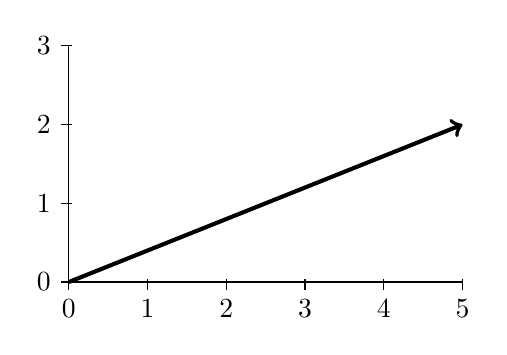
\begin{tikzpicture}
                %axis
                \draw (0,0) -- coordinate (x axis mid) (5,0);
                    \draw (0,0) -- coordinate (y axis mid) (0,3);
                    %ticks
                    \foreach \x in {0,...,5}
                        \draw (\x,1pt) -- (\x,-3pt)
                        node[anchor=north] {\x};
                    \foreach \y in {0,...,3}
                        \draw (1pt,\y) -- (-3pt,\y) 
                        node[anchor=east] {\y};
                \draw   (5,0) -- (0, 0)
                        (0,3) -- (0,0);
                \draw[->,line width=1.5pt] (0,0) -- (5,2);
            \end{tikzpicture}
        
        \end{itemize}

    \item If we multiply by a scalar: $a = 2$, $aX = [10, 4]$
    
    \begin{tikzpicture}
        %axis
        \draw (0,0) -- coordinate (x axis mid) (10,0);
            \draw (0,0) -- coordinate (y axis mid) (0,5);
            %ticks
            \foreach \x in {0,...,10}
                \draw (\x,1pt) -- (\x,-3pt)
                node[anchor=north] {\x};
            \foreach \y in {0,...,5}
                \draw (1pt,\y) -- (-3pt,\y) 
                node[anchor=east] {\y};
        \draw   (10,0) -- (0, 0)
                (0,5) -- (0,0);
        \draw[->,line width=1.5pt] (0,0) -- (5,2);
        \draw[->,line width=1.5pt] (0,0) -- (10,4);
    \end{tikzpicture}

    \end{itemize}
\end{itemize}

\subsubsection{Vector length}

\begin{itemize}
    \item Also called the \emph{norm}, length is not the same as \emph{dimensions}. The formula is:

    \begin{equation*}
        ||x|| = \sqrt{x_1^2 + x_2^2 + ... + x_n^2}
    \end{equation*}

    \item Considering the visuals above, in two dimensions we are just using the Pythagorean theorem. But the formula is extendable to k-dimensions. For $\bm{x} = (5, 2)$, $||\bm{x}|| = \sqrt{25 + 4} = \sqrt{29}$.
    
    \item Another example
    \begin{itemize}
        \item $x = (5,2), y = (1,4)$
        \begin{itemize}
            \item $x + y = (6, 6)$
            \item $||x + y|| = \sqrt{36 + 36} = \sqrt{72}$
        
            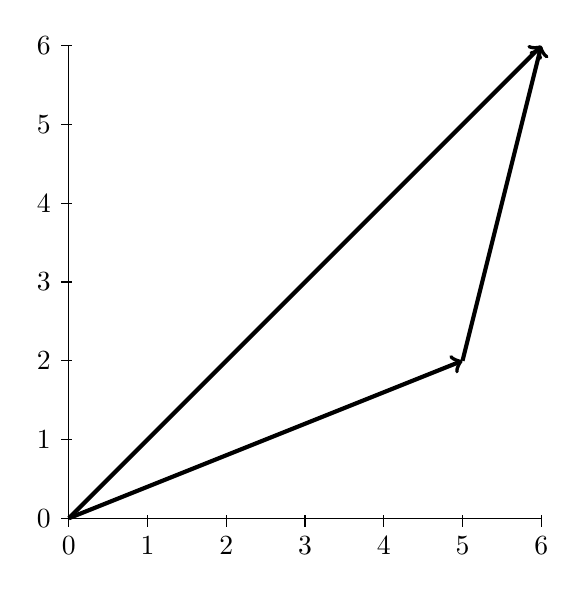
\begin{tikzpicture}
                %axis
                \draw (0,0) -- coordinate (x axis mid) (6,0);
                    \draw (0,0) -- coordinate (y axis mid) (0,6);
                    %ticks
                    \foreach \x in {0,...,6}
                        \draw (\x,1pt) -- (\x,-3pt)
                        node[anchor=north] {\x};
                    \foreach \y in {0,...,6}
                        \draw (1pt,\y) -- (-3pt,\y) 
                        node[anchor=east] {\y};
                \draw   (6,0) -- (0, 0)
                        (0,6) -- (0,0);
                \draw[->,line width=1.5pt] (0,0) -- (5,2);
                \draw[->,line width=1.5pt] (5,2) -- (6,6);
                \draw[->,line width=1.5pt] (0,0) -- (6,6);
            \end{tikzpicture}
        \end{itemize}
    \end{itemize}

    %\item One side note on distance:
    %\begin{itemize}
    %    \item The \emph{triangle inequality} states that:
    %    \begin{itemize}
    %        \item $||x + y|| \leq ||x|| + ||y||$
    %    \end{itemize}
    %\end{itemize}
\end{itemize}

\subsubsection{Vector multiplication}

\begin{itemize}
    \item If $c$ is a \emph{scalar} and we multiply $a(x_1, x_2, ..., x_n)$, then we get $(ax_1, ax_2, ..., ax_n)$. Dividing by a scalar works the same way.
    \item But what about multiplying one vector by another vector? We use the \textbf{dot product}: $\bm{a} \cdot \bm{b}$. Another name for this operation is the \textbf{inner product}.\footnote{For a nice review of vector manipulation, see \url{https://people.cs.clemson.edu/~dhouse/courses/401/notes/vectors.pdf}}
    \begin{itemize}
        \item If $\bm{a}$ and $\bm{b}$ are both n-dimensional, then $\bm{a} \cdot \bm{b} = a_1b_1 + a_2b_2 + ... + a_nb_n = \sum\limits_{i=1}^na_ib_i$
        \begin{equation*}
            \text{Ex: }
            \begin{bmatrix}
                5 \\
                2
            \end{bmatrix} \cdot 
            [1 \; \; 4]
            = (5 \cdot 1) + (2 \cdot 4) = 5 + 8 = 13  
        \end{equation*}
        \item Note: the result of the dot product of vectors is a \emph{scalar}.
    \end{itemize}
    %\item The \textbf{Cauchy-Schwartz inequality} states that $|a \cdot b| %\leq ||a|| \, ||b||$
    \item The \textbf{outer product} of two vectors instead produces a matrix:
    \begin{equation*}
        \begin{bmatrix}
            a_1 \\
            a_2
        \end{bmatrix} \cdot 
        \begin{bmatrix}
            b_1 & b_2
        \end{bmatrix}
        = \begin{bmatrix}
            a_1b_1 & a_1b_2 \\
            a_2b_1 & a_2b_2
        \end{bmatrix}  
    \end{equation*}
    \begin{itemize}
        \item The dimensions of this matrix are the two outer dimensions of the vectors multiplied together:
        \begin{equation*}
            \underset{3 \times 1}{\begin{bmatrix}
                3 \\
                2 \\
                1
            \end{bmatrix}}
            \underset{1 \times 3}{[1 \; \; 2 \; \; 3]} = 
            \underset{3 \times 3}{
            \begin{bmatrix}
                3 & 6 & 9 \\
                2 & 4 & 6 \\
                1 & 2 & 3
            \end{bmatrix}
            }
        \end{equation*}
        \item \emph{But} the inner dimensions must match up. See 1 and 1 above. If the first matrix's number of columns is not equal to the second matrix's number of rows, then cannot multiply.
    \end{itemize}
\end{itemize}

% Take lecture break here
\subsection{Matrices}

\begin{itemize}
    \item A \textbf{matrix} is a rectangular table of numbers or variables arranged in a specific order in rows and columns. We express dimensions by rows, $n$, and columns, $m$. The dimensions of a matrix $A_{n \times m}$ are pronounced `$n$ by $m$'. 
    
    \begin{equation*}
        \bm{X} = 
        \begin{bmatrix}
            x_{11} & x_{12} & x_{13} \\
            x_{21} & x_{22} & x_{23} \\
            x_{31} & x_{32} & x_{33} 
        \end{bmatrix} \in
        \mathbb{R}^{nm} = \mathbb{R}^{3 \times 3}
    \end{equation*}

    \item If $m = n$, then the matrix is symmetric/square.
    
    \item \textbf{Types of matrices}:
    \begin{equation*}
        \begin{bmatrix}
            0 & 0 & 0 \\
            0 & 0 & 0 \\
            0 & 0 & 0
        \end{bmatrix} = \text{zero matrix}
        \; \; \; \;
        \begin{bmatrix}
            1 & 0 & 0 \\
            0 & 2 & 0 \\
            0 & 0 & 3
        \end{bmatrix} = \text{diagonal matrix}
        \; \; \; \; 
        \begin{bmatrix}
            1 & 0 & 0 \\
            0 & 1 & 0 \\
            0 & 0 & 1
        \end{bmatrix} = \text{identity matrix}
    \end{equation*}
\end{itemize}

\subsection{Matrix operators}

\begin{itemize}
    
    \item \textbf{Addition}
    
    \begin{itemize}
        \item Must have the same number of elements
        \begin{equation*}
            \begin{bmatrix}
                1 & 2 & 3 \\
                0 & 0 & 1 \\
                1 & 2 & 1
            \end{bmatrix} +
            \begin{bmatrix}
                1 & 2 \\
                3 & 4 \\
                5 & 6
            \end{bmatrix} = \text{can't do}
        \end{equation*}
        \begin{equation*}
            \begin{bmatrix}
                1 & 2 \\
                0 & 0 \\
                1 & 2
            \end{bmatrix} + 
            \begin{bmatrix}
                1 & 2 \\
                3 & 4 \\
                5 & 6
            \end{bmatrix} =
            \begin{bmatrix}
                2 & 4 \\
                3 & 4 \\
                6 & 8
            \end{bmatrix}
        \end{equation*}
    \end{itemize}

    \item \textbf{Transposition}
    
    \begin{itemize}
        \item Rotate so that the first column becomes the first row:
        \begin{equation*}
            \bm{X} = 
            \underset{3 \times 2}{
            \begin{bmatrix}
                1 & 2 \\
                0 & 0 \\
                1 & 2    
            \end{bmatrix}
            }, 
            \; \; \; 
            \bm{X}^T = 
            \underset{2 \times 3}{
            \begin{bmatrix}
                1 & 0 & 1 \\
                2 & 0 & 2   
            \end{bmatrix}
            }
        \end{equation*}
    \end{itemize} 

    \item \textbf{Multiplication}
        \begin{align*}
            \bm{A} = 
            \begin{bmatrix}
                1 & 2 \\
                3 & 4    
            \end{bmatrix},
            \; \; \; 
            \bm{B} =
            \begin{bmatrix}
                7 & 0 & -1 \\
                1 & 3 & 1
            \end{bmatrix}
        \end{align*}
        
        \begin{itemize}
            \item Because $\bm{A}$ is $2 \times 2$ and $\bm{B}$ is $2 \times 3$, we can multiply. But $\bm{A}\bm{B}^T$ is undefined because $\bm{B}$ is $3 \times 2$. 
        \end{itemize}
        \begin{align*}
            \bm{AB} & =
            \begin{bmatrix}
                1 & 2 \\
                3 & 4
            \end{bmatrix}
            \begin{bmatrix}
                7 & 0 & -1\\
                1 & 3 & 1
            \end{bmatrix} \\
            & = 
            \begin{bmatrix}
                \bm{A}_{11}\bm{B}_{11} + \bm{A}_{12}\bm{B}_{21} & 
                \bm{A}_{11}\bm{B}_{12} + \bm{A}_{12}\bm{B}_{22} &
                \bm{A}_{11}\bm{B}_{13} + \bm{A}_{12}\bm{B}_{23} \\ 
                \bm{A}_{21}\bm{B}_{11} + \bm{A}_{222}\bm{B}_{21} & 
                \bm{A}_{21}\bm{B}_{12} + \bm{A}_{22}\bm{B}_{22} &
                \bm{A}_{21}\bm{B}_{13} + \bm{A}_{22}\bm{B}_{23}
            \end{bmatrix} \\
            & =
            \begin{bmatrix}
                (1 \cdot 7) + (2 \cdot 1) & 
                (1 \cdot 0) + (2 \cdot 3) &
                (1 \cdot -1) + (2 \cdot 1) \\ 
                (3 \cdot 7) + (4 \cdot 1) &
                (3 \cdot 0) + (4 \cdot 3) & 
                (3 \cdot -1) + (4 \cdot 1) 
            \end{bmatrix} 
            = 
            \begin{bmatrix}
                9 & 6 & 1 \\
                29 & 12 & 1
            \end{bmatrix}
        \end{align*}

    \begin{itemize}
        \item Ex with identity matrix:
        \begin{align*}
            \bm{I}_{2 \times 2} \bm{X} & = 
            \begin{bmatrix}
                1 & 0 \\
                0 & 1
            \end{bmatrix}
            \begin{bmatrix}
                1 & 2 \\
                3 & 4
            \end{bmatrix} = 
            \begin{bmatrix}
                1 & 2 \\
                3 & 4
            \end{bmatrix} \\
            & 
            \text{b/c}
            \begin{bmatrix}
                (1 \cdot 1) + (0 \cdot 3) & (0 \cdot 1) + (1 \cdot 2) \\
                (0 \cdot 1) + (1 \cdot 3) & (0 \cdot 3) + (1 \cdot 4) 
            \end{bmatrix}
        \end{align*}
    \end{itemize}

\end{itemize}

\newpage

% Lecture 4: Linear algebra II
\section{Linear Algebra II}

\begin{itemize}

    \item Let's review matrix multiplication once before moving forward:
    \begin{align*}
        \bm{A} = 
        \underset{2 \times 3}{\begin{bmatrix}
            1 & 2 & -3 \\
            4 & 0 & -2   
        \end{bmatrix}},
        \; \; \; 
        \bm{B} =
        \underset{3 \times 2}{\begin{bmatrix}
            3 & 1 \\
            2 & 4 \\
            -1 & 5
        \end{bmatrix}}
    \end{align*}
    
    \item The dimensions of the product of these two matrices is the outside dimensions:
    \begin{align*}
        \bm{A}\bm{B} & = (\bm{2} \times 3) \cdot (3 \times \bm{2}) = 2 \times 2 \\ 
        \bm{B}\bm{A} & = (\bm{3} \times 2) \cdot (2 \times \bm{3}) = 3 \times 3
    \end{align*}

    \item We know we can multiply the two together in either direction because the inner dimensions match in either order.
    \begin{align*}
        \begin{bmatrix}
            1 & 2 & -3 \\
            4 & 0 & 2
        \end{bmatrix}
        \begin{bmatrix}
            3 & 1 \\
            2 & 4 \\
            -1 & 5
        \end{bmatrix}
        = 
        \begin{bmatrix}
            3 + 4 + 3 & 1 + 8 -15 \\
            12 + 0 -2 & 4 + 0 + 10
        \end{bmatrix}
        = 
        \begin{bmatrix}
            10 & -6 \\
            10 & 14
        \end{bmatrix}
    \end{align*}

    \item One more example:
    \begin{align*}
        \begin{bmatrix}
            1 & 2 & 1 \\
            0 & 1 & 1
        \end{bmatrix}
        \begin{bmatrix}
            4 & 3 \\
            7 & 8 \\
            1 & 2
        \end{bmatrix} 
        = 
        \begin{bmatrix}
            4 + 14 + 1 & 3 + 16 + 2 \\
            0 + 7 + 1 & 0 + 8 + 2 
        \end{bmatrix}
        = 
        \begin{bmatrix}
            19 & 21 \\
            8 & 10
        \end{bmatrix}
    \end{align*}
\end{itemize}


\subsection{Matrix Representation of Systems of Equations}

\begin{itemize}
    \item Take this system of equations:
    \begin{align*}
        a_{11}x_1 + a_{12}x_2 + ... + a_{1n}x_n & = b_1 \\
        \vdots & \\
        a_{m1}x_1 + a_{m2}x_2 + ... + a_{mn}x_n & = b_m 
    \end{align*}

    \item Or in matrix form:
    \begin{align*}
        \underset{m \times n}{
            \begin{bmatrix}
                a_{11} & a_{12} & ... & a_{1n} \\
                \vdots & \\
                a_{m1} & a_{m2} & ... & a_{mn}
            \end{bmatrix}
        }
        \underset{n \times 1}{
            \begin{bmatrix}
                x_1 \\
                x_2 \\
                \vdots \\
                x_n
            \end{bmatrix}
        }
        =
        \underset{m \times 1}{
            \begin{bmatrix}
                b_1 \\
                b_2 \\
                \vdots \\
                b_m
            \end{bmatrix}
        }
    \end{align*}

    \item Ex:
    \begin{align*}
            2x_1 + 3x_2 - 1x_3 & = 7 \\
            4x_1 + 5x_2 + 6x_3 & = 8 \\
            -1x_1 + 2x_2 + 1x_3 & = 9    
    \end{align*}
    \vspace{-3.5em}
    \begin{center}
        $\Downarrow$
    \end{center}
    \vspace{-2em}
    \begin{align*}
        \underset{A}{
            \begin{bmatrix}
                2 & 3 & -1 \\
                4 & 5 & 6 \\
                -1 & 2 & 1
            \end{bmatrix}
        }
        \underset{X}{
            \begin{bmatrix}
                x_1 \\
                x_2 \\
                x_3
            \end{bmatrix}
        }
        =
        \underset{b}{
            \begin{bmatrix}
                7 \\
                8 \\
                9
            \end{bmatrix}
        }
    \end{align*}
\end{itemize}


\subsection{Linear Dependence and Independence}

\begin{itemize}
    \item The \textbf{span} of a vector is all of its linear combinations. I.e. $c\begin{bmatrix} 2 \\ 3 \end{bmatrix} \forall \, c$.
    \begin{itemize}
        \item On linear combinations: the linear combination of 
        \vspace{-1em}
        \begin{align*}
            2x \\
            3x
        \end{align*}

        \vspace{-2em}
        is $x \begin{bmatrix}
            2 \\ 3 
        \end{bmatrix}$
    \end{itemize}
    \item If one vector falls in the span of another vector then the two are \textbf{linearly dependent}. There is no new information in the second vector.
    \begin{itemize}
        \item $ \begin{bmatrix} 2 \\ 3 \end{bmatrix}$ and 
            $\begin{bmatrix} 4 \\ 6 \end{bmatrix}$ are linearly dependent. The second is the first times 2. 
    \end{itemize}
    \item If one vector \emph{does not} fall in the span of another vector, then the two are \textbf{linearly independent}.
    \begin{itemize}
        \item $\begin{bmatrix} 7 \\ 0\end{bmatrix}$ and 
        $\begin{bmatrix} 0 \\ -1 \end{bmatrix}$ are linearly independent. One cannot be represented as a linear combination of the other.
    \end{itemize}
    \item If we were to draw each item in the vector set, then we are interested in whether or not the overall span of a set changes when a vector is added or removed. 
    %\item Formally, a vector set is linearly independent if, for a set $S = \{\bm{v}_1, \bm{v}_2, ..., \bm{v}_n\}$ the only solution to $c_1\bm{v}_1 + c_2\bm{v}_2 + ... + c_n\bm{v}_n = 0$ is $c_1 = c_2 = ... = c_n = 0$.
    %\begin{itemize}
    %    \item If, on the other hand, at least one solution includes a non-zero scalar, then the vector set is linearly dependent.
    %\end{itemize}
\end{itemize}

\subsection{Properties of Matrix Operators}

\begin{itemize}
    
    \item Matrix Addition
    \begin{itemize}
        \item If $\bm{A}$ and $\bm{B}$ are both the same size ($m \times n$):
        \begin{enumerate}
            \item $\bm{A} + \bm{B} = \bm{B} + \bm{A}$
            \item $\bm{A} + (\bm{B} + \bm{C}) = (\bm{A} + \bm{B}) + \bm{C}$
            \item Additive Inverse: $\bm{A} + (- \bm{A}) = 0_{m \times n}$  
        \end{enumerate}
    \end{itemize}

    \item Matrix Multiplication:
    \begin{itemize}
        \item If $\bm{A}, \bm{B}, \bm{C}$ are conformable:
        \begin{enumerate}
            \item $\bm{A}(\bm{B}\bm{C}) = (\bm{A}\bm{B})\bm{C}$
            \item $\bm{I}\bm{A} = \bm{A}\bm{I} = \bm{A}$
            \begin{itemize}
                \item Where $\bm{I}$ is an identity matrix, e.g. $\bm{I}_{3 \times 3} = 
                \begin{bmatrix}
                    1 & 0 & 0 \\
                    0 & 1 & 0 \\
                    0 & 0 & 1    
                \end{bmatrix}$
            \end{itemize}
            \item $\bm{A}(\bm{B} + \bm{C}) = \bm{AB} + \bm{AC} \neq \bm{BA} + \bm{CA}$ because order matters
        \end{enumerate}
    \end{itemize}

    \item Matrix Exponents
    \begin{enumerate}
        \item $\bm{A}^p \cdot \bm{A}^q = \bm{A}^{p + q}$
        \item $(\bm{A}^p)^q = \bm{A}^{pq}$ 
        \item $(\bm{A}\bm{B})^p \neq \bm{A}^p\bm{B}^p$ unless $\bm{AB} = \bm{BA}$
    \end{enumerate}
    
    \item Scalar Multiplication; $\bm{A}, \bm{B}$ are matrices and $r, s$ are scalars:
    \begin{enumerate}
        \item $r(s\bm{A}) = (rs\bm{A})$
        \item $(r + s)\bm{A} = r\bm{A} + s\bm{A}$
        \item $r(\bm{A} + \bm{B}) = r\bm{A} + r\bm{B}$
        \item $A(r\bm{B}) = r\bm{A}\bm{B} = \bm{A}\bm{B}r$
    \end{enumerate}

    \item Matrix Transposition
    \begin{enumerate}
        \item $(\bm{A}^T)^T = \bm{A}$
        \item $(\bm{A} + \bm{B})^T = \bm{A}^T + \bm{B}^T$
        \item $(\bm{AB})^T = \bm{B}^T\bm{A}^T$
        \item $(rA)^T = r(A^T)$
    \end{enumerate}

    \item Symmetric Matrix: A square matrix is symmetric if $\bm{A}^T = \bm{A}$
    \begin{itemize}
        \item Ex: $
            \begin{bmatrix}
                1 & 2 & 3 \\
                2 & 4 & 1 \\
                3 & 1 & 5
            \end{bmatrix}
            $
    \end{itemize} 
\end{itemize}


\subsection{Idempotent Matrices}

\begin{itemize}
    \item A matrix, $\bm{A}$, is idempotent if $\bm{AA} = \bm{A}$. Multiplying the matrix by itself returns the original matrix.
\end{itemize}


\subsection{Reduced Row/Row Echelon Form and Solving Linear Systems of Equations Gauss-Jordan Reduction/Elimination}


\begin{itemize}
    \item We can use a matrix to represent a system of equations:
    \begin{align*}
        a_{11}x_1 + a_{12}x_2 + ... + a_{1n}x_n & = b_1 \\
        a_{21}x_1 + a_{22}x_2 + ... + a_{2n}x_n & = b_2 \\
                                                & \vdots \\
        a_{m1}x_1 + a_{m2}x_2 + ... + a_{mn}x_n & = b_m 
    \end{align*}    
    \item Rewritten as an \textbf{augmented matrix}:
    
    \begin{center}
    $\begin{bmatrix}[cccc|c]
        a_{11} & a_{12} & ... & a_{1n} & b_1 \\
        a_{21} & a_{22} & ... & a_{2n} & b_2 \\
        \vdots &        & \ddots & \vdots & \vdots \\
        a_{m1} & a_{m2} & ... & a_{mn} & b_m
    \end{bmatrix}$
    \end{center} 

    \item To solve for a system of equations, we often want to translate a matrix into \textbf{row echelon} or \textbf{reduced row echelon} form.  What conditions describe a matrix in row echelon and reduced row echelon form. The conditions are:
    \begin{enumerate}
        \item If any rows are zeros, then they are below nonzero rows (include at least one nonzero element): 
            
        $\begin{bmatrix}[ccc|c]
            1 & 2 & 3 & 7 \\
            0 & 0 & 0 & 0 
        \end{bmatrix}$
        
        \item The first non-zero entry in any row is 1 (except all zero row).
            
        $\begin{bmatrix}[ccc|c]
            0 & 1 & 3 & 7 \\
            0 & 0 & 0 & 0 
        \end{bmatrix}$
            
        \item For each non-zero row the leading 1 is to the right of each 1 in the row above.
            
        $\begin{bmatrix}[ccc|c]
            1 & 0 & 3 & 7 \\
            0 & 1 & 4 & 0 \\
            0 & 0 & 1 & 2 
        \end{bmatrix}$
            
        \item \textbf{Reduced row-echelon form}: makes the solution to a system of equations obvious. Below $x_1 = 7, x_2 = 0, x_3 = 2$
        
        $\begin{bmatrix}[ccc|c]
            1 & 0 & 0 & 7 \\
            0 & 1 & 0 & 0 \\
            0 & 0 & 1 & 2
        \end{bmatrix}$

    \end{enumerate}

    \item Transforming a matrix into row echelon and reduced row echelon form is referred to as \textbf{Gauss-Jordan elimination}. We do so through \textbf{elementary row operators}:
    
    \begin{itemize}
        \item Multiplying a row by a constant
        \begin{itemize}
            \item Remember, the matrix is a system of equations. So we're just multiplying both sides of an equation.
        \end{itemize}
        \item Adding/subtracting rows
        \item Interchanging rows
    \end{itemize}
    
    \item Example:
    \begin{align*}
        1x_1 + 2x_2 + 4x_3 & = 3 \\
        2x_1 + 1x_2 + 3x_3 & = 2 \\
        1x_1 + 2x_2 + 2x_3 & = 3
    \end{align*}

    \begin{itemize}
        \item As an augmented matrix:

        \begin{center}
            $\begin{bmatrix}[ccc|c]
                1 & 2 & 4 & 3 \\
                2 & 1 & 3 & 2 \\
                1 & -2 & 2 & 3
            \end{bmatrix}$    
        \end{center}

        \item Add $-2r1$ to $r2$ and $-1r1$ to $r3$

        \begin{center}
            $\begin{bmatrix}[ccc|c]
                1 & 2 & 4 & 3 \\
                0 & -3 & -5 & -4 \\
                0 & -4 & -2 & 0
            \end{bmatrix}$    
        \end{center}

        \item $r3 \times -\frac{1}{4}$ and interchange $r2$ and $r3$
        
        \begin{center}
            $\begin{bmatrix}[ccc|c]
                1 & 2 & 4 & 3 \\
                0 & 1 & 1/2 & 0 \\
                0 & -3 & -5 & -4
            \end{bmatrix}$
        \end{center}

        \item Add $3r2$ to $r3$ 

        \begin{center}
            $\begin{bmatrix}[ccc|c]
                1 & 2 & 4 & 3 \\
                0 & 1 & 1/2 & 0 \\
                0 & 0 & -7/2 & -4
            \end{bmatrix}$
        \end{center}

        \item Multiply $r3$ by $-\frac{2}{7}$

        \begin{center}
            $\begin{bmatrix}[ccc|c]
                1 & 2 & 4 & 3 \\
                0 & 1 & 1/2 & 0 \\
                0 & 0 & 1 & 8/7
            \end{bmatrix}$
        \end{center}

        \item Subtract $4r3$ from $r1$ and subtract $\frac{1}{2}r3$ from $r2$
        
        \begin{center}
            $\begin{bmatrix}[ccc|c]
                1 & 2 & 0 & -11/7 \\
                0 & 1 & 0 & -4/7 \\
                0 & 0 & 1 & 8/7
            \end{bmatrix}$
        \end{center}

        \item Subtract $2r2$ from $r1$
    
        \begin{center}
            $\begin{bmatrix}[ccc|c]
                1 & 0 & 0 & -3/7 \\
                0 & 1 & 0 & -4/7 \\
                0 & 0 & 1 & 8/7
            \end{bmatrix}$
        \end{center}

        \item $x_1 = -\frac{3}{7}, x_2 = -\frac{4}{7}, x_3 = \frac{8}{7}$ 
        \item Or: $\text{I}_3X = \begin{bmatrix}
            -3/7 \\ -4/7 \\ 8/7
        \end{bmatrix}$

    \end{itemize}
\end{itemize}

\newpage 

% Lecture 5: Linear algebra III
\section{Linear Algebra III}

\subsection{Matrix Inversion}

\begin{itemize}
    \item For a scalar $a$, the inverse: $a^{-1} = \frac{1}{a}$, where $a^{-1}a = 1$.
    \item We can also invert a matrix $A$: $A^{-1}A = AA^{-1} = \text{I}$
    \begin{itemize}
        \item Note: if $A^{-1}$ does not exist, then $A$ is singular/not invertible.
        \item $A^T \neq A^{-1}$
    \end{itemize}
    \item For a $2 \times 2$ matrix, we use the following steps. We'll cover larger matrices after, for which we'll use a lengthier, but more intuitive process.
    \begin{align*}
        A & = \begin{bmatrix}
            a & b \\
            c & d 
        \end{bmatrix} \\
        A^{-1} & = \frac{1}{ad - bc} 
        \begin{bmatrix}
            d & -b \\
            -c & a 
        \end{bmatrix}
    \end{align*}

    Where $\frac{1}{ad - bc}$ is the \emph{determinant}, which we discuss more later. An example:

    \begin{align*}
        A & = \begin{bmatrix}
            1 & 2 \\
            3 & 4 
        \end{bmatrix} \\
        A^{-1} & = \frac{1}{(1\cdot4) - (3 \cdot 2)} 
        \begin{bmatrix}
            4 & -2 \\
            -3 & 1 
        \end{bmatrix} \\
        & = \frac{1}{-2} 
        \begin{bmatrix}
            4 & -2 \\
            -3 & 1
        \end{bmatrix} = 
        \begin{bmatrix}
            -2 & 1 \\
            3/2 & -\frac{1}{2}
        \end{bmatrix}
    \end{align*}
    
    \item How to check if $A^{-1}A = \text{I}$?
    \begin{equation*}
        \begin{bmatrix}
            -2 & 1 \\
            3/2 & -1/2
        \end{bmatrix}
        \begin{bmatrix}
            1 & 2 \\
            3 & 4
        \end{bmatrix}
        = 
        \begin{bmatrix}
            1 & 0 \\
            0 & 1
        \end{bmatrix}
    \end{equation*}
\end{itemize}

\subsection{Properties of Matrix Inversion}

Singular vs nonsingular:

\begin{itemize}
    \item Invertible = Nonsingular
    \item Noninvertible = Singular
    \item If $A$ is nonsingular, then $A^{-1}$ is nonsingular
    \item If $A$ \& $B$ are nonsingular, then $(AB)^{-1} = B^{-1}A^{-1}$
    \item If $A$ is nonsingular, then $(A^T)^{-1} = (A^{-1})^T$
\end{itemize}

\noindent Some conditions for nonsingularity (we can find $A^{-1}$, there are often more conditions listed, but they are technically covered by these three):

\begin{enumerate}
    \item Rows and columns are linearly independent
    \begin{itemize}
        \item No rows and/or columns add up to each other. Generally speaking if rows and columns are not linearly independent, then the matrix is invertible.
    \end{itemize}
    \item Matrix $A$ is row equivalent to $I$ (can we use row operators to turn $A$ into the identity matrix?)
    % \item $n \times n$ matrix $A$ is of rank $n$ (number of linearly independent rows and columns, equivalent to condition 1)
    \item The determinant (we cover below) is not 0.
    %\item $\forall$ (``for all'') vectors $b$, $\exists !$ (there exists a unique solution) to $Ax = b$ 
\end{enumerate}

\noindent One intuitive and practical procedure for finding $A^{-1}$, regardless of the size:

\begin{enumerate}
    \item Find $[A|\text{I}]$ where both $A$ and I are both $n \times n$
    \item Find the reduced row echelon form for A (left side)
    \item If step 2 gives us $[\text{I}|C]$, then $C = A^{-1}$
\end{enumerate}

\noindent A note on rank: If $A$ is $m \times n$, then the rank($A$) = 
\[ \text{min} \begin{cases} 
    \text{max \# of linearly ind. rows} \\
    \text{max \# of linearly ind. cols} 
\end{cases}
\]

\begin{itemize}
    \item E.g.: 
    $\begin{bmatrix}
        \bm{1} & \bm{2} & \bm{3} \\
        \bm{1} & 2 & 3 \\
        \bm{2} & 4 & 6
    \end{bmatrix}$ Only the bold rows and columns are linearly ind. So, rank$(A) =$ min$(1,1) = 1$
\end{itemize}

\begin{itemize}
    \item \textbf{Examples:}

    $
    \bm{A}\text{I} = 
    \begin{bmatrix}[ccc|ccc]
        1 & 1 & 1 & 1 & 0 & 0 \\
        0 & 2 & 3 & 0 & 1 & 0 \\
        5 & 5 & 1 & 0 & 0 & 1
    \end{bmatrix}
    $

    \begin{itemize}
        \item Subtract 1/2 r2 from r1, divide r2 by 2, subtract 5r1 from r3
    \end{itemize}

    $
    = \begin{bmatrix}[ccc|ccc]
        1 & 0 & -1/2 & 1 & - 1/2 & 0 \\
        0 & 1 & 3/2 & 0 & 1/2 & 0 \\
        0 & 0 &  4 & -5 & 0 & 1
    \end{bmatrix}
    $

    \begin{itemize}
        \item Subtract 1/8r3 from r1, add 3/8r3 to r2, divide r3 by -4
    \end{itemize}

    $
    = \begin{bmatrix}[ccc|ccc]
        1 & 0 & 0 & 13/8 & -1/2 & -1/8 \\
        0 & 1 & 0 & 15/8 & 1/2 & 3/8 \\
        0 & 0 & 1 & 5/4 & 0 & -1/4 
    \end{bmatrix}
    $

    \begin{itemize}
        \item Where the right-hand side matrix is $A^{-1}$
    \end{itemize}

    \item Another example, but $A^{-1}$ doesn't exist:

    $\begin{bmatrix}[ccc|ccc]
        1 & 2 & -3 & 1 & 0 & 0 \\
        1 & -2 & 1 & 0 & 1 & 0 \\
        5 & -2 & -3 & 0 & 0 & 1
    \end{bmatrix}$

    \begin{itemize}
        \item Subtract r1 from r2, subtract 5r1 from r3
    \end{itemize}

    $\begin{bmatrix}
        1 & 2 & 3 & ... & ... & ... \\
        0 & -4 & 4 & ... & ... & ... \\
        0 & -12 & 12 & ... & ... & ...
    \end{bmatrix}$

    \begin{itemize}
        \item We aren't concerned with the right-hand side matrix because the rows of the left matrix are not independent. r3 is a linear combination of r2, meaning the matrix is singular... 
    \end{itemize}

\end{itemize}

\subsection{Determinant}

\begin{itemize}
    \item Determinants convert a matrix into a scalar but can only be defined for a square matrix. Determinants are useful for checking if a matrix is invertible. They also can play a role in solving for systems of equations. The formula is straightforward for a $2 \times 2$ matrix, but less so for larger matrices. 
    \item Let 
    $A = 
    \begin{vmatrix}
        a_{11} & a_{12} \\
        a_{21} & a_{22}
    \end{vmatrix}
    \begin{bmatrix}
        a_{11} & a_{12} \\
        a_{21} & a_{22}
    \end{bmatrix}$
    \begin{itemize}
        \item The determinant of $A$ is the two diagonal products differenced:
        
        $|A| = (a_{11} \cdot a_{22}) - (a_{21} \cdot a_{12})$
    \end{itemize}
    \item Examples:
    \begin{itemize}
        \item $\begin{bmatrix}
            2 & 3 \\ 
            1 & 5 
        \end{bmatrix} 
        \Rightarrow 
        (2 \cdot 5) - (3 \cdot 1) = 7$
        \item  $\begin{bmatrix}
            1 & 1 \\
            2 & 2 
        \end{bmatrix} 
        \Rightarrow 
        2 - 2  = 0$
    \end{itemize}

    \item For a $3 \times 3$ matrix we sum the products of all elements in any row or column, alternating signs, and the determinants of a specific $2 \times 2$ submatrix. An element's submatrix is the remaining elements when the elements from the relevant row and column are removed. I.e., for:
    
    $A = \begin{bmatrix}
        a_{11} & a_{12} & a_{13} \\
        a_{21} & a_{22} & a_{23} \\
        a_{31} & a_{32} & a_{33} 
    \end{bmatrix}$

    The submatrix for $a_{23}$ is 
    $\begin{bmatrix}
        a_{11} & a_{12} \\
        a_{31} & a_{32}    
    \end{bmatrix}$ 

    Taking the first column, the determinant of $A$ is:

    $
    a_{11}
    \begin{vmatrix}
        a_{22} & a_{23} \\
        a_{32} & a_{33}    
    \end{vmatrix}
    - a_{21}
    \begin{vmatrix}
        a_{12} & a_{13} \\
        a_{32} & a_{33}
    \end{vmatrix}
    + a_{31}
    \begin{vmatrix}
        a_{12} & a_{13} \\
        a_{22} & a_{23}
    \end{vmatrix}
    $

    \item We can use any row or column. But it is best to use one with zeros, if available. 

    \item The \textbf{minor} of an element is the determinant of its submatrix.
    \begin{itemize}
        \item $M_{12} = 
        \begin{vmatrix}
            a_{21} & a_{23} \\
            a_{31} & a_{33}
        \end{vmatrix}
        =
        (a_{21} \cdot a_{33}) - (a_{31} \cdot a_{23})
        $
    \end{itemize}
\end{itemize}

\subsubsection{Determinants via Cofactor Expansion}

\begin{itemize}
    \item The \textbf{cofactor} of any element $i,j$: $C_{ij} = (-1)^{i + j}M_{ij}$, which is used for calculating the determinants of $n \times n$ matrices where $n > 2$.  $i$ is rows, $j$ is columns.
    \begin{itemize}
        \item $
        A = \begin{bmatrix}
            a_{11} & a_{12} & a_{13} \\
            a_{21} & a_{22} & a_{23} \\
            a_{31} & a_{32} & a_{33}
        \end{bmatrix} 
        $
        \item Ex: $C_{11} = (-1)^{1 + 1} \, \, M_{11} = 1\begin{vmatrix}
            a_{22} & a_{23} \\
            a_{32} & a_{33}
        \end{vmatrix}$
    \end{itemize} 
    \item The determinant of a $n \times n$ matrix where $n >2$ is the sum of the products of each element and its cofactor for any row or column. We just choose a single row or a single column -- ideally one with as many zeros as possible.
    \begin{itemize}
        \item Given row $i$:
        \begin{equation*}
            \text{det}(A) = \sum_{j = 1}^n a_{ij}C_{ij}
        \end{equation*}
        \item Or row $j$:
        \begin{equation*}
            \text{det}(A) = \sum_{i = 1}^n a_{ij}C_{ij}
        \end{equation*}
    \end{itemize}
    \item Let's show what this means:
    \item Choose the row or column with the most zeros:
    \begin{itemize}
        \item Ex: $\begin{bmatrix}
            1 & 2 & -3 & 4 \\
            -4 & 2 & 1 & 3 \\
            0 & 0 & 0 & -3 \\
            2 & 0 & -2 & 3
        \end{bmatrix}$
        \item So let's take all elements in row 3, multiply each times its cofactor, and add it all together. Because of the zeros, we only have to find one cofactor! 
        
        \begin{align*}
            |A| = \sum_{j=1}^4 a_{3j}C_{3j} & = a_{31}C_{31} + a_{32}C_{32} + a_{33}C_{33} + a_{34}C_{34} \\
            a_{34}C_{34} & = 0 + 0 + 0 + a_{34}C_{34} \\
            a_{34}C_{34} & = -3\left[(-1)^{3+4}
            \begin{vmatrix}
                1 & 2 & -3 \\
                -4 & 2 & 1 \\
                2 & 0 & 2
            \end{vmatrix}  
            \right] \\ 
            & = -3 \cdot -1 \left[2 
            \begin{vmatrix}
                2 & -3 \\
                2 & 1    
            \end{vmatrix} - 0 
            \begin{bmatrix}
                1 & -3 \\
                -4 & 1
            \end{bmatrix} + (-2)
            \begin{vmatrix}
                1 & 2 \\
                -4 & 2
            \end{vmatrix}
            \right] \\
            & = 3 \left[2(2 + 6) - 2(2+8) \right] \\
            & = 3[16 - 20] = 3(-4) = -12
        \end{align*}
    \end{itemize}
\end{itemize}

\begin{itemize}
    \item To wrap up, some useful properties of determinants:
    \begin{enumerate}
        \item $|A| = |A^T|$
        \item If a row or column of A is a linear combination of other rows or columns, then $\text{det}(A) = 0$
        \item If $A$ is diagonal, then $|A|$ is the product of the diagonals.
        \item $|AB| = |A| \cdot |B|$
        \item If $A$ is non-singular, then $|A^{-1}| = \frac{1}{|A|}$
    \end{enumerate}
\end{itemize}

\subsection{Adjoint Matrix}

\begin{itemize}
    \item \textbf{Adjoint matrix}: the transpose of a matrix of the cofactors of each element:
    
    \begin{equation*}
        \text{adj}(A) = 
        \begin{bmatrix}
            c_{11} & c_{12} & ...  & c_{1n} \\
            c_{21} & ... & ... & c_{2n} \\
            \vdots & & & \\
            c_{n1} & ... & ...  & c_{nn}     
        \end{bmatrix}
    \end{equation*}

    Where $c$ is an element's cofactor. For example:

    $
    A = \begin{bmatrix}
        1 & 2 & 3 \\
        4 & 5 & 6 \\
        7 & 8 & 9
    \end{bmatrix}
    \Rightarrow 
    C = 
    \begin{bmatrix}
        + \begin{vmatrix}
            5 & 6 \\
            8 & 9
        \end{vmatrix} & 
        - \begin{vmatrix}
            4 & 6 \\
            7 & 9 
        \end{vmatrix} & 
        + \begin{vmatrix}
            4 & 5 \\
            7 & 8
        \end{vmatrix} \\ \\
        - \begin{vmatrix}
            2 & 3 \\
            8 & 9 
        \end{vmatrix} &
        + \begin{vmatrix}
            1 & 3 \\
            7 & 9
        \end{vmatrix} & 
        - \begin{vmatrix}
            1 & 2 \\
            7 & 8
        \end{vmatrix} \\ \\ 
        + \begin{vmatrix}
            2 & 3 \\
            5 & 6
        \end{vmatrix} & 
        - \begin{vmatrix}
            1 & 3 \\
            4 & 6
        \end{vmatrix} & 
        + \begin{vmatrix}
            1 & 2 \\
            4 & 5
        \end{vmatrix}
    \end{bmatrix}
    = 
    \begin{bmatrix}
        -3 & 6 & -3 \\
        6 & -12 & 6 \\
        -3 & 6 & -3
    \end{bmatrix}
    $

    Where the last matrix is the adjoint matrix. 
    
    This information gives us another way to calculate the inverse of $A$ with the following formula: 

    \begin{equation*}
        A^{-1} = \frac{\text{adj}^T}{|A|}
    \end{equation*}

\end{itemize}



\subsection{Trace}

Let's close with something simpler. The \textbf{trace} of a $n \times n$ matrix is just the sum of the diagonal elements.

\begin{equation*}
    \text{Tr} (A) = \Sigma_{i=1}^n a_{11} = a_{11} + a_{22} + ... + a_{nn}
\end{equation*}

\noindent This is less frequently used, but worth being aware of.

\newpage

% Lecture 6: Calculus I
\section{Calculus I}

Before we begin introducing mathematical formula, what is a derivative? A derivative calculates the rate of change of a function at any given point. In high school when we learned about the slope of a line -- $y = mx + b$, where $m$ is the slope -- that slope is a derivative. In that context, the derivative is the same at all points because the line is straight. But we often encounter functions that are not a straight line and we care about calculating the slope across values of that function. We can use calculus for this.


\subsection{Sequences and Limits}

A sequence is an ordered list of numbers, e.g.
\begin{equation*}
    \{x_n\} = \{x_1, x_2, ..., x_n\}
\end{equation*}

\noindent Where $x_n$ is a real number that extends from $x_1$ to $x_n$. We usually encounter $n$ extending to $\infty$. Another way to write the series is:
\begin{equation*}
    \{x_n\}_{n=1}^\infty
\end{equation*}

\noindent Central to calculus is the notion of a sequence ``converging to a limit'', generally where $n \rightarrow \infty$ or $n \rightarrow 0$. This is written as:
\begin{equation*}
    \lim_{n \rightarrow \infty} y_n = L
\end{equation*}

\noindent where L is the limit. Let's visualize for an arbitrary function, $f(x) = \frac{x + 10}{x}$:

\begin{center}
    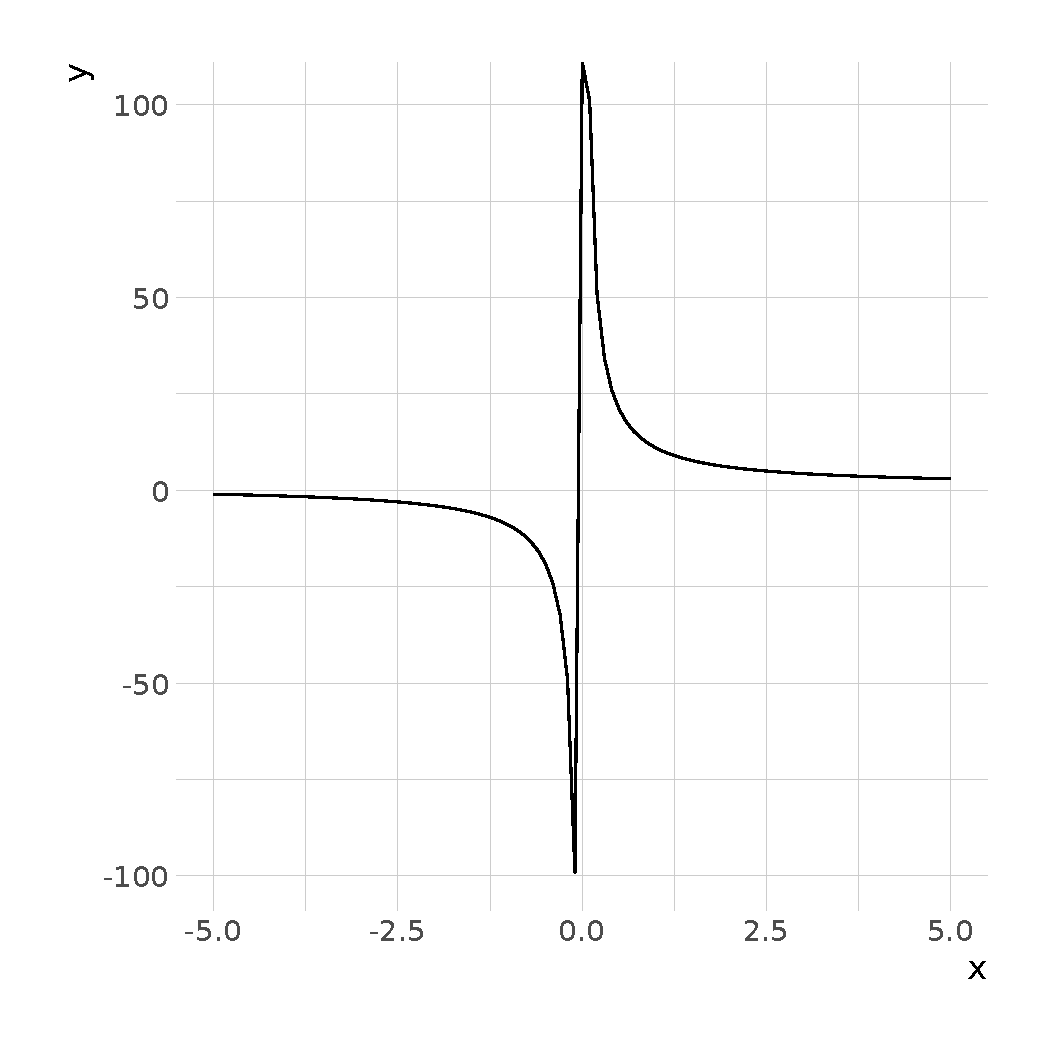
\includegraphics[scale = 0.55]{figures/limit.pdf}    
\end{center}

\noindent We can see that as $x \rightarrow \infty$ the value of $f(x)$ stabilizes. Indeed:

\begin{equation*}
    \lim_{x \rightarrow \infty} \frac{x + 10}{x} = 
    \lim_{x \rightarrow \infty} \left(1 + \frac{10}{x}\right) = 
    \underbrace{\lim_{x \rightarrow \infty} 1}_1 + \underbrace{\lim_{x \rightarrow \infty} \frac{10}{x}}_0 = 1
\end{equation*}

\noindent This gives us a limit of 1.

\subsection{Derivatives and the Difference Quotient}

The derivative is the rate of change of $f(x)$ at any $x$. For a straight line, i.e $y = mx + b$, the derivative is constant at all points. But for a nonlinear function, i.e. $y = 2x^4$, the rate of change varies across x.

\begin{figure}[ht]
    \centering
        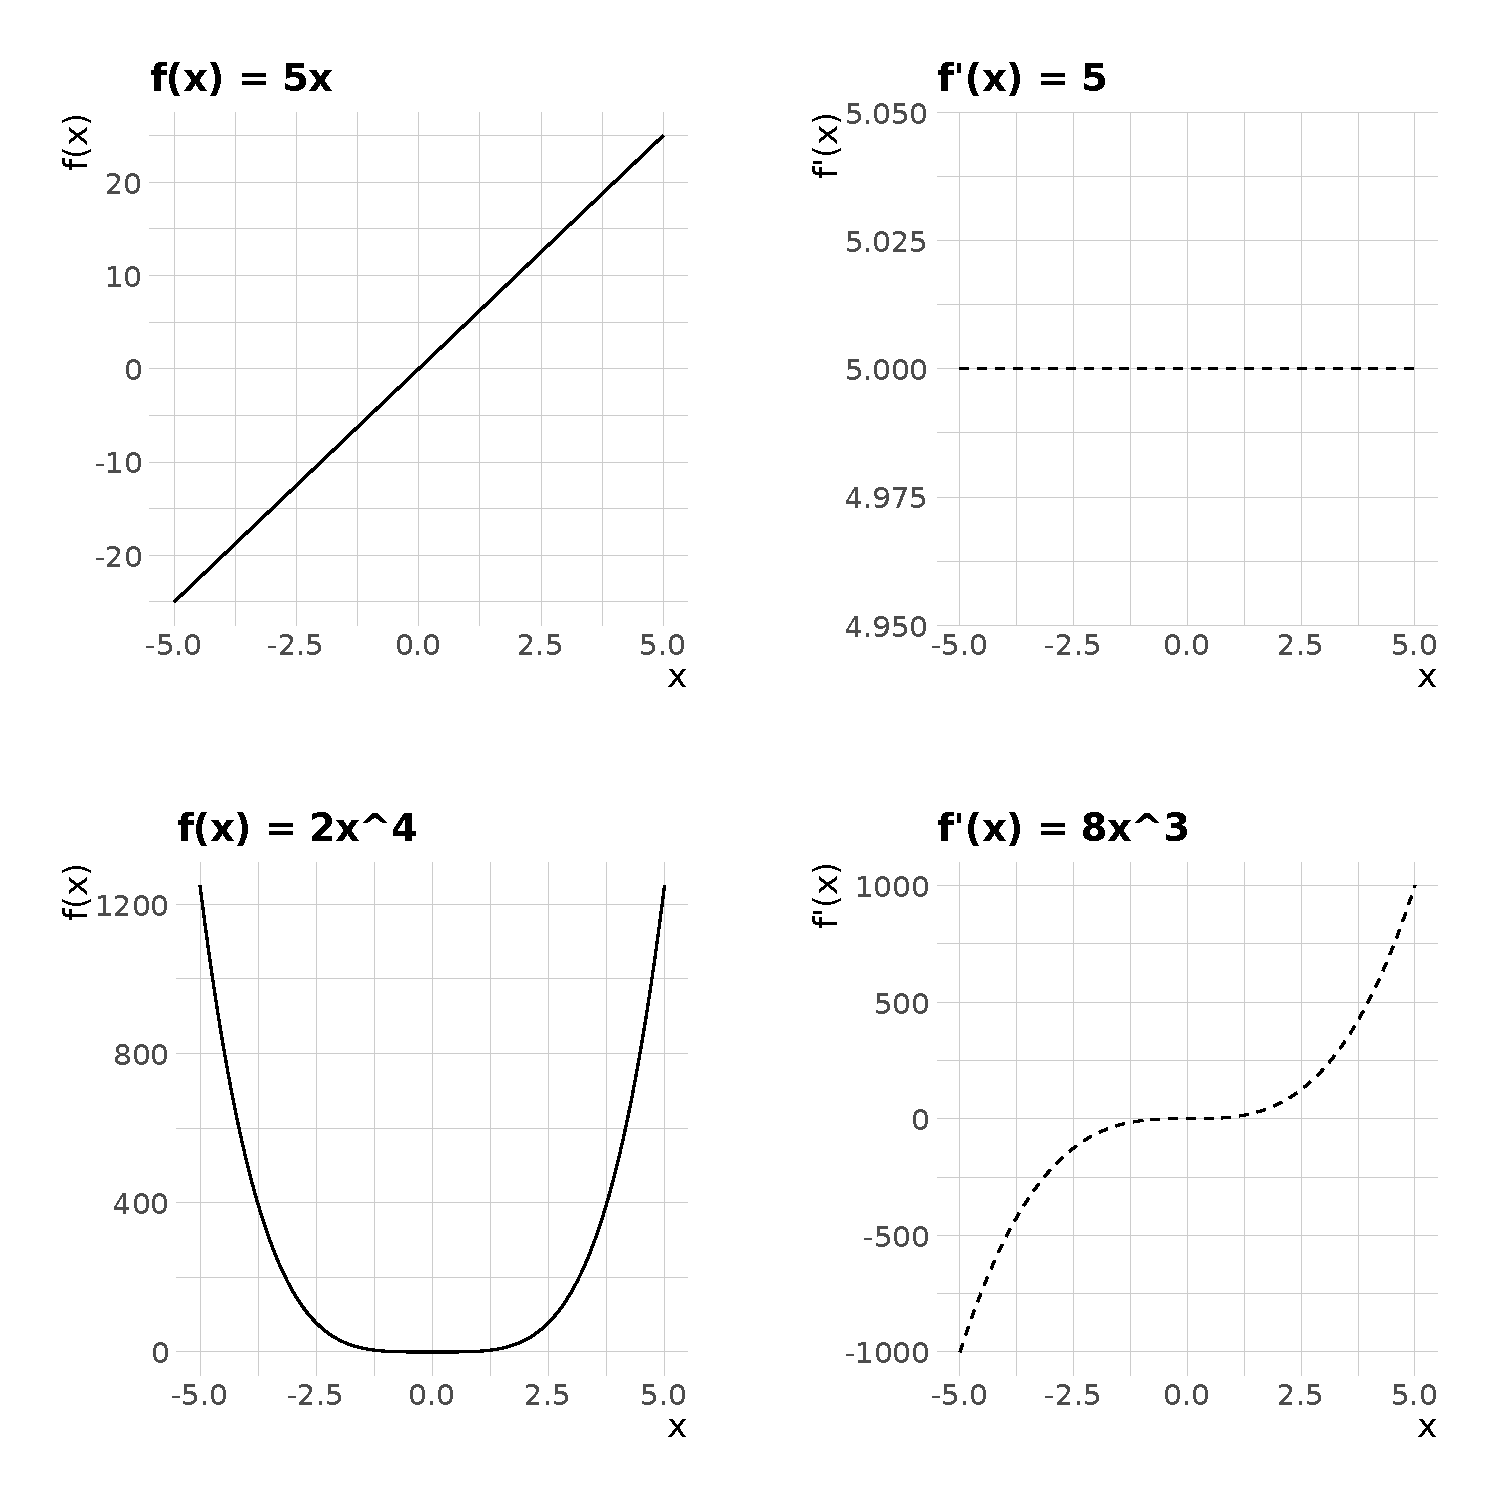
\includegraphics[scale = 0.55]{figures/derivs.pdf}    
    \caption{Functions and their derivatives}
    \label{fig:deriv}
\end{figure}

\noindent Now, let's introduce how we produce a derivative. Let $f$ be a function with an open interval that contains $x$. Let $h$ be the interval where $f(x)$ changes. Below we are simply calculating rise over run at each specified interval.

\begin{equation*}
    \frac{d}{dx}f(x) = 
    \lim_{\Delta x \rightarrow 0} \frac{f(x + \Delta x) - f(x)}{\Delta x} 
\end{equation*}

\noindent The numerator represents the change in $f(x)$ as $\Delta x$ approaches 0 and the denominator is the change in $\Delta x$ -- or the change in $x$. We generally see two notations for derivatives:
\begin{itemize}
    \item Lagrange: $f'(x)$
    \item Leibniz: $\frac{d}{dx}y = \frac{dy}{dx}$
    \begin{itemize}
        \item The change in $y$, given change in $x$.
    \end{itemize}
\end{itemize}

\noindent Side-note, on the problem set, when we are asked about the difference quotient as a function of $x + \Delta x$, think about how a specified function would look if it were plugged in for $f(x)$ and $f(x + \Delta x)$.

\subsection{Rules for Derivatives}

\begin{itemize}
    \itemsep-0.5em 
    \item Power rule:
    \begin{itemize}
        \item $y = f(x) = ax^n$, $f'(x) = nax^{n-1}$
    \end{itemize}
    \item Constant multiplier rule:
    \begin{itemize}
        \item $f(x) = ax$, $f'(x) = a$
    \end{itemize}
    \item Constant rule:
    \begin{itemize}
        \item $f(x) = a$, $f'(x) = 0$
    \end{itemize}
    \item Summation rule:
    \begin{itemize}
        \item $f(x) = g(x) + h(x)$, $f'(x) = g'(x)h'(x)$
    \end{itemize}
    \item Product rule:
    \begin{itemize}
        \item $f(x) = g(x)h(x)$
        \item $f'(x) = g'(x)h(x) + g(x)h'(x)$
    \end{itemize}
    \item Quotient rule:
    \begin{itemize}
        \item $f(x) = g(x)/h(x)$
        \item $f'(x) = \frac{g'(x)h(x) - g(x)h'(x)}{[h(x)]^2}$
    \end{itemize} 
    \item Chain rule:
    \begin{itemize}
        \item $f(x) = h[g(x)]$
        \item $f'(x) = h'[g(x)] \cdot g'(x)$
    \end{itemize}
    \item Exponent rule:
    \begin{itemize}
        \item $f(x) = a^x$
        \item $f'(x) = a^x(ln(a))$
        \item $f(x) = e^x$, $f'(x) = e^x$
    \end{itemize}
    \item Logarithm rule:
    \begin{itemize}
        \item $f(x) = \text{log}_a x$
        \item $f'(x) = \frac{1}{x\text{ln}a}$
        \item Natural log: $f(x) = ln(x)$, $f'(x) = \frac{1}{x}$
    \end{itemize}
\end{itemize}

\subsection{Derivative Examples}

\begin{enumerate}
    \item $f(x) = 40x^{400}$
    \begin{itemize}
        \item $f'(x) = 400\cdot40x^{399} = 16000x^{399}$
    \end{itemize}
    \item $f(x) = 16x$
    \begin{itemize}
        \item $f'(x) = 16$
    \end{itemize}
    \item $f(x) = 1000$ 
    \begin{itemize}
        \item $f'(x) = 0$
    \end{itemize}
    \item $f(x) = 3x^{100} + 5x^2$
    \begin{itemize}
        \item $f'(x) = 300x^{99} + 10x$
    \end{itemize}
    \item $f(x) = (3x + 5)(9x + 2)$
    \begin{itemize}
        \item $f'(x) = 3(9x + 2) + 9(3x + 5)$
    \end{itemize}
    \item $f(x) = \frac{3x + 5}{9x + 2}$
    \begin{itemize}
        \item $f'(x) = \frac{3(9x + 2) - 9(3x + 5)}{(9x + 2)^2}$
    \end{itemize}
    \item $f(x) = 20(x + 3)^{10}$
    \begin{itemize}
        \item $f'(x) = 200(x + 3)^9 \cdot 1$
    \end{itemize}
    \item $f(x) = 20(x^3 + 3x)^{10}$
    \begin{itemize}
        \item $f'(x) = 200(x^3 + 3x)^9 \cdot (3x^2 + 3)$
    \end{itemize}
    \item $f(x) = 20[(x + 3)^3 + 4x]^{10}$
    \begin{itemize}
        \item $f'(x) = 200[(x + 3)^3 + 4x]^9 \cdot g'(x)$
        \item $g'(x) = 3(x + 3)^2 \cdot 1 +  4$
        \item $f'(x) = 200[(x + 3)^3 + 4x]^9 \cdot 3(x + 3)^2 + 4$
    \end{itemize}
    \item $f(x) = e^{\sqrt{x}}$, 
    $f'(x) = e^{x^{\frac{1}{2}}} \cdot (\frac{1}{2}x^{-\frac{1}{2}})$
    \item $f(x) = a^{\sqrt{x}}$, 
    $f'(x) = a^{\sqrt{x}}ln(a) \cdot (\frac{1}{2}x^{-\frac{1}{2}})$
    \begin{itemize}
        \item Keep in mind for the problem set.
    \end{itemize}
    \item $f(x) = ln(3x^2 + 3x + 3)$,
    $f'(x) = \frac{1}{3x^2 + 3x + 3} \cdot 6x + 3 = 
    \frac{6x + 3}{3x^2 + 3x + 3}$
\end{enumerate}
    
\newpage

% Lecture 7: Calculus II
\section{Calculus II}

\subsection{The Chain Rule}

Let's revisit the chain rule in more detail. Another way to write it out is:

\begin{equation*}
    \frac{dy}{dx} = \frac{dy}{du} \times \frac{du}{dx}
\end{equation*}

\noindent So we first specify one of the functions as $u$ and then calculate $\frac{dy}{du}$. Then we calculate $\frac{du}{dx}$, which is the change in the function $u$, given a change in $x$. Last, we write out the product of the two derivatives. This is an incredibly common and powerful trick. One more example:

\begin{align*}
    y & = \left[\frac{(x^2 + 1)(3x+9)}{(8x^2 - 9)}\right]^3 \\
    u & = \frac{(x^2 + 1)(3x+9)}{(8x^2 - 9)} \\
    \frac{dx}{dy} & =  3[u]^2 \cdot u'
\end{align*}

\noindent Where we solve for $u'$ with the product and quotient rules.

\subsection{Implicit Differentiation}

Sometimes we cannot fully $x$ and $y$ when finding $\frac{dy}{dx}$. This means we cannot solve for $y$ solely in terms of $x$. We use implicit differentiation for these situations. You'll notice that our answer to the following example includes both $x$ and $y$. The trick is to write out all parts of our function in terms of $\frac{dy}{dx}$. Then we solve for $\frac{dy}{dx}$.

\begin{align*}
    f(x,y) = y^5 + xy + x^2 \, \, \, \text{at } f(x,y) & = 3 \\ 
    \frac{d}{dx} f(x,y) & = \frac{d}{dx}(3) \\
    \frac{d}{dx} (y^5 + xy + x^2) & = \frac{d}{dx} (3) \\
    \frac{d}{dy}y^5 + \frac{d}{dx}xy + \frac{d}{dx}x^2 & = 0 \\
    5y^4 + \frac{dx}{dx}y + x\frac{dy}{dx} + 2x & = 0 \\
    5y^4 + y + \frac{dy}{dx}x + 2x & = 0 \\
    \frac{dy}{dx} & = \frac{-5y^4 - y - 2x}{x}
\end{align*}

Now, we have a quantity for $\frac{dy}{dx}$, it just depends upon the values of $x$ \emph{and} $y$.

\subsection{Partial Derivatives}

What if we have a multivariate function (multiple variables are changing) and are only concerned with the change in $y$, given the change in \emph{one} variable? The trick is to treat other variables as a constant, because we are only concerned with variation in one variable. So:

\begin{align*}
    f(x,y) & = 5x^2y^3 \\
    \frac{df}{dx} & = 10xy^3 \\
    \frac{df}{dy} & = 15x^2y^2
\end{align*}

\noindent Some additional notation: $\frac{df}{dx} = f_x$ or 
$\frac{df}{dy} = f_y$

\noindent Examples:

\begin{align*}
    f(x,y) & = (x + 4)(3x + 2y) \\
    f_x & = 1 \cdot (3x + 2y) + (x + 4)(3) \\
    f_y & = 0(3x + 2y) + (x + 4)2 \\
        & = 2(x + 4)
\end{align*}

\noindent But:

\begin{align*}
    f(x, y, z) & = (x + 4)(3x + 2y)(3z) \\
    f_z & = 3(x + 4)(3x + 2y)
\end{align*}

\noindent This last example is simpler because the other parts of the function don't include $z$, so we treat them like constants and then derive $3z$.

\subsection{Gradient}

A vector with all of a function's patial derivatives is the \textbf{gradient}. Take a function $f(x)$, with $n$ variables. The gradient -- or $\nabla f(x)$ -- is: 

\begin{equation*}
    \nabla f(x) = \left[\frac{d f(x)}{dx_1}, \frac{d f(x)}{dx_2}, 
    ..., \frac{d f(x)}{dx_n}\right]
\end{equation*}

\noindent For a function $f(x,y) = \left[\frac{df}{dx}, \frac{df}{dy}\right] = [f_x, f_y]$

\subsection{Second Derivatives and the Hessian}

We can take higher-order derivatives, which are just the rate of change of the previous derivative. I.e. $f(x) = x^3$, $f'(x) = 3x^2$, $f''(x) = 6x$, and so on... 

\noindent In your statistics courses you will encounter the \textbf{Hessian}, which is a matrix of all combinations of second derivatives:

\begin{equation*}
    \begin{bmatrix}
        \frac{d^2f}{dx_1 dx_1} & ... & \frac{d^2f}{dx_n dx_1} \\
        \frac{d^2f}{dx_2 dx_1} & \frac{d^2f}{dx_2 dx_2} & \vdots \\
        \vdots & & \ddots \\
        \frac{d^2f}{dx_n dx_1} & ... & \frac{d^2f}{dx_n dx_n}
    \end{bmatrix}
\end{equation*}

\noindent This gives us the change of the curvature of a function in all directions. 

\subsection{More on limits}

We can also take `one-sided' limits, which come from different directions. Consider $f(x) = \frac{1}{x}$:

\begin{align*}
    & \lim_{x \rightarrow 0^+} \frac{1}{x} = +\infty \\
    & \lim_{x \rightarrow 0^-} \frac{1}{x} = -\infty
\end{align*}

We also sometimes need to simplify a function to find the limit. In this example, plugging 1 in gives us 0/0. But simplifying gives us 2.

\begin{align*}
    \lim_{x \rightarrow 1} \frac{1 - x^2}{1-x} = \frac{(1-x)(1+x)}{1-x} = 1 + x = 2 
\end{align*}

\subsection{L'H$\hat{\text{o}}$pital's Rule}

One more trick for limits: If $\lim_{x \rightarrow c} f(x) = \lim_{x \rightarrow c} g(x) = 0$ or $= \pm \infty$, \emph{and} $\lim_{x \rightarrow c} \frac{f'(x)}{g'(x)}$ exists, then:

\begin{equation*}
    \lim_{x \rightarrow c} \frac{f(x)}{g(x)} = \lim_{x \rightarrow c} \frac{f'(x)}{g'(x)}
\end{equation*}

\noindent This is useful for undefined limits. Ex:

\begin{align*}
    \lim_{x \rightarrow 1} \frac{x^2 - 1}{x^2 + 3x - 4} & = 
        \frac{1^2 - 1}{1^2 + 3(1) - 4} = \frac{0}{0} \\
    & = \lim_{x \rightarrow 1} \frac{2x}{2x + 3} \\
    & = \frac{2(1)}{2(1) + 3} \\
    & = \frac{2}{5}
\end{align*}

\newpage

% Lecture 8: Calculus III
\section{Calculus III}

\subsection{Optimization}

We often want to know where our functions are at their maximum or minimum. We do this in two steps. First, wherever the first derivative is at 0, means we are either at a minimum or maximum. Second, depending upon the direction of the second derivative, we can tell if we are at a maximum or minimum. 

\begin{figure}[ht]
    \centering
    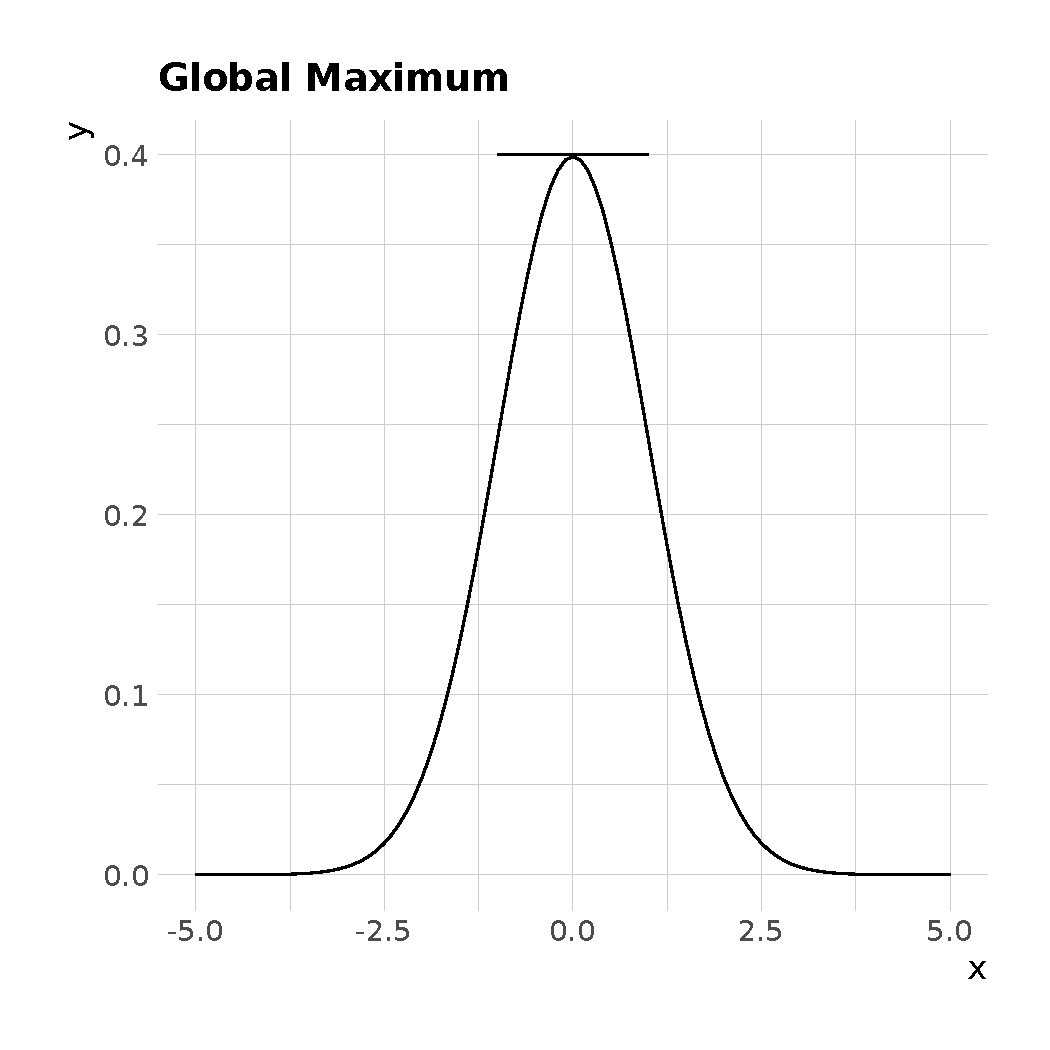
\includegraphics[scale = 0.55]{figures/optim.pdf}
    \caption{Visualizing how a derivative is equal to 0 at a function's maximum or minimum.}
    \label{fig:optim}
\end{figure}

\begin{itemize}
    \item \textbf{First-order condition}: $f'(x) = 0$
    \begin{itemize}
        \item Maximum or minimum
        \item This assumes that $f(x)$ is differentiable at all values -- it is a continuous function.
    \end{itemize}
    \item \textbf{Second-order condition}: $f''(x)$, where $>0$ means minimum, $<0$ means maximum, and $=0$ an inflection point.
\end{itemize}

\begin{align*}
    f(x) & = x^2 - 4x -1 \\
    \text{FOC: } f'(x) & = 2x -4 \\
    x & = 2 \\
    \text{SOC: } f''(x) & = 2 \Rightarrow \text{minimum}
\end{align*}

\noindent What if we have multiple variables?

\begin{itemize}
    \item Let $f(x) = -x_1^2 + x_1x_2 - x_2^2$ 
    \begin{itemize}
        \item FOC: 
        \begin{itemize}
            \item $f_{x_1} = -2x_1 + x_2 = 0$
            \item $f_{x_2} = x_1 - 2x_2 = 0$ 
            
            \vspace{1em}
            $\begin{bmatrix}[cc|c]
                    -2 & 1 & 0 \\
                    1 & -2 & 0
            \end{bmatrix}$
            \vspace{1em}

            \begin{itemize}
                \item It turns out $x_1 = 0$, $x_2 = 0$
            \end{itemize} 
        \end{itemize} 
        \item SOC: We need to build the hessian:
        
        \vspace{1em}
        $\begin{bmatrix}
            \frac{d^2f}{dx_1x_1} & \frac{d^2}{dx_1x_2} \\ \\
            \frac{d^2f}{dx_2x_1} & \frac{d^2f}{dx_2x_2}
        \end{bmatrix}
        = 
        \begin{bmatrix}
            -2 & 1 \\
            1 & -2
        \end{bmatrix}
        $
        \vspace{1em}
    \end{itemize}
    \item Now, we ask whether these points are minima, maxima, indeterminate, or saddle points. 
    \begin{itemize}
        \item We calculate the determinants of each ``principal minor''.
        \item PM$_1 = -2$, $D_1 = -2$
        \item PM$_2 = \begin{bmatrix}
            -2 & 1 \\
            1 & -2
        \end{bmatrix}$, $D_2 = (-2 \cdot -2) - (1 \cdot 1) = 3$
    \end{itemize}
    \item The hessian is:
    \begin{itemize}
        \item Positive definite: $D_1 > 0$, $D_2 > 0$, strictly local minima
        \item Negative definite: $D_1 < 0$, $D_2 > 0$, strictly local maxima
        \begin{itemize}
            \item Start negative and then alternate signs
        \end{itemize} 
        \item Positive semi-definite: $D_1 \geq 0$, $D_2 \geq 0$
        \item Negative semi-definite: $D_1 \leq 0$, $D_2 \geq 0$
    \end{itemize}
    \item For larger matrices?
    \begin{itemize}
        \item $\begin{bmatrix}
            .
        \end{bmatrix}$, PM$_1 = $ determinant of $1 \times 1$
        \item $\begin{bmatrix}
            . & . \\
            . & .
        \end{bmatrix}$, PM$_2 = $ determinant of $2 \times 2$
        \item $\begin{bmatrix}
            . & . & .\\
            . & . & . \\
            . & . & .
        \end{bmatrix}$, PM$_3 = $ determinant of $3 \times 3$
    \end{itemize}
    \item If we have a $3 \times 3$ matrix:
    \begin{itemize}
        \item PD: D$_1 > 0$, D$_2 > 0$, D$_3 > 0$
        \item ND: D$_1 < 0$, D$_2 > 0$, D$_3 < 0$
        \item PSD: D$_1 \geq 0$, D$_2 \geq 0$, D$_3 \geq 0$
        \item NSD: D$_1 \leq 0$, D$_2 \geq 0$, D$_3 \leq 0$
    \end{itemize}
\end{itemize}


\subsection{Constrained Optimization -- Lagrange Multiplier}

Sometimes, we have to find the maxima or minima under set conditions. 

\begin{align*}
    & \text{Max } f(x_1, x_2) \text{ s.t. } g(x_1, x_2) = 0 \\
    & \text{Max } f(x_1, x_2) - \lambda g(x_1, x_2)
\end{align*}

\begin{itemize}
    \item $\lambda$ is us creating a new variable.
    \item FOC: 
    \begin{align*}
        f_{x_1} - \lambda g_{x_1} = & \, 0 \\
        f_{x_2} - \lambda g_{x_1} = & \, 0 \\
        g(x_1, x_2) = & \, 0 \\
    \end{align*}
        \item Then:
    \begin{align*}
        f(x_1, x_2) = & 36 - x_1^2 - x_2^2, \, \, g(x_1, x_2) = x_1 + 7x_2 - 25  \\ 
        f(x_1, x_2, \lambda) = & 36 - x_1^2 - x_2^2 - \lambda(x1 + 7x_2 - 25) \\
        f_{x_1} & = -2x_1 - \lambda = 0, \Rightarrow x_1 = -\lambda/2 \\
        f_{x_2} & = - 2x^2 - 7\lambda = 0, \Rightarrow x_2 = -7\lambda/2 \\
        g(x_1, x_2) & = -\lambda/2 + -7\lambda/2 - 25 = 0 \\ 
        \lambda & = -1 \\
        \text{Therefore: } & x_1 = \frac{1}{2}, x_2 = \frac{7}{2} 
    \end{align*}
\end{itemize}

\subsection{Integration}

\begin{itemize}
    \item $f(x) = 40x$
    \item $F(x) = 20x^2 + c$
    \begin{itemize}
        \item This is the `antiderivative', $F'(x) = f(x)$, because if $F(X)$ is derived then it returns $f(x)$.
        \item We add c because any constant will turn to 0 when the derivative is taken. 
    \end{itemize}
    \item Powerfully, antidifferentiation lets us solve for the value of $y$, given $dy/dx$.
\end{itemize}

\begin{itemize}
    \item \textbf{Rules of integration}
    \begin{itemize}
        \item Power rule: $f(x) = x^n$, $F(x) = \frac{1}{n + 1} x^{n + 1} + c$
        \item Exponent rule: $f(x) = e^x$, $F(x) = e^x + c$
        \begin{itemize}
            \item But: $f(x) = e^ax$, $F(x) = \frac{1}{a}e^{ax} + c$
        \end{itemize}
        \item Logarithm rule: $f(x) = \frac{1}{x}$, $F(x) = ln(x) + c$
        \item Chain rule: $f(x) = g'(x)e^{g(x)}$, $F(x) = e^{g(x)} + c$
        \item Chain + log: $f(x) = \frac{g'(x)}{g(x)}$, $F(x) = ln|g(x)| + c$
        \item Sum rule: $f(x) = g(x) + h(x)$, $F(x) = G(x) + H(x)$
        \item Constant rule: $f(x) = kg(x)$, $F(x) = k G(x)$ 
        \item Integral of a constant: $f(x) = k$, $F(x) = kx + c$
    \end{itemize}
\end{itemize}

\noindent We integrate so that we can add continuously. The integral is the limit of the sum, where we add all slices under the curve until we reach infinity. We end up summing the values of infinitesimally small ranges. This is the idea behind Riemann sums.


\subsection{Areas and Riemann Sums}

Consider the following function

\begin{center}
    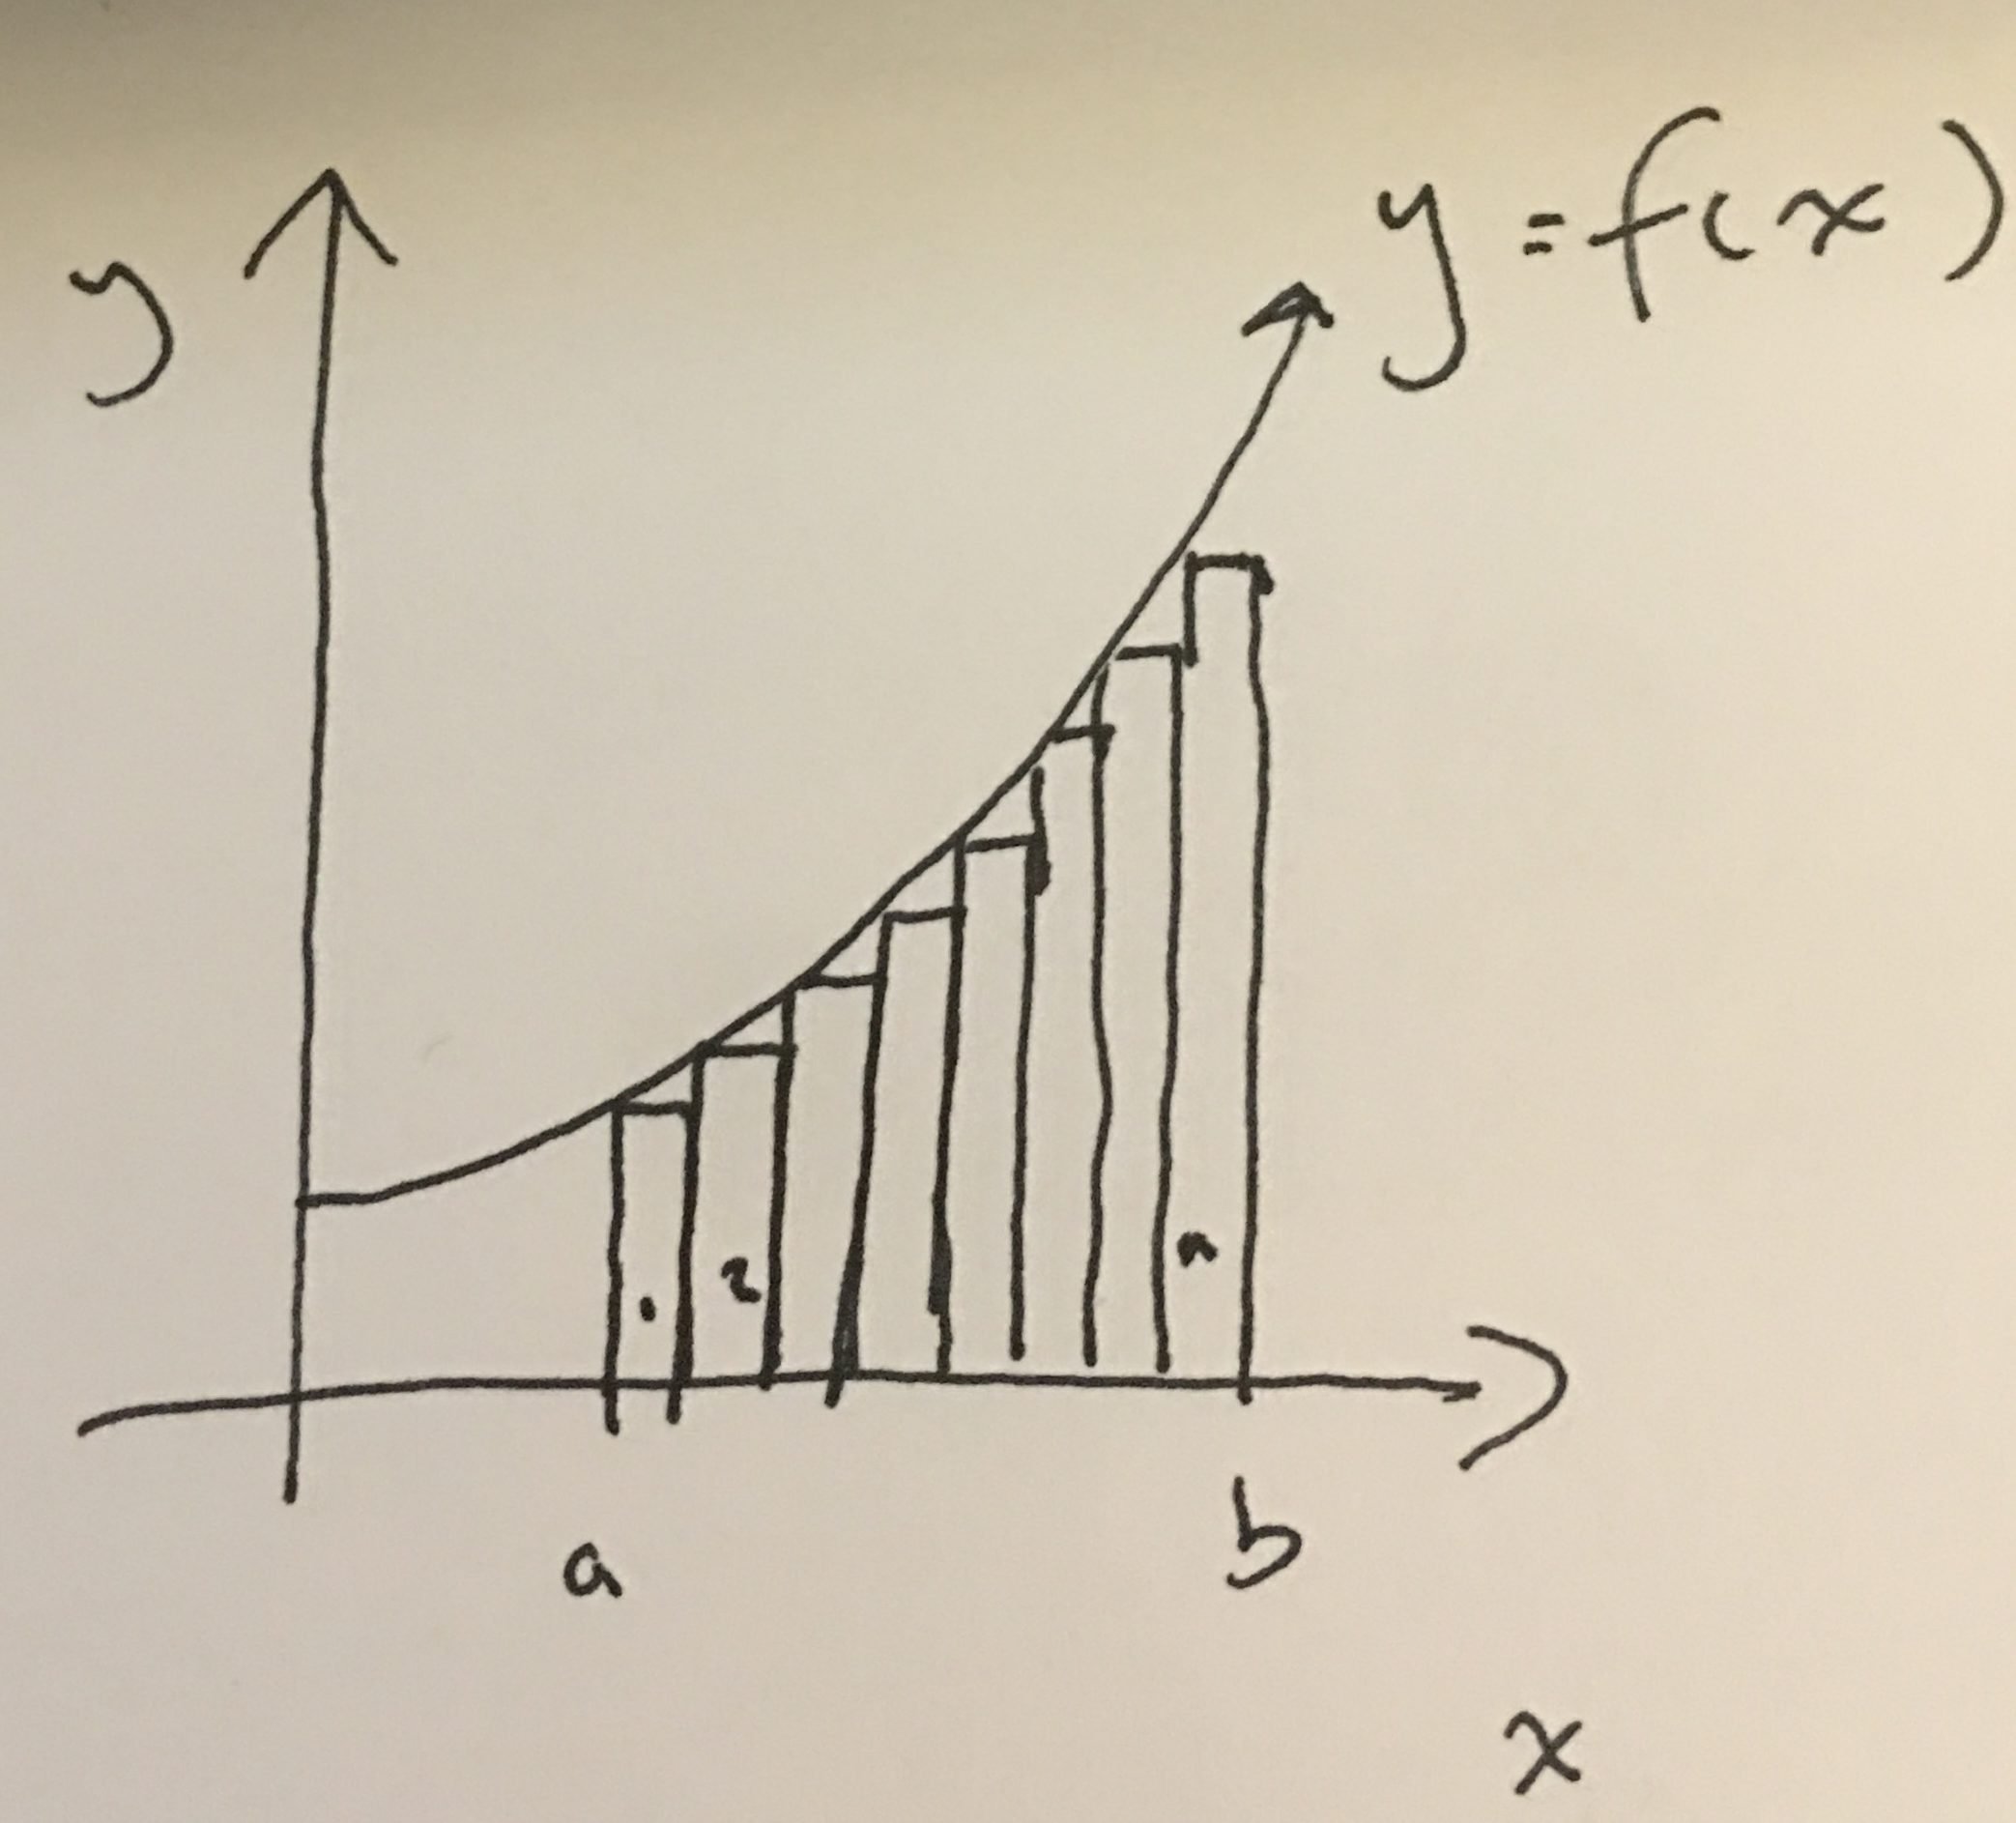
\includegraphics[scale = 0.075]{figures/riemann_ex.png}    
\end{center}

\noindent where $\sum_{u=1}^n f(x_i)\Delta x$ and $\Delta x = \frac{b - a}{n}$. This equals the sum of the area of all the rectangles under $f(x)$. The closer $n$ gets to $\infty$, then the closer the sum of all the areas gets to the area under $f(x)$ from $a$ to $b$. 

\vspace{1em}

\noindent It also turns out that 

\begin{equation*}
    \lim_{n \rightarrow \infty} \sum_{i = 1}^n f(x_i) \Delta x = \int_{b}^a f(x)dx
\end{equation*}

\noindent Because of this, we can use a definite integral to calculate the area under a function/curve between two points.


\newpage

% Lecture 9: Calculus IV
\section{Calculus IV}

\subsection{Fundamental Theorem of Calculus}

This brings us to the grandiose titled fundamental theorem of calculus: 

\vspace{-1em}
\begin{equation*}
    \int_a^b f(x)dx = F(b) - F(a)
\end{equation*}

\noindent Where the difference between the antiderivative at two points gives us the area under a curve between these two values. This is given such importance because it links derivatives and integrals. 

\noindent Ex:

\begin{equation*}
    \int_1^3 x^2dx = \frac{1}{3}x^3 \Big\rvert_1^3 = \frac{27}{3} - \frac{1}{3} = \frac{26}{3}
\end{equation*}

\subsection{Rules for definite integrals}

\begin{enumerate}
    \item \begin{equation*}
        \int_a^b f(x)d(x) = - \int_b^a f(x)dx
    \end{equation*}
    
    \item \begin{equation*}
        \int_a^d f(x)dx = \int_a^b f(x)dx + \int_b^c f(x)dx + \int_c^d f(x)dx \, \, \, \text{ where } \, \, \, a \leq b \leq c \leq d
    \end{equation*}

    \item \begin{equation*}
        \int_a^b - f(x)dx = - \int_a^b f(x)dx
    \end{equation*}

    \item \begin{equation*}
        \int_a^b k f(x)dx = k \int_a^b f(x)dx
    \end{equation*}

    \item \begin{equation*}
        \int_a^b \left[f(x) \pm g(x)\right]dx = \int_a^b f(x)dx \pm \int_a^b g(x)dx
    \end{equation*}
\end{enumerate}

\subsection{Integration by substitution}

\begin{enumerate}
    \item Define a new variable, $u = G(x)$ such that when written in terms of $u$ the integrand is simpler.
    \item Integrate the function, changing the limits of the integral to be from $a$ and $b$ to $g(a)$ or $g(b)$.
    \item Rewrite in terms of $x$.
\end{enumerate}

Ex:

\begin{align*}
    \int_{x=a}^{x=b} 8x(x^2 + 1)^3dx
\end{align*}

\begin{itemize}
    \item Let $u = x^2 + 1$
    \item Then, $\frac{du}{dx} = 2x$
    \item And: $\frac{1}{2x}du = dx$. So we can rewrite the above function as:
\end{itemize}

\vspace{-1em}

\begin{equation*}
    \int_a^b 8xu^3 \cdot \frac{1}{2x}
    du
\end{equation*}

We simplify to change the limits to reflect $g(u)$.

\vspace{-1em}

\begin{align*}
    & \int_{a^2 + 1}^{b^2 + 1} 4u^3 du \\
    & =  \int_{a^2 + 1}^{b^2 + 1} \frac{4}{4}u^4 = u^4 \Big\vert_{a^2 + 1}^{b^2 + 1}
\end{align*}

Then we rewrite in terms of x:

\vspace{-1em}

\begin{equation*}
    (x^2 + 1)^4 \Big\vert_a^b
\end{equation*}  

\subsubsection{Some examples}

\begin{itemize}
    \item 
    \begin{align*}
        & \int_a^b 3x^2 \sqrt{x^3 + 1}dx \\
        & \text{Let } u = x^3 + 1 \\
        & \frac{du}{dx} = 3x^2, \, \, \frac{1}{3x^2}du = dx \\
        & = \int_{a^3+1}^{b^3 + 1} 3x^2 \sqrt{u}\frac{1}{3x^2}du \\
        & = \int_{a^3 + 1}^{b^3 + 1} \sqrt{u}\,du = \int_{a^3 + 1}^{b^3 + 1} u^{\frac{1}{2}}du \\
        & = \frac{2}{3}u^{\frac{3}{2}}\Big\vert_{a^3 + 1}^{b^3 + 1} = \frac{2}{3}(x^3 + 1)^{\frac{3}{2}} \Big\vert_a^b
    \end{align*}

    \item 
    \begin{align*}
        & \int_a^b x^3e^{x^3}dx \\
        & \text{Let } u = x^3, \frac{du}{dx} = 3x^2, dx = \frac{du}{3x^2} \\
        & \int_{a^3}^{b^3} x^2e^u \frac{du}{3x^2} = \frac{1}{3}\int_{a^3}^{b^3} e^u du \\
        & = \frac{1}{3} e^u \Big\vert_{a^3}^{b^3} = \frac{1}{3}e^{x^3}\Big\vert_{a}^{b}
    \end{align*}

    \item 
    \begin{align*}
        & \int_a^b \frac{2 - x}{\sqrt{2x^2 - 8x + 1}}dx \\
        & \text{Let } u = 2x^2 - 8x + 1 \\
        & \frac{du}{dx} = 4x - 8, dx = \frac{du}{4x - 8} \\
        & \int (2 - x)u^{-\frac{1}{2}}\frac{du}{-4(2-x)} = - \frac{1}{4}\int u^{-\frac{1}{2}}du \\
        & = -\frac{1}{4} \cdot \frac{u^{\frac{1}{2}}}{\frac{1}{2}} \\
        & -\frac{1}{2}u^{\frac{1}{2}}\Big\vert_a^b
    \end{align*}
\end{itemize}

\subsection{Integration by parts}

Sometimes we get functions where integrating by substitution does not gain us any leverage. For these, we can \emph{integrate by parts}. Say we have two functions $u$ and $v$, which are differentiable. We can use the product rule to show that:

\begin{equation*}
    \frac{d}{dx}(uv) = v \frac{du}{dx} + u \frac{dv}{dx} 
\end{equation*}

And rearrange: 

\begin{equation*}
    u \frac{dv}{dx} = \frac{d}{dx}(uv) - v \frac{du}{dx}
\end{equation*}

Integrate with respect to $x$, and we get the formula for integration by parts:

\begin{equation*}
    \int u dv = uv - \int v du
\end{equation*}

An example: 

\begin{align*}
    &\int_a^b x^2 \text{ln}x dx \\
    &u = \text{ln}x \Rightarrow du = \frac{1}{x}dx \\
    &dv = x^2 dx \text{ Integrate } \Rightarrow v = \frac{x^3}{3} \\
    &\text{So the original equation equals:} \\
    &\frac{1}{3}x^3 \text{ln}x - \int\frac{1}{3}x^3 \cdot\frac{1}{x}dx \\
    & = \frac{1}{3}x^3 \text{ln}x - \frac{1}{3}\int x^2 dx = \left[\frac{1}{3}x^3 \text{ln}x - \frac{1}{3}\cdot\frac{1}{3}x^3\right]_a^b
\end{align*}

One more: 

\begin{align*}
    & \int_1^3 xe^x dx \\
    & u = x, du = dx, dv = e^xdx, v = e^x \\
    & \int_1^3 xe^x dx = xe^x - \int e^xdx \\ 
    & = \left[xe^x - e^x\right]_1^3
\end{align*}


\subsection{Improper integrals}

What if we integrate to $\infty$ instead of a integer? We take the limit when we get to plugging our bounds in.

\begin{align*}
    & \int_1^\infty \frac{1}{\lambda}e^{-\lambda x}dx \\
    & = \frac{1}{\lambda}\int_1^\infty -\frac{1}{\lambda} e^{\lambda x} = \left[-\frac{1}{\lambda^2}e^{-\lambda x}\right]_1^3 \\ 
    & = \left[\lim_{x \rightarrow \infty} -\frac{1}{\lambda^2} e^{-\lambda x}\right] - \left[-\frac{1}{\lambda^2} e^{-\lambda 1}\right] \\
    & = 0 + \left[\frac{1}{\lambda^2} e^{-\lambda}\right]
\end{align*}

\newpage

% Lecture 10: Calculus V
\section{Calculus V}

\subsection{Double Integrals}

Sometimes we want to integrate the area of a function depending on multiple variables. In this case we can take a double integral. We just take the integral of the function with respect to one variable. And then we integrate the outcome with respect to another variable:

\begin{align*}
    & \int_{x_2 = 0}^1 \int_{x_1 = -1}^1 (x_1^2 + x_2^2) d x_1 d x_2 \\
    = & \int_0^1 \left[\int_{-1}^1 (x_1^2 + x_2^2) d x_1 \right]d x_2 \\
    = & \int_0^1 \left[ \frac{1}{3}x_1^3 + x_1x_2^2 \right]_{-1}^1 d x_2 \\
    = & \int_0^1 \left\{\left[ \frac{1}{3}1^3 + 1x_2^2 \right]
        - \left[\frac{1}{3}-1^3 + (-1)x_2^2\right]\right\}d x_2 \\
    = & \int_0^1 \left(\frac{2}{3} + 2x_2^2\right) d x_2 \\
    = & \left[\frac{2}{3}x_2 + \frac{2}{3}x_2^3\right]_0^1 \\
    = & \frac{4}{3}
\end{align*}
% Now wrap-up test


\newpage
\bibliographystyle{abbrvnat}
\bibliography{math_lectures}


\end{document}
